\PassOptionsToPackage{unicode=true}{hyperref} % options for packages loaded elsewhere
\PassOptionsToPackage{hyphens}{url}
%
\documentclass[]{book}
\usepackage{lmodern}
\usepackage{amssymb,amsmath}
\usepackage{ifxetex,ifluatex}
\usepackage{fixltx2e} % provides \textsubscript
\ifnum 0\ifxetex 1\fi\ifluatex 1\fi=0 % if pdftex
  \usepackage[T1]{fontenc}
  \usepackage[utf8]{inputenc}
  \usepackage{textcomp} % provides euro and other symbols
\else % if luatex or xelatex
  \usepackage{unicode-math}
  \defaultfontfeatures{Ligatures=TeX,Scale=MatchLowercase}
\fi
% use upquote if available, for straight quotes in verbatim environments
\IfFileExists{upquote.sty}{\usepackage{upquote}}{}
% use microtype if available
\IfFileExists{microtype.sty}{%
\usepackage[]{microtype}
\UseMicrotypeSet[protrusion]{basicmath} % disable protrusion for tt fonts
}{}
\IfFileExists{parskip.sty}{%
\usepackage{parskip}
}{% else
\setlength{\parindent}{0pt}
\setlength{\parskip}{6pt plus 2pt minus 1pt}
}
\usepackage{hyperref}
\hypersetup{
            pdftitle={Diagnostics Supplemental Material},
            pdfauthor={Jose Guadalupe Hernandez},
            pdfborder={0 0 0},
            breaklinks=true}
\urlstyle{same}  % don't use monospace font for urls
\usepackage{color}
\usepackage{fancyvrb}
\newcommand{\VerbBar}{|}
\newcommand{\VERB}{\Verb[commandchars=\\\{\}]}
\DefineVerbatimEnvironment{Highlighting}{Verbatim}{commandchars=\\\{\}}
% Add ',fontsize=\small' for more characters per line
\usepackage{framed}
\definecolor{shadecolor}{RGB}{248,248,248}
\newenvironment{Shaded}{\begin{snugshade}}{\end{snugshade}}
\newcommand{\AlertTok}[1]{\textcolor[rgb]{0.94,0.16,0.16}{#1}}
\newcommand{\AnnotationTok}[1]{\textcolor[rgb]{0.56,0.35,0.01}{\textbf{\textit{#1}}}}
\newcommand{\AttributeTok}[1]{\textcolor[rgb]{0.77,0.63,0.00}{#1}}
\newcommand{\BaseNTok}[1]{\textcolor[rgb]{0.00,0.00,0.81}{#1}}
\newcommand{\BuiltInTok}[1]{#1}
\newcommand{\CharTok}[1]{\textcolor[rgb]{0.31,0.60,0.02}{#1}}
\newcommand{\CommentTok}[1]{\textcolor[rgb]{0.56,0.35,0.01}{\textit{#1}}}
\newcommand{\CommentVarTok}[1]{\textcolor[rgb]{0.56,0.35,0.01}{\textbf{\textit{#1}}}}
\newcommand{\ConstantTok}[1]{\textcolor[rgb]{0.00,0.00,0.00}{#1}}
\newcommand{\ControlFlowTok}[1]{\textcolor[rgb]{0.13,0.29,0.53}{\textbf{#1}}}
\newcommand{\DataTypeTok}[1]{\textcolor[rgb]{0.13,0.29,0.53}{#1}}
\newcommand{\DecValTok}[1]{\textcolor[rgb]{0.00,0.00,0.81}{#1}}
\newcommand{\DocumentationTok}[1]{\textcolor[rgb]{0.56,0.35,0.01}{\textbf{\textit{#1}}}}
\newcommand{\ErrorTok}[1]{\textcolor[rgb]{0.64,0.00,0.00}{\textbf{#1}}}
\newcommand{\ExtensionTok}[1]{#1}
\newcommand{\FloatTok}[1]{\textcolor[rgb]{0.00,0.00,0.81}{#1}}
\newcommand{\FunctionTok}[1]{\textcolor[rgb]{0.00,0.00,0.00}{#1}}
\newcommand{\ImportTok}[1]{#1}
\newcommand{\InformationTok}[1]{\textcolor[rgb]{0.56,0.35,0.01}{\textbf{\textit{#1}}}}
\newcommand{\KeywordTok}[1]{\textcolor[rgb]{0.13,0.29,0.53}{\textbf{#1}}}
\newcommand{\NormalTok}[1]{#1}
\newcommand{\OperatorTok}[1]{\textcolor[rgb]{0.81,0.36,0.00}{\textbf{#1}}}
\newcommand{\OtherTok}[1]{\textcolor[rgb]{0.56,0.35,0.01}{#1}}
\newcommand{\PreprocessorTok}[1]{\textcolor[rgb]{0.56,0.35,0.01}{\textit{#1}}}
\newcommand{\RegionMarkerTok}[1]{#1}
\newcommand{\SpecialCharTok}[1]{\textcolor[rgb]{0.00,0.00,0.00}{#1}}
\newcommand{\SpecialStringTok}[1]{\textcolor[rgb]{0.31,0.60,0.02}{#1}}
\newcommand{\StringTok}[1]{\textcolor[rgb]{0.31,0.60,0.02}{#1}}
\newcommand{\VariableTok}[1]{\textcolor[rgb]{0.00,0.00,0.00}{#1}}
\newcommand{\VerbatimStringTok}[1]{\textcolor[rgb]{0.31,0.60,0.02}{#1}}
\newcommand{\WarningTok}[1]{\textcolor[rgb]{0.56,0.35,0.01}{\textbf{\textit{#1}}}}
\usepackage{longtable,booktabs}
% Fix footnotes in tables (requires footnote package)
\IfFileExists{footnote.sty}{\usepackage{footnote}\makesavenoteenv{longtable}}{}
\usepackage{graphicx,grffile}
\makeatletter
\def\maxwidth{\ifdim\Gin@nat@width>\linewidth\linewidth\else\Gin@nat@width\fi}
\def\maxheight{\ifdim\Gin@nat@height>\textheight\textheight\else\Gin@nat@height\fi}
\makeatother
% Scale images if necessary, so that they will not overflow the page
% margins by default, and it is still possible to overwrite the defaults
% using explicit options in \includegraphics[width, height, ...]{}
\setkeys{Gin}{width=\maxwidth,height=\maxheight,keepaspectratio}
\setlength{\emergencystretch}{3em}  % prevent overfull lines
\providecommand{\tightlist}{%
  \setlength{\itemsep}{0pt}\setlength{\parskip}{0pt}}
\setcounter{secnumdepth}{5}
% Redefines (sub)paragraphs to behave more like sections
\ifx\paragraph\undefined\else
\let\oldparagraph\paragraph
\renewcommand{\paragraph}[1]{\oldparagraph{#1}\mbox{}}
\fi
\ifx\subparagraph\undefined\else
\let\oldsubparagraph\subparagraph
\renewcommand{\subparagraph}[1]{\oldsubparagraph{#1}\mbox{}}
\fi

% set default figure placement to htbp
\makeatletter
\def\fps@figure{htbp}
\makeatother

\usepackage[]{natbib}
\bibliographystyle{apalike}

\title{Diagnostics Supplemental Material}
\author{Jose Guadalupe Hernandez}
\date{2022-08-04}

\begin{document}
\maketitle

{
\setcounter{tocdepth}{1}
\tableofcontents
}
\hypertarget{introduction}{%
\chapter{Introduction}\label{introduction}}

This is the supplemental material associated with our 2022 ECJ contribution entitled, \emph{A suite of diagnostic metrics for characterizing selection schemes}.
Preprint \href{https://arxiv.org/pdf/2204.13839.pdf}{here}.

\hypertarget{about-our-supplemental-material}{%
\section{About our supplemental material}\label{about-our-supplemental-material}}

This supplemental material is hosted on \href{https://github.com}{GitHub} using GitHub pages.
The source code and configuration files used to generate this supplemental material can be found in \href{https://github.com/jgh9094/ECJ-2022-suite-of-diagnostics-for-selection-schemes}{this GitHub repository}.
We compiled our data analyses and supplemental documentation into this nifty web-accessible book using \href{https://bookdown.org/}{bookdown}.

Our supplemental material includes the following paper figures and statistics:

\begin{itemize}
\tightlist
\item
  Exploitation rate results (Section \ref{exploitation-rate-results})
\item
  Ordered exploitation results (Section \ref{ordered-exploitation-results})
\item
  Contradictory objectives results (Section \ref{contradictory-objectives-results})
\item
  Multi-path exploration results (Section \ref{multi-path-exploration-results})
\end{itemize}

Additionally, our supplemental material includes the results from parameter tuning selection schemes:

\begin{itemize}
\tightlist
\item
  Truncation selection (Section \ref{truncation-selection})
\item
  Tournament selection sharing (Section \ref{tournament-selection})
\item
  Genotypic fitness sharing (Section \ref{genotypic-fitness-sharing})
\item
  Phenotypic fitness sharing (Section \ref{phenotypic-fitness-sharing})
\item
  Nondominated sorting (Section \ref{nondominated-sorting})
\item
  Novelty search (Section \ref{novelty-search})
\end{itemize}

\hypertarget{contributing-authors}{%
\section{Contributing authors}\label{contributing-authors}}

\begin{itemize}
\tightlist
\item
  \href{https://jgh9094.github.io/}{Jose Guadalupe Hernandez}
\item
  \href{https://lalejini.com}{Alexander Lalejini}
\item
  \href{http://ofria.com}{Charles Ofria}
\end{itemize}

\hypertarget{research-overview}{%
\section{Research overview}\label{research-overview}}

\textbf{Abstract}:

Evolutionary algorithms typically consist of multiple interacting components, where each component influences an algorithm's problem-solving abilities.
Understanding how each component of an evolutionary algorithm influences problem-solving success can improve our ability to target particular problem domains.
Benchmark suites provide insights into an evolutionary algorithm's problem-solving capabilities, but benchmarking problems often have complex search space topologies, making it difficult to isolate and test an algorithm's strengths and weaknesses.
Our work focuses on diagnosing selection schemes, which identify individuals to contribute genetic material to the next generation, thus driving an evolutionary algorithm's search strategy.
We introduce four diagnostics for empirically testing the strengths and weaknesses of selection schemes: the exploitation rate diagnostic, ordered exploitation rate diagnostic, contradictory objectives diagnostic, and the multi-path exploration diagnostic.
Each diagnostic is a handcrafted search space designed to isolate and measure the relative exploitation and exploration characteristics of selection schemes.
Here, we use our diagnostics to evaluate six population selection methods: truncation selection, tournament selection, fitness sharing, lexicase selection, nondominated sorting, and novelty search.
Expectedly, tournament and truncation selection excelled at gradient exploitation but poorly explored search spaces, while novelty search excelled at exploration but failed to exploit gradients.
Fitness sharing performed poorly across all diagnostics, suggesting poor overall exploitation and exploration abilities.
Nondominated sorting was best for maintaining diverse populations comprised of individuals inhabiting multiple optima, but struggled to effectively exploit gradients.
Lexicase selection balanced search space exploration without sacrificing exploitation, generally performing well across diagnostics.
Our work demonstrates the value of diagnostics for building a deeper understanding of selection schemes, which can then be used to improve or develop new selection methods.

\hypertarget{experimental-setup}{%
\section{Experimental setup}\label{experimental-setup}}

Setting up required variables variables.

\begin{Shaded}
\begin{Highlighting}[]
\KeywordTok{library}\NormalTok{(ggplot2)}
\KeywordTok{library}\NormalTok{(dplyr)}
\end{Highlighting}
\end{Shaded}

\begin{verbatim}
## 
## Attaching package: 'dplyr'
\end{verbatim}

\begin{verbatim}
## The following objects are masked from 'package:stats':
## 
##     filter, lag
\end{verbatim}

\begin{verbatim}
## The following objects are masked from 'package:base':
## 
##     intersect, setdiff, setequal, union
\end{verbatim}

\begin{Shaded}
\begin{Highlighting}[]
\CommentTok{# variables used throughout}
\NormalTok{TRAITS =}\StringTok{ }\DecValTok{100}
\NormalTok{TSIZE =}\StringTok{ }\DecValTok{26}
\NormalTok{ORDER =}\StringTok{ }\KeywordTok{c}\NormalTok{(}\StringTok{'Truncation (tru)'}\NormalTok{,}\StringTok{'Tournament (tor)'}\NormalTok{, }\StringTok{'Genotypic Fitness Sharing (gfs)'}\NormalTok{,}\StringTok{'Phenotypic Fitness Sharing (pfs)'}\NormalTok{,}\StringTok{'Lexicase (lex)'}\NormalTok{,}\StringTok{'Nondominated Sorting (nds)'}\NormalTok{,}\StringTok{'Novelty Search (nov)'}\NormalTok{,}\StringTok{'Random (ran)'}\NormalTok{)}
\NormalTok{ACRON =}\StringTok{ }\KeywordTok{tolower}\NormalTok{(}\KeywordTok{c}\NormalTok{(}\StringTok{'TRU'}\NormalTok{,}\StringTok{'TOR'}\NormalTok{,}\StringTok{'GFS'}\NormalTok{,}\StringTok{'PFS'}\NormalTok{,}\StringTok{'LEX'}\NormalTok{,}\StringTok{'NDS'}\NormalTok{,}\StringTok{'NOV'}\NormalTok{,}\StringTok{'RAN'}\NormalTok{))}
\NormalTok{SHAPE =}\StringTok{ }\KeywordTok{c}\NormalTok{(}\DecValTok{5}\NormalTok{,}\DecValTok{3}\NormalTok{,}\DecValTok{2}\NormalTok{,}\DecValTok{6}\NormalTok{,}\DecValTok{1}\NormalTok{,}\DecValTok{0}\NormalTok{,}\DecValTok{4}\NormalTok{,}\DecValTok{20}\NormalTok{,}\DecValTok{1}\NormalTok{)}
\NormalTok{PARAM =}\StringTok{ }\KeywordTok{c}\NormalTok{(}\StringTok{'8'}\NormalTok{, }\StringTok{'8'}\NormalTok{, }\StringTok{'0.3'}\NormalTok{, }\StringTok{'0.3'}\NormalTok{, }\StringTok{'0.0'}\NormalTok{, }\StringTok{'0.3'}\NormalTok{, }\StringTok{'15'}\NormalTok{, }\StringTok{'1'}\NormalTok{)}
\NormalTok{cb_palette <-}\StringTok{ }\KeywordTok{c}\NormalTok{(}\StringTok{'#332288'}\NormalTok{,}\StringTok{'#88CCEE'}\NormalTok{,}\StringTok{'#EE3377'}\NormalTok{,}\StringTok{'#117733'}\NormalTok{,}\StringTok{'#EE7733'}\NormalTok{,}\StringTok{'#882255'}\NormalTok{,}\StringTok{'#44AA99'}\NormalTok{,}\StringTok{'#CCBB44'}\NormalTok{, }\StringTok{'#000000'}\NormalTok{)}

\CommentTok{# selection scheme parameters}
\NormalTok{TR_LIST =}\StringTok{ }\KeywordTok{c}\NormalTok{(}\DecValTok{1}\NormalTok{, }\DecValTok{2}\NormalTok{, }\DecValTok{4}\NormalTok{, }\DecValTok{8}\NormalTok{, }\DecValTok{16}\NormalTok{, }\DecValTok{32}\NormalTok{, }\DecValTok{64}\NormalTok{, }\DecValTok{128}\NormalTok{, }\DecValTok{256}\NormalTok{)}
\NormalTok{TS_LIST =}\StringTok{ }\KeywordTok{c}\NormalTok{(}\DecValTok{2}\NormalTok{, }\DecValTok{4}\NormalTok{, }\DecValTok{8}\NormalTok{, }\DecValTok{16}\NormalTok{, }\DecValTok{32}\NormalTok{, }\DecValTok{64}\NormalTok{, }\DecValTok{128}\NormalTok{, }\DecValTok{256}\NormalTok{)}
\NormalTok{FS_LIST =}\StringTok{ }\KeywordTok{c}\NormalTok{(}\FloatTok{0.0}\NormalTok{, }\FloatTok{0.1}\NormalTok{, }\FloatTok{0.3}\NormalTok{, }\FloatTok{0.6}\NormalTok{, }\FloatTok{1.2}\NormalTok{, }\FloatTok{2.5}\NormalTok{, }\FloatTok{5.0}\NormalTok{)}
\NormalTok{ND_LIST =}\StringTok{ }\KeywordTok{c}\NormalTok{(}\FloatTok{0.0}\NormalTok{, }\FloatTok{0.1}\NormalTok{, }\FloatTok{0.3}\NormalTok{, }\FloatTok{0.6}\NormalTok{, }\FloatTok{1.2}\NormalTok{, }\FloatTok{2.5}\NormalTok{, }\FloatTok{5.0}\NormalTok{)}
\NormalTok{NS_LIST =}\StringTok{ }\KeywordTok{c}\NormalTok{(}\DecValTok{1}\NormalTok{, }\DecValTok{2}\NormalTok{, }\DecValTok{4}\NormalTok{, }\DecValTok{8}\NormalTok{, }\DecValTok{15}\NormalTok{, }\DecValTok{30}\NormalTok{)}

\CommentTok{# theme that graphs will follow}
\NormalTok{p_theme <-}\StringTok{ }\KeywordTok{theme}\NormalTok{(}
  \DataTypeTok{text =} \KeywordTok{element_text}\NormalTok{(}\DataTypeTok{size =} \DecValTok{28}\NormalTok{),}
  \DataTypeTok{plot.title =} \KeywordTok{element_text}\NormalTok{( }\DataTypeTok{face =} \StringTok{"bold"}\NormalTok{, }\DataTypeTok{size =} \DecValTok{22}\NormalTok{, }\DataTypeTok{hjust=}\FloatTok{0.5}\NormalTok{),}
  \DataTypeTok{panel.border =} \KeywordTok{element_blank}\NormalTok{(),}
  \DataTypeTok{panel.grid.minor =} \KeywordTok{element_blank}\NormalTok{(),}
  \DataTypeTok{legend.title=}\KeywordTok{element_text}\NormalTok{(}\DataTypeTok{size=}\DecValTok{18}\NormalTok{),}
  \DataTypeTok{legend.text=}\KeywordTok{element_text}\NormalTok{(}\DataTypeTok{size=}\DecValTok{14}\NormalTok{),}
  \DataTypeTok{axis.title =} \KeywordTok{element_text}\NormalTok{(}\DataTypeTok{size=}\DecValTok{18}\NormalTok{),}
  \DataTypeTok{axis.text =} \KeywordTok{element_text}\NormalTok{(}\DataTypeTok{size=}\DecValTok{16}\NormalTok{),}
  \DataTypeTok{legend.position=}\StringTok{"bottom"}\NormalTok{,}
  \DataTypeTok{panel.background =} \KeywordTok{element_rect}\NormalTok{(}\DataTypeTok{fill =} \StringTok{"#f1f2f5"}\NormalTok{,}
                                  \DataTypeTok{colour =} \StringTok{"white"}\NormalTok{,}
                                  \DataTypeTok{size =} \FloatTok{0.5}\NormalTok{, }\DataTypeTok{linetype =} \StringTok{"solid"}\NormalTok{)}
\NormalTok{)}

\CommentTok{# cross comparison data frames}
\NormalTok{cc_over_time <-}\StringTok{ }\KeywordTok{read.csv}\NormalTok{(}\StringTok{'/opt/ECJ-2022-suite-of-diagnostics-for-selection-schemes/DATA-FINAL/POLISHED/cross-comp-over-time.csv'}\NormalTok{, }\DataTypeTok{header =} \OtherTok{TRUE}\NormalTok{, }\DataTypeTok{stringsAsFactors =} \OtherTok{FALSE}\NormalTok{)}
\KeywordTok{colnames}\NormalTok{(cc_over_time)[}\DecValTok{19}\NormalTok{] <-}\StringTok{ 'Selection}\CharTok{\textbackslash{}n}\StringTok{Scheme'}
\NormalTok{cc_over_time}\OperatorTok{$}\StringTok{`}\DataTypeTok{Selection}\CharTok{\textbackslash{}n}\DataTypeTok{Scheme}\StringTok{`}\NormalTok{ <-}\StringTok{ }\KeywordTok{factor}\NormalTok{(cc_over_time}\OperatorTok{$}\StringTok{`}\DataTypeTok{Selection}\CharTok{\textbackslash{}n}\DataTypeTok{Scheme}\StringTok{`}\NormalTok{, }\DataTypeTok{levels =}\NormalTok{ ORDER)}
\NormalTok{cc_best =}\StringTok{ }\KeywordTok{read.csv}\NormalTok{(}\StringTok{'/opt/ECJ-2022-suite-of-diagnostics-for-selection-schemes/DATA-FINAL/POLISHED/cross-comp-best.csv'}\NormalTok{, }\DataTypeTok{header =} \OtherTok{TRUE}\NormalTok{, }\DataTypeTok{stringsAsFactors =} \OtherTok{FALSE}\NormalTok{)}
\NormalTok{cc_best}\OperatorTok{$}\NormalTok{acron <-}\StringTok{ }\KeywordTok{factor}\NormalTok{(cc_best}\OperatorTok{$}\NormalTok{acron, }\DataTypeTok{levels =}\NormalTok{ ACRON)}
\NormalTok{cc_ssf =}\StringTok{ }\KeywordTok{read.csv}\NormalTok{(}\StringTok{'/opt/ECJ-2022-suite-of-diagnostics-for-selection-schemes/DATA-FINAL/POLISHED/selection-scheme-ssf.csv'}\NormalTok{, }\DataTypeTok{header =} \OtherTok{TRUE}\NormalTok{, }\DataTypeTok{stringsAsFactors =} \OtherTok{FALSE}\NormalTok{)}
\NormalTok{cc_ssf}\OperatorTok{$}\NormalTok{acron <-}\StringTok{ }\KeywordTok{factor}\NormalTok{(cc_ssf}\OperatorTok{$}\NormalTok{acron, }\DataTypeTok{levels =}\NormalTok{ ACRON)}
\NormalTok{cc_ssf[}\KeywordTok{is.na}\NormalTok{(cc_ssf)] <-}\StringTok{ }\DecValTok{59999}
\NormalTok{cc_end <-}\StringTok{ }\KeywordTok{filter}\NormalTok{(cc_over_time, gen }\OperatorTok{==}\StringTok{ }\DecValTok{50000}\NormalTok{)}
\NormalTok{cc_end}\OperatorTok{$}\NormalTok{acron <-}\StringTok{ }\KeywordTok{factor}\NormalTok{(cc_end}\OperatorTok{$}\NormalTok{acron, }\DataTypeTok{levels =}\NormalTok{ ACRON)}

\CommentTok{# selection scheme data frames}
\NormalTok{ss_over_time <-}\StringTok{ }\KeywordTok{read.csv}\NormalTok{(}\StringTok{'/opt/ECJ-2022-suite-of-diagnostics-for-selection-schemes/DATA-FINAL/POLISHED/selection-scheme-over-time.csv'}\NormalTok{, }\DataTypeTok{header =} \OtherTok{TRUE}\NormalTok{, }\DataTypeTok{stringsAsFactors =} \OtherTok{FALSE}\NormalTok{)}
\NormalTok{ss_best <-}\StringTok{ }\KeywordTok{read.csv}\NormalTok{(}\StringTok{'/opt/ECJ-2022-suite-of-diagnostics-for-selection-schemes/DATA-FINAL/POLISHED/selection-scheme-best.csv'}\NormalTok{, }\DataTypeTok{header =} \OtherTok{TRUE}\NormalTok{, }\DataTypeTok{stringsAsFactors =} \OtherTok{FALSE}\NormalTok{)}
\NormalTok{ss_ssf <-}\StringTok{ }\KeywordTok{read.csv}\NormalTok{(}\StringTok{'/opt/ECJ-2022-suite-of-diagnostics-for-selection-schemes/DATA-FINAL/POLISHED/selection-scheme-ssf.csv'}\NormalTok{, }\DataTypeTok{header =} \OtherTok{TRUE}\NormalTok{, }\DataTypeTok{stringsAsFactors =} \OtherTok{FALSE}\NormalTok{)}

\CommentTok{## genotypic fitness sharing data frames}
\NormalTok{gfs_ot <-}\StringTok{ }\KeywordTok{filter}\NormalTok{(ss_over_time, acron }\OperatorTok{==}\StringTok{ 'gfs'}\NormalTok{)}
\NormalTok{gfs_ot}\OperatorTok{$}\NormalTok{Sigma <-}\StringTok{ }\KeywordTok{factor}\NormalTok{(gfs_ot}\OperatorTok{$}\NormalTok{trt, }\DataTypeTok{levels =}\NormalTok{ FS_LIST)}
\NormalTok{gfs_best <-}\StringTok{ }\KeywordTok{filter}\NormalTok{(ss_best, acron }\OperatorTok{==}\StringTok{ 'gfs'}\NormalTok{)}
\NormalTok{gfs_best}\OperatorTok{$}\NormalTok{Sigma <-}\StringTok{ }\KeywordTok{factor}\NormalTok{(gfs_best}\OperatorTok{$}\NormalTok{trt, }\DataTypeTok{levels =}\NormalTok{ FS_LIST)}
\NormalTok{gfs_end  <-}\StringTok{ }\KeywordTok{filter}\NormalTok{(gfs_ot, gen }\OperatorTok{==}\StringTok{ }\DecValTok{50000}\NormalTok{)}

\CommentTok{## phenotypic fitness sharing data frames}
\NormalTok{pfs_ot <-}\StringTok{ }\KeywordTok{filter}\NormalTok{(ss_over_time, acron }\OperatorTok{==}\StringTok{ 'pfs'}\NormalTok{)}
\NormalTok{pfs_ot}\OperatorTok{$}\NormalTok{Sigma <-}\StringTok{ }\KeywordTok{factor}\NormalTok{(pfs_ot}\OperatorTok{$}\NormalTok{trt, }\DataTypeTok{levels =}\NormalTok{ FS_LIST)}
\NormalTok{pfs_best <-}\StringTok{ }\KeywordTok{filter}\NormalTok{(ss_best, acron }\OperatorTok{==}\StringTok{ 'pfs'}\NormalTok{)}
\NormalTok{pfs_best}\OperatorTok{$}\NormalTok{Sigma <-}\StringTok{ }\KeywordTok{factor}\NormalTok{(pfs_best}\OperatorTok{$}\NormalTok{trt, }\DataTypeTok{levels =}\NormalTok{ FS_LIST)}
\NormalTok{pfs_end  <-}\StringTok{ }\KeywordTok{filter}\NormalTok{(pfs_ot, gen }\OperatorTok{==}\StringTok{ }\DecValTok{50000}\NormalTok{)}

\CommentTok{## nodominated sorting data frames}
\NormalTok{nds_ot <-}\StringTok{ }\KeywordTok{filter}\NormalTok{(ss_over_time, acron }\OperatorTok{==}\StringTok{ 'nds'}\NormalTok{)}
\NormalTok{nds_ot}\OperatorTok{$}\NormalTok{Sigma <-}\StringTok{ }\KeywordTok{factor}\NormalTok{(nds_ot}\OperatorTok{$}\NormalTok{trt, }\DataTypeTok{levels =}\NormalTok{ ND_LIST)}
\NormalTok{nds_best <-}\StringTok{ }\KeywordTok{filter}\NormalTok{(ss_best, acron }\OperatorTok{==}\StringTok{ 'nds'}\NormalTok{)}
\NormalTok{nds_best}\OperatorTok{$}\NormalTok{Sigma <-}\StringTok{ }\KeywordTok{factor}\NormalTok{(nds_best}\OperatorTok{$}\NormalTok{trt, }\DataTypeTok{levels =}\NormalTok{ ND_LIST)}
\NormalTok{nds_end  <-}\StringTok{ }\KeywordTok{filter}\NormalTok{(nds_ot, gen }\OperatorTok{==}\StringTok{ }\DecValTok{50000}\NormalTok{)}

\CommentTok{## novelty search data frames}
\NormalTok{nov_ot <-}\StringTok{ }\KeywordTok{filter}\NormalTok{(ss_over_time, acron }\OperatorTok{==}\StringTok{ 'nov'} \OperatorTok{&}\StringTok{ }\NormalTok{trt }\OperatorTok{!=}\StringTok{ }\DecValTok{0}\NormalTok{)}
\NormalTok{nov_ot}\OperatorTok{$}\NormalTok{K <-}\StringTok{ }\KeywordTok{factor}\NormalTok{(nov_ot}\OperatorTok{$}\NormalTok{trt, }\DataTypeTok{levels =}\NormalTok{ NS_LIST)}
\NormalTok{nov_best <-}\StringTok{ }\KeywordTok{filter}\NormalTok{(ss_best, acron }\OperatorTok{==}\StringTok{ 'nov'} \OperatorTok{&}\StringTok{ }\NormalTok{trt }\OperatorTok{!=}\StringTok{ }\DecValTok{0}\NormalTok{)}
\NormalTok{nov_best}\OperatorTok{$}\NormalTok{K <-}\StringTok{ }\KeywordTok{factor}\NormalTok{(nov_best}\OperatorTok{$}\NormalTok{trt, }\DataTypeTok{levels =}\NormalTok{ NS_LIST)}
\NormalTok{nov_end  <-}\StringTok{ }\KeywordTok{filter}\NormalTok{(nov_ot, gen }\OperatorTok{==}\StringTok{ }\DecValTok{50000}\NormalTok{)}

\CommentTok{## tournament data frames}
\NormalTok{tor_ot <-}\StringTok{ }\KeywordTok{filter}\NormalTok{(ss_over_time, acron }\OperatorTok{==}\StringTok{ 'tor'} \OperatorTok{&}\StringTok{ }\NormalTok{trt }\OperatorTok{!=}\StringTok{ }\DecValTok{1}\NormalTok{)}
\NormalTok{tor_ot}\OperatorTok{$}\NormalTok{T <-}\StringTok{ }\KeywordTok{factor}\NormalTok{(tor_ot}\OperatorTok{$}\NormalTok{trt, }\DataTypeTok{levels =}\NormalTok{ TS_LIST)}
\NormalTok{tor_best <-}\StringTok{ }\KeywordTok{filter}\NormalTok{(ss_best, acron }\OperatorTok{==}\StringTok{ 'tor'} \OperatorTok{&}\StringTok{ }\NormalTok{trt }\OperatorTok{!=}\StringTok{ }\DecValTok{1}\NormalTok{)}
\NormalTok{tor_best}\OperatorTok{$}\NormalTok{T <-}\StringTok{ }\KeywordTok{factor}\NormalTok{(tor_best}\OperatorTok{$}\NormalTok{trt, }\DataTypeTok{levels =}\NormalTok{ TS_LIST)}
\NormalTok{tor_end  <-}\StringTok{ }\KeywordTok{filter}\NormalTok{(tor_ot, gen }\OperatorTok{==}\StringTok{ }\DecValTok{50000}\NormalTok{)}
\NormalTok{tor_ssf <-}\StringTok{ }\KeywordTok{filter}\NormalTok{(ss_ssf, acron }\OperatorTok{==}\StringTok{ 'tor'} \OperatorTok{&}\StringTok{ }\NormalTok{trt }\OperatorTok{!=}\StringTok{ }\DecValTok{1}\NormalTok{)}
\NormalTok{tor_ssf}\OperatorTok{$}\NormalTok{T <-}\StringTok{ }\KeywordTok{factor}\NormalTok{(tor_ssf}\OperatorTok{$}\NormalTok{trt, }\DataTypeTok{levels =}\NormalTok{ TS_LIST)}
\NormalTok{tor_ssf[}\KeywordTok{is.na}\NormalTok{(tor_ssf)] <-}\StringTok{ }\DecValTok{59999}

\CommentTok{## truncation data frames}
\NormalTok{tru_ot <-}\StringTok{ }\KeywordTok{filter}\NormalTok{(ss_over_time, acron }\OperatorTok{==}\StringTok{ 'tru'}\NormalTok{)}
\NormalTok{tru_ot}\OperatorTok{$}\NormalTok{T <-}\StringTok{ }\KeywordTok{factor}\NormalTok{(tru_ot}\OperatorTok{$}\NormalTok{trt, }\DataTypeTok{levels =}\NormalTok{ TR_LIST)}
\NormalTok{tru_best <-}\StringTok{ }\KeywordTok{filter}\NormalTok{(ss_best, acron }\OperatorTok{==}\StringTok{ 'tru'}\NormalTok{)}
\NormalTok{tru_best}\OperatorTok{$}\NormalTok{T <-}\StringTok{ }\KeywordTok{factor}\NormalTok{(tru_best}\OperatorTok{$}\NormalTok{trt, }\DataTypeTok{levels =}\NormalTok{ TR_LIST)}
\NormalTok{tru_end  <-}\StringTok{ }\KeywordTok{filter}\NormalTok{(tru_ot, gen }\OperatorTok{==}\StringTok{ }\DecValTok{50000}\NormalTok{)}
\NormalTok{tru_ssf <-}\StringTok{ }\KeywordTok{filter}\NormalTok{(ss_ssf, acron }\OperatorTok{==}\StringTok{ 'tru'}\NormalTok{)}
\NormalTok{tru_ssf}\OperatorTok{$}\NormalTok{T <-}\StringTok{ }\KeywordTok{factor}\NormalTok{(tru_ssf}\OperatorTok{$}\NormalTok{trt, }\DataTypeTok{levels =}\NormalTok{ TR_LIST)}
\NormalTok{tru_ssf[}\KeywordTok{is.na}\NormalTok{(tru_ssf)] <-}\StringTok{ }\DecValTok{59999}
\end{Highlighting}
\end{Shaded}

These analyses were conducted in the following computing environment:

\begin{Shaded}
\begin{Highlighting}[]
\KeywordTok{print}\NormalTok{(version)}
\end{Highlighting}
\end{Shaded}

\begin{verbatim}
##                _                           
## platform       x86_64-pc-linux-gnu         
## arch           x86_64                      
## os             linux-gnu                   
## system         x86_64, linux-gnu           
## status                                     
## major          4                           
## minor          2.1                         
## year           2022                        
## month          06                          
## day            23                          
## svn rev        82513                       
## language       R                           
## version.string R version 4.2.1 (2022-06-23)
## nickname       Funny-Looking Kid
\end{verbatim}

\hypertarget{exploitation-rate-results}{%
\chapter{Exploitation rate results}\label{exploitation-rate-results}}

Here we present the results for \textbf{best performances} found by each selection scheme replicate on the exploitation rate diagnostic.
Best performance found refers to the largest average trait score found in a given population.
Note that performance values fall between 0 and 100.

\hypertarget{analysis-dependencies}{%
\section{Analysis dependencies}\label{analysis-dependencies}}

\begin{Shaded}
\begin{Highlighting}[]
\KeywordTok{library}\NormalTok{(ggplot2)}
\KeywordTok{library}\NormalTok{(cowplot)}
\KeywordTok{library}\NormalTok{(dplyr)}
\KeywordTok{library}\NormalTok{(PupillometryR)}
\end{Highlighting}
\end{Shaded}

\hypertarget{setup}{%
\section{Setup}\label{setup}}

These analyses were conducted in the following computing environment:

\begin{Shaded}
\begin{Highlighting}[]
\KeywordTok{print}\NormalTok{(version)}
\end{Highlighting}
\end{Shaded}

\begin{verbatim}
##                _                           
## platform       x86_64-pc-linux-gnu         
## arch           x86_64                      
## os             linux-gnu                   
## system         x86_64, linux-gnu           
## status                                     
## major          4                           
## minor          2.1                         
## year           2022                        
## month          06                          
## day            23                          
## svn rev        82513                       
## language       R                           
## version.string R version 4.2.1 (2022-06-23)
## nickname       Funny-Looking Kid
\end{verbatim}

\hypertarget{performance-over-time}{%
\section{Performance over time}\label{performance-over-time}}

Best performance in a population over time.

\begin{Shaded}
\begin{Highlighting}[]
\NormalTok{exploitation_rate =}\StringTok{ }\KeywordTok{filter}\NormalTok{(cc_over_time, diagnostic }\OperatorTok{==}\StringTok{ 'exploitation_rate'}\NormalTok{)}
\NormalTok{lines =}\StringTok{ }\NormalTok{exploitation_rate }\OperatorTok
\StringTok{        }\KeywordTok{group_by}\NormalTok{(}\StringTok{`}\DataTypeTok{Selection}\CharTok{\textbackslash{}n}\DataTypeTok{Scheme}\StringTok{`}\NormalTok{, gen) }\OperatorTok
\StringTok{          }\NormalTok{dplyr}\OperatorTok{::}\KeywordTok{summarise}\NormalTok{(}
            \DataTypeTok{min =} \KeywordTok{min}\NormalTok{(pop_fit_max),}
            \DataTypeTok{mean =} \KeywordTok{mean}\NormalTok{(pop_fit_max),}
            \DataTypeTok{max =} \KeywordTok{max}\NormalTok{(pop_fit_max)}
\NormalTok{          )}
\end{Highlighting}
\end{Shaded}

\begin{verbatim}
## `summarise()` has grouped output by 'Selection Scheme'. You can override using
## the `.groups` argument.
\end{verbatim}

\begin{Shaded}
\begin{Highlighting}[]
\NormalTok{points =}\StringTok{ }\KeywordTok{filter}\NormalTok{(lines, gen }\OperatorTok\StringTok{ }\DecValTok{2000} \OperatorTok{==}\StringTok{ }\DecValTok{0} \OperatorTok{&}\StringTok{ }\NormalTok{gen }\OperatorTok{!=}\StringTok{ }\DecValTok{0}\NormalTok{)}

\NormalTok{ot =}\StringTok{ }\KeywordTok{ggplot}\NormalTok{(lines, }\KeywordTok{aes}\NormalTok{(}\DataTypeTok{x=}\NormalTok{gen, }\DataTypeTok{y=}\NormalTok{mean }\OperatorTok{/}\StringTok{ }\NormalTok{TRAITS, }\DataTypeTok{group =} \StringTok{`}\DataTypeTok{Selection}\CharTok{\textbackslash{}n}\DataTypeTok{Scheme}\StringTok{`}\NormalTok{, }\DataTypeTok{fill =}\StringTok{`}\DataTypeTok{Selection}\CharTok{\textbackslash{}n}\DataTypeTok{Scheme}\StringTok{`}\NormalTok{, }\DataTypeTok{color =} \StringTok{`}\DataTypeTok{Selection}\CharTok{\textbackslash{}n}\DataTypeTok{Scheme}\StringTok{`}\NormalTok{, }\DataTypeTok{shape =} \StringTok{`}\DataTypeTok{Selection}\CharTok{\textbackslash{}n}\DataTypeTok{Scheme}\StringTok{`}\NormalTok{)) }\OperatorTok{+}
\StringTok{  }\KeywordTok{geom_ribbon}\NormalTok{(}\KeywordTok{aes}\NormalTok{(}\DataTypeTok{ymin =}\NormalTok{ min }\OperatorTok{/}\StringTok{ }\NormalTok{TRAITS, }\DataTypeTok{ymax =}\NormalTok{ max }\OperatorTok{/}\StringTok{ }\NormalTok{TRAITS), }\DataTypeTok{alpha =} \FloatTok{0.1}\NormalTok{) }\OperatorTok{+}
\StringTok{  }\KeywordTok{geom_line}\NormalTok{(}\DataTypeTok{size =} \FloatTok{0.5}\NormalTok{) }\OperatorTok{+}
\StringTok{  }\KeywordTok{geom_point}\NormalTok{(}\DataTypeTok{data =}\NormalTok{ points, }\DataTypeTok{size =} \FloatTok{1.5}\NormalTok{, }\DataTypeTok{stroke =} \FloatTok{2.0}\NormalTok{, }\DataTypeTok{alpha =} \FloatTok{1.0}\NormalTok{) }\OperatorTok{+}
\StringTok{  }\KeywordTok{scale_y_continuous}\NormalTok{(}
    \DataTypeTok{name=}\StringTok{"Average trait score"}\NormalTok{,}
    \DataTypeTok{limits=}\KeywordTok{c}\NormalTok{(}\OperatorTok{-}\DecValTok{1}\NormalTok{, }\DecValTok{101}\NormalTok{),}
    \DataTypeTok{breaks=}\KeywordTok{seq}\NormalTok{(}\DecValTok{0}\NormalTok{,}\DecValTok{100}\NormalTok{, }\DecValTok{20}\NormalTok{),}
    \DataTypeTok{labels=}\KeywordTok{c}\NormalTok{(}\StringTok{"0"}\NormalTok{, }\StringTok{"20"}\NormalTok{, }\StringTok{"40"}\NormalTok{, }\StringTok{"60"}\NormalTok{, }\StringTok{"80"}\NormalTok{, }\StringTok{"100"}\NormalTok{)}
\NormalTok{  ) }\OperatorTok{+}
\StringTok{  }\KeywordTok{scale_x_continuous}\NormalTok{(}
    \DataTypeTok{name=}\StringTok{"Generations"}\NormalTok{,}
    \DataTypeTok{limits=}\KeywordTok{c}\NormalTok{(}\DecValTok{0}\NormalTok{, }\DecValTok{50000}\NormalTok{),}
    \DataTypeTok{breaks=}\KeywordTok{c}\NormalTok{(}\DecValTok{0}\NormalTok{, }\DecValTok{10000}\NormalTok{, }\DecValTok{20000}\NormalTok{, }\DecValTok{30000}\NormalTok{, }\DecValTok{40000}\NormalTok{, }\DecValTok{50000}\NormalTok{),}
    \DataTypeTok{labels=}\KeywordTok{c}\NormalTok{(}\StringTok{"0e+6"}\NormalTok{, }\StringTok{"1e+6"}\NormalTok{, }\StringTok{"2e+6"}\NormalTok{, }\StringTok{"3e+6"}\NormalTok{, }\StringTok{"4e+6"}\NormalTok{, }\StringTok{"5e+6"}\NormalTok{)}

\NormalTok{  ) }\OperatorTok{+}
\StringTok{  }\KeywordTok{scale_shape_manual}\NormalTok{(}\DataTypeTok{values=}\NormalTok{SHAPE)}\OperatorTok{+}
\StringTok{  }\KeywordTok{scale_colour_manual}\NormalTok{(}\DataTypeTok{values =}\NormalTok{ cb_palette) }\OperatorTok{+}
\StringTok{  }\KeywordTok{scale_fill_manual}\NormalTok{(}\DataTypeTok{values =}\NormalTok{ cb_palette) }\OperatorTok{+}
\StringTok{  }\KeywordTok{ggtitle}\NormalTok{(}\StringTok{"Best performance over time"}\NormalTok{) }\OperatorTok{+}
\StringTok{  }\NormalTok{p_theme}\OperatorTok{+}
\StringTok{    }\KeywordTok{guides}\NormalTok{(}
    \DataTypeTok{shape=}\KeywordTok{guide_legend}\NormalTok{(}\DataTypeTok{ncol=}\DecValTok{2}\NormalTok{, }\DataTypeTok{title.position =} \StringTok{"bottom"}\NormalTok{),}
    \DataTypeTok{color=}\KeywordTok{guide_legend}\NormalTok{(}\DataTypeTok{ncol=}\DecValTok{2}\NormalTok{, }\DataTypeTok{title.position =} \StringTok{"bottom"}\NormalTok{),}
    \DataTypeTok{fill=}\KeywordTok{guide_legend}\NormalTok{(}\DataTypeTok{ncol=}\DecValTok{2}\NormalTok{, }\DataTypeTok{title.position =} \StringTok{"bottom"}\NormalTok{)}
\NormalTok{  ) }\OperatorTok{+}
\StringTok{  }\KeywordTok{theme}\NormalTok{(}
    \DataTypeTok{legend.position =} \StringTok{"bottom"}\NormalTok{,}
    \DataTypeTok{legend.box=}\StringTok{"verticle"}\NormalTok{,}
    \DataTypeTok{legend.justification=}\StringTok{"center"}\NormalTok{,}
    \DataTypeTok{legend.title=}\KeywordTok{element_blank}\NormalTok{()}
\NormalTok{  )}

\NormalTok{ot}
\end{Highlighting}
\end{Shaded}

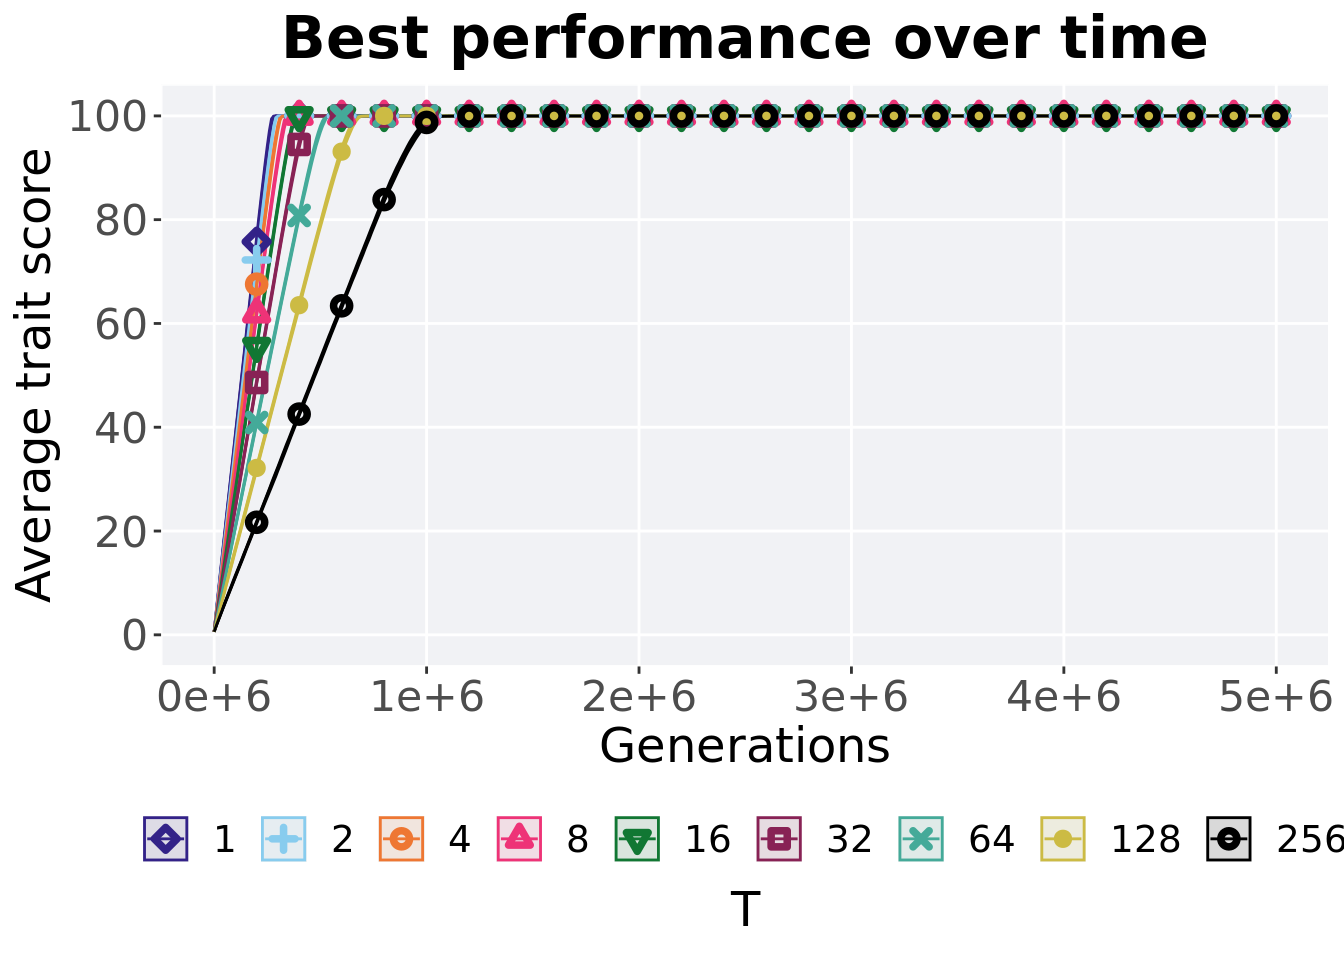
\includegraphics{demo_files/figure-latex/unnamed-chunk-3-1.pdf}

\hypertarget{best-performance-throughout}{%
\section{Best performance throughout}\label{best-performance-throughout}}

Best performance throughout 50,000 generations.

\begin{Shaded}
\begin{Highlighting}[]
\NormalTok{best =}\StringTok{ }\KeywordTok{filter}\NormalTok{(cc_best, col }\OperatorTok{==}\StringTok{ 'pop_fit_max'} \OperatorTok{&}\StringTok{ }\NormalTok{diagnostic }\OperatorTok{==}\StringTok{ 'exploitation_rate'}\NormalTok{)}
\NormalTok{plot =}\StringTok{ }\KeywordTok{ggplot}\NormalTok{(best, }\KeywordTok{aes}\NormalTok{(}\DataTypeTok{x =}\NormalTok{ acron, }\DataTypeTok{y =}\NormalTok{ val }\OperatorTok{/}\StringTok{ }\NormalTok{TRAITS, }\DataTypeTok{color =}\NormalTok{ acron, }\DataTypeTok{fill =}\NormalTok{ acron, }\DataTypeTok{shape =}\NormalTok{ acron)) }\OperatorTok{+}
\StringTok{  }\KeywordTok{geom_flat_violin}\NormalTok{(}\DataTypeTok{position =} \KeywordTok{position_nudge}\NormalTok{(}\DataTypeTok{x =} \FloatTok{.2}\NormalTok{, }\DataTypeTok{y =} \DecValTok{0}\NormalTok{), }\DataTypeTok{scale =} \StringTok{'width'}\NormalTok{, }\DataTypeTok{alpha =} \FloatTok{0.2}\NormalTok{) }\OperatorTok{+}
\StringTok{  }\KeywordTok{geom_point}\NormalTok{(}\DataTypeTok{position =} \KeywordTok{position_jitter}\NormalTok{(}\DataTypeTok{width =} \FloatTok{.1}\NormalTok{), }\DataTypeTok{size =} \FloatTok{1.5}\NormalTok{, }\DataTypeTok{alpha =} \FloatTok{1.0}\NormalTok{) }\OperatorTok{+}
\StringTok{  }\KeywordTok{geom_boxplot}\NormalTok{(}\DataTypeTok{color =} \StringTok{'black'}\NormalTok{, }\DataTypeTok{width =} \FloatTok{.2}\NormalTok{, }\DataTypeTok{outlier.shape =} \OtherTok{NA}\NormalTok{, }\DataTypeTok{alpha =} \FloatTok{0.0}\NormalTok{) }\OperatorTok{+}
\StringTok{  }\KeywordTok{scale_y_continuous}\NormalTok{(}
    \DataTypeTok{name=}\StringTok{"Average trait score"}\NormalTok{,}
    \DataTypeTok{limits=}\KeywordTok{c}\NormalTok{(}\OperatorTok{-}\DecValTok{1}\NormalTok{, }\DecValTok{101}\NormalTok{),}
    \DataTypeTok{breaks=}\KeywordTok{seq}\NormalTok{(}\DecValTok{0}\NormalTok{,}\DecValTok{100}\NormalTok{, }\DecValTok{20}\NormalTok{),}
    \DataTypeTok{labels=}\KeywordTok{c}\NormalTok{(}\StringTok{"0"}\NormalTok{, }\StringTok{"20"}\NormalTok{, }\StringTok{"40"}\NormalTok{, }\StringTok{"60"}\NormalTok{, }\StringTok{"80"}\NormalTok{, }\StringTok{"100"}\NormalTok{)}
\NormalTok{  ) }\OperatorTok{+}
\StringTok{  }\KeywordTok{scale_x_discrete}\NormalTok{(}
    \DataTypeTok{name=}\StringTok{"Scheme"}
\NormalTok{  )}\OperatorTok{+}
\StringTok{  }\KeywordTok{scale_shape_manual}\NormalTok{(}\DataTypeTok{values=}\NormalTok{SHAPE)}\OperatorTok{+}
\StringTok{  }\KeywordTok{scale_colour_manual}\NormalTok{(}\DataTypeTok{values =}\NormalTok{ cb_palette) }\OperatorTok{+}
\StringTok{  }\KeywordTok{scale_fill_manual}\NormalTok{(}\DataTypeTok{values =}\NormalTok{ cb_palette) }\OperatorTok{+}
\StringTok{  }\NormalTok{p_theme}

\KeywordTok{plot_grid}\NormalTok{(}
\NormalTok{  plot }\OperatorTok{+}
\StringTok{    }\KeywordTok{ggtitle}\NormalTok{(}\StringTok{"Best performance throughout"}\NormalTok{) }\OperatorTok{+}
\StringTok{    }\KeywordTok{theme}\NormalTok{(}\DataTypeTok{legend.position=}\StringTok{"none"}\NormalTok{),}
\NormalTok{  legend,}
  \DataTypeTok{nrow=}\DecValTok{2}\NormalTok{,}
  \DataTypeTok{rel_heights =} \KeywordTok{c}\NormalTok{(}\DecValTok{2}\NormalTok{,.}\DecValTok{55}\NormalTok{),}
  \DataTypeTok{label_size =}\NormalTok{ TSIZE}
\NormalTok{)}
\end{Highlighting}
\end{Shaded}

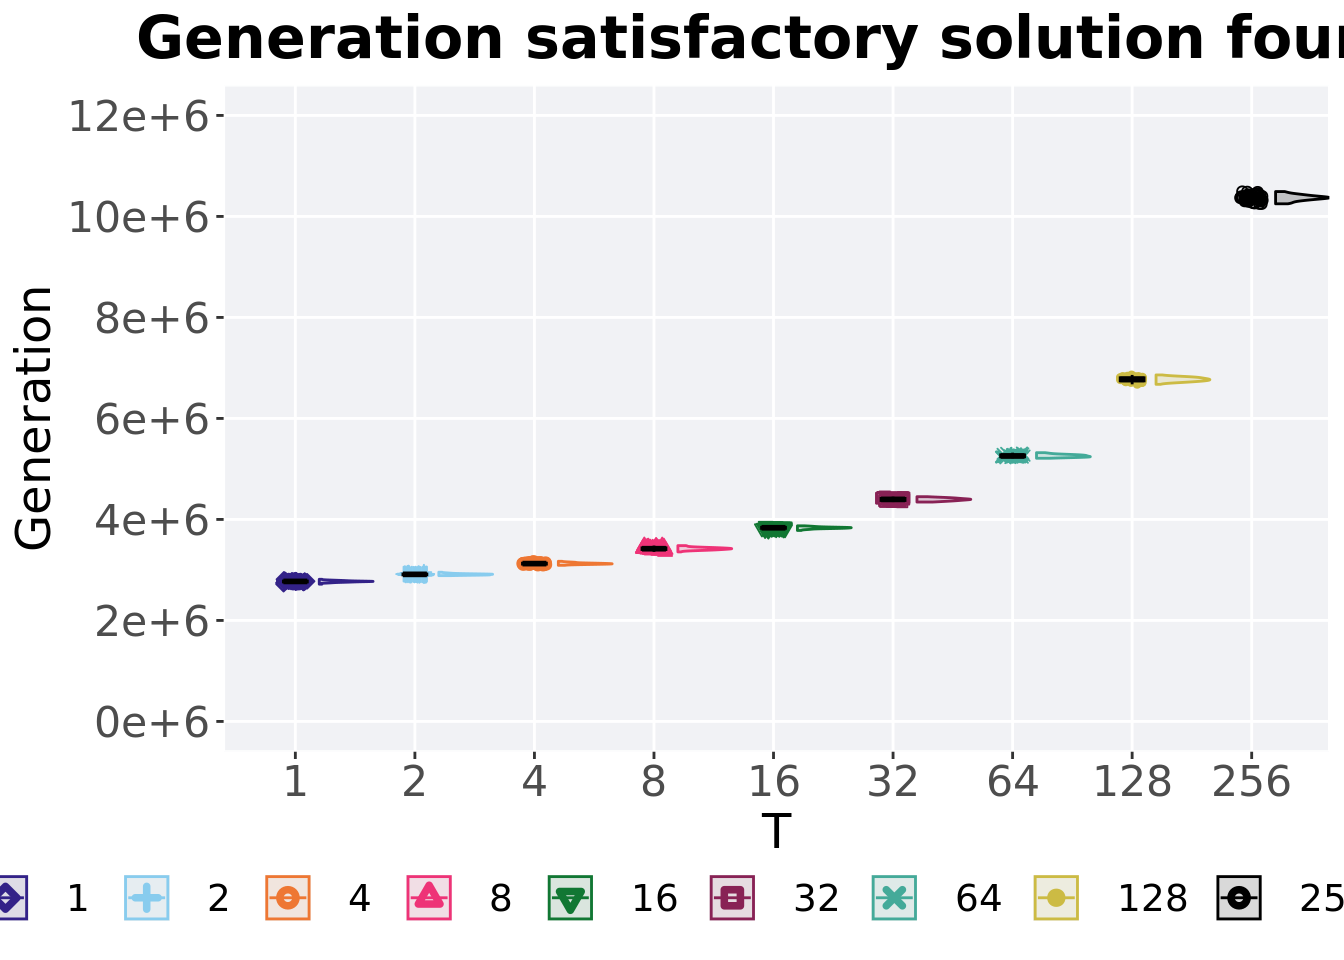
\includegraphics{demo_files/figure-latex/unnamed-chunk-5-1.pdf}

\hypertarget{stats}{%
\subsection{Stats}\label{stats}}

Summary statistics for the performance of the best performance throughout 50,000 generations.

\begin{Shaded}
\begin{Highlighting}[]
\NormalTok{best}\OperatorTok{$}\NormalTok{acron <-}\StringTok{ }\KeywordTok{factor}\NormalTok{(best}\OperatorTok{$}\NormalTok{acron, }\DataTypeTok{levels =} \KeywordTok{c}\NormalTok{(}\StringTok{'tru'}\NormalTok{, }\StringTok{'tor'}\NormalTok{, }\StringTok{'lex'}\NormalTok{,}\StringTok{'nds'}\NormalTok{, }\StringTok{'gfs'}\NormalTok{, }\StringTok{'pfs'}\NormalTok{, }\StringTok{'nov'}\NormalTok{,  }\StringTok{'ran'}\NormalTok{))}
\KeywordTok{group_by}\NormalTok{(best, acron) }\OperatorTok
\StringTok{  }\NormalTok{dplyr}\OperatorTok{::}\KeywordTok{summarise}\NormalTok{(}
    \DataTypeTok{count =} \KeywordTok{n}\NormalTok{(),}
    \DataTypeTok{na_cnt =} \KeywordTok{sum}\NormalTok{(}\KeywordTok{is.na}\NormalTok{(val)),}
    \DataTypeTok{min =} \KeywordTok{min}\NormalTok{(val }\OperatorTok{/}\StringTok{ }\NormalTok{TRAITS, }\DataTypeTok{na.rm =} \OtherTok{TRUE}\NormalTok{),}
    \DataTypeTok{median =} \KeywordTok{median}\NormalTok{(val }\OperatorTok{/}\StringTok{ }\NormalTok{TRAITS, }\DataTypeTok{na.rm =} \OtherTok{TRUE}\NormalTok{),}
    \DataTypeTok{mean =} \KeywordTok{mean}\NormalTok{(val }\OperatorTok{/}\StringTok{ }\NormalTok{TRAITS, }\DataTypeTok{na.rm =} \OtherTok{TRUE}\NormalTok{),}
    \DataTypeTok{max =} \KeywordTok{max}\NormalTok{(val }\OperatorTok{/}\StringTok{ }\NormalTok{TRAITS, }\DataTypeTok{na.rm =} \OtherTok{TRUE}\NormalTok{),}
    \DataTypeTok{IQR =} \KeywordTok{IQR}\NormalTok{(val }\OperatorTok{/}\StringTok{ }\NormalTok{TRAITS, }\DataTypeTok{na.rm =} \OtherTok{TRUE}\NormalTok{)}
\NormalTok{  )}
\end{Highlighting}
\end{Shaded}

\begin{verbatim}
## # A tibble: 8 x 8
##   acron count na_cnt   min median  mean   max    IQR
##   <fct> <int>  <int> <dbl>  <dbl> <dbl> <dbl>  <dbl>
## 1 tru      50      0 100    100   100   100   0     
## 2 tor      50      0 100    100   100   100   0     
## 3 lex      50      0  99.9   99.9  99.9  99.9 0.0183
## 4 nds      50      0  17.3   18.0  18.1  19.4 0.482 
## 5 gfs      50      0  57.8   59.2  59.4  62.4 0.921 
## 6 pfs      50      0  57.5   59.4  59.3  60.7 1.37  
## 7 nov      50      0  15.9   19.1  19.1  23.3 1.50  
## 8 ran      50      0  12.3   15.1  15.2  22.0 2.18
\end{verbatim}

Kruskal--Wallis test provides evidence of statistical differences among best performance found throughout 50,000 generations.

\begin{Shaded}
\begin{Highlighting}[]
\KeywordTok{kruskal.test}\NormalTok{(val }\OperatorTok{~}\StringTok{ }\NormalTok{acron,}\DataTypeTok{data =}\NormalTok{ best)}
\end{Highlighting}
\end{Shaded}

\begin{verbatim}
## 
##  Kruskal-Wallis rank sum test
## 
## data:  val by acron
## Kruskal-Wallis chi-squared = 384.12, df = 7, p-value < 2.2e-16
\end{verbatim}

Results for post-hoc Wilcoxon rank-sum test with a Bonferroni correction on the best performance found throughout 50,000 generations.

\begin{Shaded}
\begin{Highlighting}[]
\KeywordTok{pairwise.wilcox.test}\NormalTok{(}\DataTypeTok{x =}\NormalTok{ best}\OperatorTok{$}\NormalTok{val, }\DataTypeTok{g =}\NormalTok{ best}\OperatorTok{$}\NormalTok{acron, }\DataTypeTok{p.adjust.method =} \StringTok{"bonferroni"}\NormalTok{,}
                     \DataTypeTok{paired =} \OtherTok{FALSE}\NormalTok{, }\DataTypeTok{conf.int =} \OtherTok{FALSE}\NormalTok{, }\DataTypeTok{alternative =} \StringTok{'l'}\NormalTok{)}
\end{Highlighting}
\end{Shaded}

\begin{verbatim}
## 
##  Pairwise comparisons using Wilcoxon rank sum test with continuity correction 
## 
## data:  best$val and best$acron 
## 
##     tru     tor     lex     nds     gfs     pfs     nov    
## tor 1       -       -       -       -       -       -      
## lex < 2e-16 < 2e-16 -       -       -       -       -      
## nds < 2e-16 < 2e-16 < 2e-16 -       -       -       -      
## gfs < 2e-16 < 2e-16 < 2e-16 1       -       -       -      
## pfs < 2e-16 < 2e-16 < 2e-16 1       1       -       -      
## nov < 2e-16 < 2e-16 < 2e-16 1       < 2e-16 < 2e-16 -      
## ran < 2e-16 < 2e-16 < 2e-16 1.3e-14 < 2e-16 < 2e-16 1.6e-14
## 
## P value adjustment method: bonferroni
\end{verbatim}

\hypertarget{generation-satisfactory-solution-found}{%
\section{Generation satisfactory solution found}\label{generation-satisfactory-solution-found}}

First generation a satisfactory solution is found throughout the 50,000 generations.

\begin{Shaded}
\begin{Highlighting}[]
\NormalTok{ssf =}\StringTok{ }\KeywordTok{filter}\NormalTok{(cc_ssf, diagnostic }\OperatorTok{==}\StringTok{ 'exploitation_rate'}\NormalTok{)}
\NormalTok{schemes =}\StringTok{ }\KeywordTok{data.frame}\NormalTok{()}

\ControlFlowTok{for}\NormalTok{ (i }\ControlFlowTok{in} \DecValTok{1}\OperatorTok{:}\DecValTok{8}\NormalTok{) \{}
  \ControlFlowTok{if}\NormalTok{(i }\OperatorTok{==}\StringTok{ }\DecValTok{5}\NormalTok{)}
\NormalTok{  \{}
\NormalTok{    schemes =}\StringTok{ }\KeywordTok{rbind}\NormalTok{(schemes, }\KeywordTok{filter}\NormalTok{(ssf, acron }\OperatorTok{==}\StringTok{ }\NormalTok{ACRON[i]))}
    \ControlFlowTok{next}
\NormalTok{  \}}
\NormalTok{  schemes =}\StringTok{ }\KeywordTok{rbind}\NormalTok{(schemes, }\KeywordTok{filter}\NormalTok{(ssf, acron }\OperatorTok{==}\StringTok{ }\NormalTok{ACRON[i] }\OperatorTok{&}\StringTok{ }\NormalTok{trt }\OperatorTok{==}\StringTok{ }\NormalTok{PARAM[i]))}
\NormalTok{\}}

\NormalTok{plot <-}\StringTok{ }\KeywordTok{ggplot}\NormalTok{(schemes, }\KeywordTok{aes}\NormalTok{(}\DataTypeTok{x =}\NormalTok{ acron, }\DataTypeTok{y =}\NormalTok{ generation, }\DataTypeTok{color =}\NormalTok{ acron, }\DataTypeTok{fill =}\NormalTok{ acron, }\DataTypeTok{shape =}\NormalTok{ acron)) }\OperatorTok{+}
\StringTok{  }\KeywordTok{geom_flat_violin}\NormalTok{(}\DataTypeTok{position =} \KeywordTok{position_nudge}\NormalTok{(}\DataTypeTok{x =} \FloatTok{.2}\NormalTok{, }\DataTypeTok{y =} \DecValTok{0}\NormalTok{), }\DataTypeTok{scale =} \StringTok{'width'}\NormalTok{, }\DataTypeTok{alpha =} \FloatTok{0.2}\NormalTok{) }\OperatorTok{+}
\StringTok{  }\KeywordTok{geom_point}\NormalTok{(}\DataTypeTok{position =} \KeywordTok{position_jitter}\NormalTok{(}\DataTypeTok{width =} \FloatTok{.1}\NormalTok{), }\DataTypeTok{size =} \FloatTok{1.5}\NormalTok{, }\DataTypeTok{alpha =} \FloatTok{1.0}\NormalTok{) }\OperatorTok{+}
\StringTok{  }\KeywordTok{geom_boxplot}\NormalTok{(}\DataTypeTok{color =} \StringTok{'black'}\NormalTok{, }\DataTypeTok{width =} \FloatTok{.2}\NormalTok{, }\DataTypeTok{outlier.shape =} \OtherTok{NA}\NormalTok{, }\DataTypeTok{alpha =} \FloatTok{0.0}\NormalTok{) }\OperatorTok{+}
\StringTok{  }\KeywordTok{scale_shape_manual}\NormalTok{(}\DataTypeTok{values=}\NormalTok{SHAPE)}\OperatorTok{+}
\StringTok{  }\KeywordTok{scale_y_continuous}\NormalTok{(}
    \DataTypeTok{name=}\StringTok{"Generation"}\NormalTok{,}
    \DataTypeTok{limits=}\KeywordTok{c}\NormalTok{(}\DecValTok{0}\NormalTok{, }\DecValTok{60000}\NormalTok{),}
    \DataTypeTok{breaks=}\KeywordTok{c}\NormalTok{(}\DecValTok{0}\NormalTok{, }\DecValTok{10000}\NormalTok{, }\DecValTok{20000}\NormalTok{, }\DecValTok{30000}\NormalTok{, }\DecValTok{40000}\NormalTok{, }\DecValTok{50000}\NormalTok{, }\DecValTok{60000}\NormalTok{),}
    \DataTypeTok{labels=}\KeywordTok{c}\NormalTok{(}\StringTok{"0e+6"}\NormalTok{, }\StringTok{"1e+6"}\NormalTok{, }\StringTok{"2e+6"}\NormalTok{, }\StringTok{"3e+6"}\NormalTok{, }\StringTok{"4e+6"}\NormalTok{, }\StringTok{"5e+6"}\NormalTok{, }\StringTok{"Fail"}\NormalTok{)}
\NormalTok{  ) }\OperatorTok{+}
\StringTok{  }\KeywordTok{scale_x_discrete}\NormalTok{(}
    \DataTypeTok{name=}\StringTok{"Scheme"}
\NormalTok{  ) }\OperatorTok{+}
\StringTok{  }\KeywordTok{scale_colour_manual}\NormalTok{(}\DataTypeTok{values =}\NormalTok{ cb_palette) }\OperatorTok{+}
\StringTok{  }\KeywordTok{scale_fill_manual}\NormalTok{(}\DataTypeTok{values =}\NormalTok{ cb_palette) }\OperatorTok{+}
\StringTok{  }\NormalTok{p_theme}

\KeywordTok{plot_grid}\NormalTok{(}
\NormalTok{  plot }\OperatorTok{+}
\StringTok{    }\KeywordTok{ggtitle}\NormalTok{(}\StringTok{"Generation satisfactory solution found"}\NormalTok{) }\OperatorTok{+}
\StringTok{    }\KeywordTok{theme}\NormalTok{(}\DataTypeTok{legend.position=}\StringTok{"none"}\NormalTok{),}
\NormalTok{  legend,}
  \DataTypeTok{nrow=}\DecValTok{2}\NormalTok{,}
  \DataTypeTok{rel_heights =} \KeywordTok{c}\NormalTok{(}\DecValTok{2}\NormalTok{,.}\DecValTok{55}\NormalTok{),}
  \DataTypeTok{label_size =}\NormalTok{ TSIZE}
\NormalTok{)}
\end{Highlighting}
\end{Shaded}

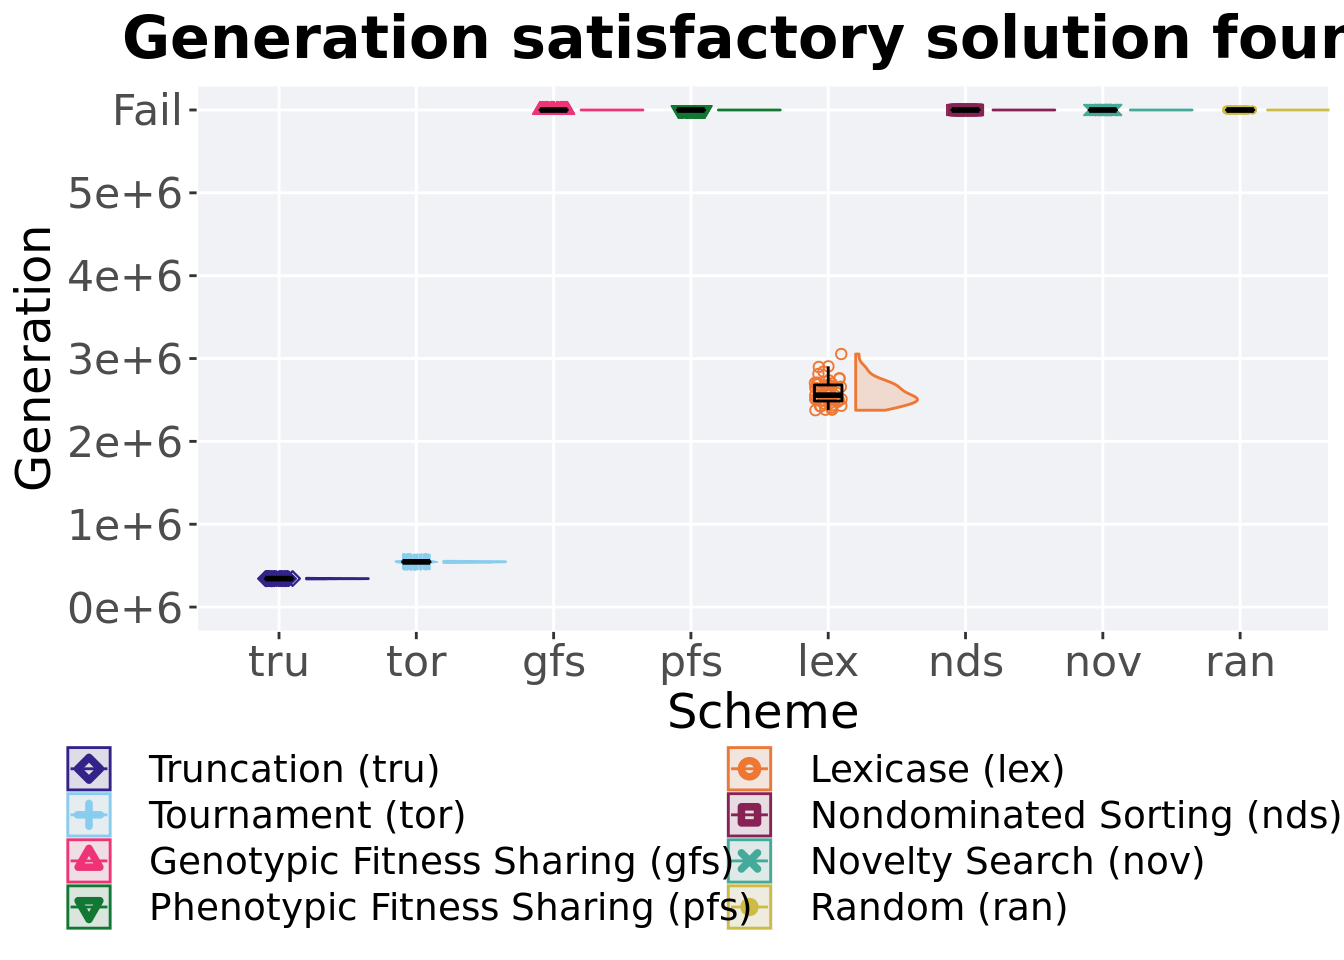
\includegraphics{demo_files/figure-latex/unnamed-chunk-9-1.pdf}

\hypertarget{stats-1}{%
\subsection{Stats}\label{stats-1}}

Summary statistics for the first generation a satisfactory solution is found throughout the 50,000 generations.

\begin{Shaded}
\begin{Highlighting}[]
\NormalTok{schemes <-}\StringTok{ }\KeywordTok{filter}\NormalTok{(schemes, acron }\OperatorTok{==}\StringTok{ 'tru'} \OperatorTok{|}\StringTok{ }\NormalTok{acron }\OperatorTok{==}\StringTok{ 'tor'} \OperatorTok{|}\StringTok{ }\NormalTok{acron }\OperatorTok{==}\StringTok{ 'lex'}\NormalTok{)}
\KeywordTok{group_by}\NormalTok{(schemes, acron) }\OperatorTok
\StringTok{  }\NormalTok{dplyr}\OperatorTok{::}\KeywordTok{summarise}\NormalTok{(}
    \DataTypeTok{count =} \KeywordTok{n}\NormalTok{(),}
    \DataTypeTok{na_cnt =} \KeywordTok{sum}\NormalTok{(}\KeywordTok{is.na}\NormalTok{(generation)),}
    \DataTypeTok{min =} \KeywordTok{min}\NormalTok{(generation, }\DataTypeTok{na.rm =} \OtherTok{TRUE}\NormalTok{),}
    \DataTypeTok{median =} \KeywordTok{median}\NormalTok{(generation, }\DataTypeTok{na.rm =} \OtherTok{TRUE}\NormalTok{),}
    \DataTypeTok{mean =} \KeywordTok{mean}\NormalTok{(generation, }\DataTypeTok{na.rm =} \OtherTok{TRUE}\NormalTok{),}
    \DataTypeTok{max =} \KeywordTok{max}\NormalTok{(generation, }\DataTypeTok{na.rm =} \OtherTok{TRUE}\NormalTok{),}
    \DataTypeTok{IQR =} \KeywordTok{IQR}\NormalTok{(generation, }\DataTypeTok{na.rm =} \OtherTok{TRUE}\NormalTok{)}
\NormalTok{  )}
\end{Highlighting}
\end{Shaded}

\begin{verbatim}
## # A tibble: 3 x 8
##   acron count na_cnt   min median   mean   max   IQR
##   <fct> <int>  <int> <dbl>  <dbl>  <dbl> <dbl> <dbl>
## 1 tru      50      0  3399  3430.  3432.  3478    18
## 2 tor      50      0  5379  5457   5453.  5529    56
## 3 lex      50      0 23761 25580. 25863. 30542  1935
\end{verbatim}

Kruskal--Wallis test provides evidence of difference amoung selection schemes the first generation a satisfactory solution is found throughout the 50,000 generations.

\begin{Shaded}
\begin{Highlighting}[]
\KeywordTok{kruskal.test}\NormalTok{(generation }\OperatorTok{~}\StringTok{ }\NormalTok{acron, }\DataTypeTok{data =}\NormalTok{ schemes)}
\end{Highlighting}
\end{Shaded}

\begin{verbatim}
## 
##  Kruskal-Wallis rank sum test
## 
## data:  generation by acron
## Kruskal-Wallis chi-squared = 132.46, df = 2, p-value < 2.2e-16
\end{verbatim}

Results for post-hoc Wilcoxon rank-sum test with a Bonferroni correction on the first generation a satisfactory solution is found throughout the 50,000 generations.

\begin{Shaded}
\begin{Highlighting}[]
\KeywordTok{pairwise.wilcox.test}\NormalTok{(}\DataTypeTok{x =}\NormalTok{ schemes}\OperatorTok{$}\NormalTok{generation, }\DataTypeTok{g =}\NormalTok{ schemes}\OperatorTok{$}\NormalTok{acron, }\DataTypeTok{p.adjust.method =} \StringTok{"bonferroni"}\NormalTok{,}
                     \DataTypeTok{paired =} \OtherTok{FALSE}\NormalTok{, }\DataTypeTok{conf.int =} \OtherTok{FALSE}\NormalTok{, }\DataTypeTok{alternative =} \StringTok{'g'}\NormalTok{)}
\end{Highlighting}
\end{Shaded}

\begin{verbatim}
## 
##  Pairwise comparisons using Wilcoxon rank sum test with continuity correction 
## 
## data:  schemes$generation and schemes$acron 
## 
##     tru    tor   
## tor <2e-16 -     
## lex <2e-16 <2e-16
## 
## P value adjustment method: bonferroni
\end{verbatim}

\hypertarget{ordered-exploitation-results}{%
\chapter{Ordered exploitation results}\label{ordered-exploitation-results}}

Here we present the results for \textbf{best performances} found by each selection scheme replicate on the exploitation rate diagnostic.
Best performance found refers to the largest average trait score found in a given population.
Note that performance values fall between 0 and 100.

\hypertarget{analysis-dependencies-1}{%
\section{Analysis dependencies}\label{analysis-dependencies-1}}

\begin{Shaded}
\begin{Highlighting}[]
\KeywordTok{library}\NormalTok{(ggplot2)}
\KeywordTok{library}\NormalTok{(cowplot)}
\KeywordTok{library}\NormalTok{(dplyr)}
\KeywordTok{library}\NormalTok{(PupillometryR)}
\end{Highlighting}
\end{Shaded}

\hypertarget{setup-1}{%
\section{Setup}\label{setup-1}}

These analyses were conducted in the following computing environment:

\begin{Shaded}
\begin{Highlighting}[]
\KeywordTok{print}\NormalTok{(version)}
\end{Highlighting}
\end{Shaded}

\begin{verbatim}
##                _                           
## platform       x86_64-pc-linux-gnu         
## arch           x86_64                      
## os             linux-gnu                   
## system         x86_64, linux-gnu           
## status                                     
## major          4                           
## minor          2.1                         
## year           2022                        
## month          06                          
## day            23                          
## svn rev        82513                       
## language       R                           
## version.string R version 4.2.1 (2022-06-23)
## nickname       Funny-Looking Kid
\end{verbatim}

\hypertarget{performance-over-time-1}{%
\section{Performance over time}\label{performance-over-time-1}}

Best performance in a population over time.

\begin{Shaded}
\begin{Highlighting}[]
\NormalTok{ordered_exploitation =}\StringTok{ }\KeywordTok{filter}\NormalTok{(cc_over_time, diagnostic }\OperatorTok{==}\StringTok{ 'ordered_exploitation'}\NormalTok{)}
\NormalTok{lines =}\StringTok{ }\NormalTok{ordered_exploitation }\OperatorTok
\StringTok{        }\KeywordTok{group_by}\NormalTok{(}\StringTok{`}\DataTypeTok{Selection}\CharTok{\textbackslash{}n}\DataTypeTok{Scheme}\StringTok{`}\NormalTok{, gen) }\OperatorTok
\StringTok{          }\NormalTok{dplyr}\OperatorTok{::}\KeywordTok{summarise}\NormalTok{(}
            \DataTypeTok{min =} \KeywordTok{min}\NormalTok{(pop_fit_max),}
            \DataTypeTok{mean =} \KeywordTok{mean}\NormalTok{(pop_fit_max),}
            \DataTypeTok{max =} \KeywordTok{max}\NormalTok{(pop_fit_max)}
\NormalTok{          )}
\end{Highlighting}
\end{Shaded}

\begin{verbatim}
## `summarise()` has grouped output by 'Selection Scheme'. You can override using
## the `.groups` argument.
\end{verbatim}

\begin{Shaded}
\begin{Highlighting}[]
\NormalTok{points =}\StringTok{ }\KeywordTok{filter}\NormalTok{(lines, gen }\OperatorTok\StringTok{ }\DecValTok{2000} \OperatorTok{==}\StringTok{ }\DecValTok{0} \OperatorTok{&}\StringTok{ }\NormalTok{gen }\OperatorTok{!=}\StringTok{ }\DecValTok{0}\NormalTok{)}

\NormalTok{ot =}\StringTok{ }\KeywordTok{ggplot}\NormalTok{(lines, }\KeywordTok{aes}\NormalTok{(}\DataTypeTok{x=}\NormalTok{gen, }\DataTypeTok{y=}\NormalTok{mean }\OperatorTok{/}\StringTok{ }\NormalTok{TRAITS, }\DataTypeTok{group =} \StringTok{`}\DataTypeTok{Selection}\CharTok{\textbackslash{}n}\DataTypeTok{Scheme}\StringTok{`}\NormalTok{, }\DataTypeTok{fill =}\StringTok{`}\DataTypeTok{Selection}\CharTok{\textbackslash{}n}\DataTypeTok{Scheme}\StringTok{`}\NormalTok{, }\DataTypeTok{color =} \StringTok{`}\DataTypeTok{Selection}\CharTok{\textbackslash{}n}\DataTypeTok{Scheme}\StringTok{`}\NormalTok{, }\DataTypeTok{shape =} \StringTok{`}\DataTypeTok{Selection}\CharTok{\textbackslash{}n}\DataTypeTok{Scheme}\StringTok{`}\NormalTok{)) }\OperatorTok{+}
\StringTok{  }\KeywordTok{geom_ribbon}\NormalTok{(}\KeywordTok{aes}\NormalTok{(}\DataTypeTok{ymin =}\NormalTok{ min }\OperatorTok{/}\StringTok{ }\NormalTok{TRAITS, }\DataTypeTok{ymax =}\NormalTok{ max }\OperatorTok{/}\StringTok{ }\NormalTok{TRAITS), }\DataTypeTok{alpha =} \FloatTok{0.1}\NormalTok{) }\OperatorTok{+}
\StringTok{  }\KeywordTok{geom_line}\NormalTok{(}\DataTypeTok{size =} \FloatTok{0.5}\NormalTok{) }\OperatorTok{+}
\StringTok{  }\KeywordTok{geom_point}\NormalTok{(}\DataTypeTok{data =}\NormalTok{ points, }\DataTypeTok{size =} \FloatTok{1.5}\NormalTok{, }\DataTypeTok{stroke =} \FloatTok{2.0}\NormalTok{, }\DataTypeTok{alpha =} \FloatTok{1.0}\NormalTok{) }\OperatorTok{+}
\StringTok{  }\KeywordTok{scale_y_continuous}\NormalTok{(}
    \DataTypeTok{name=}\StringTok{"Average trait score"}\NormalTok{,}
    \DataTypeTok{limits=}\KeywordTok{c}\NormalTok{(}\OperatorTok{-}\DecValTok{1}\NormalTok{, }\DecValTok{101}\NormalTok{),}
    \DataTypeTok{breaks=}\KeywordTok{seq}\NormalTok{(}\DecValTok{0}\NormalTok{,}\DecValTok{100}\NormalTok{, }\DecValTok{20}\NormalTok{),}
    \DataTypeTok{labels=}\KeywordTok{c}\NormalTok{(}\StringTok{"0"}\NormalTok{, }\StringTok{"20"}\NormalTok{, }\StringTok{"40"}\NormalTok{, }\StringTok{"60"}\NormalTok{, }\StringTok{"80"}\NormalTok{, }\StringTok{"100"}\NormalTok{)}
\NormalTok{  ) }\OperatorTok{+}
\StringTok{  }\KeywordTok{scale_x_continuous}\NormalTok{(}
    \DataTypeTok{name=}\StringTok{"Generations"}\NormalTok{,}
    \DataTypeTok{limits=}\KeywordTok{c}\NormalTok{(}\DecValTok{0}\NormalTok{, }\DecValTok{50000}\NormalTok{),}
    \DataTypeTok{breaks=}\KeywordTok{c}\NormalTok{(}\DecValTok{0}\NormalTok{, }\DecValTok{10000}\NormalTok{, }\DecValTok{20000}\NormalTok{, }\DecValTok{30000}\NormalTok{, }\DecValTok{40000}\NormalTok{, }\DecValTok{50000}\NormalTok{),}
    \DataTypeTok{labels=}\KeywordTok{c}\NormalTok{(}\StringTok{"0e+6"}\NormalTok{, }\StringTok{"1e+6"}\NormalTok{, }\StringTok{"2e+6"}\NormalTok{, }\StringTok{"3e+6"}\NormalTok{, }\StringTok{"4e+6"}\NormalTok{, }\StringTok{"5e+6"}\NormalTok{)}

\NormalTok{  ) }\OperatorTok{+}
\StringTok{  }\KeywordTok{scale_shape_manual}\NormalTok{(}\DataTypeTok{values=}\NormalTok{SHAPE)}\OperatorTok{+}
\StringTok{  }\KeywordTok{scale_colour_manual}\NormalTok{(}\DataTypeTok{values =}\NormalTok{ cb_palette) }\OperatorTok{+}
\StringTok{  }\KeywordTok{scale_fill_manual}\NormalTok{(}\DataTypeTok{values =}\NormalTok{ cb_palette) }\OperatorTok{+}
\StringTok{  }\KeywordTok{ggtitle}\NormalTok{(}\StringTok{"Best performance over time"}\NormalTok{) }\OperatorTok{+}
\StringTok{  }\NormalTok{p_theme}\OperatorTok{+}
\StringTok{    }\KeywordTok{guides}\NormalTok{(}
    \DataTypeTok{shape=}\KeywordTok{guide_legend}\NormalTok{(}\DataTypeTok{ncol=}\DecValTok{2}\NormalTok{, }\DataTypeTok{title.position =} \StringTok{"bottom"}\NormalTok{),}
    \DataTypeTok{color=}\KeywordTok{guide_legend}\NormalTok{(}\DataTypeTok{ncol=}\DecValTok{2}\NormalTok{, }\DataTypeTok{title.position =} \StringTok{"bottom"}\NormalTok{),}
    \DataTypeTok{fill=}\KeywordTok{guide_legend}\NormalTok{(}\DataTypeTok{ncol=}\DecValTok{2}\NormalTok{, }\DataTypeTok{title.position =} \StringTok{"bottom"}\NormalTok{)}
\NormalTok{  ) }\OperatorTok{+}
\StringTok{  }\KeywordTok{theme}\NormalTok{(}
    \DataTypeTok{legend.position =} \StringTok{"bottom"}\NormalTok{,}
    \DataTypeTok{legend.box=}\StringTok{"verticle"}\NormalTok{,}
    \DataTypeTok{legend.justification=}\StringTok{"center"}\NormalTok{,}
    \DataTypeTok{legend.title=}\KeywordTok{element_blank}\NormalTok{()}
\NormalTok{  )}

\NormalTok{ot}
\end{Highlighting}
\end{Shaded}

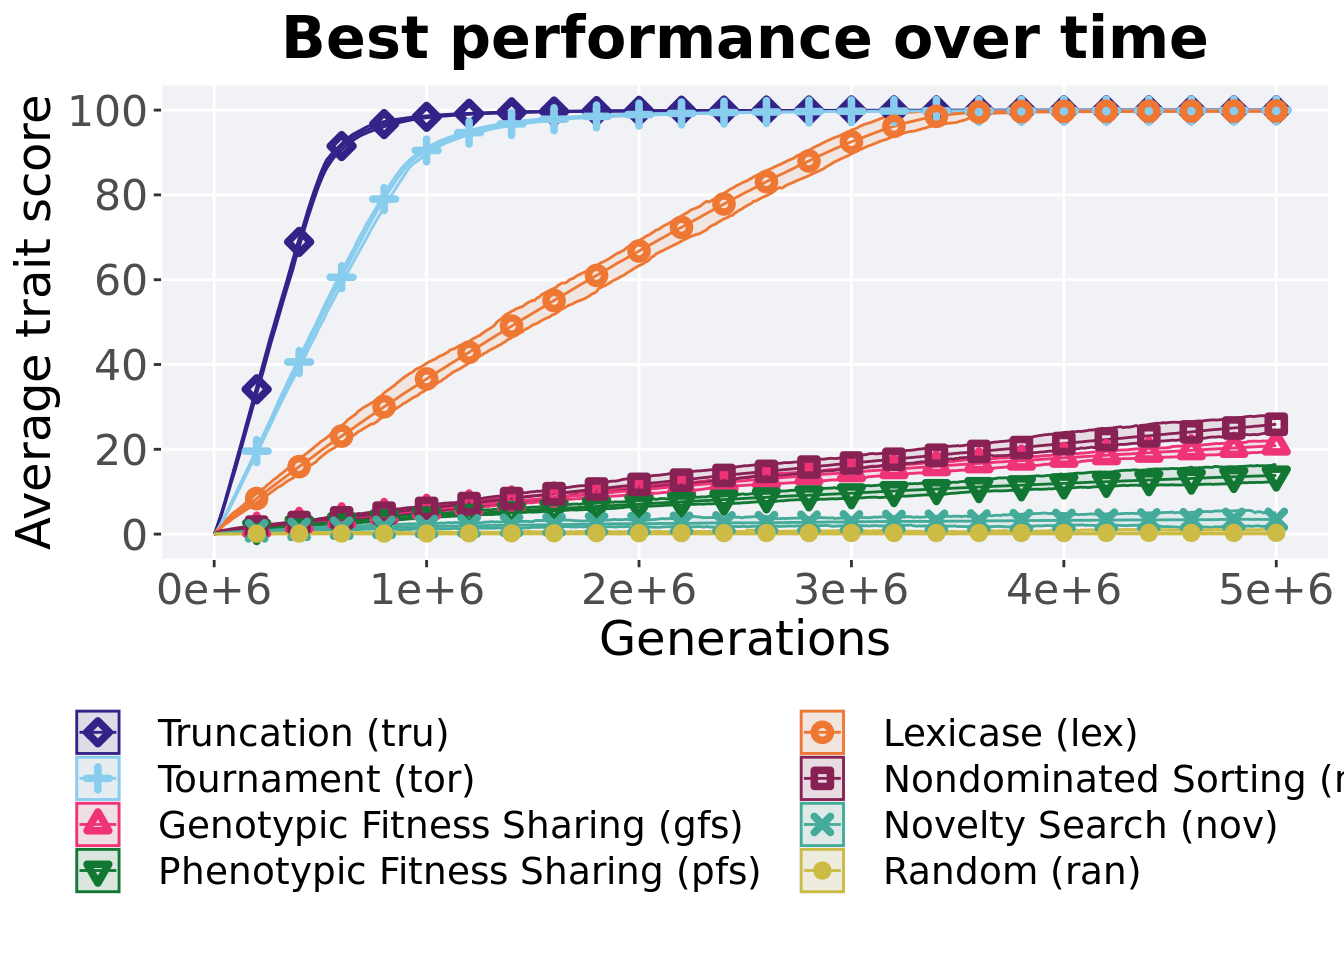
\includegraphics{demo_files/figure-latex/unnamed-chunk-15-1.pdf}

\hypertarget{best-performance-throughout-1}{%
\section{Best performance throughout}\label{best-performance-throughout-1}}

Best performance throughout 50,000 generations.

\begin{Shaded}
\begin{Highlighting}[]
\NormalTok{best =}\StringTok{ }\KeywordTok{filter}\NormalTok{(cc_best, col }\OperatorTok{==}\StringTok{ 'pop_fit_max'} \OperatorTok{&}\StringTok{ }\NormalTok{diagnostic }\OperatorTok{==}\StringTok{ 'ordered_exploitation'}\NormalTok{)}
\NormalTok{plot =}\StringTok{ }\KeywordTok{ggplot}\NormalTok{(best, }\KeywordTok{aes}\NormalTok{(}\DataTypeTok{x =}\NormalTok{ acron, }\DataTypeTok{y =}\NormalTok{ val }\OperatorTok{/}\StringTok{ }\NormalTok{TRAITS, }\DataTypeTok{color =}\NormalTok{ acron, }\DataTypeTok{fill =}\NormalTok{ acron, }\DataTypeTok{shape =}\NormalTok{ acron)) }\OperatorTok{+}
\StringTok{  }\KeywordTok{geom_flat_violin}\NormalTok{(}\DataTypeTok{position =} \KeywordTok{position_nudge}\NormalTok{(}\DataTypeTok{x =} \FloatTok{.2}\NormalTok{, }\DataTypeTok{y =} \DecValTok{0}\NormalTok{), }\DataTypeTok{scale =} \StringTok{'width'}\NormalTok{, }\DataTypeTok{alpha =} \FloatTok{0.2}\NormalTok{) }\OperatorTok{+}
\StringTok{  }\KeywordTok{geom_point}\NormalTok{(}\DataTypeTok{position =} \KeywordTok{position_jitter}\NormalTok{(}\DataTypeTok{width =} \FloatTok{.1}\NormalTok{), }\DataTypeTok{size =} \FloatTok{1.5}\NormalTok{, }\DataTypeTok{alpha =} \FloatTok{1.0}\NormalTok{) }\OperatorTok{+}
\StringTok{  }\KeywordTok{geom_boxplot}\NormalTok{(}\DataTypeTok{color =} \StringTok{'black'}\NormalTok{, }\DataTypeTok{width =} \FloatTok{.2}\NormalTok{, }\DataTypeTok{outlier.shape =} \OtherTok{NA}\NormalTok{, }\DataTypeTok{alpha =} \FloatTok{0.0}\NormalTok{) }\OperatorTok{+}
\StringTok{  }\KeywordTok{scale_y_continuous}\NormalTok{(}
    \DataTypeTok{name=}\StringTok{"Average trait score"}\NormalTok{,}
    \DataTypeTok{limits=}\KeywordTok{c}\NormalTok{(}\OperatorTok{-}\DecValTok{1}\NormalTok{, }\DecValTok{101}\NormalTok{),}
    \DataTypeTok{breaks=}\KeywordTok{seq}\NormalTok{(}\DecValTok{0}\NormalTok{,}\DecValTok{100}\NormalTok{, }\DecValTok{20}\NormalTok{),}
    \DataTypeTok{labels=}\KeywordTok{c}\NormalTok{(}\StringTok{"0"}\NormalTok{, }\StringTok{"20"}\NormalTok{, }\StringTok{"40"}\NormalTok{, }\StringTok{"60"}\NormalTok{, }\StringTok{"80"}\NormalTok{, }\StringTok{"100"}\NormalTok{)}
\NormalTok{  ) }\OperatorTok{+}
\StringTok{  }\KeywordTok{scale_x_discrete}\NormalTok{(}
    \DataTypeTok{name=}\StringTok{"Scheme"}
\NormalTok{  )}\OperatorTok{+}
\StringTok{  }\KeywordTok{scale_shape_manual}\NormalTok{(}\DataTypeTok{values=}\NormalTok{SHAPE)}\OperatorTok{+}
\StringTok{  }\KeywordTok{scale_colour_manual}\NormalTok{(}\DataTypeTok{values =}\NormalTok{ cb_palette) }\OperatorTok{+}
\StringTok{  }\KeywordTok{scale_fill_manual}\NormalTok{(}\DataTypeTok{values =}\NormalTok{ cb_palette) }\OperatorTok{+}
\StringTok{  }\NormalTok{p_theme}

\KeywordTok{plot_grid}\NormalTok{(}
\NormalTok{  plot }\OperatorTok{+}
\StringTok{    }\KeywordTok{ggtitle}\NormalTok{(}\StringTok{"Best performance throughout"}\NormalTok{) }\OperatorTok{+}
\StringTok{    }\KeywordTok{theme}\NormalTok{(}\DataTypeTok{legend.position=}\StringTok{"none"}\NormalTok{),}
\NormalTok{  legend,}
  \DataTypeTok{nrow=}\DecValTok{2}\NormalTok{,}
  \DataTypeTok{rel_heights =} \KeywordTok{c}\NormalTok{(}\DecValTok{2}\NormalTok{,.}\DecValTok{55}\NormalTok{),}
  \DataTypeTok{label_size =}\NormalTok{ TSIZE}
\NormalTok{)}
\end{Highlighting}
\end{Shaded}

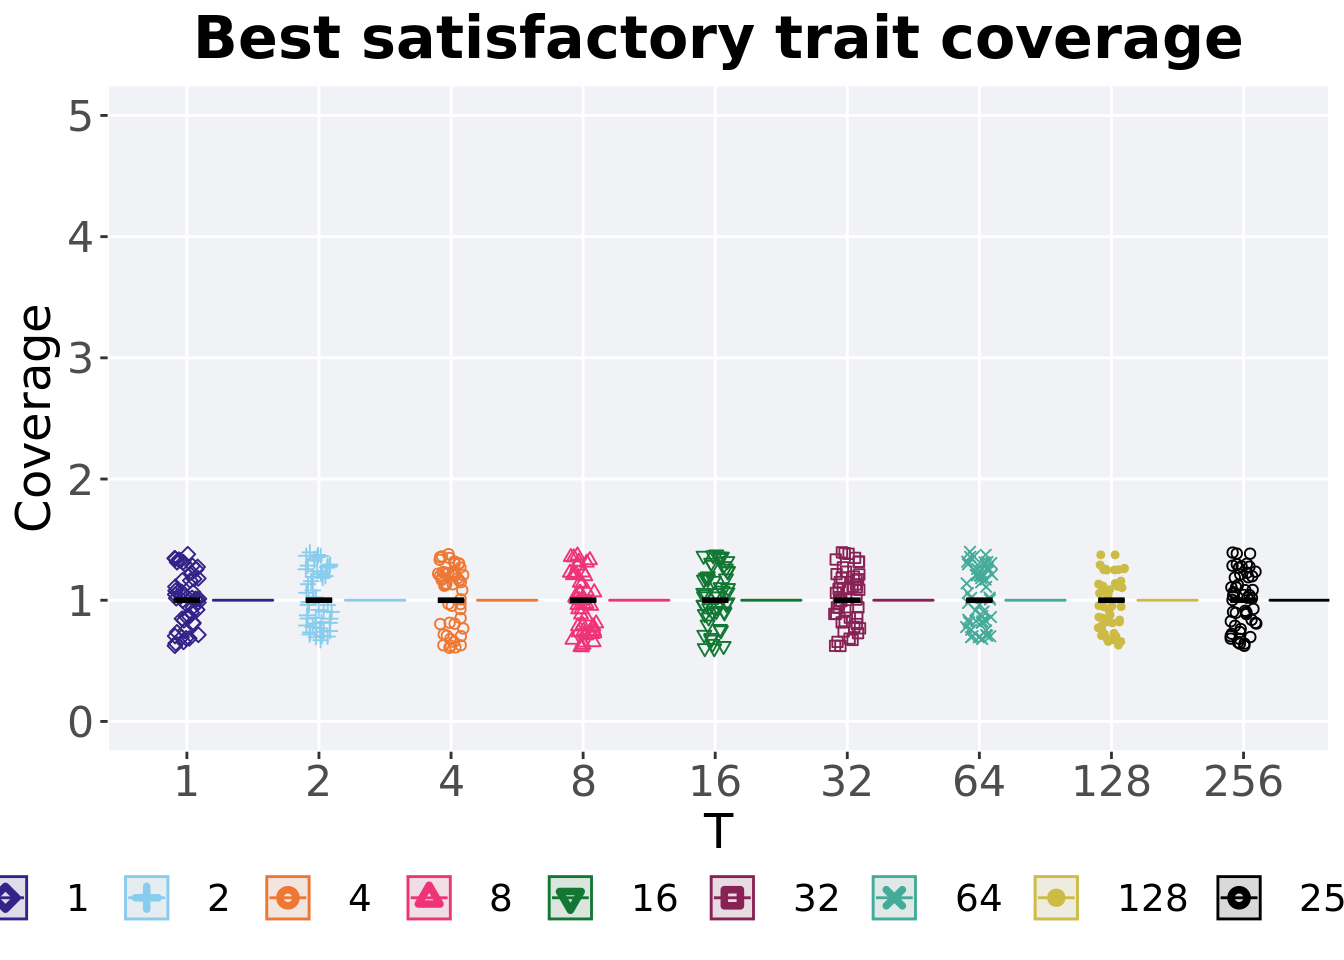
\includegraphics{demo_files/figure-latex/unnamed-chunk-17-1.pdf}

\hypertarget{stats-2}{%
\subsection{Stats}\label{stats-2}}

Summary statistics for the performance of the best performance throughout 50,000 generations.

\begin{Shaded}
\begin{Highlighting}[]
\NormalTok{best}\OperatorTok{$}\NormalTok{acron <-}\StringTok{ }\KeywordTok{factor}\NormalTok{(best}\OperatorTok{$}\NormalTok{acron, }\DataTypeTok{levels =} \KeywordTok{c}\NormalTok{(}\StringTok{'tru'}\NormalTok{, }\StringTok{'tor'}\NormalTok{, }\StringTok{'lex'}\NormalTok{,}\StringTok{'nds'}\NormalTok{, }\StringTok{'gfs'}\NormalTok{, }\StringTok{'pfs'}\NormalTok{, }\StringTok{'nov'}\NormalTok{,  }\StringTok{'ran'}\NormalTok{))}
\KeywordTok{group_by}\NormalTok{(best, acron) }\OperatorTok
\StringTok{  }\NormalTok{dplyr}\OperatorTok{::}\KeywordTok{summarise}\NormalTok{(}
    \DataTypeTok{count =} \KeywordTok{n}\NormalTok{(),}
    \DataTypeTok{na_cnt =} \KeywordTok{sum}\NormalTok{(}\KeywordTok{is.na}\NormalTok{(val)),}
    \DataTypeTok{min =} \KeywordTok{min}\NormalTok{(val }\OperatorTok{/}\StringTok{ }\NormalTok{TRAITS, }\DataTypeTok{na.rm =} \OtherTok{TRUE}\NormalTok{),}
    \DataTypeTok{median =} \KeywordTok{median}\NormalTok{(val }\OperatorTok{/}\StringTok{ }\NormalTok{TRAITS, }\DataTypeTok{na.rm =} \OtherTok{TRUE}\NormalTok{),}
    \DataTypeTok{mean =} \KeywordTok{mean}\NormalTok{(val }\OperatorTok{/}\StringTok{ }\NormalTok{TRAITS, }\DataTypeTok{na.rm =} \OtherTok{TRUE}\NormalTok{),}
    \DataTypeTok{max =} \KeywordTok{max}\NormalTok{(val }\OperatorTok{/}\StringTok{ }\NormalTok{TRAITS, }\DataTypeTok{na.rm =} \OtherTok{TRUE}\NormalTok{),}
    \DataTypeTok{IQR =} \KeywordTok{IQR}\NormalTok{(val }\OperatorTok{/}\StringTok{ }\NormalTok{TRAITS, }\DataTypeTok{na.rm =} \OtherTok{TRUE}\NormalTok{)}
\NormalTok{  )}
\end{Highlighting}
\end{Shaded}

\begin{verbatim}
## # A tibble: 8 x 8
##   acron count na_cnt     min  median    mean    max     IQR
##   <fct> <int>  <int>   <dbl>   <dbl>   <dbl>  <dbl>   <dbl>
## 1 tru      50      0 100.    100.    100.    100.   0.00225
## 2 tor      50      0  99.9    99.9    99.9    99.9  0.00540
## 3 lex      50      0  99.7    99.8    99.8    99.8  0.0239 
## 4 nds      50      0  24.1    26.0    26.0    28.1  1.04   
## 5 gfs      50      0  19.6    21.0    20.9    22.1  0.686  
## 6 pfs      50      0  12.5    13.9    13.9    16.4  1.21   
## 7 nov      50      0   2.70    3.88    3.89    5.62 0.846  
## 8 ran      50      0   0.310   0.594   0.640   1.23 0.317
\end{verbatim}

Kruskal--Wallis test provides evidence of statistical differences among best performance found throughout 50,000 generations.

\begin{Shaded}
\begin{Highlighting}[]
\KeywordTok{kruskal.test}\NormalTok{(val }\OperatorTok{~}\StringTok{ }\NormalTok{acron,}\DataTypeTok{data =}\NormalTok{ best)}
\end{Highlighting}
\end{Shaded}

\begin{verbatim}
## 
##  Kruskal-Wallis rank sum test
## 
## data:  val by acron
## Kruskal-Wallis chi-squared = 392.77, df = 7, p-value < 2.2e-16
\end{verbatim}

Results for post-hoc Wilcoxon rank-sum test with a Bonferroni correction on the best performance found throughout 50,000 generations.

\begin{Shaded}
\begin{Highlighting}[]
\KeywordTok{pairwise.wilcox.test}\NormalTok{(}\DataTypeTok{x =}\NormalTok{ best}\OperatorTok{$}\NormalTok{val, }\DataTypeTok{g =}\NormalTok{ best}\OperatorTok{$}\NormalTok{acron, }\DataTypeTok{p.adjust.method =} \StringTok{"bonferroni"}\NormalTok{,}
                     \DataTypeTok{paired =} \OtherTok{FALSE}\NormalTok{, }\DataTypeTok{conf.int =} \OtherTok{FALSE}\NormalTok{, }\DataTypeTok{alternative =} \StringTok{'l'}\NormalTok{)}
\end{Highlighting}
\end{Shaded}

\begin{verbatim}
## 
##  Pairwise comparisons using Wilcoxon rank sum test with continuity correction 
## 
## data:  best$val and best$acron 
## 
##     tru    tor    lex    nds    gfs    pfs    nov   
## tor <2e-16 -      -      -      -      -      -     
## lex <2e-16 <2e-16 -      -      -      -      -     
## nds <2e-16 <2e-16 <2e-16 -      -      -      -     
## gfs <2e-16 <2e-16 <2e-16 <2e-16 -      -      -     
## pfs <2e-16 <2e-16 <2e-16 <2e-16 <2e-16 -      -     
## nov <2e-16 <2e-16 <2e-16 <2e-16 <2e-16 <2e-16 -     
## ran <2e-16 <2e-16 <2e-16 <2e-16 <2e-16 <2e-16 <2e-16
## 
## P value adjustment method: bonferroni
\end{verbatim}

\hypertarget{generation-satisfactory-solution-found-1}{%
\section{Generation satisfactory solution found}\label{generation-satisfactory-solution-found-1}}

First generation a satisfactory solution is found throughout the 50,000 generations.

\begin{Shaded}
\begin{Highlighting}[]
\NormalTok{ssf =}\StringTok{ }\KeywordTok{filter}\NormalTok{(cc_ssf, diagnostic }\OperatorTok{==}\StringTok{ 'ordered_exploitation'}\NormalTok{)}
\NormalTok{schemes =}\StringTok{ }\KeywordTok{data.frame}\NormalTok{()}

\ControlFlowTok{for}\NormalTok{ (i }\ControlFlowTok{in} \DecValTok{1}\OperatorTok{:}\DecValTok{8}\NormalTok{) \{}
  \ControlFlowTok{if}\NormalTok{(i }\OperatorTok{==}\StringTok{ }\DecValTok{5}\NormalTok{)}
\NormalTok{  \{}
\NormalTok{    schemes =}\StringTok{ }\KeywordTok{rbind}\NormalTok{(schemes, }\KeywordTok{filter}\NormalTok{(ssf, acron }\OperatorTok{==}\StringTok{ }\NormalTok{ACRON[i]))}
    \ControlFlowTok{next}
\NormalTok{  \}}
\NormalTok{  schemes =}\StringTok{ }\KeywordTok{rbind}\NormalTok{(schemes, }\KeywordTok{filter}\NormalTok{(ssf, acron }\OperatorTok{==}\StringTok{ }\NormalTok{ACRON[i] }\OperatorTok{&}\StringTok{ }\NormalTok{trt }\OperatorTok{==}\StringTok{ }\NormalTok{PARAM[i]))}
\NormalTok{\}}

\NormalTok{plot <-}\StringTok{ }\KeywordTok{ggplot}\NormalTok{(schemes, }\KeywordTok{aes}\NormalTok{(}\DataTypeTok{x =}\NormalTok{ acron, }\DataTypeTok{y =}\NormalTok{ generation, }\DataTypeTok{color =}\NormalTok{ acron, }\DataTypeTok{fill =}\NormalTok{ acron, }\DataTypeTok{shape =}\NormalTok{ acron)) }\OperatorTok{+}
\StringTok{  }\KeywordTok{geom_flat_violin}\NormalTok{(}\DataTypeTok{position =} \KeywordTok{position_nudge}\NormalTok{(}\DataTypeTok{x =} \FloatTok{.2}\NormalTok{, }\DataTypeTok{y =} \DecValTok{0}\NormalTok{), }\DataTypeTok{scale =} \StringTok{'width'}\NormalTok{, }\DataTypeTok{alpha =} \FloatTok{0.2}\NormalTok{) }\OperatorTok{+}
\StringTok{  }\KeywordTok{geom_point}\NormalTok{(}\DataTypeTok{position =} \KeywordTok{position_jitter}\NormalTok{(}\DataTypeTok{width =} \FloatTok{.1}\NormalTok{), }\DataTypeTok{size =} \FloatTok{1.5}\NormalTok{, }\DataTypeTok{alpha =} \FloatTok{1.0}\NormalTok{) }\OperatorTok{+}
\StringTok{  }\KeywordTok{geom_boxplot}\NormalTok{(}\DataTypeTok{color =} \StringTok{'black'}\NormalTok{, }\DataTypeTok{width =} \FloatTok{.2}\NormalTok{, }\DataTypeTok{outlier.shape =} \OtherTok{NA}\NormalTok{, }\DataTypeTok{alpha =} \FloatTok{0.0}\NormalTok{) }\OperatorTok{+}
\StringTok{  }\KeywordTok{scale_shape_manual}\NormalTok{(}\DataTypeTok{values=}\NormalTok{SHAPE)}\OperatorTok{+}
\StringTok{  }\KeywordTok{scale_y_continuous}\NormalTok{(}
    \DataTypeTok{name=}\StringTok{"Generation"}\NormalTok{,}
    \DataTypeTok{limits=}\KeywordTok{c}\NormalTok{(}\DecValTok{0}\NormalTok{, }\DecValTok{60000}\NormalTok{),}
    \DataTypeTok{breaks=}\KeywordTok{c}\NormalTok{(}\DecValTok{0}\NormalTok{, }\DecValTok{10000}\NormalTok{, }\DecValTok{20000}\NormalTok{, }\DecValTok{30000}\NormalTok{, }\DecValTok{40000}\NormalTok{, }\DecValTok{50000}\NormalTok{, }\DecValTok{60000}\NormalTok{),}
    \DataTypeTok{labels=}\KeywordTok{c}\NormalTok{(}\StringTok{"0e+6"}\NormalTok{, }\StringTok{"1e+6"}\NormalTok{, }\StringTok{"2e+6"}\NormalTok{, }\StringTok{"3e+6"}\NormalTok{, }\StringTok{"4e+6"}\NormalTok{, }\StringTok{"5e+6"}\NormalTok{, }\StringTok{"Fail"}\NormalTok{)}
\NormalTok{  ) }\OperatorTok{+}
\StringTok{  }\KeywordTok{scale_x_discrete}\NormalTok{(}
    \DataTypeTok{name=}\StringTok{"Scheme"}
\NormalTok{  ) }\OperatorTok{+}
\StringTok{  }\KeywordTok{scale_colour_manual}\NormalTok{(}\DataTypeTok{values =}\NormalTok{ cb_palette) }\OperatorTok{+}
\StringTok{  }\KeywordTok{scale_fill_manual}\NormalTok{(}\DataTypeTok{values =}\NormalTok{ cb_palette) }\OperatorTok{+}
\StringTok{  }\NormalTok{p_theme}

\KeywordTok{plot_grid}\NormalTok{(}
\NormalTok{  plot }\OperatorTok{+}
\StringTok{    }\KeywordTok{ggtitle}\NormalTok{(}\StringTok{"Generation satisfactory solution found"}\NormalTok{) }\OperatorTok{+}
\StringTok{    }\KeywordTok{theme}\NormalTok{(}\DataTypeTok{legend.position=}\StringTok{"none"}\NormalTok{),}
\NormalTok{  legend,}
  \DataTypeTok{nrow=}\DecValTok{2}\NormalTok{,}
  \DataTypeTok{rel_heights =} \KeywordTok{c}\NormalTok{(}\DecValTok{2}\NormalTok{,.}\DecValTok{55}\NormalTok{),}
  \DataTypeTok{label_size =}\NormalTok{ TSIZE}
\NormalTok{)}
\end{Highlighting}
\end{Shaded}

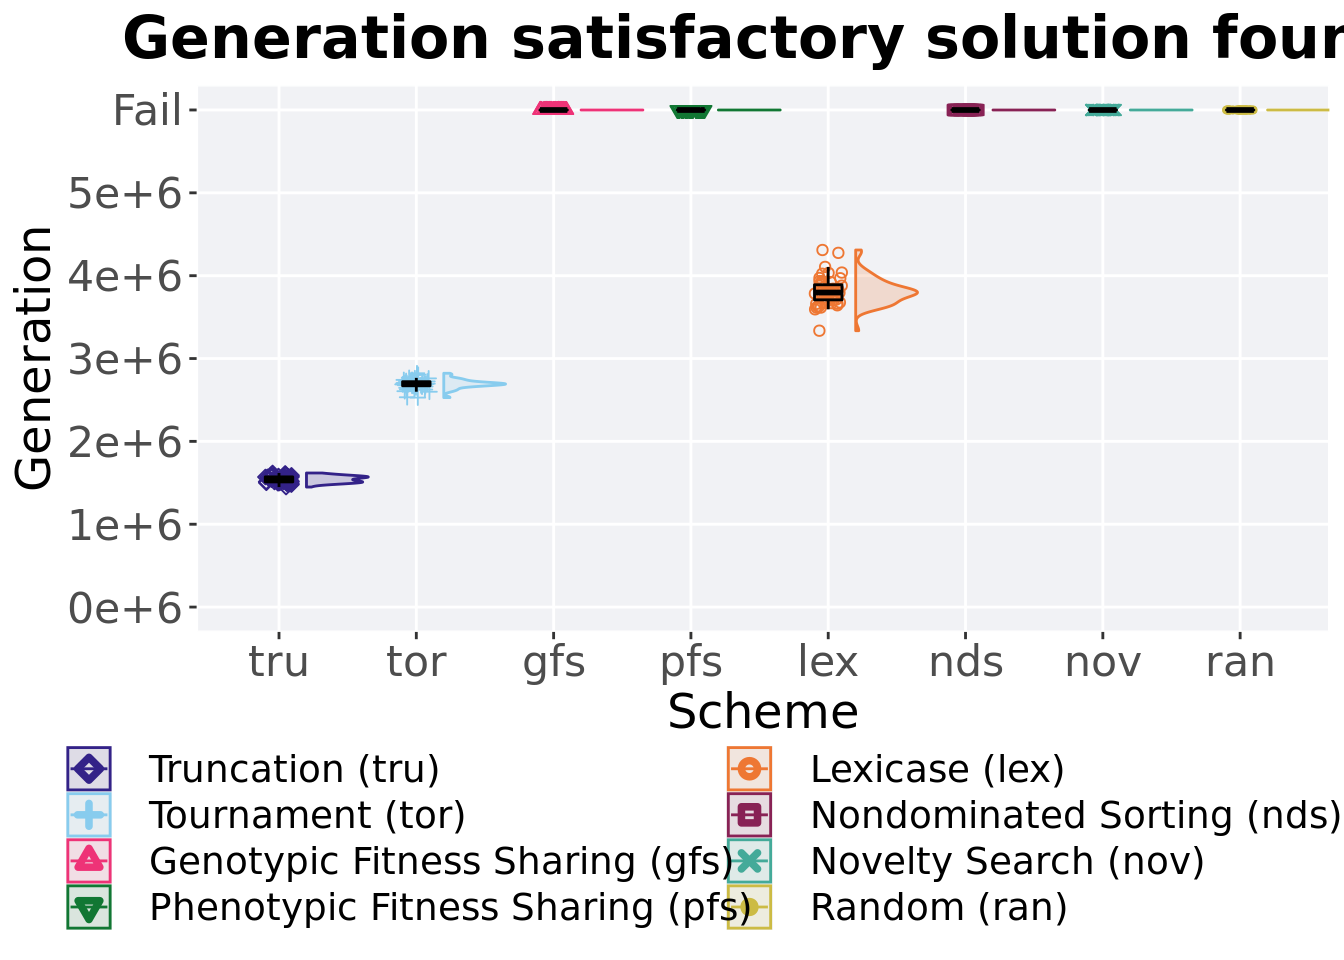
\includegraphics{demo_files/figure-latex/unnamed-chunk-21-1.pdf}

\hypertarget{stats-3}{%
\subsection{Stats}\label{stats-3}}

Summary statistics for the first generation a satisfactory solution is found throughout the 50,000 generations.

\begin{Shaded}
\begin{Highlighting}[]
\NormalTok{schemes <-}\StringTok{ }\KeywordTok{filter}\NormalTok{(schemes, acron }\OperatorTok{==}\StringTok{ 'tru'} \OperatorTok{|}\StringTok{ }\NormalTok{acron }\OperatorTok{==}\StringTok{ 'tor'} \OperatorTok{|}\StringTok{ }\NormalTok{acron }\OperatorTok{==}\StringTok{ 'lex'}\NormalTok{)}
\KeywordTok{group_by}\NormalTok{(schemes, acron) }\OperatorTok
\StringTok{  }\NormalTok{dplyr}\OperatorTok{::}\KeywordTok{summarise}\NormalTok{(}
    \DataTypeTok{count =} \KeywordTok{n}\NormalTok{(),}
    \DataTypeTok{na_cnt =} \KeywordTok{sum}\NormalTok{(}\KeywordTok{is.na}\NormalTok{(generation)),}
    \DataTypeTok{min =} \KeywordTok{min}\NormalTok{(generation, }\DataTypeTok{na.rm =} \OtherTok{TRUE}\NormalTok{),}
    \DataTypeTok{median =} \KeywordTok{median}\NormalTok{(generation, }\DataTypeTok{na.rm =} \OtherTok{TRUE}\NormalTok{),}
    \DataTypeTok{mean =} \KeywordTok{mean}\NormalTok{(generation, }\DataTypeTok{na.rm =} \OtherTok{TRUE}\NormalTok{),}
    \DataTypeTok{max =} \KeywordTok{max}\NormalTok{(generation, }\DataTypeTok{na.rm =} \OtherTok{TRUE}\NormalTok{),}
    \DataTypeTok{IQR =} \KeywordTok{IQR}\NormalTok{(generation, }\DataTypeTok{na.rm =} \OtherTok{TRUE}\NormalTok{)}
\NormalTok{  )}
\end{Highlighting}
\end{Shaded}

\begin{verbatim}
## # A tibble: 3 x 8
##   acron count na_cnt   min median   mean   max   IQR
##   <fct> <int>  <int> <dbl>  <dbl>  <dbl> <dbl> <dbl>
## 1 tru      50      0 14487 15446. 15428. 16184  609.
## 2 tor      50      0 25283 26926. 26922. 28222  496.
## 3 lex      50      0 33359 37966. 38119. 43099 1820.
\end{verbatim}

Kruskal--Wallis test provides evidence of difference amoung selection schemes the first generation a satisfactory solution is found throughout the 50,000 generations..

\begin{Shaded}
\begin{Highlighting}[]
\KeywordTok{kruskal.test}\NormalTok{(generation }\OperatorTok{~}\StringTok{ }\NormalTok{acron, }\DataTypeTok{data =}\NormalTok{ schemes)}
\end{Highlighting}
\end{Shaded}

\begin{verbatim}
## 
##  Kruskal-Wallis rank sum test
## 
## data:  generation by acron
## Kruskal-Wallis chi-squared = 132.45, df = 2, p-value < 2.2e-16
\end{verbatim}

Results for post-hoc Wilcoxon rank-sum test with a Bonferroni correction on the first generation a satisfactory solution is found throughout the 50,000 generations.

\begin{Shaded}
\begin{Highlighting}[]
\KeywordTok{pairwise.wilcox.test}\NormalTok{(}\DataTypeTok{x =}\NormalTok{ schemes}\OperatorTok{$}\NormalTok{generation, }\DataTypeTok{g =}\NormalTok{ schemes}\OperatorTok{$}\NormalTok{acron, }\DataTypeTok{p.adjust.method =} \StringTok{"bonferroni"}\NormalTok{,}
                     \DataTypeTok{paired =} \OtherTok{FALSE}\NormalTok{, }\DataTypeTok{conf.int =} \OtherTok{FALSE}\NormalTok{, }\DataTypeTok{alternative =} \StringTok{'g'}\NormalTok{)}
\end{Highlighting}
\end{Shaded}

\begin{verbatim}
## 
##  Pairwise comparisons using Wilcoxon rank sum test with continuity correction 
## 
## data:  schemes$generation and schemes$acron 
## 
##     tru    tor   
## tor <2e-16 -     
## lex <2e-16 <2e-16
## 
## P value adjustment method: bonferroni
\end{verbatim}

\hypertarget{contradictory-objectives-results}{%
\chapter{Contradictory objectives results}\label{contradictory-objectives-results}}

Here we present the results for the \textbf{satisfactory trait corverage} and \textbf{activation gene coverage} generated by each selection scheme replicate on the contradictory objectives diagnostic.
Note both of these values are gathered at the population-level.
Activation gene coverage refers to the count of unique activation genes in a given population; this gives us a range of integers between 0 and 100.
Satisfactory trait coverage refers to the count of unique satisfied traits in a given population; this gives us a range of integers between 0 and 100.

\hypertarget{analysis-dependencies-2}{%
\section{Analysis dependencies}\label{analysis-dependencies-2}}

\begin{Shaded}
\begin{Highlighting}[]
\KeywordTok{library}\NormalTok{(ggplot2)}
\KeywordTok{library}\NormalTok{(cowplot)}
\KeywordTok{library}\NormalTok{(dplyr)}
\KeywordTok{library}\NormalTok{(PupillometryR)}
\end{Highlighting}
\end{Shaded}

\hypertarget{setup-2}{%
\section{Setup}\label{setup-2}}

These analyses were conducted in the following computing environment:

\begin{Shaded}
\begin{Highlighting}[]
\KeywordTok{print}\NormalTok{(version)}
\end{Highlighting}
\end{Shaded}

\begin{verbatim}
##                _                           
## platform       x86_64-pc-linux-gnu         
## arch           x86_64                      
## os             linux-gnu                   
## system         x86_64, linux-gnu           
## status                                     
## major          4                           
## minor          2.1                         
## year           2022                        
## month          06                          
## day            23                          
## svn rev        82513                       
## language       R                           
## version.string R version 4.2.1 (2022-06-23)
## nickname       Funny-Looking Kid
\end{verbatim}

\hypertarget{satisfactory-trait-coverage}{%
\section{Satisfactory trait coverage}\label{satisfactory-trait-coverage}}

Satisfactory trait coverage analysis.

\hypertarget{coverage-over-time}{%
\subsection{Coverage over time}\label{coverage-over-time}}

Satisfactory trait coverage over time.

\begin{Shaded}
\begin{Highlighting}[]
\NormalTok{contradictory_objectives =}\StringTok{ }\KeywordTok{filter}\NormalTok{(cc_over_time, diagnostic }\OperatorTok{==}\StringTok{ 'contradictory_objectives'}\NormalTok{)}
\NormalTok{lines =}\StringTok{ }\NormalTok{contradictory_objectives }\OperatorTok
\StringTok{        }\KeywordTok{group_by}\NormalTok{(}\StringTok{`}\DataTypeTok{Selection}\CharTok{\textbackslash{}n}\DataTypeTok{Scheme}\StringTok{`}\NormalTok{, gen) }\OperatorTok
\StringTok{          }\NormalTok{dplyr}\OperatorTok{::}\KeywordTok{summarise}\NormalTok{(}
            \DataTypeTok{min =} \KeywordTok{min}\NormalTok{(pop_uni_obj),}
            \DataTypeTok{mean =} \KeywordTok{mean}\NormalTok{(pop_uni_obj),}
            \DataTypeTok{max =} \KeywordTok{max}\NormalTok{(pop_uni_obj)}
\NormalTok{          )}
\end{Highlighting}
\end{Shaded}

\begin{verbatim}
## `summarise()` has grouped output by 'Selection Scheme'. You can override using
## the `.groups` argument.
\end{verbatim}

\begin{Shaded}
\begin{Highlighting}[]
\NormalTok{points =}\StringTok{ }\KeywordTok{filter}\NormalTok{(lines, gen }\OperatorTok\StringTok{ }\DecValTok{2000} \OperatorTok{==}\StringTok{ }\DecValTok{0} \OperatorTok{&}\StringTok{ }\NormalTok{gen }\OperatorTok{!=}\StringTok{ }\DecValTok{0}\NormalTok{)}

\NormalTok{ot =}\StringTok{ }\KeywordTok{ggplot}\NormalTok{(lines, }\KeywordTok{aes}\NormalTok{(}\DataTypeTok{x=}\NormalTok{gen, }\DataTypeTok{y=}\NormalTok{mean, }\DataTypeTok{group =} \StringTok{`}\DataTypeTok{Selection}\CharTok{\textbackslash{}n}\DataTypeTok{Scheme}\StringTok{`}\NormalTok{, }\DataTypeTok{fill =}\StringTok{`}\DataTypeTok{Selection}\CharTok{\textbackslash{}n}\DataTypeTok{Scheme}\StringTok{`}\NormalTok{, }\DataTypeTok{color =} \StringTok{`}\DataTypeTok{Selection}\CharTok{\textbackslash{}n}\DataTypeTok{Scheme}\StringTok{`}\NormalTok{, }\DataTypeTok{shape =} \StringTok{`}\DataTypeTok{Selection}\CharTok{\textbackslash{}n}\DataTypeTok{Scheme}\StringTok{`}\NormalTok{)) }\OperatorTok{+}
\StringTok{  }\KeywordTok{geom_ribbon}\NormalTok{(}\KeywordTok{aes}\NormalTok{(}\DataTypeTok{ymin =}\NormalTok{ min, }\DataTypeTok{ymax =}\NormalTok{ max), }\DataTypeTok{alpha =} \FloatTok{0.1}\NormalTok{) }\OperatorTok{+}
\StringTok{  }\KeywordTok{geom_line}\NormalTok{(}\DataTypeTok{size =} \FloatTok{0.5}\NormalTok{) }\OperatorTok{+}
\StringTok{  }\KeywordTok{geom_point}\NormalTok{(}\DataTypeTok{data =}\NormalTok{ points, }\DataTypeTok{size =} \FloatTok{1.5}\NormalTok{, }\DataTypeTok{stroke =} \FloatTok{2.0}\NormalTok{, }\DataTypeTok{alpha =} \FloatTok{1.0}\NormalTok{) }\OperatorTok{+}
\StringTok{  }\KeywordTok{scale_y_continuous}\NormalTok{(}
    \DataTypeTok{name=}\StringTok{"Coverage"}\NormalTok{,}
    \DataTypeTok{limits=}\KeywordTok{c}\NormalTok{(}\OperatorTok{-}\DecValTok{1}\NormalTok{, }\DecValTok{101}\NormalTok{),}
    \DataTypeTok{breaks=}\KeywordTok{seq}\NormalTok{(}\DecValTok{0}\NormalTok{,}\DecValTok{100}\NormalTok{, }\DecValTok{20}\NormalTok{),}
    \DataTypeTok{labels=}\KeywordTok{c}\NormalTok{(}\StringTok{"0"}\NormalTok{, }\StringTok{"20"}\NormalTok{, }\StringTok{"40"}\NormalTok{, }\StringTok{"60"}\NormalTok{, }\StringTok{"80"}\NormalTok{, }\StringTok{"100"}\NormalTok{)}
\NormalTok{  ) }\OperatorTok{+}
\StringTok{  }\KeywordTok{scale_x_continuous}\NormalTok{(}
    \DataTypeTok{name=}\StringTok{"Generations"}\NormalTok{,}
    \DataTypeTok{limits=}\KeywordTok{c}\NormalTok{(}\DecValTok{0}\NormalTok{, }\DecValTok{50000}\NormalTok{),}
    \DataTypeTok{breaks=}\KeywordTok{c}\NormalTok{(}\DecValTok{0}\NormalTok{, }\DecValTok{10000}\NormalTok{, }\DecValTok{20000}\NormalTok{, }\DecValTok{30000}\NormalTok{, }\DecValTok{40000}\NormalTok{, }\DecValTok{50000}\NormalTok{),}
    \DataTypeTok{labels=}\KeywordTok{c}\NormalTok{(}\StringTok{"0e+6"}\NormalTok{, }\StringTok{"1e+6"}\NormalTok{, }\StringTok{"2e+6"}\NormalTok{, }\StringTok{"3e+6"}\NormalTok{, }\StringTok{"4e+6"}\NormalTok{, }\StringTok{"5e+6"}\NormalTok{)}

\NormalTok{  ) }\OperatorTok{+}
\StringTok{  }\KeywordTok{scale_shape_manual}\NormalTok{(}\DataTypeTok{values=}\NormalTok{SHAPE)}\OperatorTok{+}
\StringTok{  }\KeywordTok{scale_colour_manual}\NormalTok{(}\DataTypeTok{values =}\NormalTok{ cb_palette) }\OperatorTok{+}
\StringTok{  }\KeywordTok{scale_fill_manual}\NormalTok{(}\DataTypeTok{values =}\NormalTok{ cb_palette) }\OperatorTok{+}
\StringTok{  }\KeywordTok{ggtitle}\NormalTok{(}\StringTok{"Satisfactory trait coverage over time"}\NormalTok{) }\OperatorTok{+}
\StringTok{  }\NormalTok{p_theme}\OperatorTok{+}
\StringTok{    }\KeywordTok{guides}\NormalTok{(}
    \DataTypeTok{shape=}\KeywordTok{guide_legend}\NormalTok{(}\DataTypeTok{ncol=}\DecValTok{2}\NormalTok{, }\DataTypeTok{title.position =} \StringTok{"bottom"}\NormalTok{),}
    \DataTypeTok{color=}\KeywordTok{guide_legend}\NormalTok{(}\DataTypeTok{ncol=}\DecValTok{2}\NormalTok{, }\DataTypeTok{title.position =} \StringTok{"bottom"}\NormalTok{),}
    \DataTypeTok{fill=}\KeywordTok{guide_legend}\NormalTok{(}\DataTypeTok{ncol=}\DecValTok{2}\NormalTok{, }\DataTypeTok{title.position =} \StringTok{"bottom"}\NormalTok{)}
\NormalTok{  ) }\OperatorTok{+}
\StringTok{  }\KeywordTok{theme}\NormalTok{(}
    \DataTypeTok{legend.position =} \StringTok{"bottom"}\NormalTok{,}
    \DataTypeTok{legend.box=}\StringTok{"verticle"}\NormalTok{,}
    \DataTypeTok{legend.justification=}\StringTok{"center"}\NormalTok{,}
    \DataTypeTok{legend.title=}\KeywordTok{element_blank}\NormalTok{()}
\NormalTok{  )}

\NormalTok{ot}
\end{Highlighting}
\end{Shaded}

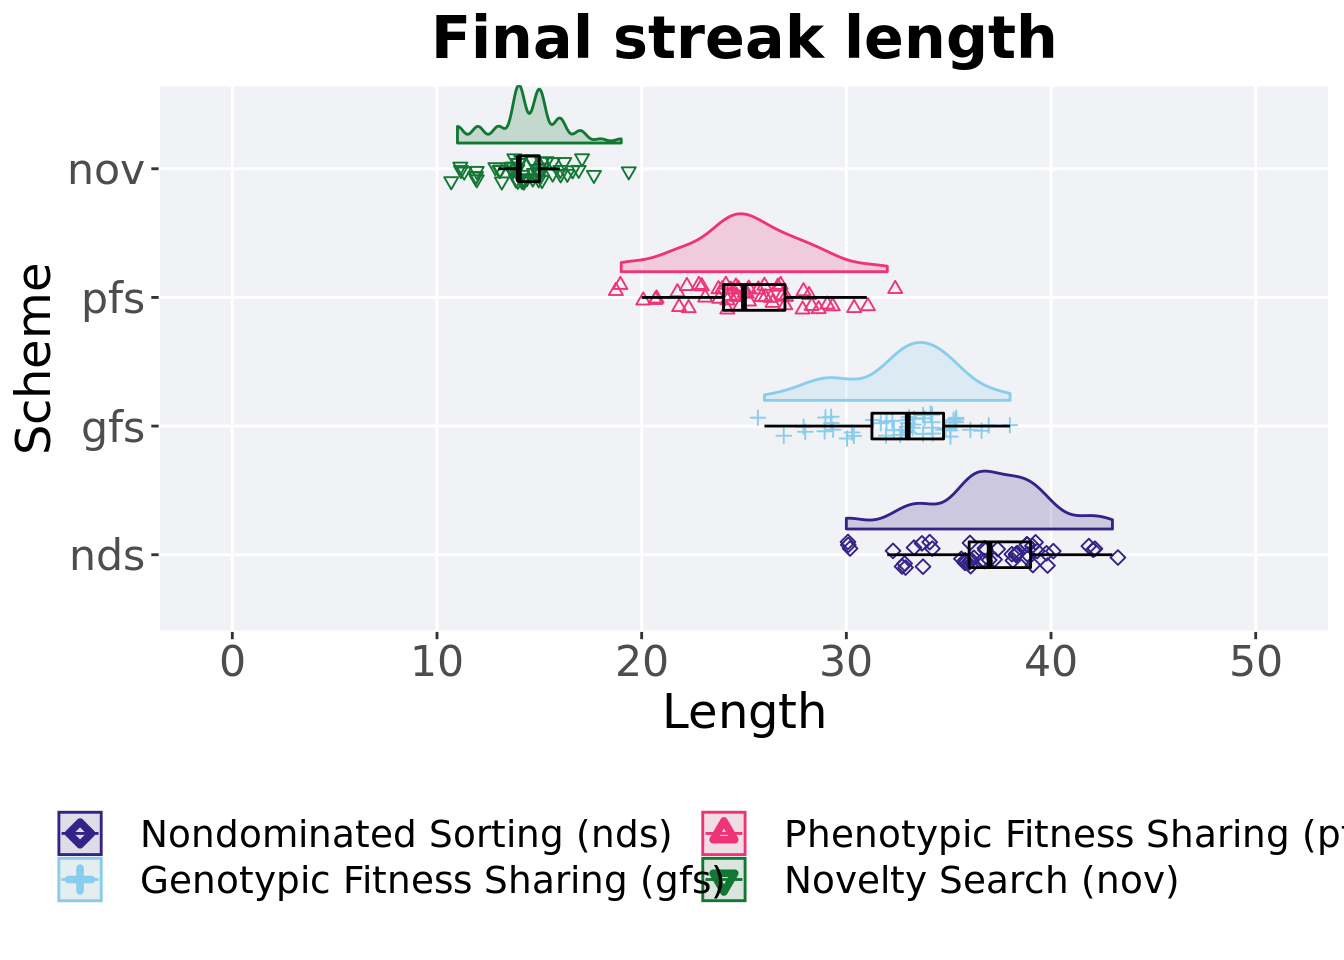
\includegraphics{demo_files/figure-latex/unnamed-chunk-27-1.pdf}

\hypertarget{best-coverage-throughout}{%
\subsection{Best coverage throughout}\label{best-coverage-throughout}}

Best satisfactory trait coverage throughout 50,000 generations.

\begin{Shaded}
\begin{Highlighting}[]
\NormalTok{best =}\StringTok{ }\KeywordTok{filter}\NormalTok{(cc_best, col }\OperatorTok{==}\StringTok{ 'pop_uni_obj'} \OperatorTok{&}\StringTok{ }\NormalTok{diagnostic }\OperatorTok{==}\StringTok{ 'contradictory_objectives'}\NormalTok{)}
\NormalTok{plot =}\StringTok{ }\KeywordTok{ggplot}\NormalTok{(best, }\KeywordTok{aes}\NormalTok{(}\DataTypeTok{x =}\NormalTok{ acron, }\DataTypeTok{y =}\NormalTok{ val, }\DataTypeTok{color =}\NormalTok{ acron, }\DataTypeTok{fill =}\NormalTok{ acron, }\DataTypeTok{shape =}\NormalTok{ acron)) }\OperatorTok{+}
\StringTok{  }\KeywordTok{geom_flat_violin}\NormalTok{(}\DataTypeTok{position =} \KeywordTok{position_nudge}\NormalTok{(}\DataTypeTok{x =} \FloatTok{.2}\NormalTok{, }\DataTypeTok{y =} \DecValTok{0}\NormalTok{), }\DataTypeTok{scale =} \StringTok{'width'}\NormalTok{, }\DataTypeTok{alpha =} \FloatTok{0.2}\NormalTok{) }\OperatorTok{+}
\StringTok{  }\KeywordTok{geom_point}\NormalTok{(}\DataTypeTok{position =} \KeywordTok{position_jitter}\NormalTok{(}\DataTypeTok{width =} \FloatTok{.1}\NormalTok{), }\DataTypeTok{size =} \FloatTok{1.5}\NormalTok{, }\DataTypeTok{alpha =} \FloatTok{1.0}\NormalTok{) }\OperatorTok{+}
\StringTok{  }\KeywordTok{geom_boxplot}\NormalTok{(}\DataTypeTok{color =} \StringTok{'black'}\NormalTok{, }\DataTypeTok{width =} \FloatTok{.2}\NormalTok{, }\DataTypeTok{outlier.shape =} \OtherTok{NA}\NormalTok{, }\DataTypeTok{alpha =} \FloatTok{0.0}\NormalTok{) }\OperatorTok{+}
\StringTok{  }\KeywordTok{scale_y_continuous}\NormalTok{(}
    \DataTypeTok{name=}\StringTok{"Coverage"}\NormalTok{,}
    \DataTypeTok{limits=}\KeywordTok{c}\NormalTok{(}\OperatorTok{-}\DecValTok{1}\NormalTok{, }\DecValTok{101}\NormalTok{),}
    \DataTypeTok{breaks=}\KeywordTok{seq}\NormalTok{(}\DecValTok{0}\NormalTok{,}\DecValTok{100}\NormalTok{, }\DecValTok{20}\NormalTok{),}
    \DataTypeTok{labels=}\KeywordTok{c}\NormalTok{(}\StringTok{"0"}\NormalTok{, }\StringTok{"20"}\NormalTok{, }\StringTok{"40"}\NormalTok{, }\StringTok{"60"}\NormalTok{, }\StringTok{"80"}\NormalTok{, }\StringTok{"100"}\NormalTok{)}
\NormalTok{  ) }\OperatorTok{+}
\StringTok{  }\KeywordTok{scale_x_discrete}\NormalTok{(}
    \DataTypeTok{name=}\StringTok{"Scheme"}
\NormalTok{  )}\OperatorTok{+}
\StringTok{  }\KeywordTok{scale_shape_manual}\NormalTok{(}\DataTypeTok{values=}\NormalTok{SHAPE)}\OperatorTok{+}
\StringTok{  }\KeywordTok{scale_colour_manual}\NormalTok{(}\DataTypeTok{values =}\NormalTok{ cb_palette) }\OperatorTok{+}
\StringTok{  }\KeywordTok{scale_fill_manual}\NormalTok{(}\DataTypeTok{values =}\NormalTok{ cb_palette) }\OperatorTok{+}
\StringTok{  }\NormalTok{p_theme}

\KeywordTok{plot_grid}\NormalTok{(}
\NormalTok{  plot }\OperatorTok{+}
\StringTok{    }\KeywordTok{ggtitle}\NormalTok{(}\StringTok{"Best satisfactory trait coverage"}\NormalTok{) }\OperatorTok{+}
\StringTok{    }\KeywordTok{theme}\NormalTok{(}\DataTypeTok{legend.position=}\StringTok{"none"}\NormalTok{),}
\NormalTok{  legend,}
  \DataTypeTok{nrow=}\DecValTok{2}\NormalTok{,}
  \DataTypeTok{rel_heights =} \KeywordTok{c}\NormalTok{(}\DecValTok{2}\NormalTok{,.}\DecValTok{55}\NormalTok{),}
  \DataTypeTok{label_size =}\NormalTok{ TSIZE}
\NormalTok{)}
\end{Highlighting}
\end{Shaded}

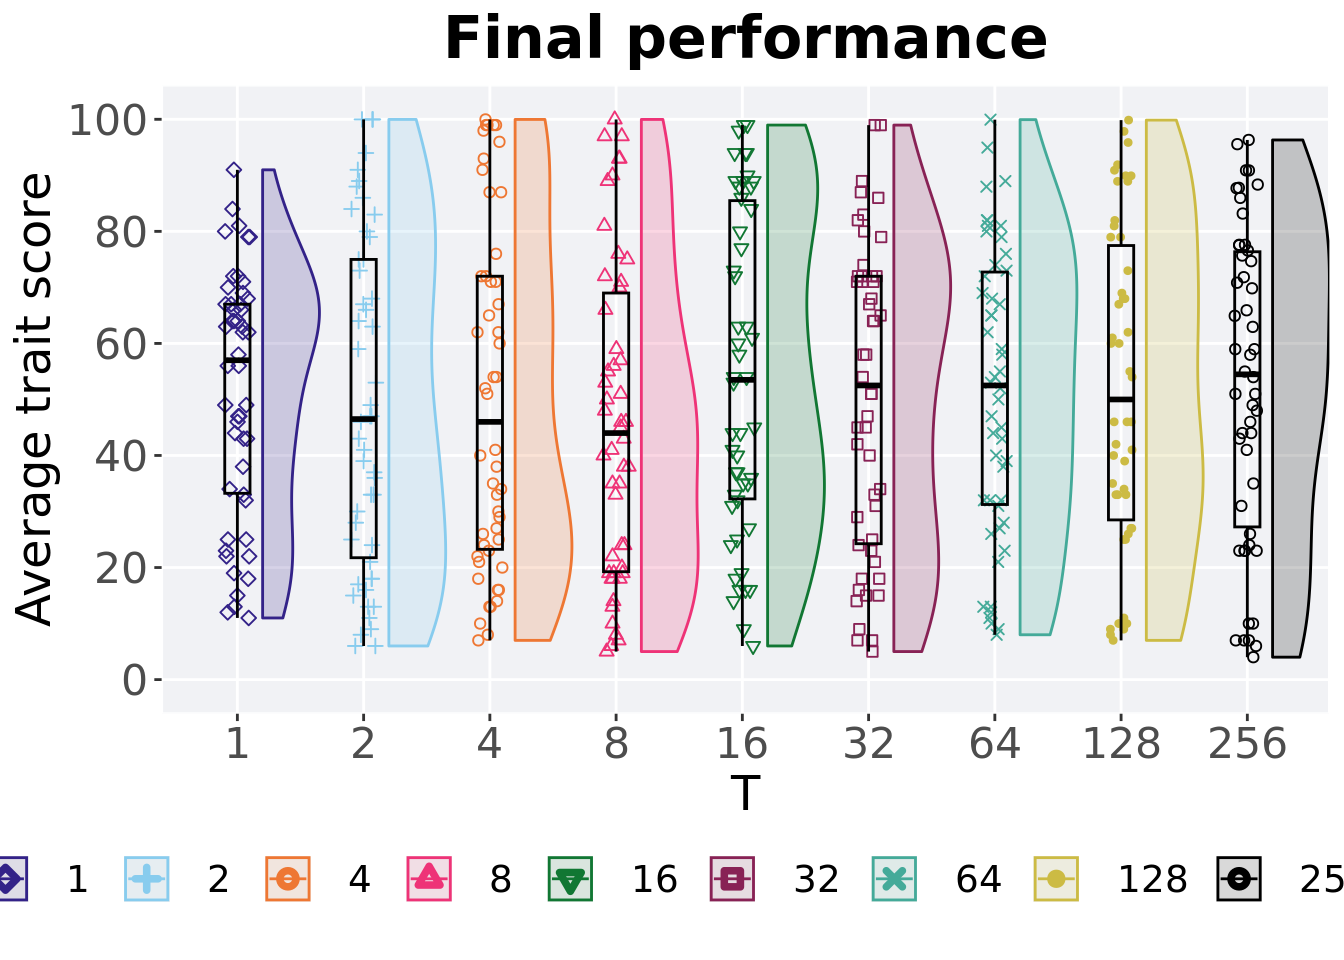
\includegraphics{demo_files/figure-latex/unnamed-chunk-29-1.pdf}

\hypertarget{stats-4}{%
\subsubsection{Stats}\label{stats-4}}

Summary statistics for the best satisfactory trait coverage throughout 50,000 generations.

\begin{Shaded}
\begin{Highlighting}[]
\NormalTok{best}\OperatorTok{$}\NormalTok{acron =}\StringTok{ }\KeywordTok{factor}\NormalTok{(best}\OperatorTok{$}\NormalTok{acron, }\DataTypeTok{levels =} \KeywordTok{c}\NormalTok{(}\StringTok{'nds'}\NormalTok{, }\StringTok{'lex'}\NormalTok{, }\StringTok{'pfs'}\NormalTok{, }\StringTok{'gfs'}\NormalTok{, }\StringTok{'tor'}\NormalTok{, }\StringTok{'tru'}\NormalTok{, }\StringTok{'nov'}\NormalTok{, }\StringTok{'ran'}\NormalTok{))}
\KeywordTok{group_by}\NormalTok{(best, acron) }\OperatorTok
\StringTok{  }\NormalTok{dplyr}\OperatorTok{::}\KeywordTok{summarise}\NormalTok{(}
    \DataTypeTok{count =} \KeywordTok{n}\NormalTok{(),}
    \DataTypeTok{na_cnt =} \KeywordTok{sum}\NormalTok{(}\KeywordTok{is.na}\NormalTok{(val)),}
    \DataTypeTok{min =} \KeywordTok{min}\NormalTok{(val, }\DataTypeTok{na.rm =} \OtherTok{TRUE}\NormalTok{),}
    \DataTypeTok{median =} \KeywordTok{median}\NormalTok{(val, }\DataTypeTok{na.rm =} \OtherTok{TRUE}\NormalTok{),}
    \DataTypeTok{mean =} \KeywordTok{mean}\NormalTok{(val, }\DataTypeTok{na.rm =} \OtherTok{TRUE}\NormalTok{),}
    \DataTypeTok{max =} \KeywordTok{max}\NormalTok{(val, }\DataTypeTok{na.rm =} \OtherTok{TRUE}\NormalTok{),}
    \DataTypeTok{IQR =} \KeywordTok{IQR}\NormalTok{(val, }\DataTypeTok{na.rm =} \OtherTok{TRUE}\NormalTok{)}
\NormalTok{  )}
\end{Highlighting}
\end{Shaded}

\begin{verbatim}
## # A tibble: 8 x 8
##   acron count na_cnt   min median  mean   max   IQR
##   <fct> <int>  <int> <dbl>  <dbl> <dbl> <dbl> <dbl>
## 1 nds      50      0    87     92 92.6    100  4.75
## 2 lex      50      0    46     48 48.0     51  2   
## 3 pfs      50      0     2      4  4.12     8  2   
## 4 gfs      50      0     1      1  1        1  0   
## 5 tor      50      0     1      1  1        1  0   
## 6 tru      50      0     1      1  1        1  0   
## 7 nov      50      0     0      0  0        0  0   
## 8 ran      50      0     0      0  0        0  0
\end{verbatim}

Kruskal--Wallis test provides evidence of difference among satisfactory trait coverage throughout 50,000 generations.

\begin{Shaded}
\begin{Highlighting}[]
\KeywordTok{kruskal.test}\NormalTok{(val }\OperatorTok{~}\StringTok{ }\NormalTok{acron,}\DataTypeTok{data =}\NormalTok{ best)}
\end{Highlighting}
\end{Shaded}

\begin{verbatim}
## 
##  Kruskal-Wallis rank sum test
## 
## data:  val by acron
## Kruskal-Wallis chi-squared = 396.62, df = 7, p-value < 2.2e-16
\end{verbatim}

Results for post-hoc Wilcoxon rank-sum test with a Bonferroni correction on satisfactory trait coverage throughout 50,000 generations.

\begin{Shaded}
\begin{Highlighting}[]
\KeywordTok{pairwise.wilcox.test}\NormalTok{(}\DataTypeTok{x =}\NormalTok{ best}\OperatorTok{$}\NormalTok{val, }\DataTypeTok{g =}\NormalTok{ best}\OperatorTok{$}\NormalTok{acron, }\DataTypeTok{p.adjust.method =} \StringTok{"bonferroni"}\NormalTok{,}
                     \DataTypeTok{paired =} \OtherTok{FALSE}\NormalTok{, }\DataTypeTok{conf.int =} \OtherTok{FALSE}\NormalTok{, }\DataTypeTok{alternative =} \StringTok{'l'}\NormalTok{)}
\end{Highlighting}
\end{Shaded}

\begin{verbatim}
## 
##  Pairwise comparisons using Wilcoxon rank sum test with continuity correction 
## 
## data:  best$val and best$acron 
## 
##     nds    lex    pfs    gfs    tor    tru    nov
## lex <2e-16 -      -      -      -      -      -  
## pfs <2e-16 <2e-16 -      -      -      -      -  
## gfs <2e-16 <2e-16 <2e-16 -      -      -      -  
## tor <2e-16 <2e-16 <2e-16 1      -      -      -  
## tru <2e-16 <2e-16 <2e-16 1      1      -      -  
## nov <2e-16 <2e-16 <2e-16 <2e-16 <2e-16 <2e-16 -  
## ran <2e-16 <2e-16 <2e-16 <2e-16 <2e-16 <2e-16 1  
## 
## P value adjustment method: bonferroni
\end{verbatim}

\hypertarget{end-of-50000-generations}{%
\subsection{End of 50,000 generations}\label{end-of-50000-generations}}

Satisfactory trait coverage in the population at the end of 50,000 generations.

\begin{Shaded}
\begin{Highlighting}[]
\NormalTok{end =}\StringTok{ }\KeywordTok{filter}\NormalTok{(cc_end, diagnostic }\OperatorTok{==}\StringTok{ 'contradictory_objectives'}\NormalTok{)}
\NormalTok{plot =}\StringTok{ }\KeywordTok{ggplot}\NormalTok{(end, }\KeywordTok{aes}\NormalTok{(}\DataTypeTok{x =}\NormalTok{ acron, }\DataTypeTok{y =}\NormalTok{ pop_uni_obj, }\DataTypeTok{color =}\NormalTok{ acron, }\DataTypeTok{fill =}\NormalTok{ acron, }\DataTypeTok{shape =}\NormalTok{ acron)) }\OperatorTok{+}
\StringTok{  }\KeywordTok{geom_flat_violin}\NormalTok{(}\DataTypeTok{position =} \KeywordTok{position_nudge}\NormalTok{(}\DataTypeTok{x =} \FloatTok{.2}\NormalTok{, }\DataTypeTok{y =} \DecValTok{0}\NormalTok{), }\DataTypeTok{scale =} \StringTok{'width'}\NormalTok{, }\DataTypeTok{alpha =} \FloatTok{0.2}\NormalTok{) }\OperatorTok{+}
\StringTok{  }\KeywordTok{geom_point}\NormalTok{(}\DataTypeTok{position =} \KeywordTok{position_jitter}\NormalTok{(}\DataTypeTok{width =} \FloatTok{.1}\NormalTok{), }\DataTypeTok{size =} \FloatTok{1.5}\NormalTok{, }\DataTypeTok{alpha =} \FloatTok{1.0}\NormalTok{) }\OperatorTok{+}
\StringTok{  }\KeywordTok{geom_boxplot}\NormalTok{(}\DataTypeTok{color =} \StringTok{'black'}\NormalTok{, }\DataTypeTok{width =} \FloatTok{.2}\NormalTok{, }\DataTypeTok{outlier.shape =} \OtherTok{NA}\NormalTok{, }\DataTypeTok{alpha =} \FloatTok{0.0}\NormalTok{) }\OperatorTok{+}
\StringTok{  }\KeywordTok{scale_y_continuous}\NormalTok{(}
    \DataTypeTok{name=}\StringTok{"Coverage"}\NormalTok{,}
    \DataTypeTok{limits=}\KeywordTok{c}\NormalTok{(}\OperatorTok{-}\DecValTok{1}\NormalTok{, }\DecValTok{101}\NormalTok{),}
    \DataTypeTok{breaks=}\KeywordTok{seq}\NormalTok{(}\DecValTok{0}\NormalTok{,}\DecValTok{100}\NormalTok{, }\DecValTok{20}\NormalTok{),}
    \DataTypeTok{labels=}\KeywordTok{c}\NormalTok{(}\StringTok{"0"}\NormalTok{, }\StringTok{"20"}\NormalTok{, }\StringTok{"40"}\NormalTok{, }\StringTok{"60"}\NormalTok{, }\StringTok{"80"}\NormalTok{, }\StringTok{"100"}\NormalTok{)}
\NormalTok{  ) }\OperatorTok{+}
\StringTok{  }\KeywordTok{scale_x_discrete}\NormalTok{(}
    \DataTypeTok{name=}\StringTok{"Scheme"}
\NormalTok{  )}\OperatorTok{+}
\StringTok{  }\KeywordTok{scale_shape_manual}\NormalTok{(}\DataTypeTok{values=}\NormalTok{SHAPE)}\OperatorTok{+}
\StringTok{  }\KeywordTok{scale_colour_manual}\NormalTok{(}\DataTypeTok{values =}\NormalTok{ cb_palette) }\OperatorTok{+}
\StringTok{  }\KeywordTok{scale_fill_manual}\NormalTok{(}\DataTypeTok{values =}\NormalTok{ cb_palette) }\OperatorTok{+}
\StringTok{  }\NormalTok{p_theme}

\KeywordTok{plot_grid}\NormalTok{(}
\NormalTok{  plot }\OperatorTok{+}
\StringTok{    }\KeywordTok{ggtitle}\NormalTok{(}\StringTok{"Final satisfactory trait coverage"}\NormalTok{) }\OperatorTok{+}
\StringTok{    }\KeywordTok{theme}\NormalTok{(}\DataTypeTok{legend.position=}\StringTok{"none"}\NormalTok{),}
\NormalTok{  legend,}
  \DataTypeTok{nrow=}\DecValTok{2}\NormalTok{,}
  \DataTypeTok{rel_heights =} \KeywordTok{c}\NormalTok{(}\DecValTok{2}\NormalTok{,.}\DecValTok{55}\NormalTok{),}
  \DataTypeTok{label_size =}\NormalTok{ TSIZE}
\NormalTok{)}
\end{Highlighting}
\end{Shaded}

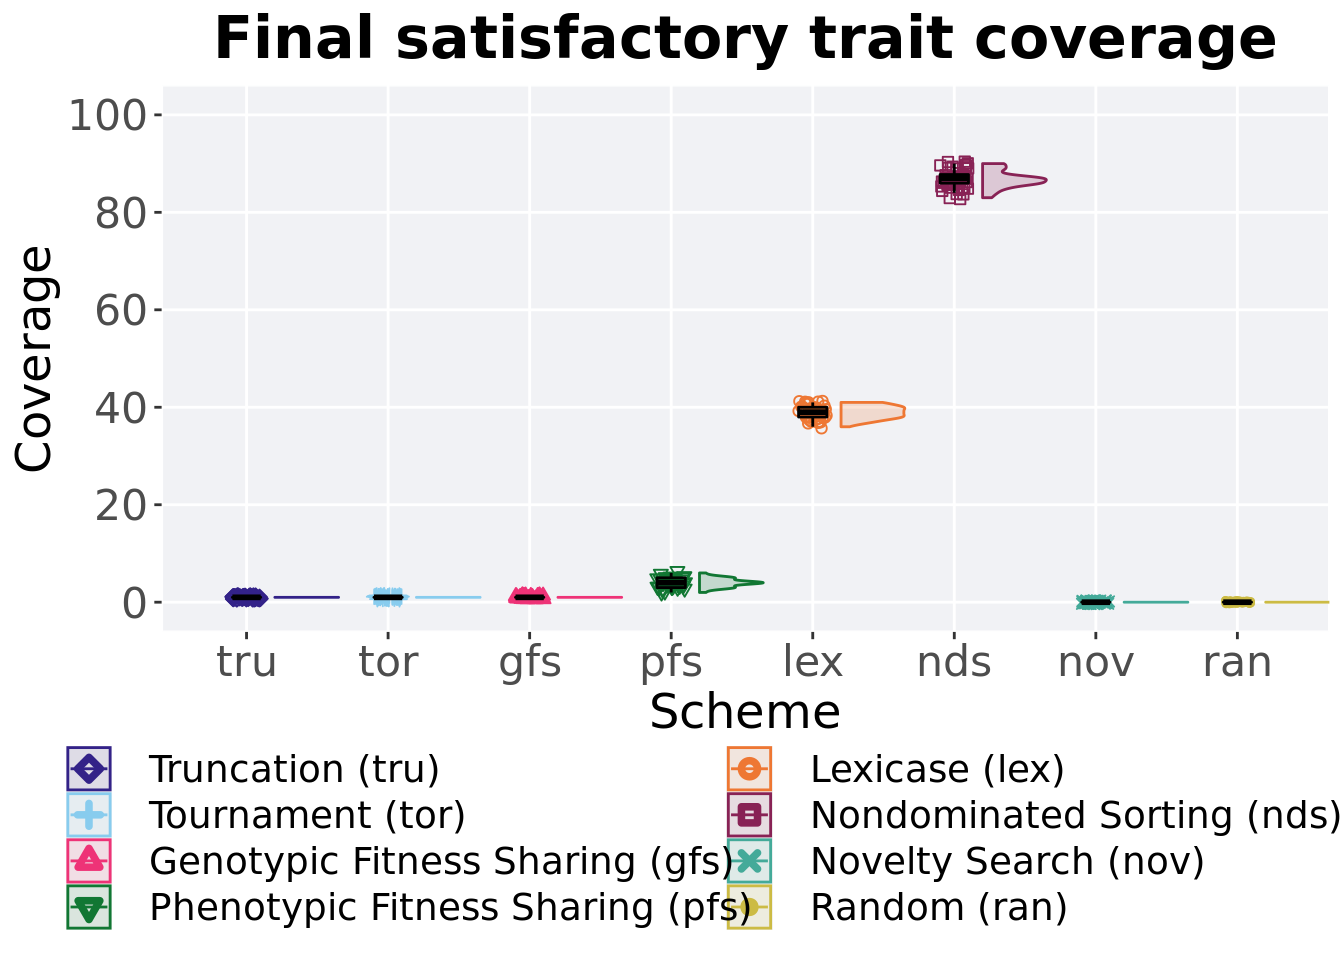
\includegraphics{demo_files/figure-latex/unnamed-chunk-33-1.pdf}

\hypertarget{stats-5}{%
\subsubsection{Stats}\label{stats-5}}

Summary statistics for satisfactory trait coverage in the population at the end of 50,000 generations.

\begin{Shaded}
\begin{Highlighting}[]
\NormalTok{end}\OperatorTok{$}\NormalTok{acron =}\StringTok{ }\KeywordTok{factor}\NormalTok{(end}\OperatorTok{$}\NormalTok{acron, }\DataTypeTok{levels =} \KeywordTok{c}\NormalTok{(}\StringTok{'nds'}\NormalTok{, }\StringTok{'lex'}\NormalTok{, }\StringTok{'pfs'}\NormalTok{, }\StringTok{'gfs'}\NormalTok{, }\StringTok{'tor'}\NormalTok{, }\StringTok{'tru'}\NormalTok{, }\StringTok{'nov'}\NormalTok{, }\StringTok{'ran'}\NormalTok{))}
\KeywordTok{group_by}\NormalTok{(end, acron) }\OperatorTok
\StringTok{  }\NormalTok{dplyr}\OperatorTok{::}\KeywordTok{summarise}\NormalTok{(}
    \DataTypeTok{count =} \KeywordTok{n}\NormalTok{(),}
    \DataTypeTok{na_cnt =} \KeywordTok{sum}\NormalTok{(}\KeywordTok{is.na}\NormalTok{(pop_uni_obj)),}
    \DataTypeTok{min =} \KeywordTok{min}\NormalTok{(pop_uni_obj, }\DataTypeTok{na.rm =} \OtherTok{TRUE}\NormalTok{),}
    \DataTypeTok{median =} \KeywordTok{median}\NormalTok{(pop_uni_obj, }\DataTypeTok{na.rm =} \OtherTok{TRUE}\NormalTok{),}
    \DataTypeTok{mean =} \KeywordTok{mean}\NormalTok{(pop_uni_obj, }\DataTypeTok{na.rm =} \OtherTok{TRUE}\NormalTok{),}
    \DataTypeTok{max =} \KeywordTok{max}\NormalTok{(pop_uni_obj, }\DataTypeTok{na.rm =} \OtherTok{TRUE}\NormalTok{),}
    \DataTypeTok{IQR =} \KeywordTok{IQR}\NormalTok{(pop_uni_obj, }\DataTypeTok{na.rm =} \OtherTok{TRUE}\NormalTok{)}
\NormalTok{  )}
\end{Highlighting}
\end{Shaded}

\begin{verbatim}
## # A tibble: 8 x 8
##   acron count na_cnt   min median  mean   max   IQR
##   <fct> <int>  <int> <int>  <dbl> <dbl> <int> <dbl>
## 1 nds      50      0    83     87  86.8    90  1.75
## 2 lex      50      0    36     39  39.0    41  2   
## 3 pfs      50      0     2      4   4       6  2   
## 4 gfs      50      0     1      1   1       1  0   
## 5 tor      50      0     1      1   1       1  0   
## 6 tru      50      0     1      1   1       1  0   
## 7 nov      50      0     0      0   0       0  0   
## 8 ran      50      0     0      0   0       0  0
\end{verbatim}

Kruskal--Wallis test provides evidence of difference among satisfactory trait coverage in the population at the end of 50,000 generations.

\begin{Shaded}
\begin{Highlighting}[]
\KeywordTok{kruskal.test}\NormalTok{(pop_uni_obj }\OperatorTok{~}\StringTok{ }\NormalTok{acron,}\DataTypeTok{data =}\NormalTok{ end)}
\end{Highlighting}
\end{Shaded}

\begin{verbatim}
## 
##  Kruskal-Wallis rank sum test
## 
## data:  pop_uni_obj by acron
## Kruskal-Wallis chi-squared = 396.66, df = 7, p-value < 2.2e-16
\end{verbatim}

Results for post-hoc Wilcoxon rank-sum test with a Bonferroni correction on satisfactory trait coverage in the population at the end of 50,000 generations.

\begin{Shaded}
\begin{Highlighting}[]
\KeywordTok{pairwise.wilcox.test}\NormalTok{(}\DataTypeTok{x =}\NormalTok{ end}\OperatorTok{$}\NormalTok{pop_uni_obj, }\DataTypeTok{g =}\NormalTok{ end}\OperatorTok{$}\NormalTok{acron, }\DataTypeTok{p.adjust.method =} \StringTok{"bonferroni"}\NormalTok{,}
                     \DataTypeTok{paired =} \OtherTok{FALSE}\NormalTok{, }\DataTypeTok{conf.int =} \OtherTok{FALSE}\NormalTok{, }\DataTypeTok{alternative =} \StringTok{'l'}\NormalTok{)}
\end{Highlighting}
\end{Shaded}

\begin{verbatim}
## 
##  Pairwise comparisons using Wilcoxon rank sum test with continuity correction 
## 
## data:  end$pop_uni_obj and end$acron 
## 
##     nds    lex    pfs    gfs    tor    tru    nov
## lex <2e-16 -      -      -      -      -      -  
## pfs <2e-16 <2e-16 -      -      -      -      -  
## gfs <2e-16 <2e-16 <2e-16 -      -      -      -  
## tor <2e-16 <2e-16 <2e-16 1      -      -      -  
## tru <2e-16 <2e-16 <2e-16 1      1      -      -  
## nov <2e-16 <2e-16 <2e-16 <2e-16 <2e-16 <2e-16 -  
## ran <2e-16 <2e-16 <2e-16 <2e-16 <2e-16 <2e-16 1  
## 
## P value adjustment method: bonferroni
\end{verbatim}

\hypertarget{activation-gene-coverage}{%
\section{Activation gene coverage}\label{activation-gene-coverage}}

Activation gene coverage analysis.

\hypertarget{over-time-coverage}{%
\subsection{Over time coverage}\label{over-time-coverage}}

Activation gene coverage over time.

\begin{Shaded}
\begin{Highlighting}[]
\NormalTok{contradictory_objectives =}\StringTok{ }\KeywordTok{filter}\NormalTok{(cc_over_time, diagnostic }\OperatorTok{==}\StringTok{ 'contradictory_objectives'}\NormalTok{)}
\NormalTok{contradictory_objectives}\OperatorTok{$}\NormalTok{uni_str_pos =}\StringTok{ }\NormalTok{contradictory_objectives}\OperatorTok{$}\NormalTok{uni_str_pos }\OperatorTok{+}\StringTok{ }\NormalTok{contradictory_objectives}\OperatorTok{$}\NormalTok{arc_acti_gene }\OperatorTok{-}\StringTok{ }\NormalTok{contradictory_objectives}\OperatorTok{$}\NormalTok{overlap}
\NormalTok{lines =}\StringTok{ }\NormalTok{contradictory_objectives }\OperatorTok
\StringTok{        }\KeywordTok{group_by}\NormalTok{(}\StringTok{`}\DataTypeTok{Selection}\CharTok{\textbackslash{}n}\DataTypeTok{Scheme}\StringTok{`}\NormalTok{, gen) }\OperatorTok
\StringTok{          }\NormalTok{dplyr}\OperatorTok{::}\KeywordTok{summarise}\NormalTok{(}
            \DataTypeTok{min =} \KeywordTok{min}\NormalTok{(uni_str_pos),}
            \DataTypeTok{mean =} \KeywordTok{mean}\NormalTok{(uni_str_pos),}
            \DataTypeTok{max =} \KeywordTok{max}\NormalTok{(uni_str_pos)}
\NormalTok{          )}
\end{Highlighting}
\end{Shaded}

\begin{verbatim}
## `summarise()` has grouped output by 'Selection Scheme'. You can override using
## the `.groups` argument.
\end{verbatim}

\begin{Shaded}
\begin{Highlighting}[]
\NormalTok{points =}\StringTok{ }\KeywordTok{filter}\NormalTok{(lines, gen }\OperatorTok\StringTok{ }\DecValTok{2000} \OperatorTok{==}\StringTok{ }\DecValTok{0} \OperatorTok{&}\StringTok{ }\NormalTok{gen }\OperatorTok{!=}\StringTok{ }\DecValTok{0}\NormalTok{)}

\NormalTok{ot =}\StringTok{ }\KeywordTok{ggplot}\NormalTok{(lines, }\KeywordTok{aes}\NormalTok{(}\DataTypeTok{x=}\NormalTok{gen, }\DataTypeTok{y=}\NormalTok{mean, }\DataTypeTok{group =} \StringTok{`}\DataTypeTok{Selection}\CharTok{\textbackslash{}n}\DataTypeTok{Scheme}\StringTok{`}\NormalTok{, }\DataTypeTok{fill =}\StringTok{`}\DataTypeTok{Selection}\CharTok{\textbackslash{}n}\DataTypeTok{Scheme}\StringTok{`}\NormalTok{, }\DataTypeTok{color =} \StringTok{`}\DataTypeTok{Selection}\CharTok{\textbackslash{}n}\DataTypeTok{Scheme}\StringTok{`}\NormalTok{, }\DataTypeTok{shape =} \StringTok{`}\DataTypeTok{Selection}\CharTok{\textbackslash{}n}\DataTypeTok{Scheme}\StringTok{`}\NormalTok{)) }\OperatorTok{+}
\StringTok{  }\KeywordTok{geom_ribbon}\NormalTok{(}\KeywordTok{aes}\NormalTok{(}\DataTypeTok{ymin =}\NormalTok{ min, }\DataTypeTok{ymax =}\NormalTok{ max), }\DataTypeTok{alpha =} \FloatTok{0.1}\NormalTok{) }\OperatorTok{+}
\StringTok{  }\KeywordTok{geom_line}\NormalTok{(}\DataTypeTok{size =} \FloatTok{0.5}\NormalTok{) }\OperatorTok{+}
\StringTok{  }\KeywordTok{geom_point}\NormalTok{(}\DataTypeTok{data =}\NormalTok{ points, }\DataTypeTok{size =} \FloatTok{1.5}\NormalTok{, }\DataTypeTok{stroke =} \FloatTok{2.0}\NormalTok{, }\DataTypeTok{alpha =} \FloatTok{1.0}\NormalTok{) }\OperatorTok{+}
\StringTok{  }\KeywordTok{scale_y_continuous}\NormalTok{(}
    \DataTypeTok{name=}\StringTok{"Coverage"}\NormalTok{,}
    \DataTypeTok{limits=}\KeywordTok{c}\NormalTok{(}\OperatorTok{-}\DecValTok{1}\NormalTok{, }\DecValTok{101}\NormalTok{),}
    \DataTypeTok{breaks=}\KeywordTok{seq}\NormalTok{(}\DecValTok{0}\NormalTok{,}\DecValTok{100}\NormalTok{, }\DecValTok{20}\NormalTok{),}
    \DataTypeTok{labels=}\KeywordTok{c}\NormalTok{(}\StringTok{"0"}\NormalTok{, }\StringTok{"20"}\NormalTok{, }\StringTok{"40"}\NormalTok{, }\StringTok{"60"}\NormalTok{, }\StringTok{"80"}\NormalTok{, }\StringTok{"100"}\NormalTok{)}
\NormalTok{  ) }\OperatorTok{+}
\StringTok{  }\KeywordTok{scale_x_continuous}\NormalTok{(}
    \DataTypeTok{name=}\StringTok{"Generations"}\NormalTok{,}
    \DataTypeTok{limits=}\KeywordTok{c}\NormalTok{(}\DecValTok{0}\NormalTok{, }\DecValTok{50000}\NormalTok{),}
    \DataTypeTok{breaks=}\KeywordTok{c}\NormalTok{(}\DecValTok{0}\NormalTok{, }\DecValTok{10000}\NormalTok{, }\DecValTok{20000}\NormalTok{, }\DecValTok{30000}\NormalTok{, }\DecValTok{40000}\NormalTok{, }\DecValTok{50000}\NormalTok{),}
    \DataTypeTok{labels=}\KeywordTok{c}\NormalTok{(}\StringTok{"0e+6"}\NormalTok{, }\StringTok{"1e+6"}\NormalTok{, }\StringTok{"2e+6"}\NormalTok{, }\StringTok{"3e+6"}\NormalTok{, }\StringTok{"4e+6"}\NormalTok{, }\StringTok{"5e+6"}\NormalTok{)}

\NormalTok{  ) }\OperatorTok{+}
\StringTok{  }\KeywordTok{scale_shape_manual}\NormalTok{(}\DataTypeTok{values=}\NormalTok{SHAPE)}\OperatorTok{+}
\StringTok{  }\KeywordTok{scale_colour_manual}\NormalTok{(}\DataTypeTok{values =}\NormalTok{ cb_palette) }\OperatorTok{+}
\StringTok{  }\KeywordTok{scale_fill_manual}\NormalTok{(}\DataTypeTok{values =}\NormalTok{ cb_palette) }\OperatorTok{+}
\StringTok{  }\KeywordTok{ggtitle}\NormalTok{(}\StringTok{"Activation gene coverage over time"}\NormalTok{) }\OperatorTok{+}
\StringTok{  }\NormalTok{p_theme}\OperatorTok{+}
\StringTok{    }\KeywordTok{guides}\NormalTok{(}
    \DataTypeTok{shape=}\KeywordTok{guide_legend}\NormalTok{(}\DataTypeTok{ncol=}\DecValTok{2}\NormalTok{, }\DataTypeTok{title.position =} \StringTok{"bottom"}\NormalTok{),}
    \DataTypeTok{color=}\KeywordTok{guide_legend}\NormalTok{(}\DataTypeTok{ncol=}\DecValTok{2}\NormalTok{, }\DataTypeTok{title.position =} \StringTok{"bottom"}\NormalTok{),}
    \DataTypeTok{fill=}\KeywordTok{guide_legend}\NormalTok{(}\DataTypeTok{ncol=}\DecValTok{2}\NormalTok{, }\DataTypeTok{title.position =} \StringTok{"bottom"}\NormalTok{)}
\NormalTok{  ) }\OperatorTok{+}
\StringTok{  }\KeywordTok{theme}\NormalTok{(}
    \DataTypeTok{legend.position =} \StringTok{"bottom"}\NormalTok{,}
    \DataTypeTok{legend.box=}\StringTok{"verticle"}\NormalTok{,}
    \DataTypeTok{legend.justification=}\StringTok{"center"}\NormalTok{,}
    \DataTypeTok{legend.title=}\KeywordTok{element_blank}\NormalTok{()}
\NormalTok{  )}

\NormalTok{ot}
\end{Highlighting}
\end{Shaded}

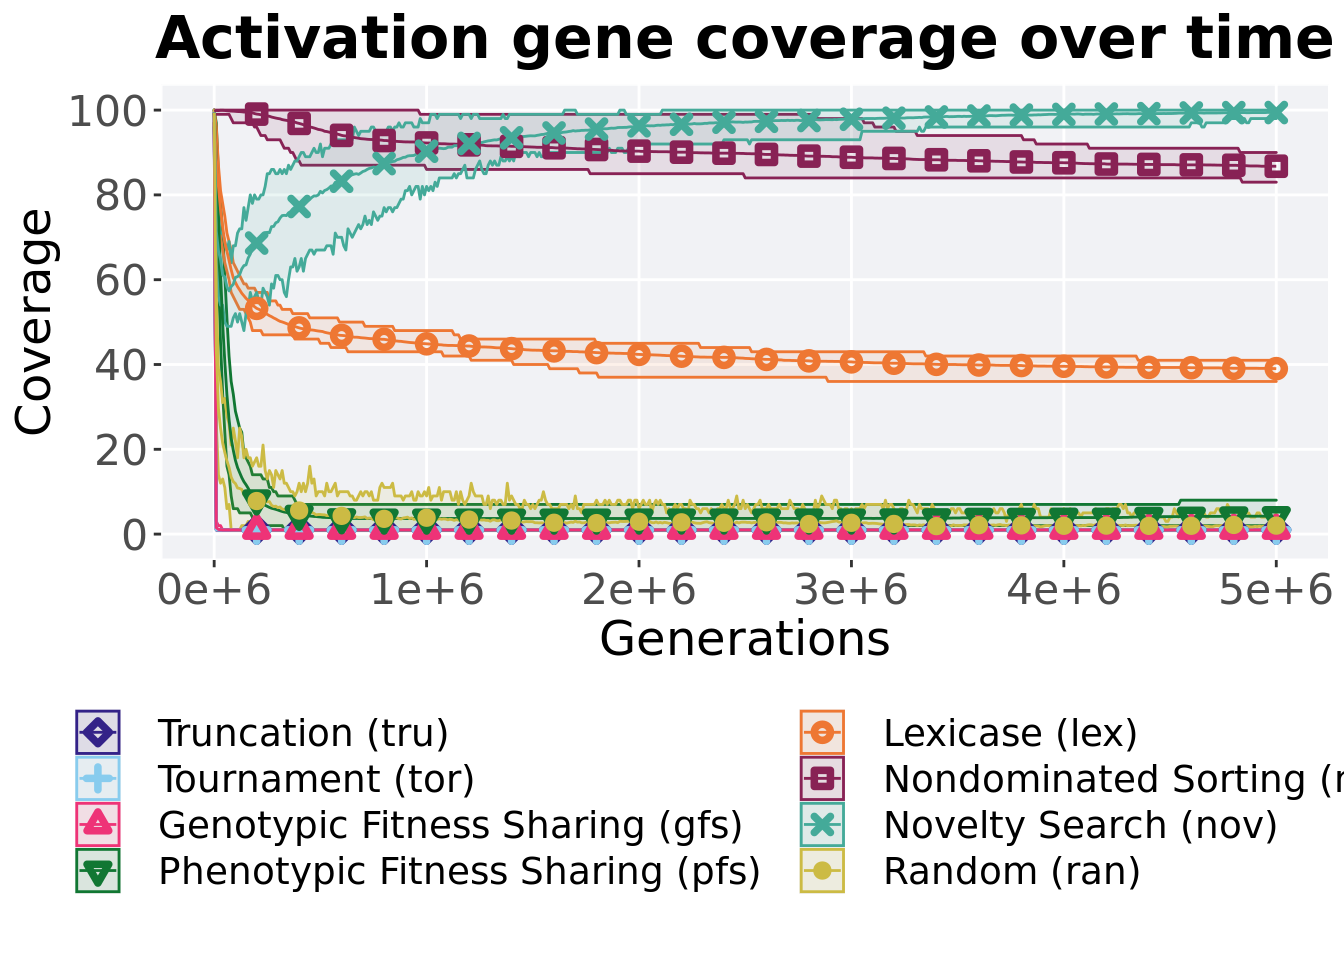
\includegraphics{demo_files/figure-latex/unnamed-chunk-37-1.pdf}

\hypertarget{end-of-50000-generations-1}{%
\subsection{End of 50,000 generations}\label{end-of-50000-generations-1}}

Activation gene coverage in the population at the end of 50,000 generations.

\begin{Shaded}
\begin{Highlighting}[]
\NormalTok{end =}\StringTok{ }\KeywordTok{filter}\NormalTok{(cc_end, diagnostic }\OperatorTok{==}\StringTok{ 'contradictory_objectives'}\NormalTok{)}
\NormalTok{end}\OperatorTok{$}\NormalTok{uni_str_pos =}\StringTok{ }\NormalTok{end}\OperatorTok{$}\NormalTok{uni_str_pos }\OperatorTok{+}\StringTok{ }\NormalTok{end}\OperatorTok{$}\NormalTok{arc_acti_gene }\OperatorTok{-}\StringTok{ }\NormalTok{end}\OperatorTok{$}\NormalTok{overlap}
\NormalTok{best =}\StringTok{ }\KeywordTok{ggplot}\NormalTok{(end, }\KeywordTok{aes}\NormalTok{(}\DataTypeTok{x =}\NormalTok{ acron, }\DataTypeTok{y =}\NormalTok{ uni_str_pos, }\DataTypeTok{color =}\NormalTok{ acron, }\DataTypeTok{fill =}\NormalTok{ acron, }\DataTypeTok{shape =}\NormalTok{ acron)) }\OperatorTok{+}
\StringTok{  }\KeywordTok{geom_flat_violin}\NormalTok{(}\DataTypeTok{position =} \KeywordTok{position_nudge}\NormalTok{(}\DataTypeTok{x =} \FloatTok{.2}\NormalTok{, }\DataTypeTok{y =} \DecValTok{0}\NormalTok{), }\DataTypeTok{scale =} \StringTok{'width'}\NormalTok{, }\DataTypeTok{alpha =} \FloatTok{0.2}\NormalTok{) }\OperatorTok{+}
\StringTok{  }\KeywordTok{geom_point}\NormalTok{(}\DataTypeTok{position =} \KeywordTok{position_jitter}\NormalTok{(}\DataTypeTok{width =} \FloatTok{.1}\NormalTok{), }\DataTypeTok{size =} \FloatTok{1.5}\NormalTok{, }\DataTypeTok{alpha =} \FloatTok{1.0}\NormalTok{) }\OperatorTok{+}
\StringTok{  }\KeywordTok{geom_boxplot}\NormalTok{(}\DataTypeTok{color =} \StringTok{'black'}\NormalTok{, }\DataTypeTok{width =} \FloatTok{.2}\NormalTok{, }\DataTypeTok{outlier.shape =} \OtherTok{NA}\NormalTok{, }\DataTypeTok{alpha =} \FloatTok{0.0}\NormalTok{) }\OperatorTok{+}
\StringTok{  }\KeywordTok{scale_y_continuous}\NormalTok{(}
    \DataTypeTok{name=}\StringTok{"Coverage"}\NormalTok{,}
    \DataTypeTok{limits=}\KeywordTok{c}\NormalTok{(}\OperatorTok{-}\DecValTok{1}\NormalTok{, }\DecValTok{101}\NormalTok{),}
    \DataTypeTok{breaks=}\KeywordTok{seq}\NormalTok{(}\DecValTok{0}\NormalTok{,}\DecValTok{100}\NormalTok{, }\DecValTok{20}\NormalTok{),}
    \DataTypeTok{labels=}\KeywordTok{c}\NormalTok{(}\StringTok{"0"}\NormalTok{, }\StringTok{"20"}\NormalTok{, }\StringTok{"40"}\NormalTok{, }\StringTok{"60"}\NormalTok{, }\StringTok{"80"}\NormalTok{, }\StringTok{"100"}\NormalTok{)}
\NormalTok{  ) }\OperatorTok{+}
\StringTok{  }\KeywordTok{scale_x_discrete}\NormalTok{(}
    \DataTypeTok{name=}\StringTok{"Scheme"}
\NormalTok{  )}\OperatorTok{+}
\StringTok{  }\KeywordTok{scale_shape_manual}\NormalTok{(}\DataTypeTok{values=}\NormalTok{SHAPE)}\OperatorTok{+}
\StringTok{  }\KeywordTok{scale_colour_manual}\NormalTok{(}\DataTypeTok{values =}\NormalTok{ cb_palette) }\OperatorTok{+}
\StringTok{  }\KeywordTok{scale_fill_manual}\NormalTok{(}\DataTypeTok{values =}\NormalTok{ cb_palette) }\OperatorTok{+}
\StringTok{  }\NormalTok{p_theme}

\KeywordTok{plot_grid}\NormalTok{(}
\NormalTok{  best }\OperatorTok{+}
\StringTok{    }\KeywordTok{ggtitle}\NormalTok{(}\StringTok{"Final activation gene coverage"}\NormalTok{) }\OperatorTok{+}
\StringTok{    }\KeywordTok{theme}\NormalTok{(}\DataTypeTok{legend.position=}\StringTok{"none"}\NormalTok{),}
\NormalTok{  legend,}
  \DataTypeTok{nrow=}\DecValTok{2}\NormalTok{,}
  \DataTypeTok{rel_heights =} \KeywordTok{c}\NormalTok{(}\DecValTok{2}\NormalTok{,.}\DecValTok{55}\NormalTok{),}
  \DataTypeTok{label_size =}\NormalTok{ TSIZE}
\NormalTok{)}
\end{Highlighting}
\end{Shaded}

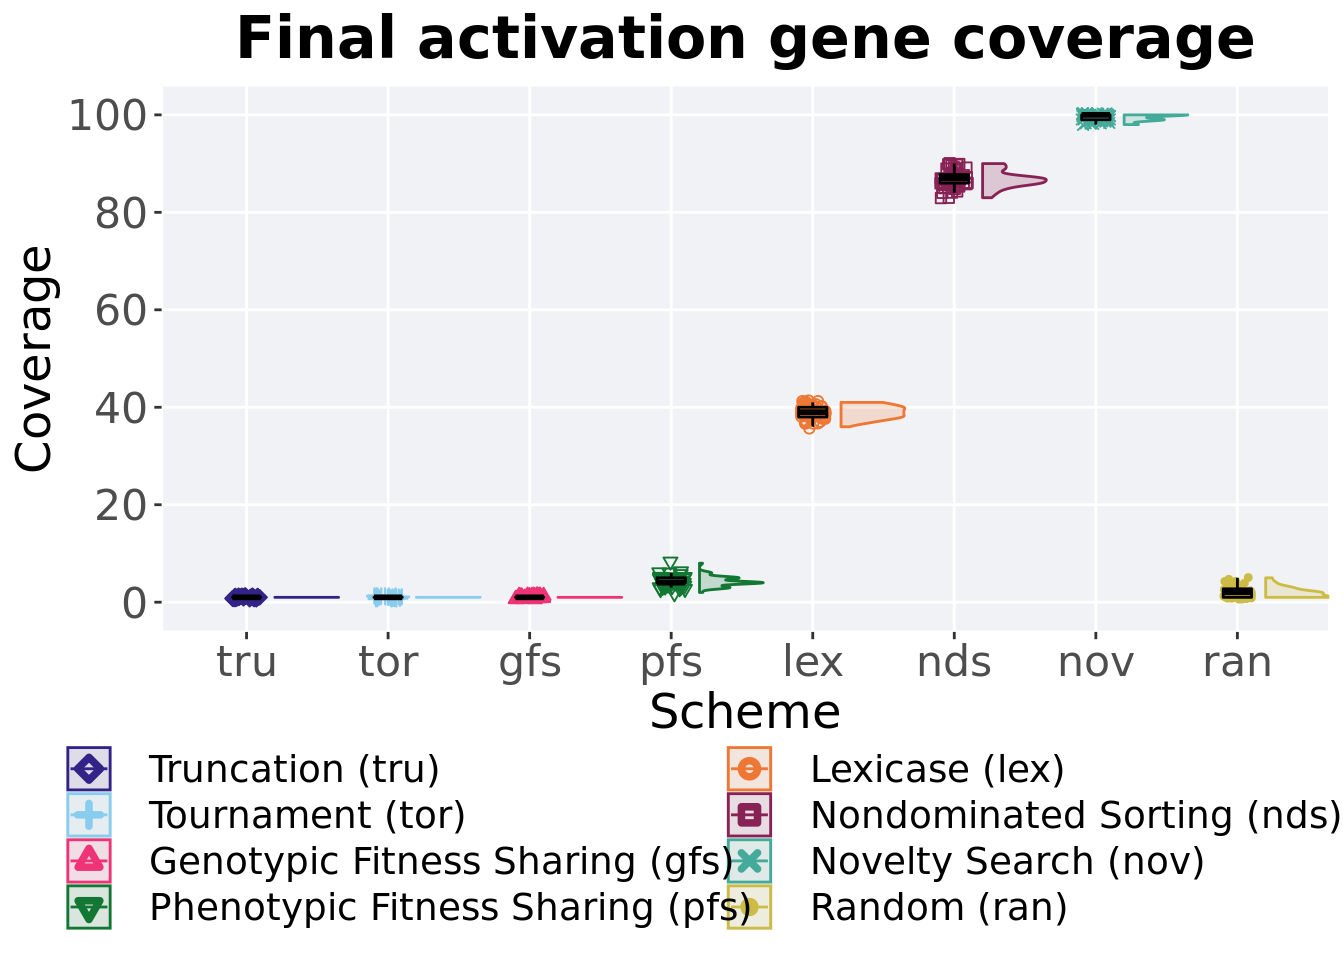
\includegraphics{demo_files/figure-latex/unnamed-chunk-38-1.pdf}

\hypertarget{stats-6}{%
\subsubsection{Stats}\label{stats-6}}

Summary statistics for activation gene coverage in the population at the end of 50,000 generations.

\begin{Shaded}
\begin{Highlighting}[]
\NormalTok{end}\OperatorTok{$}\NormalTok{acron =}\StringTok{ }\KeywordTok{factor}\NormalTok{(end}\OperatorTok{$}\NormalTok{acron, }\DataTypeTok{levels =} \KeywordTok{c}\NormalTok{(}\StringTok{'nds'}\NormalTok{, }\StringTok{'lex'}\NormalTok{, }\StringTok{'pfs'}\NormalTok{, }\StringTok{'gfs'}\NormalTok{, }\StringTok{'tor'}\NormalTok{, }\StringTok{'tru'}\NormalTok{, }\StringTok{'nov'}\NormalTok{, }\StringTok{'ran'}\NormalTok{))}
\KeywordTok{group_by}\NormalTok{(end, acron) }\OperatorTok
\StringTok{  }\NormalTok{dplyr}\OperatorTok{::}\KeywordTok{summarise}\NormalTok{(}
    \DataTypeTok{count =} \KeywordTok{n}\NormalTok{(),}
    \DataTypeTok{na_cnt =} \KeywordTok{sum}\NormalTok{(}\KeywordTok{is.na}\NormalTok{(uni_str_pos)),}
    \DataTypeTok{min =} \KeywordTok{min}\NormalTok{(uni_str_pos, }\DataTypeTok{na.rm =} \OtherTok{TRUE}\NormalTok{),}
    \DataTypeTok{median =} \KeywordTok{median}\NormalTok{(uni_str_pos, }\DataTypeTok{na.rm =} \OtherTok{TRUE}\NormalTok{),}
    \DataTypeTok{mean =} \KeywordTok{mean}\NormalTok{(uni_str_pos, }\DataTypeTok{na.rm =} \OtherTok{TRUE}\NormalTok{),}
    \DataTypeTok{max =} \KeywordTok{max}\NormalTok{(uni_str_pos, }\DataTypeTok{na.rm =} \OtherTok{TRUE}\NormalTok{),}
    \DataTypeTok{IQR =} \KeywordTok{IQR}\NormalTok{(uni_str_pos, }\DataTypeTok{na.rm =} \OtherTok{TRUE}\NormalTok{)}
\NormalTok{  )}
\end{Highlighting}
\end{Shaded}

\begin{verbatim}
## # A tibble: 8 x 8
##   acron count na_cnt   min median  mean   max   IQR
##   <fct> <int>  <int> <int>  <dbl> <dbl> <int> <dbl>
## 1 nds      50      0    83     87 86.8     90  1.75
## 2 lex      50      0    36     39 39.0     41  2   
## 3 pfs      50      0     2      4  4.26     8  1   
## 4 gfs      50      0     1      1  1        1  0   
## 5 tor      50      0     1      1  1        1  0   
## 6 tru      50      0     1      1  1        1  0   
## 7 nov      50      0    98    100 99.4    100  1   
## 8 ran      50      0     1      2  2        5  1.75
\end{verbatim}

Kruskal--Wallis test provides evidence of difference among activation gene coverage in the population at the end of 50,000 generations.

\begin{Shaded}
\begin{Highlighting}[]
\KeywordTok{kruskal.test}\NormalTok{(uni_str_pos }\OperatorTok{~}\StringTok{ }\NormalTok{acron,}\DataTypeTok{data =}\NormalTok{ end)}
\end{Highlighting}
\end{Shaded}

\begin{verbatim}
## 
##  Kruskal-Wallis rank sum test
## 
## data:  uni_str_pos by acron
## Kruskal-Wallis chi-squared = 383.7, df = 7, p-value < 2.2e-16
\end{verbatim}

Results for post-hoc Wilcoxon rank-sum test with a Bonferroni correction on activation gene coverage in the population at the end of 50,000 generations.

\begin{Shaded}
\begin{Highlighting}[]
\KeywordTok{pairwise.wilcox.test}\NormalTok{(}\DataTypeTok{x =}\NormalTok{ end}\OperatorTok{$}\NormalTok{uni_str_pos, }\DataTypeTok{g =}\NormalTok{ end}\OperatorTok{$}\NormalTok{acron, }\DataTypeTok{p.adjust.method =} \StringTok{"bonferroni"}\NormalTok{,}
                     \DataTypeTok{paired =} \OtherTok{FALSE}\NormalTok{, }\DataTypeTok{conf.int =} \OtherTok{FALSE}\NormalTok{, }\DataTypeTok{alternative =} \StringTok{'l'}\NormalTok{)}
\end{Highlighting}
\end{Shaded}

\begin{verbatim}
## 
##  Pairwise comparisons using Wilcoxon rank sum test with continuity correction 
## 
## data:  end$uni_str_pos and end$acron 
## 
##     nds     lex     pfs     gfs tor tru nov    
## lex < 2e-16 -       -       -   -   -   -      
## pfs < 2e-16 < 2e-16 -       -   -   -   -      
## gfs < 2e-16 < 2e-16 < 2e-16 -   -   -   -      
## tor < 2e-16 < 2e-16 < 2e-16 1   -   -   -      
## tru < 2e-16 < 2e-16 < 2e-16 1   1   -   -      
## nov 1       1       1       1   1   1   -      
## ran < 2e-16 < 2e-16 2.1e-12 1   1   1   < 2e-16
## 
## P value adjustment method: bonferroni
\end{verbatim}

\hypertarget{nondominated-sorting-split}{%
\section{Nondominated sorting split}\label{nondominated-sorting-split}}

Here analyze the satisfactory trait coverage and activation gene coverage results for nondominated sorting, nondominated front ranking (no fitness sharing between fronts), and phenotypic fitness sharing.

\hypertarget{coverage-over-time-1}{%
\subsection{Coverage over time}\label{coverage-over-time-1}}

Satisfactory trait coverage over time.

\begin{Shaded}
\begin{Highlighting}[]
\NormalTok{nds <-}\StringTok{ }\KeywordTok{filter}\NormalTok{(cc_over_time, acron }\OperatorTok{==}\StringTok{ 'nds'} \OperatorTok{&}\StringTok{ }\NormalTok{diagnostic }\OperatorTok{==}\StringTok{ 'contradictory_objectives'}\NormalTok{)}
\NormalTok{nds}\OperatorTok{$}\StringTok{'Selection}\CharTok{\textbackslash{}n}\StringTok{Scheme'}\NormalTok{ =}\StringTok{ 'Nondominated sorting (nds)'}

\NormalTok{nfr <-}\StringTok{ }\KeywordTok{read.csv}\NormalTok{(}\StringTok{'./DATA-FINAL/NONDOMINATEDSORTING/over-time-contradictory_objectives-nondominatedsorting.csv'}\NormalTok{, }\DataTypeTok{header =} \OtherTok{TRUE}\NormalTok{, }\DataTypeTok{stringsAsFactors =} \OtherTok{FALSE}\NormalTok{)}
\NormalTok{nfr}\OperatorTok{$}\NormalTok{acron =}\StringTok{ 'nfr'}
\NormalTok{nfr}\OperatorTok{$}\StringTok{'Selection}\CharTok{\textbackslash{}n}\StringTok{Scheme'}\NormalTok{ =}\StringTok{ 'Nondominated front ranking (nfr)'}
\NormalTok{nfr}\OperatorTok{$}\NormalTok{diagnostic =}\StringTok{ 'contradictory_objectives'}
\NormalTok{nfr <-}\StringTok{ }\KeywordTok{filter}\NormalTok{(nfr, trt }\OperatorTok{==}\StringTok{ }\FloatTok{0.0}\NormalTok{)}

\NormalTok{pfs <-}\StringTok{ }\KeywordTok{filter}\NormalTok{(cc_over_time, acron }\OperatorTok{==}\StringTok{ 'pfs'} \OperatorTok{&}\StringTok{ }\NormalTok{diagnostic }\OperatorTok{==}\StringTok{ 'contradictory_objectives'}\NormalTok{)}
\NormalTok{pfs}\OperatorTok{$}\StringTok{'Selection}\CharTok{\textbackslash{}n}\StringTok{Scheme'}\NormalTok{ =}\StringTok{ 'Phenotypic fitness sharing (pfs)'}

\NormalTok{contradictory_objectives <-}\StringTok{ }\KeywordTok{rbind}\NormalTok{(nds,nfr,pfs)}
\NormalTok{contradictory_objectives}\OperatorTok{$}\StringTok{`}\DataTypeTok{Selection}\CharTok{\textbackslash{}n}\DataTypeTok{Scheme}\StringTok{`}\NormalTok{ <-}\StringTok{ }\KeywordTok{factor}\NormalTok{(contradictory_objectives}\OperatorTok{$}\StringTok{`}\DataTypeTok{Selection}\CharTok{\textbackslash{}n}\DataTypeTok{Scheme}\StringTok{`}\NormalTok{, }\DataTypeTok{levels =} \KeywordTok{c}\NormalTok{(}\StringTok{'Nondominated sorting (nds)'}\NormalTok{,}\StringTok{'Nondominated front ranking (nfr)'}\NormalTok{,}\StringTok{'Phenotypic fitness sharing (pfs)'}\NormalTok{))}

\NormalTok{lines =}\StringTok{ }\NormalTok{contradictory_objectives }\OperatorTok
\StringTok{        }\KeywordTok{group_by}\NormalTok{(}\StringTok{`}\DataTypeTok{Selection}\CharTok{\textbackslash{}n}\DataTypeTok{Scheme}\StringTok{`}\NormalTok{, gen) }\OperatorTok
\StringTok{          }\NormalTok{dplyr}\OperatorTok{::}\KeywordTok{summarise}\NormalTok{(}
            \DataTypeTok{min =} \KeywordTok{min}\NormalTok{(pop_uni_obj),}
            \DataTypeTok{mean =} \KeywordTok{mean}\NormalTok{(pop_uni_obj),}
            \DataTypeTok{max =} \KeywordTok{max}\NormalTok{(pop_uni_obj)}
\NormalTok{          )}
\end{Highlighting}
\end{Shaded}

\begin{verbatim}
## `summarise()` has grouped output by 'Selection Scheme'. You can override using
## the `.groups` argument.
\end{verbatim}

\begin{Shaded}
\begin{Highlighting}[]
\NormalTok{points =}\StringTok{ }\KeywordTok{filter}\NormalTok{(lines, gen }\OperatorTok\StringTok{ }\DecValTok{2000} \OperatorTok{==}\StringTok{ }\DecValTok{0} \OperatorTok{&}\StringTok{ }\NormalTok{gen }\OperatorTok{!=}\StringTok{ }\DecValTok{0}\NormalTok{)}

\NormalTok{ot =}\StringTok{ }\KeywordTok{ggplot}\NormalTok{(lines, }\KeywordTok{aes}\NormalTok{(}\DataTypeTok{x=}\NormalTok{gen, }\DataTypeTok{y=}\NormalTok{mean, }\DataTypeTok{group =} \StringTok{`}\DataTypeTok{Selection}\CharTok{\textbackslash{}n}\DataTypeTok{Scheme}\StringTok{`}\NormalTok{, }\DataTypeTok{fill =}\StringTok{`}\DataTypeTok{Selection}\CharTok{\textbackslash{}n}\DataTypeTok{Scheme}\StringTok{`}\NormalTok{, }\DataTypeTok{color =} \StringTok{`}\DataTypeTok{Selection}\CharTok{\textbackslash{}n}\DataTypeTok{Scheme}\StringTok{`}\NormalTok{, }\DataTypeTok{shape =} \StringTok{`}\DataTypeTok{Selection}\CharTok{\textbackslash{}n}\DataTypeTok{Scheme}\StringTok{`}\NormalTok{)) }\OperatorTok{+}
\StringTok{  }\KeywordTok{geom_ribbon}\NormalTok{(}\KeywordTok{aes}\NormalTok{(}\DataTypeTok{ymin =}\NormalTok{ min, }\DataTypeTok{ymax =}\NormalTok{ max), }\DataTypeTok{alpha =} \FloatTok{0.1}\NormalTok{) }\OperatorTok{+}
\StringTok{  }\KeywordTok{geom_line}\NormalTok{(}\DataTypeTok{size =} \FloatTok{0.5}\NormalTok{) }\OperatorTok{+}
\StringTok{  }\KeywordTok{geom_point}\NormalTok{(}\DataTypeTok{data =}\NormalTok{ points, }\DataTypeTok{size =} \FloatTok{1.5}\NormalTok{, }\DataTypeTok{stroke =} \FloatTok{2.0}\NormalTok{, }\DataTypeTok{alpha =} \FloatTok{1.0}\NormalTok{) }\OperatorTok{+}
\StringTok{  }\KeywordTok{scale_y_continuous}\NormalTok{(}
    \DataTypeTok{name=}\StringTok{"Coverage"}\NormalTok{,}
    \DataTypeTok{limits=}\KeywordTok{c}\NormalTok{(}\OperatorTok{-}\DecValTok{1}\NormalTok{, }\DecValTok{101}\NormalTok{),}
    \DataTypeTok{breaks=}\KeywordTok{seq}\NormalTok{(}\DecValTok{0}\NormalTok{,}\DecValTok{100}\NormalTok{, }\DecValTok{20}\NormalTok{),}
    \DataTypeTok{labels=}\KeywordTok{c}\NormalTok{(}\StringTok{"0"}\NormalTok{, }\StringTok{"20"}\NormalTok{, }\StringTok{"40"}\NormalTok{, }\StringTok{"60"}\NormalTok{, }\StringTok{"80"}\NormalTok{, }\StringTok{"100"}\NormalTok{)}
\NormalTok{  ) }\OperatorTok{+}
\StringTok{  }\KeywordTok{scale_x_continuous}\NormalTok{(}
    \DataTypeTok{name=}\StringTok{"Generations"}\NormalTok{,}
    \DataTypeTok{limits=}\KeywordTok{c}\NormalTok{(}\DecValTok{0}\NormalTok{, }\DecValTok{50000}\NormalTok{),}
    \DataTypeTok{breaks=}\KeywordTok{c}\NormalTok{(}\DecValTok{0}\NormalTok{, }\DecValTok{10000}\NormalTok{, }\DecValTok{20000}\NormalTok{, }\DecValTok{30000}\NormalTok{, }\DecValTok{40000}\NormalTok{, }\DecValTok{50000}\NormalTok{),}
    \DataTypeTok{labels=}\KeywordTok{c}\NormalTok{(}\StringTok{"0e+6"}\NormalTok{, }\StringTok{"1e+6"}\NormalTok{, }\StringTok{"2e+6"}\NormalTok{, }\StringTok{"3e+6"}\NormalTok{, }\StringTok{"4e+6"}\NormalTok{, }\StringTok{"5e+6"}\NormalTok{)}

\NormalTok{  ) }\OperatorTok{+}
\StringTok{  }\KeywordTok{scale_shape_manual}\NormalTok{(}\DataTypeTok{values=}\NormalTok{SHAPE)}\OperatorTok{+}
\StringTok{  }\KeywordTok{scale_colour_manual}\NormalTok{(}\DataTypeTok{values =}\NormalTok{ cb_palette) }\OperatorTok{+}
\StringTok{  }\KeywordTok{scale_fill_manual}\NormalTok{(}\DataTypeTok{values =}\NormalTok{ cb_palette) }\OperatorTok{+}
\StringTok{  }\KeywordTok{ggtitle}\NormalTok{(}\StringTok{"Satisfactory trait coverage over time"}\NormalTok{) }\OperatorTok{+}
\StringTok{  }\NormalTok{p_theme}\OperatorTok{+}
\StringTok{    }\KeywordTok{guides}\NormalTok{(}
    \DataTypeTok{shape=}\KeywordTok{guide_legend}\NormalTok{(}\DataTypeTok{ncol=}\DecValTok{1}\NormalTok{, }\DataTypeTok{title.position =} \StringTok{"bottom"}\NormalTok{),}
    \DataTypeTok{color=}\KeywordTok{guide_legend}\NormalTok{(}\DataTypeTok{ncol=}\DecValTok{1}\NormalTok{, }\DataTypeTok{title.position =} \StringTok{"bottom"}\NormalTok{),}
    \DataTypeTok{fill=}\KeywordTok{guide_legend}\NormalTok{(}\DataTypeTok{ncol=}\DecValTok{1}\NormalTok{, }\DataTypeTok{title.position =} \StringTok{"bottom"}\NormalTok{)}
\NormalTok{  ) }\OperatorTok{+}
\StringTok{  }\KeywordTok{theme}\NormalTok{(}
    \DataTypeTok{legend.position =} \StringTok{"bottom"}\NormalTok{,}
    \DataTypeTok{legend.box=}\StringTok{"verticle"}\NormalTok{,}
    \DataTypeTok{legend.justification=}\StringTok{"center"}\NormalTok{,}
    \DataTypeTok{legend.title=}\KeywordTok{element_blank}\NormalTok{()}
\NormalTok{  )}

\NormalTok{ot}
\end{Highlighting}
\end{Shaded}

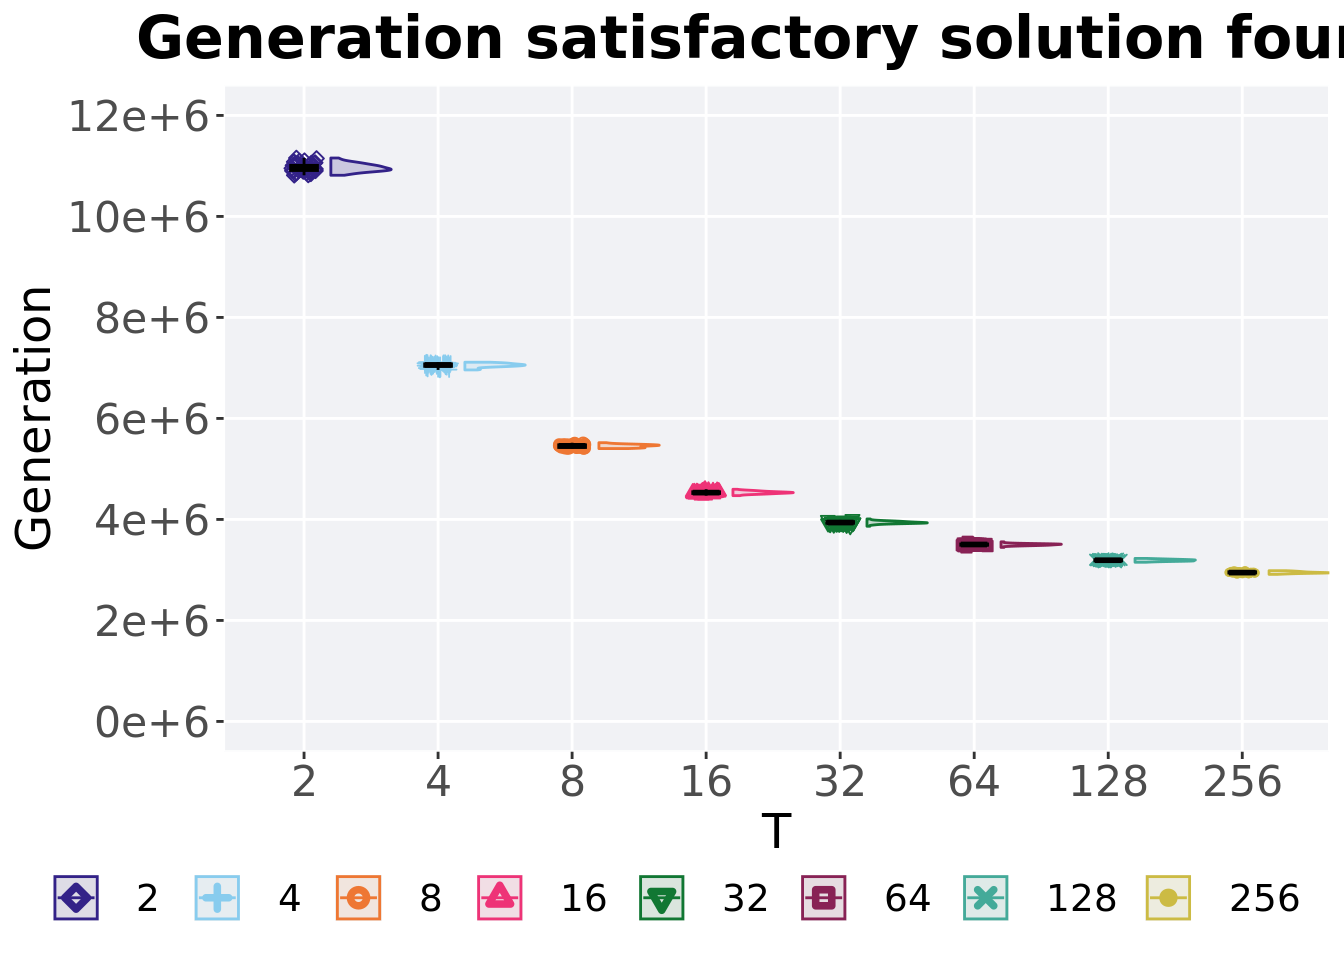
\includegraphics{demo_files/figure-latex/unnamed-chunk-42-1.pdf}

\hypertarget{best-coverage-throughout-1}{%
\subsection{Best coverage throughout}\label{best-coverage-throughout-1}}

Best satisfactory trait coverage throughout 50,000 generations.

\begin{Shaded}
\begin{Highlighting}[]
\NormalTok{nds <-}\StringTok{ }\KeywordTok{filter}\NormalTok{(cc_best, diagnostic }\OperatorTok{==}\StringTok{ 'contradictory_objectives'} \OperatorTok{&}\StringTok{ }\NormalTok{acron }\OperatorTok{==}\StringTok{ 'nds'} \OperatorTok{&}\StringTok{ }\NormalTok{col }\OperatorTok{==}\StringTok{ 'pop_uni_obj'}\NormalTok{)}
\NormalTok{nds}\OperatorTok{$}\StringTok{'Selection}\CharTok{\textbackslash{}n}\StringTok{Scheme'}\NormalTok{ =}\StringTok{ 'Nondominated sorting (nds)'}
\NormalTok{nds =}\StringTok{ }\KeywordTok{subset}\NormalTok{(nds, }\DataTypeTok{select =} \OperatorTok{-}\KeywordTok{c}\NormalTok{(Selection.Scheme) )}

\NormalTok{nfr <-}\StringTok{ }\KeywordTok{read.csv}\NormalTok{(}\StringTok{'./DATA-FINAL/NONDOMINATEDSORTING/best-contradictory_objectives-nondominatedsorting.csv'}\NormalTok{, }\DataTypeTok{header =} \OtherTok{TRUE}\NormalTok{, }\DataTypeTok{stringsAsFactors =} \OtherTok{FALSE}\NormalTok{)}
\NormalTok{nfr}\OperatorTok{$}\NormalTok{acron =}\StringTok{ 'nfr'}
\NormalTok{nfr}\OperatorTok{$}\StringTok{'Selection}\CharTok{\textbackslash{}n}\StringTok{Scheme'}\NormalTok{ =}\StringTok{ 'Nondominated front ranking (nfr)'}
\NormalTok{nfr}\OperatorTok{$}\NormalTok{diagnostic =}\StringTok{ 'contradictory_objectives'}
\NormalTok{nfr <-}\StringTok{ }\KeywordTok{filter}\NormalTok{(nfr, trt }\OperatorTok{==}\StringTok{ }\FloatTok{0.0} \OperatorTok{&}\StringTok{ }\NormalTok{col }\OperatorTok{==}\StringTok{ 'pop_uni_obj'}\NormalTok{)}

\NormalTok{pfs <-}\StringTok{ }\KeywordTok{filter}\NormalTok{(cc_best, diagnostic }\OperatorTok{==}\StringTok{ 'contradictory_objectives'} \OperatorTok{&}\StringTok{ }\NormalTok{acron }\OperatorTok{==}\StringTok{ 'pfs'} \OperatorTok{&}\StringTok{ }\NormalTok{col }\OperatorTok{==}\StringTok{ 'pop_uni_obj'}\NormalTok{)}
\NormalTok{pfs}\OperatorTok{$}\StringTok{'Selection}\CharTok{\textbackslash{}n}\StringTok{Scheme'}\NormalTok{ =}\StringTok{ 'Phenotypic fitness sharing (pfs)'}
\NormalTok{pfs =}\StringTok{ }\KeywordTok{subset}\NormalTok{(pfs, }\DataTypeTok{select =} \OperatorTok{-}\KeywordTok{c}\NormalTok{(Selection.Scheme) )}


\NormalTok{best <-}\StringTok{ }\KeywordTok{rbind}\NormalTok{(nds, nfr, pfs)}
\NormalTok{best}\OperatorTok{$}\StringTok{`}\DataTypeTok{Selection}\CharTok{\textbackslash{}n}\DataTypeTok{Scheme}\StringTok{`}\NormalTok{ <-}\StringTok{ }\KeywordTok{factor}\NormalTok{(best}\OperatorTok{$}\StringTok{`}\DataTypeTok{Selection}\CharTok{\textbackslash{}n}\DataTypeTok{Scheme}\StringTok{`}\NormalTok{, }\DataTypeTok{levels =} \KeywordTok{c}\NormalTok{(}\StringTok{'Nondominated sorting (nds)'}\NormalTok{,}\StringTok{'Nondominated front ranking (nfr)'}\NormalTok{,}\StringTok{'Phenotypic fitness sharing (pfs)'}\NormalTok{))}
\NormalTok{best}\OperatorTok{$}\NormalTok{acron <-}\StringTok{ }\KeywordTok{factor}\NormalTok{(best}\OperatorTok{$}\NormalTok{acron, }\DataTypeTok{levels =} \KeywordTok{c}\NormalTok{(}\StringTok{'nds'}\NormalTok{,}\StringTok{'nfr'}\NormalTok{,}\StringTok{'pfs'}\NormalTok{))}

\NormalTok{plot =}\StringTok{ }\KeywordTok{ggplot}\NormalTok{(best, }\KeywordTok{aes}\NormalTok{(}\DataTypeTok{x =}\NormalTok{ acron, }\DataTypeTok{y =}\NormalTok{ val, }\DataTypeTok{color =}\NormalTok{ acron, }\DataTypeTok{fill =}\NormalTok{ acron, }\DataTypeTok{shape =}\NormalTok{ acron)) }\OperatorTok{+}
\StringTok{  }\KeywordTok{geom_flat_violin}\NormalTok{(}\DataTypeTok{position =} \KeywordTok{position_nudge}\NormalTok{(}\DataTypeTok{x =} \FloatTok{.2}\NormalTok{, }\DataTypeTok{y =} \DecValTok{0}\NormalTok{), }\DataTypeTok{scale =} \StringTok{'width'}\NormalTok{, }\DataTypeTok{alpha =} \FloatTok{0.2}\NormalTok{) }\OperatorTok{+}
\StringTok{  }\KeywordTok{geom_point}\NormalTok{(}\DataTypeTok{position =} \KeywordTok{position_jitter}\NormalTok{(}\DataTypeTok{width =} \FloatTok{.1}\NormalTok{), }\DataTypeTok{size =} \FloatTok{1.5}\NormalTok{, }\DataTypeTok{alpha =} \FloatTok{1.0}\NormalTok{) }\OperatorTok{+}
\StringTok{  }\KeywordTok{geom_boxplot}\NormalTok{(}\DataTypeTok{color =} \StringTok{'black'}\NormalTok{, }\DataTypeTok{width =} \FloatTok{.2}\NormalTok{, }\DataTypeTok{outlier.shape =} \OtherTok{NA}\NormalTok{, }\DataTypeTok{alpha =} \FloatTok{0.0}\NormalTok{) }\OperatorTok{+}
\StringTok{  }\KeywordTok{scale_y_continuous}\NormalTok{(}
    \DataTypeTok{name=}\StringTok{"Coverage"}\NormalTok{,}
    \DataTypeTok{limits=}\KeywordTok{c}\NormalTok{(}\OperatorTok{-}\DecValTok{1}\NormalTok{, }\DecValTok{101}\NormalTok{),}
    \DataTypeTok{breaks=}\KeywordTok{seq}\NormalTok{(}\DecValTok{0}\NormalTok{,}\DecValTok{100}\NormalTok{, }\DecValTok{20}\NormalTok{),}
    \DataTypeTok{labels=}\KeywordTok{c}\NormalTok{(}\StringTok{"0"}\NormalTok{, }\StringTok{"20"}\NormalTok{, }\StringTok{"40"}\NormalTok{, }\StringTok{"60"}\NormalTok{, }\StringTok{"80"}\NormalTok{, }\StringTok{"100"}\NormalTok{)}
\NormalTok{  ) }\OperatorTok{+}
\StringTok{  }\KeywordTok{scale_x_discrete}\NormalTok{(}
    \DataTypeTok{name=}\StringTok{"Scheme"}
\NormalTok{  )}\OperatorTok{+}
\StringTok{  }\KeywordTok{scale_shape_manual}\NormalTok{(}\DataTypeTok{values=}\NormalTok{SHAPE)}\OperatorTok{+}
\StringTok{  }\KeywordTok{scale_colour_manual}\NormalTok{(}\DataTypeTok{values =}\NormalTok{ cb_palette) }\OperatorTok{+}
\StringTok{  }\KeywordTok{scale_fill_manual}\NormalTok{(}\DataTypeTok{values =}\NormalTok{ cb_palette) }\OperatorTok{+}
\StringTok{  }\KeywordTok{coord_flip}\NormalTok{()}\OperatorTok{+}
\StringTok{  }\NormalTok{p_theme}

\KeywordTok{plot_grid}\NormalTok{(}
\NormalTok{  plot }\OperatorTok{+}
\StringTok{    }\KeywordTok{ggtitle}\NormalTok{(}\StringTok{"Best satisfactory trait coverage"}\NormalTok{) }\OperatorTok{+}
\StringTok{    }\KeywordTok{theme}\NormalTok{(}\DataTypeTok{legend.position=}\StringTok{"none"}\NormalTok{),}
\NormalTok{  legend,}
  \DataTypeTok{nrow=}\DecValTok{2}\NormalTok{,}
  \DataTypeTok{rel_heights =} \KeywordTok{c}\NormalTok{(}\DecValTok{2}\NormalTok{,.}\DecValTok{6}\NormalTok{),}
  \DataTypeTok{label_size =}\NormalTok{ TSIZE}
\NormalTok{)}
\end{Highlighting}
\end{Shaded}

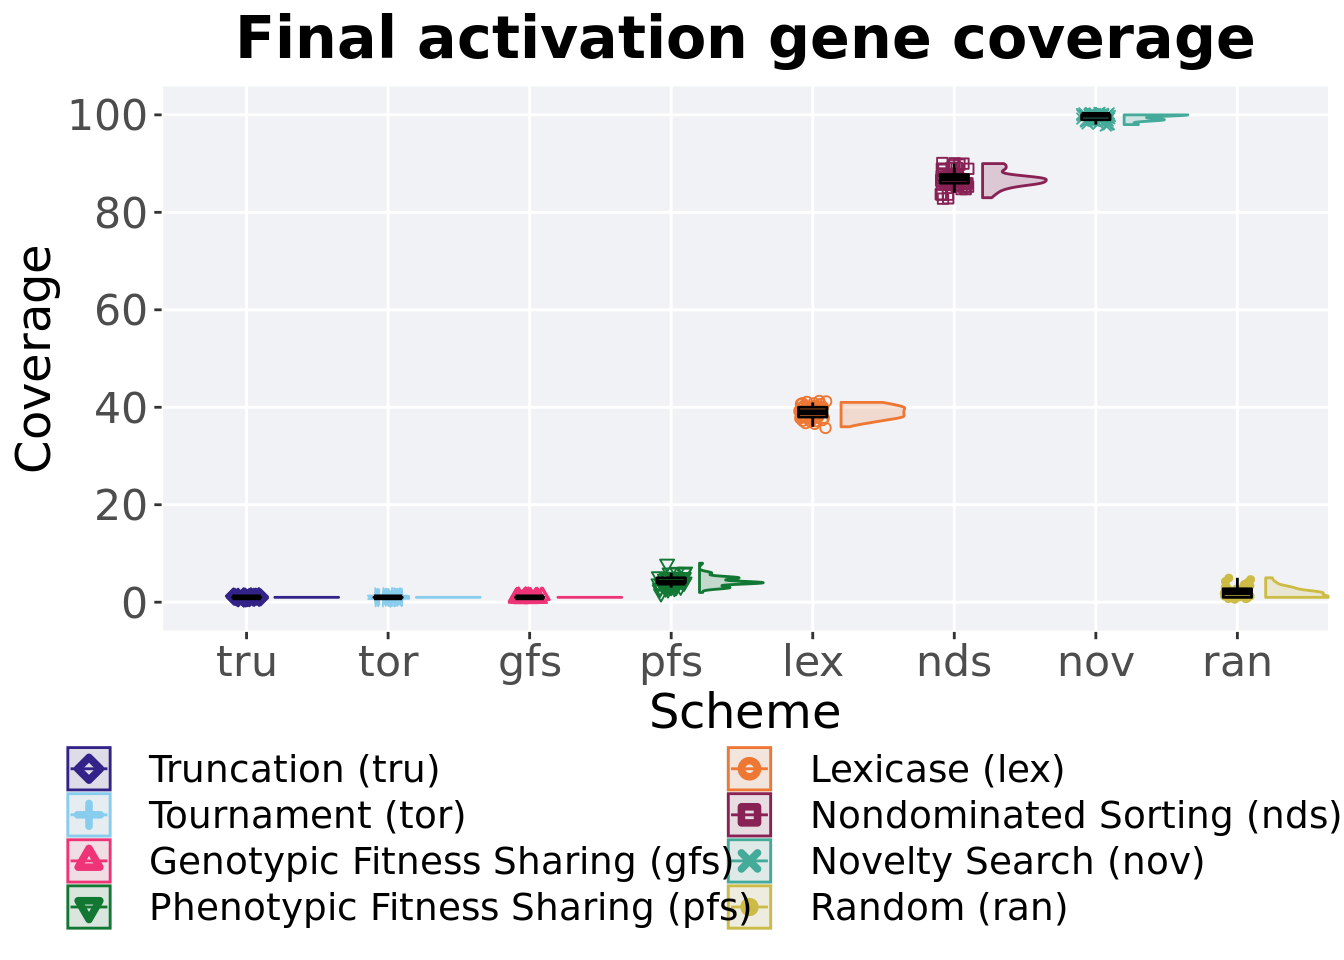
\includegraphics{demo_files/figure-latex/unnamed-chunk-44-1.pdf}

\hypertarget{stats-7}{%
\subsubsection{Stats}\label{stats-7}}

Summary statistics for the best satisfactory trait coverage throughout 50,000 generations.

\begin{Shaded}
\begin{Highlighting}[]
\KeywordTok{group_by}\NormalTok{(best, acron) }\OperatorTok
\StringTok{  }\NormalTok{dplyr}\OperatorTok{::}\KeywordTok{summarise}\NormalTok{(}
    \DataTypeTok{count =} \KeywordTok{n}\NormalTok{(),}
    \DataTypeTok{na_cnt =} \KeywordTok{sum}\NormalTok{(}\KeywordTok{is.na}\NormalTok{(val)),}
    \DataTypeTok{min =} \KeywordTok{min}\NormalTok{(val, }\DataTypeTok{na.rm =} \OtherTok{TRUE}\NormalTok{),}
    \DataTypeTok{median =} \KeywordTok{median}\NormalTok{(val, }\DataTypeTok{na.rm =} \OtherTok{TRUE}\NormalTok{),}
    \DataTypeTok{mean =} \KeywordTok{mean}\NormalTok{(val, }\DataTypeTok{na.rm =} \OtherTok{TRUE}\NormalTok{),}
    \DataTypeTok{max =} \KeywordTok{max}\NormalTok{(val, }\DataTypeTok{na.rm =} \OtherTok{TRUE}\NormalTok{),}
    \DataTypeTok{IQR =} \KeywordTok{IQR}\NormalTok{(val, }\DataTypeTok{na.rm =} \OtherTok{TRUE}\NormalTok{)}
\NormalTok{  )}
\end{Highlighting}
\end{Shaded}

\begin{verbatim}
## # A tibble: 3 x 8
##   acron count na_cnt   min median  mean   max   IQR
##   <fct> <int>  <int> <dbl>  <dbl> <dbl> <dbl> <dbl>
## 1 nds      50      0    87   92   92.6    100  4.75
## 2 nfr      50      0    20   44.5 43.9     56  6.5 
## 3 pfs      50      0     2    4    4.12     8  2
\end{verbatim}

Kruskal--Wallis test provides evidence of difference among best satisfactory trait coverage throughout 50,000 generations

\begin{Shaded}
\begin{Highlighting}[]
\KeywordTok{kruskal.test}\NormalTok{(val }\OperatorTok{~}\StringTok{ }\NormalTok{acron,}\DataTypeTok{data =}\NormalTok{ best)}
\end{Highlighting}
\end{Shaded}

\begin{verbatim}
## 
##  Kruskal-Wallis rank sum test
## 
## data:  val by acron
## Kruskal-Wallis chi-squared = 132.98, df = 2, p-value < 2.2e-16
\end{verbatim}

Results for post-hoc Wilcoxon rank-sum test with a Bonferroni correction on best satisfactory trait coverage throughout 50,000 generations.

\begin{Shaded}
\begin{Highlighting}[]
\KeywordTok{pairwise.wilcox.test}\NormalTok{(}\DataTypeTok{x =}\NormalTok{ best}\OperatorTok{$}\NormalTok{val, }\DataTypeTok{g =}\NormalTok{ best}\OperatorTok{$}\NormalTok{acron, }\DataTypeTok{p.adjust.method =} \StringTok{"bonferroni"}\NormalTok{,}
                     \DataTypeTok{paired =} \OtherTok{FALSE}\NormalTok{, }\DataTypeTok{conf.int =} \OtherTok{FALSE}\NormalTok{, }\DataTypeTok{alternative =} \StringTok{'l'}\NormalTok{)}
\end{Highlighting}
\end{Shaded}

\begin{verbatim}
## 
##  Pairwise comparisons using Wilcoxon rank sum test with continuity correction 
## 
## data:  best$val and best$acron 
## 
##     nds    nfr   
## nfr <2e-16 -     
## pfs <2e-16 <2e-16
## 
## P value adjustment method: bonferroni
\end{verbatim}

\hypertarget{end-of-50000-generations-2}{%
\subsection{End of 50,000 generations}\label{end-of-50000-generations-2}}

Satisfactory trait coverage in the population at the end of 50,000 generations.

\begin{Shaded}
\begin{Highlighting}[]
\NormalTok{nds <-}\StringTok{ }\KeywordTok{filter}\NormalTok{(cc_end, diagnostic }\OperatorTok{==}\StringTok{ 'contradictory_objectives'} \OperatorTok{&}\StringTok{ }\NormalTok{acron }\OperatorTok{==}\StringTok{ 'nds'}\NormalTok{)}
\NormalTok{nds}\OperatorTok{$}\StringTok{'Selection}\CharTok{\textbackslash{}n}\StringTok{Scheme'}\NormalTok{ =}\StringTok{ 'Nondominated sorting (nds)'}

\NormalTok{nfr <-}\StringTok{ }\KeywordTok{read.csv}\NormalTok{(}\StringTok{'./DATA-FINAL/NONDOMINATEDSORTING/over-time-contradictory_objectives-nondominatedsorting.csv'}\NormalTok{, }\DataTypeTok{header =} \OtherTok{TRUE}\NormalTok{, }\DataTypeTok{stringsAsFactors =} \OtherTok{FALSE}\NormalTok{)}
\NormalTok{nfr}\OperatorTok{$}\NormalTok{acron =}\StringTok{ 'nfr'}
\NormalTok{nfr}\OperatorTok{$}\NormalTok{Selection.Scheme =}\StringTok{ 'Nondominated front ranking (nfr)'}
\NormalTok{nfr}\OperatorTok{$}\StringTok{'Selection}\CharTok{\textbackslash{}n}\StringTok{Scheme'}\NormalTok{ =}\StringTok{ 'Nondominated front ranking (nfr)'}
\NormalTok{nfr}\OperatorTok{$}\NormalTok{diagnostic =}\StringTok{ 'contradictory_objectives'}
\NormalTok{nfr <-}\StringTok{ }\KeywordTok{filter}\NormalTok{(nfr, trt }\OperatorTok{==}\StringTok{ }\FloatTok{0.0} \OperatorTok{&}\StringTok{ }\NormalTok{gen }\OperatorTok{==}\StringTok{ }\DecValTok{50000}\NormalTok{)}
\NormalTok{nfr =}\StringTok{ }\KeywordTok{subset}\NormalTok{(nfr, }\DataTypeTok{select =} \OperatorTok{-}\KeywordTok{c}\NormalTok{(Selection.Scheme) )}

\NormalTok{pfs <-}\StringTok{ }\KeywordTok{filter}\NormalTok{(cc_end, diagnostic }\OperatorTok{==}\StringTok{ 'contradictory_objectives'} \OperatorTok{&}\StringTok{ }\NormalTok{acron }\OperatorTok{==}\StringTok{ 'pfs'}\NormalTok{)}
\NormalTok{pfs}\OperatorTok{$}\StringTok{'Selection}\CharTok{\textbackslash{}n}\StringTok{Scheme'}\NormalTok{ =}\StringTok{ 'Phenotypic fitness sharing (pfs)'}

\NormalTok{end <-}\StringTok{ }\KeywordTok{rbind}\NormalTok{(nds, nfr, pfs)}
\NormalTok{end}\OperatorTok{$}\NormalTok{acron <-}\StringTok{ }\KeywordTok{factor}\NormalTok{(end}\OperatorTok{$}\NormalTok{acron, }\DataTypeTok{levels =} \KeywordTok{c}\NormalTok{(}\StringTok{'nds'}\NormalTok{,}\StringTok{'nfr'}\NormalTok{,}\StringTok{'pfs'}\NormalTok{))}

\NormalTok{best =}\StringTok{ }\KeywordTok{ggplot}\NormalTok{(end, }\KeywordTok{aes}\NormalTok{(}\DataTypeTok{x =}\NormalTok{ acron, }\DataTypeTok{y =}\NormalTok{ pop_uni_obj, }\DataTypeTok{color =}\NormalTok{ acron, }\DataTypeTok{fill =}\NormalTok{ acron, }\DataTypeTok{shape =}\NormalTok{ acron)) }\OperatorTok{+}
\StringTok{  }\KeywordTok{geom_flat_violin}\NormalTok{(}\DataTypeTok{position =} \KeywordTok{position_nudge}\NormalTok{(}\DataTypeTok{x =} \FloatTok{.2}\NormalTok{, }\DataTypeTok{y =} \DecValTok{0}\NormalTok{), }\DataTypeTok{scale =} \StringTok{'width'}\NormalTok{, }\DataTypeTok{alpha =} \FloatTok{0.2}\NormalTok{) }\OperatorTok{+}
\StringTok{  }\KeywordTok{geom_point}\NormalTok{(}\DataTypeTok{position =} \KeywordTok{position_jitter}\NormalTok{(}\DataTypeTok{width =} \FloatTok{.1}\NormalTok{), }\DataTypeTok{size =} \FloatTok{1.5}\NormalTok{, }\DataTypeTok{alpha =} \FloatTok{1.0}\NormalTok{) }\OperatorTok{+}
\StringTok{  }\KeywordTok{geom_boxplot}\NormalTok{(}\DataTypeTok{color =} \StringTok{'black'}\NormalTok{, }\DataTypeTok{width =} \FloatTok{.2}\NormalTok{, }\DataTypeTok{outlier.shape =} \OtherTok{NA}\NormalTok{, }\DataTypeTok{alpha =} \FloatTok{0.0}\NormalTok{) }\OperatorTok{+}
\StringTok{  }\KeywordTok{scale_y_continuous}\NormalTok{(}
    \DataTypeTok{name=}\StringTok{"Coverage"}\NormalTok{,}
    \DataTypeTok{limits=}\KeywordTok{c}\NormalTok{(}\OperatorTok{-}\DecValTok{1}\NormalTok{, }\DecValTok{101}\NormalTok{),}
    \DataTypeTok{breaks=}\KeywordTok{seq}\NormalTok{(}\DecValTok{0}\NormalTok{,}\DecValTok{100}\NormalTok{, }\DecValTok{20}\NormalTok{),}
    \DataTypeTok{labels=}\KeywordTok{c}\NormalTok{(}\StringTok{"0"}\NormalTok{, }\StringTok{"20"}\NormalTok{, }\StringTok{"40"}\NormalTok{, }\StringTok{"60"}\NormalTok{, }\StringTok{"80"}\NormalTok{, }\StringTok{"100"}\NormalTok{)}
\NormalTok{  ) }\OperatorTok{+}
\StringTok{  }\KeywordTok{scale_x_discrete}\NormalTok{(}
    \DataTypeTok{name=}\StringTok{"Scheme"}
\NormalTok{  )}\OperatorTok{+}
\StringTok{  }\KeywordTok{scale_shape_manual}\NormalTok{(}\DataTypeTok{values=}\NormalTok{SHAPE)}\OperatorTok{+}
\StringTok{  }\KeywordTok{scale_colour_manual}\NormalTok{(}\DataTypeTok{values =}\NormalTok{ cb_palette) }\OperatorTok{+}
\StringTok{  }\KeywordTok{scale_fill_manual}\NormalTok{(}\DataTypeTok{values =}\NormalTok{ cb_palette) }\OperatorTok{+}
\StringTok{  }\KeywordTok{coord_flip}\NormalTok{()}\OperatorTok{+}
\StringTok{  }\NormalTok{p_theme}

\KeywordTok{plot_grid}\NormalTok{(}
\NormalTok{  best }\OperatorTok{+}
\StringTok{    }\KeywordTok{ggtitle}\NormalTok{(}\StringTok{"Final satisfactory trait coverage"}\NormalTok{) }\OperatorTok{+}
\StringTok{    }\KeywordTok{theme}\NormalTok{(}\DataTypeTok{legend.position=}\StringTok{"none"}\NormalTok{),}
\NormalTok{  legend,}
  \DataTypeTok{nrow=}\DecValTok{2}\NormalTok{,}
  \DataTypeTok{rel_heights =} \KeywordTok{c}\NormalTok{(}\DecValTok{2}\NormalTok{,.}\DecValTok{55}\NormalTok{),}
  \DataTypeTok{label_size =}\NormalTok{ TSIZE}
\NormalTok{)}
\end{Highlighting}
\end{Shaded}

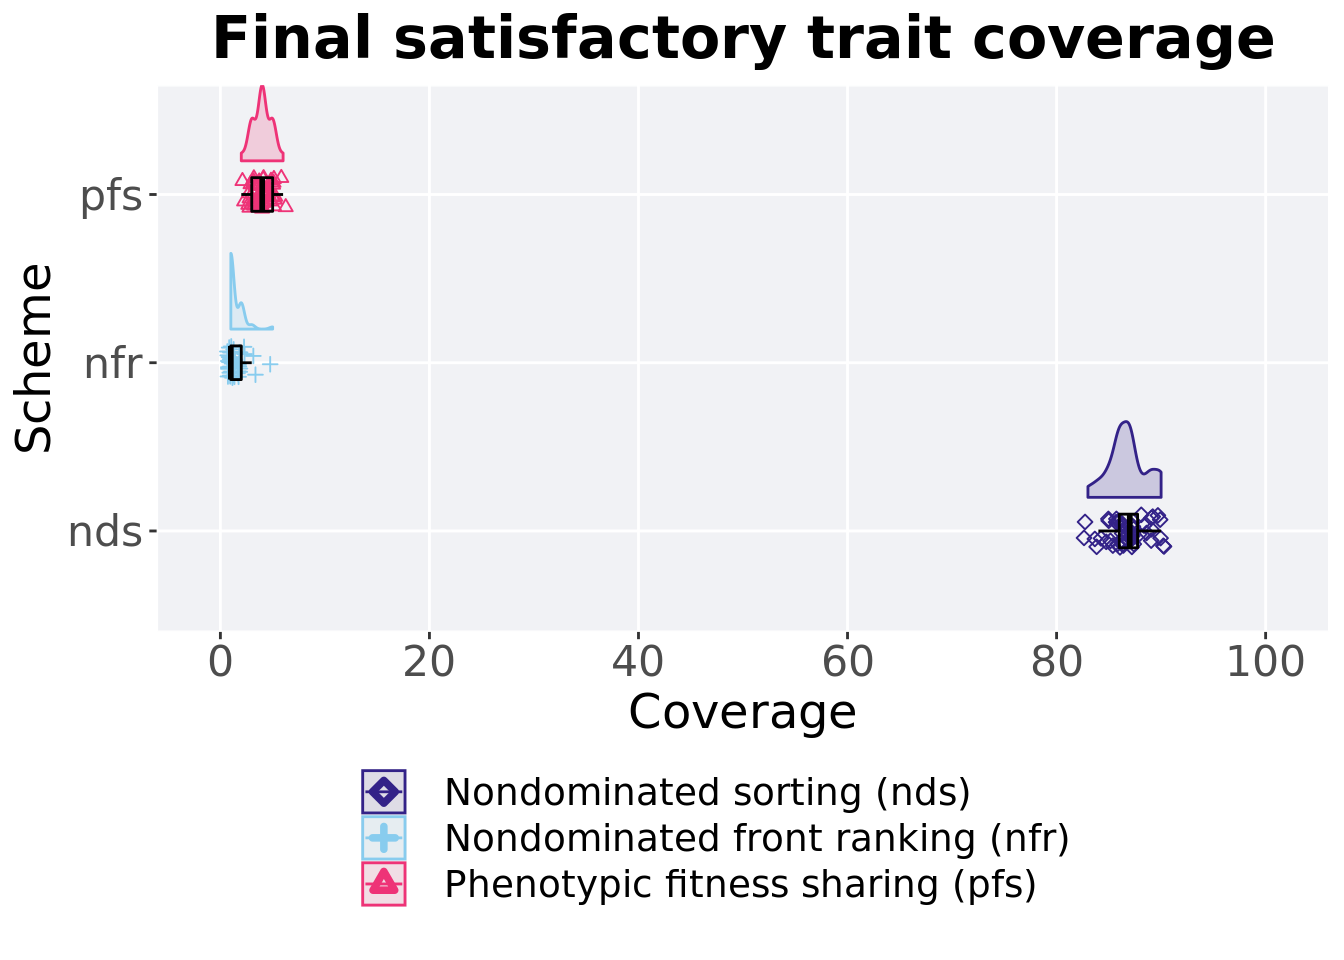
\includegraphics{demo_files/figure-latex/unnamed-chunk-48-1.pdf}

\hypertarget{stats-8}{%
\subsubsection{Stats}\label{stats-8}}

Summary statistics for satisfactory trait coverage in the population at the end of 50,000 generations.

\begin{Shaded}
\begin{Highlighting}[]
\KeywordTok{group_by}\NormalTok{(end, acron) }\OperatorTok
\StringTok{  }\NormalTok{dplyr}\OperatorTok{::}\KeywordTok{summarise}\NormalTok{(}
    \DataTypeTok{count =} \KeywordTok{n}\NormalTok{(),}
    \DataTypeTok{na_cnt =} \KeywordTok{sum}\NormalTok{(}\KeywordTok{is.na}\NormalTok{(pop_uni_obj)),}
    \DataTypeTok{min =} \KeywordTok{min}\NormalTok{(pop_uni_obj, }\DataTypeTok{na.rm =} \OtherTok{TRUE}\NormalTok{),}
    \DataTypeTok{median =} \KeywordTok{median}\NormalTok{(pop_uni_obj, }\DataTypeTok{na.rm =} \OtherTok{TRUE}\NormalTok{),}
    \DataTypeTok{mean =} \KeywordTok{mean}\NormalTok{(pop_uni_obj, }\DataTypeTok{na.rm =} \OtherTok{TRUE}\NormalTok{),}
    \DataTypeTok{max =} \KeywordTok{max}\NormalTok{(pop_uni_obj, }\DataTypeTok{na.rm =} \OtherTok{TRUE}\NormalTok{),}
    \DataTypeTok{IQR =} \KeywordTok{IQR}\NormalTok{(pop_uni_obj, }\DataTypeTok{na.rm =} \OtherTok{TRUE}\NormalTok{)}
\NormalTok{  )}
\end{Highlighting}
\end{Shaded}

\begin{verbatim}
## # A tibble: 3 x 8
##   acron count na_cnt   min median  mean   max   IQR
##   <fct> <int>  <int> <int>  <dbl> <dbl> <int> <dbl>
## 1 nds      50      0    83     87  86.8    90  1.75
## 2 nfr      50      0     1      1   1.4     5  1   
## 3 pfs      50      0     2      4   4       6  2
\end{verbatim}

Kruskal--Wallis test provides evidence of difference among satisfactory trait coverage in the population at the end of 50,000 generations.

\begin{Shaded}
\begin{Highlighting}[]
\KeywordTok{kruskal.test}\NormalTok{(pop_uni_obj }\OperatorTok{~}\StringTok{ }\NormalTok{acron,}\DataTypeTok{data =}\NormalTok{ end)}
\end{Highlighting}
\end{Shaded}

\begin{verbatim}
## 
##  Kruskal-Wallis rank sum test
## 
## data:  pop_uni_obj by acron
## Kruskal-Wallis chi-squared = 131.43, df = 2, p-value < 2.2e-16
\end{verbatim}

Results for post-hoc Wilcoxon rank-sum test with a Bonferroni correction on satisfactory trait coverage in the population at the end of 50,000 generations.

\begin{Shaded}
\begin{Highlighting}[]
\KeywordTok{pairwise.wilcox.test}\NormalTok{(}\DataTypeTok{x =}\NormalTok{ end}\OperatorTok{$}\NormalTok{pop_uni_obj, }\DataTypeTok{g =}\NormalTok{ end}\OperatorTok{$}\NormalTok{acron, }\DataTypeTok{p.adjust.method =} \StringTok{"bonferroni"}\NormalTok{,}
                     \DataTypeTok{paired =} \OtherTok{FALSE}\NormalTok{, }\DataTypeTok{conf.int =} \OtherTok{FALSE}\NormalTok{, }\DataTypeTok{alternative =} \StringTok{'l'}\NormalTok{)}
\end{Highlighting}
\end{Shaded}

\begin{verbatim}
## 
##  Pairwise comparisons using Wilcoxon rank sum test with continuity correction 
## 
## data:  end$pop_uni_obj and end$acron 
## 
##     nds    nfr
## nfr <2e-16 -  
## pfs <2e-16 1  
## 
## P value adjustment method: bonferroni
\end{verbatim}

\hypertarget{multi-path-exploration-results}{%
\chapter{Multi-path exploration results}\label{multi-path-exploration-results}}

Here we present the results for the \textbf{best performances} and \textbf{activation gene coverage} generated by each selection scheme replicate on the contradictory objectives diagnostic.
Best performance found refers to the largest average trait score found in a given population.
Note that activation gene coverage values are gathered at the population-level.
Activation gene coverage refers to the count of unique activation genes in a given population; this gives us a range of integers between 0 and 100.

\hypertarget{analysis-dependencies-3}{%
\section{Analysis dependencies}\label{analysis-dependencies-3}}

\begin{Shaded}
\begin{Highlighting}[]
\KeywordTok{library}\NormalTok{(ggplot2)}
\KeywordTok{library}\NormalTok{(cowplot)}
\KeywordTok{library}\NormalTok{(dplyr)}
\KeywordTok{library}\NormalTok{(PupillometryR)}
\end{Highlighting}
\end{Shaded}

\hypertarget{setup-3}{%
\section{Setup}\label{setup-3}}

These analyses were conducted in the following computing environment:

\begin{Shaded}
\begin{Highlighting}[]
\KeywordTok{print}\NormalTok{(version)}
\end{Highlighting}
\end{Shaded}

\begin{verbatim}
##                _                           
## platform       x86_64-pc-linux-gnu         
## arch           x86_64                      
## os             linux-gnu                   
## system         x86_64, linux-gnu           
## status                                     
## major          4                           
## minor          2.1                         
## year           2022                        
## month          06                          
## day            23                          
## svn rev        82513                       
## language       R                           
## version.string R version 4.2.1 (2022-06-23)
## nickname       Funny-Looking Kid
\end{verbatim}

\hypertarget{performance}{%
\section{Performance}\label{performance}}

Performance analysis.

\hypertarget{over-time}{%
\subsection{Over time}\label{over-time}}

Best performance in a population over time.

\begin{Shaded}
\begin{Highlighting}[]
\NormalTok{multipath_exploration =}\StringTok{ }\KeywordTok{filter}\NormalTok{(cc_over_time, diagnostic }\OperatorTok{==}\StringTok{ 'multipath_exploration'}\NormalTok{)}
\NormalTok{lines =}\StringTok{ }\NormalTok{multipath_exploration }\OperatorTok
\StringTok{        }\KeywordTok{group_by}\NormalTok{(}\StringTok{`}\DataTypeTok{Selection}\CharTok{\textbackslash{}n}\DataTypeTok{Scheme}\StringTok{`}\NormalTok{, gen) }\OperatorTok
\StringTok{          }\NormalTok{dplyr}\OperatorTok{::}\KeywordTok{summarise}\NormalTok{(}
            \DataTypeTok{min =} \KeywordTok{min}\NormalTok{(pop_fit_max),}
            \DataTypeTok{mean =} \KeywordTok{mean}\NormalTok{(pop_fit_max),}
            \DataTypeTok{max =} \KeywordTok{max}\NormalTok{(pop_fit_max)}
\NormalTok{          )}
\end{Highlighting}
\end{Shaded}

\begin{verbatim}
## `summarise()` has grouped output by 'Selection Scheme'. You can override using
## the `.groups` argument.
\end{verbatim}

\begin{Shaded}
\begin{Highlighting}[]
\NormalTok{points =}\StringTok{ }\KeywordTok{filter}\NormalTok{(lines, gen }\OperatorTok\StringTok{ }\DecValTok{2000} \OperatorTok{==}\StringTok{ }\DecValTok{0} \OperatorTok{&}\StringTok{ }\NormalTok{gen }\OperatorTok{!=}\StringTok{ }\DecValTok{0}\NormalTok{)}

\NormalTok{ot =}\StringTok{ }\KeywordTok{ggplot}\NormalTok{(lines, }\KeywordTok{aes}\NormalTok{(}\DataTypeTok{x=}\NormalTok{gen, }\DataTypeTok{y=}\NormalTok{mean }\OperatorTok{/}\StringTok{ }\NormalTok{TRAITS, }\DataTypeTok{group =} \StringTok{`}\DataTypeTok{Selection}\CharTok{\textbackslash{}n}\DataTypeTok{Scheme}\StringTok{`}\NormalTok{, }\DataTypeTok{fill =}\StringTok{`}\DataTypeTok{Selection}\CharTok{\textbackslash{}n}\DataTypeTok{Scheme}\StringTok{`}\NormalTok{, }\DataTypeTok{color =} \StringTok{`}\DataTypeTok{Selection}\CharTok{\textbackslash{}n}\DataTypeTok{Scheme}\StringTok{`}\NormalTok{, }\DataTypeTok{shape =} \StringTok{`}\DataTypeTok{Selection}\CharTok{\textbackslash{}n}\DataTypeTok{Scheme}\StringTok{`}\NormalTok{)) }\OperatorTok{+}
\StringTok{  }\KeywordTok{geom_ribbon}\NormalTok{(}\KeywordTok{aes}\NormalTok{(}\DataTypeTok{ymin =}\NormalTok{ min }\OperatorTok{/}\StringTok{ }\NormalTok{TRAITS, }\DataTypeTok{ymax =}\NormalTok{ max }\OperatorTok{/}\StringTok{ }\NormalTok{TRAITS), }\DataTypeTok{alpha =} \FloatTok{0.1}\NormalTok{) }\OperatorTok{+}
\StringTok{  }\KeywordTok{geom_line}\NormalTok{(}\DataTypeTok{size =} \FloatTok{0.5}\NormalTok{) }\OperatorTok{+}
\StringTok{  }\KeywordTok{geom_point}\NormalTok{(}\DataTypeTok{data =}\NormalTok{ points, }\DataTypeTok{size =} \FloatTok{1.5}\NormalTok{, }\DataTypeTok{stroke =} \FloatTok{2.0}\NormalTok{, }\DataTypeTok{alpha =} \FloatTok{1.0}\NormalTok{) }\OperatorTok{+}
\StringTok{  }\KeywordTok{scale_y_continuous}\NormalTok{(}
    \DataTypeTok{name=}\StringTok{"Average trait score"}\NormalTok{,}
    \DataTypeTok{limits=}\KeywordTok{c}\NormalTok{(}\OperatorTok{-}\DecValTok{1}\NormalTok{, }\DecValTok{101}\NormalTok{),}
    \DataTypeTok{breaks=}\KeywordTok{seq}\NormalTok{(}\DecValTok{0}\NormalTok{,}\DecValTok{100}\NormalTok{, }\DecValTok{20}\NormalTok{),}
    \DataTypeTok{labels=}\KeywordTok{c}\NormalTok{(}\StringTok{"0"}\NormalTok{, }\StringTok{"20"}\NormalTok{, }\StringTok{"40"}\NormalTok{, }\StringTok{"60"}\NormalTok{, }\StringTok{"80"}\NormalTok{, }\StringTok{"100"}\NormalTok{)}
\NormalTok{  ) }\OperatorTok{+}
\StringTok{  }\KeywordTok{scale_x_continuous}\NormalTok{(}
    \DataTypeTok{name=}\StringTok{"Generations"}\NormalTok{,}
    \DataTypeTok{limits=}\KeywordTok{c}\NormalTok{(}\DecValTok{0}\NormalTok{, }\DecValTok{50000}\NormalTok{),}
    \DataTypeTok{breaks=}\KeywordTok{c}\NormalTok{(}\DecValTok{0}\NormalTok{, }\DecValTok{10000}\NormalTok{, }\DecValTok{20000}\NormalTok{, }\DecValTok{30000}\NormalTok{, }\DecValTok{40000}\NormalTok{, }\DecValTok{50000}\NormalTok{),}
    \DataTypeTok{labels=}\KeywordTok{c}\NormalTok{(}\StringTok{"0e+6"}\NormalTok{, }\StringTok{"1e+6"}\NormalTok{, }\StringTok{"2e+6"}\NormalTok{, }\StringTok{"3e+6"}\NormalTok{, }\StringTok{"4e+6"}\NormalTok{, }\StringTok{"5e+6"}\NormalTok{)}

\NormalTok{  ) }\OperatorTok{+}
\StringTok{  }\KeywordTok{scale_shape_manual}\NormalTok{(}\DataTypeTok{values=}\NormalTok{SHAPE)}\OperatorTok{+}
\StringTok{  }\KeywordTok{scale_colour_manual}\NormalTok{(}\DataTypeTok{values =}\NormalTok{ cb_palette) }\OperatorTok{+}
\StringTok{  }\KeywordTok{scale_fill_manual}\NormalTok{(}\DataTypeTok{values =}\NormalTok{ cb_palette) }\OperatorTok{+}
\StringTok{  }\KeywordTok{ggtitle}\NormalTok{(}\StringTok{"Best performance over time"}\NormalTok{) }\OperatorTok{+}
\StringTok{  }\NormalTok{p_theme}\OperatorTok{+}
\StringTok{    }\KeywordTok{guides}\NormalTok{(}
    \DataTypeTok{shape=}\KeywordTok{guide_legend}\NormalTok{(}\DataTypeTok{ncol=}\DecValTok{2}\NormalTok{, }\DataTypeTok{title.position =} \StringTok{"bottom"}\NormalTok{),}
    \DataTypeTok{color=}\KeywordTok{guide_legend}\NormalTok{(}\DataTypeTok{ncol=}\DecValTok{2}\NormalTok{, }\DataTypeTok{title.position =} \StringTok{"bottom"}\NormalTok{),}
    \DataTypeTok{fill=}\KeywordTok{guide_legend}\NormalTok{(}\DataTypeTok{ncol=}\DecValTok{2}\NormalTok{, }\DataTypeTok{title.position =} \StringTok{"bottom"}\NormalTok{)}
\NormalTok{  ) }\OperatorTok{+}
\StringTok{  }\KeywordTok{theme}\NormalTok{(}
    \DataTypeTok{legend.position =} \StringTok{"bottom"}\NormalTok{,}
    \DataTypeTok{legend.box=}\StringTok{"verticle"}\NormalTok{,}
    \DataTypeTok{legend.justification=}\StringTok{"center"}\NormalTok{,}
    \DataTypeTok{legend.title=}\KeywordTok{element_blank}\NormalTok{()}
\NormalTok{  )}

\NormalTok{ot}
\end{Highlighting}
\end{Shaded}

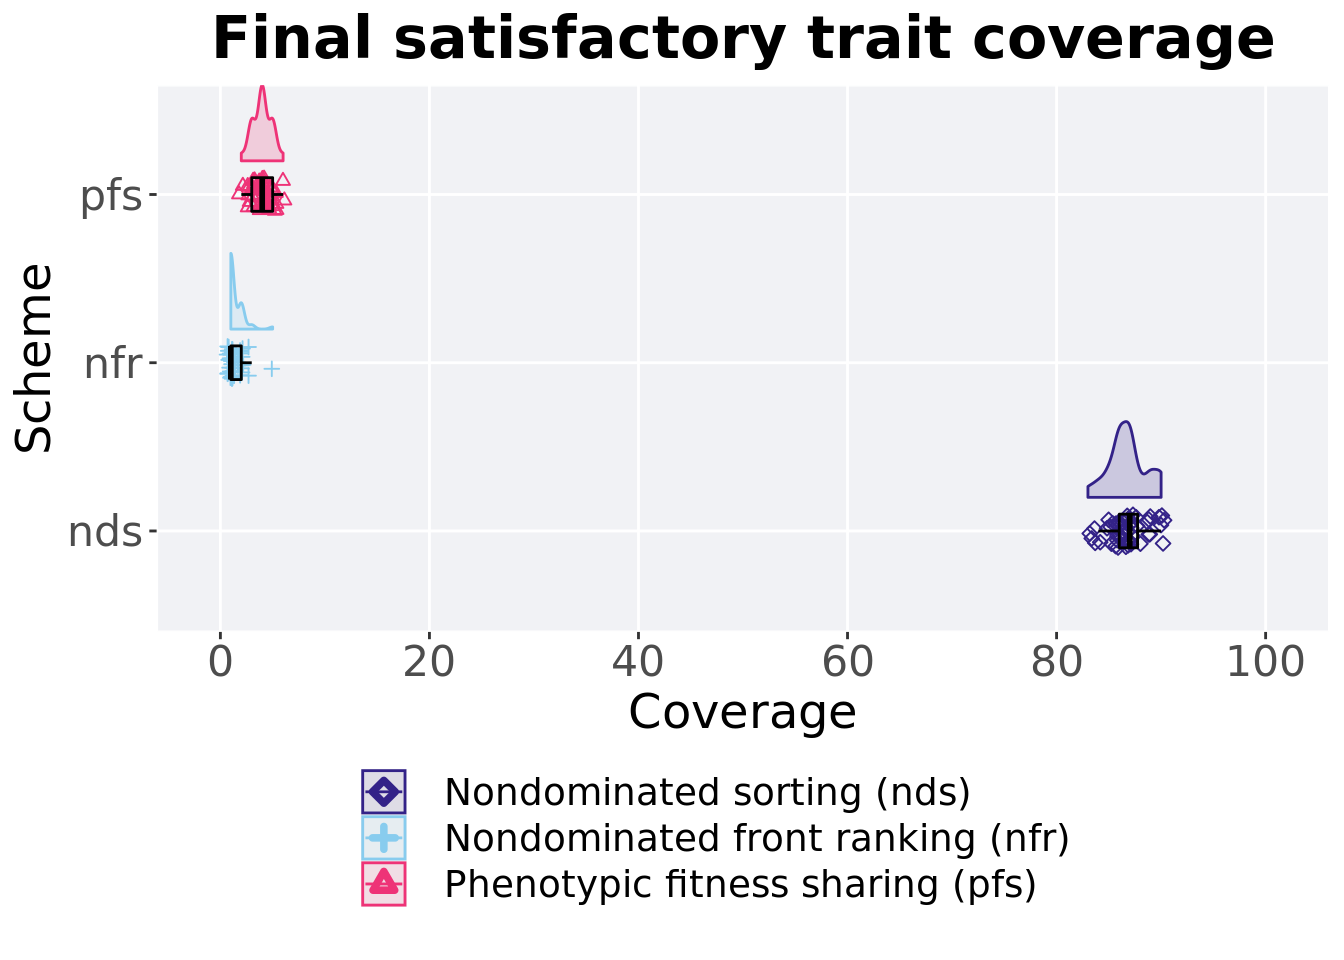
\includegraphics{demo_files/figure-latex/unnamed-chunk-54-1.pdf}

\hypertarget{best-performance-throughout-2}{%
\subsection{Best performance throughout}\label{best-performance-throughout-2}}

Best performance throughout 50,000 generations.

\begin{Shaded}
\begin{Highlighting}[]
\NormalTok{best =}\StringTok{ }\KeywordTok{filter}\NormalTok{(cc_best, col }\OperatorTok{==}\StringTok{ 'pop_fit_max'} \OperatorTok{&}\StringTok{ }\NormalTok{diagnostic }\OperatorTok{==}\StringTok{ 'multipath_exploration'}\NormalTok{)}
\NormalTok{plot =}\StringTok{ }\KeywordTok{ggplot}\NormalTok{(best, }\KeywordTok{aes}\NormalTok{(}\DataTypeTok{x =}\NormalTok{ acron, }\DataTypeTok{y =}\NormalTok{ val }\OperatorTok{/}\StringTok{ }\NormalTok{TRAITS, }\DataTypeTok{color =}\NormalTok{ acron, }\DataTypeTok{fill =}\NormalTok{ acron, }\DataTypeTok{shape =}\NormalTok{ acron)) }\OperatorTok{+}
\StringTok{  }\KeywordTok{geom_flat_violin}\NormalTok{(}\DataTypeTok{position =} \KeywordTok{position_nudge}\NormalTok{(}\DataTypeTok{x =} \FloatTok{.2}\NormalTok{, }\DataTypeTok{y =} \DecValTok{0}\NormalTok{), }\DataTypeTok{scale =} \StringTok{'width'}\NormalTok{, }\DataTypeTok{alpha =} \FloatTok{0.2}\NormalTok{) }\OperatorTok{+}
\StringTok{  }\KeywordTok{geom_point}\NormalTok{(}\DataTypeTok{position =} \KeywordTok{position_jitter}\NormalTok{(}\DataTypeTok{width =} \FloatTok{.1}\NormalTok{), }\DataTypeTok{size =} \FloatTok{1.5}\NormalTok{, }\DataTypeTok{alpha =} \FloatTok{1.0}\NormalTok{) }\OperatorTok{+}
\StringTok{  }\KeywordTok{geom_boxplot}\NormalTok{(}\DataTypeTok{color =} \StringTok{'black'}\NormalTok{, }\DataTypeTok{width =} \FloatTok{.2}\NormalTok{, }\DataTypeTok{outlier.shape =} \OtherTok{NA}\NormalTok{, }\DataTypeTok{alpha =} \FloatTok{0.0}\NormalTok{) }\OperatorTok{+}
\StringTok{  }\KeywordTok{scale_y_continuous}\NormalTok{(}
    \DataTypeTok{name=}\StringTok{"Average trait score"}\NormalTok{,}
    \DataTypeTok{limits=}\KeywordTok{c}\NormalTok{(}\OperatorTok{-}\DecValTok{1}\NormalTok{, }\DecValTok{101}\NormalTok{),}
    \DataTypeTok{breaks=}\KeywordTok{seq}\NormalTok{(}\DecValTok{0}\NormalTok{,}\DecValTok{100}\NormalTok{, }\DecValTok{20}\NormalTok{),}
    \DataTypeTok{labels=}\KeywordTok{c}\NormalTok{(}\StringTok{"0"}\NormalTok{, }\StringTok{"20"}\NormalTok{, }\StringTok{"40"}\NormalTok{, }\StringTok{"60"}\NormalTok{, }\StringTok{"80"}\NormalTok{, }\StringTok{"100"}\NormalTok{)}
\NormalTok{  ) }\OperatorTok{+}
\StringTok{  }\KeywordTok{scale_x_discrete}\NormalTok{(}
    \DataTypeTok{name=}\StringTok{"Scheme"}
\NormalTok{  )}\OperatorTok{+}
\StringTok{  }\KeywordTok{scale_shape_manual}\NormalTok{(}\DataTypeTok{values=}\NormalTok{SHAPE)}\OperatorTok{+}
\StringTok{  }\KeywordTok{scale_colour_manual}\NormalTok{(}\DataTypeTok{values =}\NormalTok{ cb_palette) }\OperatorTok{+}
\StringTok{  }\KeywordTok{scale_fill_manual}\NormalTok{(}\DataTypeTok{values =}\NormalTok{ cb_palette) }\OperatorTok{+}
\StringTok{  }\NormalTok{p_theme}

\KeywordTok{plot_grid}\NormalTok{(}
\NormalTok{  plot }\OperatorTok{+}
\StringTok{    }\KeywordTok{ggtitle}\NormalTok{(}\StringTok{"Best performance throughout"}\NormalTok{) }\OperatorTok{+}
\StringTok{    }\KeywordTok{theme}\NormalTok{(}\DataTypeTok{legend.position=}\StringTok{"none"}\NormalTok{),}
\NormalTok{  legend,}
  \DataTypeTok{nrow=}\DecValTok{2}\NormalTok{,}
  \DataTypeTok{rel_heights =} \KeywordTok{c}\NormalTok{(}\DecValTok{2}\NormalTok{,.}\DecValTok{55}\NormalTok{),}
  \DataTypeTok{label_size =}\NormalTok{ TSIZE}
\NormalTok{)}
\end{Highlighting}
\end{Shaded}

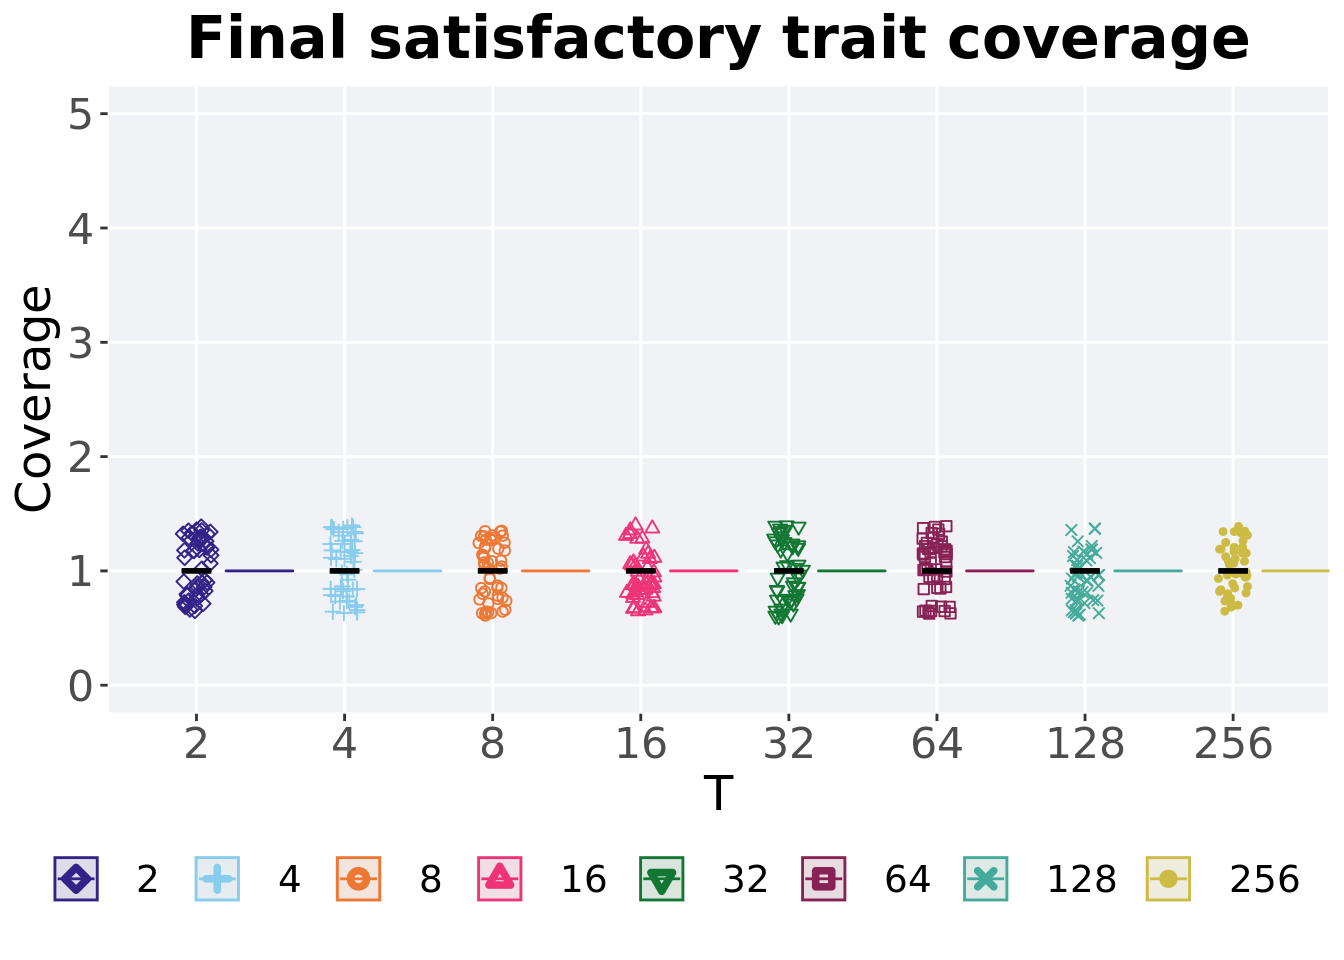
\includegraphics{demo_files/figure-latex/unnamed-chunk-56-1.pdf}

\hypertarget{stats-9}{%
\subsubsection{Stats}\label{stats-9}}

Summary statistics for the best performance throughout 50,000 generations.

\begin{Shaded}
\begin{Highlighting}[]
\NormalTok{best}\OperatorTok{$}\NormalTok{acron <-}\StringTok{ }\KeywordTok{factor}\NormalTok{(best}\OperatorTok{$}\NormalTok{acron, }\DataTypeTok{levels =} \KeywordTok{c}\NormalTok{(}\StringTok{'lex'}\NormalTok{,}\StringTok{'tor'}\NormalTok{,}\StringTok{'tru'}\NormalTok{,}\StringTok{'nds'}\NormalTok{,}\StringTok{'gfs'}\NormalTok{,}\StringTok{'pfs'}\NormalTok{,}\StringTok{'nov'}\NormalTok{,}\StringTok{'ran'}\NormalTok{))}
\KeywordTok{group_by}\NormalTok{(best, acron) }\OperatorTok
\StringTok{  }\NormalTok{dplyr}\OperatorTok{::}\KeywordTok{summarise}\NormalTok{(}
    \DataTypeTok{count =} \KeywordTok{n}\NormalTok{(),}
    \DataTypeTok{na_cnt =} \KeywordTok{sum}\NormalTok{(}\KeywordTok{is.na}\NormalTok{(val)),}
    \DataTypeTok{min =} \KeywordTok{min}\NormalTok{(val, }\DataTypeTok{na.rm =} \OtherTok{TRUE}\NormalTok{),}
    \DataTypeTok{median =} \KeywordTok{median}\NormalTok{(val, }\DataTypeTok{na.rm =} \OtherTok{TRUE}\NormalTok{),}
    \DataTypeTok{mean =} \KeywordTok{mean}\NormalTok{(val, }\DataTypeTok{na.rm =} \OtherTok{TRUE}\NormalTok{),}
    \DataTypeTok{max =} \KeywordTok{max}\NormalTok{(val, }\DataTypeTok{na.rm =} \OtherTok{TRUE}\NormalTok{),}
    \DataTypeTok{IQR =} \KeywordTok{IQR}\NormalTok{(val, }\DataTypeTok{na.rm =} \OtherTok{TRUE}\NormalTok{)}
\NormalTok{  )}
\end{Highlighting}
\end{Shaded}

\begin{verbatim}
## # A tibble: 8 x 8
##   acron count na_cnt    min median  mean   max    IQR
##   <fct> <int>  <int>  <dbl>  <dbl> <dbl> <dbl>  <dbl>
## 1 lex      50      0 8119.   9221. 9165. 9810.  499. 
## 2 tor      50      0  500    6649. 5873. 9894. 4673. 
## 3 tru      50      0  500    4900. 5156. 9897. 3849. 
## 4 nds      50      0 1692.   1971. 1957. 2244.  171. 
## 5 gfs      50      0  400.   2045. 1921. 2283.  152. 
## 6 pfs      50      0  583.   1336. 1274. 1456.  177. 
## 7 nov      50      0  263.    384.  389.  599.   86.5
## 8 ran      50      0   90.1   121.  124.  199.   29.9
\end{verbatim}

Kruskal--Wallis test provides evidence of difference among best performances throughout 50,000 generations.

\begin{Shaded}
\begin{Highlighting}[]
\KeywordTok{kruskal.test}\NormalTok{(val }\OperatorTok{~}\StringTok{ }\NormalTok{acron,}\DataTypeTok{data =}\NormalTok{ best)}
\end{Highlighting}
\end{Shaded}

\begin{verbatim}
## 
##  Kruskal-Wallis rank sum test
## 
## data:  val by acron
## Kruskal-Wallis chi-squared = 353.07, df = 7, p-value < 2.2e-16
\end{verbatim}

Results for post-hoc Wilcoxon rank-sum test with a Bonferroni correction on best performance throughout 50,000 generations.

\begin{Shaded}
\begin{Highlighting}[]
\KeywordTok{pairwise.wilcox.test}\NormalTok{(}\DataTypeTok{x =}\NormalTok{ best}\OperatorTok{$}\NormalTok{val, }\DataTypeTok{g =}\NormalTok{ best}\OperatorTok{$}\NormalTok{acron, }\DataTypeTok{p.adjust.method =} \StringTok{"bonferroni"}\NormalTok{,}
                     \DataTypeTok{paired =} \OtherTok{FALSE}\NormalTok{, }\DataTypeTok{conf.int =} \OtherTok{FALSE}\NormalTok{, }\DataTypeTok{alternative =} \StringTok{'l'}\NormalTok{)}
\end{Highlighting}
\end{Shaded}

\begin{verbatim}
## 
##  Pairwise comparisons using Wilcoxon rank sum test with continuity correction 
## 
## data:  best$val and best$acron 
## 
##     lex     tor     tru     nds     gfs     pfs     nov    
## tor 2.0e-11 -       -       -       -       -       -      
## tru 7.8e-11 1       -       -       -       -       -      
## nds < 2e-16 2.7e-10 2.2e-10 -       -       -       -      
## gfs < 2e-16 3.6e-10 3.8e-10 1       -       -       -      
## pfs < 2e-16 3.5e-13 4.1e-13 < 2e-16 2.5e-11 -       -      
## nov < 2e-16 < 2e-16 < 2e-16 < 2e-16 2.7e-16 < 2e-16 -      
## ran < 2e-16 < 2e-16 < 2e-16 < 2e-16 < 2e-16 < 2e-16 < 2e-16
## 
## P value adjustment method: bonferroni
\end{verbatim}

\hypertarget{end-of-50000-generations-3}{%
\subsection{End of 50,000 generations}\label{end-of-50000-generations-3}}

Best performance in the population at the end of 50,000 generations.

\begin{Shaded}
\begin{Highlighting}[]
\NormalTok{end =}\StringTok{ }\KeywordTok{filter}\NormalTok{(cc_end, diagnostic }\OperatorTok{==}\StringTok{ 'multipath_exploration'}\NormalTok{)}
\NormalTok{plot =}\StringTok{ }\KeywordTok{ggplot}\NormalTok{(end, }\KeywordTok{aes}\NormalTok{(}\DataTypeTok{x =}\NormalTok{ acron, }\DataTypeTok{y =}\NormalTok{ pop_fit_max }\OperatorTok{/}\StringTok{ }\NormalTok{TRAITS, }\DataTypeTok{color =}\NormalTok{ acron, }\DataTypeTok{fill =}\NormalTok{ acron, }\DataTypeTok{shape =}\NormalTok{ acron)) }\OperatorTok{+}
\StringTok{  }\KeywordTok{geom_flat_violin}\NormalTok{(}\DataTypeTok{position =} \KeywordTok{position_nudge}\NormalTok{(}\DataTypeTok{x =} \FloatTok{.2}\NormalTok{, }\DataTypeTok{y =} \DecValTok{0}\NormalTok{), }\DataTypeTok{scale =} \StringTok{'width'}\NormalTok{, }\DataTypeTok{alpha =} \FloatTok{0.2}\NormalTok{) }\OperatorTok{+}
\StringTok{  }\KeywordTok{geom_point}\NormalTok{(}\DataTypeTok{position =} \KeywordTok{position_jitter}\NormalTok{(}\DataTypeTok{width =} \FloatTok{.1}\NormalTok{), }\DataTypeTok{size =} \FloatTok{1.5}\NormalTok{, }\DataTypeTok{alpha =} \FloatTok{1.0}\NormalTok{) }\OperatorTok{+}
\StringTok{  }\KeywordTok{geom_boxplot}\NormalTok{(}\DataTypeTok{color =} \StringTok{'black'}\NormalTok{, }\DataTypeTok{width =} \FloatTok{.2}\NormalTok{, }\DataTypeTok{outlier.shape =} \OtherTok{NA}\NormalTok{, }\DataTypeTok{alpha =} \FloatTok{0.0}\NormalTok{) }\OperatorTok{+}
\StringTok{  }\KeywordTok{scale_y_continuous}\NormalTok{(}
    \DataTypeTok{name=}\StringTok{"Average trait score"}\NormalTok{,}
    \DataTypeTok{limits=}\KeywordTok{c}\NormalTok{(}\OperatorTok{-}\DecValTok{1}\NormalTok{, }\DecValTok{101}\NormalTok{),}
    \DataTypeTok{breaks=}\KeywordTok{seq}\NormalTok{(}\DecValTok{0}\NormalTok{,}\DecValTok{100}\NormalTok{, }\DecValTok{20}\NormalTok{),}
    \DataTypeTok{labels=}\KeywordTok{c}\NormalTok{(}\StringTok{"0"}\NormalTok{, }\StringTok{"20"}\NormalTok{, }\StringTok{"40"}\NormalTok{, }\StringTok{"60"}\NormalTok{, }\StringTok{"80"}\NormalTok{, }\StringTok{"100"}\NormalTok{)}
\NormalTok{  ) }\OperatorTok{+}
\StringTok{  }\KeywordTok{scale_x_discrete}\NormalTok{(}
    \DataTypeTok{name=}\StringTok{"Scheme"}
\NormalTok{  )}\OperatorTok{+}
\StringTok{  }\KeywordTok{scale_shape_manual}\NormalTok{(}\DataTypeTok{values=}\NormalTok{SHAPE)}\OperatorTok{+}
\StringTok{  }\KeywordTok{scale_colour_manual}\NormalTok{(}\DataTypeTok{values =}\NormalTok{ cb_palette) }\OperatorTok{+}
\StringTok{  }\KeywordTok{scale_fill_manual}\NormalTok{(}\DataTypeTok{values =}\NormalTok{ cb_palette) }\OperatorTok{+}
\StringTok{  }\NormalTok{p_theme}

\KeywordTok{plot_grid}\NormalTok{(}
\NormalTok{  plot }\OperatorTok{+}
\StringTok{  }\KeywordTok{ggtitle}\NormalTok{(}\StringTok{"Best performance over time"}\NormalTok{) }\OperatorTok{+}
\StringTok{    }\KeywordTok{theme}\NormalTok{(}\DataTypeTok{legend.position=}\StringTok{"none"}\NormalTok{),}
\NormalTok{  legend,}
  \DataTypeTok{nrow=}\DecValTok{2}\NormalTok{,}
  \DataTypeTok{rel_heights =} \KeywordTok{c}\NormalTok{(}\DecValTok{2}\NormalTok{,.}\DecValTok{55}\NormalTok{),}
  \DataTypeTok{label_size =}\NormalTok{ TSIZE}
\NormalTok{)}
\end{Highlighting}
\end{Shaded}

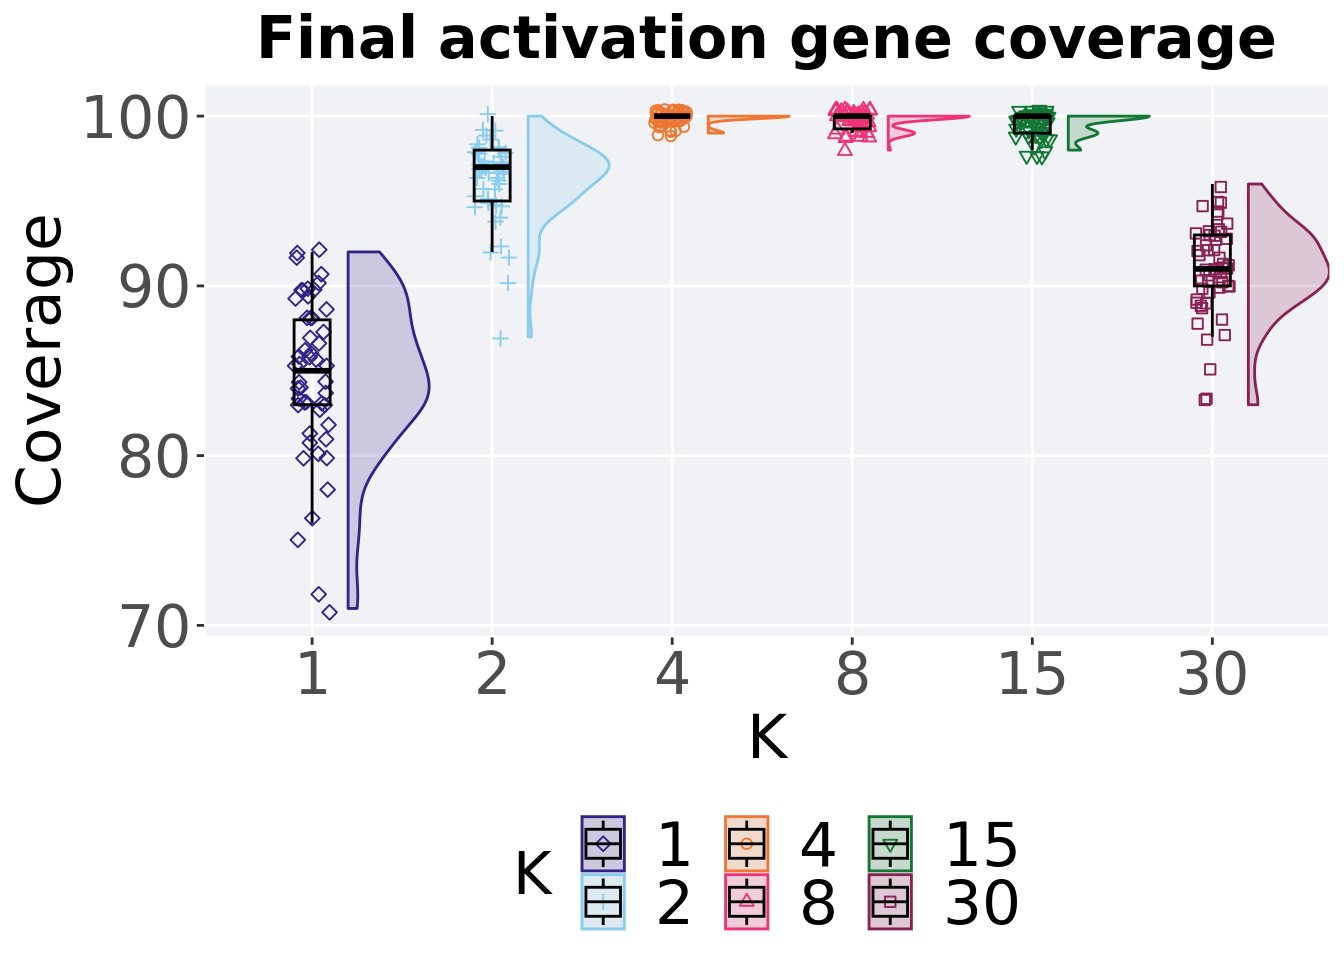
\includegraphics{demo_files/figure-latex/unnamed-chunk-60-1.pdf}

\hypertarget{stats-10}{%
\subsubsection{Stats}\label{stats-10}}

Summary statistics for best performance in the population at the end of 50,000 generations.

\begin{Shaded}
\begin{Highlighting}[]
\NormalTok{end}\OperatorTok{$}\NormalTok{acron <-}\StringTok{ }\KeywordTok{factor}\NormalTok{(end}\OperatorTok{$}\NormalTok{acron, }\DataTypeTok{levels =} \KeywordTok{c}\NormalTok{(}\StringTok{'lex'}\NormalTok{,}\StringTok{'tor'}\NormalTok{,}\StringTok{'tru'}\NormalTok{,}\StringTok{'nds'}\NormalTok{,}\StringTok{'gfs'}\NormalTok{,}\StringTok{'pfs'}\NormalTok{,}\StringTok{'nov'}\NormalTok{,}\StringTok{'ran'}\NormalTok{))}
\KeywordTok{group_by}\NormalTok{(end, acron) }\OperatorTok
\StringTok{  }\NormalTok{dplyr}\OperatorTok{::}\KeywordTok{summarise}\NormalTok{(}
    \DataTypeTok{count =} \KeywordTok{n}\NormalTok{(),}
    \DataTypeTok{na_cnt =} \KeywordTok{sum}\NormalTok{(}\KeywordTok{is.na}\NormalTok{(pop_fit_max)),}
    \DataTypeTok{min =} \KeywordTok{min}\NormalTok{(pop_fit_max, }\DataTypeTok{na.rm =} \OtherTok{TRUE}\NormalTok{),}
    \DataTypeTok{median =} \KeywordTok{median}\NormalTok{(pop_fit_max, }\DataTypeTok{na.rm =} \OtherTok{TRUE}\NormalTok{),}
    \DataTypeTok{mean =} \KeywordTok{mean}\NormalTok{(pop_fit_max, }\DataTypeTok{na.rm =} \OtherTok{TRUE}\NormalTok{),}
    \DataTypeTok{max =} \KeywordTok{max}\NormalTok{(pop_fit_max, }\DataTypeTok{na.rm =} \OtherTok{TRUE}\NormalTok{),}
    \DataTypeTok{IQR =} \KeywordTok{IQR}\NormalTok{(pop_fit_max, }\DataTypeTok{na.rm =} \OtherTok{TRUE}\NormalTok{)}
\NormalTok{  )}
\end{Highlighting}
\end{Shaded}

\begin{verbatim}
## # A tibble: 8 x 8
##   acron count na_cnt    min median   mean   max    IQR
##   <fct> <int>  <int>  <dbl>  <dbl>  <dbl> <dbl>  <dbl>
## 1 lex      50      0 7559.  9074.  8969.  9810.  589. 
## 2 tor      50      0  500   6649.  5873.  9894. 4673. 
## 3 tru      50      0  500   4900.  5156.  9897. 3849. 
## 4 nds      50      0 1232.  1800.  1791.  2244.  206. 
## 5 gfs      50      0  399.  2041.  1916.  2283.  153. 
## 6 pfs      50      0  570.  1333.  1268.  1448.  174. 
## 7 nov      50      0  210.   336.   349.   568.   73.0
## 8 ran      50      0   55.0   79.9   87.0  183.   30.4
\end{verbatim}

Kruskal--Wallis test provides evidence of difference among best performance in the population at the end of 50,000 generations.

\begin{Shaded}
\begin{Highlighting}[]
\KeywordTok{kruskal.test}\NormalTok{(pop_fit_max }\OperatorTok{~}\StringTok{ }\NormalTok{acron,}\DataTypeTok{data =}\NormalTok{ end)}
\end{Highlighting}
\end{Shaded}

\begin{verbatim}
## 
##  Kruskal-Wallis rank sum test
## 
## data:  pop_fit_max by acron
## Kruskal-Wallis chi-squared = 353.68, df = 7, p-value < 2.2e-16
\end{verbatim}

Results for post-hoc Wilcoxon rank-sum test with a Bonferroni correction on best performance in the population at the end of 50,000 generations.

\begin{Shaded}
\begin{Highlighting}[]
\KeywordTok{pairwise.wilcox.test}\NormalTok{(}\DataTypeTok{x =}\NormalTok{ end}\OperatorTok{$}\NormalTok{pop_fit_max, }\DataTypeTok{g =}\NormalTok{ end}\OperatorTok{$}\NormalTok{acron, }\DataTypeTok{p.adjust.method =} \StringTok{"bonferroni"}\NormalTok{,}
                     \DataTypeTok{paired =} \OtherTok{FALSE}\NormalTok{, }\DataTypeTok{conf.int =} \OtherTok{FALSE}\NormalTok{, }\DataTypeTok{alternative =} \StringTok{'l'}\NormalTok{)}
\end{Highlighting}
\end{Shaded}

\begin{verbatim}
## 
##  Pairwise comparisons using Wilcoxon rank sum test with continuity correction 
## 
## data:  end$pop_fit_max and end$acron 
## 
##     lex     tor     tru     nds     gfs     pfs     nov    
## tor 6.6e-10 -       -       -       -       -       -      
## tru 6.0e-10 1       -       -       -       -       -      
## nds < 2e-16 8.2e-11 4.8e-11 -       -       -       -      
## gfs < 2e-16 3.4e-10 3.6e-10 1       -       -       -      
## pfs < 2e-16 3.2e-13 4.1e-13 8.9e-16 2.5e-11 -       -      
## nov < 2e-16 < 2e-16 < 2e-16 < 2e-16 < 2e-16 < 2e-16 -      
## ran < 2e-16 < 2e-16 < 2e-16 < 2e-16 < 2e-16 < 2e-16 < 2e-16
## 
## P value adjustment method: bonferroni
\end{verbatim}

\hypertarget{activation-gene-coverage-1}{%
\section{Activation gene coverage}\label{activation-gene-coverage-1}}

Activation gene coverage analysis.

\hypertarget{over-time-coverage-1}{%
\subsection{Over time coverage}\label{over-time-coverage-1}}

Activation gene coverage over time.

\begin{Shaded}
\begin{Highlighting}[]
\NormalTok{multipath_exploration =}\StringTok{ }\KeywordTok{filter}\NormalTok{(cc_over_time, diagnostic }\OperatorTok{==}\StringTok{ 'multipath_exploration'}\NormalTok{)}
\NormalTok{multipath_exploration}\OperatorTok{$}\NormalTok{uni_str_pos =}\StringTok{ }\NormalTok{multipath_exploration}\OperatorTok{$}\NormalTok{uni_str_pos }\OperatorTok{+}\StringTok{ }\NormalTok{multipath_exploration}\OperatorTok{$}\NormalTok{arc_acti_gene }\OperatorTok{-}\StringTok{ }\NormalTok{multipath_exploration}\OperatorTok{$}\NormalTok{overlap}

\NormalTok{lines =}\StringTok{ }\NormalTok{multipath_exploration }\OperatorTok
\StringTok{        }\KeywordTok{group_by}\NormalTok{(}\StringTok{`}\DataTypeTok{Selection}\CharTok{\textbackslash{}n}\DataTypeTok{Scheme}\StringTok{`}\NormalTok{, gen) }\OperatorTok
\StringTok{          }\NormalTok{dplyr}\OperatorTok{::}\KeywordTok{summarise}\NormalTok{(}
            \DataTypeTok{min =} \KeywordTok{min}\NormalTok{(uni_str_pos),}
            \DataTypeTok{mean =} \KeywordTok{mean}\NormalTok{(uni_str_pos),}
            \DataTypeTok{max =} \KeywordTok{max}\NormalTok{(uni_str_pos)}
\NormalTok{          )}
\end{Highlighting}
\end{Shaded}

\begin{verbatim}
## `summarise()` has grouped output by 'Selection Scheme'. You can override using
## the `.groups` argument.
\end{verbatim}

\begin{Shaded}
\begin{Highlighting}[]
\NormalTok{points =}\StringTok{ }\KeywordTok{filter}\NormalTok{(lines, gen }\OperatorTok\StringTok{ }\DecValTok{2000} \OperatorTok{==}\StringTok{ }\DecValTok{0} \OperatorTok{&}\StringTok{ }\NormalTok{gen }\OperatorTok{!=}\StringTok{ }\DecValTok{0}\NormalTok{)}

\NormalTok{ot =}\StringTok{ }\KeywordTok{ggplot}\NormalTok{(lines, }\KeywordTok{aes}\NormalTok{(}\DataTypeTok{x=}\NormalTok{gen, }\DataTypeTok{y=}\NormalTok{mean, }\DataTypeTok{group =} \StringTok{`}\DataTypeTok{Selection}\CharTok{\textbackslash{}n}\DataTypeTok{Scheme}\StringTok{`}\NormalTok{, }\DataTypeTok{fill =}\StringTok{`}\DataTypeTok{Selection}\CharTok{\textbackslash{}n}\DataTypeTok{Scheme}\StringTok{`}\NormalTok{, }\DataTypeTok{color =} \StringTok{`}\DataTypeTok{Selection}\CharTok{\textbackslash{}n}\DataTypeTok{Scheme}\StringTok{`}\NormalTok{, }\DataTypeTok{shape =} \StringTok{`}\DataTypeTok{Selection}\CharTok{\textbackslash{}n}\DataTypeTok{Scheme}\StringTok{`}\NormalTok{)) }\OperatorTok{+}
\StringTok{  }\KeywordTok{geom_ribbon}\NormalTok{(}\KeywordTok{aes}\NormalTok{(}\DataTypeTok{ymin =}\NormalTok{ min, }\DataTypeTok{ymax =}\NormalTok{ max), }\DataTypeTok{alpha =} \FloatTok{0.1}\NormalTok{) }\OperatorTok{+}
\StringTok{  }\KeywordTok{geom_line}\NormalTok{(}\DataTypeTok{size =} \FloatTok{0.5}\NormalTok{) }\OperatorTok{+}
\StringTok{  }\KeywordTok{geom_point}\NormalTok{(}\DataTypeTok{data =}\NormalTok{ points, }\DataTypeTok{size =} \FloatTok{1.5}\NormalTok{, }\DataTypeTok{stroke =} \FloatTok{2.0}\NormalTok{, }\DataTypeTok{alpha =} \FloatTok{1.0}\NormalTok{) }\OperatorTok{+}
\StringTok{  }\KeywordTok{scale_y_continuous}\NormalTok{(}
    \DataTypeTok{name=}\StringTok{"Coverage"}\NormalTok{,}
    \DataTypeTok{limits=}\KeywordTok{c}\NormalTok{(}\OperatorTok{-}\DecValTok{1}\NormalTok{, }\DecValTok{101}\NormalTok{),}
    \DataTypeTok{breaks=}\KeywordTok{seq}\NormalTok{(}\DecValTok{0}\NormalTok{,}\DecValTok{100}\NormalTok{, }\DecValTok{20}\NormalTok{),}
    \DataTypeTok{labels=}\KeywordTok{c}\NormalTok{(}\StringTok{"0"}\NormalTok{, }\StringTok{"20"}\NormalTok{, }\StringTok{"40"}\NormalTok{, }\StringTok{"60"}\NormalTok{, }\StringTok{"80"}\NormalTok{, }\StringTok{"100"}\NormalTok{)}
\NormalTok{  ) }\OperatorTok{+}
\StringTok{  }\KeywordTok{scale_x_continuous}\NormalTok{(}
    \DataTypeTok{name=}\StringTok{"Generations"}\NormalTok{,}
    \DataTypeTok{limits=}\KeywordTok{c}\NormalTok{(}\DecValTok{0}\NormalTok{, }\DecValTok{50000}\NormalTok{),}
    \DataTypeTok{breaks=}\KeywordTok{c}\NormalTok{(}\DecValTok{0}\NormalTok{, }\DecValTok{10000}\NormalTok{, }\DecValTok{20000}\NormalTok{, }\DecValTok{30000}\NormalTok{, }\DecValTok{40000}\NormalTok{, }\DecValTok{50000}\NormalTok{),}
    \DataTypeTok{labels=}\KeywordTok{c}\NormalTok{(}\StringTok{"0e+6"}\NormalTok{, }\StringTok{"1e+6"}\NormalTok{, }\StringTok{"2e+6"}\NormalTok{, }\StringTok{"3e+6"}\NormalTok{, }\StringTok{"4e+6"}\NormalTok{, }\StringTok{"5e+6"}\NormalTok{)}

\NormalTok{  ) }\OperatorTok{+}
\StringTok{  }\KeywordTok{scale_shape_manual}\NormalTok{(}\DataTypeTok{values=}\NormalTok{SHAPE)}\OperatorTok{+}
\StringTok{  }\KeywordTok{scale_colour_manual}\NormalTok{(}\DataTypeTok{values =}\NormalTok{ cb_palette) }\OperatorTok{+}
\StringTok{  }\KeywordTok{scale_fill_manual}\NormalTok{(}\DataTypeTok{values =}\NormalTok{ cb_palette) }\OperatorTok{+}
\StringTok{  }\KeywordTok{ggtitle}\NormalTok{(}\StringTok{"Activation gene coverage over time"}\NormalTok{) }\OperatorTok{+}
\StringTok{  }\NormalTok{p_theme}\OperatorTok{+}
\StringTok{    }\KeywordTok{guides}\NormalTok{(}
    \DataTypeTok{shape=}\KeywordTok{guide_legend}\NormalTok{(}\DataTypeTok{ncol=}\DecValTok{2}\NormalTok{, }\DataTypeTok{title.position =} \StringTok{"bottom"}\NormalTok{),}
    \DataTypeTok{color=}\KeywordTok{guide_legend}\NormalTok{(}\DataTypeTok{ncol=}\DecValTok{2}\NormalTok{, }\DataTypeTok{title.position =} \StringTok{"bottom"}\NormalTok{),}
    \DataTypeTok{fill=}\KeywordTok{guide_legend}\NormalTok{(}\DataTypeTok{ncol=}\DecValTok{2}\NormalTok{, }\DataTypeTok{title.position =} \StringTok{"bottom"}\NormalTok{)}
\NormalTok{  ) }\OperatorTok{+}
\StringTok{  }\KeywordTok{theme}\NormalTok{(}
    \DataTypeTok{legend.position =} \StringTok{"bottom"}\NormalTok{,}
    \DataTypeTok{legend.box=}\StringTok{"verticle"}\NormalTok{,}
    \DataTypeTok{legend.justification=}\StringTok{"center"}\NormalTok{,}
    \DataTypeTok{legend.title=}\KeywordTok{element_blank}\NormalTok{()}
\NormalTok{  )}

\NormalTok{ot}
\end{Highlighting}
\end{Shaded}

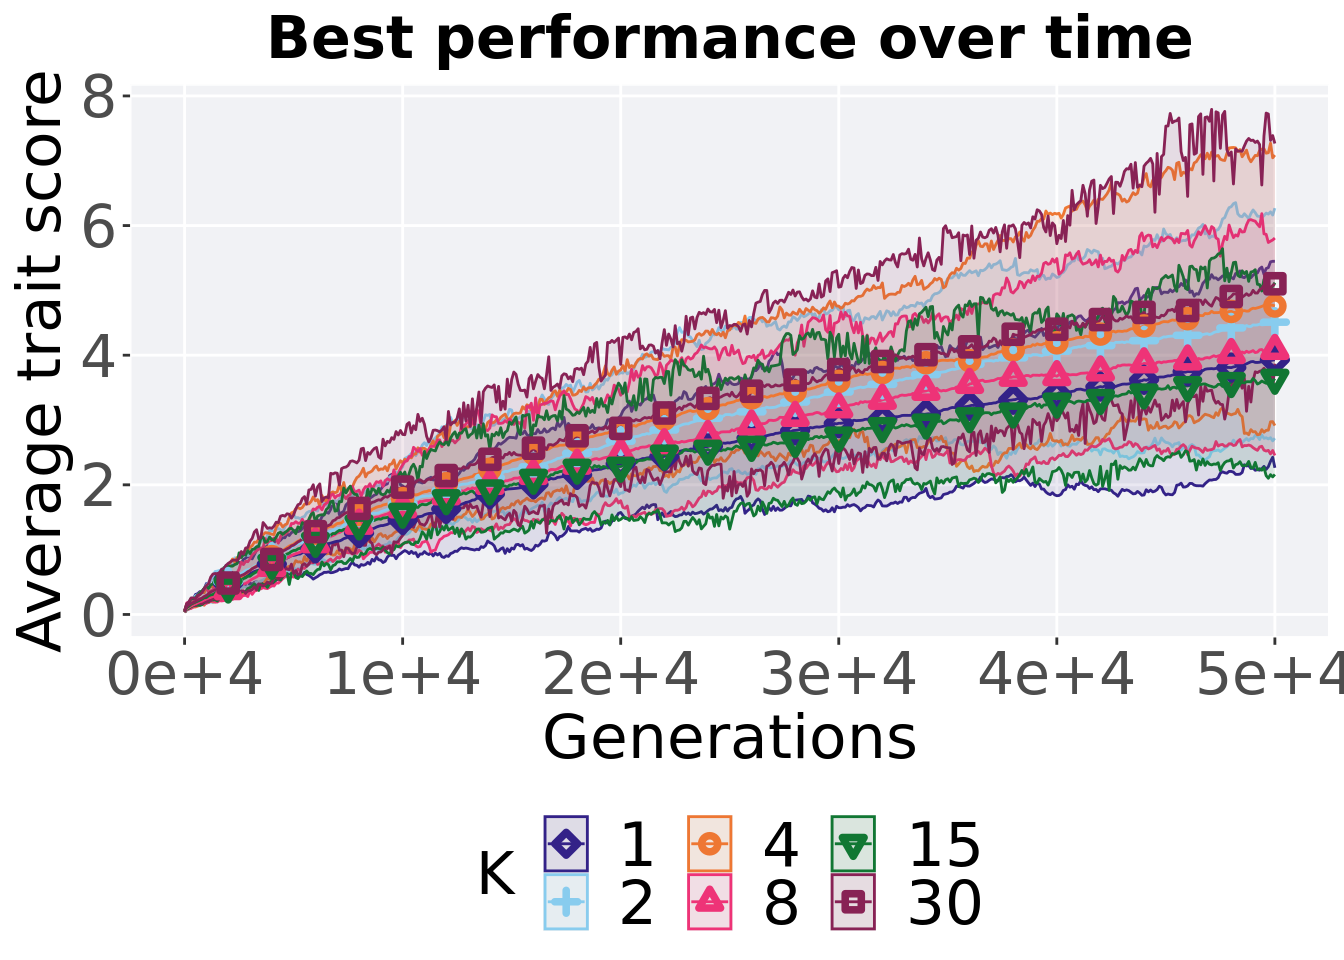
\includegraphics{demo_files/figure-latex/unnamed-chunk-64-1.pdf}

\hypertarget{end-of-50000-generations-4}{%
\subsection{End of 50,000 generations}\label{end-of-50000-generations-4}}

Activation gene coverage in the population at the end of 50,000 generations.

\begin{Shaded}
\begin{Highlighting}[]
\NormalTok{end =}\StringTok{ }\KeywordTok{filter}\NormalTok{(cc_end, diagnostic }\OperatorTok{==}\StringTok{ 'multipath_exploration'}\NormalTok{)}
\NormalTok{end}\OperatorTok{$}\NormalTok{uni_str_pos =}\StringTok{ }\NormalTok{end}\OperatorTok{$}\NormalTok{uni_str_pos }\OperatorTok{+}\StringTok{ }\NormalTok{end}\OperatorTok{$}\NormalTok{arc_acti_gene }\OperatorTok{-}\StringTok{ }\NormalTok{end}\OperatorTok{$}\NormalTok{overlap}
\NormalTok{best =}\StringTok{ }\KeywordTok{ggplot}\NormalTok{(end, }\KeywordTok{aes}\NormalTok{(}\DataTypeTok{x =}\NormalTok{ acron, }\DataTypeTok{y =}\NormalTok{ uni_str_pos, }\DataTypeTok{color =}\NormalTok{ acron, }\DataTypeTok{fill =}\NormalTok{ acron, }\DataTypeTok{shape =}\NormalTok{ acron)) }\OperatorTok{+}
\StringTok{  }\KeywordTok{geom_flat_violin}\NormalTok{(}\DataTypeTok{position =} \KeywordTok{position_nudge}\NormalTok{(}\DataTypeTok{x =} \FloatTok{.2}\NormalTok{, }\DataTypeTok{y =} \DecValTok{0}\NormalTok{), }\DataTypeTok{scale =} \StringTok{'width'}\NormalTok{, }\DataTypeTok{alpha =} \FloatTok{0.2}\NormalTok{) }\OperatorTok{+}
\StringTok{  }\KeywordTok{geom_point}\NormalTok{(}\DataTypeTok{position =} \KeywordTok{position_jitter}\NormalTok{(}\DataTypeTok{width =} \FloatTok{.1}\NormalTok{), }\DataTypeTok{size =} \FloatTok{1.5}\NormalTok{, }\DataTypeTok{alpha =} \FloatTok{1.0}\NormalTok{) }\OperatorTok{+}
\StringTok{  }\KeywordTok{geom_boxplot}\NormalTok{(}\DataTypeTok{color =} \StringTok{'black'}\NormalTok{, }\DataTypeTok{width =} \FloatTok{.2}\NormalTok{, }\DataTypeTok{outlier.shape =} \OtherTok{NA}\NormalTok{, }\DataTypeTok{alpha =} \FloatTok{0.0}\NormalTok{) }\OperatorTok{+}
\StringTok{  }\KeywordTok{scale_y_continuous}\NormalTok{(}
    \DataTypeTok{name=}\StringTok{"Coverage"}\NormalTok{,}
    \DataTypeTok{limits=}\KeywordTok{c}\NormalTok{(}\OperatorTok{-}\DecValTok{1}\NormalTok{, }\DecValTok{101}\NormalTok{),}
    \DataTypeTok{breaks=}\KeywordTok{seq}\NormalTok{(}\DecValTok{0}\NormalTok{,}\DecValTok{100}\NormalTok{, }\DecValTok{20}\NormalTok{),}
    \DataTypeTok{labels=}\KeywordTok{c}\NormalTok{(}\StringTok{"0"}\NormalTok{, }\StringTok{"20"}\NormalTok{, }\StringTok{"40"}\NormalTok{, }\StringTok{"60"}\NormalTok{, }\StringTok{"80"}\NormalTok{, }\StringTok{"100"}\NormalTok{)}
\NormalTok{  ) }\OperatorTok{+}
\StringTok{  }\KeywordTok{scale_x_discrete}\NormalTok{(}
    \DataTypeTok{name=}\StringTok{"Scheme"}
\NormalTok{  )}\OperatorTok{+}
\StringTok{  }\KeywordTok{scale_shape_manual}\NormalTok{(}\DataTypeTok{values=}\NormalTok{SHAPE)}\OperatorTok{+}
\StringTok{  }\KeywordTok{scale_colour_manual}\NormalTok{(}\DataTypeTok{values =}\NormalTok{ cb_palette) }\OperatorTok{+}
\StringTok{  }\KeywordTok{scale_fill_manual}\NormalTok{(}\DataTypeTok{values =}\NormalTok{ cb_palette) }\OperatorTok{+}
\StringTok{  }\NormalTok{p_theme}

\KeywordTok{plot_grid}\NormalTok{(}
\NormalTok{  best }\OperatorTok{+}
\StringTok{    }\KeywordTok{ggtitle}\NormalTok{(}\StringTok{"Final activation gene coverage"}\NormalTok{) }\OperatorTok{+}
\StringTok{    }\KeywordTok{theme}\NormalTok{(}\DataTypeTok{legend.position=}\StringTok{"none"}\NormalTok{),}
\NormalTok{  legend,}
  \DataTypeTok{nrow=}\DecValTok{2}\NormalTok{,}
  \DataTypeTok{rel_heights =} \KeywordTok{c}\NormalTok{(}\DecValTok{2}\NormalTok{,.}\DecValTok{55}\NormalTok{),}
  \DataTypeTok{label_size =}\NormalTok{ TSIZE}
\NormalTok{)}
\end{Highlighting}
\end{Shaded}

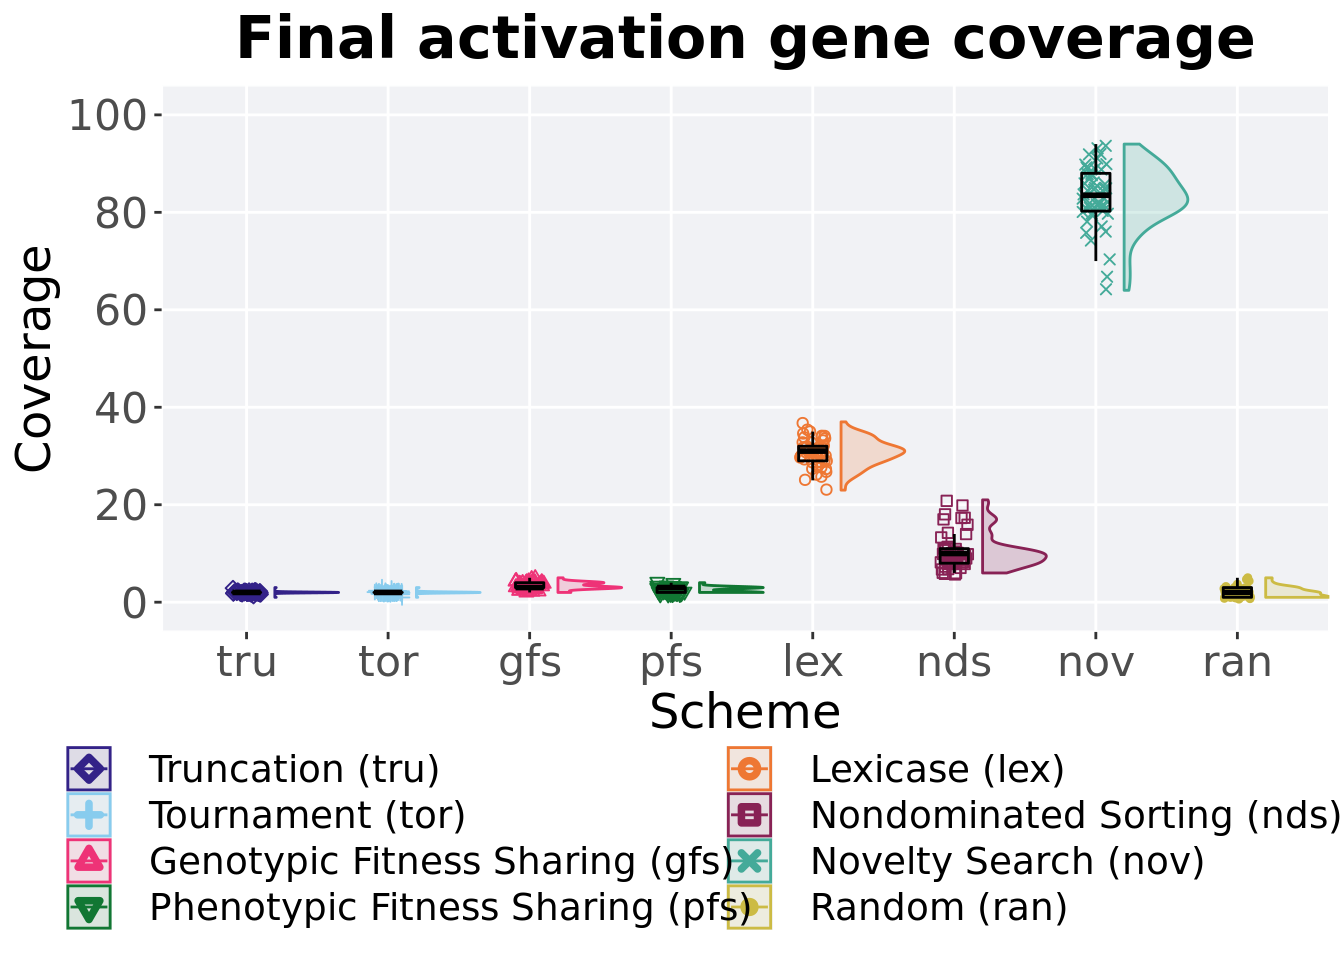
\includegraphics{demo_files/figure-latex/unnamed-chunk-65-1.pdf}

\hypertarget{stats-11}{%
\subsubsection{Stats}\label{stats-11}}

Summary statistics for activation gene coverage in the population at the end of 50,000 generations.

\begin{Shaded}
\begin{Highlighting}[]
\NormalTok{end}\OperatorTok{$}\NormalTok{acron <-}\StringTok{ }\KeywordTok{factor}\NormalTok{(end}\OperatorTok{$}\NormalTok{acron, }\DataTypeTok{levels =} \KeywordTok{c}\NormalTok{(}\StringTok{'nov'}\NormalTok{,}\StringTok{'lex'}\NormalTok{,}\StringTok{'nds'}\NormalTok{,}\StringTok{'gfs'}\NormalTok{,}\StringTok{'pfs'}\NormalTok{,}\StringTok{'ran'}\NormalTok{,}\StringTok{'tor'}\NormalTok{,}\StringTok{'tru'}\NormalTok{))}
\KeywordTok{group_by}\NormalTok{(end, acron) }\OperatorTok
\StringTok{  }\NormalTok{dplyr}\OperatorTok{::}\KeywordTok{summarise}\NormalTok{(}
    \DataTypeTok{count =} \KeywordTok{n}\NormalTok{(),}
    \DataTypeTok{na_cnt =} \KeywordTok{sum}\NormalTok{(}\KeywordTok{is.na}\NormalTok{(uni_str_pos)),}
    \DataTypeTok{min =} \KeywordTok{min}\NormalTok{(uni_str_pos, }\DataTypeTok{na.rm =} \OtherTok{TRUE}\NormalTok{),}
    \DataTypeTok{median =} \KeywordTok{median}\NormalTok{(uni_str_pos, }\DataTypeTok{na.rm =} \OtherTok{TRUE}\NormalTok{),}
    \DataTypeTok{mean =} \KeywordTok{mean}\NormalTok{(uni_str_pos, }\DataTypeTok{na.rm =} \OtherTok{TRUE}\NormalTok{),}
    \DataTypeTok{max =} \KeywordTok{max}\NormalTok{(uni_str_pos, }\DataTypeTok{na.rm =} \OtherTok{TRUE}\NormalTok{),}
    \DataTypeTok{IQR =} \KeywordTok{IQR}\NormalTok{(uni_str_pos, }\DataTypeTok{na.rm =} \OtherTok{TRUE}\NormalTok{)}
\NormalTok{  )}
\end{Highlighting}
\end{Shaded}

\begin{verbatim}
## # A tibble: 8 x 8
##   acron count na_cnt   min median  mean   max   IQR
##   <fct> <int>  <int> <int>  <dbl> <dbl> <int> <dbl>
## 1 nov      50      0    64   83.5 83.2     94  7.75
## 2 lex      50      0    23   31   30.7     37  3   
## 3 nds      50      0     6   10   10.4     21  3   
## 4 gfs      50      0     2    3    3.34     5  1   
## 5 pfs      50      0     2    3    2.56     4  1   
## 6 ran      50      0     1    2    2        5  2   
## 7 tor      50      0     1    2    2.02     3  0   
## 8 tru      50      0     1    2    2        3  0
\end{verbatim}

Kruskal--Wallis test provides evidence of difference among activation gene coverage in the population at the end of 50,000 generations.

\begin{Shaded}
\begin{Highlighting}[]
\KeywordTok{kruskal.test}\NormalTok{(uni_str_pos }\OperatorTok{~}\StringTok{ }\NormalTok{acron,}\DataTypeTok{data =}\NormalTok{ end)}
\end{Highlighting}
\end{Shaded}

\begin{verbatim}
## 
##  Kruskal-Wallis rank sum test
## 
## data:  uni_str_pos by acron
## Kruskal-Wallis chi-squared = 350.16, df = 7, p-value < 2.2e-16
\end{verbatim}

Results for post-hoc Wilcoxon rank-sum test with a Bonferroni correction on activation gene coverage in the population at the end of 50,000 generations.

\begin{Shaded}
\begin{Highlighting}[]
\KeywordTok{pairwise.wilcox.test}\NormalTok{(}\DataTypeTok{x =}\NormalTok{ end}\OperatorTok{$}\NormalTok{uni_str_pos, }\DataTypeTok{g =}\NormalTok{ end}\OperatorTok{$}\NormalTok{acron, }\DataTypeTok{p.adjust.method =} \StringTok{"bonferroni"}\NormalTok{,}
                     \DataTypeTok{paired =} \OtherTok{FALSE}\NormalTok{, }\DataTypeTok{conf.int =} \OtherTok{FALSE}\NormalTok{, }\DataTypeTok{alternative =} \StringTok{'l'}\NormalTok{)}
\end{Highlighting}
\end{Shaded}

\begin{verbatim}
## 
##  Pairwise comparisons using Wilcoxon rank sum test with continuity correction 
## 
## data:  end$uni_str_pos and end$acron 
## 
##     nov     lex     nds     gfs     pfs     ran    tor   
## lex < 2e-16 -       -       -       -       -      -     
## nds < 2e-16 < 2e-16 -       -       -       -      -     
## gfs < 2e-16 < 2e-16 < 2e-16 -       -       -      -     
## pfs < 2e-16 < 2e-16 < 2e-16 3.3e-06 -       -      -     
## ran < 2e-16 < 2e-16 < 2e-16 1.2e-08 0.0036  -      -     
## tor < 2e-16 < 2e-16 < 2e-16 1.7e-15 1.2e-06 1.0000 -     
## tru < 2e-16 < 2e-16 < 2e-16 5.0e-16 2.6e-07 1.0000 1.0000
## 
## P value adjustment method: bonferroni
\end{verbatim}

\hypertarget{truncation-selection}{%
\chapter{Truncation selection}\label{truncation-selection}}

We present the results from our parameter sweeep on truncation selection.
50 replicates are conducted for each truncation size \texttt{T} parameter value explored.

\begin{Shaded}
\begin{Highlighting}[]
\KeywordTok{library}\NormalTok{(ggplot2)}
\KeywordTok{library}\NormalTok{(cowplot)}
\KeywordTok{library}\NormalTok{(dplyr)}
\KeywordTok{library}\NormalTok{(PupillometryR)}
\end{Highlighting}
\end{Shaded}

These analyses were conducted in the following computing environment:

\begin{Shaded}
\begin{Highlighting}[]
\KeywordTok{print}\NormalTok{(version)}
\end{Highlighting}
\end{Shaded}

\begin{verbatim}
##                _                           
## platform       x86_64-pc-linux-gnu         
## arch           x86_64                      
## os             linux-gnu                   
## system         x86_64, linux-gnu           
## status                                     
## major          4                           
## minor          2.1                         
## year           2022                        
## month          06                          
## day            23                          
## svn rev        82513                       
## language       R                           
## version.string R version 4.2.1 (2022-06-23)
## nickname       Funny-Looking Kid
\end{verbatim}

\hypertarget{exploitation-rate-results-1}{%
\section{Exploitation rate results}\label{exploitation-rate-results-1}}

Here we present the results for \textbf{best performances} found by each genotypic fitness sharing sigma value replicate on the exploitation rate diagnostic.
Best performance found refers to the largest average trait score found in a given population.
Note that performance values fall between 0 and 100.

\hypertarget{performance-over-time-2}{%
\subsection{Performance over time}\label{performance-over-time-2}}

Performance over time.

\begin{Shaded}
\begin{Highlighting}[]
\NormalTok{problem <-}\StringTok{ }\KeywordTok{filter}\NormalTok{(tru_ot, diagnostic }\OperatorTok{==}\StringTok{ 'exploitation_rate'}\NormalTok{)}
\NormalTok{lines =}\StringTok{ }\NormalTok{problem }\OperatorTok
\StringTok{        }\KeywordTok{group_by}\NormalTok{(T, gen) }\OperatorTok
\StringTok{          }\NormalTok{dplyr}\OperatorTok{::}\KeywordTok{summarise}\NormalTok{(}
            \DataTypeTok{min =} \KeywordTok{min}\NormalTok{(pop_fit_max),}
            \DataTypeTok{mean =} \KeywordTok{mean}\NormalTok{(pop_fit_max),}
            \DataTypeTok{max =} \KeywordTok{max}\NormalTok{(pop_fit_max)}
\NormalTok{          )}
\end{Highlighting}
\end{Shaded}

\begin{verbatim}
## `summarise()` has grouped output by 'T'. You can override using the `.groups`
## argument.
\end{verbatim}

\begin{Shaded}
\begin{Highlighting}[]
\NormalTok{points =}\StringTok{ }\KeywordTok{filter}\NormalTok{(lines, gen }\OperatorTok\StringTok{ }\DecValTok{2000} \OperatorTok{==}\StringTok{ }\DecValTok{0} \OperatorTok{&}\StringTok{ }\NormalTok{gen }\OperatorTok{!=}\StringTok{ }\DecValTok{0}\NormalTok{)}

\NormalTok{ot =}\StringTok{ }\KeywordTok{ggplot}\NormalTok{(lines, }\KeywordTok{aes}\NormalTok{(}\DataTypeTok{x=}\NormalTok{gen, }\DataTypeTok{y=}\NormalTok{mean }\OperatorTok{/}\StringTok{ }\NormalTok{TRAITS, }\DataTypeTok{group =}\NormalTok{ T, }\DataTypeTok{fill =}\NormalTok{ T, }\DataTypeTok{color =}\NormalTok{ T, }\DataTypeTok{shape =}\NormalTok{ T)) }\OperatorTok{+}
\StringTok{  }\KeywordTok{geom_ribbon}\NormalTok{(}\KeywordTok{aes}\NormalTok{(}\DataTypeTok{ymin =}\NormalTok{ min }\OperatorTok{/}\StringTok{ }\NormalTok{TRAITS, }\DataTypeTok{ymax =}\NormalTok{ max }\OperatorTok{/}\StringTok{ }\NormalTok{TRAITS), }\DataTypeTok{alpha =} \FloatTok{0.1}\NormalTok{) }\OperatorTok{+}
\StringTok{  }\KeywordTok{geom_line}\NormalTok{(}\DataTypeTok{size =} \FloatTok{0.5}\NormalTok{) }\OperatorTok{+}
\StringTok{  }\KeywordTok{geom_point}\NormalTok{(}\DataTypeTok{data =}\NormalTok{ points, }\DataTypeTok{size =} \FloatTok{1.5}\NormalTok{, }\DataTypeTok{stroke =} \FloatTok{2.0}\NormalTok{, }\DataTypeTok{alpha =} \FloatTok{1.0}\NormalTok{) }\OperatorTok{+}
\StringTok{  }\KeywordTok{scale_y_continuous}\NormalTok{(}
    \DataTypeTok{name=}\StringTok{"Average trait score"}\NormalTok{,}
    \DataTypeTok{limits=}\KeywordTok{c}\NormalTok{(}\OperatorTok{-}\DecValTok{1}\NormalTok{, }\DecValTok{101}\NormalTok{),}
    \DataTypeTok{breaks=}\KeywordTok{seq}\NormalTok{(}\DecValTok{0}\NormalTok{,}\DecValTok{100}\NormalTok{, }\DecValTok{20}\NormalTok{),}
    \DataTypeTok{labels=}\KeywordTok{c}\NormalTok{(}\StringTok{"0"}\NormalTok{, }\StringTok{"20"}\NormalTok{, }\StringTok{"40"}\NormalTok{, }\StringTok{"60"}\NormalTok{, }\StringTok{"80"}\NormalTok{, }\StringTok{"100"}\NormalTok{)}
\NormalTok{  ) }\OperatorTok{+}
\StringTok{  }\KeywordTok{scale_x_continuous}\NormalTok{(}
    \DataTypeTok{name=}\StringTok{"Generations"}\NormalTok{,}
    \DataTypeTok{limits=}\KeywordTok{c}\NormalTok{(}\DecValTok{0}\NormalTok{, }\DecValTok{50000}\NormalTok{),}
    \DataTypeTok{breaks=}\KeywordTok{c}\NormalTok{(}\DecValTok{0}\NormalTok{, }\DecValTok{10000}\NormalTok{, }\DecValTok{20000}\NormalTok{, }\DecValTok{30000}\NormalTok{, }\DecValTok{40000}\NormalTok{, }\DecValTok{50000}\NormalTok{),}
    \DataTypeTok{labels=}\KeywordTok{c}\NormalTok{(}\StringTok{"0e+6"}\NormalTok{, }\StringTok{"1e+6"}\NormalTok{, }\StringTok{"2e+6"}\NormalTok{, }\StringTok{"3e+6"}\NormalTok{, }\StringTok{"4e+6"}\NormalTok{, }\StringTok{"5e+6"}\NormalTok{)}

\NormalTok{  ) }\OperatorTok{+}
\StringTok{  }\KeywordTok{scale_shape_manual}\NormalTok{(}\DataTypeTok{values=}\NormalTok{SHAPE)}\OperatorTok{+}
\StringTok{  }\KeywordTok{scale_colour_manual}\NormalTok{(}\DataTypeTok{values =}\NormalTok{ cb_palette) }\OperatorTok{+}
\StringTok{  }\KeywordTok{scale_fill_manual}\NormalTok{(}\DataTypeTok{values =}\NormalTok{ cb_palette) }\OperatorTok{+}
\StringTok{  }\KeywordTok{ggtitle}\NormalTok{(}\StringTok{"Best performance over time"}\NormalTok{) }\OperatorTok{+}
\StringTok{  }\NormalTok{p_theme}\OperatorTok{+}
\StringTok{    }\KeywordTok{guides}\NormalTok{(}
    \DataTypeTok{shape=}\KeywordTok{guide_legend}\NormalTok{(}\DataTypeTok{nrow=}\DecValTok{1}\NormalTok{, }\DataTypeTok{title.position =} \StringTok{"bottom"}\NormalTok{),}
    \DataTypeTok{color=}\KeywordTok{guide_legend}\NormalTok{(}\DataTypeTok{nrow=}\DecValTok{1}\NormalTok{, }\DataTypeTok{title.position =} \StringTok{"bottom"}\NormalTok{),}
    \DataTypeTok{fill=}\KeywordTok{guide_legend}\NormalTok{(}\DataTypeTok{nrow=}\DecValTok{1}\NormalTok{, }\DataTypeTok{title.position =} \StringTok{"bottom"}\NormalTok{)}
\NormalTok{  ) }\OperatorTok{+}
\StringTok{  }\KeywordTok{theme}\NormalTok{(}
    \DataTypeTok{legend.position =} \StringTok{"bottom"}\NormalTok{,}
    \DataTypeTok{legend.box=}\StringTok{"verticle"}\NormalTok{,}
    \DataTypeTok{legend.justification=}\StringTok{"center"}\NormalTok{,}
    \DataTypeTok{legend.title.align=}\FloatTok{0.5}
\NormalTok{  )}

\NormalTok{ot}
\end{Highlighting}
\end{Shaded}

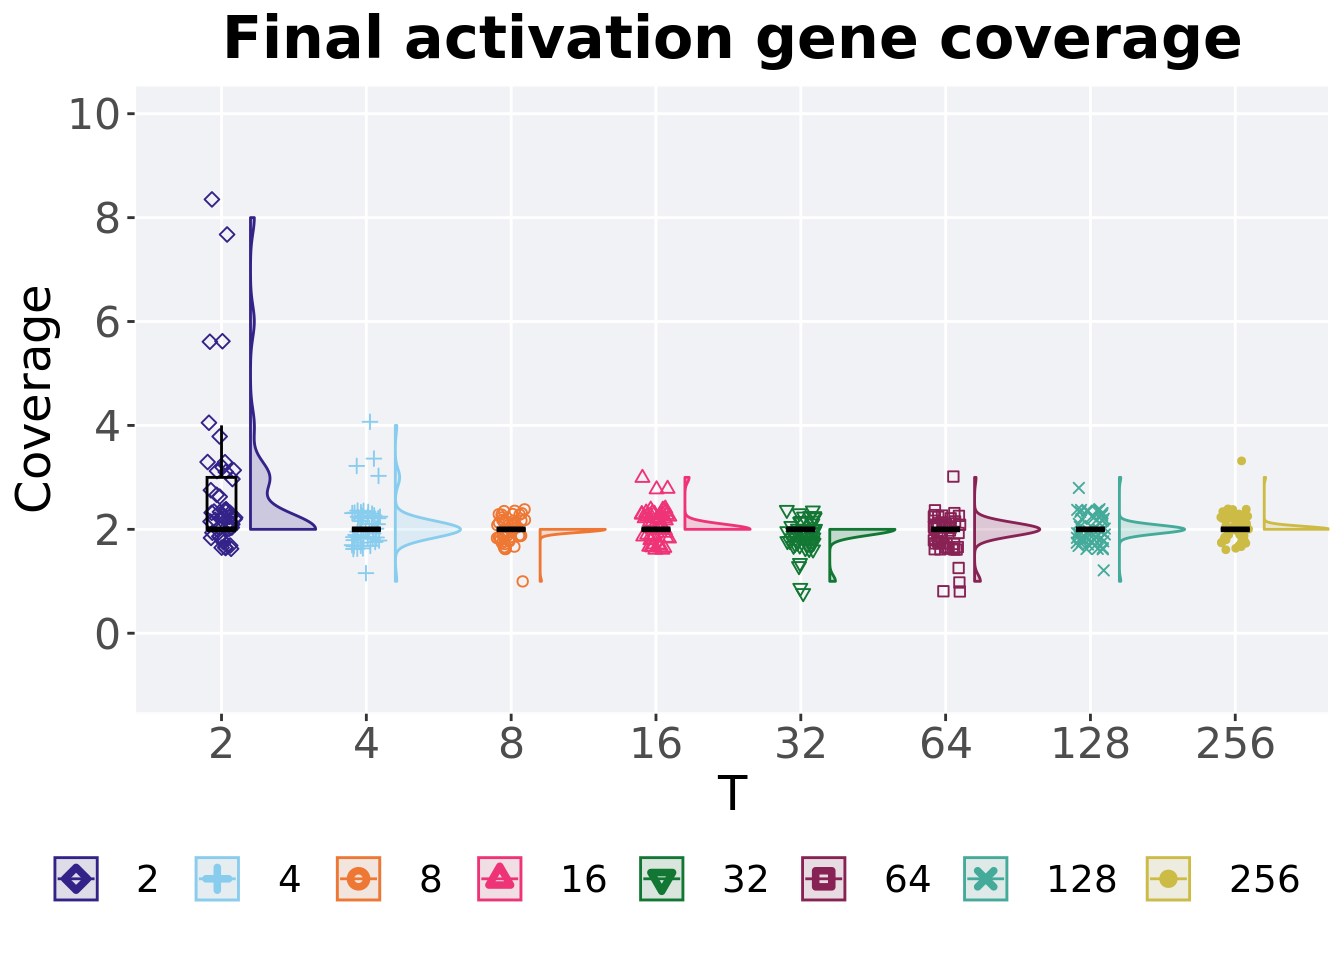
\includegraphics{demo_files/figure-latex/unnamed-chunk-71-1.pdf}

\hypertarget{generation-satisfactory-solution-found-2}{%
\subsection{Generation satisfactory solution found}\label{generation-satisfactory-solution-found-2}}

The first generation a satisfactory solution is found throughout the 50,000 generations.

\begin{Shaded}
\begin{Highlighting}[]
\NormalTok{ssf =}\StringTok{ }\KeywordTok{filter}\NormalTok{(tru_ssf, diagnostic }\OperatorTok{==}\StringTok{ 'exploitation_rate'}\NormalTok{)}

\NormalTok{plot <-}\StringTok{ }\KeywordTok{ggplot}\NormalTok{(ssf, }\KeywordTok{aes}\NormalTok{(}\DataTypeTok{x =}\NormalTok{ T, }\DataTypeTok{y =}\NormalTok{ generation, }\DataTypeTok{color =}\NormalTok{ T, }\DataTypeTok{fill =}\NormalTok{ T, }\DataTypeTok{shape =}\NormalTok{ T)) }\OperatorTok{+}
\StringTok{  }\KeywordTok{geom_flat_violin}\NormalTok{(}\DataTypeTok{position =} \KeywordTok{position_nudge}\NormalTok{(}\DataTypeTok{x =} \FloatTok{.2}\NormalTok{, }\DataTypeTok{y =} \DecValTok{0}\NormalTok{), }\DataTypeTok{scale =} \StringTok{'width'}\NormalTok{, }\DataTypeTok{alpha =} \FloatTok{0.2}\NormalTok{) }\OperatorTok{+}
\StringTok{  }\KeywordTok{geom_point}\NormalTok{(}\DataTypeTok{position =} \KeywordTok{position_jitter}\NormalTok{(}\DataTypeTok{width =} \FloatTok{.1}\NormalTok{), }\DataTypeTok{size =} \FloatTok{1.5}\NormalTok{, }\DataTypeTok{alpha =} \FloatTok{1.0}\NormalTok{) }\OperatorTok{+}
\StringTok{  }\KeywordTok{geom_boxplot}\NormalTok{(}\DataTypeTok{color =} \StringTok{'black'}\NormalTok{, }\DataTypeTok{width =} \FloatTok{.2}\NormalTok{, }\DataTypeTok{outlier.shape =} \OtherTok{NA}\NormalTok{, }\DataTypeTok{alpha =} \FloatTok{0.0}\NormalTok{) }\OperatorTok{+}
\StringTok{  }\KeywordTok{scale_shape_manual}\NormalTok{(}\DataTypeTok{values=}\NormalTok{SHAPE)}\OperatorTok{+}
\StringTok{  }\KeywordTok{scale_y_continuous}\NormalTok{(}
    \DataTypeTok{name=}\StringTok{"Generation"}\NormalTok{,}
    \DataTypeTok{limits=}\KeywordTok{c}\NormalTok{(}\DecValTok{0}\NormalTok{, }\DecValTok{12000}\NormalTok{),}
    \DataTypeTok{breaks=}\KeywordTok{c}\NormalTok{(}\DecValTok{0}\NormalTok{, }\DecValTok{2000}\NormalTok{, }\DecValTok{4000}\NormalTok{, }\DecValTok{6000}\NormalTok{, }\DecValTok{8000}\NormalTok{, }\DecValTok{10000}\NormalTok{, }\DecValTok{12000}\NormalTok{),}
    \DataTypeTok{labels=}\KeywordTok{c}\NormalTok{(}\StringTok{"0e+6"}\NormalTok{, }\StringTok{"2e+6"}\NormalTok{, }\StringTok{"4e+6"}\NormalTok{, }\StringTok{"6e+6"}\NormalTok{, }\StringTok{"8e+6"}\NormalTok{, }\StringTok{"10e+6"}\NormalTok{, }\StringTok{"12e+6"}\NormalTok{)}
\NormalTok{  ) }\OperatorTok{+}
\StringTok{  }\KeywordTok{scale_x_discrete}\NormalTok{(}
    \DataTypeTok{name=}\StringTok{"T"}
\NormalTok{  ) }\OperatorTok{+}
\StringTok{  }\KeywordTok{scale_colour_manual}\NormalTok{(}\DataTypeTok{values =}\NormalTok{ cb_palette) }\OperatorTok{+}
\StringTok{  }\KeywordTok{scale_fill_manual}\NormalTok{(}\DataTypeTok{values =}\NormalTok{ cb_palette) }\OperatorTok{+}
\StringTok{  }\NormalTok{p_theme}

\KeywordTok{plot_grid}\NormalTok{(}
\NormalTok{  plot }\OperatorTok{+}
\StringTok{    }\KeywordTok{ggtitle}\NormalTok{(}\StringTok{"Generation satisfactory solution found"}\NormalTok{) }\OperatorTok{+}
\StringTok{    }\KeywordTok{theme}\NormalTok{(}\DataTypeTok{legend.position=}\StringTok{"none"}\NormalTok{),}
\NormalTok{  legend,}
  \DataTypeTok{nrow=}\DecValTok{2}\NormalTok{,}
  \DataTypeTok{rel_heights =} \KeywordTok{c}\NormalTok{(}\DecValTok{2}\NormalTok{,.}\DecValTok{2}\NormalTok{),}
  \DataTypeTok{label_size =}\NormalTok{ TSIZE}
\NormalTok{)}
\end{Highlighting}
\end{Shaded}

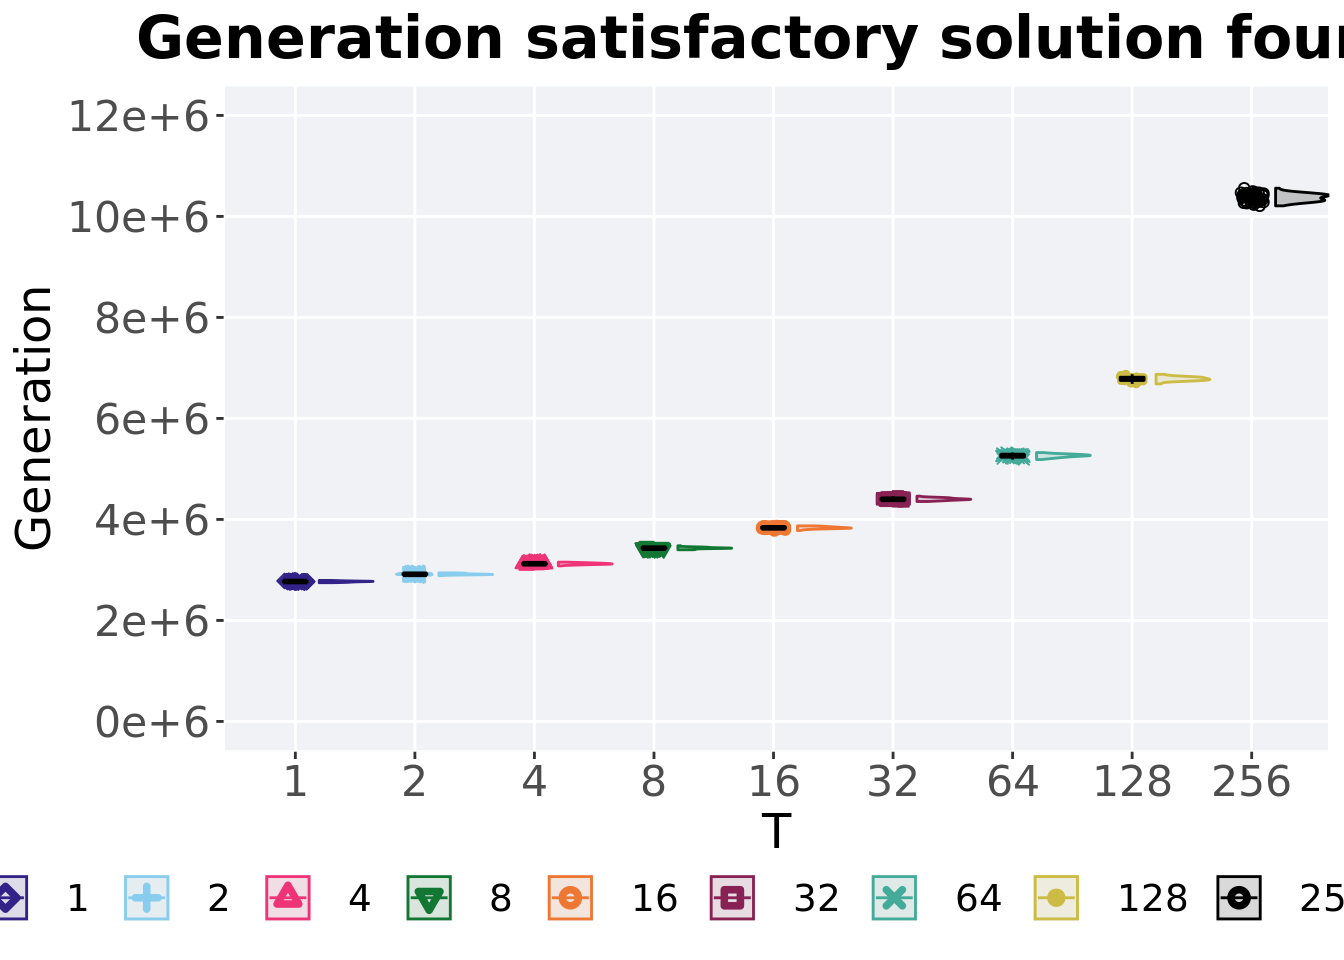
\includegraphics{demo_files/figure-latex/unnamed-chunk-73-1.pdf}

\hypertarget{stats-12}{%
\subsubsection{Stats}\label{stats-12}}

Summary statistics for the first generation a satisfactory solution is found throughout the 50,000 generations.

\begin{Shaded}
\begin{Highlighting}[]
\KeywordTok{group_by}\NormalTok{(ssf, T) }\OperatorTok
\StringTok{  }\NormalTok{dplyr}\OperatorTok{::}\KeywordTok{summarise}\NormalTok{(}
    \DataTypeTok{count =} \KeywordTok{n}\NormalTok{(),}
    \DataTypeTok{na_cnt =} \KeywordTok{sum}\NormalTok{(}\KeywordTok{is.na}\NormalTok{(generation)),}
    \DataTypeTok{min =} \KeywordTok{min}\NormalTok{(generation, }\DataTypeTok{na.rm =} \OtherTok{TRUE}\NormalTok{),}
    \DataTypeTok{median =} \KeywordTok{median}\NormalTok{(generation, }\DataTypeTok{na.rm =} \OtherTok{TRUE}\NormalTok{),}
    \DataTypeTok{mean =} \KeywordTok{mean}\NormalTok{(generation, }\DataTypeTok{na.rm =} \OtherTok{TRUE}\NormalTok{),}
    \DataTypeTok{max =} \KeywordTok{max}\NormalTok{(generation, }\DataTypeTok{na.rm =} \OtherTok{TRUE}\NormalTok{),}
    \DataTypeTok{IQR =} \KeywordTok{IQR}\NormalTok{(generation, }\DataTypeTok{na.rm =} \OtherTok{TRUE}\NormalTok{)}
\NormalTok{  )}
\end{Highlighting}
\end{Shaded}

\begin{verbatim}
## # A tibble: 9 x 8
##   T     count na_cnt   min median   mean   max   IQR
##   <fct> <int>  <int> <dbl>  <dbl>  <dbl> <dbl> <dbl>
## 1 1        50      0  2746  2771   2769.  2792  15.5
## 2 2        50      0  2886  2914.  2917.  2941  19.8
## 3 4        50      0  3080  3122.  3121.  3154  19.8
## 4 8        50      0  3399  3430.  3432.  3478  18  
## 5 16       50      0  3779  3833   3835.  3872  26.8
## 6 32       50      0  4355  4398.  4401.  4460  33.2
## 7 64       50      0  5185  5264   5261.  5324  44.5
## 8 128      50      0  6684  6784   6785.  6874  60.2
## 9 256      50      0 10209 10369  10371. 10559 109.
\end{verbatim}

Kruskal--Wallis test provides evidence of significant differences among the generation a satisfactory solution is first found.

\begin{Shaded}
\begin{Highlighting}[]
\KeywordTok{kruskal.test}\NormalTok{(generation }\OperatorTok{~}\StringTok{ }\NormalTok{T,}\DataTypeTok{data =}\NormalTok{ ssf)}
\end{Highlighting}
\end{Shaded}

\begin{verbatim}
## 
##  Kruskal-Wallis rank sum test
## 
## data:  generation by T
## Kruskal-Wallis chi-squared = 443.46, df = 8, p-value < 2.2e-16
\end{verbatim}

Results for post-hoc Wilcoxon rank-sum test with a Bonferroni correction on the generation a satisfactory solution is first found. .

\begin{Shaded}
\begin{Highlighting}[]
\KeywordTok{pairwise.wilcox.test}\NormalTok{(}\DataTypeTok{x =}\NormalTok{ ssf}\OperatorTok{$}\NormalTok{generation, }\DataTypeTok{g =}\NormalTok{ ssf}\OperatorTok{$}\NormalTok{T , }\DataTypeTok{p.adjust.method =} \StringTok{"bonferroni"}\NormalTok{,}
                     \DataTypeTok{paired =} \OtherTok{FALSE}\NormalTok{, }\DataTypeTok{conf.int =} \OtherTok{FALSE}\NormalTok{, }\DataTypeTok{alternative =} \StringTok{'g'}\NormalTok{)}
\end{Highlighting}
\end{Shaded}

\begin{verbatim}
## 
##  Pairwise comparisons using Wilcoxon rank sum test with continuity correction 
## 
## data:  ssf$generation and ssf$T 
## 
##     1      2      4      8      16     32     64     128   
## 2   <2e-16 -      -      -      -      -      -      -     
## 4   <2e-16 <2e-16 -      -      -      -      -      -     
## 8   <2e-16 <2e-16 <2e-16 -      -      -      -      -     
## 16  <2e-16 <2e-16 <2e-16 <2e-16 -      -      -      -     
## 32  <2e-16 <2e-16 <2e-16 <2e-16 <2e-16 -      -      -     
## 64  <2e-16 <2e-16 <2e-16 <2e-16 <2e-16 <2e-16 -      -     
## 128 <2e-16 <2e-16 <2e-16 <2e-16 <2e-16 <2e-16 <2e-16 -     
## 256 <2e-16 <2e-16 <2e-16 <2e-16 <2e-16 <2e-16 <2e-16 <2e-16
## 
## P value adjustment method: bonferroni
\end{verbatim}

\hypertarget{ordered-exploitation-results-1}{%
\section{Ordered exploitation results}\label{ordered-exploitation-results-1}}

Here we present the results for \textbf{best performances} found by each genotypic fitness sharing sigma value replicate on the ordered exploitation diagnostic.
Best performance found refers to the largest average trait score found in a given population.
Note that performance values fall between 0 and 100.

\hypertarget{performance-over-time-3}{%
\subsection{Performance over time}\label{performance-over-time-3}}

Performance over time.

\begin{Shaded}
\begin{Highlighting}[]
\NormalTok{problem <-}\StringTok{ }\KeywordTok{filter}\NormalTok{(tru_ot, diagnostic }\OperatorTok{==}\StringTok{ 'ordered_exploitation'}\NormalTok{)}
\NormalTok{lines =}\StringTok{ }\NormalTok{problem }\OperatorTok
\StringTok{        }\KeywordTok{group_by}\NormalTok{(T, gen) }\OperatorTok
\StringTok{          }\NormalTok{dplyr}\OperatorTok{::}\KeywordTok{summarise}\NormalTok{(}
            \DataTypeTok{min =} \KeywordTok{min}\NormalTok{(pop_fit_max),}
            \DataTypeTok{mean =} \KeywordTok{mean}\NormalTok{(pop_fit_max),}
            \DataTypeTok{max =} \KeywordTok{max}\NormalTok{(pop_fit_max)}
\NormalTok{          )}
\end{Highlighting}
\end{Shaded}

\begin{verbatim}
## `summarise()` has grouped output by 'T'. You can override using the `.groups`
## argument.
\end{verbatim}

\begin{Shaded}
\begin{Highlighting}[]
\NormalTok{points =}\StringTok{ }\KeywordTok{filter}\NormalTok{(lines, gen }\OperatorTok\StringTok{ }\DecValTok{2000} \OperatorTok{==}\StringTok{ }\DecValTok{0} \OperatorTok{&}\StringTok{ }\NormalTok{gen }\OperatorTok{!=}\StringTok{ }\DecValTok{0}\NormalTok{)}

\NormalTok{ot =}\StringTok{ }\KeywordTok{ggplot}\NormalTok{(lines, }\KeywordTok{aes}\NormalTok{(}\DataTypeTok{x=}\NormalTok{gen, }\DataTypeTok{y=}\NormalTok{mean }\OperatorTok{/}\StringTok{ }\NormalTok{TRAITS, }\DataTypeTok{group =}\NormalTok{ T, }\DataTypeTok{fill =}\NormalTok{ T, }\DataTypeTok{color =}\NormalTok{ T, }\DataTypeTok{shape =}\NormalTok{ T)) }\OperatorTok{+}
\StringTok{  }\KeywordTok{geom_ribbon}\NormalTok{(}\KeywordTok{aes}\NormalTok{(}\DataTypeTok{ymin =}\NormalTok{ min }\OperatorTok{/}\StringTok{ }\NormalTok{TRAITS, }\DataTypeTok{ymax =}\NormalTok{ max }\OperatorTok{/}\StringTok{ }\NormalTok{TRAITS), }\DataTypeTok{alpha =} \FloatTok{0.1}\NormalTok{) }\OperatorTok{+}
\StringTok{  }\KeywordTok{geom_line}\NormalTok{(}\DataTypeTok{size =} \FloatTok{0.5}\NormalTok{) }\OperatorTok{+}
\StringTok{  }\KeywordTok{geom_point}\NormalTok{(}\DataTypeTok{data =}\NormalTok{ points, }\DataTypeTok{size =} \FloatTok{1.5}\NormalTok{, }\DataTypeTok{stroke =} \FloatTok{2.0}\NormalTok{, }\DataTypeTok{alpha =} \FloatTok{1.0}\NormalTok{) }\OperatorTok{+}
\StringTok{  }\KeywordTok{scale_y_continuous}\NormalTok{(}
    \DataTypeTok{name=}\StringTok{"Average trait score"}\NormalTok{,}
    \DataTypeTok{limits=}\KeywordTok{c}\NormalTok{(}\OperatorTok{-}\DecValTok{1}\NormalTok{, }\DecValTok{101}\NormalTok{),}
    \DataTypeTok{breaks=}\KeywordTok{seq}\NormalTok{(}\DecValTok{0}\NormalTok{,}\DecValTok{100}\NormalTok{, }\DecValTok{20}\NormalTok{),}
    \DataTypeTok{labels=}\KeywordTok{c}\NormalTok{(}\StringTok{"0"}\NormalTok{, }\StringTok{"20"}\NormalTok{, }\StringTok{"40"}\NormalTok{, }\StringTok{"60"}\NormalTok{, }\StringTok{"80"}\NormalTok{, }\StringTok{"100"}\NormalTok{)}
\NormalTok{  ) }\OperatorTok{+}
\StringTok{  }\KeywordTok{scale_x_continuous}\NormalTok{(}
    \DataTypeTok{name=}\StringTok{"Generations"}\NormalTok{,}
    \DataTypeTok{limits=}\KeywordTok{c}\NormalTok{(}\DecValTok{0}\NormalTok{, }\DecValTok{50000}\NormalTok{),}
    \DataTypeTok{breaks=}\KeywordTok{c}\NormalTok{(}\DecValTok{0}\NormalTok{, }\DecValTok{10000}\NormalTok{, }\DecValTok{20000}\NormalTok{, }\DecValTok{30000}\NormalTok{, }\DecValTok{40000}\NormalTok{, }\DecValTok{50000}\NormalTok{),}
    \DataTypeTok{labels=}\KeywordTok{c}\NormalTok{(}\StringTok{"0e+6"}\NormalTok{, }\StringTok{"1e+6"}\NormalTok{, }\StringTok{"2e+6"}\NormalTok{, }\StringTok{"3e+6"}\NormalTok{, }\StringTok{"4e+6"}\NormalTok{, }\StringTok{"5e+6"}\NormalTok{)}

\NormalTok{  ) }\OperatorTok{+}
\StringTok{  }\KeywordTok{scale_shape_manual}\NormalTok{(}\DataTypeTok{values=}\NormalTok{SHAPE)}\OperatorTok{+}
\StringTok{  }\KeywordTok{scale_colour_manual}\NormalTok{(}\DataTypeTok{values =}\NormalTok{ cb_palette) }\OperatorTok{+}
\StringTok{  }\KeywordTok{scale_fill_manual}\NormalTok{(}\DataTypeTok{values =}\NormalTok{ cb_palette) }\OperatorTok{+}
\StringTok{  }\KeywordTok{ggtitle}\NormalTok{(}\StringTok{"Best performance over time"}\NormalTok{) }\OperatorTok{+}
\StringTok{  }\NormalTok{p_theme}\OperatorTok{+}
\StringTok{    }\KeywordTok{guides}\NormalTok{(}
    \DataTypeTok{shape=}\KeywordTok{guide_legend}\NormalTok{(}\DataTypeTok{nrow=}\DecValTok{1}\NormalTok{, }\DataTypeTok{title.position =} \StringTok{"bottom"}\NormalTok{),}
    \DataTypeTok{color=}\KeywordTok{guide_legend}\NormalTok{(}\DataTypeTok{nrow=}\DecValTok{1}\NormalTok{, }\DataTypeTok{title.position =} \StringTok{"bottom"}\NormalTok{),}
    \DataTypeTok{fill=}\KeywordTok{guide_legend}\NormalTok{(}\DataTypeTok{nrow=}\DecValTok{1}\NormalTok{, }\DataTypeTok{title.position =} \StringTok{"bottom"}\NormalTok{)}
\NormalTok{  ) }\OperatorTok{+}
\StringTok{  }\KeywordTok{theme}\NormalTok{(}
    \DataTypeTok{legend.position =} \StringTok{"bottom"}\NormalTok{,}
    \DataTypeTok{legend.box=}\StringTok{"verticle"}\NormalTok{,}
    \DataTypeTok{legend.justification=}\StringTok{"center"}\NormalTok{,}
    \DataTypeTok{legend.title.align=}\FloatTok{0.5}
\NormalTok{  )}

\NormalTok{ot}
\end{Highlighting}
\end{Shaded}

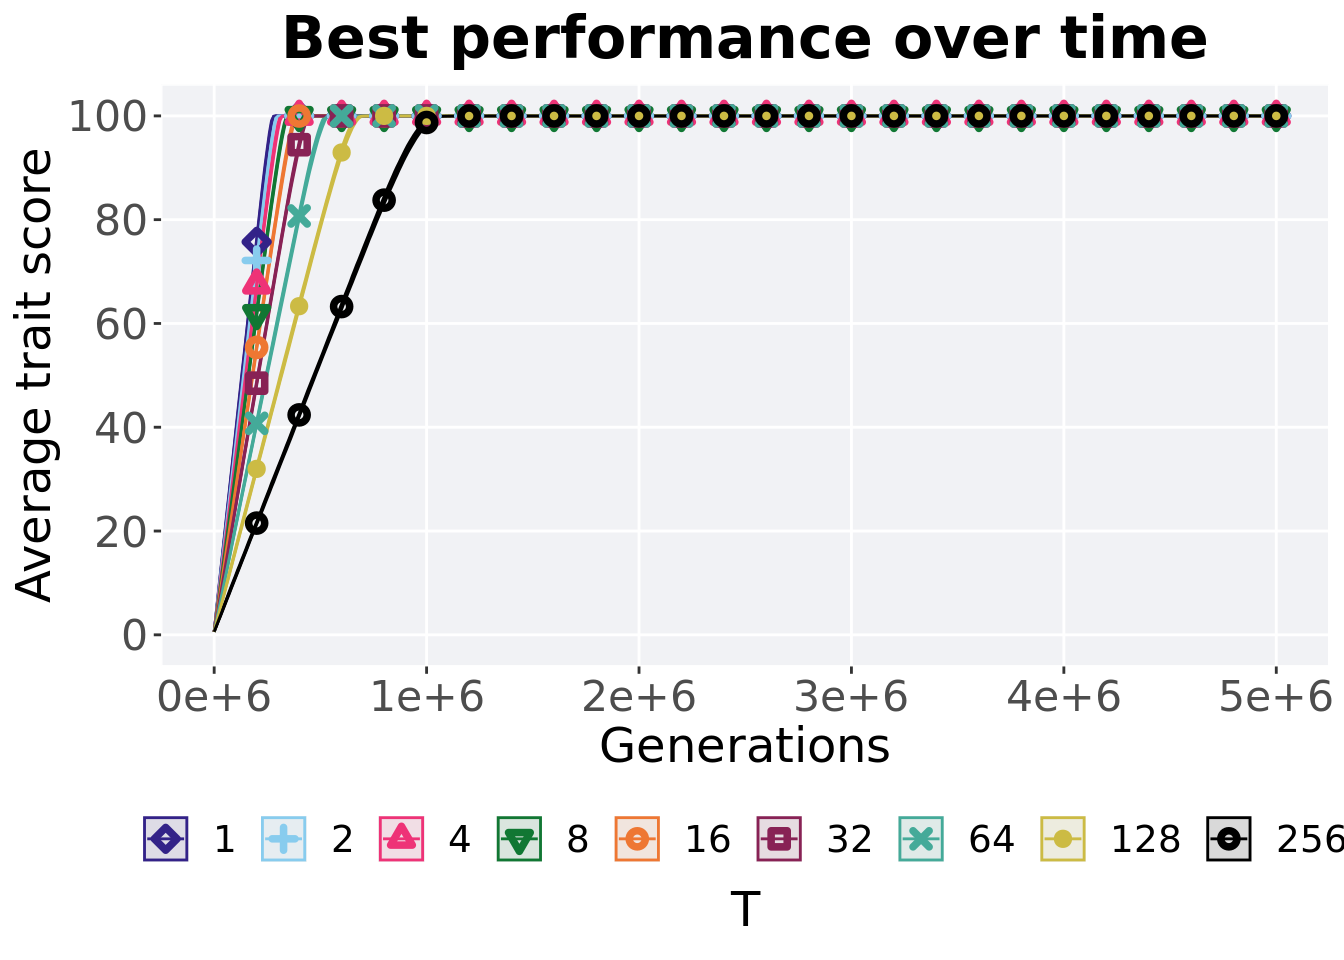
\includegraphics{demo_files/figure-latex/unnamed-chunk-77-1.pdf}

\hypertarget{generation-satisfactory-solution-found-3}{%
\subsection{Generation satisfactory solution found}\label{generation-satisfactory-solution-found-3}}

The first generation a satisfactory solution is found throughout the 50,000 generations.

\begin{Shaded}
\begin{Highlighting}[]
\NormalTok{ssf =}\StringTok{ }\KeywordTok{filter}\NormalTok{(tru_ssf, diagnostic }\OperatorTok{==}\StringTok{ 'ordered_exploitation'}\NormalTok{)}

\NormalTok{plot <-}\StringTok{ }\KeywordTok{ggplot}\NormalTok{(ssf, }\KeywordTok{aes}\NormalTok{(}\DataTypeTok{x =}\NormalTok{ T, }\DataTypeTok{y =}\NormalTok{ generation, }\DataTypeTok{color =}\NormalTok{ T, }\DataTypeTok{fill =}\NormalTok{ T, }\DataTypeTok{shape =}\NormalTok{ T)) }\OperatorTok{+}
\StringTok{  }\KeywordTok{geom_flat_violin}\NormalTok{(}\DataTypeTok{position =} \KeywordTok{position_nudge}\NormalTok{(}\DataTypeTok{x =} \FloatTok{.2}\NormalTok{, }\DataTypeTok{y =} \DecValTok{0}\NormalTok{), }\DataTypeTok{scale =} \StringTok{'width'}\NormalTok{, }\DataTypeTok{alpha =} \FloatTok{0.2}\NormalTok{) }\OperatorTok{+}
\StringTok{  }\KeywordTok{geom_point}\NormalTok{(}\DataTypeTok{position =} \KeywordTok{position_jitter}\NormalTok{(}\DataTypeTok{width =} \FloatTok{.1}\NormalTok{), }\DataTypeTok{size =} \FloatTok{1.5}\NormalTok{, }\DataTypeTok{alpha =} \FloatTok{1.0}\NormalTok{) }\OperatorTok{+}
\StringTok{  }\KeywordTok{geom_boxplot}\NormalTok{(}\DataTypeTok{color =} \StringTok{'black'}\NormalTok{, }\DataTypeTok{width =} \FloatTok{.2}\NormalTok{, }\DataTypeTok{outlier.shape =} \OtherTok{NA}\NormalTok{, }\DataTypeTok{alpha =} \FloatTok{0.0}\NormalTok{) }\OperatorTok{+}
\StringTok{  }\KeywordTok{scale_shape_manual}\NormalTok{(}\DataTypeTok{values=}\NormalTok{SHAPE)}\OperatorTok{+}
\StringTok{  }\KeywordTok{scale_y_continuous}\NormalTok{(}
    \DataTypeTok{name=}\StringTok{"Generation"}\NormalTok{,}
    \DataTypeTok{limits=}\KeywordTok{c}\NormalTok{(}\DecValTok{0}\NormalTok{, }\DecValTok{60000}\NormalTok{),}
    \DataTypeTok{breaks=}\KeywordTok{c}\NormalTok{(}\DecValTok{0}\NormalTok{, }\DecValTok{10000}\NormalTok{, }\DecValTok{20000}\NormalTok{, }\DecValTok{30000}\NormalTok{, }\DecValTok{40000}\NormalTok{, }\DecValTok{50000}\NormalTok{, }\DecValTok{60000}\NormalTok{),}
    \DataTypeTok{labels=}\KeywordTok{c}\NormalTok{(}\StringTok{"0e+6"}\NormalTok{, }\StringTok{"1e+6"}\NormalTok{, }\StringTok{"2e+6"}\NormalTok{, }\StringTok{"3e+6"}\NormalTok{, }\StringTok{"4e+6"}\NormalTok{, }\StringTok{"5e+6"}\NormalTok{, }\StringTok{"Fail"}\NormalTok{)}
\NormalTok{  ) }\OperatorTok{+}
\StringTok{  }\KeywordTok{scale_x_discrete}\NormalTok{(}
    \DataTypeTok{name=}\StringTok{"T"}
\NormalTok{  ) }\OperatorTok{+}
\StringTok{  }\KeywordTok{scale_colour_manual}\NormalTok{(}\DataTypeTok{values =}\NormalTok{ cb_palette) }\OperatorTok{+}
\StringTok{  }\KeywordTok{scale_fill_manual}\NormalTok{(}\DataTypeTok{values =}\NormalTok{ cb_palette) }\OperatorTok{+}
\StringTok{  }\NormalTok{p_theme}

\KeywordTok{plot_grid}\NormalTok{(}
\NormalTok{  plot }\OperatorTok{+}
\StringTok{    }\KeywordTok{ggtitle}\NormalTok{(}\StringTok{"Generation satisfactory solution found"}\NormalTok{) }\OperatorTok{+}
\StringTok{    }\KeywordTok{theme}\NormalTok{(}\DataTypeTok{legend.position=}\StringTok{"none"}\NormalTok{),}
\NormalTok{  legend,}
  \DataTypeTok{nrow=}\DecValTok{2}\NormalTok{,}
  \DataTypeTok{rel_heights =} \KeywordTok{c}\NormalTok{(}\DecValTok{2}\NormalTok{,.}\DecValTok{2}\NormalTok{),}
  \DataTypeTok{label_size =}\NormalTok{ TSIZE}
\NormalTok{)}
\end{Highlighting}
\end{Shaded}

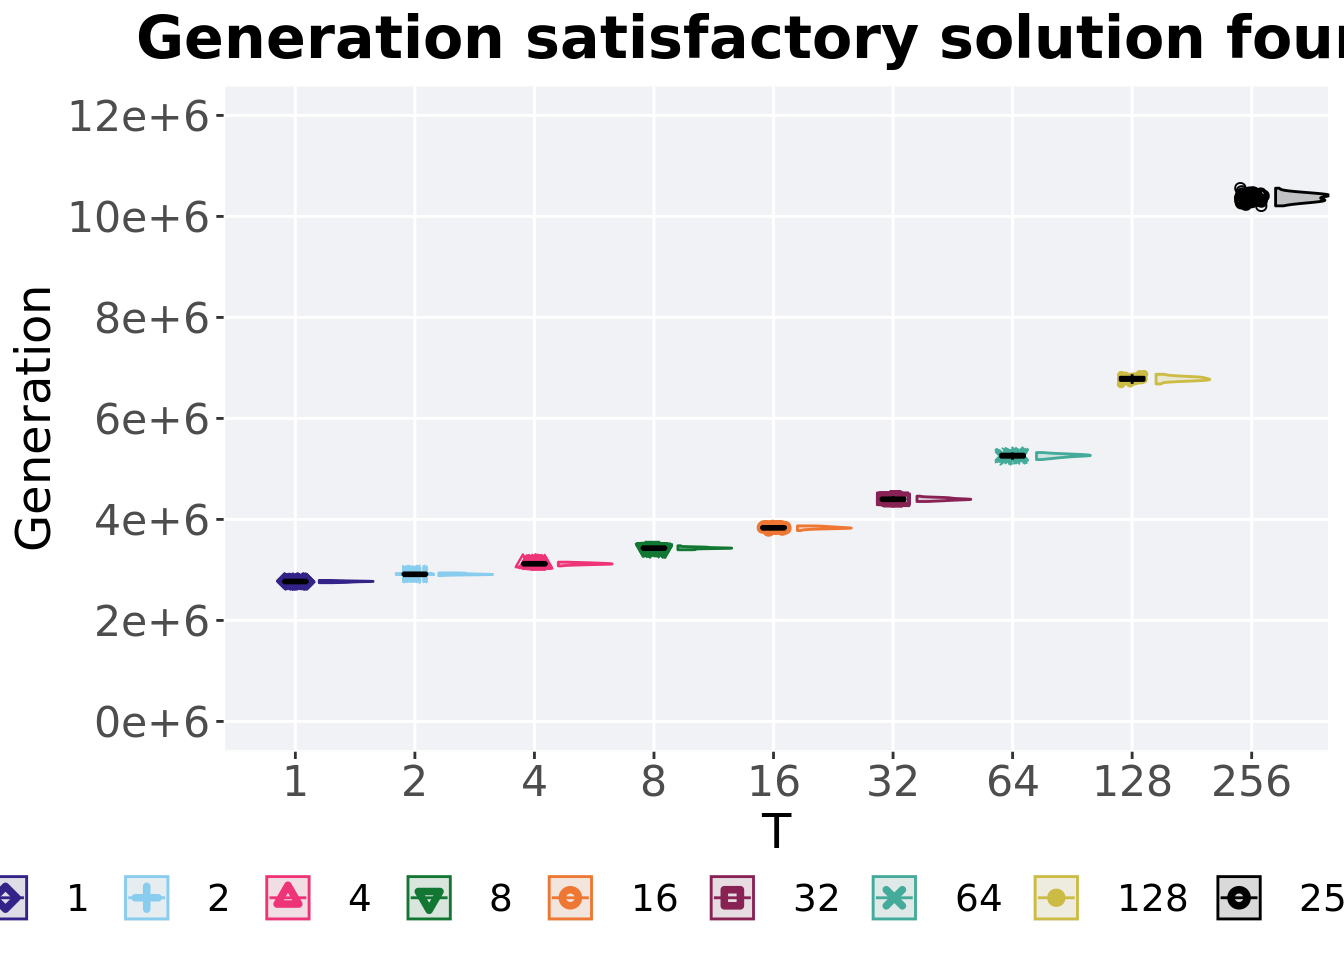
\includegraphics{demo_files/figure-latex/unnamed-chunk-79-1.pdf}

\hypertarget{stats-13}{%
\subsubsection{Stats}\label{stats-13}}

Summary statistics for the first generation a satisfactory solution is found throughout the 50,000 generations.

\begin{Shaded}
\begin{Highlighting}[]
\NormalTok{ssf =}\StringTok{ }\KeywordTok{filter}\NormalTok{(ssf, T }\OperatorTok{!=}\StringTok{ }\DecValTok{2}\NormalTok{)}

\KeywordTok{group_by}\NormalTok{(ssf, T) }\OperatorTok
\StringTok{  }\NormalTok{dplyr}\OperatorTok{::}\KeywordTok{summarise}\NormalTok{(}
    \DataTypeTok{count =} \KeywordTok{n}\NormalTok{(),}
    \DataTypeTok{na_cnt =} \KeywordTok{sum}\NormalTok{(}\KeywordTok{is.na}\NormalTok{(generation)),}
    \DataTypeTok{min =} \KeywordTok{min}\NormalTok{(generation, }\DataTypeTok{na.rm =} \OtherTok{TRUE}\NormalTok{),}
    \DataTypeTok{median =} \KeywordTok{median}\NormalTok{(generation, }\DataTypeTok{na.rm =} \OtherTok{TRUE}\NormalTok{),}
    \DataTypeTok{mean =} \KeywordTok{mean}\NormalTok{(generation, }\DataTypeTok{na.rm =} \OtherTok{TRUE}\NormalTok{),}
    \DataTypeTok{max =} \KeywordTok{max}\NormalTok{(generation, }\DataTypeTok{na.rm =} \OtherTok{TRUE}\NormalTok{),}
    \DataTypeTok{IQR =} \KeywordTok{IQR}\NormalTok{(generation, }\DataTypeTok{na.rm =} \OtherTok{TRUE}\NormalTok{)}
\NormalTok{  )}
\end{Highlighting}
\end{Shaded}

\begin{verbatim}
## # A tibble: 8 x 8
##   T     count na_cnt   min median   mean   max   IQR
##   <fct> <int>  <int> <dbl>  <dbl>  <dbl> <dbl> <dbl>
## 1 1        50      0 10460 11241  11172. 11869  409.
## 2 4        50      0 12720 13842  13830. 14809  448.
## 3 8        50      0 14487 15446. 15428. 16184  609.
## 4 16       50      0 16269 17168. 17103. 17969  566.
## 5 32       50      0 19009 20381  20332. 21414  606.
## 6 64       50      0 23993 25418. 25485. 26795  885.
## 7 128      50      0 35340 37772  37632. 39953 1039.
## 8 256      50      0 59999 59999  59999  59999    0
\end{verbatim}

Kruskal--Wallis test provides evidence of significant differences among the first generation a satisfactory solution is found throughout the 50,000 generations.

\begin{Shaded}
\begin{Highlighting}[]
\KeywordTok{kruskal.test}\NormalTok{(generation }\OperatorTok{~}\StringTok{ }\NormalTok{T, }\DataTypeTok{data =}\NormalTok{ ssf)}
\end{Highlighting}
\end{Shaded}

\begin{verbatim}
## 
##  Kruskal-Wallis rank sum test
## 
## data:  generation by T
## Kruskal-Wallis chi-squared = 393.51, df = 7, p-value < 2.2e-16
\end{verbatim}

Results for post-hoc Wilcoxon rank-sum test with a Bonferroni correction on the first generation a satisfactory solution is found throughout the 50,000 generations.

\begin{Shaded}
\begin{Highlighting}[]
\KeywordTok{pairwise.wilcox.test}\NormalTok{(}\DataTypeTok{x =}\NormalTok{ ssf}\OperatorTok{$}\NormalTok{generation, }\DataTypeTok{g =}\NormalTok{ ssf}\OperatorTok{$}\NormalTok{T , }\DataTypeTok{p.adjust.method =} \StringTok{"bonferroni"}\NormalTok{,}
                     \DataTypeTok{paired =} \OtherTok{FALSE}\NormalTok{, }\DataTypeTok{conf.int =} \OtherTok{FALSE}\NormalTok{, }\DataTypeTok{alternative =} \StringTok{'g'}\NormalTok{)}
\end{Highlighting}
\end{Shaded}

\begin{verbatim}
## 
##  Pairwise comparisons using Wilcoxon rank sum test with continuity correction 
## 
## data:  ssf$generation and ssf$T 
## 
##     1      4      8      16     32     64     128   
## 4   <2e-16 -      -      -      -      -      -     
## 8   <2e-16 <2e-16 -      -      -      -      -     
## 16  <2e-16 <2e-16 <2e-16 -      -      -      -     
## 32  <2e-16 <2e-16 <2e-16 <2e-16 -      -      -     
## 64  <2e-16 <2e-16 <2e-16 <2e-16 <2e-16 -      -     
## 128 <2e-16 <2e-16 <2e-16 <2e-16 <2e-16 <2e-16 -     
## 256 <2e-16 <2e-16 <2e-16 <2e-16 <2e-16 <2e-16 <2e-16
## 
## P value adjustment method: bonferroni
\end{verbatim}

\hypertarget{contraditruy-objectives-diagnostic}{%
\section{Contraditruy objectives diagnostic}\label{contraditruy-objectives-diagnostic}}

Here we present the results for \textbf{satisfactory trait coverage} and \textbf{activation gene coverage} found by each genotypic fitness sharing sigma value replicate on the ordered exploitation diagnostic.
Satisfactruy trait coverage refers to the count of unique satisfied traits in the population, while activation gene coverage refers to the count of unique activation genes in the population.
Note that both coverage values fall between 0 and 100.

\hypertarget{satisfactruy-trait-coverage}{%
\subsection{Satisfactruy trait coverage}\label{satisfactruy-trait-coverage}}

Satisfactruy trait coverage analysis.

\hypertarget{coverage-over-time-2}{%
\subsubsection{Coverage over time}\label{coverage-over-time-2}}

Satisfactruy trait coverage over time.

\begin{Shaded}
\begin{Highlighting}[]
\NormalTok{problem <-}\StringTok{ }\KeywordTok{filter}\NormalTok{(tru_ot, diagnostic }\OperatorTok{==}\StringTok{ 'contradictory_objectives'}\NormalTok{)}
\NormalTok{lines =}\StringTok{ }\NormalTok{problem }\OperatorTok
\StringTok{        }\KeywordTok{group_by}\NormalTok{(T, gen) }\OperatorTok
\StringTok{          }\NormalTok{dplyr}\OperatorTok{::}\KeywordTok{summarise}\NormalTok{(}
            \DataTypeTok{min =} \KeywordTok{min}\NormalTok{(pop_uni_obj),}
            \DataTypeTok{mean =} \KeywordTok{mean}\NormalTok{(pop_uni_obj),}
            \DataTypeTok{max =} \KeywordTok{max}\NormalTok{(pop_uni_obj)}
\NormalTok{          )}
\end{Highlighting}
\end{Shaded}

\begin{verbatim}
## `summarise()` has grouped output by 'T'. You can override using the `.groups`
## argument.
\end{verbatim}

\begin{Shaded}
\begin{Highlighting}[]
\NormalTok{points =}\StringTok{ }\KeywordTok{filter}\NormalTok{(lines, gen }\OperatorTok\StringTok{ }\DecValTok{2000} \OperatorTok{==}\StringTok{ }\DecValTok{0} \OperatorTok{&}\StringTok{ }\NormalTok{gen }\OperatorTok{!=}\StringTok{ }\DecValTok{0}\NormalTok{)}

\NormalTok{ot =}\StringTok{ }\KeywordTok{ggplot}\NormalTok{(lines, }\KeywordTok{aes}\NormalTok{(}\DataTypeTok{x=}\NormalTok{gen, }\DataTypeTok{y=}\NormalTok{mean, }\DataTypeTok{group =}\NormalTok{ T, }\DataTypeTok{fill =}\NormalTok{T, }\DataTypeTok{color =}\NormalTok{ T, }\DataTypeTok{shape =}\NormalTok{ T)) }\OperatorTok{+}
\StringTok{  }\KeywordTok{geom_ribbon}\NormalTok{(}\KeywordTok{aes}\NormalTok{(}\DataTypeTok{ymin =}\NormalTok{ min, }\DataTypeTok{ymax =}\NormalTok{ max), }\DataTypeTok{alpha =} \FloatTok{0.1}\NormalTok{) }\OperatorTok{+}
\StringTok{  }\KeywordTok{geom_line}\NormalTok{(}\DataTypeTok{size =} \FloatTok{0.5}\NormalTok{) }\OperatorTok{+}
\StringTok{  }\KeywordTok{geom_point}\NormalTok{(}\DataTypeTok{data =}\NormalTok{ points, }\DataTypeTok{size =} \FloatTok{1.5}\NormalTok{, }\DataTypeTok{stroke =} \FloatTok{2.0}\NormalTok{, }\DataTypeTok{alpha =} \FloatTok{1.0}\NormalTok{) }\OperatorTok{+}
\StringTok{  }\KeywordTok{scale_y_continuous}\NormalTok{(}
    \DataTypeTok{name=}\StringTok{"Coverage"}\NormalTok{,}
    \DataTypeTok{limits=}\KeywordTok{c}\NormalTok{(}\DecValTok{0}\NormalTok{, }\DecValTok{5}\NormalTok{)}
\NormalTok{  ) }\OperatorTok{+}
\StringTok{  }\KeywordTok{scale_x_continuous}\NormalTok{(}
    \DataTypeTok{name=}\StringTok{"Generations"}\NormalTok{,}
    \DataTypeTok{limits=}\KeywordTok{c}\NormalTok{(}\DecValTok{0}\NormalTok{, }\DecValTok{50000}\NormalTok{),}
    \DataTypeTok{breaks=}\KeywordTok{c}\NormalTok{(}\DecValTok{0}\NormalTok{, }\DecValTok{10000}\NormalTok{, }\DecValTok{20000}\NormalTok{, }\DecValTok{30000}\NormalTok{, }\DecValTok{40000}\NormalTok{, }\DecValTok{50000}\NormalTok{),}
    \DataTypeTok{labels=}\KeywordTok{c}\NormalTok{(}\StringTok{"0e+6"}\NormalTok{, }\StringTok{"1e+6"}\NormalTok{, }\StringTok{"2e+6"}\NormalTok{, }\StringTok{"3e+6"}\NormalTok{, }\StringTok{"4e+6"}\NormalTok{, }\StringTok{"5e+6"}\NormalTok{)}

\NormalTok{  ) }\OperatorTok{+}
\StringTok{  }\KeywordTok{scale_shape_manual}\NormalTok{(}\DataTypeTok{values=}\NormalTok{SHAPE)}\OperatorTok{+}
\StringTok{  }\KeywordTok{scale_colour_manual}\NormalTok{(}\DataTypeTok{values =}\NormalTok{ cb_palette) }\OperatorTok{+}
\StringTok{  }\KeywordTok{scale_fill_manual}\NormalTok{(}\DataTypeTok{values =}\NormalTok{ cb_palette) }\OperatorTok{+}
\StringTok{  }\KeywordTok{ggtitle}\NormalTok{(}\StringTok{"Satisfactruy trait coverage over time"}\NormalTok{) }\OperatorTok{+}
\StringTok{  }\NormalTok{p_theme}\OperatorTok{+}
\StringTok{    }\KeywordTok{guides}\NormalTok{(}
    \DataTypeTok{shape=}\KeywordTok{guide_legend}\NormalTok{(}\DataTypeTok{nrow=}\DecValTok{1}\NormalTok{, }\DataTypeTok{title.position =} \StringTok{"bottom"}\NormalTok{),}
    \DataTypeTok{color=}\KeywordTok{guide_legend}\NormalTok{(}\DataTypeTok{nrow=}\DecValTok{1}\NormalTok{, }\DataTypeTok{title.position =} \StringTok{"bottom"}\NormalTok{),}
    \DataTypeTok{fill=}\KeywordTok{guide_legend}\NormalTok{(}\DataTypeTok{nrow=}\DecValTok{1}\NormalTok{, }\DataTypeTok{title.position =} \StringTok{"bottom"}\NormalTok{)}
\NormalTok{  ) }\OperatorTok{+}
\StringTok{  }\KeywordTok{theme}\NormalTok{(}
    \DataTypeTok{legend.position =} \StringTok{"bottom"}\NormalTok{,}
    \DataTypeTok{legend.box=}\StringTok{"verticle"}\NormalTok{,}
    \DataTypeTok{legend.justification=}\StringTok{"center"}\NormalTok{,}
    \DataTypeTok{legend.title.align=}\FloatTok{0.5}
\NormalTok{  )}

\NormalTok{ot}
\end{Highlighting}
\end{Shaded}

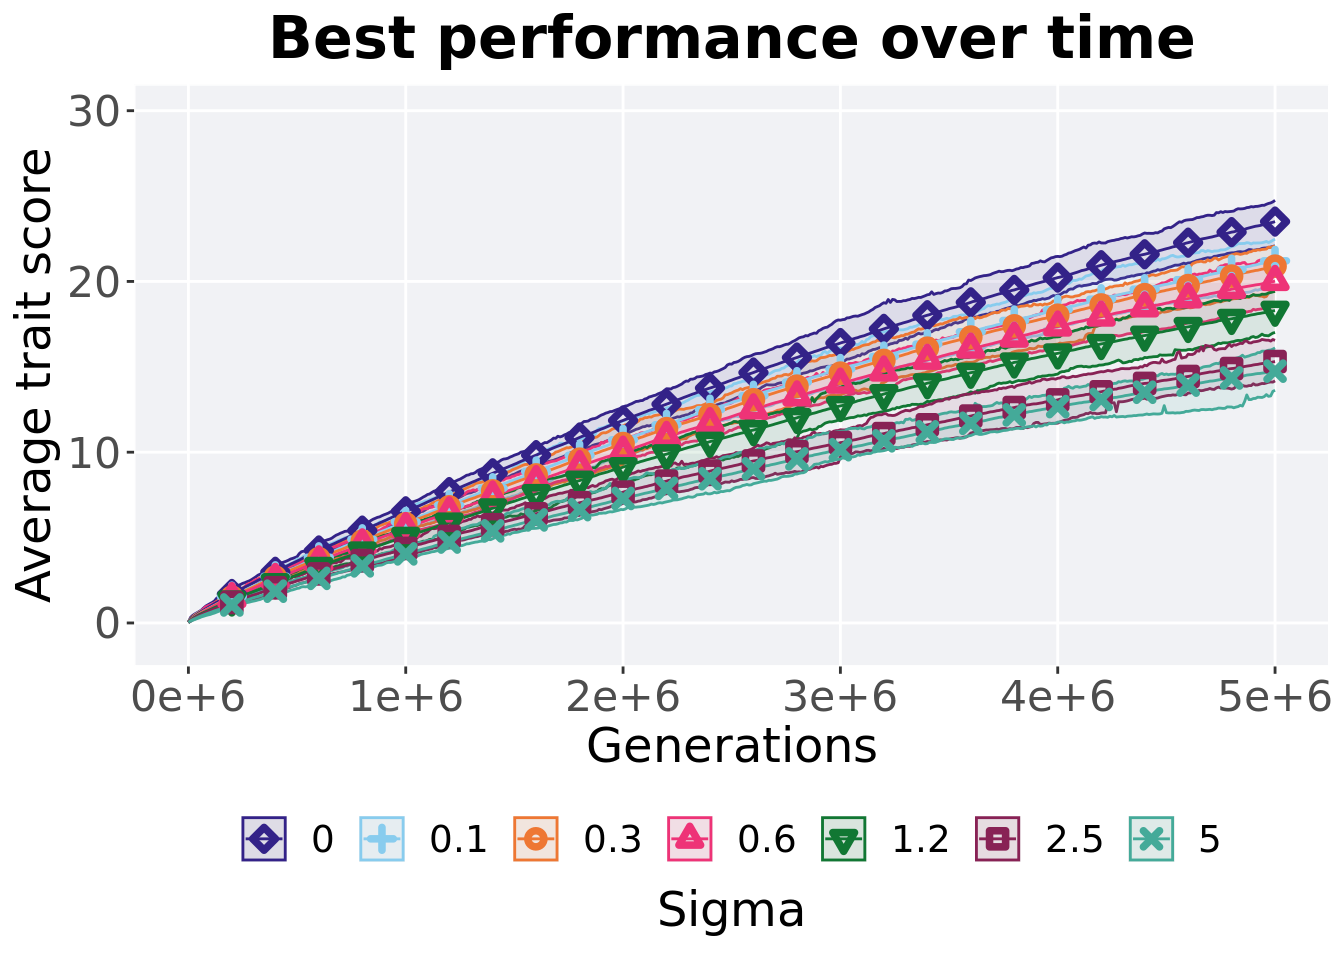
\includegraphics{demo_files/figure-latex/unnamed-chunk-83-1.pdf}

\hypertarget{best-coverage-throughout-2}{%
\subsubsection{Best coverage throughout}\label{best-coverage-throughout-2}}

Best satisfactory trait coverage throughout 50,000 generations.

\begin{Shaded}
\begin{Highlighting}[]
\NormalTok{best =}\StringTok{ }\KeywordTok{filter}\NormalTok{(tru_best, col }\OperatorTok{==}\StringTok{ 'pop_uni_obj'} \OperatorTok{&}\StringTok{ }\NormalTok{diagnostic }\OperatorTok{==}\StringTok{ 'contradictory_objectives'}\NormalTok{)}

\NormalTok{plot =}\StringTok{ }\KeywordTok{ggplot}\NormalTok{(best, }\KeywordTok{aes}\NormalTok{(}\DataTypeTok{x =}\NormalTok{ T, }\DataTypeTok{y =}\NormalTok{ val, }\DataTypeTok{color =}\NormalTok{ T, }\DataTypeTok{fill =}\NormalTok{ T, }\DataTypeTok{shape =}\NormalTok{ T)) }\OperatorTok{+}
\StringTok{  }\KeywordTok{geom_flat_violin}\NormalTok{(}\DataTypeTok{position =} \KeywordTok{position_nudge}\NormalTok{(}\DataTypeTok{x =} \FloatTok{.2}\NormalTok{, }\DataTypeTok{y =} \DecValTok{0}\NormalTok{), }\DataTypeTok{scale =} \StringTok{'width'}\NormalTok{, }\DataTypeTok{alpha =} \FloatTok{0.2}\NormalTok{) }\OperatorTok{+}
\StringTok{  }\KeywordTok{geom_point}\NormalTok{(}\DataTypeTok{position =} \KeywordTok{position_jitter}\NormalTok{(}\DataTypeTok{width =} \FloatTok{.1}\NormalTok{), }\DataTypeTok{size =} \FloatTok{1.5}\NormalTok{, }\DataTypeTok{alpha =} \FloatTok{1.0}\NormalTok{) }\OperatorTok{+}
\StringTok{  }\KeywordTok{geom_boxplot}\NormalTok{(}\DataTypeTok{color =} \StringTok{'black'}\NormalTok{, }\DataTypeTok{width =} \FloatTok{.2}\NormalTok{, }\DataTypeTok{outlier.shape =} \OtherTok{NA}\NormalTok{, }\DataTypeTok{alpha =} \FloatTok{0.0}\NormalTok{) }\OperatorTok{+}
\StringTok{  }\KeywordTok{scale_y_continuous}\NormalTok{(}
    \DataTypeTok{name=}\StringTok{"Coverage"}\NormalTok{,}
    \DataTypeTok{limits=}\KeywordTok{c}\NormalTok{(}\DecValTok{0}\NormalTok{, }\DecValTok{5}\NormalTok{)}
\NormalTok{  ) }\OperatorTok{+}
\StringTok{  }\KeywordTok{scale_x_discrete}\NormalTok{(}
    \DataTypeTok{name=}\StringTok{"T"}
\NormalTok{  )}\OperatorTok{+}
\StringTok{  }\KeywordTok{scale_shape_manual}\NormalTok{(}\DataTypeTok{values=}\NormalTok{SHAPE)}\OperatorTok{+}
\StringTok{  }\KeywordTok{scale_colour_manual}\NormalTok{(}\DataTypeTok{values =}\NormalTok{ cb_palette) }\OperatorTok{+}
\StringTok{  }\KeywordTok{scale_fill_manual}\NormalTok{(}\DataTypeTok{values =}\NormalTok{ cb_palette) }\OperatorTok{+}
\StringTok{  }\NormalTok{p_theme}

\KeywordTok{plot_grid}\NormalTok{(}
\NormalTok{  plot }\OperatorTok{+}
\StringTok{    }\KeywordTok{ggtitle}\NormalTok{(}\StringTok{"Best satisfactory trait coverage"}\NormalTok{) }\OperatorTok{+}
\StringTok{    }\KeywordTok{theme}\NormalTok{(}\DataTypeTok{legend.position=}\StringTok{"none"}\NormalTok{),}
\NormalTok{  legend,}
  \DataTypeTok{nrow=}\DecValTok{2}\NormalTok{,}
  \DataTypeTok{rel_heights =} \KeywordTok{c}\NormalTok{(}\DecValTok{2}\NormalTok{,.}\DecValTok{2}\NormalTok{),}
  \DataTypeTok{label_size =}\NormalTok{ TSIZE}
\NormalTok{)}
\end{Highlighting}
\end{Shaded}

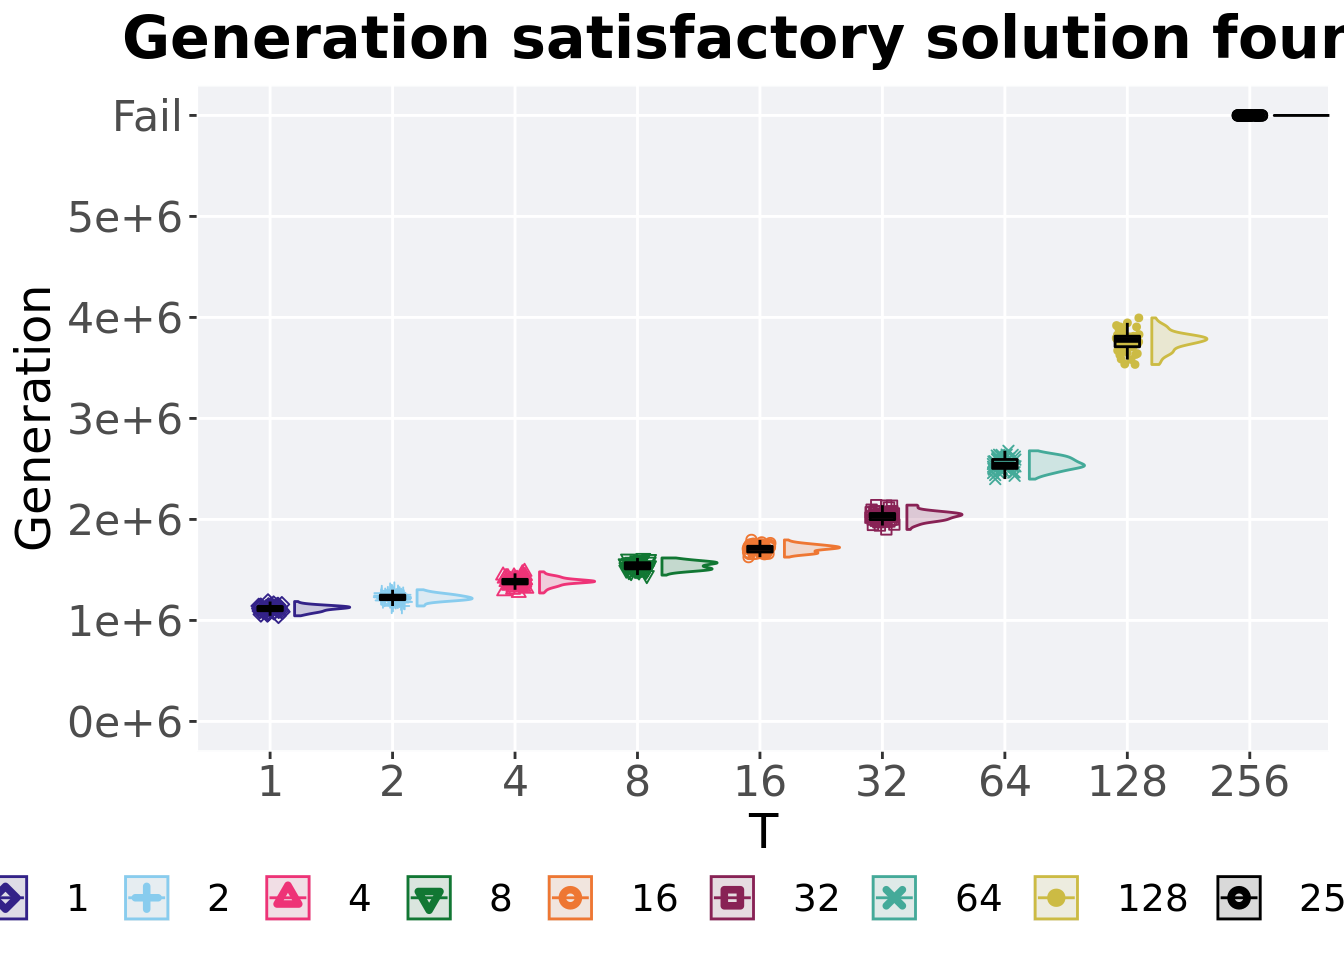
\includegraphics{demo_files/figure-latex/unnamed-chunk-85-1.pdf}

\hypertarget{stats-14}{%
\paragraph{Stats}\label{stats-14}}

Summary statistics for the best satisfactory trait coverage throughout 50,000 generations.

\begin{Shaded}
\begin{Highlighting}[]
\KeywordTok{group_by}\NormalTok{(best, T) }\OperatorTok
\StringTok{  }\NormalTok{dplyr}\OperatorTok{::}\KeywordTok{summarise}\NormalTok{(}
    \DataTypeTok{count =} \KeywordTok{n}\NormalTok{(),}
    \DataTypeTok{na_cnt =} \KeywordTok{sum}\NormalTok{(}\KeywordTok{is.na}\NormalTok{(val)),}
    \DataTypeTok{min =} \KeywordTok{min}\NormalTok{(val, }\DataTypeTok{na.rm =} \OtherTok{TRUE}\NormalTok{),}
    \DataTypeTok{median =} \KeywordTok{median}\NormalTok{(val, }\DataTypeTok{na.rm =} \OtherTok{TRUE}\NormalTok{),}
    \DataTypeTok{mean =} \KeywordTok{mean}\NormalTok{(val, }\DataTypeTok{na.rm =} \OtherTok{TRUE}\NormalTok{),}
    \DataTypeTok{max =} \KeywordTok{max}\NormalTok{(val, }\DataTypeTok{na.rm =} \OtherTok{TRUE}\NormalTok{),}
    \DataTypeTok{IQR =} \KeywordTok{IQR}\NormalTok{(val, }\DataTypeTok{na.rm =} \OtherTok{TRUE}\NormalTok{)}
\NormalTok{  )}
\end{Highlighting}
\end{Shaded}

\begin{verbatim}
## # A tibble: 9 x 8
##   T     count na_cnt   min median  mean   max   IQR
##   <fct> <int>  <int> <dbl>  <dbl> <dbl> <dbl> <dbl>
## 1 1        50      0     1      1     1     1     0
## 2 2        50      0     1      1     1     1     0
## 3 4        50      0     1      1     1     1     0
## 4 8        50      0     1      1     1     1     0
## 5 16       50      0     1      1     1     1     0
## 6 32       50      0     1      1     1     1     0
## 7 64       50      0     1      1     1     1     0
## 8 128      50      0     1      1     1     1     0
## 9 256      50      0     1      1     1     1     0
\end{verbatim}

\hypertarget{end-of-50000-generations-5}{%
\subsubsection{End of 50,000 generations}\label{end-of-50000-generations-5}}

Satisfactruy trait coverage in the population at the end of 50,000 generations.

\begin{Shaded}
\begin{Highlighting}[]
\NormalTok{end =}\StringTok{ }\KeywordTok{filter}\NormalTok{(tru_end, diagnostic }\OperatorTok{==}\StringTok{ 'contradictory_objectives'}\NormalTok{)}
\NormalTok{plot =}\StringTok{ }\KeywordTok{ggplot}\NormalTok{(end, }\KeywordTok{aes}\NormalTok{(}\DataTypeTok{x =}\NormalTok{ T, }\DataTypeTok{y =}\NormalTok{ pop_uni_obj, }\DataTypeTok{color =}\NormalTok{ T, }\DataTypeTok{fill =}\NormalTok{ T, }\DataTypeTok{shape =}\NormalTok{ T)) }\OperatorTok{+}
\StringTok{  }\KeywordTok{geom_flat_violin}\NormalTok{(}\DataTypeTok{position =} \KeywordTok{position_nudge}\NormalTok{(}\DataTypeTok{x =} \FloatTok{.2}\NormalTok{, }\DataTypeTok{y =} \DecValTok{0}\NormalTok{), }\DataTypeTok{scale =} \StringTok{'width'}\NormalTok{, }\DataTypeTok{alpha =} \FloatTok{0.2}\NormalTok{) }\OperatorTok{+}
\StringTok{  }\KeywordTok{geom_point}\NormalTok{(}\DataTypeTok{position =} \KeywordTok{position_jitter}\NormalTok{(}\DataTypeTok{width =} \FloatTok{.1}\NormalTok{), }\DataTypeTok{size =} \FloatTok{1.5}\NormalTok{, }\DataTypeTok{alpha =} \FloatTok{1.0}\NormalTok{) }\OperatorTok{+}
\StringTok{  }\KeywordTok{geom_boxplot}\NormalTok{(}\DataTypeTok{color =} \StringTok{'black'}\NormalTok{, }\DataTypeTok{width =} \FloatTok{.2}\NormalTok{, }\DataTypeTok{outlier.shape =} \OtherTok{NA}\NormalTok{, }\DataTypeTok{alpha =} \FloatTok{0.0}\NormalTok{) }\OperatorTok{+}
\StringTok{  }\KeywordTok{scale_y_continuous}\NormalTok{(}
    \DataTypeTok{name=}\StringTok{"Coverage"}\NormalTok{,}
    \DataTypeTok{limits=}\KeywordTok{c}\NormalTok{(}\DecValTok{0}\NormalTok{, }\DecValTok{5}\NormalTok{)}
\NormalTok{  ) }\OperatorTok{+}
\StringTok{  }\KeywordTok{scale_x_discrete}\NormalTok{(}
    \DataTypeTok{name=}\StringTok{"T"}
\NormalTok{  )}\OperatorTok{+}
\StringTok{  }\KeywordTok{scale_shape_manual}\NormalTok{(}\DataTypeTok{values=}\NormalTok{SHAPE)}\OperatorTok{+}
\StringTok{  }\KeywordTok{scale_colour_manual}\NormalTok{(}\DataTypeTok{values =}\NormalTok{ cb_palette) }\OperatorTok{+}
\StringTok{  }\KeywordTok{scale_fill_manual}\NormalTok{(}\DataTypeTok{values =}\NormalTok{ cb_palette) }\OperatorTok{+}
\StringTok{  }\NormalTok{p_theme}

\KeywordTok{plot_grid}\NormalTok{(}
\NormalTok{  plot }\OperatorTok{+}
\StringTok{    }\KeywordTok{ggtitle}\NormalTok{(}\StringTok{"Final satisfactory trait coverage"}\NormalTok{) }\OperatorTok{+}
\StringTok{    }\KeywordTok{theme}\NormalTok{(}\DataTypeTok{legend.position=}\StringTok{"none"}\NormalTok{),}
\NormalTok{  legend,}
  \DataTypeTok{nrow=}\DecValTok{2}\NormalTok{,}
  \DataTypeTok{rel_heights =} \KeywordTok{c}\NormalTok{(}\DecValTok{2}\NormalTok{,.}\DecValTok{3}\NormalTok{),}
  \DataTypeTok{label_size =}\NormalTok{ TSIZE}
\NormalTok{)}
\end{Highlighting}
\end{Shaded}

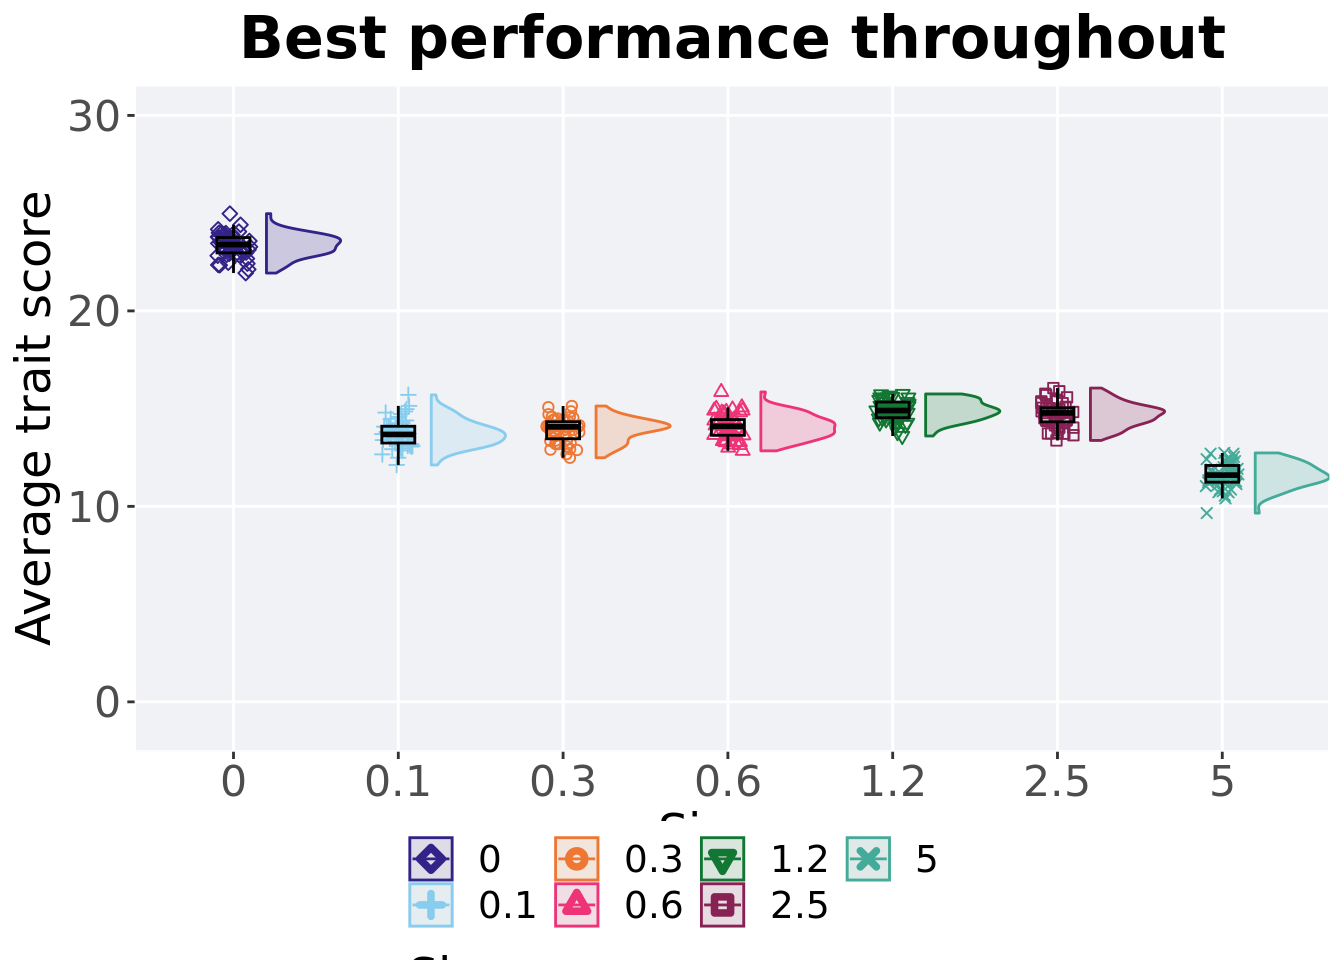
\includegraphics{demo_files/figure-latex/unnamed-chunk-87-1.pdf}

\hypertarget{stats-15}{%
\paragraph{Stats}\label{stats-15}}

Summary statistics for satisfactory trait coverage in the population at the end of 50,000 generations.

\begin{Shaded}
\begin{Highlighting}[]
\KeywordTok{group_by}\NormalTok{(end, T) }\OperatorTok
\StringTok{  }\NormalTok{dplyr}\OperatorTok{::}\KeywordTok{summarise}\NormalTok{(}
    \DataTypeTok{count =} \KeywordTok{n}\NormalTok{(),}
    \DataTypeTok{na_cnt =} \KeywordTok{sum}\NormalTok{(}\KeywordTok{is.na}\NormalTok{(pop_uni_obj)),}
    \DataTypeTok{min =} \KeywordTok{min}\NormalTok{(pop_uni_obj, }\DataTypeTok{na.rm =} \OtherTok{TRUE}\NormalTok{),}
    \DataTypeTok{median =} \KeywordTok{median}\NormalTok{(pop_uni_obj, }\DataTypeTok{na.rm =} \OtherTok{TRUE}\NormalTok{),}
    \DataTypeTok{mean =} \KeywordTok{mean}\NormalTok{(pop_uni_obj, }\DataTypeTok{na.rm =} \OtherTok{TRUE}\NormalTok{),}
    \DataTypeTok{max =} \KeywordTok{max}\NormalTok{(pop_uni_obj, }\DataTypeTok{na.rm =} \OtherTok{TRUE}\NormalTok{),}
    \DataTypeTok{IQR =} \KeywordTok{IQR}\NormalTok{(pop_uni_obj, }\DataTypeTok{na.rm =} \OtherTok{TRUE}\NormalTok{)}
\NormalTok{  )}
\end{Highlighting}
\end{Shaded}

\begin{verbatim}
## # A tibble: 9 x 8
##   T     count na_cnt   min median  mean   max   IQR
##   <fct> <int>  <int> <int>  <dbl> <dbl> <int> <dbl>
## 1 1        50      0     1      1     1     1     0
## 2 2        50      0     1      1     1     1     0
## 3 4        50      0     1      1     1     1     0
## 4 8        50      0     1      1     1     1     0
## 5 16       50      0     1      1     1     1     0
## 6 32       50      0     1      1     1     1     0
## 7 64       50      0     1      1     1     1     0
## 8 128      50      0     1      1     1     1     0
## 9 256      50      0     1      1     1     1     0
\end{verbatim}

\hypertarget{activation-gene-coverage-2}{%
\subsection{Activation gene coverage}\label{activation-gene-coverage-2}}

Here we analyze the activation gene coverage for each parameter replicate on the contradictory objectives diagnostic.

\hypertarget{coverage-over-time-3}{%
\subsubsection{Coverage over time}\label{coverage-over-time-3}}

Activation gene coverage over time.

\begin{Shaded}
\begin{Highlighting}[]
\NormalTok{problem <-}\StringTok{ }\KeywordTok{filter}\NormalTok{(tru_ot, diagnostic }\OperatorTok{==}\StringTok{ 'contradictory_objectives'}\NormalTok{)}
\NormalTok{lines =}\StringTok{ }\NormalTok{problem }\OperatorTok
\StringTok{        }\KeywordTok{group_by}\NormalTok{(T, gen) }\OperatorTok
\StringTok{          }\NormalTok{dplyr}\OperatorTok{::}\KeywordTok{summarise}\NormalTok{(}
            \DataTypeTok{min =} \KeywordTok{min}\NormalTok{(uni_str_pos),}
            \DataTypeTok{mean =} \KeywordTok{mean}\NormalTok{(uni_str_pos),}
            \DataTypeTok{max =} \KeywordTok{max}\NormalTok{(uni_str_pos)}
\NormalTok{          )}
\end{Highlighting}
\end{Shaded}

\begin{verbatim}
## `summarise()` has grouped output by 'T'. You can override using the `.groups`
## argument.
\end{verbatim}

\begin{Shaded}
\begin{Highlighting}[]
\NormalTok{points =}\StringTok{ }\KeywordTok{filter}\NormalTok{(lines, gen }\OperatorTok\StringTok{ }\DecValTok{2000} \OperatorTok{==}\StringTok{ }\DecValTok{0} \OperatorTok{&}\StringTok{ }\NormalTok{gen }\OperatorTok{!=}\StringTok{ }\DecValTok{0}\NormalTok{)}

\NormalTok{ot =}\StringTok{ }\KeywordTok{ggplot}\NormalTok{(lines, }\KeywordTok{aes}\NormalTok{(}\DataTypeTok{x=}\NormalTok{gen, }\DataTypeTok{y=}\NormalTok{mean, }\DataTypeTok{group =}\NormalTok{ T, }\DataTypeTok{fill =}\NormalTok{T, }\DataTypeTok{color =}\NormalTok{ T, }\DataTypeTok{shape =}\NormalTok{ T)) }\OperatorTok{+}
\StringTok{  }\KeywordTok{geom_ribbon}\NormalTok{(}\KeywordTok{aes}\NormalTok{(}\DataTypeTok{ymin =}\NormalTok{ min, }\DataTypeTok{ymax =}\NormalTok{ max), }\DataTypeTok{alpha =} \FloatTok{0.1}\NormalTok{) }\OperatorTok{+}
\StringTok{  }\KeywordTok{geom_line}\NormalTok{(}\DataTypeTok{size =} \FloatTok{0.5}\NormalTok{) }\OperatorTok{+}
\StringTok{  }\KeywordTok{geom_point}\NormalTok{(}\DataTypeTok{data =}\NormalTok{ points, }\DataTypeTok{size =} \FloatTok{1.5}\NormalTok{, }\DataTypeTok{stroke =} \FloatTok{2.0}\NormalTok{, }\DataTypeTok{alpha =} \FloatTok{1.0}\NormalTok{) }\OperatorTok{+}
\StringTok{  }\KeywordTok{scale_y_continuous}\NormalTok{(}
    \DataTypeTok{name=}\StringTok{"Coverage"}\NormalTok{,}
    \DataTypeTok{limits=}\KeywordTok{c}\NormalTok{(}\OperatorTok{-}\DecValTok{1}\NormalTok{, }\DecValTok{101}\NormalTok{),}
    \DataTypeTok{breaks=}\KeywordTok{seq}\NormalTok{(}\DecValTok{0}\NormalTok{,}\DecValTok{100}\NormalTok{, }\DecValTok{20}\NormalTok{),}
    \DataTypeTok{labels=}\KeywordTok{c}\NormalTok{(}\StringTok{"0"}\NormalTok{, }\StringTok{"20"}\NormalTok{, }\StringTok{"40"}\NormalTok{, }\StringTok{"60"}\NormalTok{, }\StringTok{"80"}\NormalTok{, }\StringTok{"100"}\NormalTok{)}
\NormalTok{  ) }\OperatorTok{+}
\StringTok{  }\KeywordTok{scale_x_continuous}\NormalTok{(}
    \DataTypeTok{name=}\StringTok{"Generations"}\NormalTok{,}
    \DataTypeTok{limits=}\KeywordTok{c}\NormalTok{(}\DecValTok{0}\NormalTok{, }\DecValTok{50000}\NormalTok{),}
    \DataTypeTok{breaks=}\KeywordTok{c}\NormalTok{(}\DecValTok{0}\NormalTok{, }\DecValTok{10000}\NormalTok{, }\DecValTok{20000}\NormalTok{, }\DecValTok{30000}\NormalTok{, }\DecValTok{40000}\NormalTok{, }\DecValTok{50000}\NormalTok{),}
    \DataTypeTok{labels=}\KeywordTok{c}\NormalTok{(}\StringTok{"0e+6"}\NormalTok{, }\StringTok{"1e+6"}\NormalTok{, }\StringTok{"2e+6"}\NormalTok{, }\StringTok{"3e+6"}\NormalTok{, }\StringTok{"4e+6"}\NormalTok{, }\StringTok{"5e+6"}\NormalTok{)}

\NormalTok{  ) }\OperatorTok{+}
\StringTok{  }\KeywordTok{scale_shape_manual}\NormalTok{(}\DataTypeTok{values=}\NormalTok{SHAPE)}\OperatorTok{+}
\StringTok{  }\KeywordTok{scale_colour_manual}\NormalTok{(}\DataTypeTok{values =}\NormalTok{ cb_palette) }\OperatorTok{+}
\StringTok{  }\KeywordTok{scale_fill_manual}\NormalTok{(}\DataTypeTok{values =}\NormalTok{ cb_palette) }\OperatorTok{+}
\StringTok{  }\KeywordTok{ggtitle}\NormalTok{(}\StringTok{"Activation gene coverage over time"}\NormalTok{) }\OperatorTok{+}
\StringTok{  }\NormalTok{p_theme}\OperatorTok{+}
\StringTok{    }\KeywordTok{guides}\NormalTok{(}
    \DataTypeTok{shape=}\KeywordTok{guide_legend}\NormalTok{(}\DataTypeTok{nrow=}\DecValTok{1}\NormalTok{, }\DataTypeTok{title.position =} \StringTok{"bottom"}\NormalTok{),}
    \DataTypeTok{color=}\KeywordTok{guide_legend}\NormalTok{(}\DataTypeTok{nrow=}\DecValTok{1}\NormalTok{, }\DataTypeTok{title.position =} \StringTok{"bottom"}\NormalTok{),}
    \DataTypeTok{fill=}\KeywordTok{guide_legend}\NormalTok{(}\DataTypeTok{nrow=}\DecValTok{1}\NormalTok{, }\DataTypeTok{title.position =} \StringTok{"bottom"}\NormalTok{)}
\NormalTok{  ) }\OperatorTok{+}
\StringTok{  }\KeywordTok{theme}\NormalTok{(}
    \DataTypeTok{legend.position =} \StringTok{"bottom"}\NormalTok{,}
    \DataTypeTok{legend.box=}\StringTok{"verticle"}\NormalTok{,}
    \DataTypeTok{legend.justification=}\StringTok{"center"}\NormalTok{,}
    \DataTypeTok{legend.title.align=}\FloatTok{0.5}
\NormalTok{  )}

\NormalTok{ot}
\end{Highlighting}
\end{Shaded}

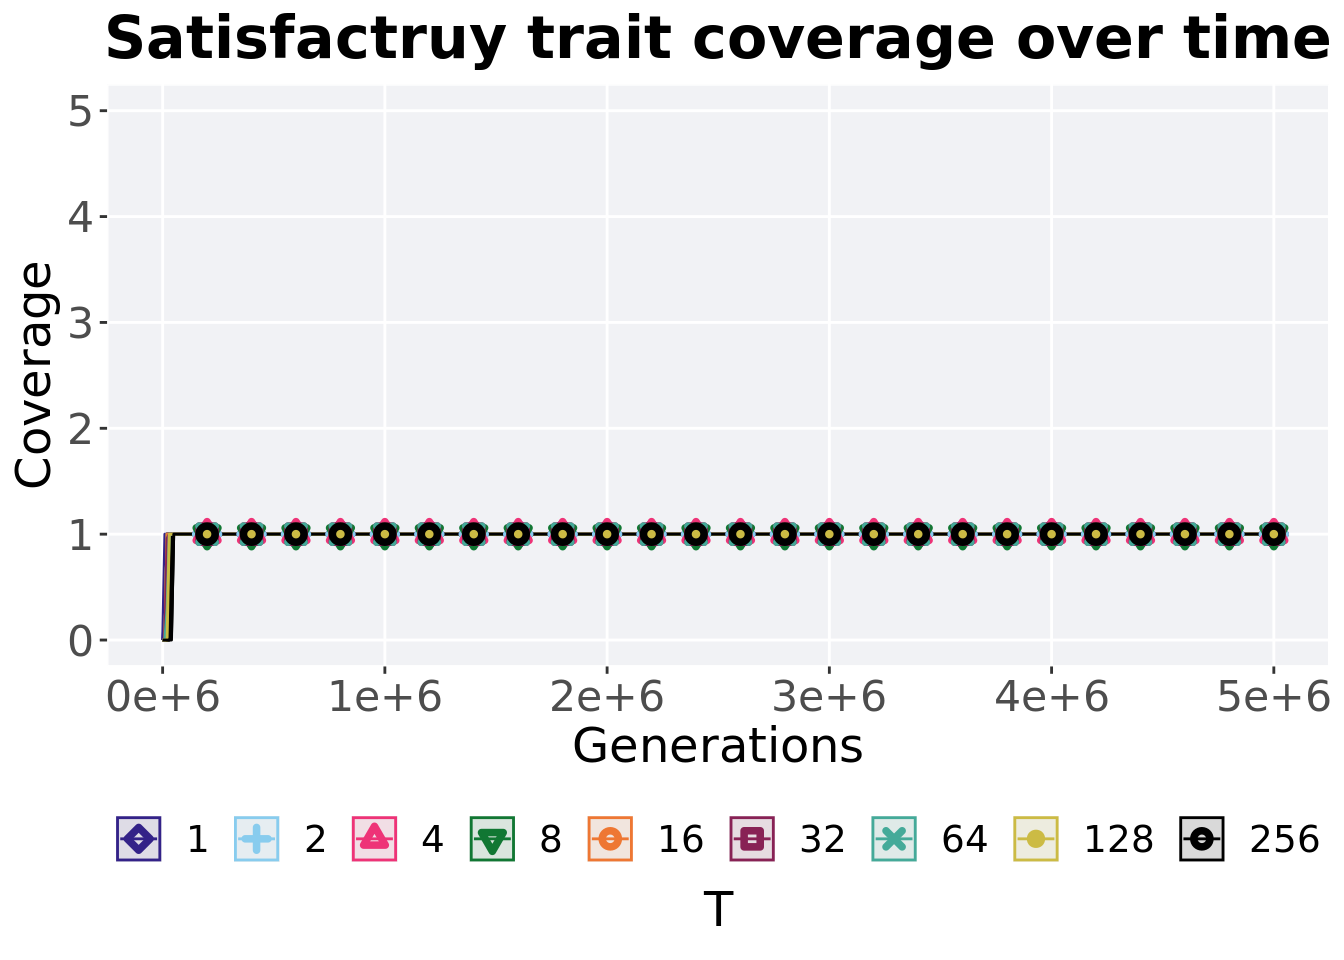
\includegraphics{demo_files/figure-latex/unnamed-chunk-89-1.pdf}

\hypertarget{end-of-50000-generations-6}{%
\subsubsection{End of 50,000 generations}\label{end-of-50000-generations-6}}

Activation gene coverage in the population at the end of 50,000 generations.

\begin{Shaded}
\begin{Highlighting}[]
\NormalTok{end =}\StringTok{ }\KeywordTok{filter}\NormalTok{(tru_end, diagnostic }\OperatorTok{==}\StringTok{ 'contradictory_objectives'}\NormalTok{)}
\NormalTok{plot =}\StringTok{ }\KeywordTok{ggplot}\NormalTok{(end, }\KeywordTok{aes}\NormalTok{(}\DataTypeTok{x =}\NormalTok{ T, }\DataTypeTok{y =}\NormalTok{ uni_str_pos, }\DataTypeTok{color =}\NormalTok{ T, }\DataTypeTok{fill =}\NormalTok{ T, }\DataTypeTok{shape =}\NormalTok{ T)) }\OperatorTok{+}
\StringTok{  }\KeywordTok{geom_flat_violin}\NormalTok{(}\DataTypeTok{position =} \KeywordTok{position_nudge}\NormalTok{(}\DataTypeTok{x =} \FloatTok{.2}\NormalTok{, }\DataTypeTok{y =} \DecValTok{0}\NormalTok{), }\DataTypeTok{scale =} \StringTok{'width'}\NormalTok{, }\DataTypeTok{alpha =} \FloatTok{0.2}\NormalTok{) }\OperatorTok{+}
\StringTok{  }\KeywordTok{geom_point}\NormalTok{(}\DataTypeTok{position =} \KeywordTok{position_jitter}\NormalTok{(}\DataTypeTok{width =} \FloatTok{.1}\NormalTok{), }\DataTypeTok{size =} \FloatTok{1.5}\NormalTok{, }\DataTypeTok{alpha =} \FloatTok{1.0}\NormalTok{) }\OperatorTok{+}
\StringTok{  }\KeywordTok{geom_boxplot}\NormalTok{(}\DataTypeTok{color =} \StringTok{'black'}\NormalTok{, }\DataTypeTok{width =} \FloatTok{.2}\NormalTok{, }\DataTypeTok{outlier.shape =} \OtherTok{NA}\NormalTok{, }\DataTypeTok{alpha =} \FloatTok{0.0}\NormalTok{) }\OperatorTok{+}
\StringTok{  }\KeywordTok{scale_y_continuous}\NormalTok{(}
    \DataTypeTok{name=}\StringTok{"Coverage"}\NormalTok{,}
    \DataTypeTok{limits=}\KeywordTok{c}\NormalTok{(}\DecValTok{0}\NormalTok{, }\DecValTok{5}\NormalTok{)}
\NormalTok{  ) }\OperatorTok{+}
\StringTok{  }\KeywordTok{scale_x_discrete}\NormalTok{(}
    \DataTypeTok{name=}\StringTok{"T"}
\NormalTok{  )}\OperatorTok{+}
\StringTok{  }\KeywordTok{scale_shape_manual}\NormalTok{(}\DataTypeTok{values=}\NormalTok{SHAPE)}\OperatorTok{+}
\StringTok{  }\KeywordTok{scale_colour_manual}\NormalTok{(}\DataTypeTok{values =}\NormalTok{ cb_palette) }\OperatorTok{+}
\StringTok{  }\KeywordTok{scale_fill_manual}\NormalTok{(}\DataTypeTok{values =}\NormalTok{ cb_palette) }\OperatorTok{+}
\StringTok{  }\NormalTok{p_theme}

\KeywordTok{plot_grid}\NormalTok{(}
\NormalTok{  plot }\OperatorTok{+}
\StringTok{    }\KeywordTok{ggtitle}\NormalTok{(}\StringTok{"Final activation gene coverage"}\NormalTok{) }\OperatorTok{+}
\StringTok{    }\KeywordTok{theme}\NormalTok{(}\DataTypeTok{legend.position=}\StringTok{"none"}\NormalTok{),}
\NormalTok{  legend,}
  \DataTypeTok{nrow=}\DecValTok{2}\NormalTok{,}
  \DataTypeTok{rel_heights =} \KeywordTok{c}\NormalTok{(}\DecValTok{2}\NormalTok{,.}\DecValTok{2}\NormalTok{),}
  \DataTypeTok{label_size =}\NormalTok{ TSIZE}
\NormalTok{)}
\end{Highlighting}
\end{Shaded}

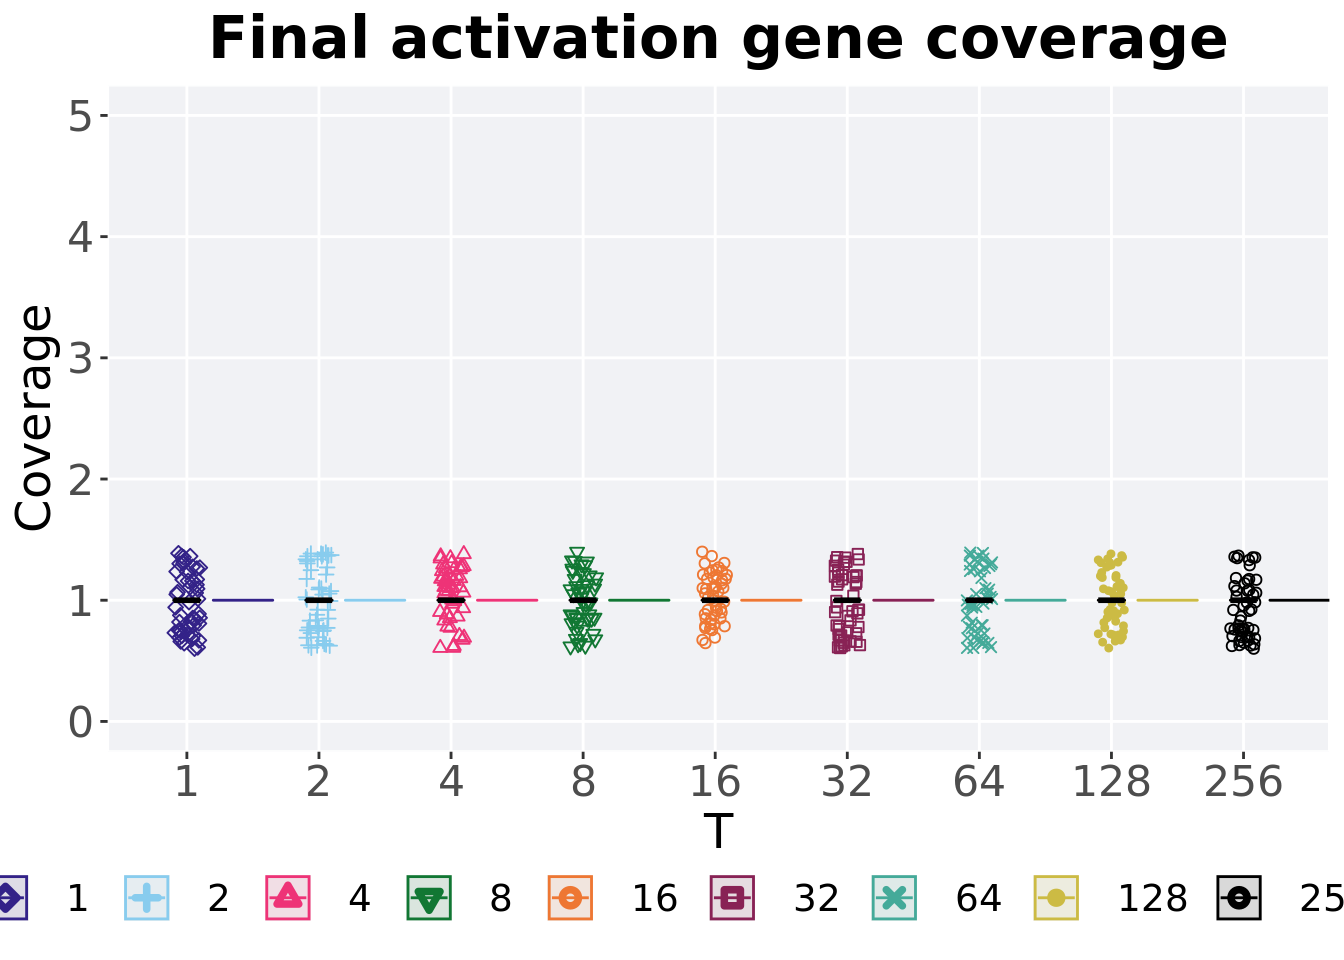
\includegraphics{demo_files/figure-latex/unnamed-chunk-90-1.pdf}

\hypertarget{stats-16}{%
\paragraph{Stats}\label{stats-16}}

Summary statistics for activation gene coverage in the population at the end of 50,000 generations.

\begin{Shaded}
\begin{Highlighting}[]
\KeywordTok{group_by}\NormalTok{(end, T) }\OperatorTok
\StringTok{  }\NormalTok{dplyr}\OperatorTok{::}\KeywordTok{summarise}\NormalTok{(}
    \DataTypeTok{count =} \KeywordTok{n}\NormalTok{(),}
    \DataTypeTok{na_cnt =} \KeywordTok{sum}\NormalTok{(}\KeywordTok{is.na}\NormalTok{(uni_str_pos)),}
    \DataTypeTok{min =} \KeywordTok{min}\NormalTok{(uni_str_pos, }\DataTypeTok{na.rm =} \OtherTok{TRUE}\NormalTok{),}
    \DataTypeTok{median =} \KeywordTok{median}\NormalTok{(uni_str_pos, }\DataTypeTok{na.rm =} \OtherTok{TRUE}\NormalTok{),}
    \DataTypeTok{mean =} \KeywordTok{mean}\NormalTok{(uni_str_pos, }\DataTypeTok{na.rm =} \OtherTok{TRUE}\NormalTok{),}
    \DataTypeTok{max =} \KeywordTok{max}\NormalTok{(uni_str_pos, }\DataTypeTok{na.rm =} \OtherTok{TRUE}\NormalTok{),}
    \DataTypeTok{IQR =} \KeywordTok{IQR}\NormalTok{(uni_str_pos, }\DataTypeTok{na.rm =} \OtherTok{TRUE}\NormalTok{)}
\NormalTok{  )}
\end{Highlighting}
\end{Shaded}

\begin{verbatim}
## # A tibble: 9 x 8
##   T     count na_cnt   min median  mean   max   IQR
##   <fct> <int>  <int> <int>  <dbl> <dbl> <int> <dbl>
## 1 1        50      0     1      1     1     1     0
## 2 2        50      0     1      1     1     1     0
## 3 4        50      0     1      1     1     1     0
## 4 8        50      0     1      1     1     1     0
## 5 16       50      0     1      1     1     1     0
## 6 32       50      0     1      1     1     1     0
## 7 64       50      0     1      1     1     1     0
## 8 128      50      0     1      1     1     1     0
## 9 256      50      0     1      1     1     1     0
\end{verbatim}

\hypertarget{multi-path-exploration-results-1}{%
\section{Multi-path exploration results}\label{multi-path-exploration-results-1}}

Here we present the results for \textbf{best performances} and \textbf{activation gene coverage} found by each genotypic fitness sharing sigma value replicate on the multi-path exploration diagnostic.
Best performance found refers to the largest average trait score found in a given population, while activation gene coverage refers to the count of unique activation genes in the population.
Note that both values fall between 0 and 100.

\hypertarget{performance-1}{%
\subsection{Performance}\label{performance-1}}

Here we analyze the performances for each parameter replicate on the multi-path exploration diagnostic.

\hypertarget{performance-over-time-4}{%
\subsubsection{Performance over time}\label{performance-over-time-4}}

Performance over time.

\begin{Shaded}
\begin{Highlighting}[]
\NormalTok{problem <-}\StringTok{ }\KeywordTok{filter}\NormalTok{(tru_ot, diagnostic }\OperatorTok{==}\StringTok{ 'multipath_exploration'}\NormalTok{)}
\NormalTok{lines =}\StringTok{ }\NormalTok{problem }\OperatorTok
\StringTok{        }\KeywordTok{group_by}\NormalTok{(T, gen) }\OperatorTok
\StringTok{          }\NormalTok{dplyr}\OperatorTok{::}\KeywordTok{summarise}\NormalTok{(}
            \DataTypeTok{min =} \KeywordTok{min}\NormalTok{(pop_fit_max),}
            \DataTypeTok{mean =} \KeywordTok{mean}\NormalTok{(pop_fit_max),}
            \DataTypeTok{max =} \KeywordTok{max}\NormalTok{(pop_fit_max)}
\NormalTok{          )}
\end{Highlighting}
\end{Shaded}

\begin{verbatim}
## `summarise()` has grouped output by 'T'. You can override using the `.groups`
## argument.
\end{verbatim}

\begin{Shaded}
\begin{Highlighting}[]
\NormalTok{points =}\StringTok{ }\KeywordTok{filter}\NormalTok{(lines, gen }\OperatorTok\StringTok{ }\DecValTok{2000} \OperatorTok{==}\StringTok{ }\DecValTok{0} \OperatorTok{&}\StringTok{ }\NormalTok{gen }\OperatorTok{!=}\StringTok{ }\DecValTok{0}\NormalTok{)}

\NormalTok{ot =}\StringTok{ }\KeywordTok{ggplot}\NormalTok{(lines, }\KeywordTok{aes}\NormalTok{(}\DataTypeTok{x=}\NormalTok{gen, }\DataTypeTok{y=}\NormalTok{mean }\OperatorTok{/}\StringTok{ }\NormalTok{TRAITS, }\DataTypeTok{group =}\NormalTok{ T, }\DataTypeTok{fill =}\NormalTok{ T, }\DataTypeTok{color =}\NormalTok{ T, }\DataTypeTok{shape =}\NormalTok{ T)) }\OperatorTok{+}
\StringTok{  }\KeywordTok{geom_ribbon}\NormalTok{(}\KeywordTok{aes}\NormalTok{(}\DataTypeTok{ymin =}\NormalTok{ min }\OperatorTok{/}\StringTok{ }\NormalTok{TRAITS, }\DataTypeTok{ymax =}\NormalTok{ max }\OperatorTok{/}\StringTok{ }\NormalTok{TRAITS), }\DataTypeTok{alpha =} \FloatTok{0.1}\NormalTok{) }\OperatorTok{+}
\StringTok{  }\KeywordTok{geom_line}\NormalTok{(}\DataTypeTok{size =} \FloatTok{0.5}\NormalTok{) }\OperatorTok{+}
\StringTok{  }\KeywordTok{geom_point}\NormalTok{(}\DataTypeTok{data =}\NormalTok{ points, }\DataTypeTok{size =} \FloatTok{1.5}\NormalTok{, }\DataTypeTok{stroke =} \FloatTok{2.0}\NormalTok{, }\DataTypeTok{alpha =} \FloatTok{1.0}\NormalTok{) }\OperatorTok{+}
\StringTok{  }\KeywordTok{scale_y_continuous}\NormalTok{(}
    \DataTypeTok{name=}\StringTok{"Average trait score"}\NormalTok{,}
    \DataTypeTok{limits=}\KeywordTok{c}\NormalTok{(}\OperatorTok{-}\DecValTok{1}\NormalTok{, }\DecValTok{101}\NormalTok{),}
    \DataTypeTok{breaks=}\KeywordTok{seq}\NormalTok{(}\DecValTok{0}\NormalTok{,}\DecValTok{100}\NormalTok{, }\DecValTok{20}\NormalTok{),}
    \DataTypeTok{labels=}\KeywordTok{c}\NormalTok{(}\StringTok{"0"}\NormalTok{, }\StringTok{"20"}\NormalTok{, }\StringTok{"40"}\NormalTok{, }\StringTok{"60"}\NormalTok{, }\StringTok{"80"}\NormalTok{, }\StringTok{"100"}\NormalTok{)}
\NormalTok{  ) }\OperatorTok{+}
\StringTok{  }\KeywordTok{scale_x_continuous}\NormalTok{(}
    \DataTypeTok{name=}\StringTok{"Generations"}\NormalTok{,}
    \DataTypeTok{limits=}\KeywordTok{c}\NormalTok{(}\DecValTok{0}\NormalTok{, }\DecValTok{50000}\NormalTok{),}
    \DataTypeTok{breaks=}\KeywordTok{c}\NormalTok{(}\DecValTok{0}\NormalTok{, }\DecValTok{10000}\NormalTok{, }\DecValTok{20000}\NormalTok{, }\DecValTok{30000}\NormalTok{, }\DecValTok{40000}\NormalTok{, }\DecValTok{50000}\NormalTok{),}
    \DataTypeTok{labels=}\KeywordTok{c}\NormalTok{(}\StringTok{"0e+6"}\NormalTok{, }\StringTok{"1e+6"}\NormalTok{, }\StringTok{"2e+6"}\NormalTok{, }\StringTok{"3e+6"}\NormalTok{, }\StringTok{"4e+6"}\NormalTok{, }\StringTok{"5e+6"}\NormalTok{)}

\NormalTok{  ) }\OperatorTok{+}
\StringTok{  }\KeywordTok{scale_shape_manual}\NormalTok{(}\DataTypeTok{values=}\NormalTok{SHAPE)}\OperatorTok{+}
\StringTok{  }\KeywordTok{scale_colour_manual}\NormalTok{(}\DataTypeTok{values =}\NormalTok{ cb_palette) }\OperatorTok{+}
\StringTok{  }\KeywordTok{scale_fill_manual}\NormalTok{(}\DataTypeTok{values =}\NormalTok{ cb_palette) }\OperatorTok{+}
\StringTok{  }\KeywordTok{ggtitle}\NormalTok{(}\StringTok{"Best performance over time"}\NormalTok{) }\OperatorTok{+}
\StringTok{  }\NormalTok{p_theme}\OperatorTok{+}
\StringTok{    }\KeywordTok{guides}\NormalTok{(}
    \DataTypeTok{shape=}\KeywordTok{guide_legend}\NormalTok{(}\DataTypeTok{nrow=}\DecValTok{1}\NormalTok{, }\DataTypeTok{title.position =} \StringTok{"bottom"}\NormalTok{),}
    \DataTypeTok{color=}\KeywordTok{guide_legend}\NormalTok{(}\DataTypeTok{nrow=}\DecValTok{1}\NormalTok{, }\DataTypeTok{title.position =} \StringTok{"bottom"}\NormalTok{),}
    \DataTypeTok{fill=}\KeywordTok{guide_legend}\NormalTok{(}\DataTypeTok{nrow=}\DecValTok{1}\NormalTok{, }\DataTypeTok{title.position =} \StringTok{"bottom"}\NormalTok{)}
\NormalTok{  ) }\OperatorTok{+}
\StringTok{  }\KeywordTok{theme}\NormalTok{(}
    \DataTypeTok{legend.position =} \StringTok{"bottom"}\NormalTok{,}
    \DataTypeTok{legend.box=}\StringTok{"verticle"}\NormalTok{,}
    \DataTypeTok{legend.justification=}\StringTok{"center"}\NormalTok{,}
    \DataTypeTok{legend.title.align=}\FloatTok{0.5}
\NormalTok{  )}

\NormalTok{ot}
\end{Highlighting}
\end{Shaded}

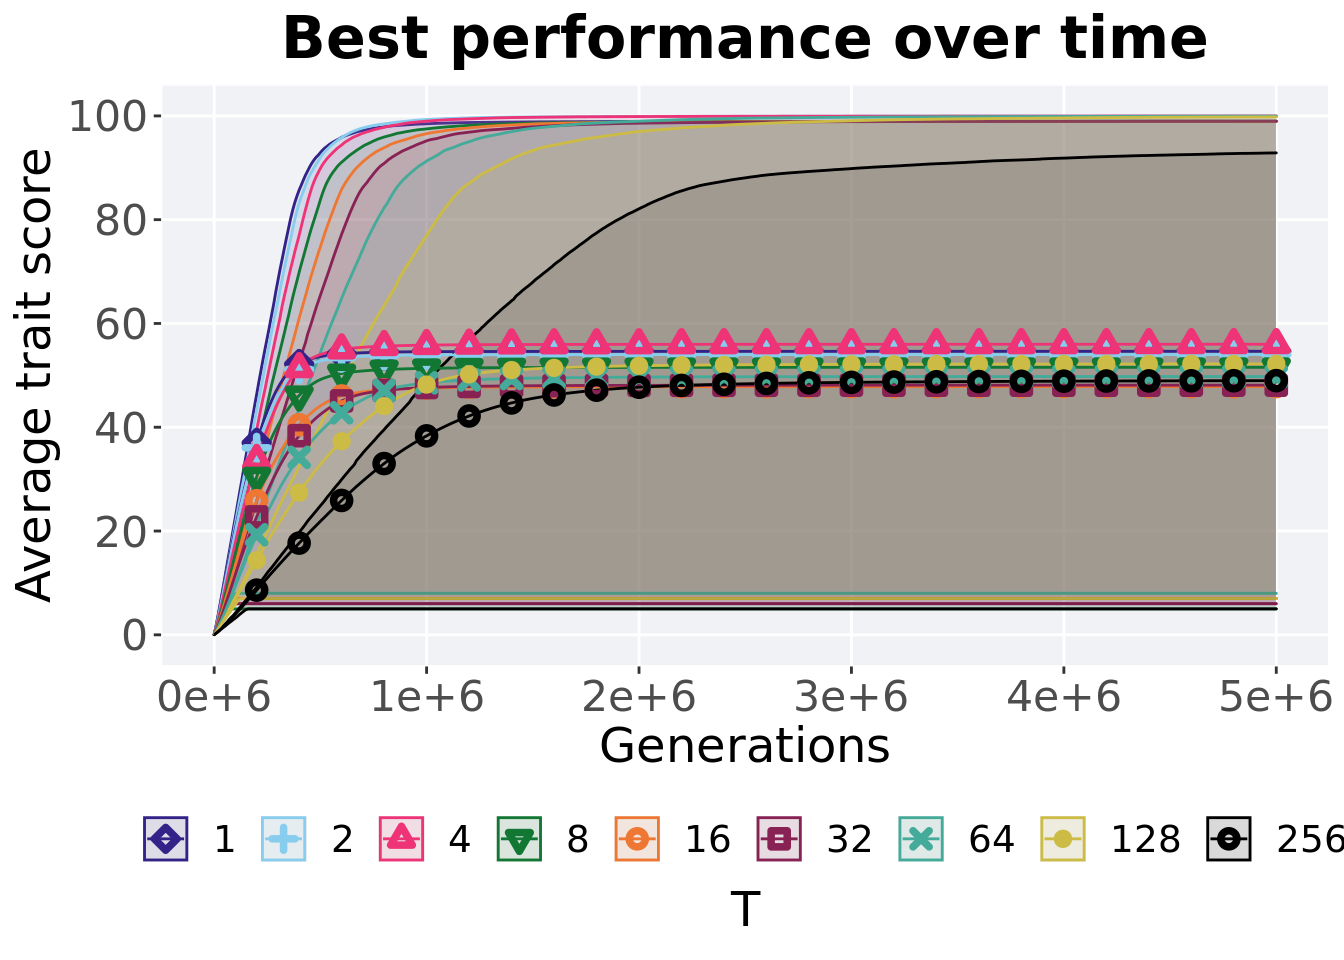
\includegraphics{demo_files/figure-latex/unnamed-chunk-92-1.pdf}

\hypertarget{best-performance-throughout-3}{%
\subsubsection{Best performance throughout}\label{best-performance-throughout-3}}

Here we plot the performance of the best performing solution found throughout 50,000 generations.

\begin{Shaded}
\begin{Highlighting}[]
\NormalTok{best =}\StringTok{ }\KeywordTok{filter}\NormalTok{(tru_best, col }\OperatorTok{==}\StringTok{ 'pop_fit_max'} \OperatorTok{&}\StringTok{ }\NormalTok{diagnostic }\OperatorTok{==}\StringTok{ 'multipath_exploration'}\NormalTok{)}

\NormalTok{plot =}\StringTok{ }\KeywordTok{ggplot}\NormalTok{(best, }\KeywordTok{aes}\NormalTok{(}\DataTypeTok{x =}\NormalTok{ T, }\DataTypeTok{y =}\NormalTok{ val }\OperatorTok{/}\StringTok{ }\NormalTok{TRAITS, }\DataTypeTok{color =}\NormalTok{ T, }\DataTypeTok{fill =}\NormalTok{ T, }\DataTypeTok{shape =}\NormalTok{ T)) }\OperatorTok{+}
\StringTok{  }\KeywordTok{geom_flat_violin}\NormalTok{(}\DataTypeTok{position =} \KeywordTok{position_nudge}\NormalTok{(}\DataTypeTok{x =} \FloatTok{.2}\NormalTok{, }\DataTypeTok{y =} \DecValTok{0}\NormalTok{), }\DataTypeTok{scale =} \StringTok{'width'}\NormalTok{, }\DataTypeTok{alpha =} \FloatTok{0.2}\NormalTok{) }\OperatorTok{+}
\StringTok{  }\KeywordTok{geom_point}\NormalTok{(}\DataTypeTok{position =} \KeywordTok{position_jitter}\NormalTok{(}\DataTypeTok{width =} \FloatTok{.1}\NormalTok{), }\DataTypeTok{size =} \FloatTok{1.5}\NormalTok{, }\DataTypeTok{alpha =} \FloatTok{1.0}\NormalTok{) }\OperatorTok{+}
\StringTok{  }\KeywordTok{geom_boxplot}\NormalTok{(}\DataTypeTok{color =} \StringTok{'black'}\NormalTok{, }\DataTypeTok{width =} \FloatTok{.2}\NormalTok{, }\DataTypeTok{outlier.shape =} \OtherTok{NA}\NormalTok{, }\DataTypeTok{alpha =} \FloatTok{0.0}\NormalTok{) }\OperatorTok{+}
\StringTok{  }\KeywordTok{scale_y_continuous}\NormalTok{(}
    \DataTypeTok{name=}\StringTok{"Average trait score"}\NormalTok{,}
    \DataTypeTok{limits=}\KeywordTok{c}\NormalTok{(}\OperatorTok{-}\DecValTok{1}\NormalTok{, }\DecValTok{101}\NormalTok{),}
    \DataTypeTok{breaks=}\KeywordTok{seq}\NormalTok{(}\DecValTok{0}\NormalTok{,}\DecValTok{100}\NormalTok{, }\DecValTok{20}\NormalTok{),}
    \DataTypeTok{labels=}\KeywordTok{c}\NormalTok{(}\StringTok{"0"}\NormalTok{, }\StringTok{"20"}\NormalTok{, }\StringTok{"40"}\NormalTok{, }\StringTok{"60"}\NormalTok{, }\StringTok{"80"}\NormalTok{, }\StringTok{"100"}\NormalTok{)}
\NormalTok{  ) }\OperatorTok{+}
\StringTok{  }\KeywordTok{scale_x_discrete}\NormalTok{(}
    \DataTypeTok{name=}\StringTok{"T"}
\NormalTok{  )}\OperatorTok{+}
\StringTok{  }\KeywordTok{scale_shape_manual}\NormalTok{(}\DataTypeTok{values=}\NormalTok{SHAPE)}\OperatorTok{+}
\StringTok{  }\KeywordTok{scale_colour_manual}\NormalTok{(}\DataTypeTok{values =}\NormalTok{ cb_palette) }\OperatorTok{+}
\StringTok{  }\KeywordTok{scale_fill_manual}\NormalTok{(}\DataTypeTok{values =}\NormalTok{ cb_palette) }\OperatorTok{+}
\StringTok{  }\NormalTok{p_theme}

\KeywordTok{plot_grid}\NormalTok{(}
\NormalTok{  plot }\OperatorTok{+}
\StringTok{    }\KeywordTok{ggtitle}\NormalTok{(}\StringTok{"Best performance throughout"}\NormalTok{) }\OperatorTok{+}
\StringTok{    }\KeywordTok{theme}\NormalTok{(}\DataTypeTok{legend.position=}\StringTok{"none"}\NormalTok{),}
\NormalTok{  legend,}
  \DataTypeTok{nrow=}\DecValTok{2}\NormalTok{,}
  \DataTypeTok{rel_heights =} \KeywordTok{c}\NormalTok{(}\DecValTok{2}\NormalTok{,.}\DecValTok{3}\NormalTok{),}
  \DataTypeTok{label_size =}\NormalTok{ TSIZE}
\NormalTok{)}
\end{Highlighting}
\end{Shaded}

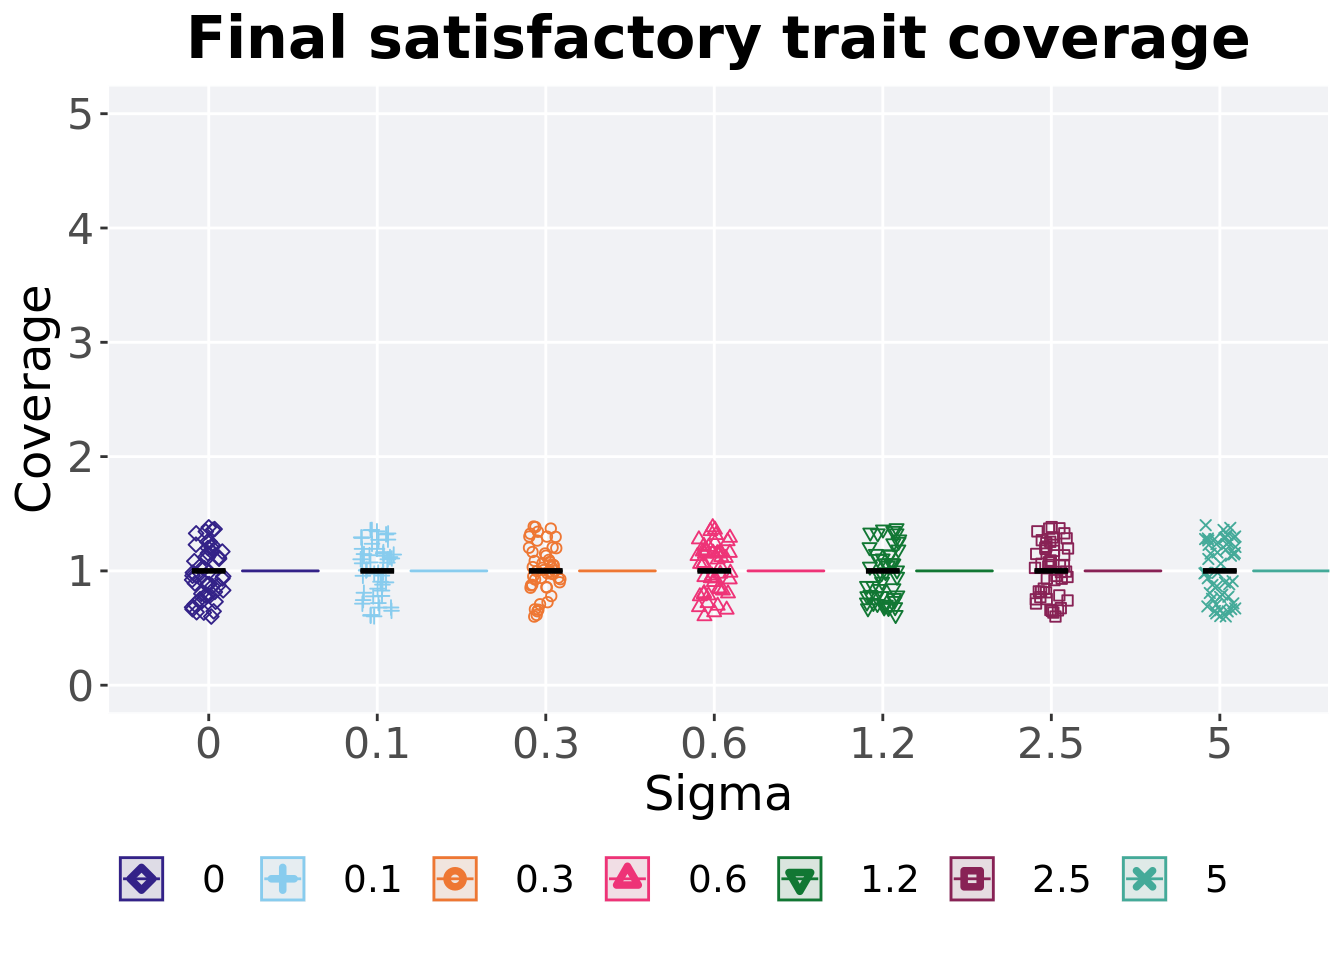
\includegraphics{demo_files/figure-latex/unnamed-chunk-94-1.pdf}

\hypertarget{stats-17}{%
\paragraph{Stats}\label{stats-17}}

Summary statistics for the performance of the best performing solution found throughout 50,000 generations.

\begin{Shaded}
\begin{Highlighting}[]
\KeywordTok{group_by}\NormalTok{(best, T) }\OperatorTok
\StringTok{  }\NormalTok{dplyr}\OperatorTok{::}\KeywordTok{summarise}\NormalTok{(}
    \DataTypeTok{count =} \KeywordTok{n}\NormalTok{(),}
    \DataTypeTok{na_cnt =} \KeywordTok{sum}\NormalTok{(}\KeywordTok{is.na}\NormalTok{(val)),}
    \DataTypeTok{min =} \KeywordTok{min}\NormalTok{(val }\OperatorTok{/}\StringTok{ }\NormalTok{TRAITS, }\DataTypeTok{na.rm =} \OtherTok{TRUE}\NormalTok{),}
    \DataTypeTok{median =} \KeywordTok{median}\NormalTok{(val }\OperatorTok{/}\StringTok{ }\NormalTok{TRAITS, }\DataTypeTok{na.rm =} \OtherTok{TRUE}\NormalTok{),}
    \DataTypeTok{mean =} \KeywordTok{mean}\NormalTok{(val }\OperatorTok{/}\StringTok{ }\NormalTok{TRAITS, }\DataTypeTok{na.rm =} \OtherTok{TRUE}\NormalTok{),}
    \DataTypeTok{max =} \KeywordTok{max}\NormalTok{(val }\OperatorTok{/}\StringTok{ }\NormalTok{TRAITS, }\DataTypeTok{na.rm =} \OtherTok{TRUE}\NormalTok{),}
    \DataTypeTok{IQR =} \KeywordTok{IQR}\NormalTok{(val }\OperatorTok{/}\StringTok{ }\NormalTok{TRAITS, }\DataTypeTok{na.rm =} \OtherTok{TRUE}\NormalTok{)}
\NormalTok{  )}
\end{Highlighting}
\end{Shaded}

\begin{verbatim}
## # A tibble: 9 x 8
##   T     count na_cnt   min median  mean   max   IQR
##   <fct> <int>  <int> <dbl>  <dbl> <dbl> <dbl> <dbl>
## 1 1        50      0  7      55.0  54.6  99.0  44.0
## 2 2        50      0  8      50.0  54.0 100.   50.2
## 3 4        50      0  6      57.5  56.0 100.   47.5
## 4 8        50      0  5      49.0  51.6  99.0  38.5
## 5 16       50      0  7      41.0  47.8  99.0  38.2
## 6 32       50      0  6      44.5  48.1  99.0  38.5
## 7 64       50      0  8      46.0  49.8  99.9  38.0
## 8 128      50      0  7.00   48.5  52.2  99.8  43.5
## 9 256      50      0  5      51.5  49.0  92.9  29.4
\end{verbatim}

Kruskal--Wallis test provides evidence of no statistical differences among the best performing solution found throughout 50,000 generations.

\begin{Shaded}
\begin{Highlighting}[]
\KeywordTok{kruskal.test}\NormalTok{(val }\OperatorTok{~}\StringTok{ }\NormalTok{T,}\DataTypeTok{data =}\NormalTok{ best)}
\end{Highlighting}
\end{Shaded}

\begin{verbatim}
## 
##  Kruskal-Wallis rank sum test
## 
## data:  val by T
## Kruskal-Wallis chi-squared = 5.0721, df = 8, p-value = 0.7498
\end{verbatim}

\hypertarget{end-of-50000-generations-7}{%
\subsubsection{End of 50,000 generations}\label{end-of-50000-generations-7}}

Best performance in the population at the end of 50,000 generations.

\begin{Shaded}
\begin{Highlighting}[]
\NormalTok{end =}\StringTok{ }\KeywordTok{filter}\NormalTok{(tru_end, diagnostic }\OperatorTok{==}\StringTok{ 'multipath_exploration'}\NormalTok{)}
\NormalTok{plot =}\StringTok{ }\KeywordTok{ggplot}\NormalTok{(end, }\KeywordTok{aes}\NormalTok{(}\DataTypeTok{x =}\NormalTok{ T, }\DataTypeTok{y =}\NormalTok{ pop_fit_max }\OperatorTok{/}\StringTok{ }\NormalTok{TRAITS, }\DataTypeTok{color =}\NormalTok{ T, }\DataTypeTok{fill =}\NormalTok{ T, }\DataTypeTok{shape =}\NormalTok{ T)) }\OperatorTok{+}
\StringTok{  }\KeywordTok{geom_flat_violin}\NormalTok{(}\DataTypeTok{position =} \KeywordTok{position_nudge}\NormalTok{(}\DataTypeTok{x =} \FloatTok{.2}\NormalTok{, }\DataTypeTok{y =} \DecValTok{0}\NormalTok{), }\DataTypeTok{scale =} \StringTok{'width'}\NormalTok{, }\DataTypeTok{alpha =} \FloatTok{0.2}\NormalTok{) }\OperatorTok{+}
\StringTok{  }\KeywordTok{geom_point}\NormalTok{(}\DataTypeTok{position =} \KeywordTok{position_jitter}\NormalTok{(}\DataTypeTok{width =} \FloatTok{.1}\NormalTok{), }\DataTypeTok{size =} \FloatTok{1.5}\NormalTok{, }\DataTypeTok{alpha =} \FloatTok{1.0}\NormalTok{) }\OperatorTok{+}
\StringTok{  }\KeywordTok{geom_boxplot}\NormalTok{(}\DataTypeTok{color =} \StringTok{'black'}\NormalTok{, }\DataTypeTok{width =} \FloatTok{.2}\NormalTok{, }\DataTypeTok{outlier.shape =} \OtherTok{NA}\NormalTok{, }\DataTypeTok{alpha =} \FloatTok{0.0}\NormalTok{) }\OperatorTok{+}
\StringTok{  }\KeywordTok{scale_y_continuous}\NormalTok{(}
    \DataTypeTok{name=}\StringTok{"Average trait score"}\NormalTok{,}
    \DataTypeTok{limits=}\KeywordTok{c}\NormalTok{(}\OperatorTok{-}\DecValTok{1}\NormalTok{, }\DecValTok{101}\NormalTok{),}
    \DataTypeTok{breaks=}\KeywordTok{seq}\NormalTok{(}\DecValTok{0}\NormalTok{,}\DecValTok{100}\NormalTok{, }\DecValTok{20}\NormalTok{),}
    \DataTypeTok{labels=}\KeywordTok{c}\NormalTok{(}\StringTok{"0"}\NormalTok{, }\StringTok{"20"}\NormalTok{, }\StringTok{"40"}\NormalTok{, }\StringTok{"60"}\NormalTok{, }\StringTok{"80"}\NormalTok{, }\StringTok{"100"}\NormalTok{)}
\NormalTok{  ) }\OperatorTok{+}
\StringTok{  }\KeywordTok{scale_x_discrete}\NormalTok{(}
    \DataTypeTok{name=}\StringTok{"T"}
\NormalTok{  )}\OperatorTok{+}
\StringTok{  }\KeywordTok{scale_shape_manual}\NormalTok{(}\DataTypeTok{values=}\NormalTok{SHAPE)}\OperatorTok{+}
\StringTok{  }\KeywordTok{scale_colour_manual}\NormalTok{(}\DataTypeTok{values =}\NormalTok{ cb_palette) }\OperatorTok{+}
\StringTok{  }\KeywordTok{scale_fill_manual}\NormalTok{(}\DataTypeTok{values =}\NormalTok{ cb_palette) }\OperatorTok{+}
\StringTok{  }\NormalTok{p_theme}

\KeywordTok{plot_grid}\NormalTok{(}
\NormalTok{  plot }\OperatorTok{+}
\StringTok{    }\KeywordTok{ggtitle}\NormalTok{(}\StringTok{"Final performance"}\NormalTok{) }\OperatorTok{+}
\StringTok{    }\KeywordTok{theme}\NormalTok{(}\DataTypeTok{legend.position=}\StringTok{"none"}\NormalTok{),}
\NormalTok{  legend,}
  \DataTypeTok{nrow=}\DecValTok{2}\NormalTok{,}
  \DataTypeTok{rel_heights =} \KeywordTok{c}\NormalTok{(}\DecValTok{2}\NormalTok{,.}\DecValTok{3}\NormalTok{),}
  \DataTypeTok{label_size =}\NormalTok{ TSIZE}
\NormalTok{)}
\end{Highlighting}
\end{Shaded}

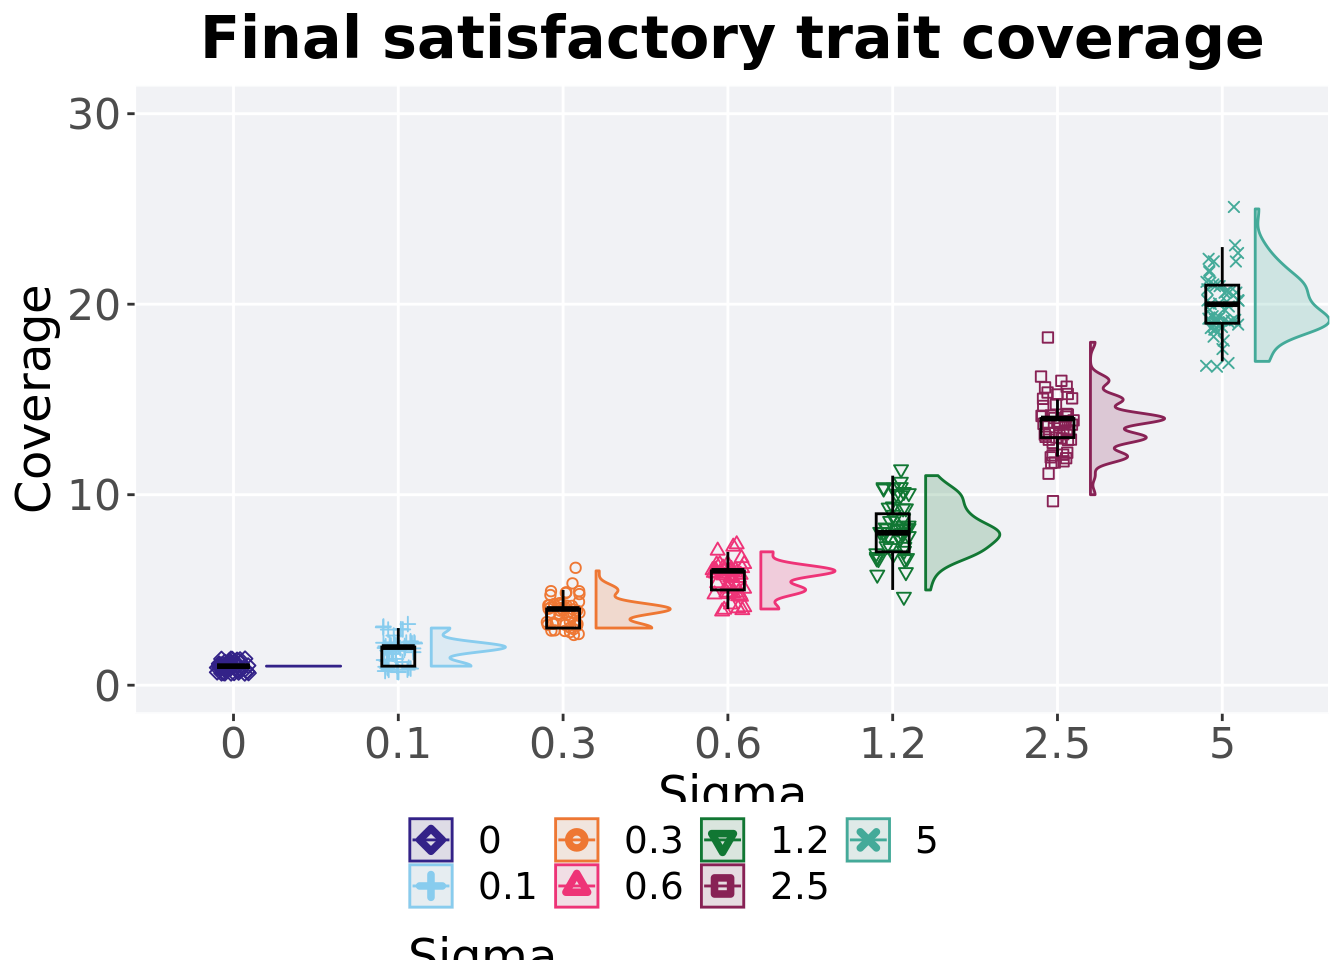
\includegraphics{demo_files/figure-latex/unnamed-chunk-97-1.pdf}

\hypertarget{stats-18}{%
\paragraph{Stats}\label{stats-18}}

Summary statistics for the best performance in the population at the end of 50,000 generations.

\begin{Shaded}
\begin{Highlighting}[]
\KeywordTok{group_by}\NormalTok{(end, T) }\OperatorTok
\StringTok{  }\NormalTok{dplyr}\OperatorTok{::}\KeywordTok{summarise}\NormalTok{(}
    \DataTypeTok{count =} \KeywordTok{n}\NormalTok{(),}
    \DataTypeTok{na_cnt =} \KeywordTok{sum}\NormalTok{(}\KeywordTok{is.na}\NormalTok{(pop_fit_max }\OperatorTok{/}\StringTok{ }\NormalTok{TRAITS)),}
    \DataTypeTok{min =} \KeywordTok{min}\NormalTok{(pop_fit_max }\OperatorTok{/}\StringTok{ }\NormalTok{TRAITS, }\DataTypeTok{na.rm =} \OtherTok{TRUE}\NormalTok{),}
    \DataTypeTok{median =} \KeywordTok{median}\NormalTok{(pop_fit_max }\OperatorTok{/}\StringTok{ }\NormalTok{TRAITS, }\DataTypeTok{na.rm =} \OtherTok{TRUE}\NormalTok{),}
    \DataTypeTok{mean =} \KeywordTok{mean}\NormalTok{(pop_fit_max }\OperatorTok{/}\StringTok{ }\NormalTok{TRAITS, }\DataTypeTok{na.rm =} \OtherTok{TRUE}\NormalTok{),}
    \DataTypeTok{max =} \KeywordTok{max}\NormalTok{(pop_fit_max }\OperatorTok{/}\StringTok{ }\NormalTok{TRAITS, }\DataTypeTok{na.rm =} \OtherTok{TRUE}\NormalTok{),}
    \DataTypeTok{IQR =} \KeywordTok{IQR}\NormalTok{(pop_fit_max }\OperatorTok{/}\StringTok{ }\NormalTok{TRAITS, }\DataTypeTok{na.rm =} \OtherTok{TRUE}\NormalTok{)}
\NormalTok{  )}
\end{Highlighting}
\end{Shaded}

\begin{verbatim}
## # A tibble: 9 x 8
##   T     count na_cnt   min median  mean   max   IQR
##   <fct> <int>  <int> <dbl>  <dbl> <dbl> <dbl> <dbl>
## 1 1        50      0  7      55.0  54.6  99.0  44.0
## 2 2        50      0  8      50.0  54.0 100.   50.2
## 3 4        50      0  6      57.5  56.0 100.   47.5
## 4 8        50      0  5      49.0  51.6  99.0  38.5
## 5 16       50      0  7      41.0  47.8  99.0  38.2
## 6 32       50      0  6      44.5  48.1  99.0  38.5
## 7 64       50      0  8      46.0  49.8  99.9  38.0
## 8 128      50      0  7.00   48.5  52.2  99.8  43.5
## 9 256      50      0  5      51.5  49.0  92.9  29.4
\end{verbatim}

Kruskal--Wallis test provides evidence of statistical differences among best performance in the population at the end of 50,000 generations.

\begin{Shaded}
\begin{Highlighting}[]
\KeywordTok{kruskal.test}\NormalTok{(pop_fit_max }\OperatorTok{~}\StringTok{ }\NormalTok{T, }\DataTypeTok{data =}\NormalTok{ end)}
\end{Highlighting}
\end{Shaded}

\begin{verbatim}
## 
##  Kruskal-Wallis rank sum test
## 
## data:  pop_fit_max by T
## Kruskal-Wallis chi-squared = 5.0721, df = 8, p-value = 0.7498
\end{verbatim}

Results for post-hoc Wilcoxon rank-sum test with a Bonferroni correction on the best performance in the population at the end of 50,000 generations.

\begin{Shaded}
\begin{Highlighting}[]
\KeywordTok{pairwise.wilcox.test}\NormalTok{(}\DataTypeTok{x =}\NormalTok{ end}\OperatorTok{$}\NormalTok{pop_fit_max, }\DataTypeTok{g =}\NormalTok{ end}\OperatorTok{$}\NormalTok{T , }\DataTypeTok{p.adjust.method =} \StringTok{"bonferroni"}\NormalTok{,}
                     \DataTypeTok{paired =} \OtherTok{FALSE}\NormalTok{, }\DataTypeTok{conf.int =} \OtherTok{FALSE}\NormalTok{, }\DataTypeTok{alternative =} \StringTok{'l'}\NormalTok{)}
\end{Highlighting}
\end{Shaded}

\begin{verbatim}
## 
##  Pairwise comparisons using Wilcoxon rank sum test with continuity correction 
## 
## data:  end$pop_fit_max and end$T 
## 
##     1 2 4 8 16 32 64 128
## 2   1 - - - -  -  -  -  
## 4   1 1 - - -  -  -  -  
## 8   1 1 1 - -  -  -  -  
## 16  1 1 1 1 -  -  -  -  
## 32  1 1 1 1 1  -  -  -  
## 64  1 1 1 1 1  1  -  -  
## 128 1 1 1 1 1  1  1  -  
## 256 1 1 1 1 1  1  1  1  
## 
## P value adjustment method: bonferroni
\end{verbatim}

\hypertarget{activation-gene-coverage-3}{%
\subsection{Activation gene coverage}\label{activation-gene-coverage-3}}

Here we analyze the activation gene coverage for each parameter replicate on the multi-path exploration diagnostic.

\hypertarget{coverage-over-time-4}{%
\subsubsection{Coverage over time}\label{coverage-over-time-4}}

Activation gene coverage over time.

\begin{Shaded}
\begin{Highlighting}[]
\NormalTok{problem <-}\StringTok{ }\KeywordTok{filter}\NormalTok{(tru_ot, diagnostic }\OperatorTok{==}\StringTok{ 'multipath_exploration'}\NormalTok{)}
\NormalTok{lines =}\StringTok{ }\NormalTok{problem }\OperatorTok
\StringTok{        }\KeywordTok{group_by}\NormalTok{(T, gen) }\OperatorTok
\StringTok{          }\NormalTok{dplyr}\OperatorTok{::}\KeywordTok{summarise}\NormalTok{(}
            \DataTypeTok{min =} \KeywordTok{min}\NormalTok{(uni_str_pos),}
            \DataTypeTok{mean =} \KeywordTok{mean}\NormalTok{(uni_str_pos),}
            \DataTypeTok{max =} \KeywordTok{max}\NormalTok{(uni_str_pos)}
\NormalTok{          )}
\end{Highlighting}
\end{Shaded}

\begin{verbatim}
## `summarise()` has grouped output by 'T'. You can override using the `.groups`
## argument.
\end{verbatim}

\begin{Shaded}
\begin{Highlighting}[]
\NormalTok{points =}\StringTok{ }\KeywordTok{filter}\NormalTok{(lines, gen }\OperatorTok\StringTok{ }\DecValTok{2000} \OperatorTok{==}\StringTok{ }\DecValTok{0} \OperatorTok{&}\StringTok{ }\NormalTok{gen }\OperatorTok{!=}\StringTok{ }\DecValTok{0}\NormalTok{)}

\NormalTok{ot =}\StringTok{ }\KeywordTok{ggplot}\NormalTok{(lines, }\KeywordTok{aes}\NormalTok{(}\DataTypeTok{x=}\NormalTok{gen, }\DataTypeTok{y=}\NormalTok{mean, }\DataTypeTok{group =}\NormalTok{ T, }\DataTypeTok{fill =}\NormalTok{T, }\DataTypeTok{color =}\NormalTok{ T, }\DataTypeTok{shape =}\NormalTok{ T)) }\OperatorTok{+}
\StringTok{  }\KeywordTok{geom_ribbon}\NormalTok{(}\KeywordTok{aes}\NormalTok{(}\DataTypeTok{ymin =}\NormalTok{ min, }\DataTypeTok{ymax =}\NormalTok{ max), }\DataTypeTok{alpha =} \FloatTok{0.1}\NormalTok{) }\OperatorTok{+}
\StringTok{  }\KeywordTok{geom_line}\NormalTok{(}\DataTypeTok{size =} \FloatTok{0.5}\NormalTok{) }\OperatorTok{+}
\StringTok{  }\KeywordTok{geom_point}\NormalTok{(}\DataTypeTok{data =}\NormalTok{ points, }\DataTypeTok{size =} \FloatTok{1.5}\NormalTok{, }\DataTypeTok{stroke =} \FloatTok{2.0}\NormalTok{, }\DataTypeTok{alpha =} \FloatTok{1.0}\NormalTok{) }\OperatorTok{+}
\StringTok{  }\KeywordTok{scale_y_continuous}\NormalTok{(}
    \DataTypeTok{name=}\StringTok{"Coverage"}\NormalTok{,}
    \DataTypeTok{limits=}\KeywordTok{c}\NormalTok{(}\OperatorTok{-}\DecValTok{1}\NormalTok{, }\DecValTok{101}\NormalTok{),}
    \DataTypeTok{breaks=}\KeywordTok{seq}\NormalTok{(}\DecValTok{0}\NormalTok{,}\DecValTok{100}\NormalTok{, }\DecValTok{20}\NormalTok{),}
    \DataTypeTok{labels=}\KeywordTok{c}\NormalTok{(}\StringTok{"0"}\NormalTok{, }\StringTok{"20"}\NormalTok{, }\StringTok{"40"}\NormalTok{, }\StringTok{"60"}\NormalTok{, }\StringTok{"80"}\NormalTok{, }\StringTok{"100"}\NormalTok{)}
\NormalTok{  ) }\OperatorTok{+}
\StringTok{  }\KeywordTok{scale_x_continuous}\NormalTok{(}
    \DataTypeTok{name=}\StringTok{"Generations"}\NormalTok{,}
    \DataTypeTok{limits=}\KeywordTok{c}\NormalTok{(}\DecValTok{0}\NormalTok{, }\DecValTok{50000}\NormalTok{),}
    \DataTypeTok{breaks=}\KeywordTok{c}\NormalTok{(}\DecValTok{0}\NormalTok{, }\DecValTok{10000}\NormalTok{, }\DecValTok{20000}\NormalTok{, }\DecValTok{30000}\NormalTok{, }\DecValTok{40000}\NormalTok{, }\DecValTok{50000}\NormalTok{),}
    \DataTypeTok{labels=}\KeywordTok{c}\NormalTok{(}\StringTok{"0e+6"}\NormalTok{, }\StringTok{"1e+6"}\NormalTok{, }\StringTok{"2e+6"}\NormalTok{, }\StringTok{"3e+6"}\NormalTok{, }\StringTok{"4e+6"}\NormalTok{, }\StringTok{"5e+6"}\NormalTok{)}

\NormalTok{  ) }\OperatorTok{+}
\StringTok{  }\KeywordTok{scale_shape_manual}\NormalTok{(}\DataTypeTok{values=}\NormalTok{SHAPE)}\OperatorTok{+}
\StringTok{  }\KeywordTok{scale_colour_manual}\NormalTok{(}\DataTypeTok{values =}\NormalTok{ cb_palette) }\OperatorTok{+}
\StringTok{  }\KeywordTok{scale_fill_manual}\NormalTok{(}\DataTypeTok{values =}\NormalTok{ cb_palette) }\OperatorTok{+}
\StringTok{  }\KeywordTok{ggtitle}\NormalTok{(}\StringTok{"Activation gene coverage over time"}\NormalTok{) }\OperatorTok{+}
\StringTok{  }\NormalTok{p_theme}\OperatorTok{+}
\StringTok{    }\KeywordTok{guides}\NormalTok{(}
    \DataTypeTok{shape=}\KeywordTok{guide_legend}\NormalTok{(}\DataTypeTok{nrow=}\DecValTok{1}\NormalTok{, }\DataTypeTok{title.position =} \StringTok{"bottom"}\NormalTok{),}
    \DataTypeTok{color=}\KeywordTok{guide_legend}\NormalTok{(}\DataTypeTok{nrow=}\DecValTok{1}\NormalTok{, }\DataTypeTok{title.position =} \StringTok{"bottom"}\NormalTok{),}
    \DataTypeTok{fill=}\KeywordTok{guide_legend}\NormalTok{(}\DataTypeTok{nrow=}\DecValTok{1}\NormalTok{, }\DataTypeTok{title.position =} \StringTok{"bottom"}\NormalTok{)}
\NormalTok{  ) }\OperatorTok{+}
\StringTok{  }\KeywordTok{theme}\NormalTok{(}
    \DataTypeTok{legend.position =} \StringTok{"bottom"}\NormalTok{,}
    \DataTypeTok{legend.box=}\StringTok{"verticle"}\NormalTok{,}
    \DataTypeTok{legend.justification=}\StringTok{"center"}\NormalTok{,}
    \DataTypeTok{legend.title.align=}\FloatTok{0.5}
\NormalTok{  )}

\NormalTok{ot}
\end{Highlighting}
\end{Shaded}

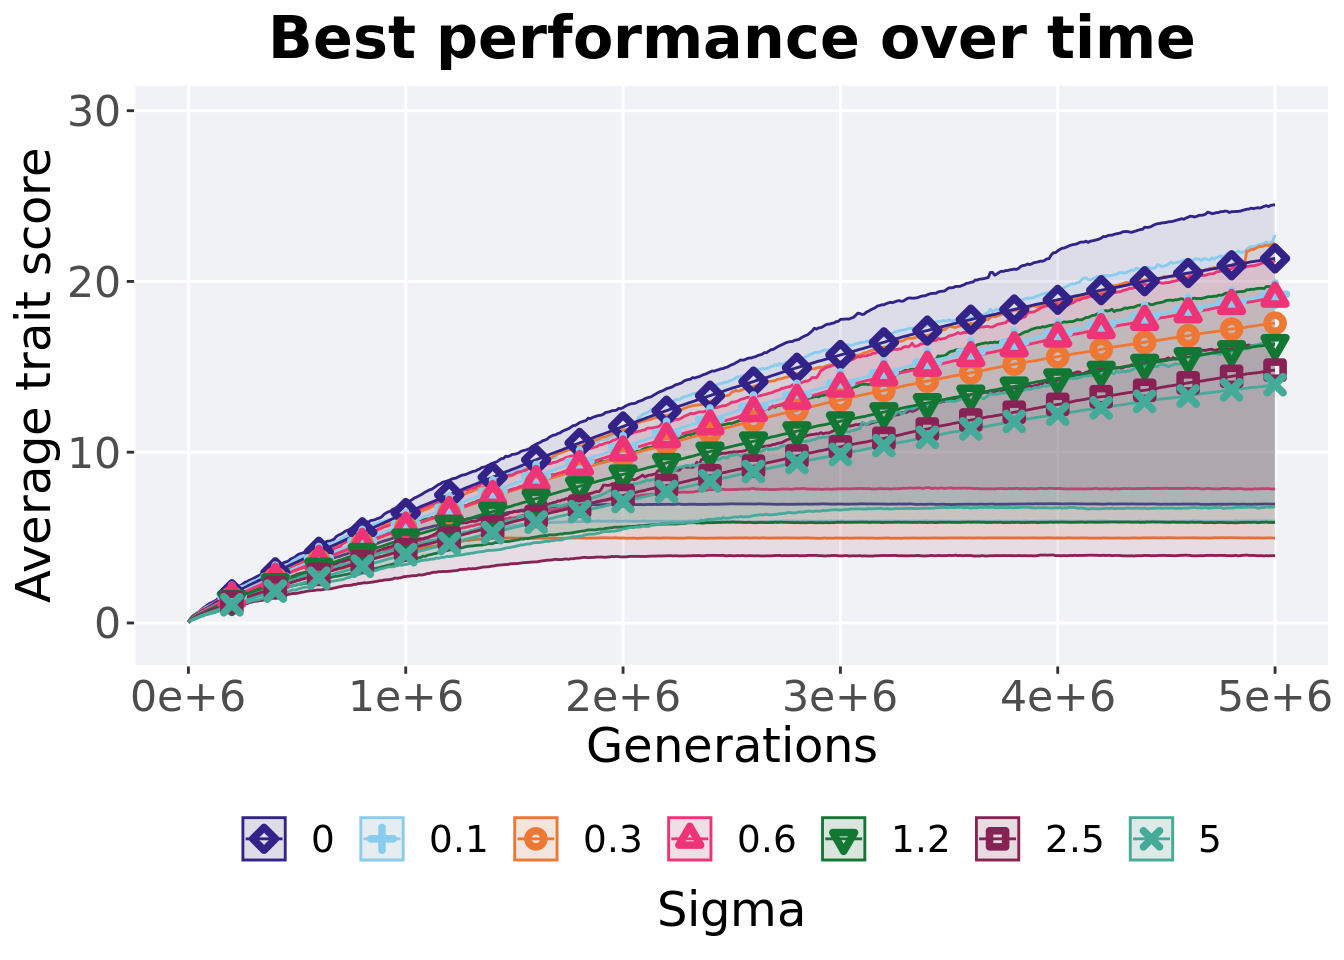
\includegraphics{demo_files/figure-latex/unnamed-chunk-101-1.pdf}

\hypertarget{end-of-50000-generations-8}{%
\subsubsection{End of 50,000 generations}\label{end-of-50000-generations-8}}

Activation gene coverage in the population at the end of 50,000 generations.

\begin{Shaded}
\begin{Highlighting}[]
\NormalTok{end =}\StringTok{ }\KeywordTok{filter}\NormalTok{(tru_end, diagnostic }\OperatorTok{==}\StringTok{ 'multipath_exploration'}\NormalTok{)}
\NormalTok{plot =}\StringTok{ }\KeywordTok{ggplot}\NormalTok{(end, }\KeywordTok{aes}\NormalTok{(}\DataTypeTok{x =}\NormalTok{ T, }\DataTypeTok{y =}\NormalTok{ uni_str_pos, }\DataTypeTok{color =}\NormalTok{ T, }\DataTypeTok{fill =}\NormalTok{ T, }\DataTypeTok{shape =}\NormalTok{ T)) }\OperatorTok{+}
\StringTok{  }\KeywordTok{geom_flat_violin}\NormalTok{(}\DataTypeTok{position =} \KeywordTok{position_nudge}\NormalTok{(}\DataTypeTok{x =} \FloatTok{.2}\NormalTok{, }\DataTypeTok{y =} \DecValTok{0}\NormalTok{), }\DataTypeTok{scale =} \StringTok{'width'}\NormalTok{, }\DataTypeTok{alpha =} \FloatTok{0.2}\NormalTok{) }\OperatorTok{+}
\StringTok{  }\KeywordTok{geom_point}\NormalTok{(}\DataTypeTok{position =} \KeywordTok{position_jitter}\NormalTok{(}\DataTypeTok{width =} \FloatTok{.1}\NormalTok{), }\DataTypeTok{size =} \FloatTok{1.5}\NormalTok{, }\DataTypeTok{alpha =} \FloatTok{1.0}\NormalTok{) }\OperatorTok{+}
\StringTok{  }\KeywordTok{geom_boxplot}\NormalTok{(}\DataTypeTok{color =} \StringTok{'black'}\NormalTok{, }\DataTypeTok{width =} \FloatTok{.2}\NormalTok{, }\DataTypeTok{outlier.shape =} \OtherTok{NA}\NormalTok{, }\DataTypeTok{alpha =} \FloatTok{0.0}\NormalTok{) }\OperatorTok{+}
\StringTok{  }\KeywordTok{scale_y_continuous}\NormalTok{(}
    \DataTypeTok{name=}\StringTok{"Coverage"}\NormalTok{,}
    \DataTypeTok{limits=}\KeywordTok{c}\NormalTok{(}\OperatorTok{-}\DecValTok{1}\NormalTok{, }\DecValTok{10}\NormalTok{),}
    \DataTypeTok{breaks=}\KeywordTok{seq}\NormalTok{(}\DecValTok{0}\NormalTok{,}\DecValTok{10}\NormalTok{, }\DecValTok{2}\NormalTok{),}
    \DataTypeTok{labels=}\KeywordTok{c}\NormalTok{(}\StringTok{"0"}\NormalTok{, }\StringTok{"2"}\NormalTok{, }\StringTok{"4"}\NormalTok{, }\StringTok{"6"}\NormalTok{, }\StringTok{"8"}\NormalTok{, }\StringTok{"10"}\NormalTok{)}
\NormalTok{  ) }\OperatorTok{+}
\StringTok{  }\KeywordTok{scale_x_discrete}\NormalTok{(}
    \DataTypeTok{name=}\StringTok{"T"}
\NormalTok{  )}\OperatorTok{+}
\StringTok{  }\KeywordTok{scale_shape_manual}\NormalTok{(}\DataTypeTok{values=}\NormalTok{SHAPE)}\OperatorTok{+}
\StringTok{  }\KeywordTok{scale_colour_manual}\NormalTok{(}\DataTypeTok{values =}\NormalTok{ cb_palette) }\OperatorTok{+}
\StringTok{  }\KeywordTok{scale_fill_manual}\NormalTok{(}\DataTypeTok{values =}\NormalTok{ cb_palette) }\OperatorTok{+}
\StringTok{  }\NormalTok{p_theme}

\KeywordTok{plot_grid}\NormalTok{(}
\NormalTok{  plot }\OperatorTok{+}
\StringTok{    }\KeywordTok{ggtitle}\NormalTok{(}\StringTok{"Final activation gene coverage"}\NormalTok{) }\OperatorTok{+}
\StringTok{    }\KeywordTok{theme}\NormalTok{(}\DataTypeTok{legend.position=}\StringTok{"none"}\NormalTok{),}
\NormalTok{  legend,}
  \DataTypeTok{nrow=}\DecValTok{2}\NormalTok{,}
  \DataTypeTok{rel_heights =} \KeywordTok{c}\NormalTok{(}\DecValTok{2}\NormalTok{,.}\DecValTok{3}\NormalTok{),}
  \DataTypeTok{label_size =}\NormalTok{ TSIZE}
\NormalTok{)}
\end{Highlighting}
\end{Shaded}

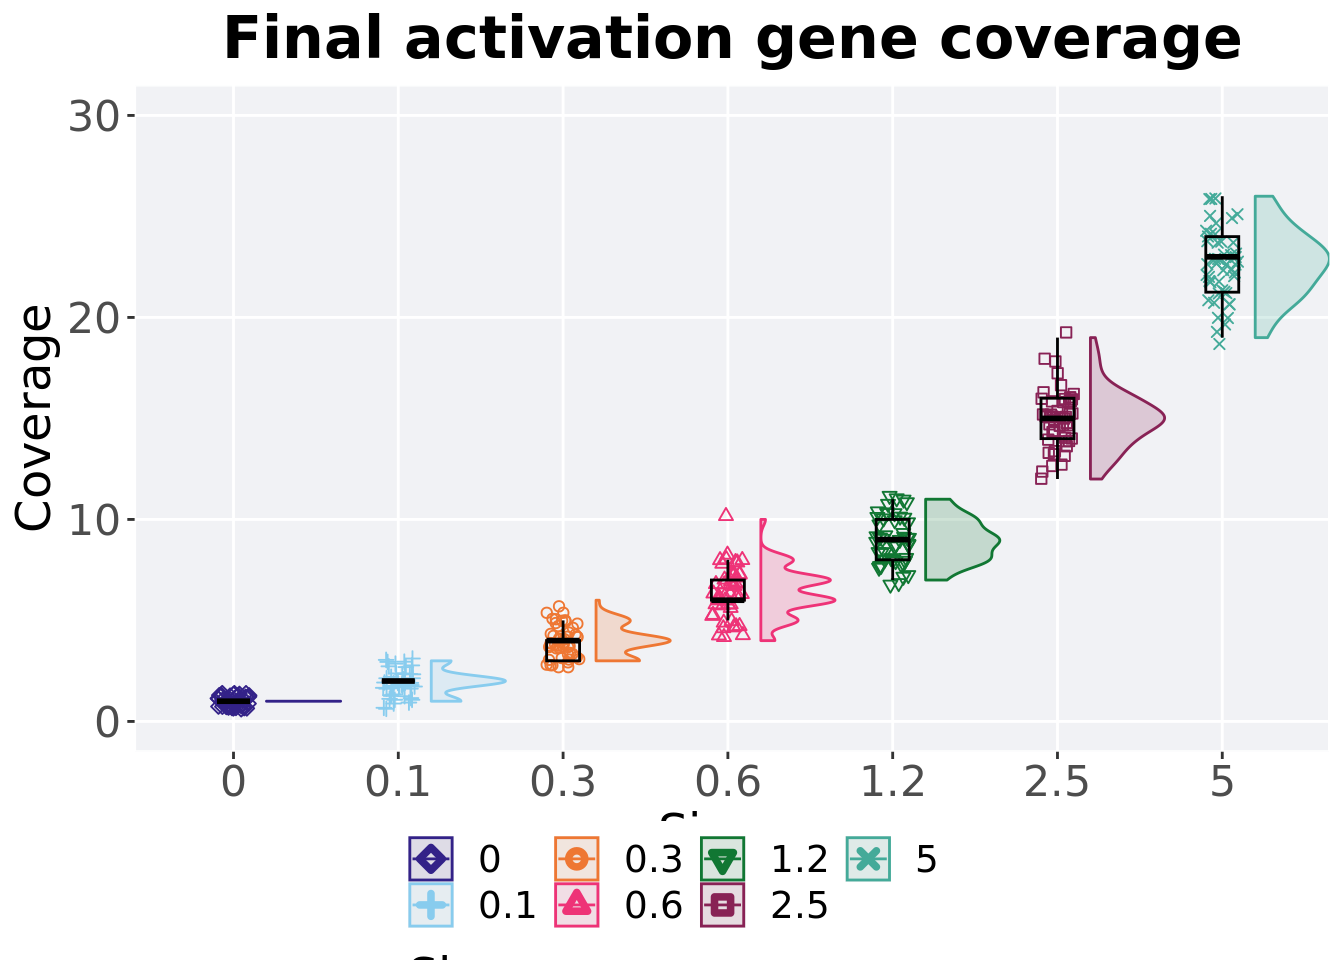
\includegraphics{demo_files/figure-latex/unnamed-chunk-102-1.pdf}

\hypertarget{stats-19}{%
\paragraph{Stats}\label{stats-19}}

Summary statistics for the activation gene coverage in the population at the end of 50,000 generations.

\begin{Shaded}
\begin{Highlighting}[]
\KeywordTok{group_by}\NormalTok{(end, T) }\OperatorTok
\StringTok{  }\NormalTok{dplyr}\OperatorTok{::}\KeywordTok{summarise}\NormalTok{(}
    \DataTypeTok{count =} \KeywordTok{n}\NormalTok{(),}
    \DataTypeTok{na_cnt =} \KeywordTok{sum}\NormalTok{(}\KeywordTok{is.na}\NormalTok{(uni_str_pos)),}
    \DataTypeTok{min =} \KeywordTok{min}\NormalTok{(uni_str_pos, }\DataTypeTok{na.rm =} \OtherTok{TRUE}\NormalTok{),}
    \DataTypeTok{median =} \KeywordTok{median}\NormalTok{(uni_str_pos, }\DataTypeTok{na.rm =} \OtherTok{TRUE}\NormalTok{),}
    \DataTypeTok{mean =} \KeywordTok{mean}\NormalTok{(uni_str_pos, }\DataTypeTok{na.rm =} \OtherTok{TRUE}\NormalTok{),}
    \DataTypeTok{max =} \KeywordTok{max}\NormalTok{(uni_str_pos, }\DataTypeTok{na.rm =} \OtherTok{TRUE}\NormalTok{),}
    \DataTypeTok{IQR =} \KeywordTok{IQR}\NormalTok{(uni_str_pos, }\DataTypeTok{na.rm =} \OtherTok{TRUE}\NormalTok{)}
\NormalTok{  )}
\end{Highlighting}
\end{Shaded}

\begin{verbatim}
## # A tibble: 9 x 8
##   T     count na_cnt   min median  mean   max   IQR
##   <fct> <int>  <int> <int>  <dbl> <dbl> <int> <dbl>
## 1 1        50      0     2      2  2.02     3     0
## 2 2        50      0     1      2  2        3     0
## 3 4        50      0     2      2  2        2     0
## 4 8        50      0     1      2  2        3     0
## 5 16       50      0     2      2  2        2     0
## 6 32       50      0     1      2  1.98     3     0
## 7 64       50      0     1      2  1.98     3     0
## 8 128      50      0     1      2  2.04     3     0
## 9 256      50      0     1      2  2.22     4     0
\end{verbatim}

Kruskal--Wallis test provides evidence of statistical differences among activation gene coverage in the population at the end of 50,000 generations.

\begin{Shaded}
\begin{Highlighting}[]
\KeywordTok{kruskal.test}\NormalTok{(uni_str_pos }\OperatorTok{~}\StringTok{ }\NormalTok{T, }\DataTypeTok{data =}\NormalTok{ end)}
\end{Highlighting}
\end{Shaded}

\begin{verbatim}
## 
##  Kruskal-Wallis rank sum test
## 
## data:  uni_str_pos by T
## Kruskal-Wallis chi-squared = 19.931, df = 8, p-value = 0.0106
\end{verbatim}

Results for post-hoc Wilcoxon rank-sum test with a Bonferroni correction on the activation gene coverage in the population at the end of 50,000 generations.

\begin{Shaded}
\begin{Highlighting}[]
\KeywordTok{pairwise.wilcox.test}\NormalTok{(}\DataTypeTok{x =}\NormalTok{ end}\OperatorTok{$}\NormalTok{uni_str_pos, }\DataTypeTok{g =}\NormalTok{ end}\OperatorTok{$}\NormalTok{T , }\DataTypeTok{p.adjust.method =} \StringTok{"bonferroni"}\NormalTok{,}
                     \DataTypeTok{paired =} \OtherTok{FALSE}\NormalTok{, }\DataTypeTok{conf.int =} \OtherTok{FALSE}\NormalTok{, }\DataTypeTok{alternative =} \StringTok{'t'}\NormalTok{)}
\end{Highlighting}
\end{Shaded}

\begin{verbatim}
## 
##  Pairwise comparisons using Wilcoxon rank sum test with continuity correction 
## 
## data:  end$uni_str_pos and end$T 
## 
##     1    2    4    8    16   32   64   128 
## 2   1.00 -    -    -    -    -    -    -   
## 4   1.00 1.00 -    -    -    -    -    -   
## 8   1.00 1.00 1.00 -    -    -    -    -   
## 16  1.00 1.00 -    1.00 -    -    -    -   
## 32  1.00 1.00 1.00 1.00 1.00 -    -    -   
## 64  1.00 1.00 1.00 1.00 1.00 1.00 -    -   
## 128 1.00 1.00 1.00 1.00 1.00 1.00 1.00 -   
## 256 1.00 0.85 0.52 0.85 0.52 0.56 0.83 1.00
## 
## P value adjustment method: bonferroni
\end{verbatim}

\hypertarget{tournament-selection}{%
\chapter{Tournament selection}\label{tournament-selection}}

We present the results from our parameter sweeep on tournament selection.
50 replicates are conducted for each tournament size \texttt{T} parameter value explored.

\begin{Shaded}
\begin{Highlighting}[]
\KeywordTok{library}\NormalTok{(ggplot2)}
\KeywordTok{library}\NormalTok{(cowplot)}
\KeywordTok{library}\NormalTok{(dplyr)}
\KeywordTok{library}\NormalTok{(PupillometryR)}
\end{Highlighting}
\end{Shaded}

These analyses were conducted in the following computing environment:

\begin{Shaded}
\begin{Highlighting}[]
\KeywordTok{print}\NormalTok{(version)}
\end{Highlighting}
\end{Shaded}

\begin{verbatim}
##                _                           
## platform       x86_64-pc-linux-gnu         
## arch           x86_64                      
## os             linux-gnu                   
## system         x86_64, linux-gnu           
## status                                     
## major          4                           
## minor          2.1                         
## year           2022                        
## month          06                          
## day            23                          
## svn rev        82513                       
## language       R                           
## version.string R version 4.2.1 (2022-06-23)
## nickname       Funny-Looking Kid
\end{verbatim}

\hypertarget{exploitation-rate-results-2}{%
\section{Exploitation rate results}\label{exploitation-rate-results-2}}

Here we present the results for \textbf{best performances} found by each tournament selection value replicate on the exploitation rate diagnostic.

\hypertarget{performance-over-time-5}{%
\subsection{Performance over time}\label{performance-over-time-5}}

Performance over time.

\begin{Shaded}
\begin{Highlighting}[]
\NormalTok{problem <-}\StringTok{ }\KeywordTok{filter}\NormalTok{(tor_ot, diagnostic }\OperatorTok{==}\StringTok{ 'exploitation_rate'}\NormalTok{)}
\NormalTok{lines =}\StringTok{ }\NormalTok{problem }\OperatorTok
\StringTok{        }\KeywordTok{group_by}\NormalTok{(T, gen) }\OperatorTok
\StringTok{          }\NormalTok{dplyr}\OperatorTok{::}\KeywordTok{summarise}\NormalTok{(}
            \DataTypeTok{min =} \KeywordTok{min}\NormalTok{(pop_fit_max),}
            \DataTypeTok{mean =} \KeywordTok{mean}\NormalTok{(pop_fit_max),}
            \DataTypeTok{max =} \KeywordTok{max}\NormalTok{(pop_fit_max)}
\NormalTok{          )}
\end{Highlighting}
\end{Shaded}

\begin{verbatim}
## `summarise()` has grouped output by 'T'. You can override using the `.groups`
## argument.
\end{verbatim}

\begin{Shaded}
\begin{Highlighting}[]
\NormalTok{points =}\StringTok{ }\KeywordTok{filter}\NormalTok{(lines, gen }\OperatorTok\StringTok{ }\DecValTok{2000} \OperatorTok{==}\StringTok{ }\DecValTok{0} \OperatorTok{&}\StringTok{ }\NormalTok{gen }\OperatorTok{!=}\StringTok{ }\DecValTok{0}\NormalTok{)}

\NormalTok{ot =}\StringTok{ }\KeywordTok{ggplot}\NormalTok{(lines, }\KeywordTok{aes}\NormalTok{(}\DataTypeTok{x=}\NormalTok{gen, }\DataTypeTok{y=}\NormalTok{mean }\OperatorTok{/}\StringTok{ }\NormalTok{TRAITS, }\DataTypeTok{group =}\NormalTok{ T, }\DataTypeTok{fill =}\NormalTok{ T, }\DataTypeTok{color =}\NormalTok{ T, }\DataTypeTok{shape =}\NormalTok{ T)) }\OperatorTok{+}
\StringTok{  }\KeywordTok{geom_ribbon}\NormalTok{(}\KeywordTok{aes}\NormalTok{(}\DataTypeTok{ymin =}\NormalTok{ min }\OperatorTok{/}\StringTok{ }\NormalTok{TRAITS, }\DataTypeTok{ymax =}\NormalTok{ max }\OperatorTok{/}\StringTok{ }\NormalTok{TRAITS), }\DataTypeTok{alpha =} \FloatTok{0.1}\NormalTok{) }\OperatorTok{+}
\StringTok{  }\KeywordTok{geom_line}\NormalTok{(}\DataTypeTok{size =} \FloatTok{0.5}\NormalTok{) }\OperatorTok{+}
\StringTok{  }\KeywordTok{geom_point}\NormalTok{(}\DataTypeTok{data =}\NormalTok{ points, }\DataTypeTok{size =} \FloatTok{1.5}\NormalTok{, }\DataTypeTok{stroke =} \FloatTok{2.0}\NormalTok{, }\DataTypeTok{alpha =} \FloatTok{1.0}\NormalTok{) }\OperatorTok{+}
\StringTok{  }\KeywordTok{scale_y_continuous}\NormalTok{(}
    \DataTypeTok{name=}\StringTok{"Average trait score"}\NormalTok{,}
    \DataTypeTok{limits=}\KeywordTok{c}\NormalTok{(}\OperatorTok{-}\DecValTok{1}\NormalTok{, }\DecValTok{101}\NormalTok{),}
    \DataTypeTok{breaks=}\KeywordTok{seq}\NormalTok{(}\DecValTok{0}\NormalTok{,}\DecValTok{100}\NormalTok{, }\DecValTok{20}\NormalTok{),}
    \DataTypeTok{labels=}\KeywordTok{c}\NormalTok{(}\StringTok{"0"}\NormalTok{, }\StringTok{"20"}\NormalTok{, }\StringTok{"40"}\NormalTok{, }\StringTok{"60"}\NormalTok{, }\StringTok{"80"}\NormalTok{, }\StringTok{"100"}\NormalTok{)}
\NormalTok{  ) }\OperatorTok{+}
\StringTok{  }\KeywordTok{scale_x_continuous}\NormalTok{(}
    \DataTypeTok{name=}\StringTok{"Generations"}\NormalTok{,}
    \DataTypeTok{limits=}\KeywordTok{c}\NormalTok{(}\DecValTok{0}\NormalTok{, }\DecValTok{50000}\NormalTok{),}
    \DataTypeTok{breaks=}\KeywordTok{c}\NormalTok{(}\DecValTok{0}\NormalTok{, }\DecValTok{10000}\NormalTok{, }\DecValTok{20000}\NormalTok{, }\DecValTok{30000}\NormalTok{, }\DecValTok{40000}\NormalTok{, }\DecValTok{50000}\NormalTok{),}
    \DataTypeTok{labels=}\KeywordTok{c}\NormalTok{(}\StringTok{"0e+6"}\NormalTok{, }\StringTok{"1e+6"}\NormalTok{, }\StringTok{"2e+6"}\NormalTok{, }\StringTok{"3e+6"}\NormalTok{, }\StringTok{"4e+6"}\NormalTok{, }\StringTok{"5e+6"}\NormalTok{)}

\NormalTok{  ) }\OperatorTok{+}
\StringTok{  }\KeywordTok{scale_shape_manual}\NormalTok{(}\DataTypeTok{values=}\NormalTok{SHAPE)}\OperatorTok{+}
\StringTok{  }\KeywordTok{scale_colour_manual}\NormalTok{(}\DataTypeTok{values =}\NormalTok{ cb_palette) }\OperatorTok{+}
\StringTok{  }\KeywordTok{scale_fill_manual}\NormalTok{(}\DataTypeTok{values =}\NormalTok{ cb_palette) }\OperatorTok{+}
\StringTok{  }\KeywordTok{ggtitle}\NormalTok{(}\StringTok{"Best performance over time"}\NormalTok{) }\OperatorTok{+}
\StringTok{  }\NormalTok{p_theme}\OperatorTok{+}
\StringTok{    }\KeywordTok{guides}\NormalTok{(}
    \DataTypeTok{shape=}\KeywordTok{guide_legend}\NormalTok{(}\DataTypeTok{nrow=}\DecValTok{1}\NormalTok{, }\DataTypeTok{title.position =} \StringTok{"bottom"}\NormalTok{),}
    \DataTypeTok{color=}\KeywordTok{guide_legend}\NormalTok{(}\DataTypeTok{nrow=}\DecValTok{1}\NormalTok{, }\DataTypeTok{title.position =} \StringTok{"bottom"}\NormalTok{),}
    \DataTypeTok{fill=}\KeywordTok{guide_legend}\NormalTok{(}\DataTypeTok{nrow=}\DecValTok{1}\NormalTok{, }\DataTypeTok{title.position =} \StringTok{"bottom"}\NormalTok{)}
\NormalTok{  ) }\OperatorTok{+}
\StringTok{  }\KeywordTok{theme}\NormalTok{(}
    \DataTypeTok{legend.position =} \StringTok{"bottom"}\NormalTok{,}
    \DataTypeTok{legend.box=}\StringTok{"verticle"}\NormalTok{,}
    \DataTypeTok{legend.justification=}\StringTok{"center"}\NormalTok{,}
    \DataTypeTok{legend.title.align=}\FloatTok{0.5}
\NormalTok{  )}

\NormalTok{ot}
\end{Highlighting}
\end{Shaded}

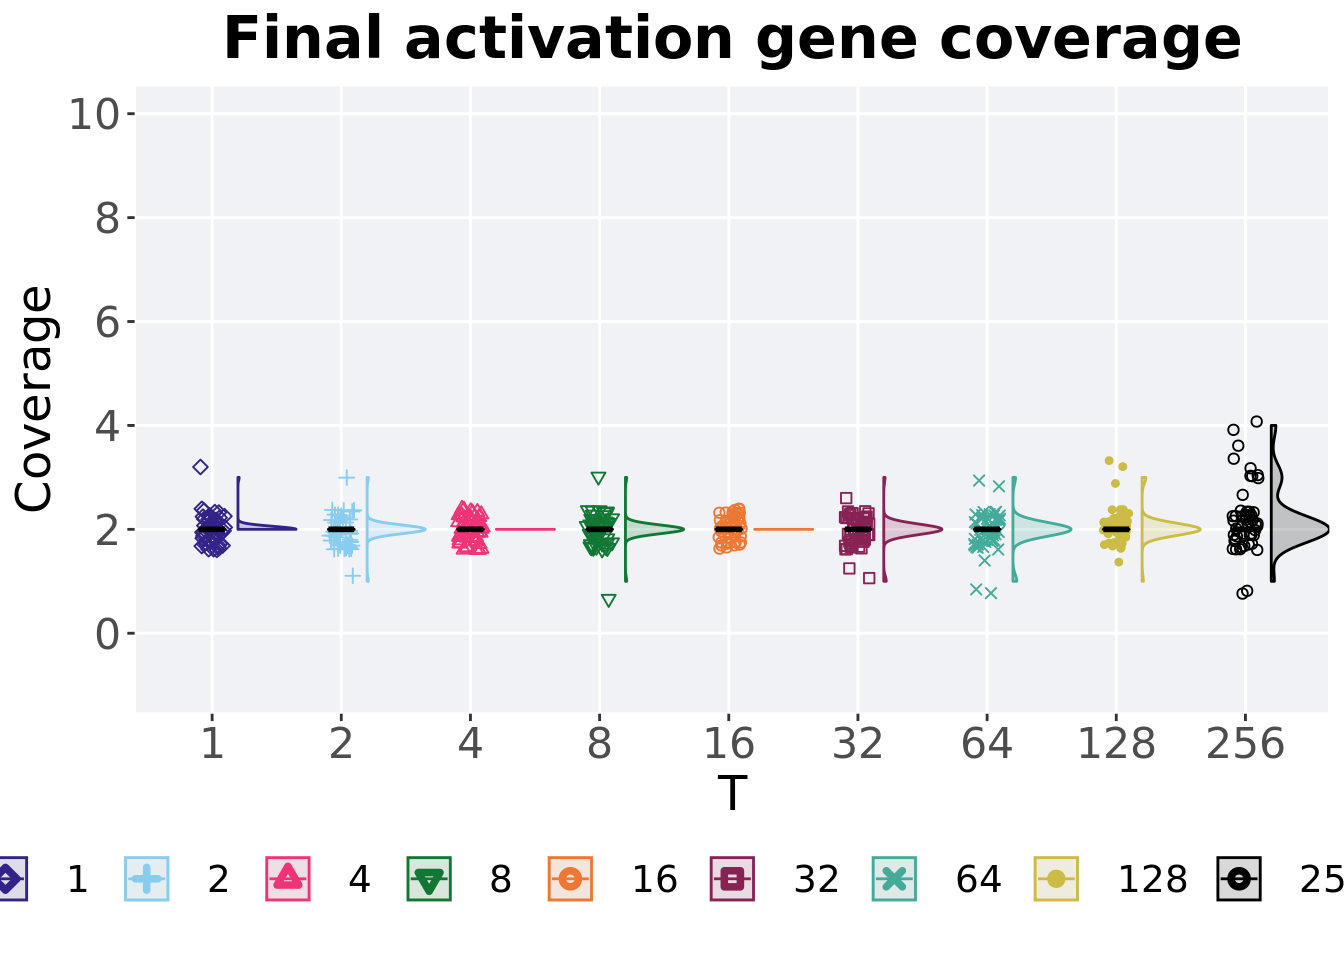
\includegraphics{demo_files/figure-latex/unnamed-chunk-108-1.pdf}

\hypertarget{generation-satisfactory-solution-found-4}{%
\subsection{Generation satisfactory solution found}\label{generation-satisfactory-solution-found-4}}

The first generation a satisfactory solution is found throughout the 50,000 generations.

\begin{Shaded}
\begin{Highlighting}[]
\NormalTok{ssf =}\StringTok{ }\KeywordTok{filter}\NormalTok{(tor_ssf, diagnostic }\OperatorTok{==}\StringTok{ 'exploitation_rate'}\NormalTok{)}

\NormalTok{plot <-}\StringTok{ }\KeywordTok{ggplot}\NormalTok{(ssf, }\KeywordTok{aes}\NormalTok{(}\DataTypeTok{x =}\NormalTok{ T, }\DataTypeTok{y =}\NormalTok{ generation, }\DataTypeTok{color =}\NormalTok{ T, }\DataTypeTok{fill =}\NormalTok{ T, }\DataTypeTok{shape =}\NormalTok{ T)) }\OperatorTok{+}
\StringTok{  }\KeywordTok{geom_flat_violin}\NormalTok{(}\DataTypeTok{position =} \KeywordTok{position_nudge}\NormalTok{(}\DataTypeTok{x =} \FloatTok{.2}\NormalTok{, }\DataTypeTok{y =} \DecValTok{0}\NormalTok{), }\DataTypeTok{scale =} \StringTok{'width'}\NormalTok{, }\DataTypeTok{alpha =} \FloatTok{0.2}\NormalTok{) }\OperatorTok{+}
\StringTok{  }\KeywordTok{geom_point}\NormalTok{(}\DataTypeTok{position =} \KeywordTok{position_jitter}\NormalTok{(}\DataTypeTok{width =} \FloatTok{.1}\NormalTok{), }\DataTypeTok{size =} \FloatTok{1.5}\NormalTok{, }\DataTypeTok{alpha =} \FloatTok{1.0}\NormalTok{) }\OperatorTok{+}
\StringTok{  }\KeywordTok{geom_boxplot}\NormalTok{(}\DataTypeTok{color =} \StringTok{'black'}\NormalTok{, }\DataTypeTok{width =} \FloatTok{.2}\NormalTok{, }\DataTypeTok{outlier.shape =} \OtherTok{NA}\NormalTok{, }\DataTypeTok{alpha =} \FloatTok{0.0}\NormalTok{) }\OperatorTok{+}
\StringTok{  }\KeywordTok{scale_shape_manual}\NormalTok{(}\DataTypeTok{values=}\NormalTok{SHAPE)}\OperatorTok{+}
\StringTok{  }\KeywordTok{scale_y_continuous}\NormalTok{(}
    \DataTypeTok{name=}\StringTok{"Generation"}\NormalTok{,}
    \DataTypeTok{limits=}\KeywordTok{c}\NormalTok{(}\DecValTok{0}\NormalTok{, }\DecValTok{12000}\NormalTok{),}
    \DataTypeTok{breaks=}\KeywordTok{c}\NormalTok{(}\DecValTok{0}\NormalTok{, }\DecValTok{2000}\NormalTok{, }\DecValTok{4000}\NormalTok{, }\DecValTok{6000}\NormalTok{, }\DecValTok{8000}\NormalTok{, }\DecValTok{10000}\NormalTok{, }\DecValTok{12000}\NormalTok{),}
    \DataTypeTok{labels=}\KeywordTok{c}\NormalTok{(}\StringTok{"0e+6"}\NormalTok{, }\StringTok{"2e+6"}\NormalTok{, }\StringTok{"4e+6"}\NormalTok{, }\StringTok{"6e+6"}\NormalTok{, }\StringTok{"8e+6"}\NormalTok{, }\StringTok{"10e+6"}\NormalTok{, }\StringTok{"12e+6"}\NormalTok{)}
\NormalTok{  ) }\OperatorTok{+}
\StringTok{  }\KeywordTok{scale_x_discrete}\NormalTok{(}
    \DataTypeTok{name=}\StringTok{"T"}
\NormalTok{  ) }\OperatorTok{+}
\StringTok{  }\KeywordTok{scale_colour_manual}\NormalTok{(}\DataTypeTok{values =}\NormalTok{ cb_palette) }\OperatorTok{+}
\StringTok{  }\KeywordTok{scale_fill_manual}\NormalTok{(}\DataTypeTok{values =}\NormalTok{ cb_palette) }\OperatorTok{+}
\StringTok{  }\NormalTok{p_theme}

\KeywordTok{plot_grid}\NormalTok{(}
\NormalTok{  plot }\OperatorTok{+}
\StringTok{    }\KeywordTok{ggtitle}\NormalTok{(}\StringTok{"Generation satisfactory solution found"}\NormalTok{) }\OperatorTok{+}
\StringTok{    }\KeywordTok{theme}\NormalTok{(}\DataTypeTok{legend.position=}\StringTok{"none"}\NormalTok{),}
\NormalTok{  legend,}
  \DataTypeTok{nrow=}\DecValTok{2}\NormalTok{,}
  \DataTypeTok{rel_heights =} \KeywordTok{c}\NormalTok{(}\DecValTok{2}\NormalTok{,.}\DecValTok{2}\NormalTok{),}
  \DataTypeTok{label_size =}\NormalTok{ TSIZE}
\NormalTok{)}
\end{Highlighting}
\end{Shaded}

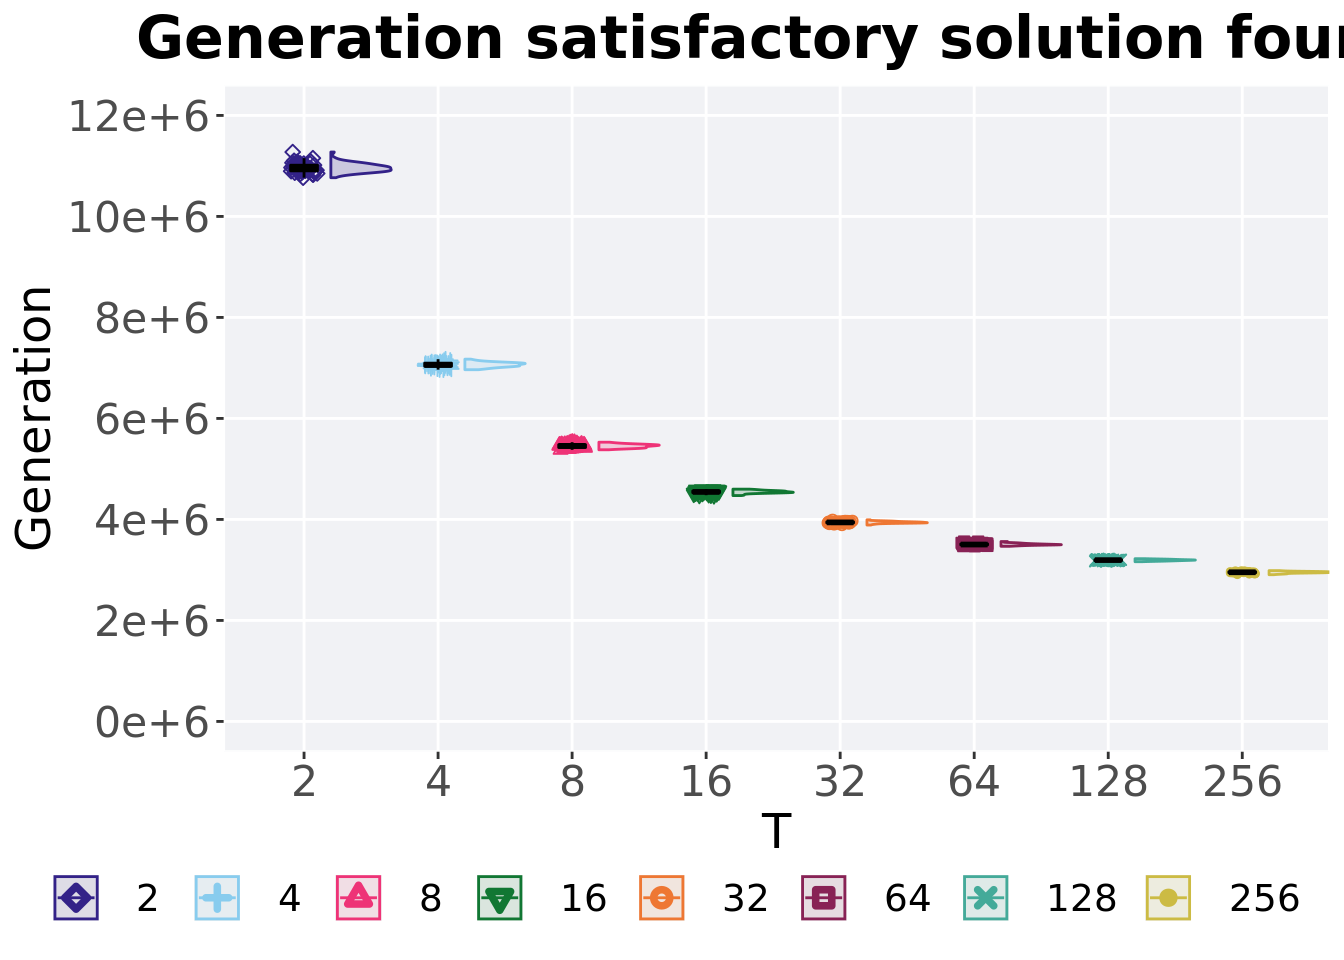
\includegraphics{demo_files/figure-latex/unnamed-chunk-110-1.pdf}

\hypertarget{stats-20}{%
\subsubsection{Stats}\label{stats-20}}

Summary statistics for the best performance found throughout 50,000 generations.

\begin{Shaded}
\begin{Highlighting}[]
\KeywordTok{group_by}\NormalTok{(ssf, T) }\OperatorTok
\StringTok{  }\NormalTok{dplyr}\OperatorTok{::}\KeywordTok{summarise}\NormalTok{(}
    \DataTypeTok{count =} \KeywordTok{n}\NormalTok{(),}
    \DataTypeTok{na_cnt =} \KeywordTok{sum}\NormalTok{(}\KeywordTok{is.na}\NormalTok{(generation)),}
    \DataTypeTok{min =} \KeywordTok{min}\NormalTok{(generation, }\DataTypeTok{na.rm =} \OtherTok{TRUE}\NormalTok{),}
    \DataTypeTok{median =} \KeywordTok{median}\NormalTok{(generation, }\DataTypeTok{na.rm =} \OtherTok{TRUE}\NormalTok{),}
    \DataTypeTok{mean =} \KeywordTok{mean}\NormalTok{(generation, }\DataTypeTok{na.rm =} \OtherTok{TRUE}\NormalTok{),}
    \DataTypeTok{max =} \KeywordTok{max}\NormalTok{(generation, }\DataTypeTok{na.rm =} \OtherTok{TRUE}\NormalTok{),}
    \DataTypeTok{IQR =} \KeywordTok{IQR}\NormalTok{(generation, }\DataTypeTok{na.rm =} \OtherTok{TRUE}\NormalTok{)}
\NormalTok{  )}
\end{Highlighting}
\end{Shaded}

\begin{verbatim}
## # A tibble: 8 x 8
##   T     count na_cnt   min median   mean   max   IQR
##   <fct> <int>  <int> <dbl>  <dbl>  <dbl> <dbl> <dbl>
## 1 2        50      0 10767 10964. 10963. 11275 112. 
## 2 4        50      0  6965  7059   7062.  7173  62.5
## 3 8        50      0  5379  5457   5453.  5529  56  
## 4 16       50      0  4472  4544   4545.  4599  34  
## 5 32       50      0  3889  3941   3941.  3992  21.5
## 6 64       50      0  3468  3502.  3506.  3562  20.8
## 7 128      50      0  3162  3194   3194.  3222  19.5
## 8 256      50      0  2905  2954.  2952.  2986  21.5
\end{verbatim}

Kruskal--Wallis test provides evidence of significant differences among the generation a satisfactory solution is first found.

\begin{Shaded}
\begin{Highlighting}[]
\KeywordTok{kruskal.test}\NormalTok{(generation }\OperatorTok{~}\StringTok{ }\NormalTok{T,}\DataTypeTok{data =}\NormalTok{ ssf)}
\end{Highlighting}
\end{Shaded}

\begin{verbatim}
## 
##  Kruskal-Wallis rank sum test
## 
## data:  generation by T
## Kruskal-Wallis chi-squared = 392.77, df = 7, p-value < 2.2e-16
\end{verbatim}

Results for post-hoc Wilcoxon rank-sum test with a Bonferroni correction on the generation a satisfactory solution is first found. .

\begin{Shaded}
\begin{Highlighting}[]
\KeywordTok{pairwise.wilcox.test}\NormalTok{(}\DataTypeTok{x =}\NormalTok{ ssf}\OperatorTok{$}\NormalTok{generation, }\DataTypeTok{g =}\NormalTok{ ssf}\OperatorTok{$}\NormalTok{T , }\DataTypeTok{p.adjust.method =} \StringTok{"bonferroni"}\NormalTok{,}
                     \DataTypeTok{paired =} \OtherTok{FALSE}\NormalTok{, }\DataTypeTok{conf.int =} \OtherTok{FALSE}\NormalTok{, }\DataTypeTok{alternative =} \StringTok{'l'}\NormalTok{)}
\end{Highlighting}
\end{Shaded}

\begin{verbatim}
## 
##  Pairwise comparisons using Wilcoxon rank sum test with continuity correction 
## 
## data:  ssf$generation and ssf$T 
## 
##     2      4      8      16     32     64     128   
## 4   <2e-16 -      -      -      -      -      -     
## 8   <2e-16 <2e-16 -      -      -      -      -     
## 16  <2e-16 <2e-16 <2e-16 -      -      -      -     
## 32  <2e-16 <2e-16 <2e-16 <2e-16 -      -      -     
## 64  <2e-16 <2e-16 <2e-16 <2e-16 <2e-16 -      -     
## 128 <2e-16 <2e-16 <2e-16 <2e-16 <2e-16 <2e-16 -     
## 256 <2e-16 <2e-16 <2e-16 <2e-16 <2e-16 <2e-16 <2e-16
## 
## P value adjustment method: bonferroni
\end{verbatim}

\hypertarget{ordered-exploitation-results-2}{%
\section{Ordered exploitation results}\label{ordered-exploitation-results-2}}

Here we present the results for \textbf{best performances} found by each genotypic fitness sharing sigma value replicate on the ordered exploitation diagnostic.
Best performance found refers to the largest average trait score found in a given population.
Note that performance values fall between 0 and 100.

\hypertarget{performance-over-time-6}{%
\subsection{Performance over time}\label{performance-over-time-6}}

Performance over time.

\begin{Shaded}
\begin{Highlighting}[]
\NormalTok{problem <-}\StringTok{ }\KeywordTok{filter}\NormalTok{(tor_ot, diagnostic }\OperatorTok{==}\StringTok{ 'ordered_exploitation'}\NormalTok{)}
\NormalTok{lines =}\StringTok{ }\NormalTok{problem }\OperatorTok
\StringTok{        }\KeywordTok{group_by}\NormalTok{(T, gen) }\OperatorTok
\StringTok{          }\NormalTok{dplyr}\OperatorTok{::}\KeywordTok{summarise}\NormalTok{(}
            \DataTypeTok{min =} \KeywordTok{min}\NormalTok{(pop_fit_max),}
            \DataTypeTok{mean =} \KeywordTok{mean}\NormalTok{(pop_fit_max),}
            \DataTypeTok{max =} \KeywordTok{max}\NormalTok{(pop_fit_max)}
\NormalTok{          )}
\end{Highlighting}
\end{Shaded}

\begin{verbatim}
## `summarise()` has grouped output by 'T'. You can override using the `.groups`
## argument.
\end{verbatim}

\begin{Shaded}
\begin{Highlighting}[]
\NormalTok{points =}\StringTok{ }\KeywordTok{filter}\NormalTok{(lines, gen }\OperatorTok\StringTok{ }\DecValTok{2000} \OperatorTok{==}\StringTok{ }\DecValTok{0} \OperatorTok{&}\StringTok{ }\NormalTok{gen }\OperatorTok{!=}\StringTok{ }\DecValTok{0}\NormalTok{)}

\NormalTok{ot =}\StringTok{ }\KeywordTok{ggplot}\NormalTok{(lines, }\KeywordTok{aes}\NormalTok{(}\DataTypeTok{x=}\NormalTok{gen, }\DataTypeTok{y=}\NormalTok{mean }\OperatorTok{/}\StringTok{ }\NormalTok{TRAITS, }\DataTypeTok{group =}\NormalTok{ T, }\DataTypeTok{fill =}\NormalTok{ T, }\DataTypeTok{color =}\NormalTok{ T, }\DataTypeTok{shape =}\NormalTok{ T)) }\OperatorTok{+}
\StringTok{  }\KeywordTok{geom_ribbon}\NormalTok{(}\KeywordTok{aes}\NormalTok{(}\DataTypeTok{ymin =}\NormalTok{ min }\OperatorTok{/}\StringTok{ }\NormalTok{TRAITS, }\DataTypeTok{ymax =}\NormalTok{ max }\OperatorTok{/}\StringTok{ }\NormalTok{TRAITS), }\DataTypeTok{alpha =} \FloatTok{0.1}\NormalTok{) }\OperatorTok{+}
\StringTok{  }\KeywordTok{geom_line}\NormalTok{(}\DataTypeTok{size =} \FloatTok{0.5}\NormalTok{) }\OperatorTok{+}
\StringTok{  }\KeywordTok{geom_point}\NormalTok{(}\DataTypeTok{data =}\NormalTok{ points, }\DataTypeTok{size =} \FloatTok{1.5}\NormalTok{, }\DataTypeTok{stroke =} \FloatTok{2.0}\NormalTok{, }\DataTypeTok{alpha =} \FloatTok{1.0}\NormalTok{) }\OperatorTok{+}
\StringTok{  }\KeywordTok{scale_y_continuous}\NormalTok{(}
    \DataTypeTok{name=}\StringTok{"Average trait score"}\NormalTok{,}
    \DataTypeTok{limits=}\KeywordTok{c}\NormalTok{(}\OperatorTok{-}\DecValTok{1}\NormalTok{, }\DecValTok{101}\NormalTok{),}
    \DataTypeTok{breaks=}\KeywordTok{seq}\NormalTok{(}\DecValTok{0}\NormalTok{,}\DecValTok{100}\NormalTok{, }\DecValTok{20}\NormalTok{),}
    \DataTypeTok{labels=}\KeywordTok{c}\NormalTok{(}\StringTok{"0"}\NormalTok{, }\StringTok{"20"}\NormalTok{, }\StringTok{"40"}\NormalTok{, }\StringTok{"60"}\NormalTok{, }\StringTok{"80"}\NormalTok{, }\StringTok{"100"}\NormalTok{)}
\NormalTok{  ) }\OperatorTok{+}
\StringTok{  }\KeywordTok{scale_x_continuous}\NormalTok{(}
    \DataTypeTok{name=}\StringTok{"Generations"}\NormalTok{,}
    \DataTypeTok{limits=}\KeywordTok{c}\NormalTok{(}\DecValTok{0}\NormalTok{, }\DecValTok{50000}\NormalTok{),}
    \DataTypeTok{breaks=}\KeywordTok{c}\NormalTok{(}\DecValTok{0}\NormalTok{, }\DecValTok{10000}\NormalTok{, }\DecValTok{20000}\NormalTok{, }\DecValTok{30000}\NormalTok{, }\DecValTok{40000}\NormalTok{, }\DecValTok{50000}\NormalTok{),}
    \DataTypeTok{labels=}\KeywordTok{c}\NormalTok{(}\StringTok{"0e+6"}\NormalTok{, }\StringTok{"1e+6"}\NormalTok{, }\StringTok{"2e+6"}\NormalTok{, }\StringTok{"3e+6"}\NormalTok{, }\StringTok{"4e+6"}\NormalTok{, }\StringTok{"5e+6"}\NormalTok{)}

\NormalTok{  ) }\OperatorTok{+}
\StringTok{  }\KeywordTok{scale_shape_manual}\NormalTok{(}\DataTypeTok{values=}\NormalTok{SHAPE)}\OperatorTok{+}
\StringTok{  }\KeywordTok{scale_colour_manual}\NormalTok{(}\DataTypeTok{values =}\NormalTok{ cb_palette) }\OperatorTok{+}
\StringTok{  }\KeywordTok{scale_fill_manual}\NormalTok{(}\DataTypeTok{values =}\NormalTok{ cb_palette) }\OperatorTok{+}
\StringTok{  }\KeywordTok{ggtitle}\NormalTok{(}\StringTok{"Best performance over time"}\NormalTok{) }\OperatorTok{+}
\StringTok{  }\NormalTok{p_theme}\OperatorTok{+}
\StringTok{    }\KeywordTok{guides}\NormalTok{(}
    \DataTypeTok{shape=}\KeywordTok{guide_legend}\NormalTok{(}\DataTypeTok{nrow=}\DecValTok{1}\NormalTok{, }\DataTypeTok{title.position =} \StringTok{"bottom"}\NormalTok{),}
    \DataTypeTok{color=}\KeywordTok{guide_legend}\NormalTok{(}\DataTypeTok{nrow=}\DecValTok{1}\NormalTok{, }\DataTypeTok{title.position =} \StringTok{"bottom"}\NormalTok{),}
    \DataTypeTok{fill=}\KeywordTok{guide_legend}\NormalTok{(}\DataTypeTok{nrow=}\DecValTok{1}\NormalTok{, }\DataTypeTok{title.position =} \StringTok{"bottom"}\NormalTok{)}
\NormalTok{  ) }\OperatorTok{+}
\StringTok{  }\KeywordTok{theme}\NormalTok{(}
    \DataTypeTok{legend.position =} \StringTok{"bottom"}\NormalTok{,}
    \DataTypeTok{legend.box=}\StringTok{"verticle"}\NormalTok{,}
    \DataTypeTok{legend.justification=}\StringTok{"center"}\NormalTok{,}
    \DataTypeTok{legend.title.align=}\FloatTok{0.5}
\NormalTok{  )}

\NormalTok{ot}
\end{Highlighting}
\end{Shaded}

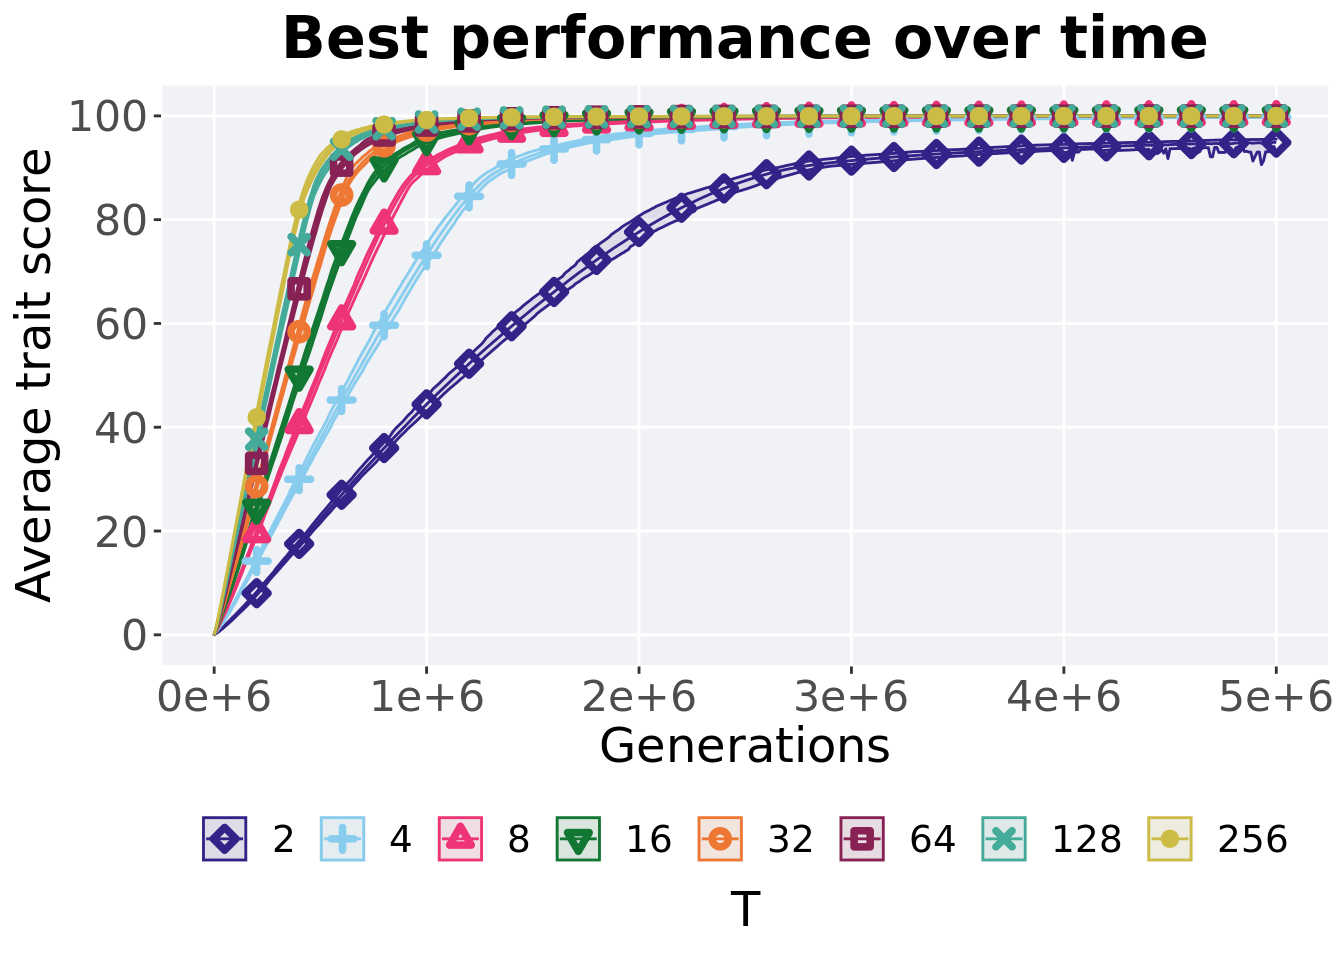
\includegraphics{demo_files/figure-latex/unnamed-chunk-114-1.pdf}

\hypertarget{generation-satisfactory-solution-found-5}{%
\subsection{Generation satisfactory solution found}\label{generation-satisfactory-solution-found-5}}

The first generation a satisfactory solution is found throughout the 50,000 generations.

\begin{Shaded}
\begin{Highlighting}[]
\NormalTok{ssf =}\StringTok{ }\KeywordTok{filter}\NormalTok{(tor_ssf, diagnostic }\OperatorTok{==}\StringTok{ 'ordered_exploitation'}\NormalTok{)}

\NormalTok{plot <-}\StringTok{ }\KeywordTok{ggplot}\NormalTok{(ssf, }\KeywordTok{aes}\NormalTok{(}\DataTypeTok{x =}\NormalTok{ T, }\DataTypeTok{y =}\NormalTok{ generation, }\DataTypeTok{color =}\NormalTok{ T, }\DataTypeTok{fill =}\NormalTok{ T, }\DataTypeTok{shape =}\NormalTok{ T)) }\OperatorTok{+}
\StringTok{  }\KeywordTok{geom_flat_violin}\NormalTok{(}\DataTypeTok{position =} \KeywordTok{position_nudge}\NormalTok{(}\DataTypeTok{x =} \FloatTok{.2}\NormalTok{, }\DataTypeTok{y =} \DecValTok{0}\NormalTok{), }\DataTypeTok{scale =} \StringTok{'width'}\NormalTok{, }\DataTypeTok{alpha =} \FloatTok{0.2}\NormalTok{) }\OperatorTok{+}
\StringTok{  }\KeywordTok{geom_point}\NormalTok{(}\DataTypeTok{position =} \KeywordTok{position_jitter}\NormalTok{(}\DataTypeTok{width =} \FloatTok{.1}\NormalTok{), }\DataTypeTok{size =} \FloatTok{1.5}\NormalTok{, }\DataTypeTok{alpha =} \FloatTok{1.0}\NormalTok{) }\OperatorTok{+}
\StringTok{  }\KeywordTok{geom_boxplot}\NormalTok{(}\DataTypeTok{color =} \StringTok{'black'}\NormalTok{, }\DataTypeTok{width =} \FloatTok{.2}\NormalTok{, }\DataTypeTok{outlier.shape =} \OtherTok{NA}\NormalTok{, }\DataTypeTok{alpha =} \FloatTok{0.0}\NormalTok{) }\OperatorTok{+}
\StringTok{  }\KeywordTok{scale_shape_manual}\NormalTok{(}\DataTypeTok{values=}\NormalTok{SHAPE)}\OperatorTok{+}
\StringTok{  }\KeywordTok{scale_y_continuous}\NormalTok{(}
    \DataTypeTok{name=}\StringTok{"Generation"}\NormalTok{,}
    \DataTypeTok{limits=}\KeywordTok{c}\NormalTok{(}\DecValTok{0}\NormalTok{, }\DecValTok{60000}\NormalTok{),}
    \DataTypeTok{breaks=}\KeywordTok{c}\NormalTok{(}\DecValTok{0}\NormalTok{, }\DecValTok{10000}\NormalTok{, }\DecValTok{20000}\NormalTok{, }\DecValTok{30000}\NormalTok{, }\DecValTok{40000}\NormalTok{, }\DecValTok{50000}\NormalTok{, }\DecValTok{60000}\NormalTok{),}
    \DataTypeTok{labels=}\KeywordTok{c}\NormalTok{(}\StringTok{"0e+6"}\NormalTok{, }\StringTok{"1e+6"}\NormalTok{, }\StringTok{"2e+6"}\NormalTok{, }\StringTok{"3e+6"}\NormalTok{, }\StringTok{"4e+6"}\NormalTok{, }\StringTok{"5e+6"}\NormalTok{, }\StringTok{"Fail"}\NormalTok{)}
\NormalTok{  ) }\OperatorTok{+}
\StringTok{  }\KeywordTok{scale_x_discrete}\NormalTok{(}
    \DataTypeTok{name=}\StringTok{"T"}
\NormalTok{  ) }\OperatorTok{+}
\StringTok{  }\KeywordTok{scale_colour_manual}\NormalTok{(}\DataTypeTok{values =}\NormalTok{ cb_palette) }\OperatorTok{+}
\StringTok{  }\KeywordTok{scale_fill_manual}\NormalTok{(}\DataTypeTok{values =}\NormalTok{ cb_palette) }\OperatorTok{+}
\StringTok{  }\NormalTok{p_theme}

\KeywordTok{plot_grid}\NormalTok{(}
\NormalTok{  plot }\OperatorTok{+}
\StringTok{    }\KeywordTok{ggtitle}\NormalTok{(}\StringTok{"Generation satisfactory solution found"}\NormalTok{) }\OperatorTok{+}
\StringTok{    }\KeywordTok{theme}\NormalTok{(}\DataTypeTok{legend.position=}\StringTok{"none"}\NormalTok{),}
\NormalTok{  legend,}
  \DataTypeTok{nrow=}\DecValTok{2}\NormalTok{,}
  \DataTypeTok{rel_heights =} \KeywordTok{c}\NormalTok{(}\DecValTok{2}\NormalTok{,.}\DecValTok{2}\NormalTok{),}
  \DataTypeTok{label_size =}\NormalTok{ TSIZE}
\NormalTok{)}
\end{Highlighting}
\end{Shaded}

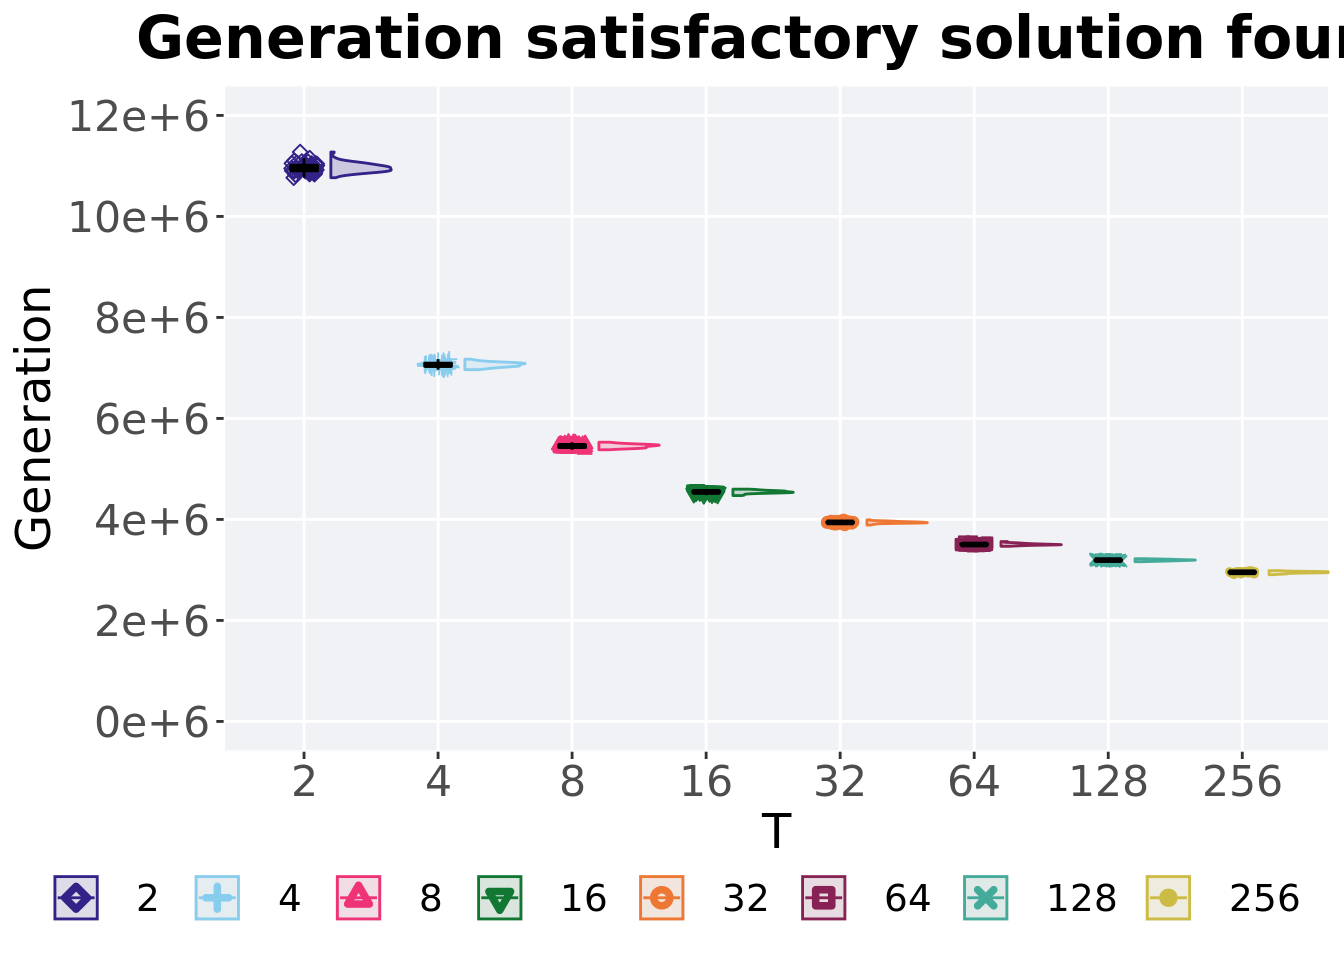
\includegraphics{demo_files/figure-latex/unnamed-chunk-116-1.pdf}

\hypertarget{stats-21}{%
\subsubsection{Stats}\label{stats-21}}

Summary statistics for the first generation a satisfactory solution is found throughout the 50,000 generations.

\begin{Shaded}
\begin{Highlighting}[]
\NormalTok{ssf =}\StringTok{ }\KeywordTok{filter}\NormalTok{(ssf, T }\OperatorTok{!=}\StringTok{ }\DecValTok{2}\NormalTok{)}

\KeywordTok{group_by}\NormalTok{(ssf, T) }\OperatorTok
\StringTok{  }\NormalTok{dplyr}\OperatorTok{::}\KeywordTok{summarise}\NormalTok{(}
    \DataTypeTok{count =} \KeywordTok{n}\NormalTok{(),}
    \DataTypeTok{na_cnt =} \KeywordTok{sum}\NormalTok{(}\KeywordTok{is.na}\NormalTok{(generation)),}
    \DataTypeTok{min =} \KeywordTok{min}\NormalTok{(generation, }\DataTypeTok{na.rm =} \OtherTok{TRUE}\NormalTok{),}
    \DataTypeTok{median =} \KeywordTok{median}\NormalTok{(generation, }\DataTypeTok{na.rm =} \OtherTok{TRUE}\NormalTok{),}
    \DataTypeTok{mean =} \KeywordTok{mean}\NormalTok{(generation, }\DataTypeTok{na.rm =} \OtherTok{TRUE}\NormalTok{),}
    \DataTypeTok{max =} \KeywordTok{max}\NormalTok{(generation, }\DataTypeTok{na.rm =} \OtherTok{TRUE}\NormalTok{),}
    \DataTypeTok{IQR =} \KeywordTok{IQR}\NormalTok{(generation, }\DataTypeTok{na.rm =} \OtherTok{TRUE}\NormalTok{)}
\NormalTok{  )}
\end{Highlighting}
\end{Shaded}

\begin{verbatim}
## # A tibble: 7 x 8
##   T     count na_cnt   min median   mean   max   IQR
##   <fct> <int>  <int> <dbl>  <dbl>  <dbl> <dbl> <dbl>
## 1 4        50      0 39186 41352. 41339. 43712 1474.
## 2 8        50      0 25283 26926. 26922. 28222  496.
## 3 16       50      0 20113 21130. 21135. 22015  642.
## 4 32       50      0 16732 17819  17821. 18957  499.
## 5 64       50      0 15028 15683  15722. 16562  608.
## 6 128      50      0 13171 14148. 14142. 14954  524 
## 7 256      50      0 11964 12546. 12548. 13104  402.
\end{verbatim}

Kruskal--Wallis test provides evidence of significant differences among the first generation a satisfactory solution is found throughout the 50,000 generations.

\begin{Shaded}
\begin{Highlighting}[]
\KeywordTok{kruskal.test}\NormalTok{(generation }\OperatorTok{~}\StringTok{ }\NormalTok{T, }\DataTypeTok{data =}\NormalTok{ ssf)}
\end{Highlighting}
\end{Shaded}

\begin{verbatim}
## 
##  Kruskal-Wallis rank sum test
## 
## data:  generation by T
## Kruskal-Wallis chi-squared = 341.88, df = 6, p-value < 2.2e-16
\end{verbatim}

Results for post-hoc Wilcoxon rank-sum test with a Bonferroni correction on the first generation a satisfactory solution is found throughout the 50,000 generations.

\begin{Shaded}
\begin{Highlighting}[]
\KeywordTok{pairwise.wilcox.test}\NormalTok{(}\DataTypeTok{x =}\NormalTok{ ssf}\OperatorTok{$}\NormalTok{generation, }\DataTypeTok{g =}\NormalTok{ ssf}\OperatorTok{$}\NormalTok{T , }\DataTypeTok{p.adjust.method =} \StringTok{"bonferroni"}\NormalTok{,}
                     \DataTypeTok{paired =} \OtherTok{FALSE}\NormalTok{, }\DataTypeTok{conf.int =} \OtherTok{FALSE}\NormalTok{, }\DataTypeTok{alternative =} \StringTok{'l'}\NormalTok{)}
\end{Highlighting}
\end{Shaded}

\begin{verbatim}
## 
##  Pairwise comparisons using Wilcoxon rank sum test with continuity correction 
## 
## data:  ssf$generation and ssf$T 
## 
##     4      8      16     32     64     128   
## 8   <2e-16 -      -      -      -      -     
## 16  <2e-16 <2e-16 -      -      -      -     
## 32  <2e-16 <2e-16 <2e-16 -      -      -     
## 64  <2e-16 <2e-16 <2e-16 <2e-16 -      -     
## 128 <2e-16 <2e-16 <2e-16 <2e-16 <2e-16 -     
## 256 <2e-16 <2e-16 <2e-16 <2e-16 <2e-16 <2e-16
## 
## P value adjustment method: bonferroni
\end{verbatim}

\hypertarget{contraditory-objectives-diagnostic}{%
\section{Contraditory objectives diagnostic}\label{contraditory-objectives-diagnostic}}

Here we present the results for \textbf{satisfactory trait coverage} and \textbf{activation gene coverage} found by each genotypic fitness sharing sigma value replicate on the ordered exploitation diagnostic.
Satisfactory trait coverage refers to the count of unique satisfied traits in the population, while activation gene coverage refers to the count of unique activation genes in the population.
Note that both coverage values fall between 0 and 100.

\hypertarget{satisfactory-trait-coverage-1}{%
\subsection{Satisfactory trait coverage}\label{satisfactory-trait-coverage-1}}

Satisfactory trait coverage analysis.

\hypertarget{coverage-over-time-5}{%
\subsubsection{Coverage over time}\label{coverage-over-time-5}}

Satisfactory trait coverage over time.

\begin{Shaded}
\begin{Highlighting}[]
\NormalTok{problem <-}\StringTok{ }\KeywordTok{filter}\NormalTok{(tor_ot, diagnostic }\OperatorTok{==}\StringTok{ 'contradictory_objectives'}\NormalTok{)}
\NormalTok{lines =}\StringTok{ }\NormalTok{problem }\OperatorTok
\StringTok{        }\KeywordTok{group_by}\NormalTok{(T, gen) }\OperatorTok
\StringTok{          }\NormalTok{dplyr}\OperatorTok{::}\KeywordTok{summarise}\NormalTok{(}
            \DataTypeTok{min =} \KeywordTok{min}\NormalTok{(pop_uni_obj),}
            \DataTypeTok{mean =} \KeywordTok{mean}\NormalTok{(pop_uni_obj),}
            \DataTypeTok{max =} \KeywordTok{max}\NormalTok{(pop_uni_obj)}
\NormalTok{          )}
\end{Highlighting}
\end{Shaded}

\begin{verbatim}
## `summarise()` has grouped output by 'T'. You can override using the `.groups`
## argument.
\end{verbatim}

\begin{Shaded}
\begin{Highlighting}[]
\NormalTok{points =}\StringTok{ }\KeywordTok{filter}\NormalTok{(lines, gen }\OperatorTok\StringTok{ }\DecValTok{2000} \OperatorTok{==}\StringTok{ }\DecValTok{0} \OperatorTok{&}\StringTok{ }\NormalTok{gen }\OperatorTok{!=}\StringTok{ }\DecValTok{0}\NormalTok{)}

\NormalTok{ot =}\StringTok{ }\KeywordTok{ggplot}\NormalTok{(lines, }\KeywordTok{aes}\NormalTok{(}\DataTypeTok{x=}\NormalTok{gen, }\DataTypeTok{y=}\NormalTok{mean, }\DataTypeTok{group =}\NormalTok{ T, }\DataTypeTok{fill =}\NormalTok{T, }\DataTypeTok{color =}\NormalTok{ T, }\DataTypeTok{shape =}\NormalTok{ T)) }\OperatorTok{+}
\StringTok{  }\KeywordTok{geom_ribbon}\NormalTok{(}\KeywordTok{aes}\NormalTok{(}\DataTypeTok{ymin =}\NormalTok{ min, }\DataTypeTok{ymax =}\NormalTok{ max), }\DataTypeTok{alpha =} \FloatTok{0.1}\NormalTok{) }\OperatorTok{+}
\StringTok{  }\KeywordTok{geom_line}\NormalTok{(}\DataTypeTok{size =} \FloatTok{0.5}\NormalTok{) }\OperatorTok{+}
\StringTok{  }\KeywordTok{geom_point}\NormalTok{(}\DataTypeTok{data =}\NormalTok{ points, }\DataTypeTok{size =} \FloatTok{1.5}\NormalTok{, }\DataTypeTok{stroke =} \FloatTok{2.0}\NormalTok{, }\DataTypeTok{alpha =} \FloatTok{1.0}\NormalTok{) }\OperatorTok{+}
\StringTok{  }\KeywordTok{scale_y_continuous}\NormalTok{(}
    \DataTypeTok{name=}\StringTok{"Coverage"}\NormalTok{,}
    \DataTypeTok{limits=}\KeywordTok{c}\NormalTok{(}\DecValTok{0}\NormalTok{, }\DecValTok{5}\NormalTok{)}
\NormalTok{  ) }\OperatorTok{+}
\StringTok{  }\KeywordTok{scale_x_continuous}\NormalTok{(}
    \DataTypeTok{name=}\StringTok{"Generations"}\NormalTok{,}
    \DataTypeTok{limits=}\KeywordTok{c}\NormalTok{(}\DecValTok{0}\NormalTok{, }\DecValTok{50000}\NormalTok{),}
    \DataTypeTok{breaks=}\KeywordTok{c}\NormalTok{(}\DecValTok{0}\NormalTok{, }\DecValTok{10000}\NormalTok{, }\DecValTok{20000}\NormalTok{, }\DecValTok{30000}\NormalTok{, }\DecValTok{40000}\NormalTok{, }\DecValTok{50000}\NormalTok{),}
    \DataTypeTok{labels=}\KeywordTok{c}\NormalTok{(}\StringTok{"0e+6"}\NormalTok{, }\StringTok{"1e+6"}\NormalTok{, }\StringTok{"2e+6"}\NormalTok{, }\StringTok{"3e+6"}\NormalTok{, }\StringTok{"4e+6"}\NormalTok{, }\StringTok{"5e+6"}\NormalTok{)}

\NormalTok{  ) }\OperatorTok{+}
\StringTok{  }\KeywordTok{scale_shape_manual}\NormalTok{(}\DataTypeTok{values=}\NormalTok{SHAPE)}\OperatorTok{+}
\StringTok{  }\KeywordTok{scale_colour_manual}\NormalTok{(}\DataTypeTok{values =}\NormalTok{ cb_palette) }\OperatorTok{+}
\StringTok{  }\KeywordTok{scale_fill_manual}\NormalTok{(}\DataTypeTok{values =}\NormalTok{ cb_palette) }\OperatorTok{+}
\StringTok{  }\KeywordTok{ggtitle}\NormalTok{(}\StringTok{"Satisfactory trait coverage over time"}\NormalTok{) }\OperatorTok{+}
\StringTok{  }\NormalTok{p_theme}\OperatorTok{+}
\StringTok{    }\KeywordTok{guides}\NormalTok{(}
    \DataTypeTok{shape=}\KeywordTok{guide_legend}\NormalTok{(}\DataTypeTok{nrow=}\DecValTok{1}\NormalTok{, }\DataTypeTok{title.position =} \StringTok{"bottom"}\NormalTok{),}
    \DataTypeTok{color=}\KeywordTok{guide_legend}\NormalTok{(}\DataTypeTok{nrow=}\DecValTok{1}\NormalTok{, }\DataTypeTok{title.position =} \StringTok{"bottom"}\NormalTok{),}
    \DataTypeTok{fill=}\KeywordTok{guide_legend}\NormalTok{(}\DataTypeTok{nrow=}\DecValTok{1}\NormalTok{, }\DataTypeTok{title.position =} \StringTok{"bottom"}\NormalTok{)}
\NormalTok{  ) }\OperatorTok{+}
\StringTok{  }\KeywordTok{theme}\NormalTok{(}
    \DataTypeTok{legend.position =} \StringTok{"bottom"}\NormalTok{,}
    \DataTypeTok{legend.box=}\StringTok{"verticle"}\NormalTok{,}
    \DataTypeTok{legend.justification=}\StringTok{"center"}\NormalTok{,}
    \DataTypeTok{legend.title.align=}\FloatTok{0.5}
\NormalTok{  )}

\NormalTok{ot}
\end{Highlighting}
\end{Shaded}

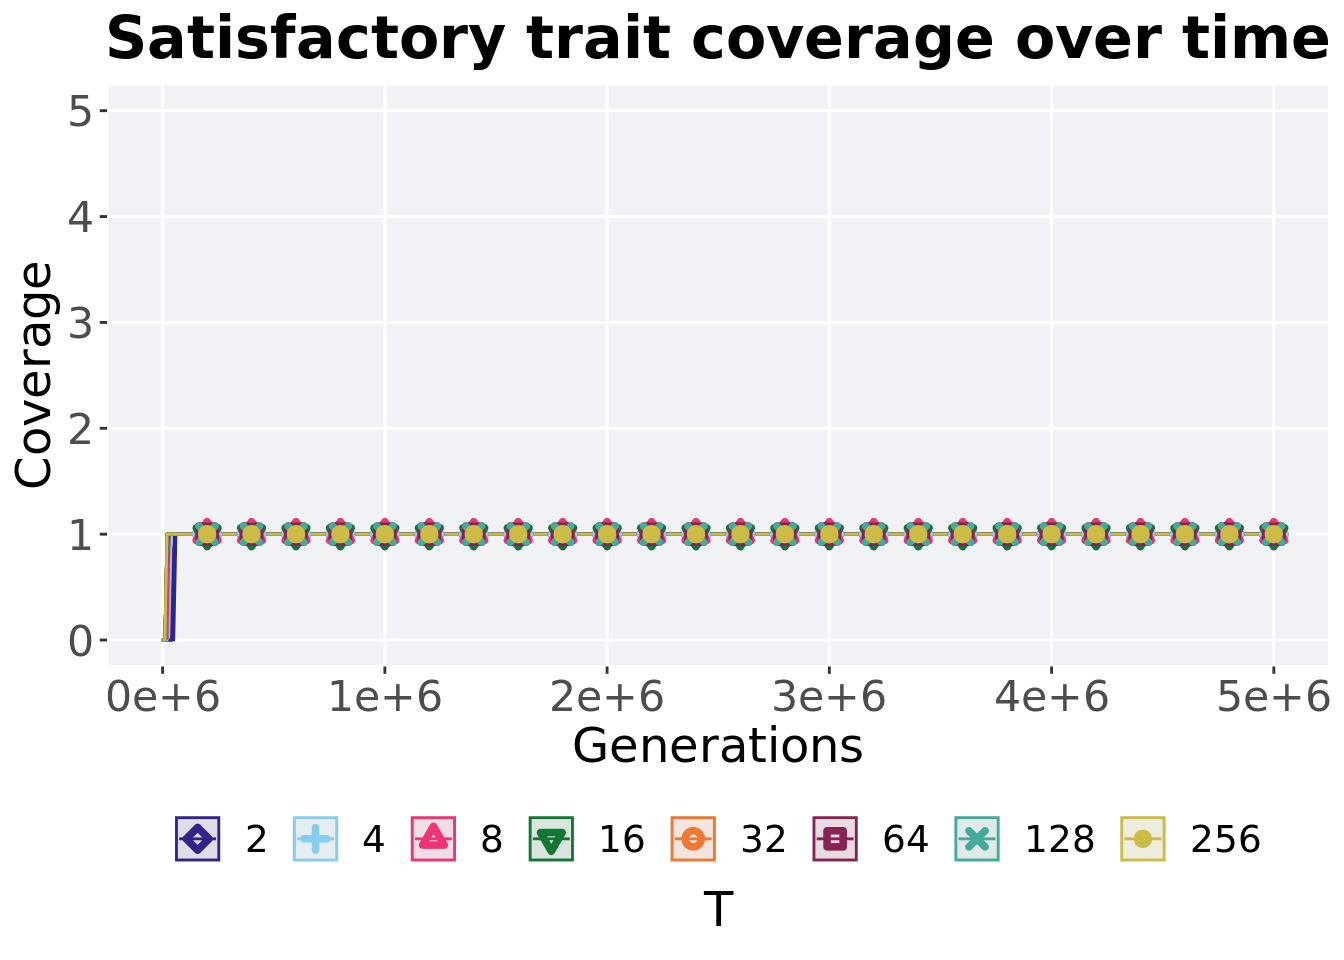
\includegraphics{demo_files/figure-latex/unnamed-chunk-120-1.pdf}

\hypertarget{best-coverage-throughout-3}{%
\subsubsection{Best coverage throughout}\label{best-coverage-throughout-3}}

Best satisfactory trait coverage throughout 50,000 generations.

\begin{Shaded}
\begin{Highlighting}[]
\NormalTok{best =}\StringTok{ }\KeywordTok{filter}\NormalTok{(tor_best, col }\OperatorTok{==}\StringTok{ 'pop_uni_obj'} \OperatorTok{&}\StringTok{ }\NormalTok{diagnostic }\OperatorTok{==}\StringTok{ 'contradictory_objectives'}\NormalTok{)}

\NormalTok{plot =}\StringTok{ }\KeywordTok{ggplot}\NormalTok{(best, }\KeywordTok{aes}\NormalTok{(}\DataTypeTok{x =}\NormalTok{ T, }\DataTypeTok{y =}\NormalTok{ val, }\DataTypeTok{color =}\NormalTok{ T, }\DataTypeTok{fill =}\NormalTok{ T, }\DataTypeTok{shape =}\NormalTok{ T)) }\OperatorTok{+}
\StringTok{  }\KeywordTok{geom_flat_violin}\NormalTok{(}\DataTypeTok{position =} \KeywordTok{position_nudge}\NormalTok{(}\DataTypeTok{x =} \FloatTok{.2}\NormalTok{, }\DataTypeTok{y =} \DecValTok{0}\NormalTok{), }\DataTypeTok{scale =} \StringTok{'width'}\NormalTok{, }\DataTypeTok{alpha =} \FloatTok{0.2}\NormalTok{) }\OperatorTok{+}
\StringTok{  }\KeywordTok{geom_point}\NormalTok{(}\DataTypeTok{position =} \KeywordTok{position_jitter}\NormalTok{(}\DataTypeTok{width =} \FloatTok{.1}\NormalTok{), }\DataTypeTok{size =} \FloatTok{1.5}\NormalTok{, }\DataTypeTok{alpha =} \FloatTok{1.0}\NormalTok{) }\OperatorTok{+}
\StringTok{  }\KeywordTok{geom_boxplot}\NormalTok{(}\DataTypeTok{color =} \StringTok{'black'}\NormalTok{, }\DataTypeTok{width =} \FloatTok{.2}\NormalTok{, }\DataTypeTok{outlier.shape =} \OtherTok{NA}\NormalTok{, }\DataTypeTok{alpha =} \FloatTok{0.0}\NormalTok{) }\OperatorTok{+}
\StringTok{  }\KeywordTok{scale_y_continuous}\NormalTok{(}
    \DataTypeTok{name=}\StringTok{"Coverage"}\NormalTok{,}
    \DataTypeTok{limits=}\KeywordTok{c}\NormalTok{(}\DecValTok{0}\NormalTok{, }\DecValTok{5}\NormalTok{)}
\NormalTok{  ) }\OperatorTok{+}
\StringTok{  }\KeywordTok{scale_x_discrete}\NormalTok{(}
    \DataTypeTok{name=}\StringTok{"T"}
\NormalTok{  )}\OperatorTok{+}
\StringTok{  }\KeywordTok{scale_shape_manual}\NormalTok{(}\DataTypeTok{values=}\NormalTok{SHAPE)}\OperatorTok{+}
\StringTok{  }\KeywordTok{scale_colour_manual}\NormalTok{(}\DataTypeTok{values =}\NormalTok{ cb_palette) }\OperatorTok{+}
\StringTok{  }\KeywordTok{scale_fill_manual}\NormalTok{(}\DataTypeTok{values =}\NormalTok{ cb_palette) }\OperatorTok{+}
\StringTok{  }\NormalTok{p_theme}

\KeywordTok{plot_grid}\NormalTok{(}
\NormalTok{  plot }\OperatorTok{+}
\StringTok{    }\KeywordTok{ggtitle}\NormalTok{(}\StringTok{"Best satisfactory trait coverage"}\NormalTok{) }\OperatorTok{+}
\StringTok{    }\KeywordTok{theme}\NormalTok{(}\DataTypeTok{legend.position=}\StringTok{"none"}\NormalTok{),}
\NormalTok{  legend,}
  \DataTypeTok{nrow=}\DecValTok{2}\NormalTok{,}
  \DataTypeTok{rel_heights =} \KeywordTok{c}\NormalTok{(}\DecValTok{2}\NormalTok{,.}\DecValTok{2}\NormalTok{),}
  \DataTypeTok{label_size =}\NormalTok{ TSIZE}
\NormalTok{)}
\end{Highlighting}
\end{Shaded}

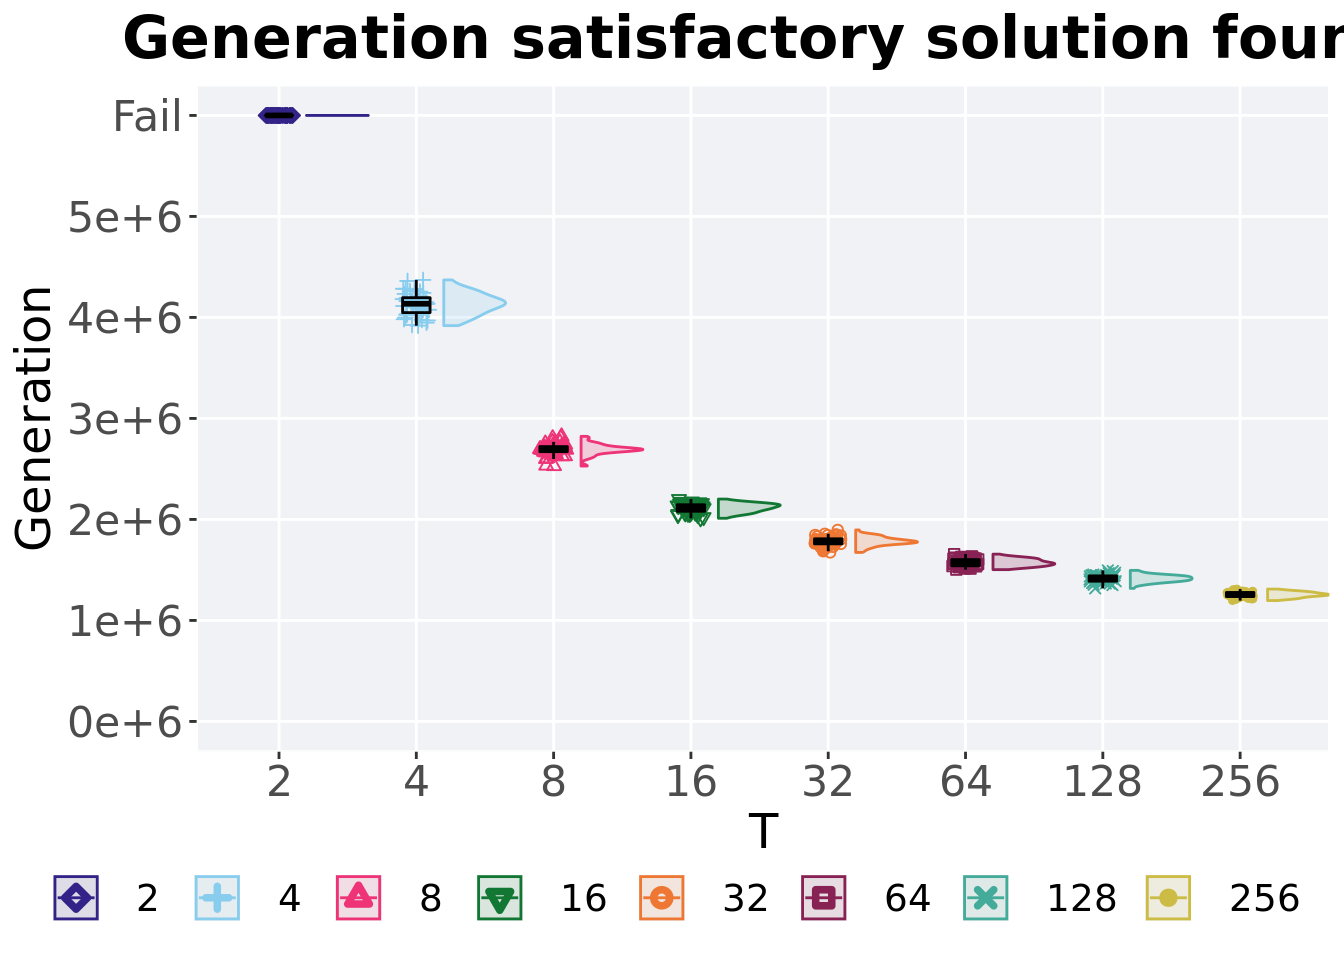
\includegraphics{demo_files/figure-latex/unnamed-chunk-122-1.pdf}

\hypertarget{stats-22}{%
\paragraph{Stats}\label{stats-22}}

Summary statistics for the best satisfactory trait coverage throughout 50,000 generations.

\begin{Shaded}
\begin{Highlighting}[]
\KeywordTok{group_by}\NormalTok{(best, T) }\OperatorTok
\StringTok{  }\NormalTok{dplyr}\OperatorTok{::}\KeywordTok{summarise}\NormalTok{(}
    \DataTypeTok{count =} \KeywordTok{n}\NormalTok{(),}
    \DataTypeTok{na_cnt =} \KeywordTok{sum}\NormalTok{(}\KeywordTok{is.na}\NormalTok{(val)),}
    \DataTypeTok{min =} \KeywordTok{min}\NormalTok{(val, }\DataTypeTok{na.rm =} \OtherTok{TRUE}\NormalTok{),}
    \DataTypeTok{median =} \KeywordTok{median}\NormalTok{(val, }\DataTypeTok{na.rm =} \OtherTok{TRUE}\NormalTok{),}
    \DataTypeTok{mean =} \KeywordTok{mean}\NormalTok{(val, }\DataTypeTok{na.rm =} \OtherTok{TRUE}\NormalTok{),}
    \DataTypeTok{max =} \KeywordTok{max}\NormalTok{(val, }\DataTypeTok{na.rm =} \OtherTok{TRUE}\NormalTok{),}
    \DataTypeTok{IQR =} \KeywordTok{IQR}\NormalTok{(val, }\DataTypeTok{na.rm =} \OtherTok{TRUE}\NormalTok{)}
\NormalTok{  )}
\end{Highlighting}
\end{Shaded}

\begin{verbatim}
## # A tibble: 8 x 8
##   T     count na_cnt   min median  mean   max   IQR
##   <fct> <int>  <int> <dbl>  <dbl> <dbl> <dbl> <dbl>
## 1 2        50      0     1      1     1     1     0
## 2 4        50      0     1      1     1     1     0
## 3 8        50      0     1      1     1     1     0
## 4 16       50      0     1      1     1     1     0
## 5 32       50      0     1      1     1     1     0
## 6 64       50      0     1      1     1     1     0
## 7 128      50      0     1      1     1     1     0
## 8 256      50      0     1      1     1     1     0
\end{verbatim}

\hypertarget{end-of-50000-generations-9}{%
\subsubsection{End of 50,000 generations}\label{end-of-50000-generations-9}}

Satisfactory trait coverage in the population at the end of 50,000 generations.

\begin{Shaded}
\begin{Highlighting}[]
\NormalTok{end =}\StringTok{ }\KeywordTok{filter}\NormalTok{(tor_end, diagnostic }\OperatorTok{==}\StringTok{ 'contradictory_objectives'}\NormalTok{)}
\NormalTok{plot =}\StringTok{ }\KeywordTok{ggplot}\NormalTok{(end, }\KeywordTok{aes}\NormalTok{(}\DataTypeTok{x =}\NormalTok{ T, }\DataTypeTok{y =}\NormalTok{ pop_uni_obj, }\DataTypeTok{color =}\NormalTok{ T, }\DataTypeTok{fill =}\NormalTok{ T, }\DataTypeTok{shape =}\NormalTok{ T)) }\OperatorTok{+}
\StringTok{  }\KeywordTok{geom_flat_violin}\NormalTok{(}\DataTypeTok{position =} \KeywordTok{position_nudge}\NormalTok{(}\DataTypeTok{x =} \FloatTok{.2}\NormalTok{, }\DataTypeTok{y =} \DecValTok{0}\NormalTok{), }\DataTypeTok{scale =} \StringTok{'width'}\NormalTok{, }\DataTypeTok{alpha =} \FloatTok{0.2}\NormalTok{) }\OperatorTok{+}
\StringTok{  }\KeywordTok{geom_point}\NormalTok{(}\DataTypeTok{position =} \KeywordTok{position_jitter}\NormalTok{(}\DataTypeTok{width =} \FloatTok{.1}\NormalTok{), }\DataTypeTok{size =} \FloatTok{1.5}\NormalTok{, }\DataTypeTok{alpha =} \FloatTok{1.0}\NormalTok{) }\OperatorTok{+}
\StringTok{  }\KeywordTok{geom_boxplot}\NormalTok{(}\DataTypeTok{color =} \StringTok{'black'}\NormalTok{, }\DataTypeTok{width =} \FloatTok{.2}\NormalTok{, }\DataTypeTok{outlier.shape =} \OtherTok{NA}\NormalTok{, }\DataTypeTok{alpha =} \FloatTok{0.0}\NormalTok{) }\OperatorTok{+}
\StringTok{  }\KeywordTok{scale_y_continuous}\NormalTok{(}
    \DataTypeTok{name=}\StringTok{"Coverage"}\NormalTok{,}
    \DataTypeTok{limits=}\KeywordTok{c}\NormalTok{(}\DecValTok{0}\NormalTok{, }\DecValTok{5}\NormalTok{)}
\NormalTok{  ) }\OperatorTok{+}
\StringTok{  }\KeywordTok{scale_x_discrete}\NormalTok{(}
    \DataTypeTok{name=}\StringTok{"T"}
\NormalTok{  )}\OperatorTok{+}
\StringTok{  }\KeywordTok{scale_shape_manual}\NormalTok{(}\DataTypeTok{values=}\NormalTok{SHAPE)}\OperatorTok{+}
\StringTok{  }\KeywordTok{scale_colour_manual}\NormalTok{(}\DataTypeTok{values =}\NormalTok{ cb_palette) }\OperatorTok{+}
\StringTok{  }\KeywordTok{scale_fill_manual}\NormalTok{(}\DataTypeTok{values =}\NormalTok{ cb_palette) }\OperatorTok{+}
\StringTok{  }\NormalTok{p_theme}

\KeywordTok{plot_grid}\NormalTok{(}
\NormalTok{  plot }\OperatorTok{+}
\StringTok{    }\KeywordTok{ggtitle}\NormalTok{(}\StringTok{"Final satisfactory trait coverage"}\NormalTok{) }\OperatorTok{+}
\StringTok{    }\KeywordTok{theme}\NormalTok{(}\DataTypeTok{legend.position=}\StringTok{"none"}\NormalTok{),}
\NormalTok{  legend,}
  \DataTypeTok{nrow=}\DecValTok{2}\NormalTok{,}
  \DataTypeTok{rel_heights =} \KeywordTok{c}\NormalTok{(}\DecValTok{2}\NormalTok{,.}\DecValTok{3}\NormalTok{),}
  \DataTypeTok{label_size =}\NormalTok{ TSIZE}
\NormalTok{)}
\end{Highlighting}
\end{Shaded}

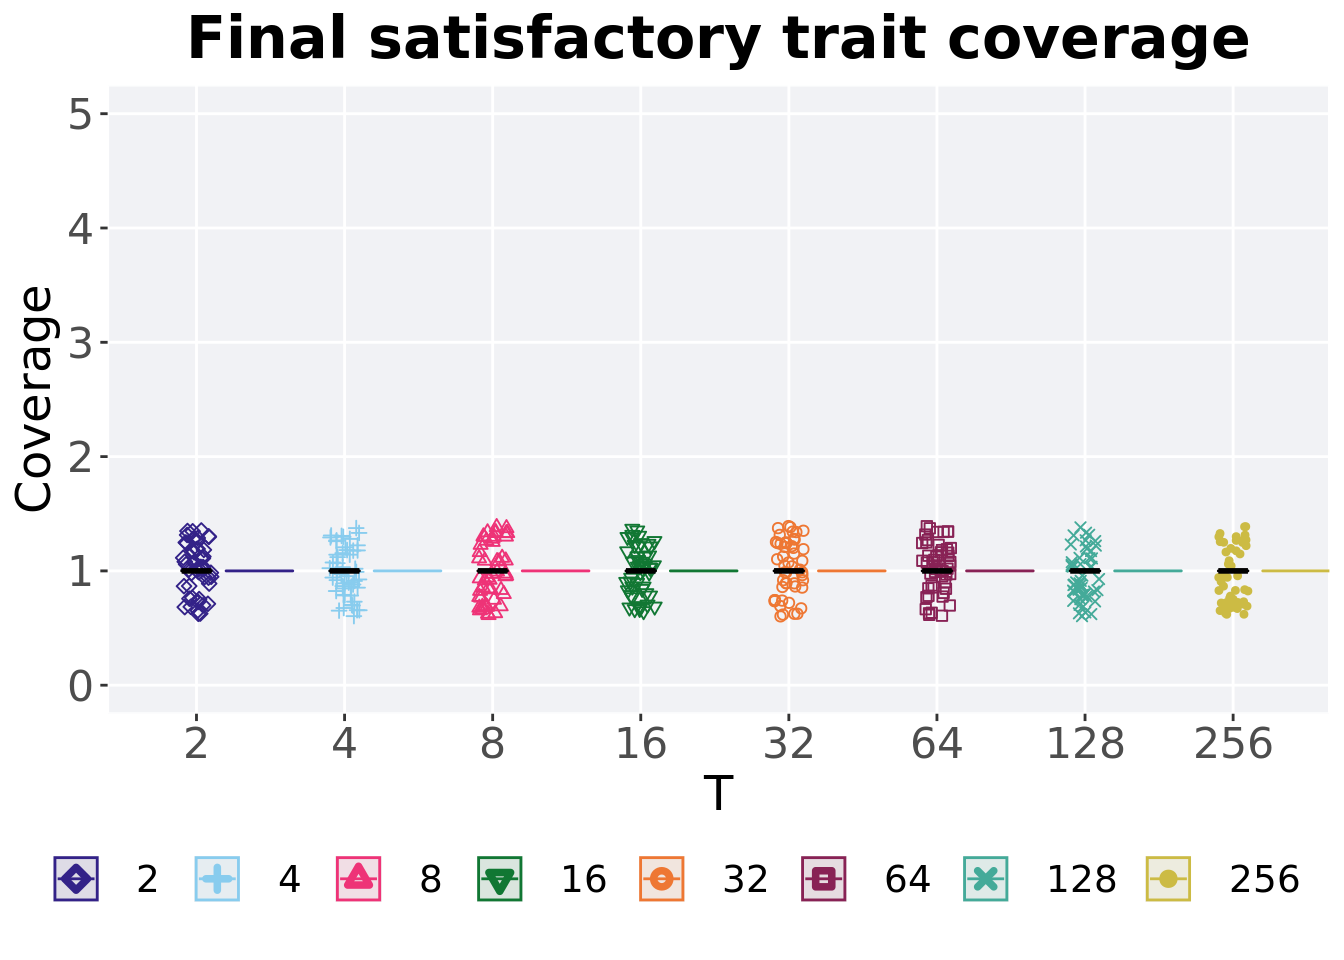
\includegraphics{demo_files/figure-latex/unnamed-chunk-124-1.pdf}

\hypertarget{stats-23}{%
\paragraph{Stats}\label{stats-23}}

Summary statistics for satisfactory trait coverage in the population at the end of 50,000 generations.

\begin{Shaded}
\begin{Highlighting}[]
\KeywordTok{group_by}\NormalTok{(end, T) }\OperatorTok
\StringTok{  }\NormalTok{dplyr}\OperatorTok{::}\KeywordTok{summarise}\NormalTok{(}
    \DataTypeTok{count =} \KeywordTok{n}\NormalTok{(),}
    \DataTypeTok{na_cnt =} \KeywordTok{sum}\NormalTok{(}\KeywordTok{is.na}\NormalTok{(pop_uni_obj)),}
    \DataTypeTok{min =} \KeywordTok{min}\NormalTok{(pop_uni_obj, }\DataTypeTok{na.rm =} \OtherTok{TRUE}\NormalTok{),}
    \DataTypeTok{median =} \KeywordTok{median}\NormalTok{(pop_uni_obj, }\DataTypeTok{na.rm =} \OtherTok{TRUE}\NormalTok{),}
    \DataTypeTok{mean =} \KeywordTok{mean}\NormalTok{(pop_uni_obj, }\DataTypeTok{na.rm =} \OtherTok{TRUE}\NormalTok{),}
    \DataTypeTok{max =} \KeywordTok{max}\NormalTok{(pop_uni_obj, }\DataTypeTok{na.rm =} \OtherTok{TRUE}\NormalTok{),}
    \DataTypeTok{IQR =} \KeywordTok{IQR}\NormalTok{(pop_uni_obj, }\DataTypeTok{na.rm =} \OtherTok{TRUE}\NormalTok{)}
\NormalTok{  )}
\end{Highlighting}
\end{Shaded}

\begin{verbatim}
## # A tibble: 8 x 8
##   T     count na_cnt   min median  mean   max   IQR
##   <fct> <int>  <int> <int>  <dbl> <dbl> <int> <dbl>
## 1 2        50      0     1      1     1     1     0
## 2 4        50      0     1      1     1     1     0
## 3 8        50      0     1      1     1     1     0
## 4 16       50      0     1      1     1     1     0
## 5 32       50      0     1      1     1     1     0
## 6 64       50      0     1      1     1     1     0
## 7 128      50      0     1      1     1     1     0
## 8 256      50      0     1      1     1     1     0
\end{verbatim}

\hypertarget{activation-gene-coverage-4}{%
\subsection{Activation gene coverage}\label{activation-gene-coverage-4}}

Here we analyze the activation gene coverage for each parameter replicate on the contradictory objectives diagnostic.

\hypertarget{coverage-over-time-6}{%
\subsubsection{Coverage over time}\label{coverage-over-time-6}}

Activation gene coverage over time.

\begin{Shaded}
\begin{Highlighting}[]
\NormalTok{problem <-}\StringTok{ }\KeywordTok{filter}\NormalTok{(tor_ot, diagnostic }\OperatorTok{==}\StringTok{ 'contradictory_objectives'}\NormalTok{)}
\NormalTok{lines =}\StringTok{ }\NormalTok{problem }\OperatorTok
\StringTok{        }\KeywordTok{group_by}\NormalTok{(T, gen) }\OperatorTok
\StringTok{          }\NormalTok{dplyr}\OperatorTok{::}\KeywordTok{summarise}\NormalTok{(}
            \DataTypeTok{min =} \KeywordTok{min}\NormalTok{(uni_str_pos),}
            \DataTypeTok{mean =} \KeywordTok{mean}\NormalTok{(uni_str_pos),}
            \DataTypeTok{max =} \KeywordTok{max}\NormalTok{(uni_str_pos)}
\NormalTok{          )}
\end{Highlighting}
\end{Shaded}

\begin{verbatim}
## `summarise()` has grouped output by 'T'. You can override using the `.groups`
## argument.
\end{verbatim}

\begin{Shaded}
\begin{Highlighting}[]
\NormalTok{points =}\StringTok{ }\KeywordTok{filter}\NormalTok{(lines, gen }\OperatorTok\StringTok{ }\DecValTok{2000} \OperatorTok{==}\StringTok{ }\DecValTok{0} \OperatorTok{&}\StringTok{ }\NormalTok{gen }\OperatorTok{!=}\StringTok{ }\DecValTok{0}\NormalTok{)}

\NormalTok{ot =}\StringTok{ }\KeywordTok{ggplot}\NormalTok{(lines, }\KeywordTok{aes}\NormalTok{(}\DataTypeTok{x=}\NormalTok{gen, }\DataTypeTok{y=}\NormalTok{mean, }\DataTypeTok{group =}\NormalTok{ T, }\DataTypeTok{fill =}\NormalTok{T, }\DataTypeTok{color =}\NormalTok{ T, }\DataTypeTok{shape =}\NormalTok{ T)) }\OperatorTok{+}
\StringTok{  }\KeywordTok{geom_ribbon}\NormalTok{(}\KeywordTok{aes}\NormalTok{(}\DataTypeTok{ymin =}\NormalTok{ min, }\DataTypeTok{ymax =}\NormalTok{ max), }\DataTypeTok{alpha =} \FloatTok{0.1}\NormalTok{) }\OperatorTok{+}
\StringTok{  }\KeywordTok{geom_line}\NormalTok{(}\DataTypeTok{size =} \FloatTok{0.5}\NormalTok{) }\OperatorTok{+}
\StringTok{  }\KeywordTok{geom_point}\NormalTok{(}\DataTypeTok{data =}\NormalTok{ points, }\DataTypeTok{size =} \FloatTok{1.5}\NormalTok{, }\DataTypeTok{stroke =} \FloatTok{2.0}\NormalTok{, }\DataTypeTok{alpha =} \FloatTok{1.0}\NormalTok{) }\OperatorTok{+}
\StringTok{  }\KeywordTok{scale_y_continuous}\NormalTok{(}
    \DataTypeTok{name=}\StringTok{"Coverage"}\NormalTok{,}
    \DataTypeTok{limits=}\KeywordTok{c}\NormalTok{(}\OperatorTok{-}\DecValTok{1}\NormalTok{, }\DecValTok{101}\NormalTok{),}
    \DataTypeTok{breaks=}\KeywordTok{seq}\NormalTok{(}\DecValTok{0}\NormalTok{,}\DecValTok{100}\NormalTok{, }\DecValTok{20}\NormalTok{),}
    \DataTypeTok{labels=}\KeywordTok{c}\NormalTok{(}\StringTok{"0"}\NormalTok{, }\StringTok{"20"}\NormalTok{, }\StringTok{"40"}\NormalTok{, }\StringTok{"60"}\NormalTok{, }\StringTok{"80"}\NormalTok{, }\StringTok{"100"}\NormalTok{)}
\NormalTok{  ) }\OperatorTok{+}
\StringTok{  }\KeywordTok{scale_x_continuous}\NormalTok{(}
    \DataTypeTok{name=}\StringTok{"Generations"}\NormalTok{,}
    \DataTypeTok{limits=}\KeywordTok{c}\NormalTok{(}\DecValTok{0}\NormalTok{, }\DecValTok{50000}\NormalTok{),}
    \DataTypeTok{breaks=}\KeywordTok{c}\NormalTok{(}\DecValTok{0}\NormalTok{, }\DecValTok{10000}\NormalTok{, }\DecValTok{20000}\NormalTok{, }\DecValTok{30000}\NormalTok{, }\DecValTok{40000}\NormalTok{, }\DecValTok{50000}\NormalTok{),}
    \DataTypeTok{labels=}\KeywordTok{c}\NormalTok{(}\StringTok{"0e+6"}\NormalTok{, }\StringTok{"1e+6"}\NormalTok{, }\StringTok{"2e+6"}\NormalTok{, }\StringTok{"3e+6"}\NormalTok{, }\StringTok{"4e+6"}\NormalTok{, }\StringTok{"5e+6"}\NormalTok{)}

\NormalTok{  ) }\OperatorTok{+}
\StringTok{  }\KeywordTok{scale_shape_manual}\NormalTok{(}\DataTypeTok{values=}\NormalTok{SHAPE)}\OperatorTok{+}
\StringTok{  }\KeywordTok{scale_colour_manual}\NormalTok{(}\DataTypeTok{values =}\NormalTok{ cb_palette) }\OperatorTok{+}
\StringTok{  }\KeywordTok{scale_fill_manual}\NormalTok{(}\DataTypeTok{values =}\NormalTok{ cb_palette) }\OperatorTok{+}
\StringTok{  }\KeywordTok{ggtitle}\NormalTok{(}\StringTok{"Activation gene coverage over time"}\NormalTok{) }\OperatorTok{+}
\StringTok{  }\NormalTok{p_theme}\OperatorTok{+}
\StringTok{    }\KeywordTok{guides}\NormalTok{(}
    \DataTypeTok{shape=}\KeywordTok{guide_legend}\NormalTok{(}\DataTypeTok{nrow=}\DecValTok{1}\NormalTok{, }\DataTypeTok{title.position =} \StringTok{"bottom"}\NormalTok{),}
    \DataTypeTok{color=}\KeywordTok{guide_legend}\NormalTok{(}\DataTypeTok{nrow=}\DecValTok{1}\NormalTok{, }\DataTypeTok{title.position =} \StringTok{"bottom"}\NormalTok{),}
    \DataTypeTok{fill=}\KeywordTok{guide_legend}\NormalTok{(}\DataTypeTok{nrow=}\DecValTok{1}\NormalTok{, }\DataTypeTok{title.position =} \StringTok{"bottom"}\NormalTok{)}
\NormalTok{  ) }\OperatorTok{+}
\StringTok{  }\KeywordTok{theme}\NormalTok{(}
    \DataTypeTok{legend.position =} \StringTok{"bottom"}\NormalTok{,}
    \DataTypeTok{legend.box=}\StringTok{"verticle"}\NormalTok{,}
    \DataTypeTok{legend.justification=}\StringTok{"center"}\NormalTok{,}
    \DataTypeTok{legend.title.align=}\FloatTok{0.5}
\NormalTok{  )}

\NormalTok{ot}
\end{Highlighting}
\end{Shaded}

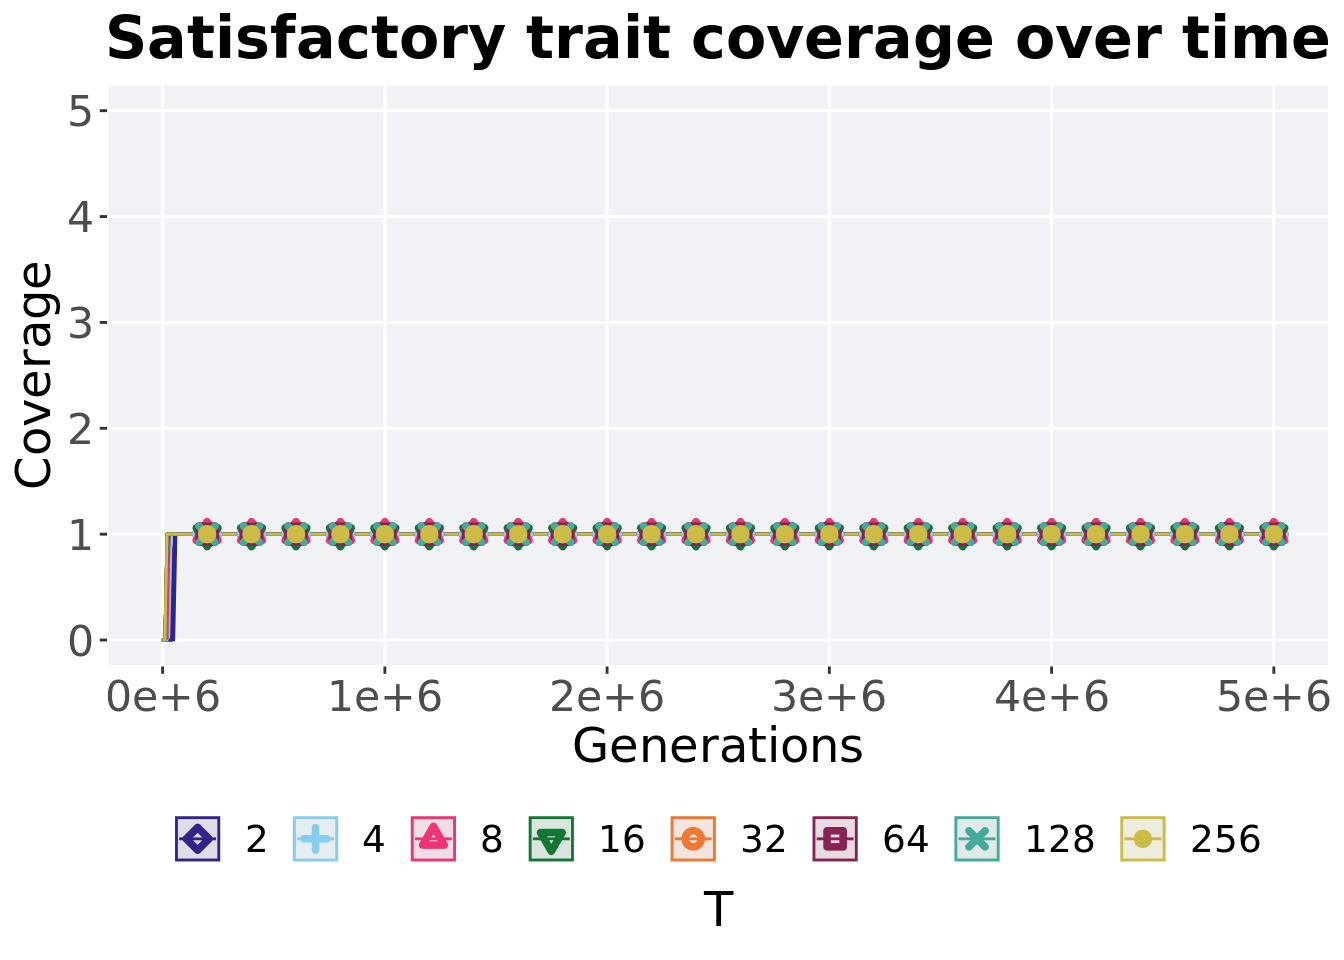
\includegraphics{demo_files/figure-latex/unnamed-chunk-126-1.pdf}

\hypertarget{end-of-50000-generations-10}{%
\subsubsection{End of 50,000 generations}\label{end-of-50000-generations-10}}

Activation gene coverage in the population at the end of 50,000 generations.

\begin{Shaded}
\begin{Highlighting}[]
\NormalTok{end =}\StringTok{ }\KeywordTok{filter}\NormalTok{(tor_end, diagnostic }\OperatorTok{==}\StringTok{ 'contradictory_objectives'}\NormalTok{)}
\NormalTok{plot =}\StringTok{ }\KeywordTok{ggplot}\NormalTok{(end, }\KeywordTok{aes}\NormalTok{(}\DataTypeTok{x =}\NormalTok{ T, }\DataTypeTok{y =}\NormalTok{ uni_str_pos, }\DataTypeTok{color =}\NormalTok{ T, }\DataTypeTok{fill =}\NormalTok{ T, }\DataTypeTok{shape =}\NormalTok{ T)) }\OperatorTok{+}
\StringTok{  }\KeywordTok{geom_flat_violin}\NormalTok{(}\DataTypeTok{position =} \KeywordTok{position_nudge}\NormalTok{(}\DataTypeTok{x =} \FloatTok{.2}\NormalTok{, }\DataTypeTok{y =} \DecValTok{0}\NormalTok{), }\DataTypeTok{scale =} \StringTok{'width'}\NormalTok{, }\DataTypeTok{alpha =} \FloatTok{0.2}\NormalTok{) }\OperatorTok{+}
\StringTok{  }\KeywordTok{geom_point}\NormalTok{(}\DataTypeTok{position =} \KeywordTok{position_jitter}\NormalTok{(}\DataTypeTok{width =} \FloatTok{.1}\NormalTok{), }\DataTypeTok{size =} \FloatTok{1.5}\NormalTok{, }\DataTypeTok{alpha =} \FloatTok{1.0}\NormalTok{) }\OperatorTok{+}
\StringTok{  }\KeywordTok{geom_boxplot}\NormalTok{(}\DataTypeTok{color =} \StringTok{'black'}\NormalTok{, }\DataTypeTok{width =} \FloatTok{.2}\NormalTok{, }\DataTypeTok{outlier.shape =} \OtherTok{NA}\NormalTok{, }\DataTypeTok{alpha =} \FloatTok{0.0}\NormalTok{) }\OperatorTok{+}
\StringTok{  }\KeywordTok{scale_y_continuous}\NormalTok{(}
    \DataTypeTok{name=}\StringTok{"Coverage"}\NormalTok{,}
    \DataTypeTok{limits=}\KeywordTok{c}\NormalTok{(}\DecValTok{0}\NormalTok{, }\DecValTok{5}\NormalTok{)}
\NormalTok{  ) }\OperatorTok{+}
\StringTok{  }\KeywordTok{scale_x_discrete}\NormalTok{(}
    \DataTypeTok{name=}\StringTok{"T"}
\NormalTok{  )}\OperatorTok{+}
\StringTok{  }\KeywordTok{scale_shape_manual}\NormalTok{(}\DataTypeTok{values=}\NormalTok{SHAPE)}\OperatorTok{+}
\StringTok{  }\KeywordTok{scale_colour_manual}\NormalTok{(}\DataTypeTok{values =}\NormalTok{ cb_palette) }\OperatorTok{+}
\StringTok{  }\KeywordTok{scale_fill_manual}\NormalTok{(}\DataTypeTok{values =}\NormalTok{ cb_palette) }\OperatorTok{+}
\StringTok{  }\NormalTok{p_theme}

\KeywordTok{plot_grid}\NormalTok{(}
\NormalTok{  plot }\OperatorTok{+}
\StringTok{    }\KeywordTok{ggtitle}\NormalTok{(}\StringTok{"Final activation gene coverage"}\NormalTok{) }\OperatorTok{+}
\StringTok{    }\KeywordTok{theme}\NormalTok{(}\DataTypeTok{legend.position=}\StringTok{"none"}\NormalTok{),}
\NormalTok{  legend,}
  \DataTypeTok{nrow=}\DecValTok{2}\NormalTok{,}
  \DataTypeTok{rel_heights =} \KeywordTok{c}\NormalTok{(}\DecValTok{2}\NormalTok{,.}\DecValTok{2}\NormalTok{),}
  \DataTypeTok{label_size =}\NormalTok{ TSIZE}
\NormalTok{)}
\end{Highlighting}
\end{Shaded}

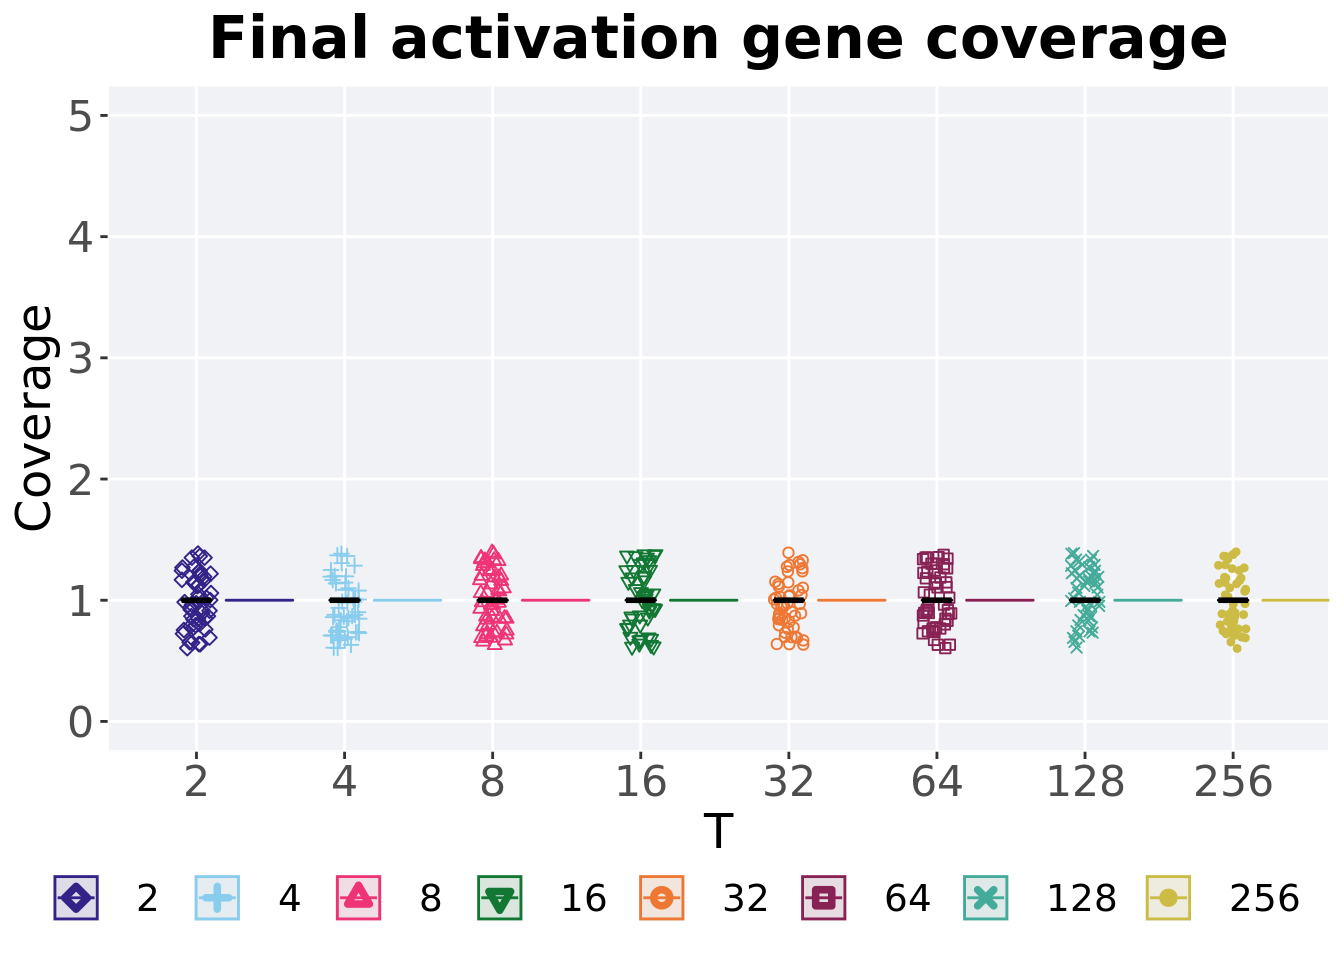
\includegraphics{demo_files/figure-latex/unnamed-chunk-127-1.pdf}

\hypertarget{stats-24}{%
\paragraph{Stats}\label{stats-24}}

Summary statistics for activation gene coverage in the population at the end of 50,000 generations.

\begin{Shaded}
\begin{Highlighting}[]
\KeywordTok{group_by}\NormalTok{(end, T) }\OperatorTok
\StringTok{  }\NormalTok{dplyr}\OperatorTok{::}\KeywordTok{summarise}\NormalTok{(}
    \DataTypeTok{count =} \KeywordTok{n}\NormalTok{(),}
    \DataTypeTok{na_cnt =} \KeywordTok{sum}\NormalTok{(}\KeywordTok{is.na}\NormalTok{(uni_str_pos)),}
    \DataTypeTok{min =} \KeywordTok{min}\NormalTok{(uni_str_pos, }\DataTypeTok{na.rm =} \OtherTok{TRUE}\NormalTok{),}
    \DataTypeTok{median =} \KeywordTok{median}\NormalTok{(uni_str_pos, }\DataTypeTok{na.rm =} \OtherTok{TRUE}\NormalTok{),}
    \DataTypeTok{mean =} \KeywordTok{mean}\NormalTok{(uni_str_pos, }\DataTypeTok{na.rm =} \OtherTok{TRUE}\NormalTok{),}
    \DataTypeTok{max =} \KeywordTok{max}\NormalTok{(uni_str_pos, }\DataTypeTok{na.rm =} \OtherTok{TRUE}\NormalTok{),}
    \DataTypeTok{IQR =} \KeywordTok{IQR}\NormalTok{(uni_str_pos, }\DataTypeTok{na.rm =} \OtherTok{TRUE}\NormalTok{)}
\NormalTok{  )}
\end{Highlighting}
\end{Shaded}

\begin{verbatim}
## # A tibble: 8 x 8
##   T     count na_cnt   min median  mean   max   IQR
##   <fct> <int>  <int> <int>  <dbl> <dbl> <int> <dbl>
## 1 2        50      0     1      1     1     1     0
## 2 4        50      0     1      1     1     1     0
## 3 8        50      0     1      1     1     1     0
## 4 16       50      0     1      1     1     1     0
## 5 32       50      0     1      1     1     1     0
## 6 64       50      0     1      1     1     1     0
## 7 128      50      0     1      1     1     1     0
## 8 256      50      0     1      1     1     1     0
\end{verbatim}

\hypertarget{multi-path-exploration-results-2}{%
\section{Multi-path exploration results}\label{multi-path-exploration-results-2}}

Here we present the results for \textbf{best performances} and \textbf{activation gene coverage} found by each genotypic fitness sharing sigma value replicate on the multi-path exploration diagnostic.
Best performance found refers to the largest average trait score found in a given population, while activation gene coverage refers to the count of unique activation genes in the population.
Note that both values fall between 0 and 100.

\hypertarget{performance-2}{%
\subsection{Performance}\label{performance-2}}

Here we analyze the performances for each parameter replicate on the multi-path exploration diagnostic.

\hypertarget{performance-over-time-7}{%
\subsubsection{Performance over time}\label{performance-over-time-7}}

Performance over time.

\begin{Shaded}
\begin{Highlighting}[]
\NormalTok{problem <-}\StringTok{ }\KeywordTok{filter}\NormalTok{(tor_ot, diagnostic }\OperatorTok{==}\StringTok{ 'multipath_exploration'}\NormalTok{)}
\NormalTok{lines =}\StringTok{ }\NormalTok{problem }\OperatorTok
\StringTok{        }\KeywordTok{group_by}\NormalTok{(T, gen) }\OperatorTok
\StringTok{          }\NormalTok{dplyr}\OperatorTok{::}\KeywordTok{summarise}\NormalTok{(}
            \DataTypeTok{min =} \KeywordTok{min}\NormalTok{(pop_fit_max),}
            \DataTypeTok{mean =} \KeywordTok{mean}\NormalTok{(pop_fit_max),}
            \DataTypeTok{max =} \KeywordTok{max}\NormalTok{(pop_fit_max)}
\NormalTok{          )}
\end{Highlighting}
\end{Shaded}

\begin{verbatim}
## `summarise()` has grouped output by 'T'. You can override using the `.groups`
## argument.
\end{verbatim}

\begin{Shaded}
\begin{Highlighting}[]
\NormalTok{points =}\StringTok{ }\KeywordTok{filter}\NormalTok{(lines, gen }\OperatorTok\StringTok{ }\DecValTok{2000} \OperatorTok{==}\StringTok{ }\DecValTok{0} \OperatorTok{&}\StringTok{ }\NormalTok{gen }\OperatorTok{!=}\StringTok{ }\DecValTok{0}\NormalTok{)}

\NormalTok{ot =}\StringTok{ }\KeywordTok{ggplot}\NormalTok{(lines, }\KeywordTok{aes}\NormalTok{(}\DataTypeTok{x=}\NormalTok{gen, }\DataTypeTok{y=}\NormalTok{mean }\OperatorTok{/}\StringTok{ }\NormalTok{TRAITS, }\DataTypeTok{group =}\NormalTok{ T, }\DataTypeTok{fill =}\NormalTok{ T, }\DataTypeTok{color =}\NormalTok{ T, }\DataTypeTok{shape =}\NormalTok{ T)) }\OperatorTok{+}
\StringTok{  }\KeywordTok{geom_ribbon}\NormalTok{(}\KeywordTok{aes}\NormalTok{(}\DataTypeTok{ymin =}\NormalTok{ min }\OperatorTok{/}\StringTok{ }\NormalTok{TRAITS, }\DataTypeTok{ymax =}\NormalTok{ max }\OperatorTok{/}\StringTok{ }\NormalTok{TRAITS), }\DataTypeTok{alpha =} \FloatTok{0.1}\NormalTok{) }\OperatorTok{+}
\StringTok{  }\KeywordTok{geom_line}\NormalTok{(}\DataTypeTok{size =} \FloatTok{0.5}\NormalTok{) }\OperatorTok{+}
\StringTok{  }\KeywordTok{geom_point}\NormalTok{(}\DataTypeTok{data =}\NormalTok{ points, }\DataTypeTok{size =} \FloatTok{1.5}\NormalTok{, }\DataTypeTok{stroke =} \FloatTok{2.0}\NormalTok{, }\DataTypeTok{alpha =} \FloatTok{1.0}\NormalTok{) }\OperatorTok{+}
\StringTok{  }\KeywordTok{scale_y_continuous}\NormalTok{(}
    \DataTypeTok{name=}\StringTok{"Average trait score"}\NormalTok{,}
    \DataTypeTok{limits=}\KeywordTok{c}\NormalTok{(}\OperatorTok{-}\DecValTok{1}\NormalTok{, }\DecValTok{101}\NormalTok{),}
    \DataTypeTok{breaks=}\KeywordTok{seq}\NormalTok{(}\DecValTok{0}\NormalTok{,}\DecValTok{100}\NormalTok{, }\DecValTok{20}\NormalTok{),}
    \DataTypeTok{labels=}\KeywordTok{c}\NormalTok{(}\StringTok{"0"}\NormalTok{, }\StringTok{"20"}\NormalTok{, }\StringTok{"40"}\NormalTok{, }\StringTok{"60"}\NormalTok{, }\StringTok{"80"}\NormalTok{, }\StringTok{"100"}\NormalTok{)}
\NormalTok{  ) }\OperatorTok{+}
\StringTok{  }\KeywordTok{scale_x_continuous}\NormalTok{(}
    \DataTypeTok{name=}\StringTok{"Generations"}\NormalTok{,}
    \DataTypeTok{limits=}\KeywordTok{c}\NormalTok{(}\DecValTok{0}\NormalTok{, }\DecValTok{50000}\NormalTok{),}
    \DataTypeTok{breaks=}\KeywordTok{c}\NormalTok{(}\DecValTok{0}\NormalTok{, }\DecValTok{10000}\NormalTok{, }\DecValTok{20000}\NormalTok{, }\DecValTok{30000}\NormalTok{, }\DecValTok{40000}\NormalTok{, }\DecValTok{50000}\NormalTok{),}
    \DataTypeTok{labels=}\KeywordTok{c}\NormalTok{(}\StringTok{"0e+6"}\NormalTok{, }\StringTok{"1e+6"}\NormalTok{, }\StringTok{"2e+6"}\NormalTok{, }\StringTok{"3e+6"}\NormalTok{, }\StringTok{"4e+6"}\NormalTok{, }\StringTok{"5e+6"}\NormalTok{)}

\NormalTok{  ) }\OperatorTok{+}
\StringTok{  }\KeywordTok{scale_shape_manual}\NormalTok{(}\DataTypeTok{values=}\NormalTok{SHAPE)}\OperatorTok{+}
\StringTok{  }\KeywordTok{scale_colour_manual}\NormalTok{(}\DataTypeTok{values =}\NormalTok{ cb_palette) }\OperatorTok{+}
\StringTok{  }\KeywordTok{scale_fill_manual}\NormalTok{(}\DataTypeTok{values =}\NormalTok{ cb_palette) }\OperatorTok{+}
\StringTok{  }\KeywordTok{ggtitle}\NormalTok{(}\StringTok{"Best performance over time"}\NormalTok{) }\OperatorTok{+}
\StringTok{  }\NormalTok{p_theme}\OperatorTok{+}
\StringTok{    }\KeywordTok{guides}\NormalTok{(}
    \DataTypeTok{shape=}\KeywordTok{guide_legend}\NormalTok{(}\DataTypeTok{nrow=}\DecValTok{1}\NormalTok{, }\DataTypeTok{title.position =} \StringTok{"bottom"}\NormalTok{),}
    \DataTypeTok{color=}\KeywordTok{guide_legend}\NormalTok{(}\DataTypeTok{nrow=}\DecValTok{1}\NormalTok{, }\DataTypeTok{title.position =} \StringTok{"bottom"}\NormalTok{),}
    \DataTypeTok{fill=}\KeywordTok{guide_legend}\NormalTok{(}\DataTypeTok{nrow=}\DecValTok{1}\NormalTok{, }\DataTypeTok{title.position =} \StringTok{"bottom"}\NormalTok{)}
\NormalTok{  ) }\OperatorTok{+}
\StringTok{  }\KeywordTok{theme}\NormalTok{(}
    \DataTypeTok{legend.position =} \StringTok{"bottom"}\NormalTok{,}
    \DataTypeTok{legend.box=}\StringTok{"verticle"}\NormalTok{,}
    \DataTypeTok{legend.justification=}\StringTok{"center"}\NormalTok{,}
    \DataTypeTok{legend.title.align=}\FloatTok{0.5}
\NormalTok{  )}

\NormalTok{ot}
\end{Highlighting}
\end{Shaded}

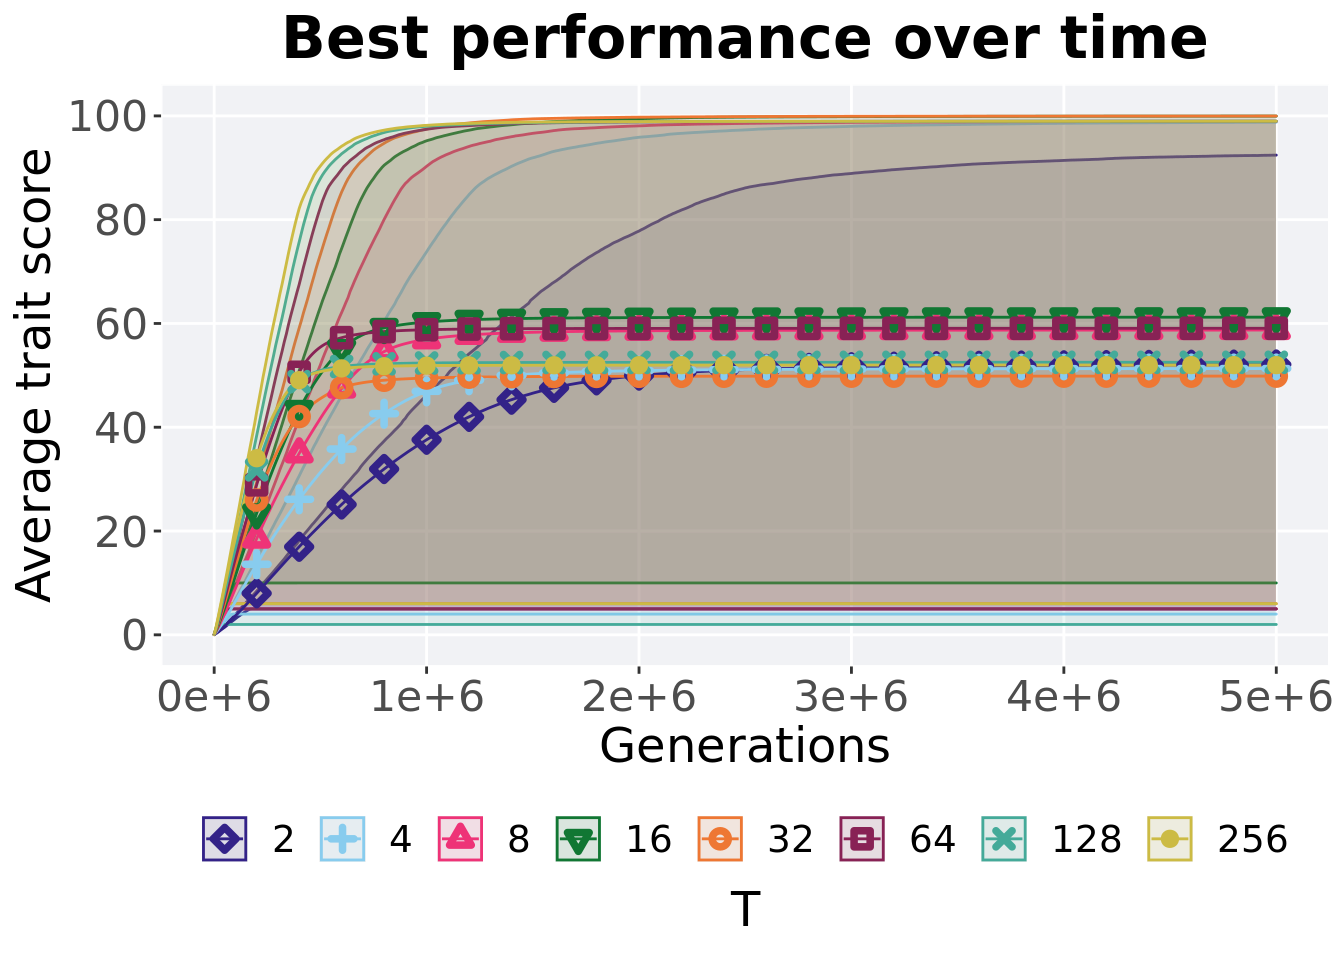
\includegraphics{demo_files/figure-latex/unnamed-chunk-129-1.pdf}

\hypertarget{best-performance-throughout-4}{%
\subsubsection{Best performance throughout}\label{best-performance-throughout-4}}

Here we plot the performance of the best performing solution found throughout 50,000 generations.

\begin{Shaded}
\begin{Highlighting}[]
\NormalTok{best =}\StringTok{ }\KeywordTok{filter}\NormalTok{(tor_best, col }\OperatorTok{==}\StringTok{ 'pop_fit_max'} \OperatorTok{&}\StringTok{ }\NormalTok{diagnostic }\OperatorTok{==}\StringTok{ 'multipath_exploration'}\NormalTok{)}

\NormalTok{plot =}\StringTok{ }\KeywordTok{ggplot}\NormalTok{(best, }\KeywordTok{aes}\NormalTok{(}\DataTypeTok{x =}\NormalTok{ T, }\DataTypeTok{y =}\NormalTok{ val }\OperatorTok{/}\StringTok{ }\NormalTok{TRAITS, }\DataTypeTok{color =}\NormalTok{ T, }\DataTypeTok{fill =}\NormalTok{ T, }\DataTypeTok{shape =}\NormalTok{ T)) }\OperatorTok{+}
\StringTok{  }\KeywordTok{geom_flat_violin}\NormalTok{(}\DataTypeTok{position =} \KeywordTok{position_nudge}\NormalTok{(}\DataTypeTok{x =} \FloatTok{.2}\NormalTok{, }\DataTypeTok{y =} \DecValTok{0}\NormalTok{), }\DataTypeTok{scale =} \StringTok{'width'}\NormalTok{, }\DataTypeTok{alpha =} \FloatTok{0.2}\NormalTok{) }\OperatorTok{+}
\StringTok{  }\KeywordTok{geom_point}\NormalTok{(}\DataTypeTok{position =} \KeywordTok{position_jitter}\NormalTok{(}\DataTypeTok{width =} \FloatTok{.1}\NormalTok{), }\DataTypeTok{size =} \FloatTok{1.5}\NormalTok{, }\DataTypeTok{alpha =} \FloatTok{1.0}\NormalTok{) }\OperatorTok{+}
\StringTok{  }\KeywordTok{geom_boxplot}\NormalTok{(}\DataTypeTok{color =} \StringTok{'black'}\NormalTok{, }\DataTypeTok{width =} \FloatTok{.2}\NormalTok{, }\DataTypeTok{outlier.shape =} \OtherTok{NA}\NormalTok{, }\DataTypeTok{alpha =} \FloatTok{0.0}\NormalTok{) }\OperatorTok{+}
\StringTok{  }\KeywordTok{scale_y_continuous}\NormalTok{(}
    \DataTypeTok{name=}\StringTok{"Average trait score"}\NormalTok{,}
    \DataTypeTok{limits=}\KeywordTok{c}\NormalTok{(}\OperatorTok{-}\DecValTok{1}\NormalTok{, }\DecValTok{101}\NormalTok{),}
    \DataTypeTok{breaks=}\KeywordTok{seq}\NormalTok{(}\DecValTok{0}\NormalTok{,}\DecValTok{100}\NormalTok{, }\DecValTok{20}\NormalTok{),}
    \DataTypeTok{labels=}\KeywordTok{c}\NormalTok{(}\StringTok{"0"}\NormalTok{, }\StringTok{"20"}\NormalTok{, }\StringTok{"40"}\NormalTok{, }\StringTok{"60"}\NormalTok{, }\StringTok{"80"}\NormalTok{, }\StringTok{"100"}\NormalTok{)}
\NormalTok{  ) }\OperatorTok{+}
\StringTok{  }\KeywordTok{scale_x_discrete}\NormalTok{(}
    \DataTypeTok{name=}\StringTok{"T"}
\NormalTok{  )}\OperatorTok{+}
\StringTok{  }\KeywordTok{scale_shape_manual}\NormalTok{(}\DataTypeTok{values=}\NormalTok{SHAPE)}\OperatorTok{+}
\StringTok{  }\KeywordTok{scale_colour_manual}\NormalTok{(}\DataTypeTok{values =}\NormalTok{ cb_palette) }\OperatorTok{+}
\StringTok{  }\KeywordTok{scale_fill_manual}\NormalTok{(}\DataTypeTok{values =}\NormalTok{ cb_palette) }\OperatorTok{+}
\StringTok{  }\NormalTok{p_theme}

\KeywordTok{plot_grid}\NormalTok{(}
\NormalTok{  plot }\OperatorTok{+}
\StringTok{    }\KeywordTok{ggtitle}\NormalTok{(}\StringTok{"Best performance throughout"}\NormalTok{) }\OperatorTok{+}
\StringTok{    }\KeywordTok{theme}\NormalTok{(}\DataTypeTok{legend.position=}\StringTok{"none"}\NormalTok{),}
\NormalTok{  legend,}
  \DataTypeTok{nrow=}\DecValTok{2}\NormalTok{,}
  \DataTypeTok{rel_heights =} \KeywordTok{c}\NormalTok{(}\DecValTok{2}\NormalTok{,.}\DecValTok{3}\NormalTok{),}
  \DataTypeTok{label_size =}\NormalTok{ TSIZE}
\NormalTok{)}
\end{Highlighting}
\end{Shaded}

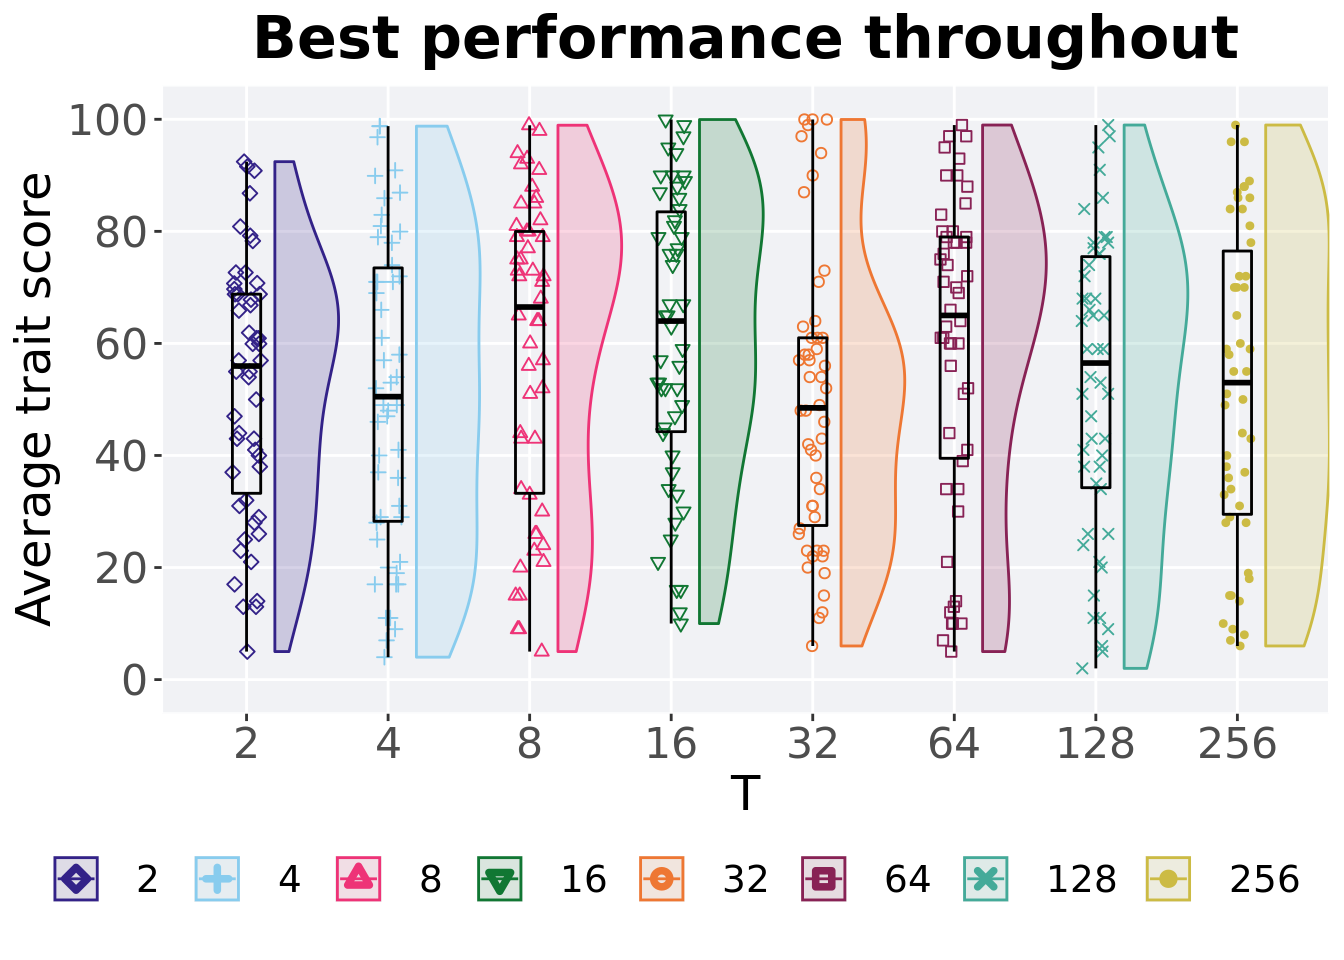
\includegraphics{demo_files/figure-latex/unnamed-chunk-131-1.pdf}

\hypertarget{stats-25}{%
\paragraph{Stats}\label{stats-25}}

Summary statistics for the performance of the best performing solution found throughout 50,000 generations.

\begin{Shaded}
\begin{Highlighting}[]
\KeywordTok{group_by}\NormalTok{(best, T) }\OperatorTok
\StringTok{  }\NormalTok{dplyr}\OperatorTok{::}\KeywordTok{summarise}\NormalTok{(}
    \DataTypeTok{count =} \KeywordTok{n}\NormalTok{(),}
    \DataTypeTok{na_cnt =} \KeywordTok{sum}\NormalTok{(}\KeywordTok{is.na}\NormalTok{(val)),}
    \DataTypeTok{min =} \KeywordTok{min}\NormalTok{(val }\OperatorTok{/}\StringTok{ }\NormalTok{TRAITS, }\DataTypeTok{na.rm =} \OtherTok{TRUE}\NormalTok{),}
    \DataTypeTok{median =} \KeywordTok{median}\NormalTok{(val }\OperatorTok{/}\StringTok{ }\NormalTok{TRAITS, }\DataTypeTok{na.rm =} \OtherTok{TRUE}\NormalTok{),}
    \DataTypeTok{mean =} \KeywordTok{mean}\NormalTok{(val }\OperatorTok{/}\StringTok{ }\NormalTok{TRAITS, }\DataTypeTok{na.rm =} \OtherTok{TRUE}\NormalTok{),}
    \DataTypeTok{max =} \KeywordTok{max}\NormalTok{(val }\OperatorTok{/}\StringTok{ }\NormalTok{TRAITS, }\DataTypeTok{na.rm =} \OtherTok{TRUE}\NormalTok{),}
    \DataTypeTok{IQR =} \KeywordTok{IQR}\NormalTok{(val }\OperatorTok{/}\StringTok{ }\NormalTok{TRAITS, }\DataTypeTok{na.rm =} \OtherTok{TRUE}\NormalTok{)}
\NormalTok{  )}
\end{Highlighting}
\end{Shaded}

\begin{verbatim}
## # A tibble: 8 x 8
##   T     count na_cnt   min median  mean   max   IQR
##   <fct> <int>  <int> <dbl>  <dbl> <dbl> <dbl> <dbl>
## 1 2        50      0  5      56.0  52.1  92.4  35.5
## 2 4        50      0  4      50.5  51.3  98.8  45.2
## 3 8        50      0  5      66.5  58.7  98.9  46.7
## 4 16       50      0 10.0    64.0  61.2 100.   39.2
## 5 32       50      0  6.00   48.5  49.9 100.   33.5
## 6 64       50      0  5      65.0  59.1  99.0  39.5
## 7 128      50      0  2      56.5  52.5  99.0  41.2
## 8 256      50      0  6      53.0  52.0  99.0  47.0
\end{verbatim}

Kruskal--Wallis test provides evidence of no statistical differences among the best performing solution found throughout 50,000 generations.

\begin{Shaded}
\begin{Highlighting}[]
\KeywordTok{kruskal.test}\NormalTok{(val }\OperatorTok{~}\StringTok{ }\NormalTok{T,}\DataTypeTok{data =}\NormalTok{ best)}
\end{Highlighting}
\end{Shaded}

\begin{verbatim}
## 
##  Kruskal-Wallis rank sum test
## 
## data:  val by T
## Kruskal-Wallis chi-squared = 9.9954, df = 7, p-value = 0.1888
\end{verbatim}

\hypertarget{end-of-50000-generations-11}{%
\subsubsection{End of 50,000 generations}\label{end-of-50000-generations-11}}

Best performance in the population at the end of 50,000 generations.

\begin{Shaded}
\begin{Highlighting}[]
\NormalTok{end =}\StringTok{ }\KeywordTok{filter}\NormalTok{(tor_end, diagnostic }\OperatorTok{==}\StringTok{ 'multipath_exploration'}\NormalTok{)}
\NormalTok{plot =}\StringTok{ }\KeywordTok{ggplot}\NormalTok{(end, }\KeywordTok{aes}\NormalTok{(}\DataTypeTok{x =}\NormalTok{ T, }\DataTypeTok{y =}\NormalTok{ pop_fit_max }\OperatorTok{/}\StringTok{ }\NormalTok{TRAITS, }\DataTypeTok{color =}\NormalTok{ T, }\DataTypeTok{fill =}\NormalTok{ T, }\DataTypeTok{shape =}\NormalTok{ T)) }\OperatorTok{+}
\StringTok{  }\KeywordTok{geom_flat_violin}\NormalTok{(}\DataTypeTok{position =} \KeywordTok{position_nudge}\NormalTok{(}\DataTypeTok{x =} \FloatTok{.2}\NormalTok{, }\DataTypeTok{y =} \DecValTok{0}\NormalTok{), }\DataTypeTok{scale =} \StringTok{'width'}\NormalTok{, }\DataTypeTok{alpha =} \FloatTok{0.2}\NormalTok{) }\OperatorTok{+}
\StringTok{  }\KeywordTok{geom_point}\NormalTok{(}\DataTypeTok{position =} \KeywordTok{position_jitter}\NormalTok{(}\DataTypeTok{width =} \FloatTok{.1}\NormalTok{), }\DataTypeTok{size =} \FloatTok{1.5}\NormalTok{, }\DataTypeTok{alpha =} \FloatTok{1.0}\NormalTok{) }\OperatorTok{+}
\StringTok{  }\KeywordTok{geom_boxplot}\NormalTok{(}\DataTypeTok{color =} \StringTok{'black'}\NormalTok{, }\DataTypeTok{width =} \FloatTok{.2}\NormalTok{, }\DataTypeTok{outlier.shape =} \OtherTok{NA}\NormalTok{, }\DataTypeTok{alpha =} \FloatTok{0.0}\NormalTok{) }\OperatorTok{+}
\StringTok{  }\KeywordTok{scale_y_continuous}\NormalTok{(}
    \DataTypeTok{name=}\StringTok{"Average trait score"}\NormalTok{,}
    \DataTypeTok{limits=}\KeywordTok{c}\NormalTok{(}\OperatorTok{-}\DecValTok{1}\NormalTok{, }\DecValTok{101}\NormalTok{),}
    \DataTypeTok{breaks=}\KeywordTok{seq}\NormalTok{(}\DecValTok{0}\NormalTok{,}\DecValTok{100}\NormalTok{, }\DecValTok{20}\NormalTok{),}
    \DataTypeTok{labels=}\KeywordTok{c}\NormalTok{(}\StringTok{"0"}\NormalTok{, }\StringTok{"20"}\NormalTok{, }\StringTok{"40"}\NormalTok{, }\StringTok{"60"}\NormalTok{, }\StringTok{"80"}\NormalTok{, }\StringTok{"100"}\NormalTok{)}
\NormalTok{  ) }\OperatorTok{+}
\StringTok{  }\KeywordTok{scale_x_discrete}\NormalTok{(}
    \DataTypeTok{name=}\StringTok{"T"}
\NormalTok{  )}\OperatorTok{+}
\StringTok{  }\KeywordTok{scale_shape_manual}\NormalTok{(}\DataTypeTok{values=}\NormalTok{SHAPE)}\OperatorTok{+}
\StringTok{  }\KeywordTok{scale_colour_manual}\NormalTok{(}\DataTypeTok{values =}\NormalTok{ cb_palette) }\OperatorTok{+}
\StringTok{  }\KeywordTok{scale_fill_manual}\NormalTok{(}\DataTypeTok{values =}\NormalTok{ cb_palette) }\OperatorTok{+}
\StringTok{  }\NormalTok{p_theme}

\KeywordTok{plot_grid}\NormalTok{(}
\NormalTok{  plot }\OperatorTok{+}
\StringTok{    }\KeywordTok{ggtitle}\NormalTok{(}\StringTok{"Final performance"}\NormalTok{) }\OperatorTok{+}
\StringTok{    }\KeywordTok{theme}\NormalTok{(}\DataTypeTok{legend.position=}\StringTok{"none"}\NormalTok{),}
\NormalTok{  legend,}
  \DataTypeTok{nrow=}\DecValTok{2}\NormalTok{,}
  \DataTypeTok{rel_heights =} \KeywordTok{c}\NormalTok{(}\DecValTok{2}\NormalTok{,.}\DecValTok{3}\NormalTok{),}
  \DataTypeTok{label_size =}\NormalTok{ TSIZE}
\NormalTok{)}
\end{Highlighting}
\end{Shaded}

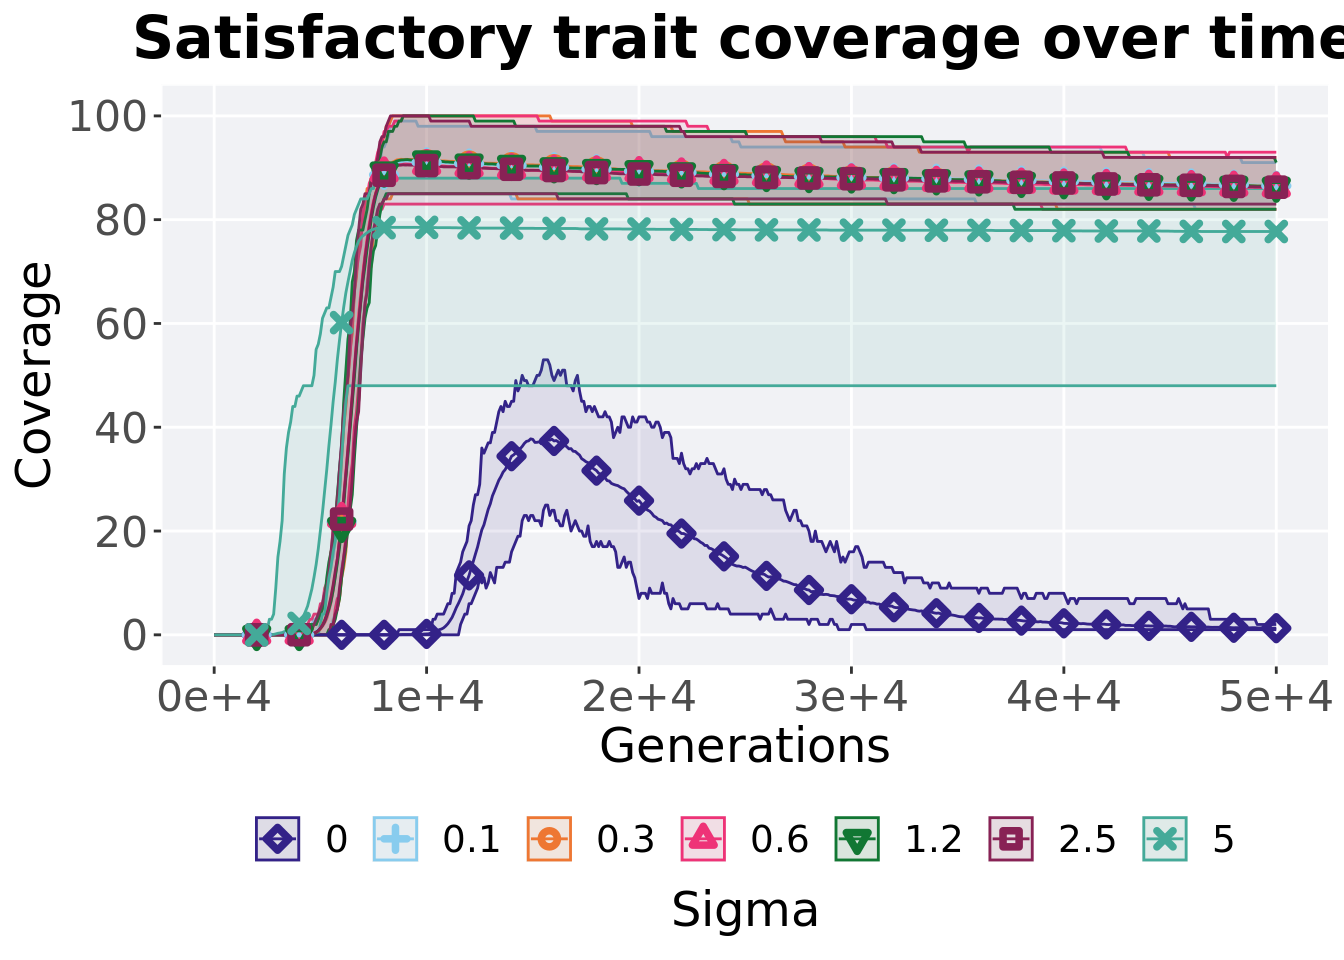
\includegraphics{demo_files/figure-latex/unnamed-chunk-134-1.pdf}

\hypertarget{stats-26}{%
\paragraph{Stats}\label{stats-26}}

Summary statistics for the best performance in the population at the end of 50,000 generations.

\begin{Shaded}
\begin{Highlighting}[]
\KeywordTok{group_by}\NormalTok{(end, T) }\OperatorTok
\StringTok{  }\NormalTok{dplyr}\OperatorTok{::}\KeywordTok{summarise}\NormalTok{(}
    \DataTypeTok{count =} \KeywordTok{n}\NormalTok{(),}
    \DataTypeTok{na_cnt =} \KeywordTok{sum}\NormalTok{(}\KeywordTok{is.na}\NormalTok{(pop_fit_max }\OperatorTok{/}\StringTok{ }\NormalTok{TRAITS)),}
    \DataTypeTok{min =} \KeywordTok{min}\NormalTok{(pop_fit_max }\OperatorTok{/}\StringTok{ }\NormalTok{TRAITS, }\DataTypeTok{na.rm =} \OtherTok{TRUE}\NormalTok{),}
    \DataTypeTok{median =} \KeywordTok{median}\NormalTok{(pop_fit_max }\OperatorTok{/}\StringTok{ }\NormalTok{TRAITS, }\DataTypeTok{na.rm =} \OtherTok{TRUE}\NormalTok{),}
    \DataTypeTok{mean =} \KeywordTok{mean}\NormalTok{(pop_fit_max }\OperatorTok{/}\StringTok{ }\NormalTok{TRAITS, }\DataTypeTok{na.rm =} \OtherTok{TRUE}\NormalTok{),}
    \DataTypeTok{max =} \KeywordTok{max}\NormalTok{(pop_fit_max }\OperatorTok{/}\StringTok{ }\NormalTok{TRAITS, }\DataTypeTok{na.rm =} \OtherTok{TRUE}\NormalTok{),}
    \DataTypeTok{IQR =} \KeywordTok{IQR}\NormalTok{(pop_fit_max }\OperatorTok{/}\StringTok{ }\NormalTok{TRAITS, }\DataTypeTok{na.rm =} \OtherTok{TRUE}\NormalTok{)}
\NormalTok{  )}
\end{Highlighting}
\end{Shaded}

\begin{verbatim}
## # A tibble: 8 x 8
##   T     count na_cnt   min median  mean   max   IQR
##   <fct> <int>  <int> <dbl>  <dbl> <dbl> <dbl> <dbl>
## 1 2        50      0  5      56.0  52.1  92.4  35.5
## 2 4        50      0  4      50.5  51.3  98.8  45.2
## 3 8        50      0  5      66.5  58.7  98.9  46.7
## 4 16       50      0 10.0    64.0  61.2 100.   39.2
## 5 32       50      0  6.00   48.5  49.9 100.   33.5
## 6 64       50      0  5      65.0  59.1  99.0  39.5
## 7 128      50      0  2      56.5  52.5  99.0  41.2
## 8 256      50      0  6      53.0  52.0  99.0  47.0
\end{verbatim}

Kruskal--Wallis test provides evidence of statistical differences among best performance in the population at the end of 50,000 generations.

\begin{Shaded}
\begin{Highlighting}[]
\KeywordTok{kruskal.test}\NormalTok{(pop_fit_max }\OperatorTok{~}\StringTok{ }\NormalTok{T, }\DataTypeTok{data =}\NormalTok{ end)}
\end{Highlighting}
\end{Shaded}

\begin{verbatim}
## 
##  Kruskal-Wallis rank sum test
## 
## data:  pop_fit_max by T
## Kruskal-Wallis chi-squared = 9.9954, df = 7, p-value = 0.1888
\end{verbatim}

Results for post-hoc Wilcoxon rank-sum test with a Bonferroni correction on the best performance in the population at the end of 50,000 generations.

\begin{Shaded}
\begin{Highlighting}[]
\KeywordTok{pairwise.wilcox.test}\NormalTok{(}\DataTypeTok{x =}\NormalTok{ end}\OperatorTok{$}\NormalTok{pop_fit_max, }\DataTypeTok{g =}\NormalTok{ end}\OperatorTok{$}\NormalTok{T , }\DataTypeTok{p.adjust.method =} \StringTok{"bonferroni"}\NormalTok{,}
                     \DataTypeTok{paired =} \OtherTok{FALSE}\NormalTok{, }\DataTypeTok{conf.int =} \OtherTok{FALSE}\NormalTok{, }\DataTypeTok{alternative =} \StringTok{'l'}\NormalTok{)}
\end{Highlighting}
\end{Shaded}

\begin{verbatim}
## 
##  Pairwise comparisons using Wilcoxon rank sum test with continuity correction 
## 
## data:  end$pop_fit_max and end$T 
## 
##     2    4    8    16   32   64   128 
## 4   1.00 -    -    -    -    -    -   
## 8   1.00 1.00 -    -    -    -    -   
## 16  1.00 1.00 1.00 -    -    -    -   
## 32  1.00 1.00 1.00 0.59 -    -    -   
## 64  1.00 1.00 1.00 1.00 1.00 -    -   
## 128 1.00 1.00 1.00 1.00 1.00 1.00 -   
## 256 1.00 1.00 1.00 1.00 1.00 1.00 1.00
## 
## P value adjustment method: bonferroni
\end{verbatim}

\hypertarget{activation-gene-coverage-5}{%
\subsection{Activation gene coverage}\label{activation-gene-coverage-5}}

Here we analyze the activation gene coverage for each parameter replicate on the multi-path exploration diagnostic.

\hypertarget{coverage-over-time-7}{%
\subsubsection{Coverage over time}\label{coverage-over-time-7}}

Activation gene coverage over time.

\begin{Shaded}
\begin{Highlighting}[]
\NormalTok{problem <-}\StringTok{ }\KeywordTok{filter}\NormalTok{(tor_ot, diagnostic }\OperatorTok{==}\StringTok{ 'multipath_exploration'}\NormalTok{)}
\NormalTok{lines =}\StringTok{ }\NormalTok{problem }\OperatorTok
\StringTok{        }\KeywordTok{group_by}\NormalTok{(T, gen) }\OperatorTok
\StringTok{          }\NormalTok{dplyr}\OperatorTok{::}\KeywordTok{summarise}\NormalTok{(}
            \DataTypeTok{min =} \KeywordTok{min}\NormalTok{(uni_str_pos),}
            \DataTypeTok{mean =} \KeywordTok{mean}\NormalTok{(uni_str_pos),}
            \DataTypeTok{max =} \KeywordTok{max}\NormalTok{(uni_str_pos)}
\NormalTok{          )}
\end{Highlighting}
\end{Shaded}

\begin{verbatim}
## `summarise()` has grouped output by 'T'. You can override using the `.groups`
## argument.
\end{verbatim}

\begin{Shaded}
\begin{Highlighting}[]
\NormalTok{points =}\StringTok{ }\KeywordTok{filter}\NormalTok{(lines, gen }\OperatorTok\StringTok{ }\DecValTok{2000} \OperatorTok{==}\StringTok{ }\DecValTok{0} \OperatorTok{&}\StringTok{ }\NormalTok{gen }\OperatorTok{!=}\StringTok{ }\DecValTok{0}\NormalTok{)}

\NormalTok{ot =}\StringTok{ }\KeywordTok{ggplot}\NormalTok{(lines, }\KeywordTok{aes}\NormalTok{(}\DataTypeTok{x=}\NormalTok{gen, }\DataTypeTok{y=}\NormalTok{mean, }\DataTypeTok{group =}\NormalTok{ T, }\DataTypeTok{fill =}\NormalTok{T, }\DataTypeTok{color =}\NormalTok{ T, }\DataTypeTok{shape =}\NormalTok{ T)) }\OperatorTok{+}
\StringTok{  }\KeywordTok{geom_ribbon}\NormalTok{(}\KeywordTok{aes}\NormalTok{(}\DataTypeTok{ymin =}\NormalTok{ min, }\DataTypeTok{ymax =}\NormalTok{ max), }\DataTypeTok{alpha =} \FloatTok{0.1}\NormalTok{) }\OperatorTok{+}
\StringTok{  }\KeywordTok{geom_line}\NormalTok{(}\DataTypeTok{size =} \FloatTok{0.5}\NormalTok{) }\OperatorTok{+}
\StringTok{  }\KeywordTok{geom_point}\NormalTok{(}\DataTypeTok{data =}\NormalTok{ points, }\DataTypeTok{size =} \FloatTok{1.5}\NormalTok{, }\DataTypeTok{stroke =} \FloatTok{2.0}\NormalTok{, }\DataTypeTok{alpha =} \FloatTok{1.0}\NormalTok{) }\OperatorTok{+}
\StringTok{  }\KeywordTok{scale_y_continuous}\NormalTok{(}
    \DataTypeTok{name=}\StringTok{"Coverage"}\NormalTok{,}
    \DataTypeTok{limits=}\KeywordTok{c}\NormalTok{(}\OperatorTok{-}\DecValTok{1}\NormalTok{, }\DecValTok{101}\NormalTok{),}
    \DataTypeTok{breaks=}\KeywordTok{seq}\NormalTok{(}\DecValTok{0}\NormalTok{,}\DecValTok{100}\NormalTok{, }\DecValTok{20}\NormalTok{),}
    \DataTypeTok{labels=}\KeywordTok{c}\NormalTok{(}\StringTok{"0"}\NormalTok{, }\StringTok{"20"}\NormalTok{, }\StringTok{"40"}\NormalTok{, }\StringTok{"60"}\NormalTok{, }\StringTok{"80"}\NormalTok{, }\StringTok{"100"}\NormalTok{)}
\NormalTok{  ) }\OperatorTok{+}
\StringTok{  }\KeywordTok{scale_x_continuous}\NormalTok{(}
    \DataTypeTok{name=}\StringTok{"Generations"}\NormalTok{,}
    \DataTypeTok{limits=}\KeywordTok{c}\NormalTok{(}\DecValTok{0}\NormalTok{, }\DecValTok{50000}\NormalTok{),}
    \DataTypeTok{breaks=}\KeywordTok{c}\NormalTok{(}\DecValTok{0}\NormalTok{, }\DecValTok{10000}\NormalTok{, }\DecValTok{20000}\NormalTok{, }\DecValTok{30000}\NormalTok{, }\DecValTok{40000}\NormalTok{, }\DecValTok{50000}\NormalTok{),}
    \DataTypeTok{labels=}\KeywordTok{c}\NormalTok{(}\StringTok{"0e+6"}\NormalTok{, }\StringTok{"1e+6"}\NormalTok{, }\StringTok{"2e+6"}\NormalTok{, }\StringTok{"3e+6"}\NormalTok{, }\StringTok{"4e+6"}\NormalTok{, }\StringTok{"5e+6"}\NormalTok{)}

\NormalTok{  ) }\OperatorTok{+}
\StringTok{  }\KeywordTok{scale_shape_manual}\NormalTok{(}\DataTypeTok{values=}\NormalTok{SHAPE)}\OperatorTok{+}
\StringTok{  }\KeywordTok{scale_colour_manual}\NormalTok{(}\DataTypeTok{values =}\NormalTok{ cb_palette) }\OperatorTok{+}
\StringTok{  }\KeywordTok{scale_fill_manual}\NormalTok{(}\DataTypeTok{values =}\NormalTok{ cb_palette) }\OperatorTok{+}
\StringTok{  }\KeywordTok{ggtitle}\NormalTok{(}\StringTok{"Activation gene coverage over time"}\NormalTok{) }\OperatorTok{+}
\StringTok{  }\NormalTok{p_theme}\OperatorTok{+}
\StringTok{    }\KeywordTok{guides}\NormalTok{(}
    \DataTypeTok{shape=}\KeywordTok{guide_legend}\NormalTok{(}\DataTypeTok{nrow=}\DecValTok{1}\NormalTok{, }\DataTypeTok{title.position =} \StringTok{"bottom"}\NormalTok{),}
    \DataTypeTok{color=}\KeywordTok{guide_legend}\NormalTok{(}\DataTypeTok{nrow=}\DecValTok{1}\NormalTok{, }\DataTypeTok{title.position =} \StringTok{"bottom"}\NormalTok{),}
    \DataTypeTok{fill=}\KeywordTok{guide_legend}\NormalTok{(}\DataTypeTok{nrow=}\DecValTok{1}\NormalTok{, }\DataTypeTok{title.position =} \StringTok{"bottom"}\NormalTok{)}
\NormalTok{  ) }\OperatorTok{+}
\StringTok{  }\KeywordTok{theme}\NormalTok{(}
    \DataTypeTok{legend.position =} \StringTok{"bottom"}\NormalTok{,}
    \DataTypeTok{legend.box=}\StringTok{"verticle"}\NormalTok{,}
    \DataTypeTok{legend.justification=}\StringTok{"center"}\NormalTok{,}
    \DataTypeTok{legend.title.align=}\FloatTok{0.5}
\NormalTok{  )}

\NormalTok{ot}
\end{Highlighting}
\end{Shaded}

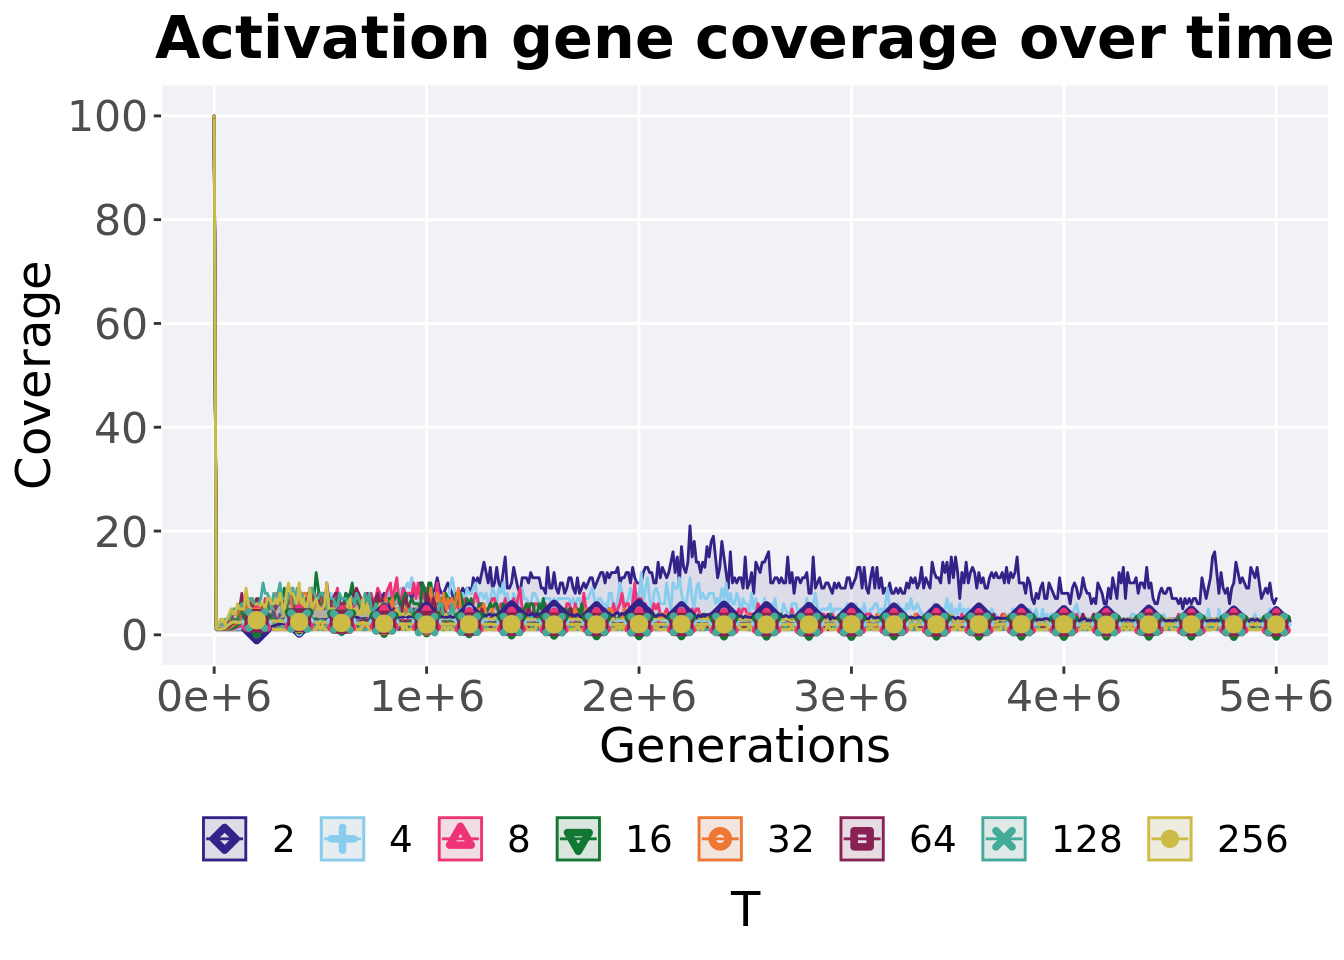
\includegraphics{demo_files/figure-latex/unnamed-chunk-138-1.pdf}

\hypertarget{end-of-50000-generations-12}{%
\subsubsection{End of 50,000 generations}\label{end-of-50000-generations-12}}

Activation gene coverage in the population at the end of 50,000 generations.

\begin{Shaded}
\begin{Highlighting}[]
\NormalTok{end =}\StringTok{ }\KeywordTok{filter}\NormalTok{(tor_end, diagnostic }\OperatorTok{==}\StringTok{ 'multipath_exploration'}\NormalTok{)}
\NormalTok{plot =}\StringTok{ }\KeywordTok{ggplot}\NormalTok{(end, }\KeywordTok{aes}\NormalTok{(}\DataTypeTok{x =}\NormalTok{ T, }\DataTypeTok{y =}\NormalTok{ uni_str_pos, }\DataTypeTok{color =}\NormalTok{ T, }\DataTypeTok{fill =}\NormalTok{ T, }\DataTypeTok{shape =}\NormalTok{ T)) }\OperatorTok{+}
\StringTok{  }\KeywordTok{geom_flat_violin}\NormalTok{(}\DataTypeTok{position =} \KeywordTok{position_nudge}\NormalTok{(}\DataTypeTok{x =} \FloatTok{.2}\NormalTok{, }\DataTypeTok{y =} \DecValTok{0}\NormalTok{), }\DataTypeTok{scale =} \StringTok{'width'}\NormalTok{, }\DataTypeTok{alpha =} \FloatTok{0.2}\NormalTok{) }\OperatorTok{+}
\StringTok{  }\KeywordTok{geom_point}\NormalTok{(}\DataTypeTok{position =} \KeywordTok{position_jitter}\NormalTok{(}\DataTypeTok{width =} \FloatTok{.1}\NormalTok{), }\DataTypeTok{size =} \FloatTok{1.5}\NormalTok{, }\DataTypeTok{alpha =} \FloatTok{1.0}\NormalTok{) }\OperatorTok{+}
\StringTok{  }\KeywordTok{geom_boxplot}\NormalTok{(}\DataTypeTok{color =} \StringTok{'black'}\NormalTok{, }\DataTypeTok{width =} \FloatTok{.2}\NormalTok{, }\DataTypeTok{outlier.shape =} \OtherTok{NA}\NormalTok{, }\DataTypeTok{alpha =} \FloatTok{0.0}\NormalTok{) }\OperatorTok{+}
\StringTok{  }\KeywordTok{scale_y_continuous}\NormalTok{(}
    \DataTypeTok{name=}\StringTok{"Coverage"}\NormalTok{,}
    \DataTypeTok{limits=}\KeywordTok{c}\NormalTok{(}\OperatorTok{-}\DecValTok{1}\NormalTok{, }\DecValTok{10}\NormalTok{),}
    \DataTypeTok{breaks=}\KeywordTok{seq}\NormalTok{(}\DecValTok{0}\NormalTok{,}\DecValTok{10}\NormalTok{, }\DecValTok{2}\NormalTok{),}
    \DataTypeTok{labels=}\KeywordTok{c}\NormalTok{(}\StringTok{"0"}\NormalTok{, }\StringTok{"2"}\NormalTok{, }\StringTok{"4"}\NormalTok{, }\StringTok{"6"}\NormalTok{, }\StringTok{"8"}\NormalTok{, }\StringTok{"10"}\NormalTok{)}
\NormalTok{  ) }\OperatorTok{+}
\StringTok{  }\KeywordTok{scale_x_discrete}\NormalTok{(}
    \DataTypeTok{name=}\StringTok{"T"}
\NormalTok{  )}\OperatorTok{+}
\StringTok{  }\KeywordTok{scale_shape_manual}\NormalTok{(}\DataTypeTok{values=}\NormalTok{SHAPE)}\OperatorTok{+}
\StringTok{  }\KeywordTok{scale_colour_manual}\NormalTok{(}\DataTypeTok{values =}\NormalTok{ cb_palette) }\OperatorTok{+}
\StringTok{  }\KeywordTok{scale_fill_manual}\NormalTok{(}\DataTypeTok{values =}\NormalTok{ cb_palette) }\OperatorTok{+}
\StringTok{  }\NormalTok{p_theme}

\KeywordTok{plot_grid}\NormalTok{(}
\NormalTok{  plot }\OperatorTok{+}
\StringTok{    }\KeywordTok{ggtitle}\NormalTok{(}\StringTok{"Final activation gene coverage"}\NormalTok{) }\OperatorTok{+}
\StringTok{    }\KeywordTok{theme}\NormalTok{(}\DataTypeTok{legend.position=}\StringTok{"none"}\NormalTok{),}
\NormalTok{  legend,}
  \DataTypeTok{nrow=}\DecValTok{2}\NormalTok{,}
  \DataTypeTok{rel_heights =} \KeywordTok{c}\NormalTok{(}\DecValTok{2}\NormalTok{,.}\DecValTok{3}\NormalTok{),}
  \DataTypeTok{label_size =}\NormalTok{ TSIZE}
\NormalTok{)}
\end{Highlighting}
\end{Shaded}

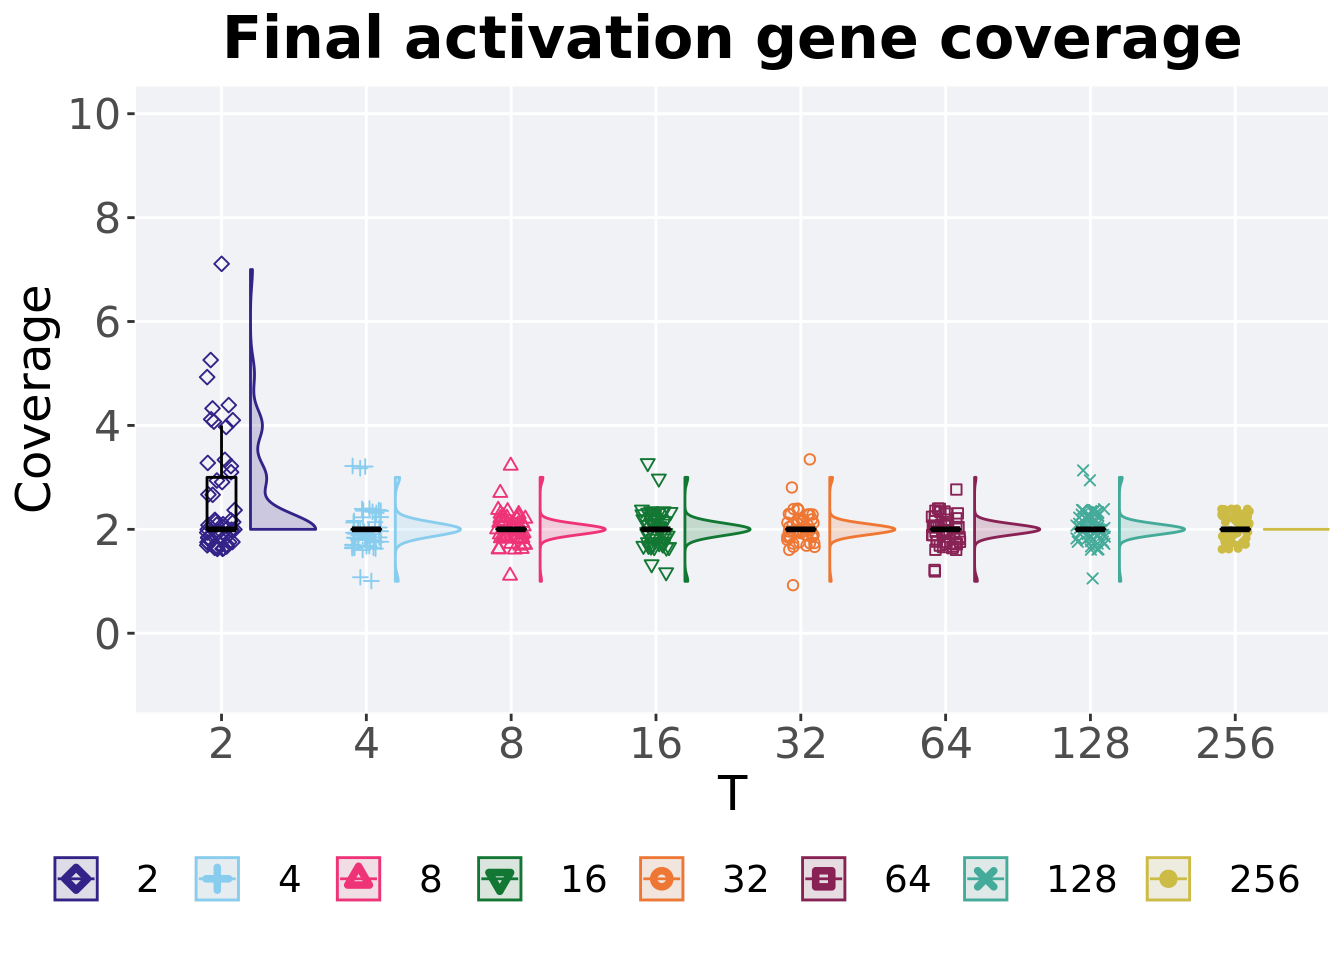
\includegraphics{demo_files/figure-latex/unnamed-chunk-139-1.pdf}

\hypertarget{stats-27}{%
\paragraph{Stats}\label{stats-27}}

Summary statistics for the activation gene coverage in the population at the end of 50,000 generations.

\begin{Shaded}
\begin{Highlighting}[]
\KeywordTok{group_by}\NormalTok{(end, T) }\OperatorTok
\StringTok{  }\NormalTok{dplyr}\OperatorTok{::}\KeywordTok{summarise}\NormalTok{(}
    \DataTypeTok{count =} \KeywordTok{n}\NormalTok{(),}
    \DataTypeTok{na_cnt =} \KeywordTok{sum}\NormalTok{(}\KeywordTok{is.na}\NormalTok{(uni_str_pos)),}
    \DataTypeTok{min =} \KeywordTok{min}\NormalTok{(uni_str_pos, }\DataTypeTok{na.rm =} \OtherTok{TRUE}\NormalTok{),}
    \DataTypeTok{median =} \KeywordTok{median}\NormalTok{(uni_str_pos, }\DataTypeTok{na.rm =} \OtherTok{TRUE}\NormalTok{),}
    \DataTypeTok{mean =} \KeywordTok{mean}\NormalTok{(uni_str_pos, }\DataTypeTok{na.rm =} \OtherTok{TRUE}\NormalTok{),}
    \DataTypeTok{max =} \KeywordTok{max}\NormalTok{(uni_str_pos, }\DataTypeTok{na.rm =} \OtherTok{TRUE}\NormalTok{),}
    \DataTypeTok{IQR =} \KeywordTok{IQR}\NormalTok{(uni_str_pos, }\DataTypeTok{na.rm =} \OtherTok{TRUE}\NormalTok{)}
\NormalTok{  )}
\end{Highlighting}
\end{Shaded}

\begin{verbatim}
## # A tibble: 8 x 8
##   T     count na_cnt   min median  mean   max   IQR
##   <fct> <int>  <int> <int>  <dbl> <dbl> <int> <dbl>
## 1 2        50      0     2      2  2.62     7     1
## 2 4        50      0     1      2  2.02     3     0
## 3 8        50      0     1      2  2.02     3     0
## 4 16       50      0     1      2  2        3     0
## 5 32       50      0     1      2  2.02     3     0
## 6 64       50      0     1      2  1.98     3     0
## 7 128      50      0     1      2  2.02     3     0
## 8 256      50      0     2      2  2        2     0
\end{verbatim}

Kruskal--Wallis test provides evidence of statistical differences among activation gene coverage in the population at the end of 50,000 generations.

\begin{Shaded}
\begin{Highlighting}[]
\KeywordTok{kruskal.test}\NormalTok{(uni_str_pos }\OperatorTok{~}\StringTok{ }\NormalTok{T, }\DataTypeTok{data =}\NormalTok{ end)}
\end{Highlighting}
\end{Shaded}

\begin{verbatim}
## 
##  Kruskal-Wallis rank sum test
## 
## data:  uni_str_pos by T
## Kruskal-Wallis chi-squared = 55.517, df = 7, p-value = 1.178e-09
\end{verbatim}

Results for post-hoc Wilcoxon rank-sum test with a Bonferroni correction on the activation gene coverage in the population at the end of 50,000 generations.

\begin{Shaded}
\begin{Highlighting}[]
\KeywordTok{pairwise.wilcox.test}\NormalTok{(}\DataTypeTok{x =}\NormalTok{ end}\OperatorTok{$}\NormalTok{uni_str_pos, }\DataTypeTok{g =}\NormalTok{ end}\OperatorTok{$}\NormalTok{T , }\DataTypeTok{p.adjust.method =} \StringTok{"bonferroni"}\NormalTok{,}
                     \DataTypeTok{paired =} \OtherTok{FALSE}\NormalTok{, }\DataTypeTok{conf.int =} \OtherTok{FALSE}\NormalTok{, }\DataTypeTok{alternative =} \StringTok{'t'}\NormalTok{)}
\end{Highlighting}
\end{Shaded}

\begin{verbatim}
## 
##  Pairwise comparisons using Wilcoxon rank sum test with continuity correction 
## 
## data:  end$uni_str_pos and end$T 
## 
##     2       4       8       16      32      64      128    
## 4   0.00454 -       -       -       -       -       -      
## 8   0.00217 1.00000 -       -       -       -       -      
## 16  0.00151 1.00000 1.00000 -       -       -       -      
## 32  0.00217 1.00000 1.00000 1.00000 -       -       -      
## 64  0.00044 1.00000 1.00000 1.00000 1.00000 -       -      
## 128 0.00217 1.00000 1.00000 1.00000 1.00000 1.00000 -      
## 256 0.00021 1.00000 1.00000 1.00000 1.00000 1.00000 1.00000
## 
## P value adjustment method: bonferroni
\end{verbatim}

\hypertarget{genotypic-fitness-sharing}{%
\chapter{Genotypic fitness sharing}\label{genotypic-fitness-sharing}}

We present the results from our parameter sweeep on genotypic fitness sharing.
50 replicates are conducted for each sigma parameter value explored.
Note that when \texttt{sigma\ =\ 0.0}, performance with no similarity penalty and stochastic remainder selection is used to identify parent solutions.

\begin{Shaded}
\begin{Highlighting}[]
\KeywordTok{library}\NormalTok{(ggplot2)}
\KeywordTok{library}\NormalTok{(cowplot)}
\KeywordTok{library}\NormalTok{(dplyr)}
\KeywordTok{library}\NormalTok{(PupillometryR)}
\end{Highlighting}
\end{Shaded}

These analyses were conducted in the following computing environment:

\begin{Shaded}
\begin{Highlighting}[]
\KeywordTok{print}\NormalTok{(version)}
\end{Highlighting}
\end{Shaded}

\begin{verbatim}
##                _                           
## platform       x86_64-pc-linux-gnu         
## arch           x86_64                      
## os             linux-gnu                   
## system         x86_64, linux-gnu           
## status                                     
## major          4                           
## minor          2.1                         
## year           2022                        
## month          06                          
## day            23                          
## svn rev        82513                       
## language       R                           
## version.string R version 4.2.1 (2022-06-23)
## nickname       Funny-Looking Kid
\end{verbatim}

\hypertarget{exploitation-rate-results-3}{%
\section{Exploitation rate results}\label{exploitation-rate-results-3}}

Here we present the results for \textbf{best performances} found by each genotypic fitness sharing sigma value replicate on the exploitation rate diagnostic.
50 replicates are conducted for each sigma parameter value explored.
Note that when \texttt{sigma\ =\ 0.0}, performance with no similarity penalty and stochastic remainder selection is used to identify parent solutions.

\hypertarget{performance-over-time-8}{%
\subsection{Performance over time}\label{performance-over-time-8}}

Performance over time.

\begin{Shaded}
\begin{Highlighting}[]
\NormalTok{problem <-}\StringTok{ }\KeywordTok{filter}\NormalTok{(gfs_ot, diagnostic }\OperatorTok{==}\StringTok{ 'exploitation_rate'}\NormalTok{)}
\NormalTok{lines =}\StringTok{ }\NormalTok{problem }\OperatorTok
\StringTok{        }\KeywordTok{group_by}\NormalTok{(Sigma, gen) }\OperatorTok
\StringTok{          }\NormalTok{dplyr}\OperatorTok{::}\KeywordTok{summarise}\NormalTok{(}
            \DataTypeTok{min =} \KeywordTok{min}\NormalTok{(pop_fit_max),}
            \DataTypeTok{mean =} \KeywordTok{mean}\NormalTok{(pop_fit_max),}
            \DataTypeTok{max =} \KeywordTok{max}\NormalTok{(pop_fit_max)}
\NormalTok{          )}
\end{Highlighting}
\end{Shaded}

\begin{verbatim}
## `summarise()` has grouped output by 'Sigma'. You can override using the
## `.groups` argument.
\end{verbatim}

\begin{Shaded}
\begin{Highlighting}[]
\NormalTok{points =}\StringTok{ }\KeywordTok{filter}\NormalTok{(lines, gen }\OperatorTok\StringTok{ }\DecValTok{2000} \OperatorTok{==}\StringTok{ }\DecValTok{0} \OperatorTok{&}\StringTok{ }\NormalTok{gen }\OperatorTok{!=}\StringTok{ }\DecValTok{0}\NormalTok{)}

\NormalTok{ot =}\StringTok{ }\KeywordTok{ggplot}\NormalTok{(lines, }\KeywordTok{aes}\NormalTok{(}\DataTypeTok{x=}\NormalTok{gen, }\DataTypeTok{y=}\NormalTok{mean }\OperatorTok{/}\StringTok{ }\NormalTok{TRAITS, }\DataTypeTok{group =}\NormalTok{ Sigma, }\DataTypeTok{fill =}\NormalTok{ Sigma, }\DataTypeTok{color =}\NormalTok{ Sigma, }\DataTypeTok{shape =}\NormalTok{ Sigma)) }\OperatorTok{+}
\StringTok{  }\KeywordTok{geom_ribbon}\NormalTok{(}\KeywordTok{aes}\NormalTok{(}\DataTypeTok{ymin =}\NormalTok{ min }\OperatorTok{/}\StringTok{ }\NormalTok{TRAITS, }\DataTypeTok{ymax =}\NormalTok{ max }\OperatorTok{/}\StringTok{ }\NormalTok{TRAITS), }\DataTypeTok{alpha =} \FloatTok{0.1}\NormalTok{) }\OperatorTok{+}
\StringTok{  }\KeywordTok{geom_line}\NormalTok{(}\DataTypeTok{size =} \FloatTok{0.5}\NormalTok{) }\OperatorTok{+}
\StringTok{  }\KeywordTok{geom_point}\NormalTok{(}\DataTypeTok{data =}\NormalTok{ points, }\DataTypeTok{size =} \FloatTok{1.5}\NormalTok{, }\DataTypeTok{stroke =} \FloatTok{2.0}\NormalTok{, }\DataTypeTok{alpha =} \FloatTok{1.0}\NormalTok{) }\OperatorTok{+}
\StringTok{  }\KeywordTok{scale_y_continuous}\NormalTok{(}
    \DataTypeTok{name=}\StringTok{"Average trait score"}\NormalTok{,}
    \DataTypeTok{limits=}\KeywordTok{c}\NormalTok{(}\OperatorTok{-}\DecValTok{1}\NormalTok{, }\DecValTok{101}\NormalTok{),}
    \DataTypeTok{breaks=}\KeywordTok{seq}\NormalTok{(}\DecValTok{0}\NormalTok{,}\DecValTok{100}\NormalTok{, }\DecValTok{20}\NormalTok{),}
    \DataTypeTok{labels=}\KeywordTok{c}\NormalTok{(}\StringTok{"0"}\NormalTok{, }\StringTok{"20"}\NormalTok{, }\StringTok{"40"}\NormalTok{, }\StringTok{"60"}\NormalTok{, }\StringTok{"80"}\NormalTok{, }\StringTok{"100"}\NormalTok{)}
\NormalTok{  ) }\OperatorTok{+}
\StringTok{  }\KeywordTok{scale_x_continuous}\NormalTok{(}
    \DataTypeTok{name=}\StringTok{"Generations"}\NormalTok{,}
    \DataTypeTok{limits=}\KeywordTok{c}\NormalTok{(}\DecValTok{0}\NormalTok{, }\DecValTok{50000}\NormalTok{),}
    \DataTypeTok{breaks=}\KeywordTok{c}\NormalTok{(}\DecValTok{0}\NormalTok{, }\DecValTok{10000}\NormalTok{, }\DecValTok{20000}\NormalTok{, }\DecValTok{30000}\NormalTok{, }\DecValTok{40000}\NormalTok{, }\DecValTok{50000}\NormalTok{),}
    \DataTypeTok{labels=}\KeywordTok{c}\NormalTok{(}\StringTok{"0e+6"}\NormalTok{, }\StringTok{"1e+6"}\NormalTok{, }\StringTok{"2e+6"}\NormalTok{, }\StringTok{"3e+6"}\NormalTok{, }\StringTok{"4e+6"}\NormalTok{, }\StringTok{"5e+6"}\NormalTok{)}

\NormalTok{  ) }\OperatorTok{+}
\StringTok{  }\KeywordTok{scale_shape_manual}\NormalTok{(}\DataTypeTok{values=}\NormalTok{SHAPE)}\OperatorTok{+}
\StringTok{  }\KeywordTok{scale_colour_manual}\NormalTok{(}\DataTypeTok{values =}\NormalTok{ cb_palette) }\OperatorTok{+}
\StringTok{  }\KeywordTok{scale_fill_manual}\NormalTok{(}\DataTypeTok{values =}\NormalTok{ cb_palette) }\OperatorTok{+}
\StringTok{  }\KeywordTok{ggtitle}\NormalTok{(}\StringTok{"Best performance over time"}\NormalTok{) }\OperatorTok{+}
\StringTok{  }\NormalTok{p_theme}\OperatorTok{+}
\StringTok{    }\KeywordTok{guides}\NormalTok{(}
    \DataTypeTok{shape=}\KeywordTok{guide_legend}\NormalTok{(}\DataTypeTok{nrow=}\DecValTok{1}\NormalTok{, }\DataTypeTok{title.position =} \StringTok{"bottom"}\NormalTok{),}
    \DataTypeTok{color=}\KeywordTok{guide_legend}\NormalTok{(}\DataTypeTok{nrow=}\DecValTok{1}\NormalTok{, }\DataTypeTok{title.position =} \StringTok{"bottom"}\NormalTok{),}
    \DataTypeTok{fill=}\KeywordTok{guide_legend}\NormalTok{(}\DataTypeTok{nrow=}\DecValTok{1}\NormalTok{, }\DataTypeTok{title.position =} \StringTok{"bottom"}\NormalTok{)}
\NormalTok{  ) }\OperatorTok{+}
\StringTok{  }\KeywordTok{theme}\NormalTok{(}
    \DataTypeTok{legend.position =} \StringTok{"bottom"}\NormalTok{,}
    \DataTypeTok{legend.box=}\StringTok{"verticle"}\NormalTok{,}
    \DataTypeTok{legend.justification=}\StringTok{"center"}\NormalTok{,}
    \DataTypeTok{legend.title.align=}\FloatTok{0.5}
\NormalTok{  )}

\NormalTok{ot}
\end{Highlighting}
\end{Shaded}

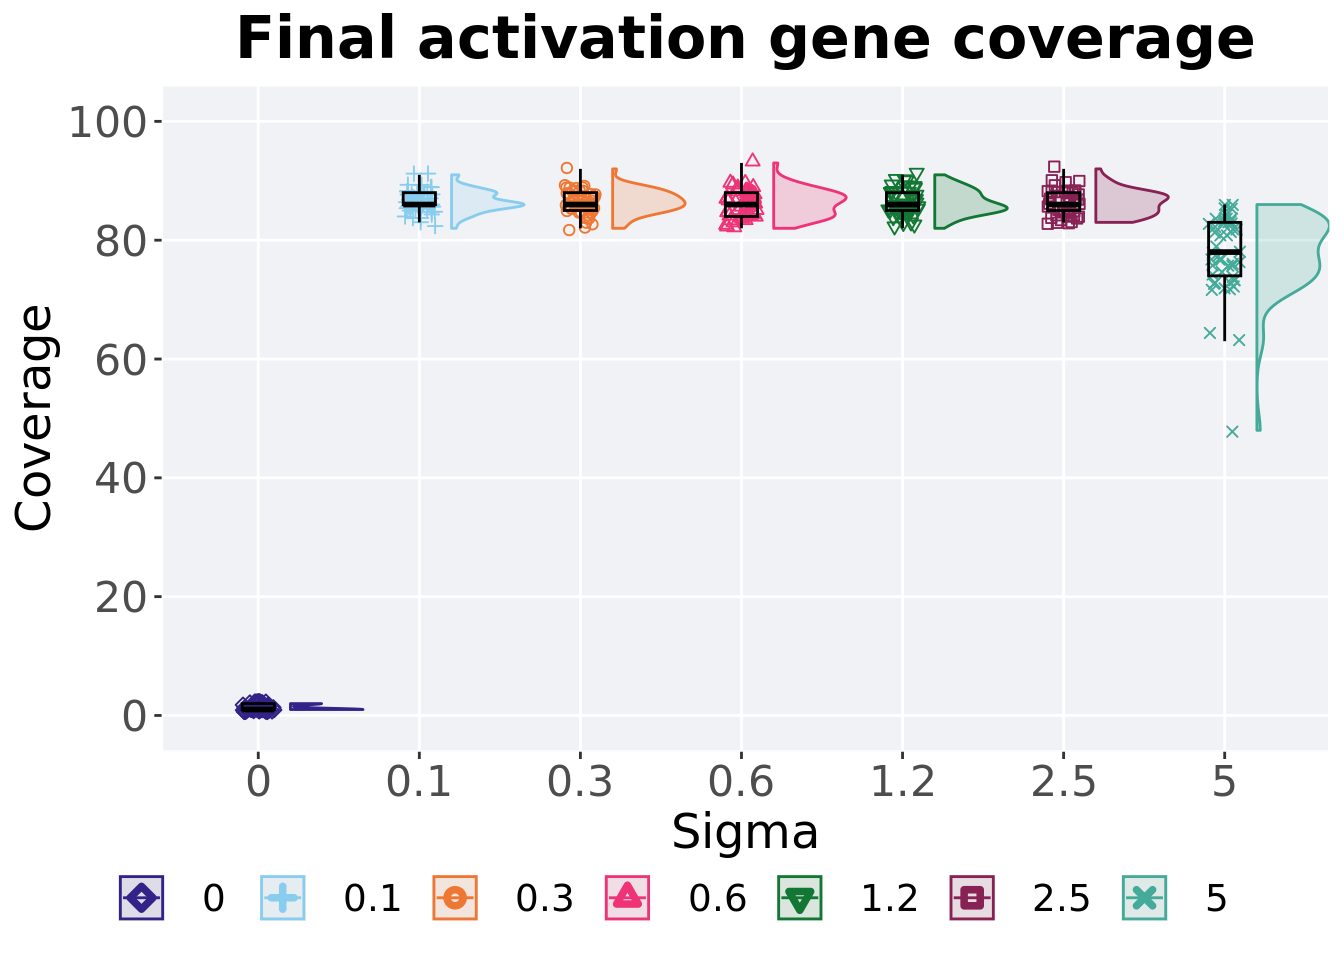
\includegraphics{demo_files/figure-latex/unnamed-chunk-145-1.pdf}

\hypertarget{best-performance-throughout-5}{%
\subsection{Best performance throughout}\label{best-performance-throughout-5}}

The best performance found throughout 50,000 generations.

\begin{Shaded}
\begin{Highlighting}[]
\NormalTok{best =}\StringTok{ }\KeywordTok{filter}\NormalTok{(gfs_best, col }\OperatorTok{==}\StringTok{ 'pop_fit_max'} \OperatorTok{&}\StringTok{ }\NormalTok{diagnostic }\OperatorTok{==}\StringTok{ 'exploitation_rate'}\NormalTok{)}

\NormalTok{plot =}\StringTok{ }\KeywordTok{ggplot}\NormalTok{(best, }\KeywordTok{aes}\NormalTok{(}\DataTypeTok{x =}\NormalTok{ Sigma, }\DataTypeTok{y =}\NormalTok{ val }\OperatorTok{/}\StringTok{ }\NormalTok{TRAITS, }\DataTypeTok{color =}\NormalTok{ Sigma, }\DataTypeTok{fill =}\NormalTok{ Sigma, }\DataTypeTok{shape =}\NormalTok{ Sigma)) }\OperatorTok{+}
\StringTok{  }\KeywordTok{geom_flat_violin}\NormalTok{(}\DataTypeTok{position =} \KeywordTok{position_nudge}\NormalTok{(}\DataTypeTok{x =} \FloatTok{.2}\NormalTok{, }\DataTypeTok{y =} \DecValTok{0}\NormalTok{), }\DataTypeTok{scale =} \StringTok{'width'}\NormalTok{, }\DataTypeTok{alpha =} \FloatTok{0.2}\NormalTok{) }\OperatorTok{+}
\StringTok{  }\KeywordTok{geom_point}\NormalTok{(}\DataTypeTok{position =} \KeywordTok{position_jitter}\NormalTok{(}\DataTypeTok{width =} \FloatTok{.1}\NormalTok{), }\DataTypeTok{size =} \FloatTok{1.5}\NormalTok{, }\DataTypeTok{alpha =} \FloatTok{1.0}\NormalTok{) }\OperatorTok{+}
\StringTok{  }\KeywordTok{geom_boxplot}\NormalTok{(}\DataTypeTok{color =} \StringTok{'black'}\NormalTok{, }\DataTypeTok{width =} \FloatTok{.2}\NormalTok{, }\DataTypeTok{outlier.shape =} \OtherTok{NA}\NormalTok{, }\DataTypeTok{alpha =} \FloatTok{0.0}\NormalTok{) }\OperatorTok{+}
\StringTok{  }\KeywordTok{scale_y_continuous}\NormalTok{(}
    \DataTypeTok{name=}\StringTok{"Average trait score"}\NormalTok{,}
    \DataTypeTok{limits=}\KeywordTok{c}\NormalTok{(}\OperatorTok{-}\DecValTok{1}\NormalTok{, }\DecValTok{101}\NormalTok{),}
    \DataTypeTok{breaks=}\KeywordTok{seq}\NormalTok{(}\DecValTok{0}\NormalTok{,}\DecValTok{100}\NormalTok{, }\DecValTok{20}\NormalTok{),}
    \DataTypeTok{labels=}\KeywordTok{c}\NormalTok{(}\StringTok{"0"}\NormalTok{, }\StringTok{"20"}\NormalTok{, }\StringTok{"40"}\NormalTok{, }\StringTok{"60"}\NormalTok{, }\StringTok{"80"}\NormalTok{, }\StringTok{"100"}\NormalTok{)}
\NormalTok{  ) }\OperatorTok{+}
\StringTok{  }\KeywordTok{scale_x_discrete}\NormalTok{(}
    \DataTypeTok{name=}\StringTok{"Sigma"}
\NormalTok{  )}\OperatorTok{+}
\StringTok{  }\KeywordTok{scale_shape_manual}\NormalTok{(}\DataTypeTok{values=}\NormalTok{SHAPE)}\OperatorTok{+}
\StringTok{  }\KeywordTok{scale_colour_manual}\NormalTok{(}\DataTypeTok{values =}\NormalTok{ cb_palette) }\OperatorTok{+}
\StringTok{  }\KeywordTok{scale_fill_manual}\NormalTok{(}\DataTypeTok{values =}\NormalTok{ cb_palette) }\OperatorTok{+}
\StringTok{  }\NormalTok{p_theme}

\KeywordTok{plot_grid}\NormalTok{(}
\NormalTok{  plot }\OperatorTok{+}
\StringTok{    }\KeywordTok{ggtitle}\NormalTok{(}\StringTok{"Best performance throughout"}\NormalTok{) }\OperatorTok{+}
\StringTok{    }\KeywordTok{theme}\NormalTok{(}\DataTypeTok{legend.position=}\StringTok{"none"}\NormalTok{),}
\NormalTok{  legend,}
  \DataTypeTok{nrow=}\DecValTok{2}\NormalTok{,}
  \DataTypeTok{rel_heights =} \KeywordTok{c}\NormalTok{(}\DecValTok{2}\NormalTok{,.}\DecValTok{3}\NormalTok{),}
  \DataTypeTok{label_size =}\NormalTok{ TSIZE}
\NormalTok{)}
\end{Highlighting}
\end{Shaded}

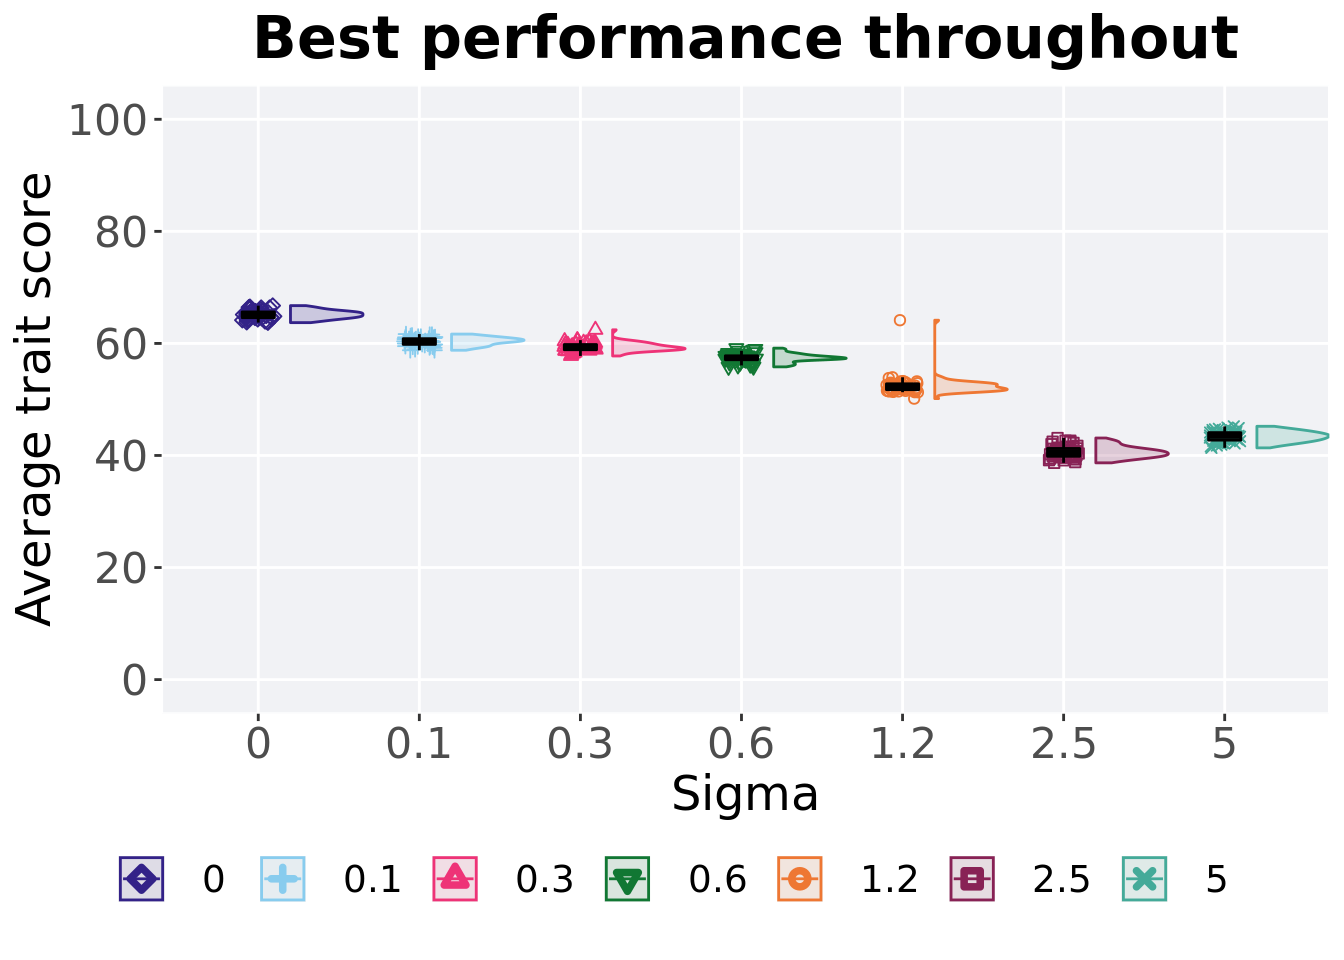
\includegraphics{demo_files/figure-latex/unnamed-chunk-147-1.pdf}

\hypertarget{stats-28}{%
\subsubsection{Stats}\label{stats-28}}

Summary statistics for the best performance found throughout 50,000 generations.

\begin{Shaded}
\begin{Highlighting}[]
\KeywordTok{group_by}\NormalTok{(best, Sigma) }\OperatorTok
\StringTok{  }\NormalTok{dplyr}\OperatorTok{::}\KeywordTok{summarise}\NormalTok{(}
    \DataTypeTok{count =} \KeywordTok{n}\NormalTok{(),}
    \DataTypeTok{na_cnt =} \KeywordTok{sum}\NormalTok{(}\KeywordTok{is.na}\NormalTok{(val)),}
    \DataTypeTok{min =} \KeywordTok{min}\NormalTok{(val }\OperatorTok{/}\StringTok{ }\NormalTok{TRAITS, }\DataTypeTok{na.rm =} \OtherTok{TRUE}\NormalTok{),}
    \DataTypeTok{median =} \KeywordTok{median}\NormalTok{(val }\OperatorTok{/}\StringTok{ }\NormalTok{TRAITS, }\DataTypeTok{na.rm =} \OtherTok{TRUE}\NormalTok{),}
    \DataTypeTok{mean =} \KeywordTok{mean}\NormalTok{(val }\OperatorTok{/}\StringTok{ }\NormalTok{TRAITS, }\DataTypeTok{na.rm =} \OtherTok{TRUE}\NormalTok{),}
    \DataTypeTok{max =} \KeywordTok{max}\NormalTok{(val }\OperatorTok{/}\StringTok{ }\NormalTok{TRAITS, }\DataTypeTok{na.rm =} \OtherTok{TRUE}\NormalTok{),}
    \DataTypeTok{IQR =} \KeywordTok{IQR}\NormalTok{(val }\OperatorTok{/}\StringTok{ }\NormalTok{TRAITS, }\DataTypeTok{na.rm =} \OtherTok{TRUE}\NormalTok{)}
\NormalTok{  )}
\end{Highlighting}
\end{Shaded}

\begin{verbatim}
## # A tibble: 7 x 8
##   Sigma count na_cnt   min median  mean   max   IQR
##   <fct> <int>  <int> <dbl>  <dbl> <dbl> <dbl> <dbl>
## 1 0        50      0  63.7   65.1  65.2  66.7 1.02 
## 2 0.1      50      0  58.8   60.4  60.4  61.7 1.02 
## 3 0.3      50      0  57.8   59.2  59.4  62.4 0.921
## 4 0.6      50      0  55.8   57.4  57.4  59.2 0.698
## 5 1.2      50      0  50.2   52.1  52.5  64.1 1.03 
## 6 2.5      50      0  38.7   40.5  40.6  43.1 1.38 
## 7 5        50      0  41.4   43.5  43.4  45.2 1.33
\end{verbatim}

Kruskal--Wallis test provides evidence of significant differences among sigma values on the best performance found throughout 50,000 generations

\begin{Shaded}
\begin{Highlighting}[]
\KeywordTok{kruskal.test}\NormalTok{(val }\OperatorTok{~}\StringTok{ }\NormalTok{Sigma,}\DataTypeTok{data =}\NormalTok{ best)}
\end{Highlighting}
\end{Shaded}

\begin{verbatim}
## 
##  Kruskal-Wallis rank sum test
## 
## data:  val by Sigma
## Kruskal-Wallis chi-squared = 333.76, df = 6, p-value < 2.2e-16
\end{verbatim}

Results for post-hoc Wilcoxon rank-sum test with a Bonferroni correction on the best performance found throughout 50,000 generations.

\begin{Shaded}
\begin{Highlighting}[]
\KeywordTok{pairwise.wilcox.test}\NormalTok{(}\DataTypeTok{x =}\NormalTok{ best}\OperatorTok{$}\NormalTok{val, }\DataTypeTok{g =}\NormalTok{ best}\OperatorTok{$}\NormalTok{Sigma , }\DataTypeTok{p.adjust.method =} \StringTok{"bonferroni"}\NormalTok{,}
                     \DataTypeTok{paired =} \OtherTok{FALSE}\NormalTok{, }\DataTypeTok{conf.int =} \OtherTok{FALSE}\NormalTok{, }\DataTypeTok{alternative =} \StringTok{'l'}\NormalTok{)}
\end{Highlighting}
\end{Shaded}

\begin{verbatim}
## 
##  Pairwise comparisons using Wilcoxon rank sum test with continuity correction 
## 
## data:  best$val and best$Sigma 
## 
##     0       0.1     0.3     0.6     1.2     2.5
## 0.1 < 2e-16 -       -       -       -       -  
## 0.3 < 2e-16 6.6e-08 -       -       -       -  
## 0.6 < 2e-16 < 2e-16 7.4e-15 -       -       -  
## 1.2 < 2e-16 1.4e-15 1.4e-15 1.4e-15 -       -  
## 2.5 < 2e-16 < 2e-16 < 2e-16 < 2e-16 < 2e-16 -  
## 5   < 2e-16 < 2e-16 < 2e-16 < 2e-16 < 2e-16 1  
## 
## P value adjustment method: bonferroni
\end{verbatim}

\hypertarget{ordered-exploitation-results-3}{%
\section{Ordered exploitation results}\label{ordered-exploitation-results-3}}

Here we present the results for \textbf{best performances} found by each genotypic fitness sharing sigma value replicate on the ordered exploitation diagnostic.
Best performance found refers to the largest average trait score found in a given population.
Note that performance values fall between 0 and 100.

\hypertarget{performance-over-time-9}{%
\subsection{Performance over time}\label{performance-over-time-9}}

Performance over time.

\begin{Shaded}
\begin{Highlighting}[]
\NormalTok{problem <-}\StringTok{ }\KeywordTok{filter}\NormalTok{(gfs_ot, diagnostic }\OperatorTok{==}\StringTok{ 'ordered_exploitation'}\NormalTok{)}
\NormalTok{lines =}\StringTok{ }\NormalTok{problem }\OperatorTok
\StringTok{        }\KeywordTok{group_by}\NormalTok{(Sigma, gen) }\OperatorTok
\StringTok{          }\NormalTok{dplyr}\OperatorTok{::}\KeywordTok{summarise}\NormalTok{(}
            \DataTypeTok{min =} \KeywordTok{min}\NormalTok{(pop_fit_max),}
            \DataTypeTok{mean =} \KeywordTok{mean}\NormalTok{(pop_fit_max),}
            \DataTypeTok{max =} \KeywordTok{max}\NormalTok{(pop_fit_max)}
\NormalTok{          )}
\end{Highlighting}
\end{Shaded}

\begin{verbatim}
## `summarise()` has grouped output by 'Sigma'. You can override using the
## `.groups` argument.
\end{verbatim}

\begin{Shaded}
\begin{Highlighting}[]
\NormalTok{points =}\StringTok{ }\KeywordTok{filter}\NormalTok{(lines, gen }\OperatorTok\StringTok{ }\DecValTok{2000} \OperatorTok{==}\StringTok{ }\DecValTok{0} \OperatorTok{&}\StringTok{ }\NormalTok{gen }\OperatorTok{!=}\StringTok{ }\DecValTok{0}\NormalTok{)}

\NormalTok{ot =}\StringTok{ }\KeywordTok{ggplot}\NormalTok{(lines, }\KeywordTok{aes}\NormalTok{(}\DataTypeTok{x=}\NormalTok{gen, }\DataTypeTok{y=}\NormalTok{mean }\OperatorTok{/}\StringTok{ }\NormalTok{TRAITS, }\DataTypeTok{group =}\NormalTok{ Sigma, }\DataTypeTok{fill =}\NormalTok{ Sigma, }\DataTypeTok{color =}\NormalTok{ Sigma, }\DataTypeTok{shape =}\NormalTok{ Sigma)) }\OperatorTok{+}
\StringTok{  }\KeywordTok{geom_ribbon}\NormalTok{(}\KeywordTok{aes}\NormalTok{(}\DataTypeTok{ymin =}\NormalTok{ min }\OperatorTok{/}\StringTok{ }\NormalTok{TRAITS, }\DataTypeTok{ymax =}\NormalTok{ max }\OperatorTok{/}\StringTok{ }\NormalTok{TRAITS), }\DataTypeTok{alpha =} \FloatTok{0.1}\NormalTok{) }\OperatorTok{+}
\StringTok{  }\KeywordTok{geom_line}\NormalTok{(}\DataTypeTok{size =} \FloatTok{0.5}\NormalTok{) }\OperatorTok{+}
\StringTok{  }\KeywordTok{geom_point}\NormalTok{(}\DataTypeTok{data =}\NormalTok{ points, }\DataTypeTok{size =} \FloatTok{1.5}\NormalTok{, }\DataTypeTok{stroke =} \FloatTok{2.0}\NormalTok{, }\DataTypeTok{alpha =} \FloatTok{1.0}\NormalTok{) }\OperatorTok{+}
\StringTok{  }\KeywordTok{scale_y_continuous}\NormalTok{(}
    \DataTypeTok{name=}\StringTok{"Average trait score"}\NormalTok{,}
    \DataTypeTok{limits=}\KeywordTok{c}\NormalTok{(}\OperatorTok{-}\DecValTok{1}\NormalTok{, }\DecValTok{30}\NormalTok{),}
    \DataTypeTok{breaks=}\KeywordTok{seq}\NormalTok{(}\DecValTok{0}\NormalTok{, }\DecValTok{30}\NormalTok{, }\DecValTok{10}\NormalTok{),}
    \DataTypeTok{labels=}\KeywordTok{c}\NormalTok{(}\StringTok{"0"}\NormalTok{, }\StringTok{"10"}\NormalTok{, }\StringTok{"20"}\NormalTok{, }\StringTok{"30"}\NormalTok{)}
\NormalTok{  ) }\OperatorTok{+}
\StringTok{  }\KeywordTok{scale_x_continuous}\NormalTok{(}
    \DataTypeTok{name=}\StringTok{"Generations"}\NormalTok{,}
    \DataTypeTok{limits=}\KeywordTok{c}\NormalTok{(}\DecValTok{0}\NormalTok{, }\DecValTok{50000}\NormalTok{),}
    \DataTypeTok{breaks=}\KeywordTok{c}\NormalTok{(}\DecValTok{0}\NormalTok{, }\DecValTok{10000}\NormalTok{, }\DecValTok{20000}\NormalTok{, }\DecValTok{30000}\NormalTok{, }\DecValTok{40000}\NormalTok{, }\DecValTok{50000}\NormalTok{),}
    \DataTypeTok{labels=}\KeywordTok{c}\NormalTok{(}\StringTok{"0e+6"}\NormalTok{, }\StringTok{"1e+6"}\NormalTok{, }\StringTok{"2e+6"}\NormalTok{, }\StringTok{"3e+6"}\NormalTok{, }\StringTok{"4e+6"}\NormalTok{, }\StringTok{"5e+6"}\NormalTok{)}

\NormalTok{  ) }\OperatorTok{+}
\StringTok{  }\KeywordTok{scale_shape_manual}\NormalTok{(}\DataTypeTok{values=}\NormalTok{SHAPE)}\OperatorTok{+}
\StringTok{  }\KeywordTok{scale_colour_manual}\NormalTok{(}\DataTypeTok{values =}\NormalTok{ cb_palette) }\OperatorTok{+}
\StringTok{  }\KeywordTok{scale_fill_manual}\NormalTok{(}\DataTypeTok{values =}\NormalTok{ cb_palette) }\OperatorTok{+}
\StringTok{  }\KeywordTok{ggtitle}\NormalTok{(}\StringTok{"Best performance over time"}\NormalTok{) }\OperatorTok{+}
\StringTok{  }\NormalTok{p_theme}\OperatorTok{+}
\StringTok{    }\KeywordTok{guides}\NormalTok{(}
    \DataTypeTok{shape=}\KeywordTok{guide_legend}\NormalTok{(}\DataTypeTok{nrow=}\DecValTok{1}\NormalTok{, }\DataTypeTok{title.position =} \StringTok{"bottom"}\NormalTok{),}
    \DataTypeTok{color=}\KeywordTok{guide_legend}\NormalTok{(}\DataTypeTok{nrow=}\DecValTok{1}\NormalTok{, }\DataTypeTok{title.position =} \StringTok{"bottom"}\NormalTok{),}
    \DataTypeTok{fill=}\KeywordTok{guide_legend}\NormalTok{(}\DataTypeTok{nrow=}\DecValTok{1}\NormalTok{, }\DataTypeTok{title.position =} \StringTok{"bottom"}\NormalTok{)}
\NormalTok{  ) }\OperatorTok{+}
\StringTok{  }\KeywordTok{theme}\NormalTok{(}
    \DataTypeTok{legend.position =} \StringTok{"bottom"}\NormalTok{,}
    \DataTypeTok{legend.box=}\StringTok{"verticle"}\NormalTok{,}
    \DataTypeTok{legend.justification=}\StringTok{"center"}\NormalTok{,}
    \DataTypeTok{legend.title.align=}\FloatTok{0.5}
\NormalTok{  )}

\NormalTok{ot}
\end{Highlighting}
\end{Shaded}

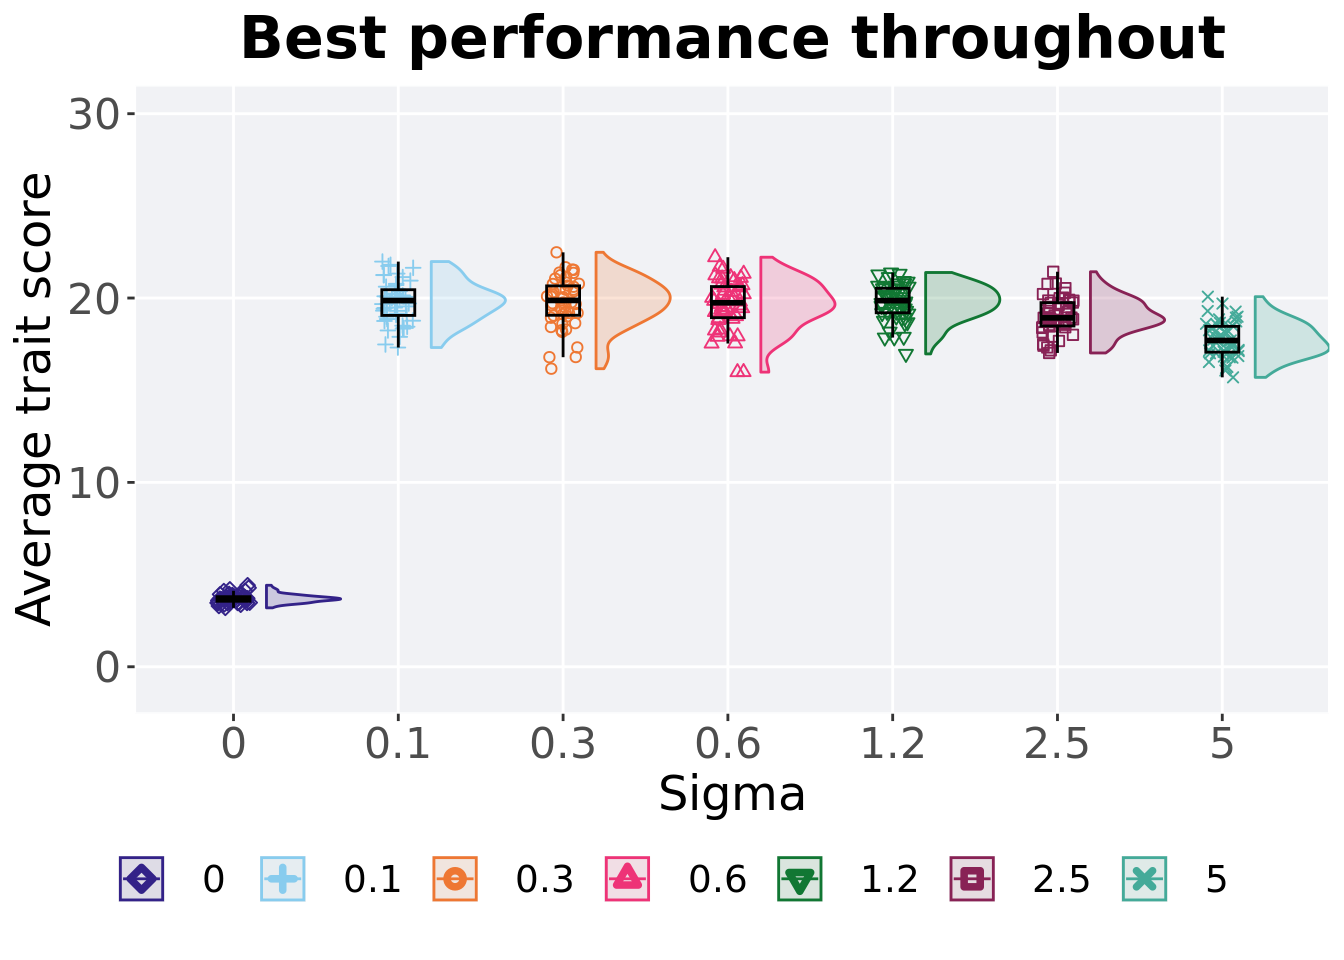
\includegraphics{demo_files/figure-latex/unnamed-chunk-151-1.pdf}

\hypertarget{best-performance-throughout-6}{%
\subsection{Best performance throughout}\label{best-performance-throughout-6}}

The best performance found throughout 50,000 generations.

\begin{Shaded}
\begin{Highlighting}[]
\NormalTok{best =}\StringTok{ }\KeywordTok{filter}\NormalTok{(gfs_best, col }\OperatorTok{==}\StringTok{ 'pop_fit_max'} \OperatorTok{&}\StringTok{ }\NormalTok{diagnostic }\OperatorTok{==}\StringTok{ 'ordered_exploitation'}\NormalTok{)}

\NormalTok{plot =}\StringTok{ }\KeywordTok{ggplot}\NormalTok{(best, }\KeywordTok{aes}\NormalTok{(}\DataTypeTok{x =}\NormalTok{ Sigma, }\DataTypeTok{y =}\NormalTok{ val }\OperatorTok{/}\StringTok{ }\NormalTok{TRAITS, }\DataTypeTok{color =}\NormalTok{ Sigma, }\DataTypeTok{fill =}\NormalTok{ Sigma, }\DataTypeTok{shape =}\NormalTok{ Sigma)) }\OperatorTok{+}
\StringTok{  }\KeywordTok{geom_flat_violin}\NormalTok{(}\DataTypeTok{position =} \KeywordTok{position_nudge}\NormalTok{(}\DataTypeTok{x =} \FloatTok{.2}\NormalTok{, }\DataTypeTok{y =} \DecValTok{0}\NormalTok{), }\DataTypeTok{scale =} \StringTok{'width'}\NormalTok{, }\DataTypeTok{alpha =} \FloatTok{0.2}\NormalTok{) }\OperatorTok{+}
\StringTok{  }\KeywordTok{geom_point}\NormalTok{(}\DataTypeTok{position =} \KeywordTok{position_jitter}\NormalTok{(}\DataTypeTok{width =} \FloatTok{.1}\NormalTok{), }\DataTypeTok{size =} \FloatTok{1.5}\NormalTok{, }\DataTypeTok{alpha =} \FloatTok{1.0}\NormalTok{) }\OperatorTok{+}
\StringTok{  }\KeywordTok{geom_boxplot}\NormalTok{(}\DataTypeTok{color =} \StringTok{'black'}\NormalTok{, }\DataTypeTok{width =} \FloatTok{.2}\NormalTok{, }\DataTypeTok{outlier.shape =} \OtherTok{NA}\NormalTok{, }\DataTypeTok{alpha =} \FloatTok{0.0}\NormalTok{) }\OperatorTok{+}
\StringTok{  }\KeywordTok{scale_y_continuous}\NormalTok{(}
    \DataTypeTok{name=}\StringTok{"Average trait score"}\NormalTok{,}
    \DataTypeTok{limits=}\KeywordTok{c}\NormalTok{(}\OperatorTok{-}\DecValTok{1}\NormalTok{, }\DecValTok{30}\NormalTok{),}
    \DataTypeTok{breaks=}\KeywordTok{seq}\NormalTok{(}\DecValTok{0}\NormalTok{, }\DecValTok{30}\NormalTok{, }\DecValTok{10}\NormalTok{),}
    \DataTypeTok{labels=}\KeywordTok{c}\NormalTok{(}\StringTok{"0"}\NormalTok{, }\StringTok{"10"}\NormalTok{, }\StringTok{"20"}\NormalTok{, }\StringTok{"30"}\NormalTok{)}
\NormalTok{  ) }\OperatorTok{+}
\StringTok{  }\KeywordTok{scale_x_discrete}\NormalTok{(}
    \DataTypeTok{name=}\StringTok{"Sigma"}
\NormalTok{  )}\OperatorTok{+}
\StringTok{  }\KeywordTok{scale_shape_manual}\NormalTok{(}\DataTypeTok{values =}\NormalTok{ SHAPE)}\OperatorTok{+}
\StringTok{  }\KeywordTok{scale_colour_manual}\NormalTok{(}\DataTypeTok{values =}\NormalTok{ cb_palette) }\OperatorTok{+}
\StringTok{  }\KeywordTok{scale_fill_manual}\NormalTok{(}\DataTypeTok{values =}\NormalTok{ cb_palette) }\OperatorTok{+}
\StringTok{  }\NormalTok{p_theme}

\KeywordTok{plot_grid}\NormalTok{(}
\NormalTok{  plot }\OperatorTok{+}
\StringTok{    }\KeywordTok{ggtitle}\NormalTok{(}\StringTok{"Best performance throughout"}\NormalTok{) }\OperatorTok{+}
\StringTok{    }\KeywordTok{theme}\NormalTok{(}\DataTypeTok{legend.position=}\StringTok{"none"}\NormalTok{),}
\NormalTok{  legend,}
  \DataTypeTok{nrow=}\DecValTok{2}\NormalTok{,}
  \DataTypeTok{rel_heights =} \KeywordTok{c}\NormalTok{(}\DecValTok{2}\NormalTok{,.}\DecValTok{2}\NormalTok{),}
  \DataTypeTok{label_size =}\NormalTok{ TSIZE}
\NormalTok{)}
\end{Highlighting}
\end{Shaded}

\includegraphics{demo_files/figure-latex/unnamed-chunk-153-1.pdf}

\hypertarget{stats-29}{%
\subsubsection{Stats}\label{stats-29}}

Summary statistics about the best performance found.

\begin{Shaded}
\begin{Highlighting}[]
\KeywordTok{group_by}\NormalTok{(best, Sigma) }\OperatorTok
\StringTok{  }\NormalTok{dplyr}\OperatorTok{::}\KeywordTok{summarise}\NormalTok{(}
    \DataTypeTok{count =} \KeywordTok{n}\NormalTok{(),}
    \DataTypeTok{na_cnt =} \KeywordTok{sum}\NormalTok{(}\KeywordTok{is.na}\NormalTok{(val)),}
    \DataTypeTok{min =} \KeywordTok{min}\NormalTok{(val }\OperatorTok{/}\StringTok{ }\NormalTok{TRAITS, }\DataTypeTok{na.rm =} \OtherTok{TRUE}\NormalTok{),}
    \DataTypeTok{median =} \KeywordTok{median}\NormalTok{(val }\OperatorTok{/}\StringTok{ }\NormalTok{TRAITS, }\DataTypeTok{na.rm =} \OtherTok{TRUE}\NormalTok{),}
    \DataTypeTok{mean =} \KeywordTok{mean}\NormalTok{(val }\OperatorTok{/}\StringTok{ }\NormalTok{TRAITS, }\DataTypeTok{na.rm =} \OtherTok{TRUE}\NormalTok{),}
    \DataTypeTok{max =} \KeywordTok{max}\NormalTok{(val }\OperatorTok{/}\StringTok{ }\NormalTok{TRAITS, }\DataTypeTok{na.rm =} \OtherTok{TRUE}\NormalTok{),}
    \DataTypeTok{IQR =} \KeywordTok{IQR}\NormalTok{(val }\OperatorTok{/}\StringTok{ }\NormalTok{TRAITS, }\DataTypeTok{na.rm =} \OtherTok{TRUE}\NormalTok{)}
\NormalTok{  )}
\end{Highlighting}
\end{Shaded}

\begin{verbatim}
## # A tibble: 7 x 8
##   Sigma count na_cnt   min median  mean   max   IQR
##   <fct> <int>  <int> <dbl>  <dbl> <dbl> <dbl> <dbl>
## 1 0        50      0  21.9   23.6  23.6  25.2 0.531
## 2 0.1      50      0  20.3   21.3  21.4  22.7 0.841
## 3 0.3      50      0  19.6   21.0  20.9  22.1 0.686
## 4 0.6      50      0  19.2   20.3  20.3  22.0 0.660
## 5 1.2      50      0  16.8   18.2  18.2  19.3 0.717
## 6 2.5      50      0  12.5   15.3  15.2  17.0 1.01 
## 7 5        50      0  13.5   14.6  14.6  15.9 0.654
\end{verbatim}

Kruskal--Wallis test provides evidence of statistical differences for the best performance found in the pouplation throughout 50,000 generations.

\begin{Shaded}
\begin{Highlighting}[]
\KeywordTok{kruskal.test}\NormalTok{(val }\OperatorTok{~}\StringTok{ }\NormalTok{Sigma,}\DataTypeTok{data =}\NormalTok{ best)}
\end{Highlighting}
\end{Shaded}

\begin{verbatim}
## 
##  Kruskal-Wallis rank sum test
## 
## data:  val by Sigma
## Kruskal-Wallis chi-squared = 325.01, df = 6, p-value < 2.2e-16
\end{verbatim}

Results for post-hoc Wilcoxon rank-sum test with a Bonferroni correction on the best performance found in the pouplation throughout 50,000 generations.

\begin{Shaded}
\begin{Highlighting}[]
\KeywordTok{pairwise.wilcox.test}\NormalTok{(}\DataTypeTok{x =}\NormalTok{ best}\OperatorTok{$}\NormalTok{val, }\DataTypeTok{g =}\NormalTok{ best}\OperatorTok{$}\NormalTok{Sigma , }\DataTypeTok{p.adjust.method =} \StringTok{"bonferroni"}\NormalTok{,}
                     \DataTypeTok{paired =} \OtherTok{FALSE}\NormalTok{, }\DataTypeTok{conf.int =} \OtherTok{FALSE}\NormalTok{, }\DataTypeTok{alternative =} \StringTok{'l'}\NormalTok{)}
\end{Highlighting}
\end{Shaded}

\begin{verbatim}
## 
##  Pairwise comparisons using Wilcoxon rank sum test with continuity correction 
## 
## data:  best$val and best$Sigma 
## 
##     0       0.1     0.3     0.6     1.2     2.5    
## 0.1 < 2e-16 -       -       -       -       -      
## 0.3 < 2e-16 0.00086 -       -       -       -      
## 0.6 < 2e-16 6.2e-13 2.5e-06 -       -       -      
## 1.2 < 2e-16 < 2e-16 < 2e-16 < 2e-16 -       -      
## 2.5 < 2e-16 < 2e-16 < 2e-16 < 2e-16 < 2e-16 -      
## 5   < 2e-16 < 2e-16 < 2e-16 < 2e-16 < 2e-16 2.6e-05
## 
## P value adjustment method: bonferroni
\end{verbatim}

\hypertarget{contraditory-objectives-diagnostic-1}{%
\section{Contraditory objectives diagnostic}\label{contraditory-objectives-diagnostic-1}}

Here we present the results for \textbf{satisfactory trait coverage} and \textbf{activation gene coverage} found by each genotypic fitness sharing sigma value replicate on the ordered exploitation diagnostic.
Satisfactory trait coverage refers to the count of unique satisfied traits in the population, while activation gene coverage refers to the count of unique activation genes in the population.
Note that both coverage values fall between 0 and 100.

\hypertarget{satisfactory-trait-coverage-2}{%
\subsection{Satisfactory trait coverage}\label{satisfactory-trait-coverage-2}}

Satisfactory trait coverage analysis.

\hypertarget{coverage-over-time-8}{%
\subsubsection{Coverage over time}\label{coverage-over-time-8}}

Satisfactory trait coverage over time.

\begin{Shaded}
\begin{Highlighting}[]
\NormalTok{problem <-}\StringTok{ }\KeywordTok{filter}\NormalTok{(gfs_ot, diagnostic }\OperatorTok{==}\StringTok{ 'contradictory_objectives'}\NormalTok{)}
\NormalTok{lines =}\StringTok{ }\NormalTok{problem }\OperatorTok
\StringTok{        }\KeywordTok{group_by}\NormalTok{(Sigma, gen) }\OperatorTok
\StringTok{          }\NormalTok{dplyr}\OperatorTok{::}\KeywordTok{summarise}\NormalTok{(}
            \DataTypeTok{min =} \KeywordTok{min}\NormalTok{(pop_uni_obj),}
            \DataTypeTok{mean =} \KeywordTok{mean}\NormalTok{(pop_uni_obj),}
            \DataTypeTok{max =} \KeywordTok{max}\NormalTok{(pop_uni_obj)}
\NormalTok{          )}
\end{Highlighting}
\end{Shaded}

\begin{verbatim}
## `summarise()` has grouped output by 'Sigma'. You can override using the
## `.groups` argument.
\end{verbatim}

\begin{Shaded}
\begin{Highlighting}[]
\NormalTok{points =}\StringTok{ }\KeywordTok{filter}\NormalTok{(lines, gen }\OperatorTok\StringTok{ }\DecValTok{2000} \OperatorTok{==}\StringTok{ }\DecValTok{0} \OperatorTok{&}\StringTok{ }\NormalTok{gen }\OperatorTok{!=}\StringTok{ }\DecValTok{0}\NormalTok{)}

\NormalTok{ot =}\StringTok{ }\KeywordTok{ggplot}\NormalTok{(lines, }\KeywordTok{aes}\NormalTok{(}\DataTypeTok{x=}\NormalTok{gen, }\DataTypeTok{y=}\NormalTok{mean, }\DataTypeTok{group =}\NormalTok{ Sigma, }\DataTypeTok{fill =}\NormalTok{Sigma, }\DataTypeTok{color =}\NormalTok{ Sigma, }\DataTypeTok{shape =}\NormalTok{ Sigma)) }\OperatorTok{+}
\StringTok{  }\KeywordTok{geom_ribbon}\NormalTok{(}\KeywordTok{aes}\NormalTok{(}\DataTypeTok{ymin =}\NormalTok{ min, }\DataTypeTok{ymax =}\NormalTok{ max), }\DataTypeTok{alpha =} \FloatTok{0.1}\NormalTok{) }\OperatorTok{+}
\StringTok{  }\KeywordTok{geom_line}\NormalTok{(}\DataTypeTok{size =} \FloatTok{0.5}\NormalTok{) }\OperatorTok{+}
\StringTok{  }\KeywordTok{geom_point}\NormalTok{(}\DataTypeTok{data =}\NormalTok{ points, }\DataTypeTok{size =} \FloatTok{1.5}\NormalTok{, }\DataTypeTok{stroke =} \FloatTok{2.0}\NormalTok{, }\DataTypeTok{alpha =} \FloatTok{1.0}\NormalTok{) }\OperatorTok{+}
\StringTok{  }\KeywordTok{scale_y_continuous}\NormalTok{(}
    \DataTypeTok{name=}\StringTok{"Coverage"}\NormalTok{,}
    \DataTypeTok{limits=}\KeywordTok{c}\NormalTok{(}\DecValTok{0}\NormalTok{, }\DecValTok{5}\NormalTok{)}
\NormalTok{  ) }\OperatorTok{+}
\StringTok{  }\KeywordTok{scale_x_continuous}\NormalTok{(}
    \DataTypeTok{name=}\StringTok{"Generations"}\NormalTok{,}
    \DataTypeTok{limits=}\KeywordTok{c}\NormalTok{(}\DecValTok{0}\NormalTok{, }\DecValTok{50000}\NormalTok{),}
    \DataTypeTok{breaks=}\KeywordTok{c}\NormalTok{(}\DecValTok{0}\NormalTok{, }\DecValTok{10000}\NormalTok{, }\DecValTok{20000}\NormalTok{, }\DecValTok{30000}\NormalTok{, }\DecValTok{40000}\NormalTok{, }\DecValTok{50000}\NormalTok{),}
    \DataTypeTok{labels=}\KeywordTok{c}\NormalTok{(}\StringTok{"0e+6"}\NormalTok{, }\StringTok{"1e+6"}\NormalTok{, }\StringTok{"2e+6"}\NormalTok{, }\StringTok{"3e+6"}\NormalTok{, }\StringTok{"4e+6"}\NormalTok{, }\StringTok{"5e+6"}\NormalTok{)}

\NormalTok{  ) }\OperatorTok{+}
\StringTok{  }\KeywordTok{scale_shape_manual}\NormalTok{(}\DataTypeTok{values=}\NormalTok{SHAPE)}\OperatorTok{+}
\StringTok{  }\KeywordTok{scale_colour_manual}\NormalTok{(}\DataTypeTok{values =}\NormalTok{ cb_palette) }\OperatorTok{+}
\StringTok{  }\KeywordTok{scale_fill_manual}\NormalTok{(}\DataTypeTok{values =}\NormalTok{ cb_palette) }\OperatorTok{+}
\StringTok{  }\KeywordTok{ggtitle}\NormalTok{(}\StringTok{"Satisfactory trait coverage over time"}\NormalTok{) }\OperatorTok{+}
\StringTok{  }\NormalTok{p_theme}\OperatorTok{+}
\StringTok{    }\KeywordTok{guides}\NormalTok{(}
    \DataTypeTok{shape=}\KeywordTok{guide_legend}\NormalTok{(}\DataTypeTok{nrow=}\DecValTok{1}\NormalTok{, }\DataTypeTok{title.position =} \StringTok{"bottom"}\NormalTok{),}
    \DataTypeTok{color=}\KeywordTok{guide_legend}\NormalTok{(}\DataTypeTok{nrow=}\DecValTok{1}\NormalTok{, }\DataTypeTok{title.position =} \StringTok{"bottom"}\NormalTok{),}
    \DataTypeTok{fill=}\KeywordTok{guide_legend}\NormalTok{(}\DataTypeTok{nrow=}\DecValTok{1}\NormalTok{, }\DataTypeTok{title.position =} \StringTok{"bottom"}\NormalTok{)}
\NormalTok{  ) }\OperatorTok{+}
\StringTok{  }\KeywordTok{theme}\NormalTok{(}
    \DataTypeTok{legend.position =} \StringTok{"bottom"}\NormalTok{,}
    \DataTypeTok{legend.box=}\StringTok{"verticle"}\NormalTok{,}
    \DataTypeTok{legend.justification=}\StringTok{"center"}\NormalTok{,}
    \DataTypeTok{legend.title.align=}\FloatTok{0.5}
\NormalTok{  )}

\NormalTok{ot}
\end{Highlighting}
\end{Shaded}

\includegraphics{demo_files/figure-latex/unnamed-chunk-157-1.pdf}

\hypertarget{best-coverage-throughout-4}{%
\subsubsection{Best coverage throughout}\label{best-coverage-throughout-4}}

Best satisfactory trait coverage throughout 50,000 generations.

\begin{Shaded}
\begin{Highlighting}[]
\NormalTok{best =}\StringTok{ }\KeywordTok{filter}\NormalTok{(gfs_best, col }\OperatorTok{==}\StringTok{ 'pop_uni_obj'} \OperatorTok{&}\StringTok{ }\NormalTok{diagnostic }\OperatorTok{==}\StringTok{ 'contradictory_objectives'}\NormalTok{)}

\NormalTok{plot =}\StringTok{ }\KeywordTok{ggplot}\NormalTok{(best, }\KeywordTok{aes}\NormalTok{(}\DataTypeTok{x =}\NormalTok{ Sigma, }\DataTypeTok{y =}\NormalTok{ val, }\DataTypeTok{color =}\NormalTok{ Sigma, }\DataTypeTok{fill =}\NormalTok{ Sigma, }\DataTypeTok{shape =}\NormalTok{ Sigma)) }\OperatorTok{+}
\StringTok{  }\KeywordTok{geom_flat_violin}\NormalTok{(}\DataTypeTok{position =} \KeywordTok{position_nudge}\NormalTok{(}\DataTypeTok{x =} \FloatTok{.2}\NormalTok{, }\DataTypeTok{y =} \DecValTok{0}\NormalTok{), }\DataTypeTok{scale =} \StringTok{'width'}\NormalTok{, }\DataTypeTok{alpha =} \FloatTok{0.2}\NormalTok{) }\OperatorTok{+}
\StringTok{  }\KeywordTok{geom_point}\NormalTok{(}\DataTypeTok{position =} \KeywordTok{position_jitter}\NormalTok{(}\DataTypeTok{width =} \FloatTok{.1}\NormalTok{), }\DataTypeTok{size =} \FloatTok{1.5}\NormalTok{, }\DataTypeTok{alpha =} \FloatTok{1.0}\NormalTok{) }\OperatorTok{+}
\StringTok{  }\KeywordTok{geom_boxplot}\NormalTok{(}\DataTypeTok{color =} \StringTok{'black'}\NormalTok{, }\DataTypeTok{width =} \FloatTok{.2}\NormalTok{, }\DataTypeTok{outlier.shape =} \OtherTok{NA}\NormalTok{, }\DataTypeTok{alpha =} \FloatTok{0.0}\NormalTok{) }\OperatorTok{+}
\StringTok{  }\KeywordTok{scale_y_continuous}\NormalTok{(}
    \DataTypeTok{name=}\StringTok{"Coverage"}\NormalTok{,}
    \DataTypeTok{limits=}\KeywordTok{c}\NormalTok{(}\DecValTok{0}\NormalTok{, }\DecValTok{5}\NormalTok{)}
\NormalTok{  ) }\OperatorTok{+}
\StringTok{  }\KeywordTok{scale_x_discrete}\NormalTok{(}
    \DataTypeTok{name=}\StringTok{"Sigma"}
\NormalTok{  )}\OperatorTok{+}
\StringTok{  }\KeywordTok{scale_shape_manual}\NormalTok{(}\DataTypeTok{values=}\NormalTok{SHAPE)}\OperatorTok{+}
\StringTok{  }\KeywordTok{scale_colour_manual}\NormalTok{(}\DataTypeTok{values =}\NormalTok{ cb_palette) }\OperatorTok{+}
\StringTok{  }\KeywordTok{scale_fill_manual}\NormalTok{(}\DataTypeTok{values =}\NormalTok{ cb_palette) }\OperatorTok{+}
\StringTok{  }\NormalTok{p_theme}

\KeywordTok{plot_grid}\NormalTok{(}
\NormalTok{  plot }\OperatorTok{+}
\StringTok{    }\KeywordTok{ggtitle}\NormalTok{(}\StringTok{"Best satisfactory trait coverage"}\NormalTok{) }\OperatorTok{+}
\StringTok{    }\KeywordTok{theme}\NormalTok{(}\DataTypeTok{legend.position=}\StringTok{"none"}\NormalTok{),}
\NormalTok{  legend,}
  \DataTypeTok{nrow=}\DecValTok{2}\NormalTok{,}
  \DataTypeTok{rel_heights =} \KeywordTok{c}\NormalTok{(}\DecValTok{2}\NormalTok{,.}\DecValTok{2}\NormalTok{),}
  \DataTypeTok{label_size =}\NormalTok{ TSIZE}
\NormalTok{)}
\end{Highlighting}
\end{Shaded}

\includegraphics{demo_files/figure-latex/unnamed-chunk-159-1.pdf}

\hypertarget{stats-30}{%
\paragraph{Stats}\label{stats-30}}

Summary statistics for the best satisfactory trait coverage throughout 50,000 generations.

\begin{Shaded}
\begin{Highlighting}[]
\KeywordTok{group_by}\NormalTok{(best, Sigma) }\OperatorTok
\StringTok{  }\NormalTok{dplyr}\OperatorTok{::}\KeywordTok{summarise}\NormalTok{(}
    \DataTypeTok{count =} \KeywordTok{n}\NormalTok{(),}
    \DataTypeTok{na_cnt =} \KeywordTok{sum}\NormalTok{(}\KeywordTok{is.na}\NormalTok{(val)),}
    \DataTypeTok{min =} \KeywordTok{min}\NormalTok{(val, }\DataTypeTok{na.rm =} \OtherTok{TRUE}\NormalTok{),}
    \DataTypeTok{median =} \KeywordTok{median}\NormalTok{(val, }\DataTypeTok{na.rm =} \OtherTok{TRUE}\NormalTok{),}
    \DataTypeTok{mean =} \KeywordTok{mean}\NormalTok{(val, }\DataTypeTok{na.rm =} \OtherTok{TRUE}\NormalTok{),}
    \DataTypeTok{max =} \KeywordTok{max}\NormalTok{(val, }\DataTypeTok{na.rm =} \OtherTok{TRUE}\NormalTok{),}
    \DataTypeTok{IQR =} \KeywordTok{IQR}\NormalTok{(val, }\DataTypeTok{na.rm =} \OtherTok{TRUE}\NormalTok{)}
\NormalTok{  )}
\end{Highlighting}
\end{Shaded}

\begin{verbatim}
## # A tibble: 7 x 8
##   Sigma count na_cnt   min median  mean   max   IQR
##   <fct> <int>  <int> <dbl>  <dbl> <dbl> <dbl> <dbl>
## 1 0        50      0     1      1  1        1     0
## 2 0.1      50      0     1      1  1        1     0
## 3 0.3      50      0     1      1  1        1     0
## 4 0.6      50      0     1      1  1.02     2     0
## 5 1.2      50      0     1      1  1        1     0
## 6 2.5      50      0     1      1  1        1     0
## 7 5        50      0     1      1  1        1     0
\end{verbatim}

Kruskal--Wallis test provides evidence of no statistical difference among satisfactory trait coverage throughout 50,000 generations.

\begin{Shaded}
\begin{Highlighting}[]
\KeywordTok{kruskal.test}\NormalTok{(val }\OperatorTok{~}\StringTok{ }\NormalTok{Sigma, }\DataTypeTok{data =}\NormalTok{ best)}
\end{Highlighting}
\end{Shaded}

\begin{verbatim}
## 
##  Kruskal-Wallis rank sum test
## 
## data:  val by Sigma
## Kruskal-Wallis chi-squared = 6, df = 6, p-value = 0.4232
\end{verbatim}

\hypertarget{end-of-50000-generations-13}{%
\subsubsection{End of 50,000 generations}\label{end-of-50000-generations-13}}

Satisfactory trait coverage in the population at the end of 50,000 generations.

\begin{Shaded}
\begin{Highlighting}[]
\NormalTok{end =}\StringTok{ }\KeywordTok{filter}\NormalTok{(gfs_end, diagnostic }\OperatorTok{==}\StringTok{ 'contradictory_objectives'}\NormalTok{)}
\NormalTok{plot =}\StringTok{ }\KeywordTok{ggplot}\NormalTok{(end, }\KeywordTok{aes}\NormalTok{(}\DataTypeTok{x =}\NormalTok{ Sigma, }\DataTypeTok{y =}\NormalTok{ pop_uni_obj, }\DataTypeTok{color =}\NormalTok{ Sigma, }\DataTypeTok{fill =}\NormalTok{ Sigma, }\DataTypeTok{shape =}\NormalTok{ Sigma)) }\OperatorTok{+}
\StringTok{  }\KeywordTok{geom_flat_violin}\NormalTok{(}\DataTypeTok{position =} \KeywordTok{position_nudge}\NormalTok{(}\DataTypeTok{x =} \FloatTok{.2}\NormalTok{, }\DataTypeTok{y =} \DecValTok{0}\NormalTok{), }\DataTypeTok{scale =} \StringTok{'width'}\NormalTok{, }\DataTypeTok{alpha =} \FloatTok{0.2}\NormalTok{) }\OperatorTok{+}
\StringTok{  }\KeywordTok{geom_point}\NormalTok{(}\DataTypeTok{position =} \KeywordTok{position_jitter}\NormalTok{(}\DataTypeTok{width =} \FloatTok{.1}\NormalTok{), }\DataTypeTok{size =} \FloatTok{1.5}\NormalTok{, }\DataTypeTok{alpha =} \FloatTok{1.0}\NormalTok{) }\OperatorTok{+}
\StringTok{  }\KeywordTok{geom_boxplot}\NormalTok{(}\DataTypeTok{color =} \StringTok{'black'}\NormalTok{, }\DataTypeTok{width =} \FloatTok{.2}\NormalTok{, }\DataTypeTok{outlier.shape =} \OtherTok{NA}\NormalTok{, }\DataTypeTok{alpha =} \FloatTok{0.0}\NormalTok{) }\OperatorTok{+}
\StringTok{  }\KeywordTok{scale_y_continuous}\NormalTok{(}
    \DataTypeTok{name=}\StringTok{"Coverage"}\NormalTok{,}
    \DataTypeTok{limits=}\KeywordTok{c}\NormalTok{(}\DecValTok{0}\NormalTok{, }\DecValTok{5}\NormalTok{)}
\NormalTok{  ) }\OperatorTok{+}
\StringTok{  }\KeywordTok{scale_x_discrete}\NormalTok{(}
    \DataTypeTok{name=}\StringTok{"Sigma"}
\NormalTok{  )}\OperatorTok{+}
\StringTok{  }\KeywordTok{scale_shape_manual}\NormalTok{(}\DataTypeTok{values=}\NormalTok{SHAPE)}\OperatorTok{+}
\StringTok{  }\KeywordTok{scale_colour_manual}\NormalTok{(}\DataTypeTok{values =}\NormalTok{ cb_palette) }\OperatorTok{+}
\StringTok{  }\KeywordTok{scale_fill_manual}\NormalTok{(}\DataTypeTok{values =}\NormalTok{ cb_palette) }\OperatorTok{+}
\StringTok{  }\NormalTok{p_theme}

\KeywordTok{plot_grid}\NormalTok{(}
\NormalTok{  plot }\OperatorTok{+}
\StringTok{    }\KeywordTok{ggtitle}\NormalTok{(}\StringTok{"Final satisfactory trait coverage"}\NormalTok{) }\OperatorTok{+}
\StringTok{    }\KeywordTok{theme}\NormalTok{(}\DataTypeTok{legend.position=}\StringTok{"none"}\NormalTok{),}
\NormalTok{  legend,}
  \DataTypeTok{nrow=}\DecValTok{2}\NormalTok{,}
  \DataTypeTok{rel_heights =} \KeywordTok{c}\NormalTok{(}\DecValTok{2}\NormalTok{,.}\DecValTok{3}\NormalTok{),}
  \DataTypeTok{label_size =}\NormalTok{ TSIZE}
\NormalTok{)}
\end{Highlighting}
\end{Shaded}

\includegraphics{demo_files/figure-latex/unnamed-chunk-162-1.pdf}

\hypertarget{stats-31}{%
\paragraph{Stats}\label{stats-31}}

Summary statistics for satisfactory trait coverage in the population at the end of 50,000 generations.

\begin{Shaded}
\begin{Highlighting}[]
\KeywordTok{group_by}\NormalTok{(end, Sigma) }\OperatorTok
\StringTok{  }\NormalTok{dplyr}\OperatorTok{::}\KeywordTok{summarise}\NormalTok{(}
    \DataTypeTok{count =} \KeywordTok{n}\NormalTok{(),}
    \DataTypeTok{na_cnt =} \KeywordTok{sum}\NormalTok{(}\KeywordTok{is.na}\NormalTok{(pop_uni_obj)),}
    \DataTypeTok{min =} \KeywordTok{min}\NormalTok{(pop_uni_obj, }\DataTypeTok{na.rm =} \OtherTok{TRUE}\NormalTok{),}
    \DataTypeTok{median =} \KeywordTok{median}\NormalTok{(pop_uni_obj, }\DataTypeTok{na.rm =} \OtherTok{TRUE}\NormalTok{),}
    \DataTypeTok{mean =} \KeywordTok{mean}\NormalTok{(pop_uni_obj, }\DataTypeTok{na.rm =} \OtherTok{TRUE}\NormalTok{),}
    \DataTypeTok{max =} \KeywordTok{max}\NormalTok{(pop_uni_obj, }\DataTypeTok{na.rm =} \OtherTok{TRUE}\NormalTok{),}
    \DataTypeTok{IQR =} \KeywordTok{IQR}\NormalTok{(pop_uni_obj, }\DataTypeTok{na.rm =} \OtherTok{TRUE}\NormalTok{)}
\NormalTok{  )}
\end{Highlighting}
\end{Shaded}

\begin{verbatim}
## # A tibble: 7 x 8
##   Sigma count na_cnt   min median  mean   max   IQR
##   <fct> <int>  <int> <int>  <dbl> <dbl> <int> <dbl>
## 1 0        50      0     1      1  1        1     0
## 2 0.1      50      0     1      1  1        1     0
## 3 0.3      50      0     1      1  1        1     0
## 4 0.6      50      0     1      1  1.02     2     0
## 5 1.2      50      0     1      1  1        1     0
## 6 2.5      50      0     1      1  1        1     0
## 7 5        50      0     1      1  1        1     0
\end{verbatim}

Kruskal--Wallis test provides evidence of no statistical difference among satisfactory trait coverage throughout 50,000 generations.

\begin{Shaded}
\begin{Highlighting}[]
\KeywordTok{kruskal.test}\NormalTok{(pop_uni_obj }\OperatorTok{~}\StringTok{ }\NormalTok{Sigma, }\DataTypeTok{data =}\NormalTok{ end)}
\end{Highlighting}
\end{Shaded}

\begin{verbatim}
## 
##  Kruskal-Wallis rank sum test
## 
## data:  pop_uni_obj by Sigma
## Kruskal-Wallis chi-squared = 6, df = 6, p-value = 0.4232
\end{verbatim}

\hypertarget{activation-gene-coverage-6}{%
\subsection{Activation gene coverage}\label{activation-gene-coverage-6}}

Here we analyze the activation gene coverage for each parameter replicate on the contradictory objectives diagnostic.

\hypertarget{coverage-over-time-9}{%
\subsubsection{Coverage over time}\label{coverage-over-time-9}}

Activation gene coverage over time.

\begin{Shaded}
\begin{Highlighting}[]
\NormalTok{problem <-}\StringTok{ }\KeywordTok{filter}\NormalTok{(gfs_ot, diagnostic }\OperatorTok{==}\StringTok{ 'contradictory_objectives'}\NormalTok{)}
\NormalTok{lines =}\StringTok{ }\NormalTok{problem }\OperatorTok
\StringTok{        }\KeywordTok{group_by}\NormalTok{(Sigma, gen) }\OperatorTok
\StringTok{          }\NormalTok{dplyr}\OperatorTok{::}\KeywordTok{summarise}\NormalTok{(}
            \DataTypeTok{min =} \KeywordTok{min}\NormalTok{(uni_str_pos),}
            \DataTypeTok{mean =} \KeywordTok{mean}\NormalTok{(uni_str_pos),}
            \DataTypeTok{max =} \KeywordTok{max}\NormalTok{(uni_str_pos)}
\NormalTok{          )}
\end{Highlighting}
\end{Shaded}

\begin{verbatim}
## `summarise()` has grouped output by 'Sigma'. You can override using the
## `.groups` argument.
\end{verbatim}

\begin{Shaded}
\begin{Highlighting}[]
\NormalTok{points =}\StringTok{ }\KeywordTok{filter}\NormalTok{(lines, gen }\OperatorTok\StringTok{ }\DecValTok{2000} \OperatorTok{==}\StringTok{ }\DecValTok{0} \OperatorTok{&}\StringTok{ }\NormalTok{gen }\OperatorTok{!=}\StringTok{ }\DecValTok{0}\NormalTok{)}

\NormalTok{ot =}\StringTok{ }\KeywordTok{ggplot}\NormalTok{(lines, }\KeywordTok{aes}\NormalTok{(}\DataTypeTok{x=}\NormalTok{gen, }\DataTypeTok{y=}\NormalTok{mean, }\DataTypeTok{group =}\NormalTok{ Sigma, }\DataTypeTok{fill =}\NormalTok{Sigma, }\DataTypeTok{color =}\NormalTok{ Sigma, }\DataTypeTok{shape =}\NormalTok{ Sigma)) }\OperatorTok{+}
\StringTok{  }\KeywordTok{geom_ribbon}\NormalTok{(}\KeywordTok{aes}\NormalTok{(}\DataTypeTok{ymin =}\NormalTok{ min, }\DataTypeTok{ymax =}\NormalTok{ max), }\DataTypeTok{alpha =} \FloatTok{0.1}\NormalTok{) }\OperatorTok{+}
\StringTok{  }\KeywordTok{geom_line}\NormalTok{(}\DataTypeTok{size =} \FloatTok{0.5}\NormalTok{) }\OperatorTok{+}
\StringTok{  }\KeywordTok{geom_point}\NormalTok{(}\DataTypeTok{data =}\NormalTok{ points, }\DataTypeTok{size =} \FloatTok{1.5}\NormalTok{, }\DataTypeTok{stroke =} \FloatTok{2.0}\NormalTok{, }\DataTypeTok{alpha =} \FloatTok{1.0}\NormalTok{) }\OperatorTok{+}
\StringTok{  }\KeywordTok{scale_y_continuous}\NormalTok{(}
    \DataTypeTok{name=}\StringTok{"Coverage"}\NormalTok{,}
    \DataTypeTok{limits=}\KeywordTok{c}\NormalTok{(}\OperatorTok{-}\DecValTok{1}\NormalTok{, }\DecValTok{101}\NormalTok{),}
    \DataTypeTok{breaks=}\KeywordTok{seq}\NormalTok{(}\DecValTok{0}\NormalTok{,}\DecValTok{100}\NormalTok{, }\DecValTok{20}\NormalTok{),}
    \DataTypeTok{labels=}\KeywordTok{c}\NormalTok{(}\StringTok{"0"}\NormalTok{, }\StringTok{"20"}\NormalTok{, }\StringTok{"40"}\NormalTok{, }\StringTok{"60"}\NormalTok{, }\StringTok{"80"}\NormalTok{, }\StringTok{"100"}\NormalTok{)}
\NormalTok{  ) }\OperatorTok{+}
\StringTok{  }\KeywordTok{scale_x_continuous}\NormalTok{(}
    \DataTypeTok{name=}\StringTok{"Generations"}\NormalTok{,}
    \DataTypeTok{limits=}\KeywordTok{c}\NormalTok{(}\DecValTok{0}\NormalTok{, }\DecValTok{50000}\NormalTok{),}
    \DataTypeTok{breaks=}\KeywordTok{c}\NormalTok{(}\DecValTok{0}\NormalTok{, }\DecValTok{10000}\NormalTok{, }\DecValTok{20000}\NormalTok{, }\DecValTok{30000}\NormalTok{, }\DecValTok{40000}\NormalTok{, }\DecValTok{50000}\NormalTok{),}
    \DataTypeTok{labels=}\KeywordTok{c}\NormalTok{(}\StringTok{"0e+6"}\NormalTok{, }\StringTok{"1e+6"}\NormalTok{, }\StringTok{"2e+6"}\NormalTok{, }\StringTok{"3e+6"}\NormalTok{, }\StringTok{"4e+6"}\NormalTok{, }\StringTok{"5e+6"}\NormalTok{)}

\NormalTok{  ) }\OperatorTok{+}
\StringTok{  }\KeywordTok{scale_shape_manual}\NormalTok{(}\DataTypeTok{values=}\NormalTok{SHAPE)}\OperatorTok{+}
\StringTok{  }\KeywordTok{scale_colour_manual}\NormalTok{(}\DataTypeTok{values =}\NormalTok{ cb_palette) }\OperatorTok{+}
\StringTok{  }\KeywordTok{scale_fill_manual}\NormalTok{(}\DataTypeTok{values =}\NormalTok{ cb_palette) }\OperatorTok{+}
\StringTok{  }\KeywordTok{ggtitle}\NormalTok{(}\StringTok{"Activation gene coverage over time"}\NormalTok{) }\OperatorTok{+}
\StringTok{  }\NormalTok{p_theme}\OperatorTok{+}
\StringTok{    }\KeywordTok{guides}\NormalTok{(}
    \DataTypeTok{shape=}\KeywordTok{guide_legend}\NormalTok{(}\DataTypeTok{nrow=}\DecValTok{1}\NormalTok{, }\DataTypeTok{title.position =} \StringTok{"bottom"}\NormalTok{),}
    \DataTypeTok{color=}\KeywordTok{guide_legend}\NormalTok{(}\DataTypeTok{nrow=}\DecValTok{1}\NormalTok{, }\DataTypeTok{title.position =} \StringTok{"bottom"}\NormalTok{),}
    \DataTypeTok{fill=}\KeywordTok{guide_legend}\NormalTok{(}\DataTypeTok{nrow=}\DecValTok{1}\NormalTok{, }\DataTypeTok{title.position =} \StringTok{"bottom"}\NormalTok{)}
\NormalTok{  ) }\OperatorTok{+}
\StringTok{  }\KeywordTok{theme}\NormalTok{(}
    \DataTypeTok{legend.position =} \StringTok{"bottom"}\NormalTok{,}
    \DataTypeTok{legend.box=}\StringTok{"verticle"}\NormalTok{,}
    \DataTypeTok{legend.justification=}\StringTok{"center"}\NormalTok{,}
    \DataTypeTok{legend.title.align=}\FloatTok{0.5}
\NormalTok{  )}

\NormalTok{ot}
\end{Highlighting}
\end{Shaded}

\includegraphics{demo_files/figure-latex/unnamed-chunk-165-1.pdf}

\hypertarget{end-of-50000-generations-14}{%
\subsubsection{End of 50,000 generations}\label{end-of-50000-generations-14}}

Activation gene coverage in the population at the end of 50,000 generations.

\begin{Shaded}
\begin{Highlighting}[]
\NormalTok{end =}\StringTok{ }\KeywordTok{filter}\NormalTok{(gfs_end, diagnostic }\OperatorTok{==}\StringTok{ 'contradictory_objectives'}\NormalTok{)}
\NormalTok{plot =}\StringTok{ }\KeywordTok{ggplot}\NormalTok{(end, }\KeywordTok{aes}\NormalTok{(}\DataTypeTok{x =}\NormalTok{ Sigma, }\DataTypeTok{y =}\NormalTok{ uni_str_pos, }\DataTypeTok{color =}\NormalTok{ Sigma, }\DataTypeTok{fill =}\NormalTok{ Sigma, }\DataTypeTok{shape =}\NormalTok{ Sigma)) }\OperatorTok{+}
\StringTok{  }\KeywordTok{geom_flat_violin}\NormalTok{(}\DataTypeTok{position =} \KeywordTok{position_nudge}\NormalTok{(}\DataTypeTok{x =} \FloatTok{.2}\NormalTok{, }\DataTypeTok{y =} \DecValTok{0}\NormalTok{), }\DataTypeTok{scale =} \StringTok{'width'}\NormalTok{, }\DataTypeTok{alpha =} \FloatTok{0.2}\NormalTok{) }\OperatorTok{+}
\StringTok{  }\KeywordTok{geom_point}\NormalTok{(}\DataTypeTok{position =} \KeywordTok{position_jitter}\NormalTok{(}\DataTypeTok{width =} \FloatTok{.1}\NormalTok{), }\DataTypeTok{size =} \FloatTok{1.5}\NormalTok{, }\DataTypeTok{alpha =} \FloatTok{1.0}\NormalTok{) }\OperatorTok{+}
\StringTok{  }\KeywordTok{geom_boxplot}\NormalTok{(}\DataTypeTok{color =} \StringTok{'black'}\NormalTok{, }\DataTypeTok{width =} \FloatTok{.2}\NormalTok{, }\DataTypeTok{outlier.shape =} \OtherTok{NA}\NormalTok{, }\DataTypeTok{alpha =} \FloatTok{0.0}\NormalTok{) }\OperatorTok{+}
\StringTok{  }\KeywordTok{scale_y_continuous}\NormalTok{(}
    \DataTypeTok{name=}\StringTok{"Coverage"}\NormalTok{,}
    \DataTypeTok{limits=}\KeywordTok{c}\NormalTok{(}\DecValTok{0}\NormalTok{, }\DecValTok{5}\NormalTok{)}
\NormalTok{  ) }\OperatorTok{+}
\StringTok{  }\KeywordTok{scale_x_discrete}\NormalTok{(}
    \DataTypeTok{name=}\StringTok{"Sigma"}
\NormalTok{  )}\OperatorTok{+}
\StringTok{  }\KeywordTok{scale_shape_manual}\NormalTok{(}\DataTypeTok{values=}\NormalTok{SHAPE)}\OperatorTok{+}
\StringTok{  }\KeywordTok{scale_colour_manual}\NormalTok{(}\DataTypeTok{values =}\NormalTok{ cb_palette) }\OperatorTok{+}
\StringTok{  }\KeywordTok{scale_fill_manual}\NormalTok{(}\DataTypeTok{values =}\NormalTok{ cb_palette) }\OperatorTok{+}
\StringTok{  }\NormalTok{p_theme}

\KeywordTok{plot_grid}\NormalTok{(}
\NormalTok{  plot }\OperatorTok{+}
\StringTok{    }\KeywordTok{ggtitle}\NormalTok{(}\StringTok{"Final activation gene coverage"}\NormalTok{) }\OperatorTok{+}
\StringTok{    }\KeywordTok{theme}\NormalTok{(}\DataTypeTok{legend.position=}\StringTok{"none"}\NormalTok{),}
\NormalTok{  legend,}
  \DataTypeTok{nrow=}\DecValTok{2}\NormalTok{,}
  \DataTypeTok{rel_heights =} \KeywordTok{c}\NormalTok{(}\DecValTok{2}\NormalTok{,.}\DecValTok{2}\NormalTok{),}
  \DataTypeTok{label_size =}\NormalTok{ TSIZE}
\NormalTok{)}
\end{Highlighting}
\end{Shaded}

\includegraphics{demo_files/figure-latex/unnamed-chunk-166-1.pdf}

\hypertarget{stats-32}{%
\paragraph{Stats}\label{stats-32}}

Summary statistics for activation gene coverage in the population at the end of 50,000 generations.

\begin{Shaded}
\begin{Highlighting}[]
\KeywordTok{group_by}\NormalTok{(end, Sigma) }\OperatorTok
\StringTok{  }\NormalTok{dplyr}\OperatorTok{::}\KeywordTok{summarise}\NormalTok{(}
    \DataTypeTok{count =} \KeywordTok{n}\NormalTok{(),}
    \DataTypeTok{na_cnt =} \KeywordTok{sum}\NormalTok{(}\KeywordTok{is.na}\NormalTok{(uni_str_pos)),}
    \DataTypeTok{min =} \KeywordTok{min}\NormalTok{(uni_str_pos, }\DataTypeTok{na.rm =} \OtherTok{TRUE}\NormalTok{),}
    \DataTypeTok{median =} \KeywordTok{median}\NormalTok{(uni_str_pos, }\DataTypeTok{na.rm =} \OtherTok{TRUE}\NormalTok{),}
    \DataTypeTok{mean =} \KeywordTok{mean}\NormalTok{(uni_str_pos, }\DataTypeTok{na.rm =} \OtherTok{TRUE}\NormalTok{),}
    \DataTypeTok{max =} \KeywordTok{max}\NormalTok{(uni_str_pos, }\DataTypeTok{na.rm =} \OtherTok{TRUE}\NormalTok{),}
    \DataTypeTok{IQR =} \KeywordTok{IQR}\NormalTok{(uni_str_pos, }\DataTypeTok{na.rm =} \OtherTok{TRUE}\NormalTok{)}
\NormalTok{  )}
\end{Highlighting}
\end{Shaded}

\begin{verbatim}
## # A tibble: 7 x 8
##   Sigma count na_cnt   min median  mean   max   IQR
##   <fct> <int>  <int> <int>  <dbl> <dbl> <int> <dbl>
## 1 0        50      0     1      1  1        1     0
## 2 0.1      50      0     1      1  1        1     0
## 3 0.3      50      0     1      1  1        1     0
## 4 0.6      50      0     1      1  1.02     2     0
## 5 1.2      50      0     1      1  1        1     0
## 6 2.5      50      0     1      1  1        1     0
## 7 5        50      0     1      1  1        1     0
\end{verbatim}

Kruskal--Wallis test provides evidence of no statistical difference for activation gene coverage in the population at the end of 50,000 generations.

\begin{Shaded}
\begin{Highlighting}[]
\KeywordTok{kruskal.test}\NormalTok{(uni_str_pos }\OperatorTok{~}\StringTok{ }\NormalTok{Sigma,}\DataTypeTok{data =}\NormalTok{ end)}
\end{Highlighting}
\end{Shaded}

\begin{verbatim}
## 
##  Kruskal-Wallis rank sum test
## 
## data:  uni_str_pos by Sigma
## Kruskal-Wallis chi-squared = 6, df = 6, p-value = 0.4232
\end{verbatim}

\hypertarget{multi-path-exploration-results-3}{%
\section{Multi-path exploration results}\label{multi-path-exploration-results-3}}

Here we present the results for \textbf{best performances} and \textbf{activation gene coverage} found by each genotypic fitness sharing sigma value replicate on the multi-path exploration diagnostic.
Best performance found refers to the largest average trait score found in a given population, while activation gene coverage refers to the count of unique activation genes in the population.
Note that both values fall between 0 and 100.

\hypertarget{performance-3}{%
\subsection{Performance}\label{performance-3}}

Here we analyze the performances for each parameter replicate on the multi-path exploration diagnostic.

\hypertarget{performance-over-time-10}{%
\subsubsection{Performance over time}\label{performance-over-time-10}}

Performance over time.

\begin{Shaded}
\begin{Highlighting}[]
\NormalTok{problem <-}\StringTok{ }\KeywordTok{filter}\NormalTok{(gfs_ot, diagnostic }\OperatorTok{==}\StringTok{ 'multipath_exploration'}\NormalTok{)}
\NormalTok{lines =}\StringTok{ }\NormalTok{problem }\OperatorTok
\StringTok{        }\KeywordTok{group_by}\NormalTok{(Sigma, gen) }\OperatorTok
\StringTok{          }\NormalTok{dplyr}\OperatorTok{::}\KeywordTok{summarise}\NormalTok{(}
            \DataTypeTok{min =} \KeywordTok{min}\NormalTok{(pop_fit_max),}
            \DataTypeTok{mean =} \KeywordTok{mean}\NormalTok{(pop_fit_max),}
            \DataTypeTok{max =} \KeywordTok{max}\NormalTok{(pop_fit_max)}
\NormalTok{          )}
\end{Highlighting}
\end{Shaded}

\begin{verbatim}
## `summarise()` has grouped output by 'Sigma'. You can override using the
## `.groups` argument.
\end{verbatim}

\begin{Shaded}
\begin{Highlighting}[]
\NormalTok{points =}\StringTok{ }\KeywordTok{filter}\NormalTok{(lines, gen }\OperatorTok\StringTok{ }\DecValTok{2000} \OperatorTok{==}\StringTok{ }\DecValTok{0} \OperatorTok{&}\StringTok{ }\NormalTok{gen }\OperatorTok{!=}\StringTok{ }\DecValTok{0}\NormalTok{)}

\NormalTok{ot =}\StringTok{ }\KeywordTok{ggplot}\NormalTok{(lines, }\KeywordTok{aes}\NormalTok{(}\DataTypeTok{x=}\NormalTok{gen, }\DataTypeTok{y=}\NormalTok{mean }\OperatorTok{/}\StringTok{ }\NormalTok{TRAITS, }\DataTypeTok{group =}\NormalTok{ Sigma, }\DataTypeTok{fill =}\NormalTok{ Sigma, }\DataTypeTok{color =}\NormalTok{ Sigma, }\DataTypeTok{shape =}\NormalTok{ Sigma)) }\OperatorTok{+}
\StringTok{  }\KeywordTok{geom_ribbon}\NormalTok{(}\KeywordTok{aes}\NormalTok{(}\DataTypeTok{ymin =}\NormalTok{ min }\OperatorTok{/}\StringTok{ }\NormalTok{TRAITS, }\DataTypeTok{ymax =}\NormalTok{ max }\OperatorTok{/}\StringTok{ }\NormalTok{TRAITS), }\DataTypeTok{alpha =} \FloatTok{0.1}\NormalTok{) }\OperatorTok{+}
\StringTok{  }\KeywordTok{geom_line}\NormalTok{(}\DataTypeTok{size =} \FloatTok{0.5}\NormalTok{) }\OperatorTok{+}
\StringTok{  }\KeywordTok{geom_point}\NormalTok{(}\DataTypeTok{data =}\NormalTok{ points, }\DataTypeTok{size =} \FloatTok{1.5}\NormalTok{, }\DataTypeTok{stroke =} \FloatTok{2.0}\NormalTok{, }\DataTypeTok{alpha =} \FloatTok{1.0}\NormalTok{) }\OperatorTok{+}
\StringTok{  }\KeywordTok{scale_y_continuous}\NormalTok{(}
    \DataTypeTok{name=}\StringTok{"Average trait score"}\NormalTok{,}
    \DataTypeTok{limits=}\KeywordTok{c}\NormalTok{(}\OperatorTok{-}\DecValTok{1}\NormalTok{, }\DecValTok{30}\NormalTok{)}
\NormalTok{  ) }\OperatorTok{+}
\StringTok{  }\KeywordTok{scale_x_continuous}\NormalTok{(}
    \DataTypeTok{name=}\StringTok{"Generations"}\NormalTok{,}
    \DataTypeTok{limits=}\KeywordTok{c}\NormalTok{(}\DecValTok{0}\NormalTok{, }\DecValTok{50000}\NormalTok{),}
    \DataTypeTok{breaks=}\KeywordTok{c}\NormalTok{(}\DecValTok{0}\NormalTok{, }\DecValTok{10000}\NormalTok{, }\DecValTok{20000}\NormalTok{, }\DecValTok{30000}\NormalTok{, }\DecValTok{40000}\NormalTok{, }\DecValTok{50000}\NormalTok{),}
    \DataTypeTok{labels=}\KeywordTok{c}\NormalTok{(}\StringTok{"0e+6"}\NormalTok{, }\StringTok{"1e+6"}\NormalTok{, }\StringTok{"2e+6"}\NormalTok{, }\StringTok{"3e+6"}\NormalTok{, }\StringTok{"4e+6"}\NormalTok{, }\StringTok{"5e+6"}\NormalTok{)}

\NormalTok{  ) }\OperatorTok{+}
\StringTok{  }\KeywordTok{scale_shape_manual}\NormalTok{(}\DataTypeTok{values=}\NormalTok{SHAPE)}\OperatorTok{+}
\StringTok{  }\KeywordTok{scale_colour_manual}\NormalTok{(}\DataTypeTok{values =}\NormalTok{ cb_palette) }\OperatorTok{+}
\StringTok{  }\KeywordTok{scale_fill_manual}\NormalTok{(}\DataTypeTok{values =}\NormalTok{ cb_palette) }\OperatorTok{+}
\StringTok{  }\KeywordTok{ggtitle}\NormalTok{(}\StringTok{"Best performance over time"}\NormalTok{) }\OperatorTok{+}
\StringTok{  }\NormalTok{p_theme}\OperatorTok{+}
\StringTok{    }\KeywordTok{guides}\NormalTok{(}
    \DataTypeTok{shape=}\KeywordTok{guide_legend}\NormalTok{(}\DataTypeTok{nrow=}\DecValTok{1}\NormalTok{, }\DataTypeTok{title.position =} \StringTok{"bottom"}\NormalTok{),}
    \DataTypeTok{color=}\KeywordTok{guide_legend}\NormalTok{(}\DataTypeTok{nrow=}\DecValTok{1}\NormalTok{, }\DataTypeTok{title.position =} \StringTok{"bottom"}\NormalTok{),}
    \DataTypeTok{fill=}\KeywordTok{guide_legend}\NormalTok{(}\DataTypeTok{nrow=}\DecValTok{1}\NormalTok{, }\DataTypeTok{title.position =} \StringTok{"bottom"}\NormalTok{)}
\NormalTok{  ) }\OperatorTok{+}
\StringTok{  }\KeywordTok{theme}\NormalTok{(}
    \DataTypeTok{legend.position =} \StringTok{"bottom"}\NormalTok{,}
    \DataTypeTok{legend.box=}\StringTok{"verticle"}\NormalTok{,}
    \DataTypeTok{legend.justification=}\StringTok{"center"}\NormalTok{,}
    \DataTypeTok{legend.title.align=}\FloatTok{0.5}
\NormalTok{  )}

\NormalTok{ot}
\end{Highlighting}
\end{Shaded}

\includegraphics{demo_files/figure-latex/unnamed-chunk-169-1.pdf}

\hypertarget{best-performance-throughout-7}{%
\subsubsection{Best performance throughout}\label{best-performance-throughout-7}}

Here we plot the performance of the best performing solution found throughout 50,000 generations.

\begin{Shaded}
\begin{Highlighting}[]
\NormalTok{best =}\StringTok{ }\KeywordTok{filter}\NormalTok{(gfs_best, col }\OperatorTok{==}\StringTok{ 'pop_fit_max'} \OperatorTok{&}\StringTok{ }\NormalTok{diagnostic }\OperatorTok{==}\StringTok{ 'multipath_exploration'}\NormalTok{)}

\NormalTok{plot =}\StringTok{ }\KeywordTok{ggplot}\NormalTok{(best, }\KeywordTok{aes}\NormalTok{(}\DataTypeTok{x =}\NormalTok{ Sigma, }\DataTypeTok{y =}\NormalTok{ val }\OperatorTok{/}\StringTok{ }\NormalTok{TRAITS, }\DataTypeTok{color =}\NormalTok{ Sigma, }\DataTypeTok{fill =}\NormalTok{ Sigma, }\DataTypeTok{shape =}\NormalTok{ Sigma)) }\OperatorTok{+}
\StringTok{  }\KeywordTok{geom_flat_violin}\NormalTok{(}\DataTypeTok{position =} \KeywordTok{position_nudge}\NormalTok{(}\DataTypeTok{x =} \FloatTok{.2}\NormalTok{, }\DataTypeTok{y =} \DecValTok{0}\NormalTok{), }\DataTypeTok{scale =} \StringTok{'width'}\NormalTok{, }\DataTypeTok{alpha =} \FloatTok{0.2}\NormalTok{) }\OperatorTok{+}
\StringTok{  }\KeywordTok{geom_point}\NormalTok{(}\DataTypeTok{position =} \KeywordTok{position_jitter}\NormalTok{(}\DataTypeTok{width =} \FloatTok{.1}\NormalTok{), }\DataTypeTok{size =} \FloatTok{1.5}\NormalTok{, }\DataTypeTok{alpha =} \FloatTok{1.0}\NormalTok{) }\OperatorTok{+}
\StringTok{  }\KeywordTok{geom_boxplot}\NormalTok{(}\DataTypeTok{color =} \StringTok{'black'}\NormalTok{, }\DataTypeTok{width =} \FloatTok{.2}\NormalTok{, }\DataTypeTok{outlier.shape =} \OtherTok{NA}\NormalTok{, }\DataTypeTok{alpha =} \FloatTok{0.0}\NormalTok{) }\OperatorTok{+}
\StringTok{  }\KeywordTok{scale_y_continuous}\NormalTok{(}
    \DataTypeTok{name=}\StringTok{"Average trait score"}\NormalTok{,}
    \DataTypeTok{limits=}\KeywordTok{c}\NormalTok{(}\OperatorTok{-}\DecValTok{1}\NormalTok{, }\DecValTok{30}\NormalTok{)}
\NormalTok{  ) }\OperatorTok{+}
\StringTok{  }\KeywordTok{scale_x_discrete}\NormalTok{(}
    \DataTypeTok{name=}\StringTok{"Sigma"}
\NormalTok{  )}\OperatorTok{+}
\StringTok{  }\KeywordTok{scale_shape_manual}\NormalTok{(}\DataTypeTok{values=}\NormalTok{SHAPE)}\OperatorTok{+}
\StringTok{  }\KeywordTok{scale_colour_manual}\NormalTok{(}\DataTypeTok{values =}\NormalTok{ cb_palette) }\OperatorTok{+}
\StringTok{  }\KeywordTok{scale_fill_manual}\NormalTok{(}\DataTypeTok{values =}\NormalTok{ cb_palette) }\OperatorTok{+}
\StringTok{  }\NormalTok{p_theme}

\KeywordTok{plot_grid}\NormalTok{(}
\NormalTok{  plot }\OperatorTok{+}
\StringTok{    }\KeywordTok{ggtitle}\NormalTok{(}\StringTok{"Best performance throughout"}\NormalTok{) }\OperatorTok{+}
\StringTok{    }\KeywordTok{theme}\NormalTok{(}\DataTypeTok{legend.position=}\StringTok{"none"}\NormalTok{),}
\NormalTok{  legend,}
  \DataTypeTok{nrow=}\DecValTok{2}\NormalTok{,}
  \DataTypeTok{rel_heights =} \KeywordTok{c}\NormalTok{(}\DecValTok{2}\NormalTok{,.}\DecValTok{3}\NormalTok{),}
  \DataTypeTok{label_size =}\NormalTok{ TSIZE}
\NormalTok{)}
\end{Highlighting}
\end{Shaded}

\includegraphics{demo_files/figure-latex/unnamed-chunk-171-1.pdf}

\hypertarget{stats-33}{%
\paragraph{Stats}\label{stats-33}}

Summary statistics for the performance of the best performing solution found throughout 50,000 generations.

\begin{Shaded}
\begin{Highlighting}[]
\KeywordTok{group_by}\NormalTok{(best, Sigma) }\OperatorTok
\StringTok{  }\NormalTok{dplyr}\OperatorTok{::}\KeywordTok{summarise}\NormalTok{(}
    \DataTypeTok{count =} \KeywordTok{n}\NormalTok{(),}
    \DataTypeTok{na_cnt =} \KeywordTok{sum}\NormalTok{(}\KeywordTok{is.na}\NormalTok{(val)),}
    \DataTypeTok{min =} \KeywordTok{min}\NormalTok{(val }\OperatorTok{/}\StringTok{ }\NormalTok{TRAITS, }\DataTypeTok{na.rm =} \OtherTok{TRUE}\NormalTok{),}
    \DataTypeTok{median =} \KeywordTok{median}\NormalTok{(val }\OperatorTok{/}\StringTok{ }\NormalTok{TRAITS, }\DataTypeTok{na.rm =} \OtherTok{TRUE}\NormalTok{),}
    \DataTypeTok{mean =} \KeywordTok{mean}\NormalTok{(val }\OperatorTok{/}\StringTok{ }\NormalTok{TRAITS, }\DataTypeTok{na.rm =} \OtherTok{TRUE}\NormalTok{),}
    \DataTypeTok{max =} \KeywordTok{max}\NormalTok{(val }\OperatorTok{/}\StringTok{ }\NormalTok{TRAITS, }\DataTypeTok{na.rm =} \OtherTok{TRUE}\NormalTok{),}
    \DataTypeTok{IQR =} \KeywordTok{IQR}\NormalTok{(val }\OperatorTok{/}\StringTok{ }\NormalTok{TRAITS, }\DataTypeTok{na.rm =} \OtherTok{TRUE}\NormalTok{)}
\NormalTok{  )}
\end{Highlighting}
\end{Shaded}

\begin{verbatim}
## # A tibble: 7 x 8
##   Sigma count na_cnt   min median  mean   max   IQR
##   <fct> <int>  <int> <dbl>  <dbl> <dbl> <dbl> <dbl>
## 1 0        50      0  5.99   23.4  22.1  26.1 1.30 
## 2 0.1      50      0  4.99   21.1  19.2  22.2 1.22 
## 3 0.3      50      0  4.00   20.4  19.2  22.8 1.52 
## 4 0.6      50      0  4.99   19.8  18.2  21.2 1.11 
## 5 1.2      50      0  2.00   18.1  16.9  19.3 1.03 
## 6 2.5      50      0  2.00   15.2  14.4  17.7 1.15 
## 7 5        50      0  5.93   14.5  14.1  15.4 0.860
\end{verbatim}

Kruskal--Wallis test provides evidence of statistical differences among the best performing solution found throughout 50,000 generations.

\begin{Shaded}
\begin{Highlighting}[]
\KeywordTok{kruskal.test}\NormalTok{(val }\OperatorTok{~}\StringTok{ }\NormalTok{Sigma,}\DataTypeTok{data =}\NormalTok{ best)}
\end{Highlighting}
\end{Shaded}

\begin{verbatim}
## 
##  Kruskal-Wallis rank sum test
## 
## data:  val by Sigma
## Kruskal-Wallis chi-squared = 190.72, df = 6, p-value < 2.2e-16
\end{verbatim}

Results for post-hoc Wilcoxon rank-sum test with a Bonferroni correction on the best performing solution found throughout 50,000 generations.

\begin{Shaded}
\begin{Highlighting}[]
\KeywordTok{pairwise.wilcox.test}\NormalTok{(}\DataTypeTok{x =}\NormalTok{ best}\OperatorTok{$}\NormalTok{val, }\DataTypeTok{g =}\NormalTok{ best}\OperatorTok{$}\NormalTok{Sigma , }\DataTypeTok{p.adjust.method =} \StringTok{"bonferroni"}\NormalTok{,}
                     \DataTypeTok{paired =} \OtherTok{FALSE}\NormalTok{, }\DataTypeTok{conf.int =} \OtherTok{FALSE}\NormalTok{, }\DataTypeTok{alternative =} \StringTok{'l'}\NormalTok{)}
\end{Highlighting}
\end{Shaded}

\begin{verbatim}
## 
##  Pairwise comparisons using Wilcoxon rank sum test with continuity correction 
## 
## data:  best$val and best$Sigma 
## 
##     0       0.1     0.3     0.6     1.2     2.5    
## 0.1 1.9e-08 -       -       -       -       -      
## 0.3 6.7e-09 0.07457 -       -       -       -      
## 0.6 8.6e-10 6.0e-06 0.03482 -       -       -      
## 1.2 9.0e-10 1.5e-08 4.1e-09 1.6e-07 -       -      
## 2.5 5.3e-13 1.6e-08 3.4e-11 2.7e-09 7.5e-10 -      
## 5   2.1e-13 2.5e-08 3.8e-11 3.2e-09 2.7e-10 0.00083
## 
## P value adjustment method: bonferroni
\end{verbatim}

\hypertarget{end-of-50000-generations-15}{%
\subsubsection{End of 50,000 generations}\label{end-of-50000-generations-15}}

Best performance in the population at the end of 50,000 generations.

\begin{Shaded}
\begin{Highlighting}[]
\NormalTok{end =}\StringTok{ }\KeywordTok{filter}\NormalTok{(gfs_end, diagnostic }\OperatorTok{==}\StringTok{ 'multipath_exploration'}\NormalTok{)}
\NormalTok{plot =}\StringTok{ }\KeywordTok{ggplot}\NormalTok{(end, }\KeywordTok{aes}\NormalTok{(}\DataTypeTok{x =}\NormalTok{ Sigma, }\DataTypeTok{y =}\NormalTok{ pop_fit_max }\OperatorTok{/}\StringTok{ }\NormalTok{TRAITS, }\DataTypeTok{color =}\NormalTok{ Sigma, }\DataTypeTok{fill =}\NormalTok{ Sigma, }\DataTypeTok{shape =}\NormalTok{ Sigma)) }\OperatorTok{+}
\StringTok{  }\KeywordTok{geom_flat_violin}\NormalTok{(}\DataTypeTok{position =} \KeywordTok{position_nudge}\NormalTok{(}\DataTypeTok{x =} \FloatTok{.2}\NormalTok{, }\DataTypeTok{y =} \DecValTok{0}\NormalTok{), }\DataTypeTok{scale =} \StringTok{'width'}\NormalTok{, }\DataTypeTok{alpha =} \FloatTok{0.2}\NormalTok{) }\OperatorTok{+}
\StringTok{  }\KeywordTok{geom_point}\NormalTok{(}\DataTypeTok{position =} \KeywordTok{position_jitter}\NormalTok{(}\DataTypeTok{width =} \FloatTok{.1}\NormalTok{), }\DataTypeTok{size =} \FloatTok{1.5}\NormalTok{, }\DataTypeTok{alpha =} \FloatTok{1.0}\NormalTok{) }\OperatorTok{+}
\StringTok{  }\KeywordTok{geom_boxplot}\NormalTok{(}\DataTypeTok{color =} \StringTok{'black'}\NormalTok{, }\DataTypeTok{width =} \FloatTok{.2}\NormalTok{, }\DataTypeTok{outlier.shape =} \OtherTok{NA}\NormalTok{, }\DataTypeTok{alpha =} \FloatTok{0.0}\NormalTok{) }\OperatorTok{+}
\StringTok{  }\KeywordTok{scale_y_continuous}\NormalTok{(}
    \DataTypeTok{name=}\StringTok{"Average trait score"}\NormalTok{,}
    \DataTypeTok{limits=}\KeywordTok{c}\NormalTok{(}\OperatorTok{-}\DecValTok{1}\NormalTok{, }\DecValTok{30}\NormalTok{)}
\NormalTok{  ) }\OperatorTok{+}
\StringTok{  }\KeywordTok{scale_x_discrete}\NormalTok{(}
    \DataTypeTok{name=}\StringTok{"Sigma"}
\NormalTok{  )}\OperatorTok{+}
\StringTok{  }\KeywordTok{scale_shape_manual}\NormalTok{(}\DataTypeTok{values=}\NormalTok{SHAPE)}\OperatorTok{+}
\StringTok{  }\KeywordTok{scale_colour_manual}\NormalTok{(}\DataTypeTok{values =}\NormalTok{ cb_palette) }\OperatorTok{+}
\StringTok{  }\KeywordTok{scale_fill_manual}\NormalTok{(}\DataTypeTok{values =}\NormalTok{ cb_palette) }\OperatorTok{+}
\StringTok{  }\NormalTok{p_theme}

\KeywordTok{plot_grid}\NormalTok{(}
\NormalTok{  plot }\OperatorTok{+}
\StringTok{    }\KeywordTok{ggtitle}\NormalTok{(}\StringTok{"Final performance"}\NormalTok{) }\OperatorTok{+}
\StringTok{    }\KeywordTok{theme}\NormalTok{(}\DataTypeTok{legend.position=}\StringTok{"none"}\NormalTok{),}
\NormalTok{  legend,}
  \DataTypeTok{nrow=}\DecValTok{2}\NormalTok{,}
  \DataTypeTok{rel_heights =} \KeywordTok{c}\NormalTok{(}\DecValTok{2}\NormalTok{,.}\DecValTok{3}\NormalTok{),}
  \DataTypeTok{label_size =}\NormalTok{ TSIZE}
\NormalTok{)}
\end{Highlighting}
\end{Shaded}

\includegraphics{demo_files/figure-latex/unnamed-chunk-175-1.pdf}

\hypertarget{stats-34}{%
\paragraph{Stats}\label{stats-34}}

Summary statistics for the best performance in the population at the end of 50,000 generations.

\begin{Shaded}
\begin{Highlighting}[]
\KeywordTok{group_by}\NormalTok{(end, Sigma) }\OperatorTok
\StringTok{  }\NormalTok{dplyr}\OperatorTok{::}\KeywordTok{summarise}\NormalTok{(}
    \DataTypeTok{count =} \KeywordTok{n}\NormalTok{(),}
    \DataTypeTok{na_cnt =} \KeywordTok{sum}\NormalTok{(}\KeywordTok{is.na}\NormalTok{(pop_fit_max }\OperatorTok{/}\StringTok{ }\NormalTok{TRAITS)),}
    \DataTypeTok{min =} \KeywordTok{min}\NormalTok{(pop_fit_max }\OperatorTok{/}\StringTok{ }\NormalTok{TRAITS, }\DataTypeTok{na.rm =} \OtherTok{TRUE}\NormalTok{),}
    \DataTypeTok{median =} \KeywordTok{median}\NormalTok{(pop_fit_max }\OperatorTok{/}\StringTok{ }\NormalTok{TRAITS, }\DataTypeTok{na.rm =} \OtherTok{TRUE}\NormalTok{),}
    \DataTypeTok{mean =} \KeywordTok{mean}\NormalTok{(pop_fit_max }\OperatorTok{/}\StringTok{ }\NormalTok{TRAITS, }\DataTypeTok{na.rm =} \OtherTok{TRUE}\NormalTok{),}
    \DataTypeTok{max =} \KeywordTok{max}\NormalTok{(pop_fit_max }\OperatorTok{/}\StringTok{ }\NormalTok{TRAITS, }\DataTypeTok{na.rm =} \OtherTok{TRUE}\NormalTok{),}
    \DataTypeTok{IQR =} \KeywordTok{IQR}\NormalTok{(pop_fit_max }\OperatorTok{/}\StringTok{ }\NormalTok{TRAITS, }\DataTypeTok{na.rm =} \OtherTok{TRUE}\NormalTok{)}
\NormalTok{  )}
\end{Highlighting}
\end{Shaded}

\begin{verbatim}
## # A tibble: 7 x 8
##   Sigma count na_cnt   min median  mean   max   IQR
##   <fct> <int>  <int> <dbl>  <dbl> <dbl> <dbl> <dbl>
## 1 0        50      0  5.97   23.4  22.1  26.1 1.35 
## 2 0.1      50      0  4.98   21.1  19.2  22.2 1.29 
## 3 0.3      50      0  3.99   20.4  19.2  22.8 1.53 
## 4 0.6      50      0  4.96   19.8  18.2  21.2 1.12 
## 5 1.2      50      0  2.00   18.0  16.9  19.3 1.10 
## 6 2.5      50      0  2.00   15.2  14.4  17.6 1.16 
## 7 5        50      0  5.83   14.5  14.1  15.4 0.855
\end{verbatim}

Kruskal--Wallis test provides evidence of statistical differences among best performance in the population at the end of 50,000 generations.

\begin{Shaded}
\begin{Highlighting}[]
\KeywordTok{kruskal.test}\NormalTok{(pop_fit_max }\OperatorTok{~}\StringTok{ }\NormalTok{Sigma, }\DataTypeTok{data =}\NormalTok{ end)}
\end{Highlighting}
\end{Shaded}

\begin{verbatim}
## 
##  Kruskal-Wallis rank sum test
## 
## data:  pop_fit_max by Sigma
## Kruskal-Wallis chi-squared = 190.85, df = 6, p-value < 2.2e-16
\end{verbatim}

Results for post-hoc Wilcoxon rank-sum test with a Bonferroni correction on the best performance in the population at the end of 50,000 generations.

\begin{Shaded}
\begin{Highlighting}[]
\KeywordTok{pairwise.wilcox.test}\NormalTok{(}\DataTypeTok{x =}\NormalTok{ end}\OperatorTok{$}\NormalTok{pop_fit_max, }\DataTypeTok{g =}\NormalTok{ end}\OperatorTok{$}\NormalTok{Sigma , }\DataTypeTok{p.adjust.method =} \StringTok{"bonferroni"}\NormalTok{,}
                     \DataTypeTok{paired =} \OtherTok{FALSE}\NormalTok{, }\DataTypeTok{conf.int =} \OtherTok{FALSE}\NormalTok{, }\DataTypeTok{alternative =} \StringTok{'l'}\NormalTok{)}
\end{Highlighting}
\end{Shaded}

\begin{verbatim}
## 
##  Pairwise comparisons using Wilcoxon rank sum test with continuity correction 
## 
## data:  end$pop_fit_max and end$Sigma 
## 
##     0       0.1     0.3     0.6     1.2     2.5    
## 0.1 1.7e-08 -       -       -       -       -      
## 0.3 5.6e-09 0.06245 -       -       -       -      
## 0.6 8.2e-10 5.6e-06 0.03847 -       -       -      
## 1.2 9.0e-10 1.5e-08 4.0e-09 1.7e-07 -       -      
## 2.5 5.6e-13 1.6e-08 3.4e-11 2.7e-09 7.1e-10 -      
## 5   2.1e-13 2.5e-08 3.8e-11 3.2e-09 2.6e-10 0.00076
## 
## P value adjustment method: bonferroni
\end{verbatim}

\hypertarget{activation-gene-coverage-7}{%
\subsection{Activation gene coverage}\label{activation-gene-coverage-7}}

Here we analyze the activation gene coverage for each parameter replicate on the multi-path exploration diagnostic.

\hypertarget{coverage-over-time-10}{%
\subsubsection{Coverage over time}\label{coverage-over-time-10}}

Activation gene coverage over time.

\begin{Shaded}
\begin{Highlighting}[]
\NormalTok{problem <-}\StringTok{ }\KeywordTok{filter}\NormalTok{(gfs_ot, diagnostic }\OperatorTok{==}\StringTok{ 'multipath_exploration'}\NormalTok{)}
\NormalTok{lines =}\StringTok{ }\NormalTok{problem }\OperatorTok
\StringTok{        }\KeywordTok{group_by}\NormalTok{(Sigma, gen) }\OperatorTok
\StringTok{          }\NormalTok{dplyr}\OperatorTok{::}\KeywordTok{summarise}\NormalTok{(}
            \DataTypeTok{min =} \KeywordTok{min}\NormalTok{(uni_str_pos),}
            \DataTypeTok{mean =} \KeywordTok{mean}\NormalTok{(uni_str_pos),}
            \DataTypeTok{max =} \KeywordTok{max}\NormalTok{(uni_str_pos)}
\NormalTok{          )}
\end{Highlighting}
\end{Shaded}

\begin{verbatim}
## `summarise()` has grouped output by 'Sigma'. You can override using the
## `.groups` argument.
\end{verbatim}

\begin{Shaded}
\begin{Highlighting}[]
\NormalTok{points =}\StringTok{ }\KeywordTok{filter}\NormalTok{(lines, gen }\OperatorTok\StringTok{ }\DecValTok{2000} \OperatorTok{==}\StringTok{ }\DecValTok{0} \OperatorTok{&}\StringTok{ }\NormalTok{gen }\OperatorTok{!=}\StringTok{ }\DecValTok{0}\NormalTok{)}

\NormalTok{ot =}\StringTok{ }\KeywordTok{ggplot}\NormalTok{(lines, }\KeywordTok{aes}\NormalTok{(}\DataTypeTok{x=}\NormalTok{gen, }\DataTypeTok{y=}\NormalTok{mean, }\DataTypeTok{group =}\NormalTok{ Sigma, }\DataTypeTok{fill =}\NormalTok{Sigma, }\DataTypeTok{color =}\NormalTok{ Sigma, }\DataTypeTok{shape =}\NormalTok{ Sigma)) }\OperatorTok{+}
\StringTok{  }\KeywordTok{geom_ribbon}\NormalTok{(}\KeywordTok{aes}\NormalTok{(}\DataTypeTok{ymin =}\NormalTok{ min, }\DataTypeTok{ymax =}\NormalTok{ max), }\DataTypeTok{alpha =} \FloatTok{0.1}\NormalTok{) }\OperatorTok{+}
\StringTok{  }\KeywordTok{geom_line}\NormalTok{(}\DataTypeTok{size =} \FloatTok{0.5}\NormalTok{) }\OperatorTok{+}
\StringTok{  }\KeywordTok{geom_point}\NormalTok{(}\DataTypeTok{data =}\NormalTok{ points, }\DataTypeTok{size =} \FloatTok{1.5}\NormalTok{, }\DataTypeTok{stroke =} \FloatTok{2.0}\NormalTok{, }\DataTypeTok{alpha =} \FloatTok{1.0}\NormalTok{) }\OperatorTok{+}
\StringTok{  }\KeywordTok{scale_y_continuous}\NormalTok{(}
    \DataTypeTok{name=}\StringTok{"Coverage"}\NormalTok{,}
    \DataTypeTok{limits=}\KeywordTok{c}\NormalTok{(}\OperatorTok{-}\DecValTok{1}\NormalTok{, }\DecValTok{101}\NormalTok{),}
    \DataTypeTok{breaks=}\KeywordTok{seq}\NormalTok{(}\DecValTok{0}\NormalTok{,}\DecValTok{100}\NormalTok{, }\DecValTok{20}\NormalTok{),}
    \DataTypeTok{labels=}\KeywordTok{c}\NormalTok{(}\StringTok{"0"}\NormalTok{, }\StringTok{"20"}\NormalTok{, }\StringTok{"40"}\NormalTok{, }\StringTok{"60"}\NormalTok{, }\StringTok{"80"}\NormalTok{, }\StringTok{"100"}\NormalTok{)}
\NormalTok{  ) }\OperatorTok{+}
\StringTok{  }\KeywordTok{scale_x_continuous}\NormalTok{(}
    \DataTypeTok{name=}\StringTok{"Generations"}\NormalTok{,}
    \DataTypeTok{limits=}\KeywordTok{c}\NormalTok{(}\DecValTok{0}\NormalTok{, }\DecValTok{50000}\NormalTok{),}
    \DataTypeTok{breaks=}\KeywordTok{c}\NormalTok{(}\DecValTok{0}\NormalTok{, }\DecValTok{10000}\NormalTok{, }\DecValTok{20000}\NormalTok{, }\DecValTok{30000}\NormalTok{, }\DecValTok{40000}\NormalTok{, }\DecValTok{50000}\NormalTok{),}
    \DataTypeTok{labels=}\KeywordTok{c}\NormalTok{(}\StringTok{"0e+6"}\NormalTok{, }\StringTok{"1e+6"}\NormalTok{, }\StringTok{"2e+6"}\NormalTok{, }\StringTok{"3e+6"}\NormalTok{, }\StringTok{"4e+6"}\NormalTok{, }\StringTok{"5e+6"}\NormalTok{)}

\NormalTok{  ) }\OperatorTok{+}
\StringTok{  }\KeywordTok{scale_shape_manual}\NormalTok{(}\DataTypeTok{values=}\NormalTok{SHAPE)}\OperatorTok{+}
\StringTok{  }\KeywordTok{scale_colour_manual}\NormalTok{(}\DataTypeTok{values =}\NormalTok{ cb_palette) }\OperatorTok{+}
\StringTok{  }\KeywordTok{scale_fill_manual}\NormalTok{(}\DataTypeTok{values =}\NormalTok{ cb_palette) }\OperatorTok{+}
\StringTok{  }\KeywordTok{ggtitle}\NormalTok{(}\StringTok{"Activation gene coverage over time"}\NormalTok{) }\OperatorTok{+}
\StringTok{  }\NormalTok{p_theme}\OperatorTok{+}
\StringTok{    }\KeywordTok{guides}\NormalTok{(}
    \DataTypeTok{shape=}\KeywordTok{guide_legend}\NormalTok{(}\DataTypeTok{nrow=}\DecValTok{1}\NormalTok{, }\DataTypeTok{title.position =} \StringTok{"bottom"}\NormalTok{),}
    \DataTypeTok{color=}\KeywordTok{guide_legend}\NormalTok{(}\DataTypeTok{nrow=}\DecValTok{1}\NormalTok{, }\DataTypeTok{title.position =} \StringTok{"bottom"}\NormalTok{),}
    \DataTypeTok{fill=}\KeywordTok{guide_legend}\NormalTok{(}\DataTypeTok{nrow=}\DecValTok{1}\NormalTok{, }\DataTypeTok{title.position =} \StringTok{"bottom"}\NormalTok{)}
\NormalTok{  ) }\OperatorTok{+}
\StringTok{  }\KeywordTok{theme}\NormalTok{(}
    \DataTypeTok{legend.position =} \StringTok{"bottom"}\NormalTok{,}
    \DataTypeTok{legend.box=}\StringTok{"verticle"}\NormalTok{,}
    \DataTypeTok{legend.justification=}\StringTok{"center"}\NormalTok{,}
    \DataTypeTok{legend.title.align=}\FloatTok{0.5}
\NormalTok{  )}

\NormalTok{ot}
\end{Highlighting}
\end{Shaded}

\includegraphics{demo_files/figure-latex/unnamed-chunk-179-1.pdf}

\hypertarget{end-of-50000-generations-16}{%
\subsubsection{End of 50,000 generations}\label{end-of-50000-generations-16}}

Activation gene coverage in the population at the end of 50,000 generations.

\begin{Shaded}
\begin{Highlighting}[]
\NormalTok{end =}\StringTok{ }\KeywordTok{filter}\NormalTok{(gfs_end, diagnostic }\OperatorTok{==}\StringTok{ 'multipath_exploration'}\NormalTok{)}
\NormalTok{plot =}\StringTok{ }\KeywordTok{ggplot}\NormalTok{(end, }\KeywordTok{aes}\NormalTok{(}\DataTypeTok{x =}\NormalTok{ Sigma, }\DataTypeTok{y =}\NormalTok{ uni_str_pos, }\DataTypeTok{color =}\NormalTok{ Sigma, }\DataTypeTok{fill =}\NormalTok{ Sigma, }\DataTypeTok{shape =}\NormalTok{ Sigma)) }\OperatorTok{+}
\StringTok{  }\KeywordTok{geom_flat_violin}\NormalTok{(}\DataTypeTok{position =} \KeywordTok{position_nudge}\NormalTok{(}\DataTypeTok{x =} \FloatTok{.2}\NormalTok{, }\DataTypeTok{y =} \DecValTok{0}\NormalTok{), }\DataTypeTok{scale =} \StringTok{'width'}\NormalTok{, }\DataTypeTok{alpha =} \FloatTok{0.2}\NormalTok{) }\OperatorTok{+}
\StringTok{  }\KeywordTok{geom_point}\NormalTok{(}\DataTypeTok{position =} \KeywordTok{position_jitter}\NormalTok{(}\DataTypeTok{width =} \FloatTok{.1}\NormalTok{), }\DataTypeTok{size =} \FloatTok{1.5}\NormalTok{, }\DataTypeTok{alpha =} \FloatTok{1.0}\NormalTok{) }\OperatorTok{+}
\StringTok{  }\KeywordTok{geom_boxplot}\NormalTok{(}\DataTypeTok{color =} \StringTok{'black'}\NormalTok{, }\DataTypeTok{width =} \FloatTok{.2}\NormalTok{, }\DataTypeTok{outlier.shape =} \OtherTok{NA}\NormalTok{, }\DataTypeTok{alpha =} \FloatTok{0.0}\NormalTok{) }\OperatorTok{+}
\StringTok{  }\KeywordTok{scale_y_continuous}\NormalTok{(}
    \DataTypeTok{name=}\StringTok{"Coverage"}\NormalTok{,}
    \DataTypeTok{limits=}\KeywordTok{c}\NormalTok{(}\OperatorTok{-}\DecValTok{1}\NormalTok{, }\DecValTok{10}\NormalTok{),}
    \DataTypeTok{breaks=}\KeywordTok{seq}\NormalTok{(}\DecValTok{0}\NormalTok{,}\DecValTok{10}\NormalTok{, }\DecValTok{2}\NormalTok{),}
    \DataTypeTok{labels=}\KeywordTok{c}\NormalTok{(}\StringTok{"0"}\NormalTok{, }\StringTok{"2"}\NormalTok{, }\StringTok{"4"}\NormalTok{, }\StringTok{"6"}\NormalTok{, }\StringTok{"8"}\NormalTok{, }\StringTok{"10"}\NormalTok{)}
\NormalTok{  ) }\OperatorTok{+}
\StringTok{  }\KeywordTok{scale_x_discrete}\NormalTok{(}
    \DataTypeTok{name=}\StringTok{"Sigma"}
\NormalTok{  )}\OperatorTok{+}
\StringTok{  }\KeywordTok{scale_shape_manual}\NormalTok{(}\DataTypeTok{values=}\NormalTok{SHAPE)}\OperatorTok{+}
\StringTok{  }\KeywordTok{scale_colour_manual}\NormalTok{(}\DataTypeTok{values =}\NormalTok{ cb_palette) }\OperatorTok{+}
\StringTok{  }\KeywordTok{scale_fill_manual}\NormalTok{(}\DataTypeTok{values =}\NormalTok{ cb_palette) }\OperatorTok{+}
\StringTok{  }\NormalTok{p_theme}

\KeywordTok{plot_grid}\NormalTok{(}
\NormalTok{  plot }\OperatorTok{+}
\StringTok{    }\KeywordTok{ggtitle}\NormalTok{(}\StringTok{"Final activation gene coverage"}\NormalTok{) }\OperatorTok{+}
\StringTok{    }\KeywordTok{theme}\NormalTok{(}\DataTypeTok{legend.position=}\StringTok{"none"}\NormalTok{),}
\NormalTok{  legend,}
  \DataTypeTok{nrow=}\DecValTok{2}\NormalTok{,}
  \DataTypeTok{rel_heights =} \KeywordTok{c}\NormalTok{(}\DecValTok{2}\NormalTok{,.}\DecValTok{3}\NormalTok{),}
  \DataTypeTok{label_size =}\NormalTok{ TSIZE}
\NormalTok{)}
\end{Highlighting}
\end{Shaded}

\includegraphics{demo_files/figure-latex/unnamed-chunk-180-1.pdf}

\hypertarget{stats-35}{%
\paragraph{Stats}\label{stats-35}}

Summary statistics for the activation gene coverage in the population at the end of 50,000 generations.

\begin{Shaded}
\begin{Highlighting}[]
\KeywordTok{group_by}\NormalTok{(end, Sigma) }\OperatorTok
\StringTok{  }\NormalTok{dplyr}\OperatorTok{::}\KeywordTok{summarise}\NormalTok{(}
    \DataTypeTok{count =} \KeywordTok{n}\NormalTok{(),}
    \DataTypeTok{na_cnt =} \KeywordTok{sum}\NormalTok{(}\KeywordTok{is.na}\NormalTok{(uni_str_pos)),}
    \DataTypeTok{min =} \KeywordTok{min}\NormalTok{(uni_str_pos, }\DataTypeTok{na.rm =} \OtherTok{TRUE}\NormalTok{),}
    \DataTypeTok{median =} \KeywordTok{median}\NormalTok{(uni_str_pos, }\DataTypeTok{na.rm =} \OtherTok{TRUE}\NormalTok{),}
    \DataTypeTok{mean =} \KeywordTok{mean}\NormalTok{(uni_str_pos, }\DataTypeTok{na.rm =} \OtherTok{TRUE}\NormalTok{),}
    \DataTypeTok{max =} \KeywordTok{max}\NormalTok{(uni_str_pos, }\DataTypeTok{na.rm =} \OtherTok{TRUE}\NormalTok{),}
    \DataTypeTok{IQR =} \KeywordTok{IQR}\NormalTok{(uni_str_pos, }\DataTypeTok{na.rm =} \OtherTok{TRUE}\NormalTok{)}
\NormalTok{  )}
\end{Highlighting}
\end{Shaded}

\begin{verbatim}
## # A tibble: 7 x 8
##   Sigma count na_cnt   min median  mean   max   IQR
##   <fct> <int>  <int> <int>  <dbl> <dbl> <int> <dbl>
## 1 0        50      0     2      4  3.82     7  1   
## 2 0.1      50      0     2      3  3.34     6  1   
## 3 0.3      50      0     2      3  3.34     5  1   
## 4 0.6      50      0     2      3  3.22     5  1   
## 5 1.2      50      0     2      3  2.86     4  0   
## 6 2.5      50      0     2      3  2.82     4  0.75
## 7 5        50      0     2      3  2.76     4  1
\end{verbatim}

Kruskal--Wallis test provides evidence of statistical differences among activation gene coverage in the population at the end of 50,000 generations.

\begin{Shaded}
\begin{Highlighting}[]
\KeywordTok{kruskal.test}\NormalTok{(uni_str_pos }\OperatorTok{~}\StringTok{ }\NormalTok{Sigma, }\DataTypeTok{data =}\NormalTok{ end)}
\end{Highlighting}
\end{Shaded}

\begin{verbatim}
## 
##  Kruskal-Wallis rank sum test
## 
## data:  uni_str_pos by Sigma
## Kruskal-Wallis chi-squared = 72.787, df = 6, p-value = 1.095e-13
\end{verbatim}

Results for post-hoc Wilcoxon rank-sum test with a Bonferroni correction on the activation gene coverage in the population at the end of 50,000 generations.

\begin{Shaded}
\begin{Highlighting}[]
\KeywordTok{pairwise.wilcox.test}\NormalTok{(}\DataTypeTok{x =}\NormalTok{ end}\OperatorTok{$}\NormalTok{uni_str_pos, }\DataTypeTok{g =}\NormalTok{ end}\OperatorTok{$}\NormalTok{Sigma , }\DataTypeTok{p.adjust.method =} \StringTok{"bonferroni"}\NormalTok{,}
                     \DataTypeTok{paired =} \OtherTok{FALSE}\NormalTok{, }\DataTypeTok{conf.int =} \OtherTok{FALSE}\NormalTok{, }\DataTypeTok{alternative =} \StringTok{'t'}\NormalTok{)}
\end{Highlighting}
\end{Shaded}

\begin{verbatim}
## 
##  Pairwise comparisons using Wilcoxon rank sum test with continuity correction 
## 
## data:  end$uni_str_pos and end$Sigma 
## 
##     0       0.1     0.3     0.6     1.2     2.5    
## 0.1 0.08211 -       -       -       -       -      
## 0.3 0.20516 1.00000 -       -       -       -      
## 0.6 0.01338 1.00000 1.00000 -       -       -      
## 1.2 4.4e-07 0.01017 0.01086 0.18315 -       -      
## 2.5 1.2e-07 0.00303 0.00366 0.07131 1.00000 -      
## 5   1.1e-08 0.00032 0.00050 0.01272 1.00000 1.00000
## 
## P value adjustment method: bonferroni
\end{verbatim}

\hypertarget{phenotypic-fitness-sharing}{%
\chapter{Phenotypic fitness sharing}\label{phenotypic-fitness-sharing}}

We present the results from our parameter sweeep on phenotypic fitness sharing.
50 replicates are conducted for each sigma parameter value explored.
Note that when \texttt{sigma\ =\ 0.0}, performance with no similarity penalty and stochastic remainder selection is used to identify parent solutions.

\begin{Shaded}
\begin{Highlighting}[]
\KeywordTok{library}\NormalTok{(ggplot2)}
\KeywordTok{library}\NormalTok{(cowplot)}
\KeywordTok{library}\NormalTok{(dplyr)}
\KeywordTok{library}\NormalTok{(PupillometryR)}
\end{Highlighting}
\end{Shaded}

These analyses were conducted in the following computing environment:

\begin{Shaded}
\begin{Highlighting}[]
\KeywordTok{print}\NormalTok{(version)}
\end{Highlighting}
\end{Shaded}

\begin{verbatim}
##                _                           
## platform       x86_64-pc-linux-gnu         
## arch           x86_64                      
## os             linux-gnu                   
## system         x86_64, linux-gnu           
## status                                     
## major          4                           
## minor          2.1                         
## year           2022                        
## month          06                          
## day            23                          
## svn rev        82513                       
## language       R                           
## version.string R version 4.2.1 (2022-06-23)
## nickname       Funny-Looking Kid
\end{verbatim}

\hypertarget{exploitation-rate-results-4}{%
\section{Exploitation rate results}\label{exploitation-rate-results-4}}

Here we present the results for \textbf{best performances} found by each phenotypic fitness sharing sigma value replicate on the exploitation rate diagnostic.
50 replicates are conducted for each sigma parameter value explored.
Note that when \texttt{sigma\ =\ 0.0}, performance with no similarity penalty and stochastic remainder selection is used to identify parent solutions.

\hypertarget{performance-over-time-11}{%
\subsection{Performance over time}\label{performance-over-time-11}}

Performance over time.

\begin{Shaded}
\begin{Highlighting}[]
\NormalTok{problem <-}\StringTok{ }\KeywordTok{filter}\NormalTok{(pfs_ot, diagnostic }\OperatorTok{==}\StringTok{ 'exploitation_rate'}\NormalTok{)}
\NormalTok{lines =}\StringTok{ }\NormalTok{problem }\OperatorTok
\StringTok{        }\KeywordTok{group_by}\NormalTok{(Sigma, gen) }\OperatorTok
\StringTok{          }\NormalTok{dplyr}\OperatorTok{::}\KeywordTok{summarise}\NormalTok{(}
            \DataTypeTok{min =} \KeywordTok{min}\NormalTok{(pop_fit_max),}
            \DataTypeTok{mean =} \KeywordTok{mean}\NormalTok{(pop_fit_max),}
            \DataTypeTok{max =} \KeywordTok{max}\NormalTok{(pop_fit_max)}
\NormalTok{          )}
\end{Highlighting}
\end{Shaded}

\begin{verbatim}
## `summarise()` has grouped output by 'Sigma'. You can override using the
## `.groups` argument.
\end{verbatim}

\begin{Shaded}
\begin{Highlighting}[]
\NormalTok{points =}\StringTok{ }\KeywordTok{filter}\NormalTok{(lines, gen }\OperatorTok\StringTok{ }\DecValTok{2000} \OperatorTok{==}\StringTok{ }\DecValTok{0} \OperatorTok{&}\StringTok{ }\NormalTok{gen }\OperatorTok{!=}\StringTok{ }\DecValTok{0}\NormalTok{)}

\NormalTok{ot =}\StringTok{ }\KeywordTok{ggplot}\NormalTok{(lines, }\KeywordTok{aes}\NormalTok{(}\DataTypeTok{x=}\NormalTok{gen, }\DataTypeTok{y=}\NormalTok{mean }\OperatorTok{/}\StringTok{ }\NormalTok{TRAITS, }\DataTypeTok{group =}\NormalTok{ Sigma, }\DataTypeTok{fill =}\NormalTok{ Sigma, }\DataTypeTok{color =}\NormalTok{ Sigma, }\DataTypeTok{shape =}\NormalTok{ Sigma)) }\OperatorTok{+}
\StringTok{  }\KeywordTok{geom_ribbon}\NormalTok{(}\KeywordTok{aes}\NormalTok{(}\DataTypeTok{ymin =}\NormalTok{ min }\OperatorTok{/}\StringTok{ }\NormalTok{TRAITS, }\DataTypeTok{ymax =}\NormalTok{ max }\OperatorTok{/}\StringTok{ }\NormalTok{TRAITS), }\DataTypeTok{alpha =} \FloatTok{0.1}\NormalTok{) }\OperatorTok{+}
\StringTok{  }\KeywordTok{geom_line}\NormalTok{(}\DataTypeTok{size =} \FloatTok{0.5}\NormalTok{) }\OperatorTok{+}
\StringTok{  }\KeywordTok{geom_point}\NormalTok{(}\DataTypeTok{data =}\NormalTok{ points, }\DataTypeTok{size =} \FloatTok{1.5}\NormalTok{, }\DataTypeTok{stroke =} \FloatTok{2.0}\NormalTok{, }\DataTypeTok{alpha =} \FloatTok{1.0}\NormalTok{) }\OperatorTok{+}
\StringTok{  }\KeywordTok{scale_y_continuous}\NormalTok{(}
    \DataTypeTok{name=}\StringTok{"Average trait score"}\NormalTok{,}
    \DataTypeTok{limits=}\KeywordTok{c}\NormalTok{(}\OperatorTok{-}\DecValTok{1}\NormalTok{, }\DecValTok{101}\NormalTok{),}
    \DataTypeTok{breaks=}\KeywordTok{seq}\NormalTok{(}\DecValTok{0}\NormalTok{,}\DecValTok{100}\NormalTok{, }\DecValTok{20}\NormalTok{),}
    \DataTypeTok{labels=}\KeywordTok{c}\NormalTok{(}\StringTok{"0"}\NormalTok{, }\StringTok{"20"}\NormalTok{, }\StringTok{"40"}\NormalTok{, }\StringTok{"60"}\NormalTok{, }\StringTok{"80"}\NormalTok{, }\StringTok{"100"}\NormalTok{)}
\NormalTok{  ) }\OperatorTok{+}
\StringTok{  }\KeywordTok{scale_x_continuous}\NormalTok{(}
    \DataTypeTok{name=}\StringTok{"Generations"}\NormalTok{,}
    \DataTypeTok{limits=}\KeywordTok{c}\NormalTok{(}\DecValTok{0}\NormalTok{, }\DecValTok{50000}\NormalTok{),}
    \DataTypeTok{breaks=}\KeywordTok{c}\NormalTok{(}\DecValTok{0}\NormalTok{, }\DecValTok{10000}\NormalTok{, }\DecValTok{20000}\NormalTok{, }\DecValTok{30000}\NormalTok{, }\DecValTok{40000}\NormalTok{, }\DecValTok{50000}\NormalTok{),}
    \DataTypeTok{labels=}\KeywordTok{c}\NormalTok{(}\StringTok{"0e+6"}\NormalTok{, }\StringTok{"1e+6"}\NormalTok{, }\StringTok{"2e+6"}\NormalTok{, }\StringTok{"3e+6"}\NormalTok{, }\StringTok{"4e+6"}\NormalTok{, }\StringTok{"5e+6"}\NormalTok{)}

\NormalTok{  ) }\OperatorTok{+}
\StringTok{  }\KeywordTok{scale_shape_manual}\NormalTok{(}\DataTypeTok{values=}\NormalTok{SHAPE)}\OperatorTok{+}
\StringTok{  }\KeywordTok{scale_colour_manual}\NormalTok{(}\DataTypeTok{values =}\NormalTok{ cb_palette) }\OperatorTok{+}
\StringTok{  }\KeywordTok{scale_fill_manual}\NormalTok{(}\DataTypeTok{values =}\NormalTok{ cb_palette) }\OperatorTok{+}
\StringTok{  }\KeywordTok{ggtitle}\NormalTok{(}\StringTok{"Best performance over time"}\NormalTok{) }\OperatorTok{+}
\StringTok{  }\NormalTok{p_theme}\OperatorTok{+}
\StringTok{    }\KeywordTok{guides}\NormalTok{(}
    \DataTypeTok{shape=}\KeywordTok{guide_legend}\NormalTok{(}\DataTypeTok{nrow=}\DecValTok{1}\NormalTok{, }\DataTypeTok{title.position =} \StringTok{"bottom"}\NormalTok{),}
    \DataTypeTok{color=}\KeywordTok{guide_legend}\NormalTok{(}\DataTypeTok{nrow=}\DecValTok{1}\NormalTok{, }\DataTypeTok{title.position =} \StringTok{"bottom"}\NormalTok{),}
    \DataTypeTok{fill=}\KeywordTok{guide_legend}\NormalTok{(}\DataTypeTok{nrow=}\DecValTok{1}\NormalTok{, }\DataTypeTok{title.position =} \StringTok{"bottom"}\NormalTok{)}
\NormalTok{  ) }\OperatorTok{+}
\StringTok{  }\KeywordTok{theme}\NormalTok{(}
    \DataTypeTok{legend.position =} \StringTok{"bottom"}\NormalTok{,}
    \DataTypeTok{legend.box=}\StringTok{"verticle"}\NormalTok{,}
    \DataTypeTok{legend.justification=}\StringTok{"center"}\NormalTok{,}
    \DataTypeTok{legend.title.align=}\FloatTok{0.5}
\NormalTok{  )}

\NormalTok{ot}
\end{Highlighting}
\end{Shaded}

\includegraphics{demo_files/figure-latex/unnamed-chunk-186-1.pdf}

\hypertarget{best-performance-throughout-8}{%
\subsection{Best performance throughout}\label{best-performance-throughout-8}}

The best performance found throughout 50,000 generations.

\begin{Shaded}
\begin{Highlighting}[]
\NormalTok{best =}\StringTok{ }\KeywordTok{filter}\NormalTok{(pfs_best, col }\OperatorTok{==}\StringTok{ 'pop_fit_max'} \OperatorTok{&}\StringTok{ }\NormalTok{diagnostic }\OperatorTok{==}\StringTok{ 'exploitation_rate'}\NormalTok{)}

\NormalTok{plot =}\StringTok{ }\KeywordTok{ggplot}\NormalTok{(best, }\KeywordTok{aes}\NormalTok{(}\DataTypeTok{x =}\NormalTok{ Sigma, }\DataTypeTok{y =}\NormalTok{ val }\OperatorTok{/}\StringTok{ }\NormalTok{TRAITS, }\DataTypeTok{color =}\NormalTok{ Sigma, }\DataTypeTok{fill =}\NormalTok{ Sigma, }\DataTypeTok{shape =}\NormalTok{ Sigma)) }\OperatorTok{+}
\StringTok{  }\KeywordTok{geom_flat_violin}\NormalTok{(}\DataTypeTok{position =} \KeywordTok{position_nudge}\NormalTok{(}\DataTypeTok{x =} \FloatTok{.2}\NormalTok{, }\DataTypeTok{y =} \DecValTok{0}\NormalTok{), }\DataTypeTok{scale =} \StringTok{'width'}\NormalTok{, }\DataTypeTok{alpha =} \FloatTok{0.2}\NormalTok{) }\OperatorTok{+}
\StringTok{  }\KeywordTok{geom_point}\NormalTok{(}\DataTypeTok{position =} \KeywordTok{position_jitter}\NormalTok{(}\DataTypeTok{width =} \FloatTok{.1}\NormalTok{), }\DataTypeTok{size =} \FloatTok{1.5}\NormalTok{, }\DataTypeTok{alpha =} \FloatTok{1.0}\NormalTok{) }\OperatorTok{+}
\StringTok{  }\KeywordTok{geom_boxplot}\NormalTok{(}\DataTypeTok{color =} \StringTok{'black'}\NormalTok{, }\DataTypeTok{width =} \FloatTok{.2}\NormalTok{, }\DataTypeTok{outlier.shape =} \OtherTok{NA}\NormalTok{, }\DataTypeTok{alpha =} \FloatTok{0.0}\NormalTok{) }\OperatorTok{+}
\StringTok{  }\KeywordTok{scale_y_continuous}\NormalTok{(}
    \DataTypeTok{name=}\StringTok{"Average trait score"}\NormalTok{,}
    \DataTypeTok{limits=}\KeywordTok{c}\NormalTok{(}\OperatorTok{-}\DecValTok{1}\NormalTok{, }\DecValTok{101}\NormalTok{),}
    \DataTypeTok{breaks=}\KeywordTok{seq}\NormalTok{(}\DecValTok{0}\NormalTok{,}\DecValTok{100}\NormalTok{, }\DecValTok{20}\NormalTok{),}
    \DataTypeTok{labels=}\KeywordTok{c}\NormalTok{(}\StringTok{"0"}\NormalTok{, }\StringTok{"20"}\NormalTok{, }\StringTok{"40"}\NormalTok{, }\StringTok{"60"}\NormalTok{, }\StringTok{"80"}\NormalTok{, }\StringTok{"100"}\NormalTok{)}
\NormalTok{  ) }\OperatorTok{+}
\StringTok{  }\KeywordTok{scale_x_discrete}\NormalTok{(}
    \DataTypeTok{name=}\StringTok{"Sigma"}
\NormalTok{  )}\OperatorTok{+}
\StringTok{  }\KeywordTok{scale_shape_manual}\NormalTok{(}\DataTypeTok{values=}\NormalTok{SHAPE)}\OperatorTok{+}
\StringTok{  }\KeywordTok{scale_colour_manual}\NormalTok{(}\DataTypeTok{values =}\NormalTok{ cb_palette) }\OperatorTok{+}
\StringTok{  }\KeywordTok{scale_fill_manual}\NormalTok{(}\DataTypeTok{values =}\NormalTok{ cb_palette) }\OperatorTok{+}
\StringTok{  }\NormalTok{p_theme}

\KeywordTok{plot_grid}\NormalTok{(}
\NormalTok{  plot }\OperatorTok{+}
\StringTok{    }\KeywordTok{ggtitle}\NormalTok{(}\StringTok{"Best performance throughout"}\NormalTok{) }\OperatorTok{+}
\StringTok{    }\KeywordTok{theme}\NormalTok{(}\DataTypeTok{legend.position=}\StringTok{"none"}\NormalTok{),}
\NormalTok{  legend,}
  \DataTypeTok{nrow=}\DecValTok{2}\NormalTok{,}
  \DataTypeTok{rel_heights =} \KeywordTok{c}\NormalTok{(}\DecValTok{2}\NormalTok{,.}\DecValTok{3}\NormalTok{),}
  \DataTypeTok{label_size =}\NormalTok{ TSIZE}
\NormalTok{)}
\end{Highlighting}
\end{Shaded}

\includegraphics{demo_files/figure-latex/unnamed-chunk-188-1.pdf}

\hypertarget{stats-36}{%
\subsubsection{Stats}\label{stats-36}}

Summary statistics for the best performance found throughout 50,000 generations.

\begin{Shaded}
\begin{Highlighting}[]
\KeywordTok{group_by}\NormalTok{(best, Sigma) }\OperatorTok
\StringTok{  }\NormalTok{dplyr}\OperatorTok{::}\KeywordTok{summarise}\NormalTok{(}
    \DataTypeTok{count =} \KeywordTok{n}\NormalTok{(),}
    \DataTypeTok{na_cnt =} \KeywordTok{sum}\NormalTok{(}\KeywordTok{is.na}\NormalTok{(val)),}
    \DataTypeTok{min =} \KeywordTok{min}\NormalTok{(val }\OperatorTok{/}\StringTok{ }\NormalTok{TRAITS, }\DataTypeTok{na.rm =} \OtherTok{TRUE}\NormalTok{),}
    \DataTypeTok{median =} \KeywordTok{median}\NormalTok{(val }\OperatorTok{/}\StringTok{ }\NormalTok{TRAITS, }\DataTypeTok{na.rm =} \OtherTok{TRUE}\NormalTok{),}
    \DataTypeTok{mean =} \KeywordTok{mean}\NormalTok{(val }\OperatorTok{/}\StringTok{ }\NormalTok{TRAITS, }\DataTypeTok{na.rm =} \OtherTok{TRUE}\NormalTok{),}
    \DataTypeTok{max =} \KeywordTok{max}\NormalTok{(val }\OperatorTok{/}\StringTok{ }\NormalTok{TRAITS, }\DataTypeTok{na.rm =} \OtherTok{TRUE}\NormalTok{),}
    \DataTypeTok{IQR =} \KeywordTok{IQR}\NormalTok{(val }\OperatorTok{/}\StringTok{ }\NormalTok{TRAITS, }\DataTypeTok{na.rm =} \OtherTok{TRUE}\NormalTok{)}
\NormalTok{  )}
\end{Highlighting}
\end{Shaded}

\begin{verbatim}
## # A tibble: 7 x 8
##   Sigma count na_cnt   min median  mean   max   IQR
##   <fct> <int>  <int> <dbl>  <dbl> <dbl> <dbl> <dbl>
## 1 0        50      0  63.3   65.0  65.0  66.9 0.772
## 2 0.1      50      0  58.8   60.2  60.2  62.0 0.928
## 3 0.3      50      0  57.5   59.4  59.3  60.7 1.37 
## 4 0.6      50      0  55.4   57.6  57.6  59.5 0.985
## 5 1.2      50      0  50.8   52.6  52.6  53.9 0.942
## 6 2.5      50      0  38.9   40.5  40.5  43.8 1.43 
## 7 5        50      0  42.0   43.3  43.4  45.3 1.29
\end{verbatim}

Kruskal--Wallis test provides evidence of significant differences among sigma values on the best performance found throughout 50,000 generations

\begin{Shaded}
\begin{Highlighting}[]
\KeywordTok{kruskal.test}\NormalTok{(val }\OperatorTok{~}\StringTok{ }\NormalTok{Sigma,}\DataTypeTok{data =}\NormalTok{ best)}
\end{Highlighting}
\end{Shaded}

\begin{verbatim}
## 
##  Kruskal-Wallis rank sum test
## 
## data:  val by Sigma
## Kruskal-Wallis chi-squared = 335, df = 6, p-value < 2.2e-16
\end{verbatim}

Results for post-hoc Wilcoxon rank-sum test with a Bonferroni correction on the best performance found throughout 50,000 generations.

\begin{Shaded}
\begin{Highlighting}[]
\KeywordTok{pairwise.wilcox.test}\NormalTok{(}\DataTypeTok{x =}\NormalTok{ best}\OperatorTok{$}\NormalTok{val, }\DataTypeTok{g =}\NormalTok{ best}\OperatorTok{$}\NormalTok{Sigma , }\DataTypeTok{p.adjust.method =} \StringTok{"bonferroni"}\NormalTok{,}
                     \DataTypeTok{paired =} \OtherTok{FALSE}\NormalTok{, }\DataTypeTok{conf.int =} \OtherTok{FALSE}\NormalTok{, }\DataTypeTok{alternative =} \StringTok{'l'}\NormalTok{)}
\end{Highlighting}
\end{Shaded}

\begin{verbatim}
## 
##  Pairwise comparisons using Wilcoxon rank sum test with continuity correction 
## 
## data:  best$val and best$Sigma 
## 
##     0       0.1     0.3     0.6     1.2     2.5
## 0.1 < 2e-16 -       -       -       -       -  
## 0.3 < 2e-16 1.8e-05 -       -       -       -  
## 0.6 < 2e-16 < 2e-16 9.9e-13 -       -       -  
## 1.2 < 2e-16 < 2e-16 < 2e-16 < 2e-16 -       -  
## 2.5 < 2e-16 < 2e-16 < 2e-16 < 2e-16 < 2e-16 -  
## 5   < 2e-16 < 2e-16 < 2e-16 < 2e-16 < 2e-16 1  
## 
## P value adjustment method: bonferroni
\end{verbatim}

\hypertarget{ordered-exploitation-results-4}{%
\section{Ordered exploitation results}\label{ordered-exploitation-results-4}}

Here we present the results for \textbf{best performances} found by each phenotypic fitness sharing sigma value replicate on the ordered exploitation diagnostic.
Best performance found refers to the largest average trait score found in a given population.
Note that performance values fall between 0 and 100.

\hypertarget{performance-over-time-12}{%
\subsection{Performance over time}\label{performance-over-time-12}}

Performance over time.

\begin{Shaded}
\begin{Highlighting}[]
\NormalTok{problem <-}\StringTok{ }\KeywordTok{filter}\NormalTok{(pfs_ot, diagnostic }\OperatorTok{==}\StringTok{ 'ordered_exploitation'}\NormalTok{)}
\NormalTok{lines =}\StringTok{ }\NormalTok{problem }\OperatorTok
\StringTok{        }\KeywordTok{group_by}\NormalTok{(Sigma, gen) }\OperatorTok
\StringTok{          }\NormalTok{dplyr}\OperatorTok{::}\KeywordTok{summarise}\NormalTok{(}
            \DataTypeTok{min =} \KeywordTok{min}\NormalTok{(pop_fit_max),}
            \DataTypeTok{mean =} \KeywordTok{mean}\NormalTok{(pop_fit_max),}
            \DataTypeTok{max =} \KeywordTok{max}\NormalTok{(pop_fit_max)}
\NormalTok{          )}
\end{Highlighting}
\end{Shaded}

\begin{verbatim}
## `summarise()` has grouped output by 'Sigma'. You can override using the
## `.groups` argument.
\end{verbatim}

\begin{Shaded}
\begin{Highlighting}[]
\NormalTok{points =}\StringTok{ }\KeywordTok{filter}\NormalTok{(lines, gen }\OperatorTok\StringTok{ }\DecValTok{2000} \OperatorTok{==}\StringTok{ }\DecValTok{0} \OperatorTok{&}\StringTok{ }\NormalTok{gen }\OperatorTok{!=}\StringTok{ }\DecValTok{0}\NormalTok{)}

\NormalTok{ot =}\StringTok{ }\KeywordTok{ggplot}\NormalTok{(lines, }\KeywordTok{aes}\NormalTok{(}\DataTypeTok{x=}\NormalTok{gen, }\DataTypeTok{y=}\NormalTok{mean }\OperatorTok{/}\StringTok{ }\NormalTok{TRAITS, }\DataTypeTok{group =}\NormalTok{ Sigma, }\DataTypeTok{fill =}\NormalTok{ Sigma, }\DataTypeTok{color =}\NormalTok{ Sigma, }\DataTypeTok{shape =}\NormalTok{ Sigma)) }\OperatorTok{+}
\StringTok{  }\KeywordTok{geom_ribbon}\NormalTok{(}\KeywordTok{aes}\NormalTok{(}\DataTypeTok{ymin =}\NormalTok{ min }\OperatorTok{/}\StringTok{ }\NormalTok{TRAITS, }\DataTypeTok{ymax =}\NormalTok{ max }\OperatorTok{/}\StringTok{ }\NormalTok{TRAITS), }\DataTypeTok{alpha =} \FloatTok{0.1}\NormalTok{) }\OperatorTok{+}
\StringTok{  }\KeywordTok{geom_line}\NormalTok{(}\DataTypeTok{size =} \FloatTok{0.5}\NormalTok{) }\OperatorTok{+}
\StringTok{  }\KeywordTok{geom_point}\NormalTok{(}\DataTypeTok{data =}\NormalTok{ points, }\DataTypeTok{size =} \FloatTok{1.5}\NormalTok{, }\DataTypeTok{stroke =} \FloatTok{2.0}\NormalTok{, }\DataTypeTok{alpha =} \FloatTok{1.0}\NormalTok{) }\OperatorTok{+}
\StringTok{  }\KeywordTok{scale_y_continuous}\NormalTok{(}
    \DataTypeTok{name=}\StringTok{"Average trait score"}\NormalTok{,}
    \DataTypeTok{limits=}\KeywordTok{c}\NormalTok{(}\OperatorTok{-}\DecValTok{1}\NormalTok{, }\DecValTok{30}\NormalTok{),}
    \DataTypeTok{breaks=}\KeywordTok{seq}\NormalTok{(}\DecValTok{0}\NormalTok{, }\DecValTok{30}\NormalTok{, }\DecValTok{10}\NormalTok{),}
    \DataTypeTok{labels=}\KeywordTok{c}\NormalTok{(}\StringTok{"0"}\NormalTok{, }\StringTok{"10"}\NormalTok{, }\StringTok{"20"}\NormalTok{, }\StringTok{"30"}\NormalTok{)}
\NormalTok{  ) }\OperatorTok{+}
\StringTok{  }\KeywordTok{scale_x_continuous}\NormalTok{(}
    \DataTypeTok{name=}\StringTok{"Generations"}\NormalTok{,}
    \DataTypeTok{limits=}\KeywordTok{c}\NormalTok{(}\DecValTok{0}\NormalTok{, }\DecValTok{50000}\NormalTok{),}
    \DataTypeTok{breaks=}\KeywordTok{c}\NormalTok{(}\DecValTok{0}\NormalTok{, }\DecValTok{10000}\NormalTok{, }\DecValTok{20000}\NormalTok{, }\DecValTok{30000}\NormalTok{, }\DecValTok{40000}\NormalTok{, }\DecValTok{50000}\NormalTok{),}
    \DataTypeTok{labels=}\KeywordTok{c}\NormalTok{(}\StringTok{"0e+6"}\NormalTok{, }\StringTok{"1e+6"}\NormalTok{, }\StringTok{"2e+6"}\NormalTok{, }\StringTok{"3e+6"}\NormalTok{, }\StringTok{"4e+6"}\NormalTok{, }\StringTok{"5e+6"}\NormalTok{)}

\NormalTok{  ) }\OperatorTok{+}
\StringTok{  }\KeywordTok{scale_shape_manual}\NormalTok{(}\DataTypeTok{values=}\NormalTok{SHAPE)}\OperatorTok{+}
\StringTok{  }\KeywordTok{scale_colour_manual}\NormalTok{(}\DataTypeTok{values =}\NormalTok{ cb_palette) }\OperatorTok{+}
\StringTok{  }\KeywordTok{scale_fill_manual}\NormalTok{(}\DataTypeTok{values =}\NormalTok{ cb_palette) }\OperatorTok{+}
\StringTok{  }\KeywordTok{ggtitle}\NormalTok{(}\StringTok{"Best performance over time"}\NormalTok{) }\OperatorTok{+}
\StringTok{  }\NormalTok{p_theme}\OperatorTok{+}
\StringTok{    }\KeywordTok{guides}\NormalTok{(}
    \DataTypeTok{shape=}\KeywordTok{guide_legend}\NormalTok{(}\DataTypeTok{nrow=}\DecValTok{1}\NormalTok{, }\DataTypeTok{title.position =} \StringTok{"bottom"}\NormalTok{),}
    \DataTypeTok{color=}\KeywordTok{guide_legend}\NormalTok{(}\DataTypeTok{nrow=}\DecValTok{1}\NormalTok{, }\DataTypeTok{title.position =} \StringTok{"bottom"}\NormalTok{),}
    \DataTypeTok{fill=}\KeywordTok{guide_legend}\NormalTok{(}\DataTypeTok{nrow=}\DecValTok{1}\NormalTok{, }\DataTypeTok{title.position =} \StringTok{"bottom"}\NormalTok{)}
\NormalTok{  ) }\OperatorTok{+}
\StringTok{  }\KeywordTok{theme}\NormalTok{(}
    \DataTypeTok{legend.position =} \StringTok{"bottom"}\NormalTok{,}
    \DataTypeTok{legend.box=}\StringTok{"verticle"}\NormalTok{,}
    \DataTypeTok{legend.justification=}\StringTok{"center"}\NormalTok{,}
    \DataTypeTok{legend.title.align=}\FloatTok{0.5}
\NormalTok{  )}

\NormalTok{ot}
\end{Highlighting}
\end{Shaded}

\includegraphics{demo_files/figure-latex/unnamed-chunk-192-1.pdf}

\hypertarget{best-performance-throughout-9}{%
\subsection{Best performance throughout}\label{best-performance-throughout-9}}

The best performance found throughout 50,000 generations.

\begin{Shaded}
\begin{Highlighting}[]
\NormalTok{best =}\StringTok{ }\KeywordTok{filter}\NormalTok{(pfs_best, col }\OperatorTok{==}\StringTok{ 'pop_fit_max'} \OperatorTok{&}\StringTok{ }\NormalTok{diagnostic }\OperatorTok{==}\StringTok{ 'ordered_exploitation'}\NormalTok{)}

\NormalTok{plot =}\StringTok{ }\KeywordTok{ggplot}\NormalTok{(best, }\KeywordTok{aes}\NormalTok{(}\DataTypeTok{x =}\NormalTok{ Sigma, }\DataTypeTok{y =}\NormalTok{ val }\OperatorTok{/}\StringTok{ }\NormalTok{TRAITS, }\DataTypeTok{color =}\NormalTok{ Sigma, }\DataTypeTok{fill =}\NormalTok{ Sigma, }\DataTypeTok{shape =}\NormalTok{ Sigma)) }\OperatorTok{+}
\StringTok{  }\KeywordTok{geom_flat_violin}\NormalTok{(}\DataTypeTok{position =} \KeywordTok{position_nudge}\NormalTok{(}\DataTypeTok{x =} \FloatTok{.2}\NormalTok{, }\DataTypeTok{y =} \DecValTok{0}\NormalTok{), }\DataTypeTok{scale =} \StringTok{'width'}\NormalTok{, }\DataTypeTok{alpha =} \FloatTok{0.2}\NormalTok{) }\OperatorTok{+}
\StringTok{  }\KeywordTok{geom_point}\NormalTok{(}\DataTypeTok{position =} \KeywordTok{position_jitter}\NormalTok{(}\DataTypeTok{width =} \FloatTok{.1}\NormalTok{), }\DataTypeTok{size =} \FloatTok{1.5}\NormalTok{, }\DataTypeTok{alpha =} \FloatTok{1.0}\NormalTok{) }\OperatorTok{+}
\StringTok{  }\KeywordTok{geom_boxplot}\NormalTok{(}\DataTypeTok{color =} \StringTok{'black'}\NormalTok{, }\DataTypeTok{width =} \FloatTok{.2}\NormalTok{, }\DataTypeTok{outlier.shape =} \OtherTok{NA}\NormalTok{, }\DataTypeTok{alpha =} \FloatTok{0.0}\NormalTok{) }\OperatorTok{+}
\StringTok{  }\KeywordTok{scale_y_continuous}\NormalTok{(}
    \DataTypeTok{name=}\StringTok{"Average trait score"}\NormalTok{,}
    \DataTypeTok{limits=}\KeywordTok{c}\NormalTok{(}\OperatorTok{-}\DecValTok{1}\NormalTok{, }\DecValTok{30}\NormalTok{),}
    \DataTypeTok{breaks=}\KeywordTok{seq}\NormalTok{(}\DecValTok{0}\NormalTok{, }\DecValTok{30}\NormalTok{, }\DecValTok{10}\NormalTok{),}
    \DataTypeTok{labels=}\KeywordTok{c}\NormalTok{(}\StringTok{"0"}\NormalTok{, }\StringTok{"10"}\NormalTok{, }\StringTok{"20"}\NormalTok{, }\StringTok{"30"}\NormalTok{)}
\NormalTok{  ) }\OperatorTok{+}
\StringTok{  }\KeywordTok{scale_x_discrete}\NormalTok{(}
    \DataTypeTok{name=}\StringTok{"Sigma"}
\NormalTok{  )}\OperatorTok{+}
\StringTok{  }\KeywordTok{scale_shape_manual}\NormalTok{(}\DataTypeTok{values =}\NormalTok{ SHAPE)}\OperatorTok{+}
\StringTok{  }\KeywordTok{scale_colour_manual}\NormalTok{(}\DataTypeTok{values =}\NormalTok{ cb_palette) }\OperatorTok{+}
\StringTok{  }\KeywordTok{scale_fill_manual}\NormalTok{(}\DataTypeTok{values =}\NormalTok{ cb_palette) }\OperatorTok{+}
\StringTok{  }\NormalTok{p_theme}

\KeywordTok{plot_grid}\NormalTok{(}
\NormalTok{  plot }\OperatorTok{+}
\StringTok{    }\KeywordTok{ggtitle}\NormalTok{(}\StringTok{"Best performance throughout"}\NormalTok{) }\OperatorTok{+}
\StringTok{    }\KeywordTok{theme}\NormalTok{(}\DataTypeTok{legend.position=}\StringTok{"none"}\NormalTok{),}
\NormalTok{  legend,}
  \DataTypeTok{nrow=}\DecValTok{2}\NormalTok{,}
  \DataTypeTok{rel_heights =} \KeywordTok{c}\NormalTok{(}\DecValTok{2}\NormalTok{,.}\DecValTok{2}\NormalTok{),}
  \DataTypeTok{label_size =}\NormalTok{ TSIZE}
\NormalTok{)}
\end{Highlighting}
\end{Shaded}

\includegraphics{demo_files/figure-latex/unnamed-chunk-194-1.pdf}

\hypertarget{stats-37}{%
\subsubsection{Stats}\label{stats-37}}

Summary statistics about the best performance found.

\begin{Shaded}
\begin{Highlighting}[]
\KeywordTok{group_by}\NormalTok{(best, Sigma) }\OperatorTok
\StringTok{  }\NormalTok{dplyr}\OperatorTok{::}\KeywordTok{summarise}\NormalTok{(}
    \DataTypeTok{count =} \KeywordTok{n}\NormalTok{(),}
    \DataTypeTok{na_cnt =} \KeywordTok{sum}\NormalTok{(}\KeywordTok{is.na}\NormalTok{(val)),}
    \DataTypeTok{min =} \KeywordTok{min}\NormalTok{(val }\OperatorTok{/}\StringTok{ }\NormalTok{TRAITS, }\DataTypeTok{na.rm =} \OtherTok{TRUE}\NormalTok{),}
    \DataTypeTok{median =} \KeywordTok{median}\NormalTok{(val }\OperatorTok{/}\StringTok{ }\NormalTok{TRAITS, }\DataTypeTok{na.rm =} \OtherTok{TRUE}\NormalTok{),}
    \DataTypeTok{mean =} \KeywordTok{mean}\NormalTok{(val }\OperatorTok{/}\StringTok{ }\NormalTok{TRAITS, }\DataTypeTok{na.rm =} \OtherTok{TRUE}\NormalTok{),}
    \DataTypeTok{max =} \KeywordTok{max}\NormalTok{(val }\OperatorTok{/}\StringTok{ }\NormalTok{TRAITS, }\DataTypeTok{na.rm =} \OtherTok{TRUE}\NormalTok{),}
    \DataTypeTok{IQR =} \KeywordTok{IQR}\NormalTok{(val }\OperatorTok{/}\StringTok{ }\NormalTok{TRAITS, }\DataTypeTok{na.rm =} \OtherTok{TRUE}\NormalTok{)}
\NormalTok{  )}
\end{Highlighting}
\end{Shaded}

\begin{verbatim}
## # A tibble: 7 x 8
##   Sigma count na_cnt   min median  mean   max   IQR
##   <fct> <int>  <int> <dbl>  <dbl> <dbl> <dbl> <dbl>
## 1 0        50      0  22.0   23.6  23.6  24.9 0.874
## 2 0.1      50      0  12.3   13.8  13.8  15.1 0.725
## 3 0.3      50      0  12.5   13.9  13.9  16.4 1.21 
## 4 0.6      50      0  12.8   14.1  14.1  15.4 1.01 
## 5 1.2      50      0  13.5   14.8  14.8  16.4 0.745
## 6 2.5      50      0  13.5   14.8  14.8  17.0 1.01 
## 7 5        50      0  10.3   11.6  11.7  14.7 0.949
\end{verbatim}

Kruskal--Wallis test provides evidence of statistical differences for the best performance found in the pouplation throughout 50,000 generations.

\begin{Shaded}
\begin{Highlighting}[]
\KeywordTok{kruskal.test}\NormalTok{(val }\OperatorTok{~}\StringTok{ }\NormalTok{Sigma,}\DataTypeTok{data =}\NormalTok{ best)}
\end{Highlighting}
\end{Shaded}

\begin{verbatim}
## 
##  Kruskal-Wallis rank sum test
## 
## data:  val by Sigma
## Kruskal-Wallis chi-squared = 248.09, df = 6, p-value < 2.2e-16
\end{verbatim}

Results for post-hoc Wilcoxon rank-sum test with a Bonferroni correction on the best performance found in the pouplation throughout 50,000 generations.

\begin{Shaded}
\begin{Highlighting}[]
\KeywordTok{pairwise.wilcox.test}\NormalTok{(}\DataTypeTok{x =}\NormalTok{ best}\OperatorTok{$}\NormalTok{val, }\DataTypeTok{g =}\NormalTok{ best}\OperatorTok{$}\NormalTok{Sigma , }\DataTypeTok{p.adjust.method =} \StringTok{"bonferroni"}\NormalTok{,}
                     \DataTypeTok{paired =} \OtherTok{FALSE}\NormalTok{, }\DataTypeTok{conf.int =} \OtherTok{FALSE}\NormalTok{, }\DataTypeTok{alternative =} \StringTok{'l'}\NormalTok{)}
\end{Highlighting}
\end{Shaded}

\begin{verbatim}
## 
##  Pairwise comparisons using Wilcoxon rank sum test with continuity correction 
## 
## data:  best$val and best$Sigma 
## 
##     0       0.1     0.3     0.6     1.2     2.5    
## 0.1 < 2e-16 -       -       -       -       -      
## 0.3 < 2e-16 1       -       -       -       -      
## 0.6 < 2e-16 1       1       -       -       -      
## 1.2 < 2e-16 1       1       1       -       -      
## 2.5 < 2e-16 1       1       1       1       -      
## 5   < 2e-16 4.5e-15 1.2e-15 7.9e-16 2.8e-16 3.1e-16
## 
## P value adjustment method: bonferroni
\end{verbatim}

\hypertarget{contraditory-objectives-diagnostic-2}{%
\section{Contraditory objectives diagnostic}\label{contraditory-objectives-diagnostic-2}}

Here we present the results for \textbf{satisfactory trait coverage} and \textbf{activation gene coverage} found by each phenotypic fitness sharing sigma value replicate on the ordered exploitation diagnostic.
Satisfactory trait coverage refers to the count of unique satisfied traits in the population, while activation gene coverage refers to the count of unique activation genes in the population.
Note that both coverage values fall between 0 and 100.

\hypertarget{satisfactory-trait-coverage-3}{%
\subsection{Satisfactory trait coverage}\label{satisfactory-trait-coverage-3}}

Satisfactory trait coverage analysis.

\hypertarget{coverage-over-time-11}{%
\subsubsection{Coverage over time}\label{coverage-over-time-11}}

Satisfactory trait coverage over time.

\begin{Shaded}
\begin{Highlighting}[]
\NormalTok{problem <-}\StringTok{ }\KeywordTok{filter}\NormalTok{(pfs_ot, diagnostic }\OperatorTok{==}\StringTok{ 'contradictory_objectives'}\NormalTok{)}
\NormalTok{lines =}\StringTok{ }\NormalTok{problem }\OperatorTok
\StringTok{        }\KeywordTok{group_by}\NormalTok{(Sigma, gen) }\OperatorTok
\StringTok{          }\NormalTok{dplyr}\OperatorTok{::}\KeywordTok{summarise}\NormalTok{(}
            \DataTypeTok{min =} \KeywordTok{min}\NormalTok{(pop_uni_obj),}
            \DataTypeTok{mean =} \KeywordTok{mean}\NormalTok{(pop_uni_obj),}
            \DataTypeTok{max =} \KeywordTok{max}\NormalTok{(pop_uni_obj)}
\NormalTok{          )}
\end{Highlighting}
\end{Shaded}

\begin{verbatim}
## `summarise()` has grouped output by 'Sigma'. You can override using the
## `.groups` argument.
\end{verbatim}

\begin{Shaded}
\begin{Highlighting}[]
\NormalTok{points =}\StringTok{ }\KeywordTok{filter}\NormalTok{(lines, gen }\OperatorTok\StringTok{ }\DecValTok{2000} \OperatorTok{==}\StringTok{ }\DecValTok{0} \OperatorTok{&}\StringTok{ }\NormalTok{gen }\OperatorTok{!=}\StringTok{ }\DecValTok{0}\NormalTok{)}

\NormalTok{ot =}\StringTok{ }\KeywordTok{ggplot}\NormalTok{(lines, }\KeywordTok{aes}\NormalTok{(}\DataTypeTok{x=}\NormalTok{gen, }\DataTypeTok{y=}\NormalTok{mean, }\DataTypeTok{group =}\NormalTok{ Sigma, }\DataTypeTok{fill =}\NormalTok{Sigma, }\DataTypeTok{color =}\NormalTok{ Sigma, }\DataTypeTok{shape =}\NormalTok{ Sigma)) }\OperatorTok{+}
\StringTok{  }\KeywordTok{geom_ribbon}\NormalTok{(}\KeywordTok{aes}\NormalTok{(}\DataTypeTok{ymin =}\NormalTok{ min, }\DataTypeTok{ymax =}\NormalTok{ max), }\DataTypeTok{alpha =} \FloatTok{0.1}\NormalTok{) }\OperatorTok{+}
\StringTok{  }\KeywordTok{geom_line}\NormalTok{(}\DataTypeTok{size =} \FloatTok{0.5}\NormalTok{) }\OperatorTok{+}
\StringTok{  }\KeywordTok{geom_point}\NormalTok{(}\DataTypeTok{data =}\NormalTok{ points, }\DataTypeTok{size =} \FloatTok{1.5}\NormalTok{, }\DataTypeTok{stroke =} \FloatTok{2.0}\NormalTok{, }\DataTypeTok{alpha =} \FloatTok{1.0}\NormalTok{) }\OperatorTok{+}
\StringTok{  }\KeywordTok{scale_y_continuous}\NormalTok{(}
    \DataTypeTok{name=}\StringTok{"Coverage"}\NormalTok{,}
    \DataTypeTok{limits=}\KeywordTok{c}\NormalTok{(}\DecValTok{0}\NormalTok{, }\DecValTok{30}\NormalTok{)}
\NormalTok{  ) }\OperatorTok{+}
\StringTok{  }\KeywordTok{scale_x_continuous}\NormalTok{(}
    \DataTypeTok{name=}\StringTok{"Generations"}\NormalTok{,}
    \DataTypeTok{limits=}\KeywordTok{c}\NormalTok{(}\DecValTok{0}\NormalTok{, }\DecValTok{50000}\NormalTok{),}
    \DataTypeTok{breaks=}\KeywordTok{c}\NormalTok{(}\DecValTok{0}\NormalTok{, }\DecValTok{10000}\NormalTok{, }\DecValTok{20000}\NormalTok{, }\DecValTok{30000}\NormalTok{, }\DecValTok{40000}\NormalTok{, }\DecValTok{50000}\NormalTok{),}
    \DataTypeTok{labels=}\KeywordTok{c}\NormalTok{(}\StringTok{"0e+6"}\NormalTok{, }\StringTok{"1e+6"}\NormalTok{, }\StringTok{"2e+6"}\NormalTok{, }\StringTok{"3e+6"}\NormalTok{, }\StringTok{"4e+6"}\NormalTok{, }\StringTok{"5e+6"}\NormalTok{)}

\NormalTok{  ) }\OperatorTok{+}
\StringTok{  }\KeywordTok{scale_shape_manual}\NormalTok{(}\DataTypeTok{values=}\NormalTok{SHAPE)}\OperatorTok{+}
\StringTok{  }\KeywordTok{scale_colour_manual}\NormalTok{(}\DataTypeTok{values =}\NormalTok{ cb_palette) }\OperatorTok{+}
\StringTok{  }\KeywordTok{scale_fill_manual}\NormalTok{(}\DataTypeTok{values =}\NormalTok{ cb_palette) }\OperatorTok{+}
\StringTok{  }\KeywordTok{ggtitle}\NormalTok{(}\StringTok{"Satisfactory trait coverage over time"}\NormalTok{) }\OperatorTok{+}
\StringTok{  }\NormalTok{p_theme}\OperatorTok{+}
\StringTok{    }\KeywordTok{guides}\NormalTok{(}
    \DataTypeTok{shape=}\KeywordTok{guide_legend}\NormalTok{(}\DataTypeTok{nrow=}\DecValTok{1}\NormalTok{, }\DataTypeTok{title.position =} \StringTok{"bottom"}\NormalTok{),}
    \DataTypeTok{color=}\KeywordTok{guide_legend}\NormalTok{(}\DataTypeTok{nrow=}\DecValTok{1}\NormalTok{, }\DataTypeTok{title.position =} \StringTok{"bottom"}\NormalTok{),}
    \DataTypeTok{fill=}\KeywordTok{guide_legend}\NormalTok{(}\DataTypeTok{nrow=}\DecValTok{1}\NormalTok{, }\DataTypeTok{title.position =} \StringTok{"bottom"}\NormalTok{)}
\NormalTok{  ) }\OperatorTok{+}
\StringTok{  }\KeywordTok{theme}\NormalTok{(}
    \DataTypeTok{legend.position =} \StringTok{"bottom"}\NormalTok{,}
    \DataTypeTok{legend.box=}\StringTok{"verticle"}\NormalTok{,}
    \DataTypeTok{legend.justification=}\StringTok{"center"}\NormalTok{,}
    \DataTypeTok{legend.title.align=}\FloatTok{0.5}
\NormalTok{  )}

\NormalTok{ot}
\end{Highlighting}
\end{Shaded}

\includegraphics{demo_files/figure-latex/unnamed-chunk-198-1.pdf}

\hypertarget{best-coverage-throughout-5}{%
\subsubsection{Best coverage throughout}\label{best-coverage-throughout-5}}

Best satisfactory trait coverage throughout 50,000 generations.

\begin{Shaded}
\begin{Highlighting}[]
\NormalTok{best =}\StringTok{ }\KeywordTok{filter}\NormalTok{(pfs_best, col }\OperatorTok{==}\StringTok{ 'pop_uni_obj'} \OperatorTok{&}\StringTok{ }\NormalTok{diagnostic }\OperatorTok{==}\StringTok{ 'contradictory_objectives'}\NormalTok{)}

\NormalTok{plot =}\StringTok{ }\KeywordTok{ggplot}\NormalTok{(best, }\KeywordTok{aes}\NormalTok{(}\DataTypeTok{x =}\NormalTok{ Sigma, }\DataTypeTok{y =}\NormalTok{ val, }\DataTypeTok{color =}\NormalTok{ Sigma, }\DataTypeTok{fill =}\NormalTok{ Sigma, }\DataTypeTok{shape =}\NormalTok{ Sigma)) }\OperatorTok{+}
\StringTok{  }\KeywordTok{geom_flat_violin}\NormalTok{(}\DataTypeTok{position =} \KeywordTok{position_nudge}\NormalTok{(}\DataTypeTok{x =} \FloatTok{.2}\NormalTok{, }\DataTypeTok{y =} \DecValTok{0}\NormalTok{), }\DataTypeTok{scale =} \StringTok{'width'}\NormalTok{, }\DataTypeTok{alpha =} \FloatTok{0.2}\NormalTok{) }\OperatorTok{+}
\StringTok{  }\KeywordTok{geom_point}\NormalTok{(}\DataTypeTok{position =} \KeywordTok{position_jitter}\NormalTok{(}\DataTypeTok{width =} \FloatTok{.1}\NormalTok{), }\DataTypeTok{size =} \FloatTok{1.5}\NormalTok{, }\DataTypeTok{alpha =} \FloatTok{1.0}\NormalTok{) }\OperatorTok{+}
\StringTok{  }\KeywordTok{geom_boxplot}\NormalTok{(}\DataTypeTok{color =} \StringTok{'black'}\NormalTok{, }\DataTypeTok{width =} \FloatTok{.2}\NormalTok{, }\DataTypeTok{outlier.shape =} \OtherTok{NA}\NormalTok{, }\DataTypeTok{alpha =} \FloatTok{0.0}\NormalTok{) }\OperatorTok{+}
\StringTok{  }\KeywordTok{scale_y_continuous}\NormalTok{(}
    \DataTypeTok{name=}\StringTok{"Coverage"}\NormalTok{,}
    \DataTypeTok{limits=}\KeywordTok{c}\NormalTok{(}\DecValTok{0}\NormalTok{, }\DecValTok{30}\NormalTok{)}
\NormalTok{  ) }\OperatorTok{+}
\StringTok{  }\KeywordTok{scale_x_discrete}\NormalTok{(}
    \DataTypeTok{name=}\StringTok{"Sigma"}
\NormalTok{  )}\OperatorTok{+}
\StringTok{  }\KeywordTok{scale_shape_manual}\NormalTok{(}\DataTypeTok{values=}\NormalTok{SHAPE)}\OperatorTok{+}
\StringTok{  }\KeywordTok{scale_colour_manual}\NormalTok{(}\DataTypeTok{values =}\NormalTok{ cb_palette) }\OperatorTok{+}
\StringTok{  }\KeywordTok{scale_fill_manual}\NormalTok{(}\DataTypeTok{values =}\NormalTok{ cb_palette) }\OperatorTok{+}
\StringTok{  }\NormalTok{p_theme}

\KeywordTok{plot_grid}\NormalTok{(}
\NormalTok{  plot }\OperatorTok{+}
\StringTok{    }\KeywordTok{ggtitle}\NormalTok{(}\StringTok{"Best satisfactory trait coverage"}\NormalTok{) }\OperatorTok{+}
\StringTok{    }\KeywordTok{theme}\NormalTok{(}\DataTypeTok{legend.position=}\StringTok{"none"}\NormalTok{),}
\NormalTok{  legend,}
  \DataTypeTok{nrow=}\DecValTok{2}\NormalTok{,}
  \DataTypeTok{rel_heights =} \KeywordTok{c}\NormalTok{(}\DecValTok{2}\NormalTok{,.}\DecValTok{2}\NormalTok{),}
  \DataTypeTok{label_size =}\NormalTok{ TSIZE}
\NormalTok{)}
\end{Highlighting}
\end{Shaded}

\includegraphics{demo_files/figure-latex/unnamed-chunk-200-1.pdf}

\hypertarget{stats-38}{%
\paragraph{Stats}\label{stats-38}}

Summary statistics for the best satisfactory trait coverage throughout 50,000 generations.

\begin{Shaded}
\begin{Highlighting}[]
\KeywordTok{group_by}\NormalTok{(best, Sigma) }\OperatorTok
\StringTok{  }\NormalTok{dplyr}\OperatorTok{::}\KeywordTok{summarise}\NormalTok{(}
    \DataTypeTok{count =} \KeywordTok{n}\NormalTok{(),}
    \DataTypeTok{na_cnt =} \KeywordTok{sum}\NormalTok{(}\KeywordTok{is.na}\NormalTok{(val)),}
    \DataTypeTok{min =} \KeywordTok{min}\NormalTok{(val, }\DataTypeTok{na.rm =} \OtherTok{TRUE}\NormalTok{),}
    \DataTypeTok{median =} \KeywordTok{median}\NormalTok{(val, }\DataTypeTok{na.rm =} \OtherTok{TRUE}\NormalTok{),}
    \DataTypeTok{mean =} \KeywordTok{mean}\NormalTok{(val, }\DataTypeTok{na.rm =} \OtherTok{TRUE}\NormalTok{),}
    \DataTypeTok{max =} \KeywordTok{max}\NormalTok{(val, }\DataTypeTok{na.rm =} \OtherTok{TRUE}\NormalTok{),}
    \DataTypeTok{IQR =} \KeywordTok{IQR}\NormalTok{(val, }\DataTypeTok{na.rm =} \OtherTok{TRUE}\NormalTok{)}
\NormalTok{  )}
\end{Highlighting}
\end{Shaded}

\begin{verbatim}
## # A tibble: 7 x 8
##   Sigma count na_cnt   min median  mean   max   IQR
##   <fct> <int>  <int> <dbl>  <dbl> <dbl> <dbl> <dbl>
## 1 0        50      0     1    1    1        1  0   
## 2 0.1      50      0     1    2    1.88     3  1   
## 3 0.3      50      0     2    4    4.12     8  2   
## 4 0.6      50      0     4    6    5.54     7  1   
## 5 1.2      50      0     5    8    8.22    14  1   
## 6 2.5      50      0    11   13.5 13.7     18  2   
## 7 5        50      0    17   20   20.7     27  1.75
\end{verbatim}

Kruskal--Wallis test provides evidence of statistical difference among the best satisfactory trait coverage throughout 50,000 generations.

\begin{Shaded}
\begin{Highlighting}[]
\KeywordTok{kruskal.test}\NormalTok{(val }\OperatorTok{~}\StringTok{ }\NormalTok{Sigma, }\DataTypeTok{data =}\NormalTok{ best)}
\end{Highlighting}
\end{Shaded}

\begin{verbatim}
## 
##  Kruskal-Wallis rank sum test
## 
## data:  val by Sigma
## Kruskal-Wallis chi-squared = 335.64, df = 6, p-value < 2.2e-16
\end{verbatim}

Results for post-hoc Wilcoxon rank-sum test with a Bonferroni correction on the best satisfactory trait coverage throughout 50,000 generations.

\begin{Shaded}
\begin{Highlighting}[]
\KeywordTok{pairwise.wilcox.test}\NormalTok{(}\DataTypeTok{x =}\NormalTok{ best}\OperatorTok{$}\NormalTok{val, }\DataTypeTok{g =}\NormalTok{ best}\OperatorTok{$}\NormalTok{Sigma , }\DataTypeTok{p.adjust.method =} \StringTok{"bonferroni"}\NormalTok{,}
                     \DataTypeTok{paired =} \OtherTok{FALSE}\NormalTok{, }\DataTypeTok{conf.int =} \OtherTok{FALSE}\NormalTok{, }\DataTypeTok{alternative =} \StringTok{'g'}\NormalTok{)}
\end{Highlighting}
\end{Shaded}

\begin{verbatim}
## 
##  Pairwise comparisons using Wilcoxon rank sum test with continuity correction 
## 
## data:  best$val and best$Sigma 
## 
##     0       0.1     0.3     0.6     1.2     2.5    
## 0.1 2.4e-12 -       -       -       -       -      
## 0.3 < 2e-16 3.1e-15 -       -       -       -      
## 0.6 < 2e-16 < 2e-16 8.0e-09 -       -       -      
## 1.2 < 2e-16 < 2e-16 < 2e-16 1.1e-14 -       -      
## 2.5 < 2e-16 < 2e-16 < 2e-16 < 2e-16 < 2e-16 -      
## 5   < 2e-16 < 2e-16 < 2e-16 < 2e-16 < 2e-16 < 2e-16
## 
## P value adjustment method: bonferroni
\end{verbatim}

\hypertarget{end-of-50000-generations-17}{%
\subsubsection{End of 50,000 generations}\label{end-of-50000-generations-17}}

Satisfactory trait coverage in the population at the end of 50,000 generations.

\begin{Shaded}
\begin{Highlighting}[]
\NormalTok{end =}\StringTok{ }\KeywordTok{filter}\NormalTok{(pfs_end, diagnostic }\OperatorTok{==}\StringTok{ 'contradictory_objectives'}\NormalTok{)}
\NormalTok{plot =}\StringTok{ }\KeywordTok{ggplot}\NormalTok{(end, }\KeywordTok{aes}\NormalTok{(}\DataTypeTok{x =}\NormalTok{ Sigma, }\DataTypeTok{y =}\NormalTok{ pop_uni_obj, }\DataTypeTok{color =}\NormalTok{ Sigma, }\DataTypeTok{fill =}\NormalTok{ Sigma, }\DataTypeTok{shape =}\NormalTok{ Sigma)) }\OperatorTok{+}
\StringTok{  }\KeywordTok{geom_flat_violin}\NormalTok{(}\DataTypeTok{position =} \KeywordTok{position_nudge}\NormalTok{(}\DataTypeTok{x =} \FloatTok{.2}\NormalTok{, }\DataTypeTok{y =} \DecValTok{0}\NormalTok{), }\DataTypeTok{scale =} \StringTok{'width'}\NormalTok{, }\DataTypeTok{alpha =} \FloatTok{0.2}\NormalTok{) }\OperatorTok{+}
\StringTok{  }\KeywordTok{geom_point}\NormalTok{(}\DataTypeTok{position =} \KeywordTok{position_jitter}\NormalTok{(}\DataTypeTok{width =} \FloatTok{.1}\NormalTok{), }\DataTypeTok{size =} \FloatTok{1.5}\NormalTok{, }\DataTypeTok{alpha =} \FloatTok{1.0}\NormalTok{) }\OperatorTok{+}
\StringTok{  }\KeywordTok{geom_boxplot}\NormalTok{(}\DataTypeTok{color =} \StringTok{'black'}\NormalTok{, }\DataTypeTok{width =} \FloatTok{.2}\NormalTok{, }\DataTypeTok{outlier.shape =} \OtherTok{NA}\NormalTok{, }\DataTypeTok{alpha =} \FloatTok{0.0}\NormalTok{) }\OperatorTok{+}
\StringTok{  }\KeywordTok{scale_y_continuous}\NormalTok{(}
    \DataTypeTok{name=}\StringTok{"Coverage"}\NormalTok{,}
    \DataTypeTok{limits=}\KeywordTok{c}\NormalTok{(}\DecValTok{0}\NormalTok{, }\DecValTok{30}\NormalTok{)}
\NormalTok{  ) }\OperatorTok{+}
\StringTok{  }\KeywordTok{scale_x_discrete}\NormalTok{(}
    \DataTypeTok{name=}\StringTok{"Sigma"}
\NormalTok{  )}\OperatorTok{+}
\StringTok{  }\KeywordTok{scale_shape_manual}\NormalTok{(}\DataTypeTok{values=}\NormalTok{SHAPE)}\OperatorTok{+}
\StringTok{  }\KeywordTok{scale_colour_manual}\NormalTok{(}\DataTypeTok{values =}\NormalTok{ cb_palette) }\OperatorTok{+}
\StringTok{  }\KeywordTok{scale_fill_manual}\NormalTok{(}\DataTypeTok{values =}\NormalTok{ cb_palette) }\OperatorTok{+}
\StringTok{  }\NormalTok{p_theme}

\KeywordTok{plot_grid}\NormalTok{(}
\NormalTok{  plot }\OperatorTok{+}
\StringTok{    }\KeywordTok{ggtitle}\NormalTok{(}\StringTok{"Final satisfactory trait coverage"}\NormalTok{) }\OperatorTok{+}
\StringTok{    }\KeywordTok{theme}\NormalTok{(}\DataTypeTok{legend.position=}\StringTok{"none"}\NormalTok{),}
\NormalTok{  legend,}
  \DataTypeTok{nrow=}\DecValTok{2}\NormalTok{,}
  \DataTypeTok{rel_heights =} \KeywordTok{c}\NormalTok{(}\DecValTok{2}\NormalTok{,.}\DecValTok{3}\NormalTok{),}
  \DataTypeTok{label_size =}\NormalTok{ TSIZE}
\NormalTok{)}
\end{Highlighting}
\end{Shaded}

\includegraphics{demo_files/figure-latex/unnamed-chunk-204-1.pdf}

\hypertarget{stats-39}{%
\paragraph{Stats}\label{stats-39}}

Summary statistics for satisfactory trait coverage in the population at the end of 50,000 generations.

\begin{Shaded}
\begin{Highlighting}[]
\KeywordTok{group_by}\NormalTok{(end, Sigma) }\OperatorTok
\StringTok{  }\NormalTok{dplyr}\OperatorTok{::}\KeywordTok{summarise}\NormalTok{(}
    \DataTypeTok{count =} \KeywordTok{n}\NormalTok{(),}
    \DataTypeTok{na_cnt =} \KeywordTok{sum}\NormalTok{(}\KeywordTok{is.na}\NormalTok{(pop_uni_obj)),}
    \DataTypeTok{min =} \KeywordTok{min}\NormalTok{(pop_uni_obj, }\DataTypeTok{na.rm =} \OtherTok{TRUE}\NormalTok{),}
    \DataTypeTok{median =} \KeywordTok{median}\NormalTok{(pop_uni_obj, }\DataTypeTok{na.rm =} \OtherTok{TRUE}\NormalTok{),}
    \DataTypeTok{mean =} \KeywordTok{mean}\NormalTok{(pop_uni_obj, }\DataTypeTok{na.rm =} \OtherTok{TRUE}\NormalTok{),}
    \DataTypeTok{max =} \KeywordTok{max}\NormalTok{(pop_uni_obj, }\DataTypeTok{na.rm =} \OtherTok{TRUE}\NormalTok{),}
    \DataTypeTok{IQR =} \KeywordTok{IQR}\NormalTok{(pop_uni_obj, }\DataTypeTok{na.rm =} \OtherTok{TRUE}\NormalTok{)}
\NormalTok{  )}
\end{Highlighting}
\end{Shaded}

\begin{verbatim}
## # A tibble: 7 x 8
##   Sigma count na_cnt   min median  mean   max   IQR
##   <fct> <int>  <int> <int>  <dbl> <dbl> <int> <dbl>
## 1 0        50      0     1      1  1        1  0   
## 2 0.1      50      0     1      2  1.88     3  1   
## 3 0.3      50      0     2      4  4        6  2   
## 4 0.6      50      0     4      5  5.5      7  1   
## 5 1.2      50      0     5      8  7.94    12  1.75
## 6 2.5      50      0    11     13 13.3     16  1.75
## 7 5        50      0    17     20 20.0     25  2
\end{verbatim}

Kruskal--Wallis test provides evidence of statistical difference among satisfactory trait coverage in the population at the end of 50,000 generations.

\begin{Shaded}
\begin{Highlighting}[]
\KeywordTok{kruskal.test}\NormalTok{(pop_uni_obj }\OperatorTok{~}\StringTok{ }\NormalTok{Sigma, }\DataTypeTok{data =}\NormalTok{ end)}
\end{Highlighting}
\end{Shaded}

\begin{verbatim}
## 
##  Kruskal-Wallis rank sum test
## 
## data:  pop_uni_obj by Sigma
## Kruskal-Wallis chi-squared = 336.38, df = 6, p-value < 2.2e-16
\end{verbatim}

Results for post-hoc Wilcoxon rank-sum test with a Bonferroni correction on the best satisfactory trait coverage in the population at the end of 50,000 generations.

\begin{Shaded}
\begin{Highlighting}[]
\KeywordTok{pairwise.wilcox.test}\NormalTok{(}\DataTypeTok{x =}\NormalTok{ best}\OperatorTok{$}\NormalTok{val, }\DataTypeTok{g =}\NormalTok{ best}\OperatorTok{$}\NormalTok{Sigma , }\DataTypeTok{p.adjust.method =} \StringTok{"bonferroni"}\NormalTok{,}
                     \DataTypeTok{paired =} \OtherTok{FALSE}\NormalTok{, }\DataTypeTok{conf.int =} \OtherTok{FALSE}\NormalTok{, }\DataTypeTok{alternative =} \StringTok{'g'}\NormalTok{)}
\end{Highlighting}
\end{Shaded}

\begin{verbatim}
## 
##  Pairwise comparisons using Wilcoxon rank sum test with continuity correction 
## 
## data:  best$val and best$Sigma 
## 
##     0       0.1     0.3     0.6     1.2     2.5    
## 0.1 2.4e-12 -       -       -       -       -      
## 0.3 < 2e-16 3.1e-15 -       -       -       -      
## 0.6 < 2e-16 < 2e-16 8.0e-09 -       -       -      
## 1.2 < 2e-16 < 2e-16 < 2e-16 1.1e-14 -       -      
## 2.5 < 2e-16 < 2e-16 < 2e-16 < 2e-16 < 2e-16 -      
## 5   < 2e-16 < 2e-16 < 2e-16 < 2e-16 < 2e-16 < 2e-16
## 
## P value adjustment method: bonferroni
\end{verbatim}

\hypertarget{activation-gene-coverage-8}{%
\subsection{Activation gene coverage}\label{activation-gene-coverage-8}}

Here we analyze the activation gene coverage for each parameter replicate on the contradictory objectives diagnostic.

\hypertarget{coverage-over-time-12}{%
\subsubsection{Coverage over time}\label{coverage-over-time-12}}

Activation gene coverage over time.

\begin{Shaded}
\begin{Highlighting}[]
\NormalTok{problem <-}\StringTok{ }\KeywordTok{filter}\NormalTok{(pfs_ot, diagnostic }\OperatorTok{==}\StringTok{ 'contradictory_objectives'}\NormalTok{)}
\NormalTok{lines =}\StringTok{ }\NormalTok{problem }\OperatorTok
\StringTok{        }\KeywordTok{group_by}\NormalTok{(Sigma, gen) }\OperatorTok
\StringTok{          }\NormalTok{dplyr}\OperatorTok{::}\KeywordTok{summarise}\NormalTok{(}
            \DataTypeTok{min =} \KeywordTok{min}\NormalTok{(uni_str_pos),}
            \DataTypeTok{mean =} \KeywordTok{mean}\NormalTok{(uni_str_pos),}
            \DataTypeTok{max =} \KeywordTok{max}\NormalTok{(uni_str_pos)}
\NormalTok{          )}
\end{Highlighting}
\end{Shaded}

\begin{verbatim}
## `summarise()` has grouped output by 'Sigma'. You can override using the
## `.groups` argument.
\end{verbatim}

\begin{Shaded}
\begin{Highlighting}[]
\NormalTok{points =}\StringTok{ }\KeywordTok{filter}\NormalTok{(lines, gen }\OperatorTok\StringTok{ }\DecValTok{2000} \OperatorTok{==}\StringTok{ }\DecValTok{0} \OperatorTok{&}\StringTok{ }\NormalTok{gen }\OperatorTok{!=}\StringTok{ }\DecValTok{0}\NormalTok{)}

\NormalTok{ot =}\StringTok{ }\KeywordTok{ggplot}\NormalTok{(lines, }\KeywordTok{aes}\NormalTok{(}\DataTypeTok{x=}\NormalTok{gen, }\DataTypeTok{y=}\NormalTok{mean, }\DataTypeTok{group =}\NormalTok{ Sigma, }\DataTypeTok{fill =}\NormalTok{Sigma, }\DataTypeTok{color =}\NormalTok{ Sigma, }\DataTypeTok{shape =}\NormalTok{ Sigma)) }\OperatorTok{+}
\StringTok{  }\KeywordTok{geom_ribbon}\NormalTok{(}\KeywordTok{aes}\NormalTok{(}\DataTypeTok{ymin =}\NormalTok{ min, }\DataTypeTok{ymax =}\NormalTok{ max), }\DataTypeTok{alpha =} \FloatTok{0.1}\NormalTok{) }\OperatorTok{+}
\StringTok{  }\KeywordTok{geom_line}\NormalTok{(}\DataTypeTok{size =} \FloatTok{0.5}\NormalTok{) }\OperatorTok{+}
\StringTok{  }\KeywordTok{geom_point}\NormalTok{(}\DataTypeTok{data =}\NormalTok{ points, }\DataTypeTok{size =} \FloatTok{1.5}\NormalTok{, }\DataTypeTok{stroke =} \FloatTok{2.0}\NormalTok{, }\DataTypeTok{alpha =} \FloatTok{1.0}\NormalTok{) }\OperatorTok{+}
\StringTok{  }\KeywordTok{scale_y_continuous}\NormalTok{(}
    \DataTypeTok{name=}\StringTok{"Coverage"}\NormalTok{,}
    \DataTypeTok{limits=}\KeywordTok{c}\NormalTok{(}\OperatorTok{-}\DecValTok{1}\NormalTok{, }\DecValTok{101}\NormalTok{),}
    \DataTypeTok{breaks=}\KeywordTok{seq}\NormalTok{(}\DecValTok{0}\NormalTok{,}\DecValTok{100}\NormalTok{, }\DecValTok{20}\NormalTok{),}
    \DataTypeTok{labels=}\KeywordTok{c}\NormalTok{(}\StringTok{"0"}\NormalTok{, }\StringTok{"20"}\NormalTok{, }\StringTok{"40"}\NormalTok{, }\StringTok{"60"}\NormalTok{, }\StringTok{"80"}\NormalTok{, }\StringTok{"100"}\NormalTok{)}
\NormalTok{  ) }\OperatorTok{+}
\StringTok{  }\KeywordTok{scale_x_continuous}\NormalTok{(}
    \DataTypeTok{name=}\StringTok{"Generations"}\NormalTok{,}
    \DataTypeTok{limits=}\KeywordTok{c}\NormalTok{(}\DecValTok{0}\NormalTok{, }\DecValTok{50000}\NormalTok{),}
    \DataTypeTok{breaks=}\KeywordTok{c}\NormalTok{(}\DecValTok{0}\NormalTok{, }\DecValTok{10000}\NormalTok{, }\DecValTok{20000}\NormalTok{, }\DecValTok{30000}\NormalTok{, }\DecValTok{40000}\NormalTok{, }\DecValTok{50000}\NormalTok{),}
    \DataTypeTok{labels=}\KeywordTok{c}\NormalTok{(}\StringTok{"0e+6"}\NormalTok{, }\StringTok{"1e+6"}\NormalTok{, }\StringTok{"2e+6"}\NormalTok{, }\StringTok{"3e+6"}\NormalTok{, }\StringTok{"4e+6"}\NormalTok{, }\StringTok{"5e+6"}\NormalTok{)}

\NormalTok{  ) }\OperatorTok{+}
\StringTok{  }\KeywordTok{scale_shape_manual}\NormalTok{(}\DataTypeTok{values=}\NormalTok{SHAPE)}\OperatorTok{+}
\StringTok{  }\KeywordTok{scale_colour_manual}\NormalTok{(}\DataTypeTok{values =}\NormalTok{ cb_palette) }\OperatorTok{+}
\StringTok{  }\KeywordTok{scale_fill_manual}\NormalTok{(}\DataTypeTok{values =}\NormalTok{ cb_palette) }\OperatorTok{+}
\StringTok{  }\KeywordTok{ggtitle}\NormalTok{(}\StringTok{"Activation gene coverage over time"}\NormalTok{) }\OperatorTok{+}
\StringTok{  }\NormalTok{p_theme}\OperatorTok{+}
\StringTok{    }\KeywordTok{guides}\NormalTok{(}
    \DataTypeTok{shape=}\KeywordTok{guide_legend}\NormalTok{(}\DataTypeTok{nrow=}\DecValTok{1}\NormalTok{, }\DataTypeTok{title.position =} \StringTok{"bottom"}\NormalTok{),}
    \DataTypeTok{color=}\KeywordTok{guide_legend}\NormalTok{(}\DataTypeTok{nrow=}\DecValTok{1}\NormalTok{, }\DataTypeTok{title.position =} \StringTok{"bottom"}\NormalTok{),}
    \DataTypeTok{fill=}\KeywordTok{guide_legend}\NormalTok{(}\DataTypeTok{nrow=}\DecValTok{1}\NormalTok{, }\DataTypeTok{title.position =} \StringTok{"bottom"}\NormalTok{)}
\NormalTok{  ) }\OperatorTok{+}
\StringTok{  }\KeywordTok{theme}\NormalTok{(}
    \DataTypeTok{legend.position =} \StringTok{"bottom"}\NormalTok{,}
    \DataTypeTok{legend.box=}\StringTok{"verticle"}\NormalTok{,}
    \DataTypeTok{legend.justification=}\StringTok{"center"}\NormalTok{,}
    \DataTypeTok{legend.title.align=}\FloatTok{0.5}
\NormalTok{  )}

\NormalTok{ot}
\end{Highlighting}
\end{Shaded}

\includegraphics{demo_files/figure-latex/unnamed-chunk-208-1.pdf}

\hypertarget{end-of-50000-generations-18}{%
\subsubsection{End of 50,000 generations}\label{end-of-50000-generations-18}}

Activation gene coverage in the population at the end of 50,000 generations.

\begin{Shaded}
\begin{Highlighting}[]
\NormalTok{end =}\StringTok{ }\KeywordTok{filter}\NormalTok{(pfs_end, diagnostic }\OperatorTok{==}\StringTok{ 'contradictory_objectives'}\NormalTok{)}
\NormalTok{plot =}\StringTok{ }\KeywordTok{ggplot}\NormalTok{(end, }\KeywordTok{aes}\NormalTok{(}\DataTypeTok{x =}\NormalTok{ Sigma, }\DataTypeTok{y =}\NormalTok{ uni_str_pos, }\DataTypeTok{color =}\NormalTok{ Sigma, }\DataTypeTok{fill =}\NormalTok{ Sigma, }\DataTypeTok{shape =}\NormalTok{ Sigma)) }\OperatorTok{+}
\StringTok{  }\KeywordTok{geom_flat_violin}\NormalTok{(}\DataTypeTok{position =} \KeywordTok{position_nudge}\NormalTok{(}\DataTypeTok{x =} \FloatTok{.2}\NormalTok{, }\DataTypeTok{y =} \DecValTok{0}\NormalTok{), }\DataTypeTok{scale =} \StringTok{'width'}\NormalTok{, }\DataTypeTok{alpha =} \FloatTok{0.2}\NormalTok{) }\OperatorTok{+}
\StringTok{  }\KeywordTok{geom_point}\NormalTok{(}\DataTypeTok{position =} \KeywordTok{position_jitter}\NormalTok{(}\DataTypeTok{width =} \FloatTok{.1}\NormalTok{), }\DataTypeTok{size =} \FloatTok{1.5}\NormalTok{, }\DataTypeTok{alpha =} \FloatTok{1.0}\NormalTok{) }\OperatorTok{+}
\StringTok{  }\KeywordTok{geom_boxplot}\NormalTok{(}\DataTypeTok{color =} \StringTok{'black'}\NormalTok{, }\DataTypeTok{width =} \FloatTok{.2}\NormalTok{, }\DataTypeTok{outlier.shape =} \OtherTok{NA}\NormalTok{, }\DataTypeTok{alpha =} \FloatTok{0.0}\NormalTok{) }\OperatorTok{+}
\StringTok{  }\KeywordTok{scale_y_continuous}\NormalTok{(}
    \DataTypeTok{name=}\StringTok{"Coverage"}\NormalTok{,}
    \DataTypeTok{limits=}\KeywordTok{c}\NormalTok{(}\DecValTok{0}\NormalTok{, }\DecValTok{30}\NormalTok{)}
\NormalTok{  ) }\OperatorTok{+}
\StringTok{  }\KeywordTok{scale_x_discrete}\NormalTok{(}
    \DataTypeTok{name=}\StringTok{"Sigma"}
\NormalTok{  )}\OperatorTok{+}
\StringTok{  }\KeywordTok{scale_shape_manual}\NormalTok{(}\DataTypeTok{values=}\NormalTok{SHAPE)}\OperatorTok{+}
\StringTok{  }\KeywordTok{scale_colour_manual}\NormalTok{(}\DataTypeTok{values =}\NormalTok{ cb_palette) }\OperatorTok{+}
\StringTok{  }\KeywordTok{scale_fill_manual}\NormalTok{(}\DataTypeTok{values =}\NormalTok{ cb_palette) }\OperatorTok{+}
\StringTok{  }\NormalTok{p_theme}

\KeywordTok{plot_grid}\NormalTok{(}
\NormalTok{  plot }\OperatorTok{+}
\StringTok{    }\KeywordTok{ggtitle}\NormalTok{(}\StringTok{"Final activation gene coverage"}\NormalTok{) }\OperatorTok{+}
\StringTok{    }\KeywordTok{theme}\NormalTok{(}\DataTypeTok{legend.position=}\StringTok{"none"}\NormalTok{),}
\NormalTok{  legend,}
  \DataTypeTok{nrow=}\DecValTok{2}\NormalTok{,}
  \DataTypeTok{rel_heights =} \KeywordTok{c}\NormalTok{(}\DecValTok{2}\NormalTok{,.}\DecValTok{2}\NormalTok{),}
  \DataTypeTok{label_size =}\NormalTok{ TSIZE}
\NormalTok{)}
\end{Highlighting}
\end{Shaded}

\begin{verbatim}
## Warning: Removed 1 rows containing missing values (geom_point).
\end{verbatim}

\includegraphics{demo_files/figure-latex/unnamed-chunk-209-1.pdf}

\hypertarget{stats-40}{%
\paragraph{Stats}\label{stats-40}}

Summary statistics for the best activation gene coverage in the population at the end of 50,000 generations.

\begin{Shaded}
\begin{Highlighting}[]
\KeywordTok{group_by}\NormalTok{(end, Sigma) }\OperatorTok
\StringTok{  }\NormalTok{dplyr}\OperatorTok{::}\KeywordTok{summarise}\NormalTok{(}
    \DataTypeTok{count =} \KeywordTok{n}\NormalTok{(),}
    \DataTypeTok{na_cnt =} \KeywordTok{sum}\NormalTok{(}\KeywordTok{is.na}\NormalTok{(uni_str_pos)),}
    \DataTypeTok{min =} \KeywordTok{min}\NormalTok{(uni_str_pos, }\DataTypeTok{na.rm =} \OtherTok{TRUE}\NormalTok{),}
    \DataTypeTok{median =} \KeywordTok{median}\NormalTok{(uni_str_pos, }\DataTypeTok{na.rm =} \OtherTok{TRUE}\NormalTok{),}
    \DataTypeTok{mean =} \KeywordTok{mean}\NormalTok{(uni_str_pos, }\DataTypeTok{na.rm =} \OtherTok{TRUE}\NormalTok{),}
    \DataTypeTok{max =} \KeywordTok{max}\NormalTok{(uni_str_pos, }\DataTypeTok{na.rm =} \OtherTok{TRUE}\NormalTok{),}
    \DataTypeTok{IQR =} \KeywordTok{IQR}\NormalTok{(uni_str_pos, }\DataTypeTok{na.rm =} \OtherTok{TRUE}\NormalTok{)}
\NormalTok{  )}
\end{Highlighting}
\end{Shaded}

\begin{verbatim}
## # A tibble: 7 x 8
##   Sigma count na_cnt   min median  mean   max   IQR
##   <fct> <int>  <int> <int>  <dbl> <dbl> <int> <dbl>
## 1 0        50      0     1    1    1        1     0
## 2 0.1      50      0     1    2    1.94     3     0
## 3 0.3      50      0     2    4    4.26     8     1
## 4 0.6      50      0     4    6    6.6     10     1
## 5 1.2      50      0     5    8.5  8.72    21     1
## 6 2.5      50      0    12   14   14.5     19     2
## 7 5        50      0    19   22   22.1     30     2
\end{verbatim}

Kruskal--Wallis test provides evidence of no statistical difference among activation gene coverage in the population at the end of 50,000 generations.

\begin{Shaded}
\begin{Highlighting}[]
\KeywordTok{kruskal.test}\NormalTok{(uni_str_pos }\OperatorTok{~}\StringTok{ }\NormalTok{Sigma,}\DataTypeTok{data =}\NormalTok{ end)}
\end{Highlighting}
\end{Shaded}

\begin{verbatim}
## 
##  Kruskal-Wallis rank sum test
## 
## data:  uni_str_pos by Sigma
## Kruskal-Wallis chi-squared = 335.75, df = 6, p-value < 2.2e-16
\end{verbatim}

\hypertarget{multi-path-exploration-results-4}{%
\section{Multi-path exploration results}\label{multi-path-exploration-results-4}}

Here we present the results for \textbf{best performances} and \textbf{activation gene coverage} found by each phenotypic fitness sharing sigma value replicate on the multi-path exploration diagnostic.
Best performance found refers to the largest average trait score found in a given population, while activation gene coverage refers to the count of unique activation genes in the population.
Note that both values fall between 0 and 100.

\hypertarget{performance-4}{%
\subsection{Performance}\label{performance-4}}

Here we analyze the performances for each parameter replicate on the multi-path exploration diagnostic.

\hypertarget{performance-over-time-13}{%
\subsubsection{Performance over time}\label{performance-over-time-13}}

Performance over time.

\begin{Shaded}
\begin{Highlighting}[]
\NormalTok{problem <-}\StringTok{ }\KeywordTok{filter}\NormalTok{(pfs_ot, diagnostic }\OperatorTok{==}\StringTok{ 'multipath_exploration'}\NormalTok{)}
\NormalTok{lines =}\StringTok{ }\NormalTok{problem }\OperatorTok
\StringTok{        }\KeywordTok{group_by}\NormalTok{(Sigma, gen) }\OperatorTok
\StringTok{          }\NormalTok{dplyr}\OperatorTok{::}\KeywordTok{summarise}\NormalTok{(}
            \DataTypeTok{min =} \KeywordTok{min}\NormalTok{(pop_fit_max),}
            \DataTypeTok{mean =} \KeywordTok{mean}\NormalTok{(pop_fit_max),}
            \DataTypeTok{max =} \KeywordTok{max}\NormalTok{(pop_fit_max)}
\NormalTok{          )}
\end{Highlighting}
\end{Shaded}

\begin{verbatim}
## `summarise()` has grouped output by 'Sigma'. You can override using the
## `.groups` argument.
\end{verbatim}

\begin{Shaded}
\begin{Highlighting}[]
\NormalTok{points =}\StringTok{ }\KeywordTok{filter}\NormalTok{(lines, gen }\OperatorTok\StringTok{ }\DecValTok{2000} \OperatorTok{==}\StringTok{ }\DecValTok{0} \OperatorTok{&}\StringTok{ }\NormalTok{gen }\OperatorTok{!=}\StringTok{ }\DecValTok{0}\NormalTok{)}

\NormalTok{ot =}\StringTok{ }\KeywordTok{ggplot}\NormalTok{(lines, }\KeywordTok{aes}\NormalTok{(}\DataTypeTok{x=}\NormalTok{gen, }\DataTypeTok{y=}\NormalTok{mean }\OperatorTok{/}\StringTok{ }\NormalTok{TRAITS, }\DataTypeTok{group =}\NormalTok{ Sigma, }\DataTypeTok{fill =}\NormalTok{ Sigma, }\DataTypeTok{color =}\NormalTok{ Sigma, }\DataTypeTok{shape =}\NormalTok{ Sigma)) }\OperatorTok{+}
\StringTok{  }\KeywordTok{geom_ribbon}\NormalTok{(}\KeywordTok{aes}\NormalTok{(}\DataTypeTok{ymin =}\NormalTok{ min }\OperatorTok{/}\StringTok{ }\NormalTok{TRAITS, }\DataTypeTok{ymax =}\NormalTok{ max }\OperatorTok{/}\StringTok{ }\NormalTok{TRAITS), }\DataTypeTok{alpha =} \FloatTok{0.1}\NormalTok{) }\OperatorTok{+}
\StringTok{  }\KeywordTok{geom_line}\NormalTok{(}\DataTypeTok{size =} \FloatTok{0.5}\NormalTok{) }\OperatorTok{+}
\StringTok{  }\KeywordTok{geom_point}\NormalTok{(}\DataTypeTok{data =}\NormalTok{ points, }\DataTypeTok{size =} \FloatTok{1.5}\NormalTok{, }\DataTypeTok{stroke =} \FloatTok{2.0}\NormalTok{, }\DataTypeTok{alpha =} \FloatTok{1.0}\NormalTok{) }\OperatorTok{+}
\StringTok{  }\KeywordTok{scale_y_continuous}\NormalTok{(}
    \DataTypeTok{name=}\StringTok{"Average trait score"}\NormalTok{,}
    \DataTypeTok{limits=}\KeywordTok{c}\NormalTok{(}\OperatorTok{-}\DecValTok{1}\NormalTok{, }\DecValTok{30}\NormalTok{)}
\NormalTok{  ) }\OperatorTok{+}
\StringTok{  }\KeywordTok{scale_x_continuous}\NormalTok{(}
    \DataTypeTok{name=}\StringTok{"Generations"}\NormalTok{,}
    \DataTypeTok{limits=}\KeywordTok{c}\NormalTok{(}\DecValTok{0}\NormalTok{, }\DecValTok{50000}\NormalTok{),}
    \DataTypeTok{breaks=}\KeywordTok{c}\NormalTok{(}\DecValTok{0}\NormalTok{, }\DecValTok{10000}\NormalTok{, }\DecValTok{20000}\NormalTok{, }\DecValTok{30000}\NormalTok{, }\DecValTok{40000}\NormalTok{, }\DecValTok{50000}\NormalTok{),}
    \DataTypeTok{labels=}\KeywordTok{c}\NormalTok{(}\StringTok{"0e+6"}\NormalTok{, }\StringTok{"1e+6"}\NormalTok{, }\StringTok{"2e+6"}\NormalTok{, }\StringTok{"3e+6"}\NormalTok{, }\StringTok{"4e+6"}\NormalTok{, }\StringTok{"5e+6"}\NormalTok{)}

\NormalTok{  ) }\OperatorTok{+}
\StringTok{  }\KeywordTok{scale_shape_manual}\NormalTok{(}\DataTypeTok{values=}\NormalTok{SHAPE)}\OperatorTok{+}
\StringTok{  }\KeywordTok{scale_colour_manual}\NormalTok{(}\DataTypeTok{values =}\NormalTok{ cb_palette) }\OperatorTok{+}
\StringTok{  }\KeywordTok{scale_fill_manual}\NormalTok{(}\DataTypeTok{values =}\NormalTok{ cb_palette) }\OperatorTok{+}
\StringTok{  }\KeywordTok{ggtitle}\NormalTok{(}\StringTok{"Best performance over time"}\NormalTok{) }\OperatorTok{+}
\StringTok{  }\NormalTok{p_theme}\OperatorTok{+}
\StringTok{    }\KeywordTok{guides}\NormalTok{(}
    \DataTypeTok{shape=}\KeywordTok{guide_legend}\NormalTok{(}\DataTypeTok{nrow=}\DecValTok{1}\NormalTok{, }\DataTypeTok{title.position =} \StringTok{"bottom"}\NormalTok{),}
    \DataTypeTok{color=}\KeywordTok{guide_legend}\NormalTok{(}\DataTypeTok{nrow=}\DecValTok{1}\NormalTok{, }\DataTypeTok{title.position =} \StringTok{"bottom"}\NormalTok{),}
    \DataTypeTok{fill=}\KeywordTok{guide_legend}\NormalTok{(}\DataTypeTok{nrow=}\DecValTok{1}\NormalTok{, }\DataTypeTok{title.position =} \StringTok{"bottom"}\NormalTok{)}
\NormalTok{  ) }\OperatorTok{+}
\StringTok{  }\KeywordTok{theme}\NormalTok{(}
    \DataTypeTok{legend.position =} \StringTok{"bottom"}\NormalTok{,}
    \DataTypeTok{legend.box=}\StringTok{"verticle"}\NormalTok{,}
    \DataTypeTok{legend.justification=}\StringTok{"center"}\NormalTok{,}
    \DataTypeTok{legend.title.align=}\FloatTok{0.5}
\NormalTok{  )}

\NormalTok{ot}
\end{Highlighting}
\end{Shaded}

\includegraphics{demo_files/figure-latex/unnamed-chunk-212-1.pdf}

\hypertarget{best-performance-throughout-10}{%
\subsubsection{Best performance throughout}\label{best-performance-throughout-10}}

Here we plot the performance of the best performing solution found throughout 50,000 generations.

\begin{Shaded}
\begin{Highlighting}[]
\NormalTok{best =}\StringTok{ }\KeywordTok{filter}\NormalTok{(pfs_best, col }\OperatorTok{==}\StringTok{ 'pop_fit_max'} \OperatorTok{&}\StringTok{ }\NormalTok{diagnostic }\OperatorTok{==}\StringTok{ 'multipath_exploration'}\NormalTok{)}

\NormalTok{plot =}\StringTok{ }\KeywordTok{ggplot}\NormalTok{(best, }\KeywordTok{aes}\NormalTok{(}\DataTypeTok{x =}\NormalTok{ Sigma, }\DataTypeTok{y =}\NormalTok{ val }\OperatorTok{/}\StringTok{ }\NormalTok{TRAITS, }\DataTypeTok{color =}\NormalTok{ Sigma, }\DataTypeTok{fill =}\NormalTok{ Sigma, }\DataTypeTok{shape =}\NormalTok{ Sigma)) }\OperatorTok{+}
\StringTok{  }\KeywordTok{geom_flat_violin}\NormalTok{(}\DataTypeTok{position =} \KeywordTok{position_nudge}\NormalTok{(}\DataTypeTok{x =} \FloatTok{.2}\NormalTok{, }\DataTypeTok{y =} \DecValTok{0}\NormalTok{), }\DataTypeTok{scale =} \StringTok{'width'}\NormalTok{, }\DataTypeTok{alpha =} \FloatTok{0.2}\NormalTok{) }\OperatorTok{+}
\StringTok{  }\KeywordTok{geom_point}\NormalTok{(}\DataTypeTok{position =} \KeywordTok{position_jitter}\NormalTok{(}\DataTypeTok{width =} \FloatTok{.1}\NormalTok{), }\DataTypeTok{size =} \FloatTok{1.5}\NormalTok{, }\DataTypeTok{alpha =} \FloatTok{1.0}\NormalTok{) }\OperatorTok{+}
\StringTok{  }\KeywordTok{geom_boxplot}\NormalTok{(}\DataTypeTok{color =} \StringTok{'black'}\NormalTok{, }\DataTypeTok{width =} \FloatTok{.2}\NormalTok{, }\DataTypeTok{outlier.shape =} \OtherTok{NA}\NormalTok{, }\DataTypeTok{alpha =} \FloatTok{0.0}\NormalTok{) }\OperatorTok{+}
\StringTok{  }\KeywordTok{scale_y_continuous}\NormalTok{(}
    \DataTypeTok{name=}\StringTok{"Average trait score"}\NormalTok{,}
    \DataTypeTok{limits=}\KeywordTok{c}\NormalTok{(}\OperatorTok{-}\DecValTok{1}\NormalTok{, }\DecValTok{30}\NormalTok{)}
\NormalTok{  ) }\OperatorTok{+}
\StringTok{  }\KeywordTok{scale_x_discrete}\NormalTok{(}
    \DataTypeTok{name=}\StringTok{"Sigma"}
\NormalTok{  )}\OperatorTok{+}
\StringTok{  }\KeywordTok{scale_shape_manual}\NormalTok{(}\DataTypeTok{values=}\NormalTok{SHAPE)}\OperatorTok{+}
\StringTok{  }\KeywordTok{scale_colour_manual}\NormalTok{(}\DataTypeTok{values =}\NormalTok{ cb_palette) }\OperatorTok{+}
\StringTok{  }\KeywordTok{scale_fill_manual}\NormalTok{(}\DataTypeTok{values =}\NormalTok{ cb_palette) }\OperatorTok{+}
\StringTok{  }\NormalTok{p_theme}

\KeywordTok{plot_grid}\NormalTok{(}
\NormalTok{  plot }\OperatorTok{+}
\StringTok{    }\KeywordTok{ggtitle}\NormalTok{(}\StringTok{"Best performance throughout"}\NormalTok{) }\OperatorTok{+}
\StringTok{    }\KeywordTok{theme}\NormalTok{(}\DataTypeTok{legend.position=}\StringTok{"none"}\NormalTok{),}
\NormalTok{  legend,}
  \DataTypeTok{nrow=}\DecValTok{2}\NormalTok{,}
  \DataTypeTok{rel_heights =} \KeywordTok{c}\NormalTok{(}\DecValTok{2}\NormalTok{,.}\DecValTok{3}\NormalTok{),}
  \DataTypeTok{label_size =}\NormalTok{ TSIZE}
\NormalTok{)}
\end{Highlighting}
\end{Shaded}

\includegraphics{demo_files/figure-latex/unnamed-chunk-214-1.pdf}

\hypertarget{stats-41}{%
\paragraph{Stats}\label{stats-41}}

Summary statistics for the performance of the best performing solution found throughout 50,000 generations.

\begin{Shaded}
\begin{Highlighting}[]
\KeywordTok{group_by}\NormalTok{(best, Sigma) }\OperatorTok
\StringTok{  }\NormalTok{dplyr}\OperatorTok{::}\KeywordTok{summarise}\NormalTok{(}
    \DataTypeTok{count =} \KeywordTok{n}\NormalTok{(),}
    \DataTypeTok{na_cnt =} \KeywordTok{sum}\NormalTok{(}\KeywordTok{is.na}\NormalTok{(val)),}
    \DataTypeTok{min =} \KeywordTok{min}\NormalTok{(val }\OperatorTok{/}\StringTok{ }\NormalTok{TRAITS, }\DataTypeTok{na.rm =} \OtherTok{TRUE}\NormalTok{),}
    \DataTypeTok{median =} \KeywordTok{median}\NormalTok{(val }\OperatorTok{/}\StringTok{ }\NormalTok{TRAITS, }\DataTypeTok{na.rm =} \OtherTok{TRUE}\NormalTok{),}
    \DataTypeTok{mean =} \KeywordTok{mean}\NormalTok{(val }\OperatorTok{/}\StringTok{ }\NormalTok{TRAITS, }\DataTypeTok{na.rm =} \OtherTok{TRUE}\NormalTok{),}
    \DataTypeTok{max =} \KeywordTok{max}\NormalTok{(val }\OperatorTok{/}\StringTok{ }\NormalTok{TRAITS, }\DataTypeTok{na.rm =} \OtherTok{TRUE}\NormalTok{),}
    \DataTypeTok{IQR =} \KeywordTok{IQR}\NormalTok{(val }\OperatorTok{/}\StringTok{ }\NormalTok{TRAITS, }\DataTypeTok{na.rm =} \OtherTok{TRUE}\NormalTok{)}
\NormalTok{  )}
\end{Highlighting}
\end{Shaded}

\begin{verbatim}
## # A tibble: 7 x 8
##   Sigma count na_cnt   min median  mean   max   IQR
##   <fct> <int>  <int> <dbl>  <dbl> <dbl> <dbl> <dbl>
## 1 0        50      0  5.00   23.3  21.1  24.8 2.32 
## 2 0.1      50      0  5.87   13.8  13.0  15.0 1.36 
## 3 0.3      50      0  5.83   13.4  12.7  14.6 1.77 
## 4 0.6      50      0 10.0    14.0  13.7  15.2 1.04 
## 5 1.2      50      0  4.93   14.6  14.2  16.3 0.659
## 6 2.5      50      0  7.67   14.5  14.0  15.8 0.785
## 7 5        50      0  7.64   11.7  11.5  13.2 1.02
\end{verbatim}

Kruskal--Wallis test provides evidence of statistical differences among the best performing solution found throughout 50,000 generations.

\begin{Shaded}
\begin{Highlighting}[]
\KeywordTok{kruskal.test}\NormalTok{(val }\OperatorTok{~}\StringTok{ }\NormalTok{Sigma,}\DataTypeTok{data =}\NormalTok{ best)}
\end{Highlighting}
\end{Shaded}

\begin{verbatim}
## 
##  Kruskal-Wallis rank sum test
## 
## data:  val by Sigma
## Kruskal-Wallis chi-squared = 178.85, df = 6, p-value < 2.2e-16
\end{verbatim}

Results for post-hoc Wilcoxon rank-sum test with a Bonferroni correction on the best performing solution found throughout 50,000 generations.

\begin{Shaded}
\begin{Highlighting}[]
\KeywordTok{pairwise.wilcox.test}\NormalTok{(}\DataTypeTok{x =}\NormalTok{ best}\OperatorTok{$}\NormalTok{val, }\DataTypeTok{g =}\NormalTok{ best}\OperatorTok{$}\NormalTok{Sigma , }\DataTypeTok{p.adjust.method =} \StringTok{"bonferroni"}\NormalTok{,}
                     \DataTypeTok{paired =} \OtherTok{FALSE}\NormalTok{, }\DataTypeTok{conf.int =} \OtherTok{FALSE}\NormalTok{, }\DataTypeTok{alternative =} \StringTok{'t'}\NormalTok{)}
\end{Highlighting}
\end{Shaded}

\begin{verbatim}
## 
##  Pairwise comparisons using Wilcoxon rank sum test with continuity correction 
## 
## data:  best$val and best$Sigma 
## 
##     0       0.1     0.3     0.6     1.2     2.5    
## 0.1 2.4e-11 -       -       -       -       -      
## 0.3 1.0e-11 1.00000 -       -       -       -      
## 0.6 5.1e-11 1.00000 0.13442 -       -       -      
## 1.2 2.6e-10 1.4e-06 2.6e-08 0.00019 -       -      
## 2.5 1.8e-10 0.00011 6.1e-07 0.01206 1.00000 -      
## 5   5.0e-12 1.1e-06 4.8e-06 2.7e-12 8.5e-13 7.2e-12
## 
## P value adjustment method: bonferroni
\end{verbatim}

\hypertarget{end-of-50000-generations-19}{%
\subsubsection{End of 50,000 generations}\label{end-of-50000-generations-19}}

Best performance in the population at the end of 50,000 generations.

\begin{Shaded}
\begin{Highlighting}[]
\NormalTok{end =}\StringTok{ }\KeywordTok{filter}\NormalTok{(pfs_end, diagnostic }\OperatorTok{==}\StringTok{ 'multipath_exploration'}\NormalTok{)}
\NormalTok{plot =}\StringTok{ }\KeywordTok{ggplot}\NormalTok{(end, }\KeywordTok{aes}\NormalTok{(}\DataTypeTok{x =}\NormalTok{ Sigma, }\DataTypeTok{y =}\NormalTok{ pop_fit_max }\OperatorTok{/}\StringTok{ }\NormalTok{TRAITS, }\DataTypeTok{color =}\NormalTok{ Sigma, }\DataTypeTok{fill =}\NormalTok{ Sigma, }\DataTypeTok{shape =}\NormalTok{ Sigma)) }\OperatorTok{+}
\StringTok{  }\KeywordTok{geom_flat_violin}\NormalTok{(}\DataTypeTok{position =} \KeywordTok{position_nudge}\NormalTok{(}\DataTypeTok{x =} \FloatTok{.2}\NormalTok{, }\DataTypeTok{y =} \DecValTok{0}\NormalTok{), }\DataTypeTok{scale =} \StringTok{'width'}\NormalTok{, }\DataTypeTok{alpha =} \FloatTok{0.2}\NormalTok{) }\OperatorTok{+}
\StringTok{  }\KeywordTok{geom_point}\NormalTok{(}\DataTypeTok{position =} \KeywordTok{position_jitter}\NormalTok{(}\DataTypeTok{width =} \FloatTok{.1}\NormalTok{), }\DataTypeTok{size =} \FloatTok{1.5}\NormalTok{, }\DataTypeTok{alpha =} \FloatTok{1.0}\NormalTok{) }\OperatorTok{+}
\StringTok{  }\KeywordTok{geom_boxplot}\NormalTok{(}\DataTypeTok{color =} \StringTok{'black'}\NormalTok{, }\DataTypeTok{width =} \FloatTok{.2}\NormalTok{, }\DataTypeTok{outlier.shape =} \OtherTok{NA}\NormalTok{, }\DataTypeTok{alpha =} \FloatTok{0.0}\NormalTok{) }\OperatorTok{+}
\StringTok{  }\KeywordTok{scale_y_continuous}\NormalTok{(}
    \DataTypeTok{name=}\StringTok{"Average trait score"}\NormalTok{,}
    \DataTypeTok{limits=}\KeywordTok{c}\NormalTok{(}\OperatorTok{-}\DecValTok{1}\NormalTok{, }\DecValTok{30}\NormalTok{)}
\NormalTok{  ) }\OperatorTok{+}
\StringTok{  }\KeywordTok{scale_x_discrete}\NormalTok{(}
    \DataTypeTok{name=}\StringTok{"Sigma"}
\NormalTok{  )}\OperatorTok{+}
\StringTok{  }\KeywordTok{scale_shape_manual}\NormalTok{(}\DataTypeTok{values=}\NormalTok{SHAPE)}\OperatorTok{+}
\StringTok{  }\KeywordTok{scale_colour_manual}\NormalTok{(}\DataTypeTok{values =}\NormalTok{ cb_palette) }\OperatorTok{+}
\StringTok{  }\KeywordTok{scale_fill_manual}\NormalTok{(}\DataTypeTok{values =}\NormalTok{ cb_palette) }\OperatorTok{+}
\StringTok{  }\NormalTok{p_theme}

\KeywordTok{plot_grid}\NormalTok{(}
\NormalTok{  plot }\OperatorTok{+}
\StringTok{    }\KeywordTok{ggtitle}\NormalTok{(}\StringTok{"Final performance"}\NormalTok{) }\OperatorTok{+}
\StringTok{    }\KeywordTok{theme}\NormalTok{(}\DataTypeTok{legend.position=}\StringTok{"none"}\NormalTok{),}
\NormalTok{  legend,}
  \DataTypeTok{nrow=}\DecValTok{2}\NormalTok{,}
  \DataTypeTok{rel_heights =} \KeywordTok{c}\NormalTok{(}\DecValTok{2}\NormalTok{,.}\DecValTok{3}\NormalTok{),}
  \DataTypeTok{label_size =}\NormalTok{ TSIZE}
\NormalTok{)}
\end{Highlighting}
\end{Shaded}

\includegraphics{demo_files/figure-latex/unnamed-chunk-218-1.pdf}

\hypertarget{stats-42}{%
\paragraph{Stats}\label{stats-42}}

Summary statistics for the best performance in the population at the end of 50,000 generations.

\begin{Shaded}
\begin{Highlighting}[]
\KeywordTok{group_by}\NormalTok{(end, Sigma) }\OperatorTok
\StringTok{  }\NormalTok{dplyr}\OperatorTok{::}\KeywordTok{summarise}\NormalTok{(}
    \DataTypeTok{count =} \KeywordTok{n}\NormalTok{(),}
    \DataTypeTok{na_cnt =} \KeywordTok{sum}\NormalTok{(}\KeywordTok{is.na}\NormalTok{(pop_fit_max }\OperatorTok{/}\StringTok{ }\NormalTok{TRAITS)),}
    \DataTypeTok{min =} \KeywordTok{min}\NormalTok{(pop_fit_max }\OperatorTok{/}\StringTok{ }\NormalTok{TRAITS, }\DataTypeTok{na.rm =} \OtherTok{TRUE}\NormalTok{),}
    \DataTypeTok{median =} \KeywordTok{median}\NormalTok{(pop_fit_max }\OperatorTok{/}\StringTok{ }\NormalTok{TRAITS, }\DataTypeTok{na.rm =} \OtherTok{TRUE}\NormalTok{),}
    \DataTypeTok{mean =} \KeywordTok{mean}\NormalTok{(pop_fit_max }\OperatorTok{/}\StringTok{ }\NormalTok{TRAITS, }\DataTypeTok{na.rm =} \OtherTok{TRUE}\NormalTok{),}
    \DataTypeTok{max =} \KeywordTok{max}\NormalTok{(pop_fit_max }\OperatorTok{/}\StringTok{ }\NormalTok{TRAITS, }\DataTypeTok{na.rm =} \OtherTok{TRUE}\NormalTok{),}
    \DataTypeTok{IQR =} \KeywordTok{IQR}\NormalTok{(pop_fit_max }\OperatorTok{/}\StringTok{ }\NormalTok{TRAITS, }\DataTypeTok{na.rm =} \OtherTok{TRUE}\NormalTok{)}
\NormalTok{  )}
\end{Highlighting}
\end{Shaded}

\begin{verbatim}
## # A tibble: 7 x 8
##   Sigma count na_cnt   min median  mean   max   IQR
##   <fct> <int>  <int> <dbl>  <dbl> <dbl> <dbl> <dbl>
## 1 0        50      0  4.99   23.3  21.1  24.8 2.28 
## 2 0.1      50      0  5.73   13.8  13.0  15.0 1.29 
## 3 0.3      50      0  5.70   13.3  12.7  14.5 1.74 
## 4 0.6      50      0  9.91   13.9  13.6  15.1 1.04 
## 5 1.2      50      0  4.81   14.5  14.2  16.2 0.660
## 6 2.5      50      0  7.60   14.5  14.0  15.8 0.773
## 7 5        50      0  7.64   11.6  11.5  13.2 1.01
\end{verbatim}

Kruskal--Wallis test provides evidence of statistical differences among best performance in the population at the end of 50,000 generations.

\begin{Shaded}
\begin{Highlighting}[]
\KeywordTok{kruskal.test}\NormalTok{(pop_fit_max }\OperatorTok{~}\StringTok{ }\NormalTok{Sigma, }\DataTypeTok{data =}\NormalTok{ end)}
\end{Highlighting}
\end{Shaded}

\begin{verbatim}
## 
##  Kruskal-Wallis rank sum test
## 
## data:  pop_fit_max by Sigma
## Kruskal-Wallis chi-squared = 179.82, df = 6, p-value < 2.2e-16
\end{verbatim}

Results for post-hoc Wilcoxon rank-sum test with a Bonferroni correction on the best performance in the population at the end of 50,000 generations.

\begin{Shaded}
\begin{Highlighting}[]
\KeywordTok{pairwise.wilcox.test}\NormalTok{(}\DataTypeTok{x =}\NormalTok{ end}\OperatorTok{$}\NormalTok{pop_fit_max, }\DataTypeTok{g =}\NormalTok{ end}\OperatorTok{$}\NormalTok{Sigma , }\DataTypeTok{p.adjust.method =} \StringTok{"bonferroni"}\NormalTok{,}
                     \DataTypeTok{paired =} \OtherTok{FALSE}\NormalTok{, }\DataTypeTok{conf.int =} \OtherTok{FALSE}\NormalTok{, }\DataTypeTok{alternative =} \StringTok{'t'}\NormalTok{)}
\end{Highlighting}
\end{Shaded}

\begin{verbatim}
## 
##  Pairwise comparisons using Wilcoxon rank sum test with continuity correction 
## 
## data:  end$pop_fit_max and end$Sigma 
## 
##     0       0.1     0.3     0.6     1.2     2.5    
## 0.1 2.0e-11 -       -       -       -       -      
## 0.3 1.0e-11 1.00000 -       -       -       -      
## 0.6 4.8e-11 1.00000 0.13725 -       -       -      
## 1.2 2.5e-10 1.3e-06 1.5e-08 0.00016 -       -      
## 2.5 1.3e-10 8.5e-05 3.8e-07 0.00718 1.00000 -      
## 5   5.0e-12 9.8e-07 4.8e-06 2.7e-12 1.0e-12 7.6e-12
## 
## P value adjustment method: bonferroni
\end{verbatim}

\hypertarget{activation-gene-coverage-9}{%
\subsection{Activation gene coverage}\label{activation-gene-coverage-9}}

Here we analyze the activation gene coverage for each parameter replicate on the multi-path exploration diagnostic.

\hypertarget{coverage-over-time-13}{%
\subsubsection{Coverage over time}\label{coverage-over-time-13}}

Activation gene coverage over time.

\begin{Shaded}
\begin{Highlighting}[]
\NormalTok{problem <-}\StringTok{ }\KeywordTok{filter}\NormalTok{(pfs_ot, diagnostic }\OperatorTok{==}\StringTok{ 'multipath_exploration'}\NormalTok{)}
\NormalTok{lines =}\StringTok{ }\NormalTok{problem }\OperatorTok
\StringTok{        }\KeywordTok{group_by}\NormalTok{(Sigma, gen) }\OperatorTok
\StringTok{          }\NormalTok{dplyr}\OperatorTok{::}\KeywordTok{summarise}\NormalTok{(}
            \DataTypeTok{min =} \KeywordTok{min}\NormalTok{(uni_str_pos),}
            \DataTypeTok{mean =} \KeywordTok{mean}\NormalTok{(uni_str_pos),}
            \DataTypeTok{max =} \KeywordTok{max}\NormalTok{(uni_str_pos)}
\NormalTok{          )}
\end{Highlighting}
\end{Shaded}

\begin{verbatim}
## `summarise()` has grouped output by 'Sigma'. You can override using the
## `.groups` argument.
\end{verbatim}

\begin{Shaded}
\begin{Highlighting}[]
\NormalTok{points =}\StringTok{ }\KeywordTok{filter}\NormalTok{(lines, gen }\OperatorTok\StringTok{ }\DecValTok{2000} \OperatorTok{==}\StringTok{ }\DecValTok{0} \OperatorTok{&}\StringTok{ }\NormalTok{gen }\OperatorTok{!=}\StringTok{ }\DecValTok{0}\NormalTok{)}

\NormalTok{ot =}\StringTok{ }\KeywordTok{ggplot}\NormalTok{(lines, }\KeywordTok{aes}\NormalTok{(}\DataTypeTok{x=}\NormalTok{gen, }\DataTypeTok{y=}\NormalTok{mean, }\DataTypeTok{group =}\NormalTok{ Sigma, }\DataTypeTok{fill =}\NormalTok{Sigma, }\DataTypeTok{color =}\NormalTok{ Sigma, }\DataTypeTok{shape =}\NormalTok{ Sigma)) }\OperatorTok{+}
\StringTok{  }\KeywordTok{geom_ribbon}\NormalTok{(}\KeywordTok{aes}\NormalTok{(}\DataTypeTok{ymin =}\NormalTok{ min, }\DataTypeTok{ymax =}\NormalTok{ max), }\DataTypeTok{alpha =} \FloatTok{0.1}\NormalTok{) }\OperatorTok{+}
\StringTok{  }\KeywordTok{geom_line}\NormalTok{(}\DataTypeTok{size =} \FloatTok{0.5}\NormalTok{) }\OperatorTok{+}
\StringTok{  }\KeywordTok{geom_point}\NormalTok{(}\DataTypeTok{data =}\NormalTok{ points, }\DataTypeTok{size =} \FloatTok{1.5}\NormalTok{, }\DataTypeTok{stroke =} \FloatTok{2.0}\NormalTok{, }\DataTypeTok{alpha =} \FloatTok{1.0}\NormalTok{) }\OperatorTok{+}
\StringTok{  }\KeywordTok{scale_y_continuous}\NormalTok{(}
    \DataTypeTok{name=}\StringTok{"Coverage"}\NormalTok{,}
    \DataTypeTok{limits=}\KeywordTok{c}\NormalTok{(}\OperatorTok{-}\DecValTok{1}\NormalTok{, }\DecValTok{101}\NormalTok{),}
    \DataTypeTok{breaks=}\KeywordTok{seq}\NormalTok{(}\DecValTok{0}\NormalTok{,}\DecValTok{100}\NormalTok{, }\DecValTok{20}\NormalTok{),}
    \DataTypeTok{labels=}\KeywordTok{c}\NormalTok{(}\StringTok{"0"}\NormalTok{, }\StringTok{"20"}\NormalTok{, }\StringTok{"40"}\NormalTok{, }\StringTok{"60"}\NormalTok{, }\StringTok{"80"}\NormalTok{, }\StringTok{"100"}\NormalTok{)}
\NormalTok{  ) }\OperatorTok{+}
\StringTok{  }\KeywordTok{scale_x_continuous}\NormalTok{(}
    \DataTypeTok{name=}\StringTok{"Generations"}\NormalTok{,}
    \DataTypeTok{limits=}\KeywordTok{c}\NormalTok{(}\DecValTok{0}\NormalTok{, }\DecValTok{50000}\NormalTok{),}
    \DataTypeTok{breaks=}\KeywordTok{c}\NormalTok{(}\DecValTok{0}\NormalTok{, }\DecValTok{10000}\NormalTok{, }\DecValTok{20000}\NormalTok{, }\DecValTok{30000}\NormalTok{, }\DecValTok{40000}\NormalTok{, }\DecValTok{50000}\NormalTok{),}
    \DataTypeTok{labels=}\KeywordTok{c}\NormalTok{(}\StringTok{"0e+6"}\NormalTok{, }\StringTok{"1e+6"}\NormalTok{, }\StringTok{"2e+6"}\NormalTok{, }\StringTok{"3e+6"}\NormalTok{, }\StringTok{"4e+6"}\NormalTok{, }\StringTok{"5e+6"}\NormalTok{)}

\NormalTok{  ) }\OperatorTok{+}
\StringTok{  }\KeywordTok{scale_shape_manual}\NormalTok{(}\DataTypeTok{values=}\NormalTok{SHAPE)}\OperatorTok{+}
\StringTok{  }\KeywordTok{scale_colour_manual}\NormalTok{(}\DataTypeTok{values =}\NormalTok{ cb_palette) }\OperatorTok{+}
\StringTok{  }\KeywordTok{scale_fill_manual}\NormalTok{(}\DataTypeTok{values =}\NormalTok{ cb_palette) }\OperatorTok{+}
\StringTok{  }\KeywordTok{ggtitle}\NormalTok{(}\StringTok{"Activation gene coverage over time"}\NormalTok{) }\OperatorTok{+}
\StringTok{  }\NormalTok{p_theme}\OperatorTok{+}
\StringTok{    }\KeywordTok{guides}\NormalTok{(}
    \DataTypeTok{shape=}\KeywordTok{guide_legend}\NormalTok{(}\DataTypeTok{nrow=}\DecValTok{1}\NormalTok{, }\DataTypeTok{title.position =} \StringTok{"bottom"}\NormalTok{),}
    \DataTypeTok{color=}\KeywordTok{guide_legend}\NormalTok{(}\DataTypeTok{nrow=}\DecValTok{1}\NormalTok{, }\DataTypeTok{title.position =} \StringTok{"bottom"}\NormalTok{),}
    \DataTypeTok{fill=}\KeywordTok{guide_legend}\NormalTok{(}\DataTypeTok{nrow=}\DecValTok{1}\NormalTok{, }\DataTypeTok{title.position =} \StringTok{"bottom"}\NormalTok{)}
\NormalTok{  ) }\OperatorTok{+}
\StringTok{  }\KeywordTok{theme}\NormalTok{(}
    \DataTypeTok{legend.position =} \StringTok{"bottom"}\NormalTok{,}
    \DataTypeTok{legend.box=}\StringTok{"verticle"}\NormalTok{,}
    \DataTypeTok{legend.justification=}\StringTok{"center"}\NormalTok{,}
    \DataTypeTok{legend.title.align=}\FloatTok{0.5}
\NormalTok{  )}

\NormalTok{ot}
\end{Highlighting}
\end{Shaded}

\includegraphics{demo_files/figure-latex/unnamed-chunk-222-1.pdf}

\hypertarget{end-of-50000-generations-20}{%
\subsubsection{End of 50,000 generations}\label{end-of-50000-generations-20}}

Activation gene coverage in the population at the end of 50,000 generations.

\begin{Shaded}
\begin{Highlighting}[]
\NormalTok{end =}\StringTok{ }\KeywordTok{filter}\NormalTok{(pfs_end, diagnostic }\OperatorTok{==}\StringTok{ 'multipath_exploration'}\NormalTok{)}
\NormalTok{plot =}\StringTok{ }\KeywordTok{ggplot}\NormalTok{(end, }\KeywordTok{aes}\NormalTok{(}\DataTypeTok{x =}\NormalTok{ Sigma, }\DataTypeTok{y =}\NormalTok{ uni_str_pos, }\DataTypeTok{color =}\NormalTok{ Sigma, }\DataTypeTok{fill =}\NormalTok{ Sigma, }\DataTypeTok{shape =}\NormalTok{ Sigma)) }\OperatorTok{+}
\StringTok{  }\KeywordTok{geom_flat_violin}\NormalTok{(}\DataTypeTok{position =} \KeywordTok{position_nudge}\NormalTok{(}\DataTypeTok{x =} \FloatTok{.2}\NormalTok{, }\DataTypeTok{y =} \DecValTok{0}\NormalTok{), }\DataTypeTok{scale =} \StringTok{'width'}\NormalTok{, }\DataTypeTok{alpha =} \FloatTok{0.2}\NormalTok{) }\OperatorTok{+}
\StringTok{  }\KeywordTok{geom_point}\NormalTok{(}\DataTypeTok{position =} \KeywordTok{position_jitter}\NormalTok{(}\DataTypeTok{width =} \FloatTok{.1}\NormalTok{), }\DataTypeTok{size =} \FloatTok{1.5}\NormalTok{, }\DataTypeTok{alpha =} \FloatTok{1.0}\NormalTok{) }\OperatorTok{+}
\StringTok{  }\KeywordTok{geom_boxplot}\NormalTok{(}\DataTypeTok{color =} \StringTok{'black'}\NormalTok{, }\DataTypeTok{width =} \FloatTok{.2}\NormalTok{, }\DataTypeTok{outlier.shape =} \OtherTok{NA}\NormalTok{, }\DataTypeTok{alpha =} \FloatTok{0.0}\NormalTok{) }\OperatorTok{+}
\StringTok{  }\KeywordTok{scale_y_continuous}\NormalTok{(}
    \DataTypeTok{name=}\StringTok{"Coverage"}\NormalTok{,}
    \DataTypeTok{limits=}\KeywordTok{c}\NormalTok{(}\OperatorTok{-}\DecValTok{1}\NormalTok{, }\DecValTok{10}\NormalTok{),}
    \DataTypeTok{breaks=}\KeywordTok{seq}\NormalTok{(}\DecValTok{0}\NormalTok{,}\DecValTok{10}\NormalTok{, }\DecValTok{2}\NormalTok{),}
    \DataTypeTok{labels=}\KeywordTok{c}\NormalTok{(}\StringTok{"0"}\NormalTok{, }\StringTok{"2"}\NormalTok{, }\StringTok{"4"}\NormalTok{, }\StringTok{"6"}\NormalTok{, }\StringTok{"8"}\NormalTok{, }\StringTok{"10"}\NormalTok{)}
\NormalTok{  ) }\OperatorTok{+}
\StringTok{  }\KeywordTok{scale_x_discrete}\NormalTok{(}
    \DataTypeTok{name=}\StringTok{"Sigma"}
\NormalTok{  )}\OperatorTok{+}
\StringTok{  }\KeywordTok{scale_shape_manual}\NormalTok{(}\DataTypeTok{values=}\NormalTok{SHAPE)}\OperatorTok{+}
\StringTok{  }\KeywordTok{scale_colour_manual}\NormalTok{(}\DataTypeTok{values =}\NormalTok{ cb_palette) }\OperatorTok{+}
\StringTok{  }\KeywordTok{scale_fill_manual}\NormalTok{(}\DataTypeTok{values =}\NormalTok{ cb_palette) }\OperatorTok{+}
\StringTok{  }\NormalTok{p_theme}

\KeywordTok{plot_grid}\NormalTok{(}
\NormalTok{  plot }\OperatorTok{+}
\StringTok{    }\KeywordTok{ggtitle}\NormalTok{(}\StringTok{"Final activation gene coverage"}\NormalTok{) }\OperatorTok{+}
\StringTok{    }\KeywordTok{theme}\NormalTok{(}\DataTypeTok{legend.position=}\StringTok{"none"}\NormalTok{),}
\NormalTok{  legend,}
  \DataTypeTok{nrow=}\DecValTok{2}\NormalTok{,}
  \DataTypeTok{rel_heights =} \KeywordTok{c}\NormalTok{(}\DecValTok{2}\NormalTok{,.}\DecValTok{3}\NormalTok{),}
  \DataTypeTok{label_size =}\NormalTok{ TSIZE}
\NormalTok{)}
\end{Highlighting}
\end{Shaded}

\includegraphics{demo_files/figure-latex/unnamed-chunk-223-1.pdf}

\hypertarget{stats-43}{%
\paragraph{Stats}\label{stats-43}}

Summary statistics for the activation gene coverage in the population at the end of 50,000 generations.

\begin{Shaded}
\begin{Highlighting}[]
\KeywordTok{group_by}\NormalTok{(end, Sigma) }\OperatorTok
\StringTok{  }\NormalTok{dplyr}\OperatorTok{::}\KeywordTok{summarise}\NormalTok{(}
    \DataTypeTok{count =} \KeywordTok{n}\NormalTok{(),}
    \DataTypeTok{na_cnt =} \KeywordTok{sum}\NormalTok{(}\KeywordTok{is.na}\NormalTok{(uni_str_pos)),}
    \DataTypeTok{min =} \KeywordTok{min}\NormalTok{(uni_str_pos, }\DataTypeTok{na.rm =} \OtherTok{TRUE}\NormalTok{),}
    \DataTypeTok{median =} \KeywordTok{median}\NormalTok{(uni_str_pos, }\DataTypeTok{na.rm =} \OtherTok{TRUE}\NormalTok{),}
    \DataTypeTok{mean =} \KeywordTok{mean}\NormalTok{(uni_str_pos, }\DataTypeTok{na.rm =} \OtherTok{TRUE}\NormalTok{),}
    \DataTypeTok{max =} \KeywordTok{max}\NormalTok{(uni_str_pos, }\DataTypeTok{na.rm =} \OtherTok{TRUE}\NormalTok{),}
    \DataTypeTok{IQR =} \KeywordTok{IQR}\NormalTok{(uni_str_pos, }\DataTypeTok{na.rm =} \OtherTok{TRUE}\NormalTok{)}
\NormalTok{  )}
\end{Highlighting}
\end{Shaded}

\begin{verbatim}
## # A tibble: 7 x 8
##   Sigma count na_cnt   min median  mean   max   IQR
##   <fct> <int>  <int> <int>  <dbl> <dbl> <int> <dbl>
## 1 0        50      0     2    4    3.88     7     1
## 2 0.1      50      0     2    3    2.56     4     1
## 3 0.3      50      0     2    3    2.56     4     1
## 4 0.6      50      0     2    3    2.64     4     1
## 5 1.2      50      0     2    3    2.78     4     1
## 6 2.5      50      0     2    3    2.9      4     0
## 7 5        50      0     1    2.5  2.52     4     1
\end{verbatim}

Kruskal--Wallis test provides evidence of statistical differences among activation gene coverage in the population at the end of 50,000 generations.

\begin{Shaded}
\begin{Highlighting}[]
\KeywordTok{kruskal.test}\NormalTok{(uni_str_pos }\OperatorTok{~}\StringTok{ }\NormalTok{Sigma, }\DataTypeTok{data =}\NormalTok{ end)}
\end{Highlighting}
\end{Shaded}

\begin{verbatim}
## 
##  Kruskal-Wallis rank sum test
## 
## data:  uni_str_pos by Sigma
## Kruskal-Wallis chi-squared = 90.932, df = 6, p-value < 2.2e-16
\end{verbatim}

Results for post-hoc Wilcoxon rank-sum test with a Bonferroni correction on the activation gene coverage in the population at the end of 50,000 generations.

\begin{Shaded}
\begin{Highlighting}[]
\KeywordTok{pairwise.wilcox.test}\NormalTok{(}\DataTypeTok{x =}\NormalTok{ end}\OperatorTok{$}\NormalTok{uni_str_pos, }\DataTypeTok{g =}\NormalTok{ end}\OperatorTok{$}\NormalTok{Sigma , }\DataTypeTok{p.adjust.method =} \StringTok{"bonferroni"}\NormalTok{,}
                     \DataTypeTok{paired =} \OtherTok{FALSE}\NormalTok{, }\DataTypeTok{conf.int =} \OtherTok{FALSE}\NormalTok{, }\DataTypeTok{alternative =} \StringTok{'t'}\NormalTok{)}
\end{Highlighting}
\end{Shaded}

\begin{verbatim}
## 
##  Pairwise comparisons using Wilcoxon rank sum test with continuity correction 
## 
## data:  end$uni_str_pos and end$Sigma 
## 
##     0       0.1   0.3   0.6   1.2   2.5  
## 0.1 6.6e-10 -     -     -     -     -    
## 0.3 6.6e-10 1.000 -     -     -     -    
## 0.6 1.4e-09 1.000 1.000 -     -     -    
## 1.2 5.4e-08 0.963 0.963 1.000 -     -    
## 2.5 2.6e-07 0.026 0.026 0.219 1.000 -    
## 5   4.5e-10 1.000 1.000 1.000 0.549 0.013
## 
## P value adjustment method: bonferroni
\end{verbatim}

\hypertarget{nondominated-sorting}{%
\chapter{Nondominated sorting}\label{nondominated-sorting}}

We present the results from our parameter sweeep on genotypic fitness sharing.
50 replicates are conducted for each sigma parameter value explored.
Note that when \texttt{sigma\ =\ 0.0}, performance with no similarity penalty and stochastic remainder selection is used to identify parent solutions.

\begin{Shaded}
\begin{Highlighting}[]
\KeywordTok{library}\NormalTok{(ggplot2)}
\KeywordTok{library}\NormalTok{(cowplot)}
\KeywordTok{library}\NormalTok{(dplyr)}
\KeywordTok{library}\NormalTok{(PupillometryR)}
\end{Highlighting}
\end{Shaded}

These analyses were conducted in the following computing environment:

\begin{Shaded}
\begin{Highlighting}[]
\KeywordTok{print}\NormalTok{(version)}
\end{Highlighting}
\end{Shaded}

\begin{verbatim}
##                _                           
## platform       x86_64-pc-linux-gnu         
## arch           x86_64                      
## os             linux-gnu                   
## system         x86_64, linux-gnu           
## status                                     
## major          4                           
## minor          2.1                         
## year           2022                        
## month          06                          
## day            23                          
## svn rev        82513                       
## language       R                           
## version.string R version 4.2.1 (2022-06-23)
## nickname       Funny-Looking Kid
\end{verbatim}

\hypertarget{exploitation-rate-results-5}{%
\section{Exploitation rate results}\label{exploitation-rate-results-5}}

Here we present the results for \textbf{best performances} found by each genotypic fitness sharing sigma value replicate on the exploitation rate diagnostic.
Best performance found refers to the largest average trait score found in a given population.
Note that performance values fall between 0 and 100.

\hypertarget{performance-over-time-14}{%
\subsection{Performance over time}\label{performance-over-time-14}}

Performance over time.

\begin{Shaded}
\begin{Highlighting}[]
\NormalTok{problem <-}\StringTok{ }\KeywordTok{filter}\NormalTok{(nds_ot, diagnostic }\OperatorTok{==}\StringTok{ 'exploitation_rate'}\NormalTok{)}
\NormalTok{lines =}\StringTok{ }\NormalTok{problem }\OperatorTok
\StringTok{        }\KeywordTok{group_by}\NormalTok{(Sigma, gen) }\OperatorTok
\StringTok{          }\NormalTok{dplyr}\OperatorTok{::}\KeywordTok{summarise}\NormalTok{(}
            \DataTypeTok{min =} \KeywordTok{min}\NormalTok{(pop_fit_max),}
            \DataTypeTok{mean =} \KeywordTok{mean}\NormalTok{(pop_fit_max),}
            \DataTypeTok{max =} \KeywordTok{max}\NormalTok{(pop_fit_max)}
\NormalTok{          )}
\end{Highlighting}
\end{Shaded}

\begin{verbatim}
## `summarise()` has grouped output by 'Sigma'. You can override using the
## `.groups` argument.
\end{verbatim}

\begin{Shaded}
\begin{Highlighting}[]
\NormalTok{points =}\StringTok{ }\KeywordTok{filter}\NormalTok{(lines, gen }\OperatorTok\StringTok{ }\DecValTok{2000} \OperatorTok{==}\StringTok{ }\DecValTok{0} \OperatorTok{&}\StringTok{ }\NormalTok{gen }\OperatorTok{!=}\StringTok{ }\DecValTok{0}\NormalTok{)}

\NormalTok{ot =}\StringTok{ }\KeywordTok{ggplot}\NormalTok{(lines, }\KeywordTok{aes}\NormalTok{(}\DataTypeTok{x=}\NormalTok{gen, }\DataTypeTok{y=}\NormalTok{mean }\OperatorTok{/}\StringTok{ }\NormalTok{TRAITS, }\DataTypeTok{group =}\NormalTok{ Sigma, }\DataTypeTok{fill =}\NormalTok{ Sigma, }\DataTypeTok{color =}\NormalTok{ Sigma, }\DataTypeTok{shape =}\NormalTok{ Sigma)) }\OperatorTok{+}
\StringTok{  }\KeywordTok{geom_ribbon}\NormalTok{(}\KeywordTok{aes}\NormalTok{(}\DataTypeTok{ymin =}\NormalTok{ min }\OperatorTok{/}\StringTok{ }\NormalTok{TRAITS, }\DataTypeTok{ymax =}\NormalTok{ max }\OperatorTok{/}\StringTok{ }\NormalTok{TRAITS), }\DataTypeTok{alpha =} \FloatTok{0.1}\NormalTok{) }\OperatorTok{+}
\StringTok{  }\KeywordTok{geom_line}\NormalTok{(}\DataTypeTok{size =} \FloatTok{0.5}\NormalTok{) }\OperatorTok{+}
\StringTok{  }\KeywordTok{geom_point}\NormalTok{(}\DataTypeTok{data =}\NormalTok{ points, }\DataTypeTok{size =} \FloatTok{1.5}\NormalTok{, }\DataTypeTok{stroke =} \FloatTok{2.0}\NormalTok{, }\DataTypeTok{alpha =} \FloatTok{1.0}\NormalTok{) }\OperatorTok{+}
\StringTok{  }\KeywordTok{scale_y_continuous}\NormalTok{(}
    \DataTypeTok{name=}\StringTok{"Average trait score"}\NormalTok{,}
    \DataTypeTok{limits=}\KeywordTok{c}\NormalTok{(}\OperatorTok{-}\DecValTok{1}\NormalTok{, }\DecValTok{51}\NormalTok{),}
    \DataTypeTok{breaks=}\KeywordTok{seq}\NormalTok{(}\DecValTok{0}\NormalTok{,}\DecValTok{50}\NormalTok{, }\DecValTok{10}\NormalTok{),}
    \DataTypeTok{labels=}\KeywordTok{c}\NormalTok{(}\StringTok{"0"}\NormalTok{, }\StringTok{"10"}\NormalTok{, }\StringTok{"20"}\NormalTok{, }\StringTok{"30"}\NormalTok{, }\StringTok{"40"}\NormalTok{, }\StringTok{"50"}\NormalTok{)}
\NormalTok{  ) }\OperatorTok{+}
\StringTok{  }\KeywordTok{scale_x_continuous}\NormalTok{(}
    \DataTypeTok{name=}\StringTok{"Generations"}\NormalTok{,}
    \DataTypeTok{limits=}\KeywordTok{c}\NormalTok{(}\DecValTok{0}\NormalTok{, }\DecValTok{50000}\NormalTok{),}
    \DataTypeTok{breaks=}\KeywordTok{c}\NormalTok{(}\DecValTok{0}\NormalTok{, }\DecValTok{10000}\NormalTok{, }\DecValTok{20000}\NormalTok{, }\DecValTok{30000}\NormalTok{, }\DecValTok{40000}\NormalTok{, }\DecValTok{50000}\NormalTok{),}
    \DataTypeTok{labels=}\KeywordTok{c}\NormalTok{(}\StringTok{"0e+6"}\NormalTok{, }\StringTok{"1e+6"}\NormalTok{, }\StringTok{"2e+6"}\NormalTok{, }\StringTok{"3e+6"}\NormalTok{, }\StringTok{"4e+6"}\NormalTok{, }\StringTok{"5e+6"}\NormalTok{)}

\NormalTok{  ) }\OperatorTok{+}
\StringTok{  }\KeywordTok{scale_shape_manual}\NormalTok{(}\DataTypeTok{values=}\NormalTok{SHAPE)}\OperatorTok{+}
\StringTok{  }\KeywordTok{scale_colour_manual}\NormalTok{(}\DataTypeTok{values =}\NormalTok{ cb_palette) }\OperatorTok{+}
\StringTok{  }\KeywordTok{scale_fill_manual}\NormalTok{(}\DataTypeTok{values =}\NormalTok{ cb_palette) }\OperatorTok{+}
\StringTok{  }\KeywordTok{ggtitle}\NormalTok{(}\StringTok{"Best performance over time"}\NormalTok{) }\OperatorTok{+}
\StringTok{  }\NormalTok{p_theme}\OperatorTok{+}
\StringTok{    }\KeywordTok{guides}\NormalTok{(}
    \DataTypeTok{shape=}\KeywordTok{guide_legend}\NormalTok{(}\DataTypeTok{nrow=}\DecValTok{1}\NormalTok{, }\DataTypeTok{title.position =} \StringTok{"bottom"}\NormalTok{),}
    \DataTypeTok{color=}\KeywordTok{guide_legend}\NormalTok{(}\DataTypeTok{nrow=}\DecValTok{1}\NormalTok{, }\DataTypeTok{title.position =} \StringTok{"bottom"}\NormalTok{),}
    \DataTypeTok{fill=}\KeywordTok{guide_legend}\NormalTok{(}\DataTypeTok{nrow=}\DecValTok{1}\NormalTok{, }\DataTypeTok{title.position =} \StringTok{"bottom"}\NormalTok{)}
\NormalTok{  ) }\OperatorTok{+}
\StringTok{  }\KeywordTok{theme}\NormalTok{(}
    \DataTypeTok{legend.position =} \StringTok{"bottom"}\NormalTok{,}
    \DataTypeTok{legend.box=}\StringTok{"verticle"}\NormalTok{,}
    \DataTypeTok{legend.justification=}\StringTok{"center"}\NormalTok{,}
    \DataTypeTok{legend.title.align=}\FloatTok{0.5}
\NormalTok{  )}

\NormalTok{ot}
\end{Highlighting}
\end{Shaded}

\includegraphics{demo_files/figure-latex/unnamed-chunk-229-1.pdf}

\hypertarget{best-performance-throughout-11}{%
\subsection{Best performance throughout}\label{best-performance-throughout-11}}

The best performance found throughout 50,000 generations.

\begin{Shaded}
\begin{Highlighting}[]
\NormalTok{best =}\StringTok{ }\KeywordTok{filter}\NormalTok{(nds_best, col }\OperatorTok{==}\StringTok{ 'pop_fit_max'} \OperatorTok{&}\StringTok{ }\NormalTok{diagnostic }\OperatorTok{==}\StringTok{ 'exploitation_rate'}\NormalTok{)}

\NormalTok{plot =}\StringTok{ }\KeywordTok{ggplot}\NormalTok{(best, }\KeywordTok{aes}\NormalTok{(}\DataTypeTok{x =}\NormalTok{ Sigma, }\DataTypeTok{y =}\NormalTok{ val }\OperatorTok{/}\StringTok{ }\NormalTok{TRAITS, }\DataTypeTok{color =}\NormalTok{ Sigma, }\DataTypeTok{fill =}\NormalTok{ Sigma, }\DataTypeTok{shape =}\NormalTok{ Sigma)) }\OperatorTok{+}
\StringTok{  }\KeywordTok{geom_flat_violin}\NormalTok{(}\DataTypeTok{position =} \KeywordTok{position_nudge}\NormalTok{(}\DataTypeTok{x =} \FloatTok{.2}\NormalTok{, }\DataTypeTok{y =} \DecValTok{0}\NormalTok{), }\DataTypeTok{scale =} \StringTok{'width'}\NormalTok{, }\DataTypeTok{alpha =} \FloatTok{0.2}\NormalTok{) }\OperatorTok{+}
\StringTok{  }\KeywordTok{geom_point}\NormalTok{(}\DataTypeTok{position =} \KeywordTok{position_jitter}\NormalTok{(}\DataTypeTok{width =} \FloatTok{.1}\NormalTok{), }\DataTypeTok{size =} \FloatTok{1.5}\NormalTok{, }\DataTypeTok{alpha =} \FloatTok{1.0}\NormalTok{) }\OperatorTok{+}
\StringTok{  }\KeywordTok{geom_boxplot}\NormalTok{(}\DataTypeTok{color =} \StringTok{'black'}\NormalTok{, }\DataTypeTok{width =} \FloatTok{.2}\NormalTok{, }\DataTypeTok{outlier.shape =} \OtherTok{NA}\NormalTok{, }\DataTypeTok{alpha =} \FloatTok{0.0}\NormalTok{) }\OperatorTok{+}
\StringTok{  }\KeywordTok{scale_y_continuous}\NormalTok{(}
    \DataTypeTok{name=}\StringTok{"Average trait score"}\NormalTok{,}
    \DataTypeTok{limits=}\KeywordTok{c}\NormalTok{(}\OperatorTok{-}\DecValTok{1}\NormalTok{, }\DecValTok{51}\NormalTok{),}
    \DataTypeTok{breaks=}\KeywordTok{seq}\NormalTok{(}\DecValTok{0}\NormalTok{,}\DecValTok{50}\NormalTok{, }\DecValTok{10}\NormalTok{),}
    \DataTypeTok{labels=}\KeywordTok{c}\NormalTok{(}\StringTok{"0"}\NormalTok{, }\StringTok{"10"}\NormalTok{, }\StringTok{"20"}\NormalTok{, }\StringTok{"30"}\NormalTok{, }\StringTok{"40"}\NormalTok{, }\StringTok{"50"}\NormalTok{)}
\NormalTok{  ) }\OperatorTok{+}
\StringTok{  }\KeywordTok{scale_x_discrete}\NormalTok{(}
    \DataTypeTok{name=}\StringTok{"Sigma"}
\NormalTok{  )}\OperatorTok{+}
\StringTok{  }\KeywordTok{scale_shape_manual}\NormalTok{(}\DataTypeTok{values=}\NormalTok{SHAPE)}\OperatorTok{+}
\StringTok{  }\KeywordTok{scale_colour_manual}\NormalTok{(}\DataTypeTok{values =}\NormalTok{ cb_palette) }\OperatorTok{+}
\StringTok{  }\KeywordTok{scale_fill_manual}\NormalTok{(}\DataTypeTok{values =}\NormalTok{ cb_palette) }\OperatorTok{+}
\StringTok{  }\NormalTok{p_theme}

\KeywordTok{plot_grid}\NormalTok{(}
\NormalTok{  plot }\OperatorTok{+}
\StringTok{    }\KeywordTok{ggtitle}\NormalTok{(}\StringTok{"Best performance throughout"}\NormalTok{) }\OperatorTok{+}
\StringTok{    }\KeywordTok{theme}\NormalTok{(}\DataTypeTok{legend.position=}\StringTok{"none"}\NormalTok{),}
\NormalTok{  legend,}
  \DataTypeTok{nrow=}\DecValTok{2}\NormalTok{,}
  \DataTypeTok{rel_heights =} \KeywordTok{c}\NormalTok{(}\DecValTok{2}\NormalTok{,.}\DecValTok{3}\NormalTok{),}
  \DataTypeTok{label_size =}\NormalTok{ TSIZE}
\NormalTok{)}
\end{Highlighting}
\end{Shaded}

\includegraphics{demo_files/figure-latex/unnamed-chunk-231-1.pdf}

\hypertarget{stats-44}{%
\subsubsection{Stats}\label{stats-44}}

Summary statistics for the best performance found throughout 50,000 generations.

\begin{Shaded}
\begin{Highlighting}[]
\KeywordTok{group_by}\NormalTok{(best, Sigma) }\OperatorTok
\StringTok{  }\NormalTok{dplyr}\OperatorTok{::}\KeywordTok{summarise}\NormalTok{(}
    \DataTypeTok{count =} \KeywordTok{n}\NormalTok{(),}
    \DataTypeTok{na_cnt =} \KeywordTok{sum}\NormalTok{(}\KeywordTok{is.na}\NormalTok{(val)),}
    \DataTypeTok{min =} \KeywordTok{min}\NormalTok{(val }\OperatorTok{/}\StringTok{ }\NormalTok{TRAITS, }\DataTypeTok{na.rm =} \OtherTok{TRUE}\NormalTok{),}
    \DataTypeTok{median =} \KeywordTok{median}\NormalTok{(val }\OperatorTok{/}\StringTok{ }\NormalTok{TRAITS, }\DataTypeTok{na.rm =} \OtherTok{TRUE}\NormalTok{),}
    \DataTypeTok{mean =} \KeywordTok{mean}\NormalTok{(val }\OperatorTok{/}\StringTok{ }\NormalTok{TRAITS, }\DataTypeTok{na.rm =} \OtherTok{TRUE}\NormalTok{),}
    \DataTypeTok{max =} \KeywordTok{max}\NormalTok{(val }\OperatorTok{/}\StringTok{ }\NormalTok{TRAITS, }\DataTypeTok{na.rm =} \OtherTok{TRUE}\NormalTok{),}
    \DataTypeTok{IQR =} \KeywordTok{IQR}\NormalTok{(val }\OperatorTok{/}\StringTok{ }\NormalTok{TRAITS, }\DataTypeTok{na.rm =} \OtherTok{TRUE}\NormalTok{)}
\NormalTok{  )}
\end{Highlighting}
\end{Shaded}

\begin{verbatim}
## # A tibble: 7 x 8
##   Sigma count na_cnt   min median  mean   max   IQR
##   <fct> <int>  <int> <dbl>  <dbl> <dbl> <dbl> <dbl>
## 1 0        50      0  17.3   18.1  18.1  19.1 0.567
## 2 0.1      50      0  17.5   18.0  18.1  19.6 0.483
## 3 0.3      50      0  17.3   18.0  18.1  19.4 0.482
## 4 0.6      50      0  17.2   18.0  18.1  19.7 0.567
## 5 1.2      50      0  17.1   18.1  18.3  20.5 0.704
## 6 2.5      50      0  17.4   18.1  18.1  20.0 0.649
## 7 5        50      0  37.6   40.5  40.8  43.9 1.87
\end{verbatim}

Kruskal--Wallis test provides evidence of significant differences among sigma values on the best performance found throughout 50,000 generations

\begin{Shaded}
\begin{Highlighting}[]
\KeywordTok{kruskal.test}\NormalTok{(val }\OperatorTok{~}\StringTok{ }\NormalTok{Sigma,}\DataTypeTok{data =}\NormalTok{ best)}
\end{Highlighting}
\end{Shaded}

\begin{verbatim}
## 
##  Kruskal-Wallis rank sum test
## 
## data:  val by Sigma
## Kruskal-Wallis chi-squared = 129.86, df = 6, p-value < 2.2e-16
\end{verbatim}

Results for post-hoc Wilcoxon rank-sum test with a Bonferroni correction on the best performance found throughout 50,000 generations.

\begin{Shaded}
\begin{Highlighting}[]
\KeywordTok{pairwise.wilcox.test}\NormalTok{(}\DataTypeTok{x =}\NormalTok{ best}\OperatorTok{$}\NormalTok{val, }\DataTypeTok{g =}\NormalTok{ best}\OperatorTok{$}\NormalTok{Sigma , }\DataTypeTok{p.adjust.method =} \StringTok{"bonferroni"}\NormalTok{,}
                     \DataTypeTok{paired =} \OtherTok{FALSE}\NormalTok{, }\DataTypeTok{conf.int =} \OtherTok{FALSE}\NormalTok{, }\DataTypeTok{alternative =} \StringTok{'t'}\NormalTok{)}
\end{Highlighting}
\end{Shaded}

\begin{verbatim}
## 
##  Pairwise comparisons using Wilcoxon rank sum test with continuity correction 
## 
## data:  best$val and best$Sigma 
## 
##     0      0.1    0.3    0.6    1.2    2.5   
## 0.1 1      -      -      -      -      -     
## 0.3 1      1      -      -      -      -     
## 0.6 1      1      1      -      -      -     
## 1.2 1      1      1      1      -      -     
## 2.5 1      1      1      1      1      -     
## 5   <2e-16 <2e-16 <2e-16 <2e-16 <2e-16 <2e-16
## 
## P value adjustment method: bonferroni
\end{verbatim}

\hypertarget{ordered-exploitation-results-5}{%
\section{Ordered exploitation results}\label{ordered-exploitation-results-5}}

Here we present the results for \textbf{best performances} found by each genotypic fitness sharing sigma value replicate on the ordered exploitation diagnostic.
Best performance found refers to the largest average trait score found in a given population.
Note that performance values fall between 0 and 100.

\hypertarget{performance-over-time-15}{%
\subsection{Performance over time}\label{performance-over-time-15}}

Performance over time.

\begin{Shaded}
\begin{Highlighting}[]
\NormalTok{problem <-}\StringTok{ }\KeywordTok{filter}\NormalTok{(nds_ot, diagnostic }\OperatorTok{==}\StringTok{ 'ordered_exploitation'}\NormalTok{)}
\NormalTok{lines =}\StringTok{ }\NormalTok{problem }\OperatorTok
\StringTok{        }\KeywordTok{group_by}\NormalTok{(Sigma, gen) }\OperatorTok
\StringTok{          }\NormalTok{dplyr}\OperatorTok{::}\KeywordTok{summarise}\NormalTok{(}
            \DataTypeTok{min =} \KeywordTok{min}\NormalTok{(pop_fit_max),}
            \DataTypeTok{mean =} \KeywordTok{mean}\NormalTok{(pop_fit_max),}
            \DataTypeTok{max =} \KeywordTok{max}\NormalTok{(pop_fit_max)}
\NormalTok{          )}
\end{Highlighting}
\end{Shaded}

\begin{verbatim}
## `summarise()` has grouped output by 'Sigma'. You can override using the
## `.groups` argument.
\end{verbatim}

\begin{Shaded}
\begin{Highlighting}[]
\NormalTok{points =}\StringTok{ }\KeywordTok{filter}\NormalTok{(lines, gen }\OperatorTok\StringTok{ }\DecValTok{2000} \OperatorTok{==}\StringTok{ }\DecValTok{0} \OperatorTok{&}\StringTok{ }\NormalTok{gen }\OperatorTok{!=}\StringTok{ }\DecValTok{0}\NormalTok{)}

\NormalTok{ot =}\StringTok{ }\KeywordTok{ggplot}\NormalTok{(lines, }\KeywordTok{aes}\NormalTok{(}\DataTypeTok{x=}\NormalTok{gen, }\DataTypeTok{y=}\NormalTok{mean }\OperatorTok{/}\StringTok{ }\NormalTok{TRAITS, }\DataTypeTok{group =}\NormalTok{ Sigma, }\DataTypeTok{fill =}\NormalTok{ Sigma, }\DataTypeTok{color =}\NormalTok{ Sigma, }\DataTypeTok{shape =}\NormalTok{ Sigma)) }\OperatorTok{+}
\StringTok{  }\KeywordTok{geom_ribbon}\NormalTok{(}\KeywordTok{aes}\NormalTok{(}\DataTypeTok{ymin =}\NormalTok{ min }\OperatorTok{/}\StringTok{ }\NormalTok{TRAITS, }\DataTypeTok{ymax =}\NormalTok{ max }\OperatorTok{/}\StringTok{ }\NormalTok{TRAITS), }\DataTypeTok{alpha =} \FloatTok{0.1}\NormalTok{) }\OperatorTok{+}
\StringTok{  }\KeywordTok{geom_line}\NormalTok{(}\DataTypeTok{size =} \FloatTok{0.5}\NormalTok{) }\OperatorTok{+}
\StringTok{  }\KeywordTok{geom_point}\NormalTok{(}\DataTypeTok{data =}\NormalTok{ points, }\DataTypeTok{size =} \FloatTok{1.5}\NormalTok{, }\DataTypeTok{stroke =} \FloatTok{2.0}\NormalTok{, }\DataTypeTok{alpha =} \FloatTok{1.0}\NormalTok{) }\OperatorTok{+}
\StringTok{  }\KeywordTok{scale_y_continuous}\NormalTok{(}
    \DataTypeTok{name=}\StringTok{"Average trait score"}\NormalTok{,}
    \DataTypeTok{limits=}\KeywordTok{c}\NormalTok{(}\OperatorTok{-}\DecValTok{1}\NormalTok{, }\DecValTok{51}\NormalTok{),}
    \DataTypeTok{breaks=}\KeywordTok{seq}\NormalTok{(}\DecValTok{0}\NormalTok{,}\DecValTok{50}\NormalTok{, }\DecValTok{10}\NormalTok{),}
    \DataTypeTok{labels=}\KeywordTok{c}\NormalTok{(}\StringTok{"0"}\NormalTok{, }\StringTok{"10"}\NormalTok{, }\StringTok{"20"}\NormalTok{, }\StringTok{"30"}\NormalTok{, }\StringTok{"40"}\NormalTok{, }\StringTok{"50"}\NormalTok{)}
\NormalTok{  ) }\OperatorTok{+}
\StringTok{  }\KeywordTok{scale_x_continuous}\NormalTok{(}
    \DataTypeTok{name=}\StringTok{"Generations"}\NormalTok{,}
    \DataTypeTok{limits=}\KeywordTok{c}\NormalTok{(}\DecValTok{0}\NormalTok{, }\DecValTok{50000}\NormalTok{),}
    \DataTypeTok{breaks=}\KeywordTok{c}\NormalTok{(}\DecValTok{0}\NormalTok{, }\DecValTok{10000}\NormalTok{, }\DecValTok{20000}\NormalTok{, }\DecValTok{30000}\NormalTok{, }\DecValTok{40000}\NormalTok{, }\DecValTok{50000}\NormalTok{),}
    \DataTypeTok{labels=}\KeywordTok{c}\NormalTok{(}\StringTok{"0e+6"}\NormalTok{, }\StringTok{"1e+6"}\NormalTok{, }\StringTok{"2e+6"}\NormalTok{, }\StringTok{"3e+6"}\NormalTok{, }\StringTok{"4e+6"}\NormalTok{, }\StringTok{"5e+6"}\NormalTok{)}

\NormalTok{  ) }\OperatorTok{+}
\StringTok{  }\KeywordTok{scale_shape_manual}\NormalTok{(}\DataTypeTok{values=}\NormalTok{SHAPE)}\OperatorTok{+}
\StringTok{  }\KeywordTok{scale_colour_manual}\NormalTok{(}\DataTypeTok{values =}\NormalTok{ cb_palette) }\OperatorTok{+}
\StringTok{  }\KeywordTok{scale_fill_manual}\NormalTok{(}\DataTypeTok{values =}\NormalTok{ cb_palette) }\OperatorTok{+}
\StringTok{  }\KeywordTok{ggtitle}\NormalTok{(}\StringTok{"Best performance over time"}\NormalTok{) }\OperatorTok{+}
\StringTok{  }\NormalTok{p_theme}\OperatorTok{+}
\StringTok{    }\KeywordTok{guides}\NormalTok{(}
    \DataTypeTok{shape=}\KeywordTok{guide_legend}\NormalTok{(}\DataTypeTok{nrow=}\DecValTok{1}\NormalTok{, }\DataTypeTok{title.position =} \StringTok{"bottom"}\NormalTok{),}
    \DataTypeTok{color=}\KeywordTok{guide_legend}\NormalTok{(}\DataTypeTok{nrow=}\DecValTok{1}\NormalTok{, }\DataTypeTok{title.position =} \StringTok{"bottom"}\NormalTok{),}
    \DataTypeTok{fill=}\KeywordTok{guide_legend}\NormalTok{(}\DataTypeTok{nrow=}\DecValTok{1}\NormalTok{, }\DataTypeTok{title.position =} \StringTok{"bottom"}\NormalTok{)}
\NormalTok{  ) }\OperatorTok{+}
\StringTok{  }\KeywordTok{theme}\NormalTok{(}
    \DataTypeTok{legend.position =} \StringTok{"bottom"}\NormalTok{,}
    \DataTypeTok{legend.box=}\StringTok{"verticle"}\NormalTok{,}
    \DataTypeTok{legend.justification=}\StringTok{"center"}\NormalTok{,}
    \DataTypeTok{legend.title.align=}\FloatTok{0.5}
\NormalTok{  )}

\NormalTok{ot}
\end{Highlighting}
\end{Shaded}

\includegraphics{demo_files/figure-latex/unnamed-chunk-235-1.pdf}

\hypertarget{best-performance-throughout-12}{%
\subsection{Best performance throughout}\label{best-performance-throughout-12}}

The best performance found throughout 50,000 generations.

\begin{Shaded}
\begin{Highlighting}[]
\NormalTok{best =}\StringTok{ }\KeywordTok{filter}\NormalTok{(nds_best, col }\OperatorTok{==}\StringTok{ 'pop_fit_max'} \OperatorTok{&}\StringTok{ }\NormalTok{diagnostic }\OperatorTok{==}\StringTok{ 'ordered_exploitation'}\NormalTok{)}

\NormalTok{plot =}\StringTok{ }\KeywordTok{ggplot}\NormalTok{(best, }\KeywordTok{aes}\NormalTok{(}\DataTypeTok{x =}\NormalTok{ Sigma, }\DataTypeTok{y =}\NormalTok{ val }\OperatorTok{/}\StringTok{ }\NormalTok{TRAITS, }\DataTypeTok{color =}\NormalTok{ Sigma, }\DataTypeTok{fill =}\NormalTok{ Sigma, }\DataTypeTok{shape =}\NormalTok{ Sigma)) }\OperatorTok{+}
\StringTok{  }\KeywordTok{geom_flat_violin}\NormalTok{(}\DataTypeTok{position =} \KeywordTok{position_nudge}\NormalTok{(}\DataTypeTok{x =} \FloatTok{.2}\NormalTok{, }\DataTypeTok{y =} \DecValTok{0}\NormalTok{), }\DataTypeTok{scale =} \StringTok{'width'}\NormalTok{, }\DataTypeTok{alpha =} \FloatTok{0.2}\NormalTok{) }\OperatorTok{+}
\StringTok{  }\KeywordTok{geom_point}\NormalTok{(}\DataTypeTok{position =} \KeywordTok{position_jitter}\NormalTok{(}\DataTypeTok{width =} \FloatTok{.1}\NormalTok{), }\DataTypeTok{size =} \FloatTok{1.5}\NormalTok{, }\DataTypeTok{alpha =} \FloatTok{1.0}\NormalTok{) }\OperatorTok{+}
\StringTok{  }\KeywordTok{geom_boxplot}\NormalTok{(}\DataTypeTok{color =} \StringTok{'black'}\NormalTok{, }\DataTypeTok{width =} \FloatTok{.2}\NormalTok{, }\DataTypeTok{outlier.shape =} \OtherTok{NA}\NormalTok{, }\DataTypeTok{alpha =} \FloatTok{0.0}\NormalTok{) }\OperatorTok{+}
\StringTok{  }\KeywordTok{scale_y_continuous}\NormalTok{(}
    \DataTypeTok{name=}\StringTok{"Average trait score"}\NormalTok{,}
    \DataTypeTok{limits=}\KeywordTok{c}\NormalTok{(}\OperatorTok{-}\DecValTok{1}\NormalTok{, }\DecValTok{51}\NormalTok{),}
    \DataTypeTok{breaks=}\KeywordTok{seq}\NormalTok{(}\DecValTok{0}\NormalTok{,}\DecValTok{50}\NormalTok{, }\DecValTok{10}\NormalTok{),}
    \DataTypeTok{labels=}\KeywordTok{c}\NormalTok{(}\StringTok{"0"}\NormalTok{, }\StringTok{"10"}\NormalTok{, }\StringTok{"20"}\NormalTok{, }\StringTok{"30"}\NormalTok{, }\StringTok{"40"}\NormalTok{, }\StringTok{"50"}\NormalTok{)}
\NormalTok{  ) }\OperatorTok{+}
\StringTok{  }\KeywordTok{scale_x_discrete}\NormalTok{(}
    \DataTypeTok{name=}\StringTok{"Sigma"}
\NormalTok{  )}\OperatorTok{+}
\StringTok{  }\KeywordTok{scale_shape_manual}\NormalTok{(}\DataTypeTok{values =}\NormalTok{ SHAPE)}\OperatorTok{+}
\StringTok{  }\KeywordTok{scale_colour_manual}\NormalTok{(}\DataTypeTok{values =}\NormalTok{ cb_palette) }\OperatorTok{+}
\StringTok{  }\KeywordTok{scale_fill_manual}\NormalTok{(}\DataTypeTok{values =}\NormalTok{ cb_palette) }\OperatorTok{+}
\StringTok{  }\NormalTok{p_theme}

\KeywordTok{plot_grid}\NormalTok{(}
\NormalTok{  plot }\OperatorTok{+}
\StringTok{    }\KeywordTok{ggtitle}\NormalTok{(}\StringTok{"Best performance throughout"}\NormalTok{) }\OperatorTok{+}
\StringTok{    }\KeywordTok{theme}\NormalTok{(}\DataTypeTok{legend.position=}\StringTok{"none"}\NormalTok{),}
\NormalTok{  legend,}
  \DataTypeTok{nrow=}\DecValTok{2}\NormalTok{,}
  \DataTypeTok{rel_heights =} \KeywordTok{c}\NormalTok{(}\DecValTok{2}\NormalTok{,.}\DecValTok{2}\NormalTok{),}
  \DataTypeTok{label_size =}\NormalTok{ TSIZE}
\NormalTok{)}
\end{Highlighting}
\end{Shaded}

\includegraphics{demo_files/figure-latex/unnamed-chunk-237-1.pdf}

\hypertarget{stats-45}{%
\subsubsection{Stats}\label{stats-45}}

Summary statistics about the best performance found.

\begin{Shaded}
\begin{Highlighting}[]
\KeywordTok{group_by}\NormalTok{(best, Sigma) }\OperatorTok
\StringTok{  }\NormalTok{dplyr}\OperatorTok{::}\KeywordTok{summarise}\NormalTok{(}
    \DataTypeTok{count =} \KeywordTok{n}\NormalTok{(),}
    \DataTypeTok{na_cnt =} \KeywordTok{sum}\NormalTok{(}\KeywordTok{is.na}\NormalTok{(val)),}
    \DataTypeTok{min =} \KeywordTok{min}\NormalTok{(val }\OperatorTok{/}\StringTok{ }\NormalTok{TRAITS, }\DataTypeTok{na.rm =} \OtherTok{TRUE}\NormalTok{),}
    \DataTypeTok{median =} \KeywordTok{median}\NormalTok{(val }\OperatorTok{/}\StringTok{ }\NormalTok{TRAITS, }\DataTypeTok{na.rm =} \OtherTok{TRUE}\NormalTok{),}
    \DataTypeTok{mean =} \KeywordTok{mean}\NormalTok{(val }\OperatorTok{/}\StringTok{ }\NormalTok{TRAITS, }\DataTypeTok{na.rm =} \OtherTok{TRUE}\NormalTok{),}
    \DataTypeTok{max =} \KeywordTok{max}\NormalTok{(val }\OperatorTok{/}\StringTok{ }\NormalTok{TRAITS, }\DataTypeTok{na.rm =} \OtherTok{TRUE}\NormalTok{),}
    \DataTypeTok{IQR =} \KeywordTok{IQR}\NormalTok{(val }\OperatorTok{/}\StringTok{ }\NormalTok{TRAITS, }\DataTypeTok{na.rm =} \OtherTok{TRUE}\NormalTok{)}
\NormalTok{  )}
\end{Highlighting}
\end{Shaded}

\begin{verbatim}
## # A tibble: 7 x 8
##   Sigma count na_cnt   min median  mean   max   IQR
##   <fct> <int>  <int> <dbl>  <dbl> <dbl> <dbl> <dbl>
## 1 0        50      0  4.86   5.15  5.22  5.96 0.289
## 2 0.1      50      0 23.1   25.5  25.5  27.2  1.08 
## 3 0.3      50      0 24.1   26.0  26.0  28.1  1.04 
## 4 0.6      50      0 24.7   26.5  26.6  29.2  1.38 
## 5 1.2      50      0 26.4   28.5  28.6  31.9  1.37 
## 6 2.5      50      0 28.8   31.0  31.0  34.3  1.10 
## 7 5        50      0 34.7   37.1  37.1  40.4  1.46
\end{verbatim}

Kruskal--Wallis test provides evidence of statistical differences for the best performance found in the pouplation throughout 50,000 generations.

\begin{Shaded}
\begin{Highlighting}[]
\KeywordTok{kruskal.test}\NormalTok{(val }\OperatorTok{~}\StringTok{ }\NormalTok{Sigma,}\DataTypeTok{data =}\NormalTok{ best)}
\end{Highlighting}
\end{Shaded}

\begin{verbatim}
## 
##  Kruskal-Wallis rank sum test
## 
## data:  val by Sigma
## Kruskal-Wallis chi-squared = 315.25, df = 6, p-value < 2.2e-16
\end{verbatim}

Results for post-hoc Wilcoxon rank-sum test with a Bonferroni correction on the best performance found in the pouplation throughout 50,000 generations.

\begin{Shaded}
\begin{Highlighting}[]
\KeywordTok{pairwise.wilcox.test}\NormalTok{(}\DataTypeTok{x =}\NormalTok{ best}\OperatorTok{$}\NormalTok{val, }\DataTypeTok{g =}\NormalTok{ best}\OperatorTok{$}\NormalTok{Sigma , }\DataTypeTok{p.adjust.method =} \StringTok{"bonferroni"}\NormalTok{,}
                     \DataTypeTok{paired =} \OtherTok{FALSE}\NormalTok{, }\DataTypeTok{conf.int =} \OtherTok{FALSE}\NormalTok{, }\DataTypeTok{alternative =} \StringTok{'t'}\NormalTok{)}
\end{Highlighting}
\end{Shaded}

\begin{verbatim}
## 
##  Pairwise comparisons using Wilcoxon rank sum test with continuity correction 
## 
## data:  best$val and best$Sigma 
## 
##     0       0.1     0.3     0.6     1.2     2.5    
## 0.1 < 2e-16 -       -       -       -       -      
## 0.3 < 2e-16 0.34    -       -       -       -      
## 0.6 < 2e-16 2.8e-05 0.11    -       -       -      
## 1.2 < 2e-16 7.4e-16 9.4e-15 6.8e-11 -       -      
## 2.5 < 2e-16 < 2e-16 < 2e-16 < 2e-16 1.8e-13 -      
## 5   < 2e-16 < 2e-16 < 2e-16 < 2e-16 < 2e-16 < 2e-16
## 
## P value adjustment method: bonferroni
\end{verbatim}

\hypertarget{contraditory-objectives-diagnostic-3}{%
\section{Contraditory objectives diagnostic}\label{contraditory-objectives-diagnostic-3}}

Here we present the results for \textbf{satisfactory trait coverage} and \textbf{activation gene coverage} found by each genotypic fitness sharing sigma value replicate on the contradictory objectives diagnostic.
Satisfactory trait coverage refers to the count of unique satisfied traits in the population, while activation gene coverage refers to the count of unique activation genes in the population.
Note that both coverage values fall between 0 and 100.

\hypertarget{satisfactory-trait-coverage-4}{%
\subsection{Satisfactory trait coverage}\label{satisfactory-trait-coverage-4}}

Here we analyze the satisfactory trait coverage for each parameter replicate on the contradictory objectives diagnostic.

\hypertarget{coverage-over-time-14}{%
\subsubsection{Coverage over time}\label{coverage-over-time-14}}

Satisfactory trait coverage over time.

\begin{Shaded}
\begin{Highlighting}[]
\NormalTok{problem <-}\StringTok{ }\KeywordTok{filter}\NormalTok{(nds_ot, diagnostic }\OperatorTok{==}\StringTok{ 'contradictory_objectives'}\NormalTok{)}
\NormalTok{lines =}\StringTok{ }\NormalTok{problem }\OperatorTok
\StringTok{        }\KeywordTok{group_by}\NormalTok{(Sigma, gen) }\OperatorTok
\StringTok{          }\NormalTok{dplyr}\OperatorTok{::}\KeywordTok{summarise}\NormalTok{(}
            \DataTypeTok{min =} \KeywordTok{min}\NormalTok{(pop_uni_obj),}
            \DataTypeTok{mean =} \KeywordTok{mean}\NormalTok{(pop_uni_obj),}
            \DataTypeTok{max =} \KeywordTok{max}\NormalTok{(pop_uni_obj)}
\NormalTok{          )}
\end{Highlighting}
\end{Shaded}

\begin{verbatim}
## `summarise()` has grouped output by 'Sigma'. You can override using the
## `.groups` argument.
\end{verbatim}

\begin{Shaded}
\begin{Highlighting}[]
\NormalTok{points =}\StringTok{ }\KeywordTok{filter}\NormalTok{(lines, gen }\OperatorTok\StringTok{ }\DecValTok{2000} \OperatorTok{==}\StringTok{ }\DecValTok{0} \OperatorTok{&}\StringTok{ }\NormalTok{gen }\OperatorTok{!=}\StringTok{ }\DecValTok{0}\NormalTok{)}

\NormalTok{ot =}\StringTok{ }\KeywordTok{ggplot}\NormalTok{(lines, }\KeywordTok{aes}\NormalTok{(}\DataTypeTok{x=}\NormalTok{gen, }\DataTypeTok{y=}\NormalTok{mean, }\DataTypeTok{group =}\NormalTok{ Sigma, }\DataTypeTok{fill =}\NormalTok{Sigma, }\DataTypeTok{color =}\NormalTok{ Sigma, }\DataTypeTok{shape =}\NormalTok{ Sigma)) }\OperatorTok{+}
\StringTok{  }\KeywordTok{geom_ribbon}\NormalTok{(}\KeywordTok{aes}\NormalTok{(}\DataTypeTok{ymin =}\NormalTok{ min, }\DataTypeTok{ymax =}\NormalTok{ max), }\DataTypeTok{alpha =} \FloatTok{0.1}\NormalTok{) }\OperatorTok{+}
\StringTok{  }\KeywordTok{geom_line}\NormalTok{(}\DataTypeTok{size =} \FloatTok{0.5}\NormalTok{) }\OperatorTok{+}
\StringTok{  }\KeywordTok{geom_point}\NormalTok{(}\DataTypeTok{data =}\NormalTok{ points, }\DataTypeTok{size =} \FloatTok{1.5}\NormalTok{, }\DataTypeTok{stroke =} \FloatTok{2.0}\NormalTok{, }\DataTypeTok{alpha =} \FloatTok{1.0}\NormalTok{) }\OperatorTok{+}
\StringTok{  }\KeywordTok{scale_y_continuous}\NormalTok{(}
    \DataTypeTok{name=}\StringTok{"Coverage"}\NormalTok{,}
    \DataTypeTok{limits=}\KeywordTok{c}\NormalTok{(}\OperatorTok{-}\DecValTok{1}\NormalTok{, }\DecValTok{101}\NormalTok{),}
    \DataTypeTok{breaks=}\KeywordTok{seq}\NormalTok{(}\DecValTok{0}\NormalTok{, }\DecValTok{100}\NormalTok{, }\DecValTok{20}\NormalTok{),}
    \DataTypeTok{labels=}\KeywordTok{c}\NormalTok{(}\StringTok{"0"}\NormalTok{, }\StringTok{"20"}\NormalTok{, }\StringTok{"40"}\NormalTok{, }\StringTok{"60"}\NormalTok{, }\StringTok{"80"}\NormalTok{, }\StringTok{"100"}\NormalTok{)}
\NormalTok{  ) }\OperatorTok{+}
\StringTok{  }\KeywordTok{scale_x_continuous}\NormalTok{(}
    \DataTypeTok{name=}\StringTok{"Generations"}\NormalTok{,}
    \DataTypeTok{limits=}\KeywordTok{c}\NormalTok{(}\DecValTok{0}\NormalTok{, }\DecValTok{50000}\NormalTok{),}
    \DataTypeTok{breaks=}\KeywordTok{c}\NormalTok{(}\DecValTok{0}\NormalTok{, }\DecValTok{10000}\NormalTok{, }\DecValTok{20000}\NormalTok{, }\DecValTok{30000}\NormalTok{, }\DecValTok{40000}\NormalTok{, }\DecValTok{50000}\NormalTok{),}
    \DataTypeTok{labels=}\KeywordTok{c}\NormalTok{(}\StringTok{"0e+6"}\NormalTok{, }\StringTok{"1e+6"}\NormalTok{, }\StringTok{"2e+6"}\NormalTok{, }\StringTok{"3e+6"}\NormalTok{, }\StringTok{"4e+6"}\NormalTok{, }\StringTok{"5e+6"}\NormalTok{)}

\NormalTok{  ) }\OperatorTok{+}
\StringTok{  }\KeywordTok{scale_shape_manual}\NormalTok{(}\DataTypeTok{values=}\NormalTok{SHAPE)}\OperatorTok{+}
\StringTok{  }\KeywordTok{scale_colour_manual}\NormalTok{(}\DataTypeTok{values =}\NormalTok{ cb_palette) }\OperatorTok{+}
\StringTok{  }\KeywordTok{scale_fill_manual}\NormalTok{(}\DataTypeTok{values =}\NormalTok{ cb_palette) }\OperatorTok{+}
\StringTok{  }\KeywordTok{ggtitle}\NormalTok{(}\StringTok{"Satisfactory trait coverage over time"}\NormalTok{) }\OperatorTok{+}
\StringTok{  }\NormalTok{p_theme}\OperatorTok{+}
\StringTok{    }\KeywordTok{guides}\NormalTok{(}
    \DataTypeTok{shape=}\KeywordTok{guide_legend}\NormalTok{(}\DataTypeTok{nrow=}\DecValTok{1}\NormalTok{, }\DataTypeTok{title.position =} \StringTok{"bottom"}\NormalTok{),}
    \DataTypeTok{color=}\KeywordTok{guide_legend}\NormalTok{(}\DataTypeTok{nrow=}\DecValTok{1}\NormalTok{, }\DataTypeTok{title.position =} \StringTok{"bottom"}\NormalTok{),}
    \DataTypeTok{fill=}\KeywordTok{guide_legend}\NormalTok{(}\DataTypeTok{nrow=}\DecValTok{1}\NormalTok{, }\DataTypeTok{title.position =} \StringTok{"bottom"}\NormalTok{)}
\NormalTok{  ) }\OperatorTok{+}
\StringTok{  }\KeywordTok{theme}\NormalTok{(}
    \DataTypeTok{legend.position =} \StringTok{"bottom"}\NormalTok{,}
    \DataTypeTok{legend.box=}\StringTok{"verticle"}\NormalTok{,}
    \DataTypeTok{legend.justification=}\StringTok{"center"}\NormalTok{,}
    \DataTypeTok{legend.title.align=}\FloatTok{0.5}
\NormalTok{  )}

\NormalTok{ot}
\end{Highlighting}
\end{Shaded}

\includegraphics{demo_files/figure-latex/unnamed-chunk-241-1.pdf}

\hypertarget{best-coverage-throughout-6}{%
\subsubsection{Best coverage throughout}\label{best-coverage-throughout-6}}

Best satisfactory trait coverage throughout 50,000 generations.

\begin{Shaded}
\begin{Highlighting}[]
\NormalTok{best =}\StringTok{ }\KeywordTok{filter}\NormalTok{(nds_best, col }\OperatorTok{==}\StringTok{ 'pop_uni_obj'} \OperatorTok{&}\StringTok{ }\NormalTok{diagnostic }\OperatorTok{==}\StringTok{ 'contradictory_objectives'}\NormalTok{)}

\NormalTok{plot =}\StringTok{ }\KeywordTok{ggplot}\NormalTok{(best, }\KeywordTok{aes}\NormalTok{(}\DataTypeTok{x =}\NormalTok{ Sigma, }\DataTypeTok{y =}\NormalTok{ val, }\DataTypeTok{color =}\NormalTok{ Sigma, }\DataTypeTok{fill =}\NormalTok{ Sigma, }\DataTypeTok{shape =}\NormalTok{ Sigma)) }\OperatorTok{+}
\StringTok{  }\KeywordTok{geom_flat_violin}\NormalTok{(}\DataTypeTok{position =} \KeywordTok{position_nudge}\NormalTok{(}\DataTypeTok{x =} \FloatTok{.2}\NormalTok{, }\DataTypeTok{y =} \DecValTok{0}\NormalTok{), }\DataTypeTok{scale =} \StringTok{'width'}\NormalTok{, }\DataTypeTok{alpha =} \FloatTok{0.2}\NormalTok{) }\OperatorTok{+}
\StringTok{  }\KeywordTok{geom_point}\NormalTok{(}\DataTypeTok{position =} \KeywordTok{position_jitter}\NormalTok{(}\DataTypeTok{width =} \FloatTok{.1}\NormalTok{), }\DataTypeTok{size =} \FloatTok{1.5}\NormalTok{, }\DataTypeTok{alpha =} \FloatTok{1.0}\NormalTok{) }\OperatorTok{+}
\StringTok{  }\KeywordTok{geom_boxplot}\NormalTok{(}\DataTypeTok{color =} \StringTok{'black'}\NormalTok{, }\DataTypeTok{width =} \FloatTok{.2}\NormalTok{, }\DataTypeTok{outlier.shape =} \OtherTok{NA}\NormalTok{, }\DataTypeTok{alpha =} \FloatTok{0.0}\NormalTok{) }\OperatorTok{+}
\StringTok{  }\KeywordTok{scale_y_continuous}\NormalTok{(}
    \DataTypeTok{name=}\StringTok{"Coverage"}\NormalTok{,}
    \DataTypeTok{limits=}\KeywordTok{c}\NormalTok{(}\OperatorTok{-}\DecValTok{1}\NormalTok{, }\DecValTok{101}\NormalTok{),}
    \DataTypeTok{breaks=}\KeywordTok{seq}\NormalTok{(}\DecValTok{0}\NormalTok{, }\DecValTok{100}\NormalTok{, }\DecValTok{20}\NormalTok{),}
    \DataTypeTok{labels=}\KeywordTok{c}\NormalTok{(}\StringTok{"0"}\NormalTok{, }\StringTok{"20"}\NormalTok{, }\StringTok{"40"}\NormalTok{, }\StringTok{"60"}\NormalTok{, }\StringTok{"80"}\NormalTok{, }\StringTok{"100"}\NormalTok{)}
\NormalTok{  ) }\OperatorTok{+}
\StringTok{  }\KeywordTok{scale_x_discrete}\NormalTok{(}
    \DataTypeTok{name=}\StringTok{"Sigma"}
\NormalTok{  )}\OperatorTok{+}
\StringTok{  }\KeywordTok{scale_shape_manual}\NormalTok{(}\DataTypeTok{values=}\NormalTok{SHAPE)}\OperatorTok{+}
\StringTok{  }\KeywordTok{scale_colour_manual}\NormalTok{(}\DataTypeTok{values =}\NormalTok{ cb_palette) }\OperatorTok{+}
\StringTok{  }\KeywordTok{scale_fill_manual}\NormalTok{(}\DataTypeTok{values =}\NormalTok{ cb_palette) }\OperatorTok{+}
\StringTok{  }\NormalTok{p_theme}

\KeywordTok{plot_grid}\NormalTok{(}
\NormalTok{  plot }\OperatorTok{+}
\StringTok{    }\KeywordTok{ggtitle}\NormalTok{(}\StringTok{"Best satisfactory trait coverage"}\NormalTok{) }\OperatorTok{+}
\StringTok{    }\KeywordTok{theme}\NormalTok{(}\DataTypeTok{legend.position=}\StringTok{"none"}\NormalTok{),}
\NormalTok{  legend,}
  \DataTypeTok{nrow=}\DecValTok{2}\NormalTok{,}
  \DataTypeTok{rel_heights =} \KeywordTok{c}\NormalTok{(}\DecValTok{2}\NormalTok{,.}\DecValTok{2}\NormalTok{),}
  \DataTypeTok{label_size =}\NormalTok{ TSIZE}
\NormalTok{)}
\end{Highlighting}
\end{Shaded}

\includegraphics{demo_files/figure-latex/unnamed-chunk-243-1.pdf}

\hypertarget{stats-46}{%
\paragraph{Stats}\label{stats-46}}

Summary statistics for the best satisfactory trait coverage throughout 50,000 generations.

\begin{Shaded}
\begin{Highlighting}[]
\KeywordTok{group_by}\NormalTok{(best, Sigma) }\OperatorTok
\StringTok{  }\NormalTok{dplyr}\OperatorTok{::}\KeywordTok{summarise}\NormalTok{(}
    \DataTypeTok{count =} \KeywordTok{n}\NormalTok{(),}
    \DataTypeTok{na_cnt =} \KeywordTok{sum}\NormalTok{(}\KeywordTok{is.na}\NormalTok{(val)),}
    \DataTypeTok{min =} \KeywordTok{min}\NormalTok{(val, }\DataTypeTok{na.rm =} \OtherTok{TRUE}\NormalTok{),}
    \DataTypeTok{median =} \KeywordTok{median}\NormalTok{(val, }\DataTypeTok{na.rm =} \OtherTok{TRUE}\NormalTok{),}
    \DataTypeTok{mean =} \KeywordTok{mean}\NormalTok{(val, }\DataTypeTok{na.rm =} \OtherTok{TRUE}\NormalTok{),}
    \DataTypeTok{max =} \KeywordTok{max}\NormalTok{(val, }\DataTypeTok{na.rm =} \OtherTok{TRUE}\NormalTok{),}
    \DataTypeTok{IQR =} \KeywordTok{IQR}\NormalTok{(val, }\DataTypeTok{na.rm =} \OtherTok{TRUE}\NormalTok{)}
\NormalTok{  )}
\end{Highlighting}
\end{Shaded}

\begin{verbatim}
## # A tibble: 7 x 8
##   Sigma count na_cnt   min median  mean   max   IQR
##   <fct> <int>  <int> <dbl>  <dbl> <dbl> <dbl> <dbl>
## 1 0        50      0    20   44.5  43.9    56  6.5 
## 2 0.1      50      0    85   92    92.0    99  4.75
## 3 0.3      50      0    87   92    92.6   100  4.75
## 4 0.6      50      0    87   92    92.2   100  3.75
## 5 1.2      50      0    86   91    91.6   100  4   
## 6 2.5      50      0    84   91    91.0   100  4.75
## 7 5        50      0    45   67.5  66.5    86 15.2
\end{verbatim}

Kruskal--Wallis test provides evidence of statistical difference for the best satisfactory trait coverage throughout 50,000 generations.

\begin{Shaded}
\begin{Highlighting}[]
\KeywordTok{kruskal.test}\NormalTok{(val }\OperatorTok{~}\StringTok{ }\NormalTok{Sigma, }\DataTypeTok{data =}\NormalTok{ best)}
\end{Highlighting}
\end{Shaded}

\begin{verbatim}
## 
##  Kruskal-Wallis rank sum test
## 
## data:  val by Sigma
## Kruskal-Wallis chi-squared = 223.58, df = 6, p-value < 2.2e-16
\end{verbatim}

Results for post-hoc Wilcoxon rank-sum test with a Bonferroni correction for the best satisfactory trait coverage throughout 50,000 generations..

\begin{Shaded}
\begin{Highlighting}[]
\KeywordTok{pairwise.wilcox.test}\NormalTok{(}\DataTypeTok{x =}\NormalTok{ best}\OperatorTok{$}\NormalTok{val, }\DataTypeTok{g =}\NormalTok{ best}\OperatorTok{$}\NormalTok{Sigma , }\DataTypeTok{p.adjust.method =} \StringTok{"bonferroni"}\NormalTok{,}
                     \DataTypeTok{paired =} \OtherTok{FALSE}\NormalTok{, }\DataTypeTok{conf.int =} \OtherTok{FALSE}\NormalTok{, }\DataTypeTok{alternative =} \StringTok{'t'}\NormalTok{)}
\end{Highlighting}
\end{Shaded}

\begin{verbatim}
## 
##  Pairwise comparisons using Wilcoxon rank sum test with continuity correction 
## 
## data:  best$val and best$Sigma 
## 
##     0       0.1     0.3     0.6     1.2     2.5    
## 0.1 < 2e-16 -       -       -       -       -      
## 0.3 < 2e-16 1.00    -       -       -       -      
## 0.6 < 2e-16 1.00    1.00    -       -       -      
## 1.2 < 2e-16 1.00    1.00    1.00    -       -      
## 2.5 < 2e-16 1.00    0.28    1.00    1.00    -      
## 5   3.3e-15 < 2e-16 < 2e-16 < 2e-16 < 2e-16 < 2e-16
## 
## P value adjustment method: bonferroni
\end{verbatim}

\hypertarget{end-of-50000-generations-21}{%
\subsubsection{End of 50,000 generations}\label{end-of-50000-generations-21}}

Satisfactory trait coverage in the population at the end of 50,000 generations.

\begin{Shaded}
\begin{Highlighting}[]
\NormalTok{end =}\StringTok{ }\KeywordTok{filter}\NormalTok{(nds_end, diagnostic }\OperatorTok{==}\StringTok{ 'contradictory_objectives'}\NormalTok{)}
\NormalTok{plot =}\StringTok{ }\KeywordTok{ggplot}\NormalTok{(end, }\KeywordTok{aes}\NormalTok{(}\DataTypeTok{x =}\NormalTok{ Sigma, }\DataTypeTok{y =}\NormalTok{ pop_uni_obj, }\DataTypeTok{color =}\NormalTok{ Sigma, }\DataTypeTok{fill =}\NormalTok{ Sigma, }\DataTypeTok{shape =}\NormalTok{ Sigma)) }\OperatorTok{+}
\StringTok{  }\KeywordTok{geom_flat_violin}\NormalTok{(}\DataTypeTok{position =} \KeywordTok{position_nudge}\NormalTok{(}\DataTypeTok{x =} \FloatTok{.2}\NormalTok{, }\DataTypeTok{y =} \DecValTok{0}\NormalTok{), }\DataTypeTok{scale =} \StringTok{'width'}\NormalTok{, }\DataTypeTok{alpha =} \FloatTok{0.2}\NormalTok{) }\OperatorTok{+}
\StringTok{  }\KeywordTok{geom_point}\NormalTok{(}\DataTypeTok{position =} \KeywordTok{position_jitter}\NormalTok{(}\DataTypeTok{width =} \FloatTok{.1}\NormalTok{), }\DataTypeTok{size =} \FloatTok{1.5}\NormalTok{, }\DataTypeTok{alpha =} \FloatTok{1.0}\NormalTok{) }\OperatorTok{+}
\StringTok{  }\KeywordTok{geom_boxplot}\NormalTok{(}\DataTypeTok{color =} \StringTok{'black'}\NormalTok{, }\DataTypeTok{width =} \FloatTok{.2}\NormalTok{, }\DataTypeTok{outlier.shape =} \OtherTok{NA}\NormalTok{, }\DataTypeTok{alpha =} \FloatTok{0.0}\NormalTok{) }\OperatorTok{+}
\StringTok{  }\KeywordTok{scale_y_continuous}\NormalTok{(}
    \DataTypeTok{name=}\StringTok{"Coverage"}\NormalTok{,}
    \DataTypeTok{limits=}\KeywordTok{c}\NormalTok{(}\OperatorTok{-}\DecValTok{1}\NormalTok{, }\DecValTok{101}\NormalTok{),}
    \DataTypeTok{breaks=}\KeywordTok{seq}\NormalTok{(}\DecValTok{0}\NormalTok{, }\DecValTok{100}\NormalTok{, }\DecValTok{20}\NormalTok{),}
    \DataTypeTok{labels=}\KeywordTok{c}\NormalTok{(}\StringTok{"0"}\NormalTok{, }\StringTok{"20"}\NormalTok{, }\StringTok{"40"}\NormalTok{, }\StringTok{"60"}\NormalTok{, }\StringTok{"80"}\NormalTok{, }\StringTok{"100"}\NormalTok{)}
\NormalTok{  ) }\OperatorTok{+}
\StringTok{  }\KeywordTok{scale_x_discrete}\NormalTok{(}
    \DataTypeTok{name=}\StringTok{"Sigma"}
\NormalTok{  )}\OperatorTok{+}
\StringTok{  }\KeywordTok{scale_shape_manual}\NormalTok{(}\DataTypeTok{values=}\NormalTok{SHAPE)}\OperatorTok{+}
\StringTok{  }\KeywordTok{scale_colour_manual}\NormalTok{(}\DataTypeTok{values =}\NormalTok{ cb_palette) }\OperatorTok{+}
\StringTok{  }\KeywordTok{scale_fill_manual}\NormalTok{(}\DataTypeTok{values =}\NormalTok{ cb_palette) }\OperatorTok{+}
\StringTok{  }\NormalTok{p_theme}

\KeywordTok{plot_grid}\NormalTok{(}
\NormalTok{  plot }\OperatorTok{+}
\StringTok{    }\KeywordTok{ggtitle}\NormalTok{(}\StringTok{"Final satisfactory trait coverage"}\NormalTok{) }\OperatorTok{+}
\StringTok{    }\KeywordTok{theme}\NormalTok{(}\DataTypeTok{legend.position=}\StringTok{"none"}\NormalTok{),}
\NormalTok{  legend,}
  \DataTypeTok{nrow=}\DecValTok{2}\NormalTok{,}
  \DataTypeTok{rel_heights =} \KeywordTok{c}\NormalTok{(}\DecValTok{2}\NormalTok{,.}\DecValTok{3}\NormalTok{),}
  \DataTypeTok{label_size =}\NormalTok{ TSIZE}
\NormalTok{)}
\end{Highlighting}
\end{Shaded}

\includegraphics{demo_files/figure-latex/unnamed-chunk-247-1.pdf}

\hypertarget{stats-47}{%
\paragraph{Stats}\label{stats-47}}

Summary statistics for satisfactory trait coverage in the population at the end of 50,000 generations.

\begin{Shaded}
\begin{Highlighting}[]
\KeywordTok{group_by}\NormalTok{(end, Sigma) }\OperatorTok
\StringTok{  }\NormalTok{dplyr}\OperatorTok{::}\KeywordTok{summarise}\NormalTok{(}
    \DataTypeTok{count =} \KeywordTok{n}\NormalTok{(),}
    \DataTypeTok{na_cnt =} \KeywordTok{sum}\NormalTok{(}\KeywordTok{is.na}\NormalTok{(pop_uni_obj)),}
    \DataTypeTok{min =} \KeywordTok{min}\NormalTok{(pop_uni_obj, }\DataTypeTok{na.rm =} \OtherTok{TRUE}\NormalTok{),}
    \DataTypeTok{median =} \KeywordTok{median}\NormalTok{(pop_uni_obj, }\DataTypeTok{na.rm =} \OtherTok{TRUE}\NormalTok{),}
    \DataTypeTok{mean =} \KeywordTok{mean}\NormalTok{(pop_uni_obj, }\DataTypeTok{na.rm =} \OtherTok{TRUE}\NormalTok{),}
    \DataTypeTok{max =} \KeywordTok{max}\NormalTok{(pop_uni_obj, }\DataTypeTok{na.rm =} \OtherTok{TRUE}\NormalTok{),}
    \DataTypeTok{IQR =} \KeywordTok{IQR}\NormalTok{(pop_uni_obj, }\DataTypeTok{na.rm =} \OtherTok{TRUE}\NormalTok{)}
\NormalTok{  )}
\end{Highlighting}
\end{Shaded}

\begin{verbatim}
## # A tibble: 7 x 8
##   Sigma count na_cnt   min median  mean   max   IQR
##   <fct> <int>  <int> <int>  <dbl> <dbl> <int> <dbl>
## 1 0        50      0     1    1     1.4     5  1   
## 2 0.1      50      0    81   87    86.9    91  2   
## 3 0.3      50      0    83   87    86.8    90  1.75
## 4 0.6      50      0    83   87    86.8    95  2   
## 5 1.2      50      0    83   87    86.7    91  3   
## 6 2.5      50      0    83   86    86.5    92  1.75
## 7 5        50      0    45   66.5  66.2    86 15
\end{verbatim}

Kruskal--Wallis test provides evidence of statistical difference for satisfactory trait coverage in the population at the end of 50,000 generations.

\begin{Shaded}
\begin{Highlighting}[]
\KeywordTok{kruskal.test}\NormalTok{(pop_uni_obj }\OperatorTok{~}\StringTok{ }\NormalTok{Sigma, }\DataTypeTok{data =}\NormalTok{ end)}
\end{Highlighting}
\end{Shaded}

\begin{verbatim}
## 
##  Kruskal-Wallis rank sum test
## 
## data:  pop_uni_obj by Sigma
## Kruskal-Wallis chi-squared = 221.3, df = 6, p-value < 2.2e-16
\end{verbatim}

Results for post-hoc Wilcoxon rank-sum test with a Bonferroni correction for satisfactory trait coverage in the population at the end of 50,000 generations.

\begin{Shaded}
\begin{Highlighting}[]
\KeywordTok{pairwise.wilcox.test}\NormalTok{(}\DataTypeTok{x =}\NormalTok{ end}\OperatorTok{$}\NormalTok{pop_uni_obj, }\DataTypeTok{g =}\NormalTok{ end}\OperatorTok{$}\NormalTok{Sigma , }\DataTypeTok{p.adjust.method =} \StringTok{"bonferroni"}\NormalTok{,}
                     \DataTypeTok{paired =} \OtherTok{FALSE}\NormalTok{, }\DataTypeTok{conf.int =} \OtherTok{FALSE}\NormalTok{, }\DataTypeTok{alternative =} \StringTok{'t'}\NormalTok{)}
\end{Highlighting}
\end{Shaded}

\begin{verbatim}
## 
##  Pairwise comparisons using Wilcoxon rank sum test with continuity correction 
## 
## data:  end$pop_uni_obj and end$Sigma 
## 
##     0       0.1     0.3     0.6     1.2     2.5    
## 0.1 < 2e-16 -       -       -       -       -      
## 0.3 < 2e-16 1       -       -       -       -      
## 0.6 < 2e-16 1       1       -       -       -      
## 1.2 < 2e-16 1       1       1       -       -      
## 2.5 < 2e-16 1       1       1       1       -      
## 5   < 2e-16 3.5e-16 3.6e-16 4.1e-16 4.3e-16 4.3e-16
## 
## P value adjustment method: bonferroni
\end{verbatim}

\hypertarget{activation-gene-coverage-10}{%
\subsection{Activation gene coverage}\label{activation-gene-coverage-10}}

Here we analyze the activation gene coverage for each parameter replicate on the contradictory objectives diagnostic.

\hypertarget{coverage-over-time-15}{%
\subsubsection{Coverage over time}\label{coverage-over-time-15}}

Activation gene coverage over time.

\begin{Shaded}
\begin{Highlighting}[]
\NormalTok{problem <-}\StringTok{ }\KeywordTok{filter}\NormalTok{(nds_ot, diagnostic }\OperatorTok{==}\StringTok{ 'contradictory_objectives'}\NormalTok{)}
\NormalTok{lines =}\StringTok{ }\NormalTok{problem }\OperatorTok
\StringTok{        }\KeywordTok{group_by}\NormalTok{(Sigma, gen) }\OperatorTok
\StringTok{          }\NormalTok{dplyr}\OperatorTok{::}\KeywordTok{summarise}\NormalTok{(}
            \DataTypeTok{min =} \KeywordTok{min}\NormalTok{(uni_str_pos),}
            \DataTypeTok{mean =} \KeywordTok{mean}\NormalTok{(uni_str_pos),}
            \DataTypeTok{max =} \KeywordTok{max}\NormalTok{(uni_str_pos)}
\NormalTok{          )}
\end{Highlighting}
\end{Shaded}

\begin{verbatim}
## `summarise()` has grouped output by 'Sigma'. You can override using the
## `.groups` argument.
\end{verbatim}

\begin{Shaded}
\begin{Highlighting}[]
\NormalTok{points =}\StringTok{ }\KeywordTok{filter}\NormalTok{(lines, gen }\OperatorTok\StringTok{ }\DecValTok{2000} \OperatorTok{==}\StringTok{ }\DecValTok{0} \OperatorTok{&}\StringTok{ }\NormalTok{gen }\OperatorTok{!=}\StringTok{ }\DecValTok{0}\NormalTok{)}

\NormalTok{ot =}\StringTok{ }\KeywordTok{ggplot}\NormalTok{(lines, }\KeywordTok{aes}\NormalTok{(}\DataTypeTok{x=}\NormalTok{gen, }\DataTypeTok{y=}\NormalTok{mean, }\DataTypeTok{group =}\NormalTok{ Sigma, }\DataTypeTok{fill =}\NormalTok{Sigma, }\DataTypeTok{color =}\NormalTok{ Sigma, }\DataTypeTok{shape =}\NormalTok{ Sigma)) }\OperatorTok{+}
\StringTok{  }\KeywordTok{geom_ribbon}\NormalTok{(}\KeywordTok{aes}\NormalTok{(}\DataTypeTok{ymin =}\NormalTok{ min, }\DataTypeTok{ymax =}\NormalTok{ max), }\DataTypeTok{alpha =} \FloatTok{0.1}\NormalTok{) }\OperatorTok{+}
\StringTok{  }\KeywordTok{geom_line}\NormalTok{(}\DataTypeTok{size =} \FloatTok{0.5}\NormalTok{) }\OperatorTok{+}
\StringTok{  }\KeywordTok{geom_point}\NormalTok{(}\DataTypeTok{data =}\NormalTok{ points, }\DataTypeTok{size =} \FloatTok{1.5}\NormalTok{, }\DataTypeTok{stroke =} \FloatTok{2.0}\NormalTok{, }\DataTypeTok{alpha =} \FloatTok{1.0}\NormalTok{) }\OperatorTok{+}
\StringTok{  }\KeywordTok{scale_y_continuous}\NormalTok{(}
    \DataTypeTok{name=}\StringTok{"Coverage"}\NormalTok{,}
    \DataTypeTok{limits=}\KeywordTok{c}\NormalTok{(}\OperatorTok{-}\DecValTok{1}\NormalTok{, }\DecValTok{101}\NormalTok{),}
    \DataTypeTok{breaks=}\KeywordTok{seq}\NormalTok{(}\DecValTok{0}\NormalTok{,}\DecValTok{100}\NormalTok{, }\DecValTok{20}\NormalTok{),}
    \DataTypeTok{labels=}\KeywordTok{c}\NormalTok{(}\StringTok{"0"}\NormalTok{, }\StringTok{"20"}\NormalTok{, }\StringTok{"40"}\NormalTok{, }\StringTok{"60"}\NormalTok{, }\StringTok{"80"}\NormalTok{, }\StringTok{"100"}\NormalTok{)}
\NormalTok{  ) }\OperatorTok{+}
\StringTok{  }\KeywordTok{scale_x_continuous}\NormalTok{(}
    \DataTypeTok{name=}\StringTok{"Generations"}\NormalTok{,}
    \DataTypeTok{limits=}\KeywordTok{c}\NormalTok{(}\DecValTok{0}\NormalTok{, }\DecValTok{50000}\NormalTok{),}
    \DataTypeTok{breaks=}\KeywordTok{c}\NormalTok{(}\DecValTok{0}\NormalTok{, }\DecValTok{10000}\NormalTok{, }\DecValTok{20000}\NormalTok{, }\DecValTok{30000}\NormalTok{, }\DecValTok{40000}\NormalTok{, }\DecValTok{50000}\NormalTok{),}
    \DataTypeTok{labels=}\KeywordTok{c}\NormalTok{(}\StringTok{"0e+6"}\NormalTok{, }\StringTok{"1e+6"}\NormalTok{, }\StringTok{"2e+6"}\NormalTok{, }\StringTok{"3e+6"}\NormalTok{, }\StringTok{"4e+6"}\NormalTok{, }\StringTok{"5e+6"}\NormalTok{)}

\NormalTok{  ) }\OperatorTok{+}
\StringTok{  }\KeywordTok{scale_shape_manual}\NormalTok{(}\DataTypeTok{values=}\NormalTok{SHAPE)}\OperatorTok{+}
\StringTok{  }\KeywordTok{scale_colour_manual}\NormalTok{(}\DataTypeTok{values =}\NormalTok{ cb_palette) }\OperatorTok{+}
\StringTok{  }\KeywordTok{scale_fill_manual}\NormalTok{(}\DataTypeTok{values =}\NormalTok{ cb_palette) }\OperatorTok{+}
\StringTok{  }\KeywordTok{ggtitle}\NormalTok{(}\StringTok{"Activation gene coverage over time"}\NormalTok{) }\OperatorTok{+}
\StringTok{  }\NormalTok{p_theme}\OperatorTok{+}
\StringTok{    }\KeywordTok{guides}\NormalTok{(}
    \DataTypeTok{shape=}\KeywordTok{guide_legend}\NormalTok{(}\DataTypeTok{nrow=}\DecValTok{1}\NormalTok{, }\DataTypeTok{title.position =} \StringTok{"bottom"}\NormalTok{),}
    \DataTypeTok{color=}\KeywordTok{guide_legend}\NormalTok{(}\DataTypeTok{nrow=}\DecValTok{1}\NormalTok{, }\DataTypeTok{title.position =} \StringTok{"bottom"}\NormalTok{),}
    \DataTypeTok{fill=}\KeywordTok{guide_legend}\NormalTok{(}\DataTypeTok{nrow=}\DecValTok{1}\NormalTok{, }\DataTypeTok{title.position =} \StringTok{"bottom"}\NormalTok{)}
\NormalTok{  ) }\OperatorTok{+}
\StringTok{  }\KeywordTok{theme}\NormalTok{(}
    \DataTypeTok{legend.position =} \StringTok{"bottom"}\NormalTok{,}
    \DataTypeTok{legend.box=}\StringTok{"verticle"}\NormalTok{,}
    \DataTypeTok{legend.justification=}\StringTok{"center"}\NormalTok{,}
    \DataTypeTok{legend.title.align=}\FloatTok{0.5}
\NormalTok{  )}

\NormalTok{ot}
\end{Highlighting}
\end{Shaded}

\includegraphics{demo_files/figure-latex/unnamed-chunk-251-1.pdf}

\hypertarget{end-of-50000-generations-22}{%
\subsubsection{End of 50,000 generations}\label{end-of-50000-generations-22}}

Activation gene coverage in the population at the end of 50,000 generations.

\begin{Shaded}
\begin{Highlighting}[]
\NormalTok{end =}\StringTok{ }\KeywordTok{filter}\NormalTok{(nds_end, diagnostic }\OperatorTok{==}\StringTok{ 'contradictory_objectives'}\NormalTok{)}
\NormalTok{plot =}\StringTok{ }\KeywordTok{ggplot}\NormalTok{(end, }\KeywordTok{aes}\NormalTok{(}\DataTypeTok{x =}\NormalTok{ Sigma, }\DataTypeTok{y =}\NormalTok{ uni_str_pos, }\DataTypeTok{color =}\NormalTok{ Sigma, }\DataTypeTok{fill =}\NormalTok{ Sigma, }\DataTypeTok{shape =}\NormalTok{ Sigma)) }\OperatorTok{+}
\StringTok{  }\KeywordTok{geom_flat_violin}\NormalTok{(}\DataTypeTok{position =} \KeywordTok{position_nudge}\NormalTok{(}\DataTypeTok{x =} \FloatTok{.2}\NormalTok{, }\DataTypeTok{y =} \DecValTok{0}\NormalTok{), }\DataTypeTok{scale =} \StringTok{'width'}\NormalTok{, }\DataTypeTok{alpha =} \FloatTok{0.2}\NormalTok{) }\OperatorTok{+}
\StringTok{  }\KeywordTok{geom_point}\NormalTok{(}\DataTypeTok{position =} \KeywordTok{position_jitter}\NormalTok{(}\DataTypeTok{width =} \FloatTok{.1}\NormalTok{), }\DataTypeTok{size =} \FloatTok{1.5}\NormalTok{, }\DataTypeTok{alpha =} \FloatTok{1.0}\NormalTok{) }\OperatorTok{+}
\StringTok{  }\KeywordTok{geom_boxplot}\NormalTok{(}\DataTypeTok{color =} \StringTok{'black'}\NormalTok{, }\DataTypeTok{width =} \FloatTok{.2}\NormalTok{, }\DataTypeTok{outlier.shape =} \OtherTok{NA}\NormalTok{, }\DataTypeTok{alpha =} \FloatTok{0.0}\NormalTok{) }\OperatorTok{+}
\StringTok{  }\KeywordTok{scale_y_continuous}\NormalTok{(}
    \DataTypeTok{name=}\StringTok{"Coverage"}\NormalTok{,}
    \DataTypeTok{limits=}\KeywordTok{c}\NormalTok{(}\OperatorTok{-}\DecValTok{1}\NormalTok{, }\DecValTok{101}\NormalTok{),}
    \DataTypeTok{breaks=}\KeywordTok{seq}\NormalTok{(}\DecValTok{0}\NormalTok{, }\DecValTok{100}\NormalTok{, }\DecValTok{20}\NormalTok{),}
    \DataTypeTok{labels=}\KeywordTok{c}\NormalTok{(}\StringTok{"0"}\NormalTok{, }\StringTok{"20"}\NormalTok{, }\StringTok{"40"}\NormalTok{, }\StringTok{"60"}\NormalTok{, }\StringTok{"80"}\NormalTok{, }\StringTok{"100"}\NormalTok{)}
\NormalTok{  ) }\OperatorTok{+}
\StringTok{  }\KeywordTok{scale_x_discrete}\NormalTok{(}
    \DataTypeTok{name=}\StringTok{"Sigma"}
\NormalTok{  )}\OperatorTok{+}
\StringTok{  }\KeywordTok{scale_shape_manual}\NormalTok{(}\DataTypeTok{values=}\NormalTok{SHAPE)}\OperatorTok{+}
\StringTok{  }\KeywordTok{scale_colour_manual}\NormalTok{(}\DataTypeTok{values =}\NormalTok{ cb_palette) }\OperatorTok{+}
\StringTok{  }\KeywordTok{scale_fill_manual}\NormalTok{(}\DataTypeTok{values =}\NormalTok{ cb_palette) }\OperatorTok{+}
\StringTok{  }\NormalTok{p_theme}

\KeywordTok{plot_grid}\NormalTok{(}
\NormalTok{  plot }\OperatorTok{+}
\StringTok{    }\KeywordTok{ggtitle}\NormalTok{(}\StringTok{"Final activation gene coverage"}\NormalTok{) }\OperatorTok{+}
\StringTok{    }\KeywordTok{theme}\NormalTok{(}\DataTypeTok{legend.position=}\StringTok{"none"}\NormalTok{),}
\NormalTok{  legend,}
  \DataTypeTok{nrow=}\DecValTok{2}\NormalTok{,}
  \DataTypeTok{rel_heights =} \KeywordTok{c}\NormalTok{(}\DecValTok{2}\NormalTok{,.}\DecValTok{2}\NormalTok{),}
  \DataTypeTok{label_size =}\NormalTok{ TSIZE}
\NormalTok{)}
\end{Highlighting}
\end{Shaded}

\includegraphics{demo_files/figure-latex/unnamed-chunk-252-1.pdf}

\hypertarget{stats-48}{%
\paragraph{Stats}\label{stats-48}}

Summary statistics for activation gene coverage in the population at the end of 50,000 generations.

\begin{Shaded}
\begin{Highlighting}[]
\KeywordTok{group_by}\NormalTok{(end, Sigma) }\OperatorTok
\StringTok{  }\NormalTok{dplyr}\OperatorTok{::}\KeywordTok{summarise}\NormalTok{(}
    \DataTypeTok{count =} \KeywordTok{n}\NormalTok{(),}
    \DataTypeTok{na_cnt =} \KeywordTok{sum}\NormalTok{(}\KeywordTok{is.na}\NormalTok{(uni_str_pos)),}
    \DataTypeTok{min =} \KeywordTok{min}\NormalTok{(uni_str_pos, }\DataTypeTok{na.rm =} \OtherTok{TRUE}\NormalTok{),}
    \DataTypeTok{median =} \KeywordTok{median}\NormalTok{(uni_str_pos, }\DataTypeTok{na.rm =} \OtherTok{TRUE}\NormalTok{),}
    \DataTypeTok{mean =} \KeywordTok{mean}\NormalTok{(uni_str_pos, }\DataTypeTok{na.rm =} \OtherTok{TRUE}\NormalTok{),}
    \DataTypeTok{max =} \KeywordTok{max}\NormalTok{(uni_str_pos, }\DataTypeTok{na.rm =} \OtherTok{TRUE}\NormalTok{),}
    \DataTypeTok{IQR =} \KeywordTok{IQR}\NormalTok{(uni_str_pos, }\DataTypeTok{na.rm =} \OtherTok{TRUE}\NormalTok{)}
\NormalTok{  )}
\end{Highlighting}
\end{Shaded}

\begin{verbatim}
## # A tibble: 7 x 8
##   Sigma count na_cnt   min median  mean   max   IQR
##   <fct> <int>  <int> <int>  <dbl> <dbl> <int> <dbl>
## 1 0        50      0     1    1     1.5     5  1   
## 2 0.1      50      0    81   87    86.9    91  2   
## 3 0.3      50      0    83   87    86.8    90  1.75
## 4 0.6      50      0    83   87    86.8    95  2   
## 5 1.2      50      0    83   87    86.7    91  3   
## 6 2.5      50      0    83   86    86.5    92  1.75
## 7 5        50      0    45   66.5  66.2    86 15
\end{verbatim}

Kruskal--Wallis test provides evidence of statistical difference for activation gene coverage in the population at the end of 50,000 generations.

\begin{Shaded}
\begin{Highlighting}[]
\KeywordTok{kruskal.test}\NormalTok{(uni_str_pos }\OperatorTok{~}\StringTok{ }\NormalTok{Sigma,}\DataTypeTok{data =}\NormalTok{ end)}
\end{Highlighting}
\end{Shaded}

\begin{verbatim}
## 
##  Kruskal-Wallis rank sum test
## 
## data:  uni_str_pos by Sigma
## Kruskal-Wallis chi-squared = 221.25, df = 6, p-value < 2.2e-16
\end{verbatim}

Results for post-hoc Wilcoxon rank-sum test with a Bonferroni correction for activation gene coverage in the population at the end of 50,000 generations.

\begin{Shaded}
\begin{Highlighting}[]
\KeywordTok{pairwise.wilcox.test}\NormalTok{(}\DataTypeTok{x =}\NormalTok{ end}\OperatorTok{$}\NormalTok{uni_str_pos, }\DataTypeTok{g =}\NormalTok{ end}\OperatorTok{$}\NormalTok{Sigma , }\DataTypeTok{p.adjust.method =} \StringTok{"bonferroni"}\NormalTok{,}
                     \DataTypeTok{paired =} \OtherTok{FALSE}\NormalTok{, }\DataTypeTok{conf.int =} \OtherTok{FALSE}\NormalTok{, }\DataTypeTok{alternative =} \StringTok{'t'}\NormalTok{)}
\end{Highlighting}
\end{Shaded}

\begin{verbatim}
## 
##  Pairwise comparisons using Wilcoxon rank sum test with continuity correction 
## 
## data:  end$uni_str_pos and end$Sigma 
## 
##     0       0.1     0.3     0.6     1.2     2.5    
## 0.1 < 2e-16 -       -       -       -       -      
## 0.3 < 2e-16 1       -       -       -       -      
## 0.6 < 2e-16 1       1       -       -       -      
## 1.2 < 2e-16 1       1       1       -       -      
## 2.5 < 2e-16 1       1       1       1       -      
## 5   < 2e-16 3.5e-16 3.6e-16 4.1e-16 4.3e-16 4.3e-16
## 
## P value adjustment method: bonferroni
\end{verbatim}

\hypertarget{multi-path-exploration-results-5}{%
\section{Multi-path exploration results}\label{multi-path-exploration-results-5}}

Here we present the results for \textbf{best performances} and \textbf{activation gene coverage} found by each nondominated sorting sigma value replicate on the multi-path exploration diagnostic.
Best performance found refers to the largest average trait score found in a given population, while activation gene coverage refers to the count of unique activation genes in the population.
Note that both values fall between 0 and 100.

\hypertarget{performance-5}{%
\subsection{Performance}\label{performance-5}}

Here we analyze the performances for each parameter replicate on the multi-path exploration diagnostic.

\hypertarget{performance-over-time-16}{%
\subsubsection{Performance over time}\label{performance-over-time-16}}

Performance over time.

\begin{Shaded}
\begin{Highlighting}[]
\NormalTok{problem <-}\StringTok{ }\KeywordTok{filter}\NormalTok{(nds_ot, diagnostic }\OperatorTok{==}\StringTok{ 'multipath_exploration'}\NormalTok{)}
\NormalTok{lines =}\StringTok{ }\NormalTok{problem }\OperatorTok
\StringTok{        }\KeywordTok{group_by}\NormalTok{(Sigma, gen) }\OperatorTok
\StringTok{          }\NormalTok{dplyr}\OperatorTok{::}\KeywordTok{summarise}\NormalTok{(}
            \DataTypeTok{min =} \KeywordTok{min}\NormalTok{(pop_fit_max),}
            \DataTypeTok{mean =} \KeywordTok{mean}\NormalTok{(pop_fit_max),}
            \DataTypeTok{max =} \KeywordTok{max}\NormalTok{(pop_fit_max)}
\NormalTok{          )}
\end{Highlighting}
\end{Shaded}

\begin{verbatim}
## `summarise()` has grouped output by 'Sigma'. You can override using the
## `.groups` argument.
\end{verbatim}

\begin{Shaded}
\begin{Highlighting}[]
\NormalTok{points =}\StringTok{ }\KeywordTok{filter}\NormalTok{(lines, gen }\OperatorTok\StringTok{ }\DecValTok{2000} \OperatorTok{==}\StringTok{ }\DecValTok{0} \OperatorTok{&}\StringTok{ }\NormalTok{gen }\OperatorTok{!=}\StringTok{ }\DecValTok{0}\NormalTok{)}

\NormalTok{ot =}\StringTok{ }\KeywordTok{ggplot}\NormalTok{(lines, }\KeywordTok{aes}\NormalTok{(}\DataTypeTok{x=}\NormalTok{gen, }\DataTypeTok{y=}\NormalTok{mean }\OperatorTok{/}\StringTok{ }\NormalTok{TRAITS, }\DataTypeTok{group =}\NormalTok{ Sigma, }\DataTypeTok{fill =}\NormalTok{ Sigma, }\DataTypeTok{color =}\NormalTok{ Sigma, }\DataTypeTok{shape =}\NormalTok{ Sigma)) }\OperatorTok{+}
\StringTok{  }\KeywordTok{geom_ribbon}\NormalTok{(}\KeywordTok{aes}\NormalTok{(}\DataTypeTok{ymin =}\NormalTok{ min }\OperatorTok{/}\StringTok{ }\NormalTok{TRAITS, }\DataTypeTok{ymax =}\NormalTok{ max }\OperatorTok{/}\StringTok{ }\NormalTok{TRAITS), }\DataTypeTok{alpha =} \FloatTok{0.1}\NormalTok{) }\OperatorTok{+}
\StringTok{  }\KeywordTok{geom_line}\NormalTok{(}\DataTypeTok{size =} \FloatTok{0.5}\NormalTok{) }\OperatorTok{+}
\StringTok{  }\KeywordTok{geom_point}\NormalTok{(}\DataTypeTok{data =}\NormalTok{ points, }\DataTypeTok{size =} \FloatTok{1.5}\NormalTok{, }\DataTypeTok{stroke =} \FloatTok{2.0}\NormalTok{, }\DataTypeTok{alpha =} \FloatTok{1.0}\NormalTok{) }\OperatorTok{+}
\StringTok{  }\KeywordTok{scale_y_continuous}\NormalTok{(}
    \DataTypeTok{name=}\StringTok{"Average trait score"}\NormalTok{,}
    \DataTypeTok{limits=}\KeywordTok{c}\NormalTok{(}\OperatorTok{-}\DecValTok{1}\NormalTok{, }\DecValTok{30}\NormalTok{)}
\NormalTok{  ) }\OperatorTok{+}
\StringTok{  }\KeywordTok{scale_x_continuous}\NormalTok{(}
    \DataTypeTok{name=}\StringTok{"Generations"}\NormalTok{,}
    \DataTypeTok{limits=}\KeywordTok{c}\NormalTok{(}\DecValTok{0}\NormalTok{, }\DecValTok{50000}\NormalTok{),}
    \DataTypeTok{breaks=}\KeywordTok{c}\NormalTok{(}\DecValTok{0}\NormalTok{, }\DecValTok{10000}\NormalTok{, }\DecValTok{20000}\NormalTok{, }\DecValTok{30000}\NormalTok{, }\DecValTok{40000}\NormalTok{, }\DecValTok{50000}\NormalTok{),}
    \DataTypeTok{labels=}\KeywordTok{c}\NormalTok{(}\StringTok{"0e+6"}\NormalTok{, }\StringTok{"1e+6"}\NormalTok{, }\StringTok{"2e+6"}\NormalTok{, }\StringTok{"3e+6"}\NormalTok{, }\StringTok{"4e+6"}\NormalTok{, }\StringTok{"5e+6"}\NormalTok{)}

\NormalTok{  ) }\OperatorTok{+}
\StringTok{  }\KeywordTok{scale_shape_manual}\NormalTok{(}\DataTypeTok{values=}\NormalTok{SHAPE)}\OperatorTok{+}
\StringTok{  }\KeywordTok{scale_colour_manual}\NormalTok{(}\DataTypeTok{values =}\NormalTok{ cb_palette) }\OperatorTok{+}
\StringTok{  }\KeywordTok{scale_fill_manual}\NormalTok{(}\DataTypeTok{values =}\NormalTok{ cb_palette) }\OperatorTok{+}
\StringTok{  }\KeywordTok{ggtitle}\NormalTok{(}\StringTok{"Best performance over time"}\NormalTok{) }\OperatorTok{+}
\StringTok{  }\NormalTok{p_theme}\OperatorTok{+}
\StringTok{    }\KeywordTok{guides}\NormalTok{(}
    \DataTypeTok{shape=}\KeywordTok{guide_legend}\NormalTok{(}\DataTypeTok{nrow=}\DecValTok{1}\NormalTok{, }\DataTypeTok{title.position =} \StringTok{"bottom"}\NormalTok{),}
    \DataTypeTok{color=}\KeywordTok{guide_legend}\NormalTok{(}\DataTypeTok{nrow=}\DecValTok{1}\NormalTok{, }\DataTypeTok{title.position =} \StringTok{"bottom"}\NormalTok{),}
    \DataTypeTok{fill=}\KeywordTok{guide_legend}\NormalTok{(}\DataTypeTok{nrow=}\DecValTok{1}\NormalTok{, }\DataTypeTok{title.position =} \StringTok{"bottom"}\NormalTok{)}
\NormalTok{  ) }\OperatorTok{+}
\StringTok{  }\KeywordTok{theme}\NormalTok{(}
    \DataTypeTok{legend.position =} \StringTok{"bottom"}\NormalTok{,}
    \DataTypeTok{legend.box=}\StringTok{"verticle"}\NormalTok{,}
    \DataTypeTok{legend.justification=}\StringTok{"center"}\NormalTok{,}
    \DataTypeTok{legend.title.align=}\FloatTok{0.5}
\NormalTok{  )}

\NormalTok{ot}
\end{Highlighting}
\end{Shaded}

\includegraphics{demo_files/figure-latex/unnamed-chunk-256-1.pdf}

\hypertarget{best-performance-throughout-13}{%
\subsubsection{Best performance throughout}\label{best-performance-throughout-13}}

Here we plot the performance of the best performing solution found throughout 50,000 generations.

\begin{Shaded}
\begin{Highlighting}[]
\NormalTok{best =}\StringTok{ }\KeywordTok{filter}\NormalTok{(nds_best, col }\OperatorTok{==}\StringTok{ 'pop_fit_max'} \OperatorTok{&}\StringTok{ }\NormalTok{diagnostic }\OperatorTok{==}\StringTok{ 'multipath_exploration'}\NormalTok{)}

\NormalTok{plot =}\StringTok{ }\KeywordTok{ggplot}\NormalTok{(best, }\KeywordTok{aes}\NormalTok{(}\DataTypeTok{x =}\NormalTok{ Sigma, }\DataTypeTok{y =}\NormalTok{ val }\OperatorTok{/}\StringTok{ }\NormalTok{TRAITS, }\DataTypeTok{color =}\NormalTok{ Sigma, }\DataTypeTok{fill =}\NormalTok{ Sigma, }\DataTypeTok{shape =}\NormalTok{ Sigma)) }\OperatorTok{+}
\StringTok{  }\KeywordTok{geom_flat_violin}\NormalTok{(}\DataTypeTok{position =} \KeywordTok{position_nudge}\NormalTok{(}\DataTypeTok{x =} \FloatTok{.2}\NormalTok{, }\DataTypeTok{y =} \DecValTok{0}\NormalTok{), }\DataTypeTok{scale =} \StringTok{'width'}\NormalTok{, }\DataTypeTok{alpha =} \FloatTok{0.2}\NormalTok{) }\OperatorTok{+}
\StringTok{  }\KeywordTok{geom_point}\NormalTok{(}\DataTypeTok{position =} \KeywordTok{position_jitter}\NormalTok{(}\DataTypeTok{width =} \FloatTok{.1}\NormalTok{), }\DataTypeTok{size =} \FloatTok{1.5}\NormalTok{, }\DataTypeTok{alpha =} \FloatTok{1.0}\NormalTok{) }\OperatorTok{+}
\StringTok{  }\KeywordTok{geom_boxplot}\NormalTok{(}\DataTypeTok{color =} \StringTok{'black'}\NormalTok{, }\DataTypeTok{width =} \FloatTok{.2}\NormalTok{, }\DataTypeTok{outlier.shape =} \OtherTok{NA}\NormalTok{, }\DataTypeTok{alpha =} \FloatTok{0.0}\NormalTok{) }\OperatorTok{+}
\StringTok{  }\KeywordTok{scale_y_continuous}\NormalTok{(}
    \DataTypeTok{name=}\StringTok{"Average trait score"}\NormalTok{,}
    \DataTypeTok{limits=}\KeywordTok{c}\NormalTok{(}\OperatorTok{-}\DecValTok{1}\NormalTok{, }\DecValTok{30}\NormalTok{)}
\NormalTok{  ) }\OperatorTok{+}
\StringTok{  }\KeywordTok{scale_x_discrete}\NormalTok{(}
    \DataTypeTok{name=}\StringTok{"Sigma"}
\NormalTok{  )}\OperatorTok{+}
\StringTok{  }\KeywordTok{scale_shape_manual}\NormalTok{(}\DataTypeTok{values=}\NormalTok{SHAPE)}\OperatorTok{+}
\StringTok{  }\KeywordTok{scale_colour_manual}\NormalTok{(}\DataTypeTok{values =}\NormalTok{ cb_palette) }\OperatorTok{+}
\StringTok{  }\KeywordTok{scale_fill_manual}\NormalTok{(}\DataTypeTok{values =}\NormalTok{ cb_palette) }\OperatorTok{+}
\StringTok{  }\NormalTok{p_theme}

\KeywordTok{plot_grid}\NormalTok{(}
\NormalTok{  plot }\OperatorTok{+}
\StringTok{    }\KeywordTok{ggtitle}\NormalTok{(}\StringTok{"Best performance throughout"}\NormalTok{) }\OperatorTok{+}
\StringTok{    }\KeywordTok{theme}\NormalTok{(}\DataTypeTok{legend.position=}\StringTok{"none"}\NormalTok{),}
\NormalTok{  legend,}
  \DataTypeTok{nrow=}\DecValTok{2}\NormalTok{,}
  \DataTypeTok{rel_heights =} \KeywordTok{c}\NormalTok{(}\DecValTok{2}\NormalTok{,.}\DecValTok{3}\NormalTok{),}
  \DataTypeTok{label_size =}\NormalTok{ TSIZE}
\NormalTok{)}
\end{Highlighting}
\end{Shaded}

\includegraphics{demo_files/figure-latex/unnamed-chunk-258-1.pdf}

\hypertarget{stats-49}{%
\paragraph{Stats}\label{stats-49}}

Summary statistics for the performance of the best performing solution found throughout 50,000 generations.

\begin{Shaded}
\begin{Highlighting}[]
\KeywordTok{group_by}\NormalTok{(best, Sigma) }\OperatorTok
\StringTok{  }\NormalTok{dplyr}\OperatorTok{::}\KeywordTok{summarise}\NormalTok{(}
    \DataTypeTok{count =} \KeywordTok{n}\NormalTok{(),}
    \DataTypeTok{na_cnt =} \KeywordTok{sum}\NormalTok{(}\KeywordTok{is.na}\NormalTok{(val)),}
    \DataTypeTok{min =} \KeywordTok{min}\NormalTok{(val }\OperatorTok{/}\StringTok{ }\NormalTok{TRAITS, }\DataTypeTok{na.rm =} \OtherTok{TRUE}\NormalTok{),}
    \DataTypeTok{median =} \KeywordTok{median}\NormalTok{(val }\OperatorTok{/}\StringTok{ }\NormalTok{TRAITS, }\DataTypeTok{na.rm =} \OtherTok{TRUE}\NormalTok{),}
    \DataTypeTok{mean =} \KeywordTok{mean}\NormalTok{(val }\OperatorTok{/}\StringTok{ }\NormalTok{TRAITS, }\DataTypeTok{na.rm =} \OtherTok{TRUE}\NormalTok{),}
    \DataTypeTok{max =} \KeywordTok{max}\NormalTok{(val }\OperatorTok{/}\StringTok{ }\NormalTok{TRAITS, }\DataTypeTok{na.rm =} \OtherTok{TRUE}\NormalTok{),}
    \DataTypeTok{IQR =} \KeywordTok{IQR}\NormalTok{(val }\OperatorTok{/}\StringTok{ }\NormalTok{TRAITS, }\DataTypeTok{na.rm =} \OtherTok{TRUE}\NormalTok{)}
\NormalTok{  )}
\end{Highlighting}
\end{Shaded}

\begin{verbatim}
## # A tibble: 7 x 8
##   Sigma count na_cnt   min median  mean   max   IQR
##   <fct> <int>  <int> <dbl>  <dbl> <dbl> <dbl> <dbl>
## 1 0        50      0  3.33   3.63  3.65  3.99 0.165
## 2 0.1      50      0 15.9   19.4  19.4  21.6  2.00 
## 3 0.3      50      0 16.9   19.7  19.6  22.4  1.71 
## 4 0.6      50      0 17.0   19.7  19.8  22.1  1.64 
## 5 1.2      50      0 16.9   19.3  19.5  21.8  1.61 
## 6 2.5      50      0 17.2   18.8  18.9  22.2  1.27 
## 7 5        50      0 16.0   17.6  18.0  21.9  0.924
\end{verbatim}

Kruskal--Wallis test provides evidence of statistical differences among the best performing solution found throughout 50,000 generations.

\begin{Shaded}
\begin{Highlighting}[]
\KeywordTok{kruskal.test}\NormalTok{(val }\OperatorTok{~}\StringTok{ }\NormalTok{Sigma,}\DataTypeTok{data =}\NormalTok{ best)}
\end{Highlighting}
\end{Shaded}

\begin{verbatim}
## 
##  Kruskal-Wallis rank sum test
## 
## data:  val by Sigma
## Kruskal-Wallis chi-squared = 173.69, df = 6, p-value < 2.2e-16
\end{verbatim}

Results for post-hoc Wilcoxon rank-sum test with a Bonferroni correction on the best performing solution found throughout 50,000 generations.

\begin{Shaded}
\begin{Highlighting}[]
\KeywordTok{pairwise.wilcox.test}\NormalTok{(}\DataTypeTok{x =}\NormalTok{ best}\OperatorTok{$}\NormalTok{val, }\DataTypeTok{g =}\NormalTok{ best}\OperatorTok{$}\NormalTok{Sigma , }\DataTypeTok{p.adjust.method =} \StringTok{"bonferroni"}\NormalTok{,}
                     \DataTypeTok{paired =} \OtherTok{FALSE}\NormalTok{, }\DataTypeTok{conf.int =} \OtherTok{FALSE}\NormalTok{, }\DataTypeTok{alternative =} \StringTok{'t'}\NormalTok{)}
\end{Highlighting}
\end{Shaded}

\begin{verbatim}
## 
##  Pairwise comparisons using Wilcoxon rank sum test with continuity correction 
## 
## data:  best$val and best$Sigma 
## 
##     0       0.1     0.3     0.6     1.2     2.5    
## 0.1 < 2e-16 -       -       -       -       -      
## 0.3 < 2e-16 1.00000 -       -       -       -      
## 0.6 < 2e-16 1.00000 1.00000 -       -       -      
## 1.2 < 2e-16 1.00000 1.00000 1.00000 -       -      
## 2.5 < 2e-16 0.36861 0.04081 0.00117 0.14914 -      
## 5   < 2e-16 2.0e-05 2.0e-06 4.4e-09 1.0e-06 0.00012
## 
## P value adjustment method: bonferroni
\end{verbatim}

\hypertarget{end-of-50000-generations-23}{%
\subsubsection{End of 50,000 generations}\label{end-of-50000-generations-23}}

Best performance in the population at the end of 50,000 generations.

\begin{Shaded}
\begin{Highlighting}[]
\NormalTok{end =}\StringTok{ }\KeywordTok{filter}\NormalTok{(nds_end, diagnostic }\OperatorTok{==}\StringTok{ 'multipath_exploration'}\NormalTok{)}
\NormalTok{plot =}\StringTok{ }\KeywordTok{ggplot}\NormalTok{(end, }\KeywordTok{aes}\NormalTok{(}\DataTypeTok{x =}\NormalTok{ Sigma, }\DataTypeTok{y =}\NormalTok{ pop_fit_max }\OperatorTok{/}\StringTok{ }\NormalTok{TRAITS, }\DataTypeTok{color =}\NormalTok{ Sigma, }\DataTypeTok{fill =}\NormalTok{ Sigma, }\DataTypeTok{shape =}\NormalTok{ Sigma)) }\OperatorTok{+}
\StringTok{  }\KeywordTok{geom_flat_violin}\NormalTok{(}\DataTypeTok{position =} \KeywordTok{position_nudge}\NormalTok{(}\DataTypeTok{x =} \FloatTok{.2}\NormalTok{, }\DataTypeTok{y =} \DecValTok{0}\NormalTok{), }\DataTypeTok{scale =} \StringTok{'width'}\NormalTok{, }\DataTypeTok{alpha =} \FloatTok{0.2}\NormalTok{) }\OperatorTok{+}
\StringTok{  }\KeywordTok{geom_point}\NormalTok{(}\DataTypeTok{position =} \KeywordTok{position_jitter}\NormalTok{(}\DataTypeTok{width =} \FloatTok{.1}\NormalTok{), }\DataTypeTok{size =} \FloatTok{1.5}\NormalTok{, }\DataTypeTok{alpha =} \FloatTok{1.0}\NormalTok{) }\OperatorTok{+}
\StringTok{  }\KeywordTok{geom_boxplot}\NormalTok{(}\DataTypeTok{color =} \StringTok{'black'}\NormalTok{, }\DataTypeTok{width =} \FloatTok{.2}\NormalTok{, }\DataTypeTok{outlier.shape =} \OtherTok{NA}\NormalTok{, }\DataTypeTok{alpha =} \FloatTok{0.0}\NormalTok{) }\OperatorTok{+}
\StringTok{  }\KeywordTok{scale_y_continuous}\NormalTok{(}
    \DataTypeTok{name=}\StringTok{"Average trait score"}\NormalTok{,}
    \DataTypeTok{limits=}\KeywordTok{c}\NormalTok{(}\OperatorTok{-}\DecValTok{1}\NormalTok{, }\DecValTok{30}\NormalTok{)}
\NormalTok{  ) }\OperatorTok{+}
\StringTok{  }\KeywordTok{scale_x_discrete}\NormalTok{(}
    \DataTypeTok{name=}\StringTok{"Sigma"}
\NormalTok{  )}\OperatorTok{+}
\StringTok{  }\KeywordTok{scale_shape_manual}\NormalTok{(}\DataTypeTok{values=}\NormalTok{SHAPE)}\OperatorTok{+}
\StringTok{  }\KeywordTok{scale_colour_manual}\NormalTok{(}\DataTypeTok{values =}\NormalTok{ cb_palette) }\OperatorTok{+}
\StringTok{  }\KeywordTok{scale_fill_manual}\NormalTok{(}\DataTypeTok{values =}\NormalTok{ cb_palette) }\OperatorTok{+}
\StringTok{  }\NormalTok{p_theme}

\KeywordTok{plot_grid}\NormalTok{(}
\NormalTok{  plot }\OperatorTok{+}
\StringTok{    }\KeywordTok{ggtitle}\NormalTok{(}\StringTok{"Final performance"}\NormalTok{) }\OperatorTok{+}
\StringTok{    }\KeywordTok{theme}\NormalTok{(}\DataTypeTok{legend.position=}\StringTok{"none"}\NormalTok{),}
\NormalTok{  legend,}
  \DataTypeTok{nrow=}\DecValTok{2}\NormalTok{,}
  \DataTypeTok{rel_heights =} \KeywordTok{c}\NormalTok{(}\DecValTok{2}\NormalTok{,.}\DecValTok{3}\NormalTok{),}
  \DataTypeTok{label_size =}\NormalTok{ TSIZE}
\NormalTok{)}
\end{Highlighting}
\end{Shaded}

\includegraphics{demo_files/figure-latex/unnamed-chunk-262-1.pdf}

\hypertarget{stats-50}{%
\paragraph{Stats}\label{stats-50}}

Summary statistics for the best performance in the population at the end of 50,000 generations.

\begin{Shaded}
\begin{Highlighting}[]
\KeywordTok{group_by}\NormalTok{(end, Sigma) }\OperatorTok
\StringTok{  }\NormalTok{dplyr}\OperatorTok{::}\KeywordTok{summarise}\NormalTok{(}
    \DataTypeTok{count =} \KeywordTok{n}\NormalTok{(),}
    \DataTypeTok{na_cnt =} \KeywordTok{sum}\NormalTok{(}\KeywordTok{is.na}\NormalTok{(pop_fit_max }\OperatorTok{/}\StringTok{ }\NormalTok{TRAITS)),}
    \DataTypeTok{min =} \KeywordTok{min}\NormalTok{(pop_fit_max }\OperatorTok{/}\StringTok{ }\NormalTok{TRAITS, }\DataTypeTok{na.rm =} \OtherTok{TRUE}\NormalTok{),}
    \DataTypeTok{median =} \KeywordTok{median}\NormalTok{(pop_fit_max }\OperatorTok{/}\StringTok{ }\NormalTok{TRAITS, }\DataTypeTok{na.rm =} \OtherTok{TRUE}\NormalTok{),}
    \DataTypeTok{mean =} \KeywordTok{mean}\NormalTok{(pop_fit_max }\OperatorTok{/}\StringTok{ }\NormalTok{TRAITS, }\DataTypeTok{na.rm =} \OtherTok{TRUE}\NormalTok{),}
    \DataTypeTok{max =} \KeywordTok{max}\NormalTok{(pop_fit_max }\OperatorTok{/}\StringTok{ }\NormalTok{TRAITS, }\DataTypeTok{na.rm =} \OtherTok{TRUE}\NormalTok{),}
    \DataTypeTok{IQR =} \KeywordTok{IQR}\NormalTok{(pop_fit_max }\OperatorTok{/}\StringTok{ }\NormalTok{TRAITS, }\DataTypeTok{na.rm =} \OtherTok{TRUE}\NormalTok{)}
\NormalTok{  )}
\end{Highlighting}
\end{Shaded}

\begin{verbatim}
## # A tibble: 7 x 8
##   Sigma count na_cnt   min median  mean   max   IQR
##   <fct> <int>  <int> <dbl>  <dbl> <dbl> <dbl> <dbl>
## 1 0        50      0  3.21   3.53  3.53  3.92 0.189
## 2 0.1      50      0 13.2   17.8  17.6  20.8  1.30 
## 3 0.3      50      0 12.3   18.0  17.9  22.4  2.06 
## 4 0.6      50      0 13.8   17.5  17.6  20.4  1.95 
## 5 1.2      50      0 13.0   17.2  17.1  19.8  1.57 
## 6 2.5      50      0 13.1   16.5  16.6  21.8  2.21 
## 7 5        50      0 12.1   15.0  15.6  21.9  1.74
\end{verbatim}

Kruskal--Wallis test provides evidence of statistical differences among best performance in the population at the end of 50,000 generations.

\begin{Shaded}
\begin{Highlighting}[]
\KeywordTok{kruskal.test}\NormalTok{(pop_fit_max }\OperatorTok{~}\StringTok{ }\NormalTok{Sigma, }\DataTypeTok{data =}\NormalTok{ end)}
\end{Highlighting}
\end{Shaded}

\begin{verbatim}
## 
##  Kruskal-Wallis rank sum test
## 
## data:  pop_fit_max by Sigma
## Kruskal-Wallis chi-squared = 174.25, df = 6, p-value < 2.2e-16
\end{verbatim}

Results for post-hoc Wilcoxon rank-sum test with a Bonferroni correction on the best performance in the population at the end of 50,000 generations.

\begin{Shaded}
\begin{Highlighting}[]
\KeywordTok{pairwise.wilcox.test}\NormalTok{(}\DataTypeTok{x =}\NormalTok{ end}\OperatorTok{$}\NormalTok{pop_fit_max, }\DataTypeTok{g =}\NormalTok{ end}\OperatorTok{$}\NormalTok{Sigma , }\DataTypeTok{p.adjust.method =} \StringTok{"bonferroni"}\NormalTok{,}
                     \DataTypeTok{paired =} \OtherTok{FALSE}\NormalTok{, }\DataTypeTok{conf.int =} \OtherTok{FALSE}\NormalTok{, }\DataTypeTok{alternative =} \StringTok{'t'}\NormalTok{)}
\end{Highlighting}
\end{Shaded}

\begin{verbatim}
## 
##  Pairwise comparisons using Wilcoxon rank sum test with continuity correction 
## 
## data:  end$pop_fit_max and end$Sigma 
## 
##     0       0.1     0.3     0.6     1.2     2.5    
## 0.1 < 2e-16 -       -       -       -       -      
## 0.3 < 2e-16 1.00000 -       -       -       -      
## 0.6 < 2e-16 1.00000 1.00000 -       -       -      
## 1.2 < 2e-16 1.00000 0.13442 1.00000 -       -      
## 2.5 < 2e-16 0.00346 0.00069 0.01477 0.69032 -      
## 5   < 2e-16 1.6e-06 5.7e-07 8.1e-07 2.4e-05 0.00612
## 
## P value adjustment method: bonferroni
\end{verbatim}

\hypertarget{activation-gene-coverage-11}{%
\subsection{Activation gene coverage}\label{activation-gene-coverage-11}}

Here we analyze the activation gene coverage for each parameter replicate on the multi-path exploration diagnostic.

\hypertarget{coverage-over-time-16}{%
\subsubsection{Coverage over time}\label{coverage-over-time-16}}

Activation gene coverage over time.

\begin{Shaded}
\begin{Highlighting}[]
\NormalTok{problem <-}\StringTok{ }\KeywordTok{filter}\NormalTok{(nds_ot, diagnostic }\OperatorTok{==}\StringTok{ 'multipath_exploration'}\NormalTok{)}
\NormalTok{lines =}\StringTok{ }\NormalTok{problem }\OperatorTok
\StringTok{        }\KeywordTok{group_by}\NormalTok{(Sigma, gen) }\OperatorTok
\StringTok{          }\NormalTok{dplyr}\OperatorTok{::}\KeywordTok{summarise}\NormalTok{(}
            \DataTypeTok{min =} \KeywordTok{min}\NormalTok{(uni_str_pos),}
            \DataTypeTok{mean =} \KeywordTok{mean}\NormalTok{(uni_str_pos),}
            \DataTypeTok{max =} \KeywordTok{max}\NormalTok{(uni_str_pos)}
\NormalTok{          )}
\end{Highlighting}
\end{Shaded}

\begin{verbatim}
## `summarise()` has grouped output by 'Sigma'. You can override using the
## `.groups` argument.
\end{verbatim}

\begin{Shaded}
\begin{Highlighting}[]
\NormalTok{points =}\StringTok{ }\KeywordTok{filter}\NormalTok{(lines, gen }\OperatorTok\StringTok{ }\DecValTok{2000} \OperatorTok{==}\StringTok{ }\DecValTok{0} \OperatorTok{&}\StringTok{ }\NormalTok{gen }\OperatorTok{!=}\StringTok{ }\DecValTok{0}\NormalTok{)}

\NormalTok{ot =}\StringTok{ }\KeywordTok{ggplot}\NormalTok{(lines, }\KeywordTok{aes}\NormalTok{(}\DataTypeTok{x=}\NormalTok{gen, }\DataTypeTok{y=}\NormalTok{mean, }\DataTypeTok{group =}\NormalTok{ Sigma, }\DataTypeTok{fill =}\NormalTok{Sigma, }\DataTypeTok{color =}\NormalTok{ Sigma, }\DataTypeTok{shape =}\NormalTok{ Sigma)) }\OperatorTok{+}
\StringTok{  }\KeywordTok{geom_ribbon}\NormalTok{(}\KeywordTok{aes}\NormalTok{(}\DataTypeTok{ymin =}\NormalTok{ min, }\DataTypeTok{ymax =}\NormalTok{ max), }\DataTypeTok{alpha =} \FloatTok{0.1}\NormalTok{) }\OperatorTok{+}
\StringTok{  }\KeywordTok{geom_line}\NormalTok{(}\DataTypeTok{size =} \FloatTok{0.5}\NormalTok{) }\OperatorTok{+}
\StringTok{  }\KeywordTok{geom_point}\NormalTok{(}\DataTypeTok{data =}\NormalTok{ points, }\DataTypeTok{size =} \FloatTok{1.5}\NormalTok{, }\DataTypeTok{stroke =} \FloatTok{2.0}\NormalTok{, }\DataTypeTok{alpha =} \FloatTok{1.0}\NormalTok{) }\OperatorTok{+}
\StringTok{  }\KeywordTok{scale_y_continuous}\NormalTok{(}
    \DataTypeTok{name=}\StringTok{"Coverage"}\NormalTok{,}
    \DataTypeTok{limits=}\KeywordTok{c}\NormalTok{(}\OperatorTok{-}\DecValTok{1}\NormalTok{, }\DecValTok{101}\NormalTok{),}
    \DataTypeTok{breaks=}\KeywordTok{seq}\NormalTok{(}\DecValTok{0}\NormalTok{,}\DecValTok{100}\NormalTok{, }\DecValTok{20}\NormalTok{),}
    \DataTypeTok{labels=}\KeywordTok{c}\NormalTok{(}\StringTok{"0"}\NormalTok{, }\StringTok{"20"}\NormalTok{, }\StringTok{"40"}\NormalTok{, }\StringTok{"60"}\NormalTok{, }\StringTok{"80"}\NormalTok{, }\StringTok{"100"}\NormalTok{)}
\NormalTok{  ) }\OperatorTok{+}
\StringTok{  }\KeywordTok{scale_x_continuous}\NormalTok{(}
    \DataTypeTok{name=}\StringTok{"Generations"}\NormalTok{,}
    \DataTypeTok{limits=}\KeywordTok{c}\NormalTok{(}\DecValTok{0}\NormalTok{, }\DecValTok{50000}\NormalTok{),}
    \DataTypeTok{breaks=}\KeywordTok{c}\NormalTok{(}\DecValTok{0}\NormalTok{, }\DecValTok{10000}\NormalTok{, }\DecValTok{20000}\NormalTok{, }\DecValTok{30000}\NormalTok{, }\DecValTok{40000}\NormalTok{, }\DecValTok{50000}\NormalTok{),}
    \DataTypeTok{labels=}\KeywordTok{c}\NormalTok{(}\StringTok{"0e+6"}\NormalTok{, }\StringTok{"1e+6"}\NormalTok{, }\StringTok{"2e+6"}\NormalTok{, }\StringTok{"3e+6"}\NormalTok{, }\StringTok{"4e+6"}\NormalTok{, }\StringTok{"5e+6"}\NormalTok{)}

\NormalTok{  ) }\OperatorTok{+}
\StringTok{  }\KeywordTok{scale_shape_manual}\NormalTok{(}\DataTypeTok{values=}\NormalTok{SHAPE)}\OperatorTok{+}
\StringTok{  }\KeywordTok{scale_colour_manual}\NormalTok{(}\DataTypeTok{values =}\NormalTok{ cb_palette) }\OperatorTok{+}
\StringTok{  }\KeywordTok{scale_fill_manual}\NormalTok{(}\DataTypeTok{values =}\NormalTok{ cb_palette) }\OperatorTok{+}
\StringTok{  }\KeywordTok{ggtitle}\NormalTok{(}\StringTok{"Activation gene coverage over time"}\NormalTok{) }\OperatorTok{+}
\StringTok{  }\NormalTok{p_theme}\OperatorTok{+}
\StringTok{    }\KeywordTok{guides}\NormalTok{(}
    \DataTypeTok{shape=}\KeywordTok{guide_legend}\NormalTok{(}\DataTypeTok{nrow=}\DecValTok{1}\NormalTok{, }\DataTypeTok{title.position =} \StringTok{"bottom"}\NormalTok{),}
    \DataTypeTok{color=}\KeywordTok{guide_legend}\NormalTok{(}\DataTypeTok{nrow=}\DecValTok{1}\NormalTok{, }\DataTypeTok{title.position =} \StringTok{"bottom"}\NormalTok{),}
    \DataTypeTok{fill=}\KeywordTok{guide_legend}\NormalTok{(}\DataTypeTok{nrow=}\DecValTok{1}\NormalTok{, }\DataTypeTok{title.position =} \StringTok{"bottom"}\NormalTok{)}
\NormalTok{  ) }\OperatorTok{+}
\StringTok{  }\KeywordTok{theme}\NormalTok{(}
    \DataTypeTok{legend.position =} \StringTok{"bottom"}\NormalTok{,}
    \DataTypeTok{legend.box=}\StringTok{"verticle"}\NormalTok{,}
    \DataTypeTok{legend.justification=}\StringTok{"center"}\NormalTok{,}
    \DataTypeTok{legend.title.align=}\FloatTok{0.5}
\NormalTok{  )}

\NormalTok{ot}
\end{Highlighting}
\end{Shaded}

\includegraphics{demo_files/figure-latex/unnamed-chunk-266-1.pdf}

\hypertarget{end-of-50000-generations-24}{%
\subsubsection{End of 50,000 generations}\label{end-of-50000-generations-24}}

Activation gene coverage in the population at the end of 50,000 generations.

\begin{Shaded}
\begin{Highlighting}[]
\NormalTok{end =}\StringTok{ }\KeywordTok{filter}\NormalTok{(nds_end, diagnostic }\OperatorTok{==}\StringTok{ 'multipath_exploration'}\NormalTok{)}
\NormalTok{plot =}\StringTok{ }\KeywordTok{ggplot}\NormalTok{(end, }\KeywordTok{aes}\NormalTok{(}\DataTypeTok{x =}\NormalTok{ Sigma, }\DataTypeTok{y =}\NormalTok{ uni_str_pos, }\DataTypeTok{color =}\NormalTok{ Sigma, }\DataTypeTok{fill =}\NormalTok{ Sigma, }\DataTypeTok{shape =}\NormalTok{ Sigma)) }\OperatorTok{+}
\StringTok{  }\KeywordTok{geom_flat_violin}\NormalTok{(}\DataTypeTok{position =} \KeywordTok{position_nudge}\NormalTok{(}\DataTypeTok{x =} \FloatTok{.2}\NormalTok{, }\DataTypeTok{y =} \DecValTok{0}\NormalTok{), }\DataTypeTok{scale =} \StringTok{'width'}\NormalTok{, }\DataTypeTok{alpha =} \FloatTok{0.2}\NormalTok{) }\OperatorTok{+}
\StringTok{  }\KeywordTok{geom_point}\NormalTok{(}\DataTypeTok{position =} \KeywordTok{position_jitter}\NormalTok{(}\DataTypeTok{width =} \FloatTok{.1}\NormalTok{), }\DataTypeTok{size =} \FloatTok{1.5}\NormalTok{, }\DataTypeTok{alpha =} \FloatTok{1.0}\NormalTok{) }\OperatorTok{+}
\StringTok{  }\KeywordTok{geom_boxplot}\NormalTok{(}\DataTypeTok{color =} \StringTok{'black'}\NormalTok{, }\DataTypeTok{width =} \FloatTok{.2}\NormalTok{, }\DataTypeTok{outlier.shape =} \OtherTok{NA}\NormalTok{, }\DataTypeTok{alpha =} \FloatTok{0.0}\NormalTok{) }\OperatorTok{+}
\StringTok{  }\KeywordTok{scale_y_continuous}\NormalTok{(}
    \DataTypeTok{name=}\StringTok{"Coverage"}\NormalTok{,}
    \DataTypeTok{limits=}\KeywordTok{c}\NormalTok{(}\OperatorTok{-}\DecValTok{1}\NormalTok{, }\DecValTok{41}\NormalTok{),}
    \DataTypeTok{breaks=}\KeywordTok{seq}\NormalTok{(}\DecValTok{0}\NormalTok{,}\DecValTok{40}\NormalTok{, }\DecValTok{10}\NormalTok{),}
    \DataTypeTok{labels=}\KeywordTok{c}\NormalTok{(}\StringTok{"0"}\NormalTok{, }\StringTok{"10"}\NormalTok{, }\StringTok{"20"}\NormalTok{, }\StringTok{"30"}\NormalTok{, }\StringTok{"40"}\NormalTok{)}
\NormalTok{  ) }\OperatorTok{+}
\StringTok{  }\KeywordTok{scale_x_discrete}\NormalTok{(}
    \DataTypeTok{name=}\StringTok{"Sigma"}
\NormalTok{  )}\OperatorTok{+}
\StringTok{  }\KeywordTok{scale_shape_manual}\NormalTok{(}\DataTypeTok{values=}\NormalTok{SHAPE)}\OperatorTok{+}
\StringTok{  }\KeywordTok{scale_colour_manual}\NormalTok{(}\DataTypeTok{values =}\NormalTok{ cb_palette) }\OperatorTok{+}
\StringTok{  }\KeywordTok{scale_fill_manual}\NormalTok{(}\DataTypeTok{values =}\NormalTok{ cb_palette) }\OperatorTok{+}
\StringTok{  }\NormalTok{p_theme}

\KeywordTok{plot_grid}\NormalTok{(}
\NormalTok{  plot }\OperatorTok{+}
\StringTok{    }\KeywordTok{ggtitle}\NormalTok{(}\StringTok{"Final activation gene coverage"}\NormalTok{) }\OperatorTok{+}
\StringTok{    }\KeywordTok{theme}\NormalTok{(}\DataTypeTok{legend.position=}\StringTok{"none"}\NormalTok{),}
\NormalTok{  legend,}
  \DataTypeTok{nrow=}\DecValTok{2}\NormalTok{,}
  \DataTypeTok{rel_heights =} \KeywordTok{c}\NormalTok{(}\DecValTok{2}\NormalTok{,.}\DecValTok{3}\NormalTok{),}
  \DataTypeTok{label_size =}\NormalTok{ TSIZE}
\NormalTok{)}
\end{Highlighting}
\end{Shaded}

\includegraphics{demo_files/figure-latex/unnamed-chunk-267-1.pdf}

\hypertarget{stats-51}{%
\paragraph{Stats}\label{stats-51}}

Summary statistics for the activation gene coverage in the population at the end of 50,000 generations.

\begin{Shaded}
\begin{Highlighting}[]
\KeywordTok{group_by}\NormalTok{(end, Sigma) }\OperatorTok
\StringTok{  }\NormalTok{dplyr}\OperatorTok{::}\KeywordTok{summarise}\NormalTok{(}
    \DataTypeTok{count =} \KeywordTok{n}\NormalTok{(),}
    \DataTypeTok{na_cnt =} \KeywordTok{sum}\NormalTok{(}\KeywordTok{is.na}\NormalTok{(uni_str_pos)),}
    \DataTypeTok{min =} \KeywordTok{min}\NormalTok{(uni_str_pos, }\DataTypeTok{na.rm =} \OtherTok{TRUE}\NormalTok{),}
    \DataTypeTok{median =} \KeywordTok{median}\NormalTok{(uni_str_pos, }\DataTypeTok{na.rm =} \OtherTok{TRUE}\NormalTok{),}
    \DataTypeTok{mean =} \KeywordTok{mean}\NormalTok{(uni_str_pos, }\DataTypeTok{na.rm =} \OtherTok{TRUE}\NormalTok{),}
    \DataTypeTok{max =} \KeywordTok{max}\NormalTok{(uni_str_pos, }\DataTypeTok{na.rm =} \OtherTok{TRUE}\NormalTok{),}
    \DataTypeTok{IQR =} \KeywordTok{IQR}\NormalTok{(uni_str_pos, }\DataTypeTok{na.rm =} \OtherTok{TRUE}\NormalTok{)}
\NormalTok{  )}
\end{Highlighting}
\end{Shaded}

\begin{verbatim}
## # A tibble: 7 x 8
##   Sigma count na_cnt   min median  mean   max   IQR
##   <fct> <int>  <int> <int>  <dbl> <dbl> <int> <dbl>
## 1 0        50      0    21     26  26.3    35  4   
## 2 0.1      50      0     4      9  10.3    22  3   
## 3 0.3      50      0     6     10  10.4    21  3   
## 4 0.6      50      0     5     10  10.2    21  2.75
## 5 1.2      50      0     8     12  12.9    22  4.5 
## 6 2.5      50      0    10     15  15.7    25  4.5 
## 7 5        50      0    15     19  19.1    25  3.75
\end{verbatim}

Kruskal--Wallis test provides evidence of statistical differences among activation gene coverage in the population at the end of 50,000 generations.

\begin{Shaded}
\begin{Highlighting}[]
\KeywordTok{kruskal.test}\NormalTok{(uni_str_pos }\OperatorTok{~}\StringTok{ }\NormalTok{Sigma, }\DataTypeTok{data =}\NormalTok{ end)}
\end{Highlighting}
\end{Shaded}

\begin{verbatim}
## 
##  Kruskal-Wallis rank sum test
## 
## data:  uni_str_pos by Sigma
## Kruskal-Wallis chi-squared = 240.04, df = 6, p-value < 2.2e-16
\end{verbatim}

Results for post-hoc Wilcoxon rank-sum test with a Bonferroni correction on the activation gene coverage in the population at the end of 50,000 generations.

\begin{Shaded}
\begin{Highlighting}[]
\KeywordTok{pairwise.wilcox.test}\NormalTok{(}\DataTypeTok{x =}\NormalTok{ end}\OperatorTok{$}\NormalTok{uni_str_pos, }\DataTypeTok{g =}\NormalTok{ end}\OperatorTok{$}\NormalTok{Sigma , }\DataTypeTok{p.adjust.method =} \StringTok{"bonferroni"}\NormalTok{,}
                     \DataTypeTok{paired =} \OtherTok{FALSE}\NormalTok{, }\DataTypeTok{conf.int =} \OtherTok{FALSE}\NormalTok{, }\DataTypeTok{alternative =} \StringTok{'t'}\NormalTok{)}
\end{Highlighting}
\end{Shaded}

\begin{verbatim}
## 
##  Pairwise comparisons using Wilcoxon rank sum test with continuity correction 
## 
## data:  end$uni_str_pos and end$Sigma 
## 
##     0       0.1     0.3     0.6     1.2     2.5    
## 0.1 < 2e-16 -       -       -       -       -      
## 0.3 < 2e-16 1.00000 -       -       -       -      
## 0.6 < 2e-16 1.00000 1.00000 -       -       -      
## 1.2 < 2e-16 0.00015 0.00030 0.00015 -       -      
## 2.5 2.1e-15 7.2e-10 3.7e-09 1.1e-11 0.00043 -      
## 5   1.1e-13 1.5e-13 2.3e-13 2.4e-15 2.7e-12 2.8e-06
## 
## P value adjustment method: bonferroni
\end{verbatim}

\hypertarget{novelty-search}{%
\chapter{Novelty Search}\label{novelty-search}}

We present the results from our parameter sweeep on novelty search.
50 replicates are conducted for each \texttt{K-nearest\ neighbors} parameter value explored.

\begin{Shaded}
\begin{Highlighting}[]
\KeywordTok{library}\NormalTok{(ggplot2)}
\KeywordTok{library}\NormalTok{(cowplot)}
\KeywordTok{library}\NormalTok{(dplyr)}
\KeywordTok{library}\NormalTok{(PupillometryR)}
\end{Highlighting}
\end{Shaded}

These analyses were conducted in the following computing environment:

\begin{Shaded}
\begin{Highlighting}[]
\KeywordTok{print}\NormalTok{(version)}
\end{Highlighting}
\end{Shaded}

\begin{verbatim}
##                _                           
## platform       x86_64-pc-linux-gnu         
## arch           x86_64                      
## os             linux-gnu                   
## system         x86_64, linux-gnu           
## status                                     
## major          4                           
## minor          2.1                         
## year           2022                        
## month          06                          
## day            23                          
## svn rev        82513                       
## language       R                           
## version.string R version 4.2.1 (2022-06-23)
## nickname       Funny-Looking Kid
\end{verbatim}

\hypertarget{exploitation-rate-results-6}{%
\section{Exploitation rate results}\label{exploitation-rate-results-6}}

Here we present the results for \textbf{best performances} found by each novelty search K value replicate on the exploitation rate diagnostic.
Best performance found refers to the largest average trait score found in a given population.
Note that performance values fall between 0 and 100.

\hypertarget{performance-over-time-17}{%
\subsection{Performance over time}\label{performance-over-time-17}}

Performance over time.

\begin{Shaded}
\begin{Highlighting}[]
\NormalTok{problem <-}\StringTok{ }\KeywordTok{filter}\NormalTok{(nov_ot, diagnostic }\OperatorTok{==}\StringTok{ 'exploitation_rate'}\NormalTok{)}
\NormalTok{lines =}\StringTok{ }\NormalTok{problem }\OperatorTok
\StringTok{        }\KeywordTok{group_by}\NormalTok{(K, gen) }\OperatorTok
\StringTok{          }\NormalTok{dplyr}\OperatorTok{::}\KeywordTok{summarise}\NormalTok{(}
            \DataTypeTok{min =} \KeywordTok{min}\NormalTok{(pop_fit_max),}
            \DataTypeTok{mean =} \KeywordTok{mean}\NormalTok{(pop_fit_max),}
            \DataTypeTok{max =} \KeywordTok{max}\NormalTok{(pop_fit_max)}
\NormalTok{          )}
\end{Highlighting}
\end{Shaded}

\begin{verbatim}
## `summarise()` has grouped output by 'K'. You can override using the `.groups`
## argument.
\end{verbatim}

\begin{Shaded}
\begin{Highlighting}[]
\NormalTok{points =}\StringTok{ }\KeywordTok{filter}\NormalTok{(lines, gen }\OperatorTok\StringTok{ }\DecValTok{2000} \OperatorTok{==}\StringTok{ }\DecValTok{0} \OperatorTok{&}\StringTok{ }\NormalTok{gen }\OperatorTok{!=}\StringTok{ }\DecValTok{0}\NormalTok{)}

\NormalTok{ot =}\StringTok{ }\KeywordTok{ggplot}\NormalTok{(lines, }\KeywordTok{aes}\NormalTok{(}\DataTypeTok{x=}\NormalTok{gen, }\DataTypeTok{y=}\NormalTok{mean }\OperatorTok{/}\StringTok{ }\NormalTok{TRAITS, }\DataTypeTok{group =}\NormalTok{ K, }\DataTypeTok{fill =}\NormalTok{ K, }\DataTypeTok{color =}\NormalTok{ K, }\DataTypeTok{shape =}\NormalTok{ K)) }\OperatorTok{+}
\StringTok{  }\KeywordTok{geom_ribbon}\NormalTok{(}\KeywordTok{aes}\NormalTok{(}\DataTypeTok{ymin =}\NormalTok{ min }\OperatorTok{/}\StringTok{ }\NormalTok{TRAITS, }\DataTypeTok{ymax =}\NormalTok{ max }\OperatorTok{/}\StringTok{ }\NormalTok{TRAITS), }\DataTypeTok{alpha =} \FloatTok{0.1}\NormalTok{) }\OperatorTok{+}
\StringTok{  }\KeywordTok{geom_line}\NormalTok{(}\DataTypeTok{size =} \FloatTok{0.5}\NormalTok{) }\OperatorTok{+}
\StringTok{  }\KeywordTok{geom_point}\NormalTok{(}\DataTypeTok{data =}\NormalTok{ points, }\DataTypeTok{size =} \FloatTok{1.5}\NormalTok{, }\DataTypeTok{stroke =} \FloatTok{2.0}\NormalTok{, }\DataTypeTok{alpha =} \FloatTok{1.0}\NormalTok{) }\OperatorTok{+}
\StringTok{  }\KeywordTok{scale_y_continuous}\NormalTok{(}
    \DataTypeTok{name=}\StringTok{"Average trait score"}\NormalTok{,}
    \DataTypeTok{limits=}\KeywordTok{c}\NormalTok{(}\OperatorTok{-}\DecValTok{1}\NormalTok{, }\DecValTok{41}\NormalTok{),}
    \DataTypeTok{breaks=}\KeywordTok{seq}\NormalTok{(}\DecValTok{0}\NormalTok{,}\DecValTok{40}\NormalTok{, }\DecValTok{10}\NormalTok{),}
    \DataTypeTok{labels=}\KeywordTok{c}\NormalTok{(}\StringTok{"0"}\NormalTok{, }\StringTok{"10"}\NormalTok{, }\StringTok{"20"}\NormalTok{, }\StringTok{"30"}\NormalTok{, }\StringTok{"40"}\NormalTok{)}
\NormalTok{  ) }\OperatorTok{+}
\StringTok{  }\KeywordTok{scale_x_continuous}\NormalTok{(}
    \DataTypeTok{name=}\StringTok{"Generations"}\NormalTok{,}
    \DataTypeTok{limits=}\KeywordTok{c}\NormalTok{(}\DecValTok{0}\NormalTok{, }\DecValTok{50000}\NormalTok{),}
    \DataTypeTok{breaks=}\KeywordTok{c}\NormalTok{(}\DecValTok{0}\NormalTok{, }\DecValTok{10000}\NormalTok{, }\DecValTok{20000}\NormalTok{, }\DecValTok{30000}\NormalTok{, }\DecValTok{40000}\NormalTok{, }\DecValTok{50000}\NormalTok{),}
    \DataTypeTok{labels=}\KeywordTok{c}\NormalTok{(}\StringTok{"0e+6"}\NormalTok{, }\StringTok{"1e+6"}\NormalTok{, }\StringTok{"2e+6"}\NormalTok{, }\StringTok{"3e+6"}\NormalTok{, }\StringTok{"4e+6"}\NormalTok{, }\StringTok{"5e+6"}\NormalTok{)}

\NormalTok{  ) }\OperatorTok{+}
\StringTok{  }\KeywordTok{scale_shape_manual}\NormalTok{(}\DataTypeTok{values=}\NormalTok{SHAPE)}\OperatorTok{+}
\StringTok{  }\KeywordTok{scale_colour_manual}\NormalTok{(}\DataTypeTok{values =}\NormalTok{ cb_palette) }\OperatorTok{+}
\StringTok{  }\KeywordTok{scale_fill_manual}\NormalTok{(}\DataTypeTok{values =}\NormalTok{ cb_palette) }\OperatorTok{+}
\StringTok{  }\KeywordTok{ggtitle}\NormalTok{(}\StringTok{"Best performance over time"}\NormalTok{) }\OperatorTok{+}
\StringTok{  }\NormalTok{p_theme}\OperatorTok{+}
\StringTok{    }\KeywordTok{guides}\NormalTok{(}
    \DataTypeTok{shape=}\KeywordTok{guide_legend}\NormalTok{(}\DataTypeTok{nrow=}\DecValTok{1}\NormalTok{, }\DataTypeTok{title.position =} \StringTok{"bottom"}\NormalTok{),}
    \DataTypeTok{color=}\KeywordTok{guide_legend}\NormalTok{(}\DataTypeTok{nrow=}\DecValTok{1}\NormalTok{, }\DataTypeTok{title.position =} \StringTok{"bottom"}\NormalTok{),}
    \DataTypeTok{fill=}\KeywordTok{guide_legend}\NormalTok{(}\DataTypeTok{nrow=}\DecValTok{1}\NormalTok{, }\DataTypeTok{title.position =} \StringTok{"bottom"}\NormalTok{)}
\NormalTok{  ) }\OperatorTok{+}
\StringTok{  }\KeywordTok{theme}\NormalTok{(}
    \DataTypeTok{legend.position =} \StringTok{"bottom"}\NormalTok{,}
    \DataTypeTok{legend.box=}\StringTok{"verticle"}\NormalTok{,}
    \DataTypeTok{legend.justification=}\StringTok{"center"}\NormalTok{,}
    \DataTypeTok{legend.title.align=}\FloatTok{0.5}
\NormalTok{  )}

\NormalTok{ot}
\end{Highlighting}
\end{Shaded}

\includegraphics{demo_files/figure-latex/unnamed-chunk-273-1.pdf}

\hypertarget{best-performance-throughout-14}{%
\subsection{Best performance throughout}\label{best-performance-throughout-14}}

The best performance found throughout 50,000 generations.

\begin{Shaded}
\begin{Highlighting}[]
\NormalTok{best =}\StringTok{ }\KeywordTok{filter}\NormalTok{(nov_best, col }\OperatorTok{==}\StringTok{ 'pop_fit_max'} \OperatorTok{&}\StringTok{ }\NormalTok{diagnostic }\OperatorTok{==}\StringTok{ 'exploitation_rate'}\NormalTok{)}

\NormalTok{plot =}\StringTok{ }\KeywordTok{ggplot}\NormalTok{(best, }\KeywordTok{aes}\NormalTok{(}\DataTypeTok{x =}\NormalTok{ K, }\DataTypeTok{y =}\NormalTok{ val }\OperatorTok{/}\StringTok{ }\NormalTok{TRAITS, }\DataTypeTok{color =}\NormalTok{ K, }\DataTypeTok{fill =}\NormalTok{ K, }\DataTypeTok{shape =}\NormalTok{ K)) }\OperatorTok{+}
\StringTok{  }\KeywordTok{geom_flat_violin}\NormalTok{(}\DataTypeTok{position =} \KeywordTok{position_nudge}\NormalTok{(}\DataTypeTok{x =} \FloatTok{.2}\NormalTok{, }\DataTypeTok{y =} \DecValTok{0}\NormalTok{), }\DataTypeTok{scale =} \StringTok{'width'}\NormalTok{, }\DataTypeTok{alpha =} \FloatTok{0.2}\NormalTok{) }\OperatorTok{+}
\StringTok{  }\KeywordTok{geom_point}\NormalTok{(}\DataTypeTok{position =} \KeywordTok{position_jitter}\NormalTok{(}\DataTypeTok{width =} \FloatTok{.1}\NormalTok{), }\DataTypeTok{size =} \FloatTok{1.5}\NormalTok{, }\DataTypeTok{alpha =} \FloatTok{1.0}\NormalTok{) }\OperatorTok{+}
\StringTok{  }\KeywordTok{geom_boxplot}\NormalTok{(}\DataTypeTok{color =} \StringTok{'black'}\NormalTok{, }\DataTypeTok{width =} \FloatTok{.2}\NormalTok{, }\DataTypeTok{outlier.shape =} \OtherTok{NA}\NormalTok{, }\DataTypeTok{alpha =} \FloatTok{0.0}\NormalTok{) }\OperatorTok{+}
\StringTok{  }\KeywordTok{scale_y_continuous}\NormalTok{(}
    \DataTypeTok{name=}\StringTok{"Average trait score"}\NormalTok{,}
    \DataTypeTok{limits=}\KeywordTok{c}\NormalTok{(}\OperatorTok{-}\DecValTok{1}\NormalTok{, }\DecValTok{41}\NormalTok{),}
    \DataTypeTok{breaks=}\KeywordTok{seq}\NormalTok{(}\DecValTok{0}\NormalTok{,}\DecValTok{40}\NormalTok{, }\DecValTok{10}\NormalTok{),}
    \DataTypeTok{labels=}\KeywordTok{c}\NormalTok{(}\StringTok{"0"}\NormalTok{, }\StringTok{"10"}\NormalTok{, }\StringTok{"20"}\NormalTok{, }\StringTok{"30"}\NormalTok{, }\StringTok{"40"}\NormalTok{)}
\NormalTok{  ) }\OperatorTok{+}
\StringTok{  }\KeywordTok{scale_x_discrete}\NormalTok{(}
    \DataTypeTok{name=}\StringTok{"K"}
\NormalTok{  )}\OperatorTok{+}
\StringTok{  }\KeywordTok{scale_shape_manual}\NormalTok{(}\DataTypeTok{values=}\NormalTok{SHAPE)}\OperatorTok{+}
\StringTok{  }\KeywordTok{scale_colour_manual}\NormalTok{(}\DataTypeTok{values =}\NormalTok{ cb_palette) }\OperatorTok{+}
\StringTok{  }\KeywordTok{scale_fill_manual}\NormalTok{(}\DataTypeTok{values =}\NormalTok{ cb_palette) }\OperatorTok{+}
\StringTok{  }\NormalTok{p_theme}

\KeywordTok{plot_grid}\NormalTok{(}
\NormalTok{  plot }\OperatorTok{+}
\StringTok{    }\KeywordTok{ggtitle}\NormalTok{(}\StringTok{"Best performance throughout"}\NormalTok{) }\OperatorTok{+}
\StringTok{    }\KeywordTok{theme}\NormalTok{(}\DataTypeTok{legend.position=}\StringTok{"none"}\NormalTok{),}
\NormalTok{  legend,}
  \DataTypeTok{nrow=}\DecValTok{2}\NormalTok{,}
  \DataTypeTok{rel_heights =} \KeywordTok{c}\NormalTok{(}\DecValTok{2}\NormalTok{,.}\DecValTok{3}\NormalTok{),}
  \DataTypeTok{label_size =}\NormalTok{ TSIZE}
\NormalTok{)}
\end{Highlighting}
\end{Shaded}

\includegraphics{demo_files/figure-latex/unnamed-chunk-275-1.pdf}

\hypertarget{stats-52}{%
\subsubsection{Stats}\label{stats-52}}

Summary statistics for the best performance found throughout 50,000 generations.

\begin{Shaded}
\begin{Highlighting}[]
\KeywordTok{group_by}\NormalTok{(best, K) }\OperatorTok
\StringTok{  }\NormalTok{dplyr}\OperatorTok{::}\KeywordTok{summarise}\NormalTok{(}
    \DataTypeTok{count =} \KeywordTok{n}\NormalTok{(),}
    \DataTypeTok{na_cnt =} \KeywordTok{sum}\NormalTok{(}\KeywordTok{is.na}\NormalTok{(val)),}
    \DataTypeTok{min =} \KeywordTok{min}\NormalTok{(val }\OperatorTok{/}\StringTok{ }\NormalTok{TRAITS, }\DataTypeTok{na.rm =} \OtherTok{TRUE}\NormalTok{),}
    \DataTypeTok{median =} \KeywordTok{median}\NormalTok{(val }\OperatorTok{/}\StringTok{ }\NormalTok{TRAITS, }\DataTypeTok{na.rm =} \OtherTok{TRUE}\NormalTok{),}
    \DataTypeTok{mean =} \KeywordTok{mean}\NormalTok{(val }\OperatorTok{/}\StringTok{ }\NormalTok{TRAITS, }\DataTypeTok{na.rm =} \OtherTok{TRUE}\NormalTok{),}
    \DataTypeTok{max =} \KeywordTok{max}\NormalTok{(val }\OperatorTok{/}\StringTok{ }\NormalTok{TRAITS, }\DataTypeTok{na.rm =} \OtherTok{TRUE}\NormalTok{),}
    \DataTypeTok{IQR =} \KeywordTok{IQR}\NormalTok{(val }\OperatorTok{/}\StringTok{ }\NormalTok{TRAITS, }\DataTypeTok{na.rm =} \OtherTok{TRUE}\NormalTok{)}
\NormalTok{  )}
\end{Highlighting}
\end{Shaded}

\begin{verbatim}
## # A tibble: 6 x 8
##   K     count na_cnt   min median  mean   max   IQR
##   <fct> <int>  <int> <dbl>  <dbl> <dbl> <dbl> <dbl>
## 1 1        50      0  17.1   19.5  19.7  24.0  1.83
## 2 2        50      0  17.1   19.9  20.4  31.6  1.79
## 3 4        50      0  17.7   20.4  20.6  29.5  2.11
## 4 8        50      0  16.9   19.4  19.5  23.0  1.51
## 5 15       50      0  15.9   19.1  19.1  23.3  1.50
## 6 30       50      0  15.5   19.1  19.0  21.3  2.03
\end{verbatim}

Kruskal--Wallis test provides evidence of significant differences among K values on the best performance found throughout 50,000 generations

\begin{Shaded}
\begin{Highlighting}[]
\KeywordTok{kruskal.test}\NormalTok{(val }\OperatorTok{~}\StringTok{ }\NormalTok{K,}\DataTypeTok{data =}\NormalTok{ best)}
\end{Highlighting}
\end{Shaded}

\begin{verbatim}
## 
##  Kruskal-Wallis rank sum test
## 
## data:  val by K
## Kruskal-Wallis chi-squared = 34.37, df = 5, p-value = 2.009e-06
\end{verbatim}

Results for post-hoc Wilcoxon rank-sum test with a Bonferroni correction on the best performance found throughout 50,000 generations.

\begin{Shaded}
\begin{Highlighting}[]
\KeywordTok{pairwise.wilcox.test}\NormalTok{(}\DataTypeTok{x =}\NormalTok{ best}\OperatorTok{$}\NormalTok{val, }\DataTypeTok{g =}\NormalTok{ best}\OperatorTok{$}\NormalTok{K , }\DataTypeTok{p.adjust.method =} \StringTok{"bonferroni"}\NormalTok{,}
                     \DataTypeTok{paired =} \OtherTok{FALSE}\NormalTok{, }\DataTypeTok{conf.int =} \OtherTok{FALSE}\NormalTok{, }\DataTypeTok{alternative =} \StringTok{'t'}\NormalTok{)}
\end{Highlighting}
\end{Shaded}

\begin{verbatim}
## 
##  Pairwise comparisons using Wilcoxon rank sum test with continuity correction 
## 
## data:  best$val and best$K 
## 
##    1       2       4       8       15     
## 2  0.96256 -       -       -       -      
## 4  0.11806 1.00000 -       -       -      
## 8  1.00000 0.27841 0.02146 -       -      
## 15 1.00000 0.00404 0.00064 1.00000 -      
## 30 0.68378 0.00241 0.00024 1.00000 1.00000
## 
## P value adjustment method: bonferroni
\end{verbatim}

\hypertarget{ordered-exploitation-results-6}{%
\section{Ordered exploitation results}\label{ordered-exploitation-results-6}}

Here we present the results for \textbf{best performances} found by each novelty search K value replicate on the ordered exploitation diagnostic.
Best performance found refers to the largest average trait score found in a given population.
Note that performance values fall between 0 and 100.

\hypertarget{performance-over-time-18}{%
\subsection{Performance over time}\label{performance-over-time-18}}

Performance over time.

\begin{Shaded}
\begin{Highlighting}[]
\NormalTok{problem <-}\StringTok{ }\KeywordTok{filter}\NormalTok{(nov_ot, diagnostic }\OperatorTok{==}\StringTok{ 'ordered_exploitation'}\NormalTok{)}
\NormalTok{lines =}\StringTok{ }\NormalTok{problem }\OperatorTok
\StringTok{        }\KeywordTok{group_by}\NormalTok{(K, gen) }\OperatorTok
\StringTok{          }\NormalTok{dplyr}\OperatorTok{::}\KeywordTok{summarise}\NormalTok{(}
            \DataTypeTok{min =} \KeywordTok{min}\NormalTok{(pop_fit_max),}
            \DataTypeTok{mean =} \KeywordTok{mean}\NormalTok{(pop_fit_max),}
            \DataTypeTok{max =} \KeywordTok{max}\NormalTok{(pop_fit_max)}
\NormalTok{          )}
\end{Highlighting}
\end{Shaded}

\begin{verbatim}
## `summarise()` has grouped output by 'K'. You can override using the `.groups`
## argument.
\end{verbatim}

\begin{Shaded}
\begin{Highlighting}[]
\NormalTok{points =}\StringTok{ }\KeywordTok{filter}\NormalTok{(lines, gen }\OperatorTok\StringTok{ }\DecValTok{2000} \OperatorTok{==}\StringTok{ }\DecValTok{0} \OperatorTok{&}\StringTok{ }\NormalTok{gen }\OperatorTok{!=}\StringTok{ }\DecValTok{0}\NormalTok{)}

\NormalTok{ot =}\StringTok{ }\KeywordTok{ggplot}\NormalTok{(lines, }\KeywordTok{aes}\NormalTok{(}\DataTypeTok{x=}\NormalTok{gen, }\DataTypeTok{y=}\NormalTok{mean }\OperatorTok{/}\StringTok{ }\NormalTok{TRAITS, }\DataTypeTok{group =}\NormalTok{ K, }\DataTypeTok{fill =}\NormalTok{ K, }\DataTypeTok{color =}\NormalTok{ K, }\DataTypeTok{shape =}\NormalTok{ K)) }\OperatorTok{+}
\StringTok{  }\KeywordTok{geom_ribbon}\NormalTok{(}\KeywordTok{aes}\NormalTok{(}\DataTypeTok{ymin =}\NormalTok{ min }\OperatorTok{/}\StringTok{ }\NormalTok{TRAITS, }\DataTypeTok{ymax =}\NormalTok{ max }\OperatorTok{/}\StringTok{ }\NormalTok{TRAITS), }\DataTypeTok{alpha =} \FloatTok{0.1}\NormalTok{) }\OperatorTok{+}
\StringTok{  }\KeywordTok{geom_line}\NormalTok{(}\DataTypeTok{size =} \FloatTok{0.5}\NormalTok{) }\OperatorTok{+}
\StringTok{  }\KeywordTok{geom_point}\NormalTok{(}\DataTypeTok{data =}\NormalTok{ points, }\DataTypeTok{size =} \FloatTok{1.5}\NormalTok{, }\DataTypeTok{stroke =} \FloatTok{2.0}\NormalTok{, }\DataTypeTok{alpha =} \FloatTok{1.0}\NormalTok{) }\OperatorTok{+}
\StringTok{  }\KeywordTok{scale_y_continuous}\NormalTok{(}
    \DataTypeTok{name=}\StringTok{"Average trait score"}\NormalTok{,}
    \DataTypeTok{limits=}\KeywordTok{c}\NormalTok{(}\OperatorTok{-}\DecValTok{1}\NormalTok{, }\DecValTok{11}\NormalTok{),}
    \DataTypeTok{breaks=}\KeywordTok{seq}\NormalTok{(}\DecValTok{0}\NormalTok{,}\DecValTok{10}\NormalTok{, }\DecValTok{2}\NormalTok{),}
    \DataTypeTok{labels=}\KeywordTok{c}\NormalTok{(}\StringTok{"0"}\NormalTok{, }\StringTok{"2"}\NormalTok{, }\StringTok{"4"}\NormalTok{, }\StringTok{"6"}\NormalTok{, }\StringTok{"8"}\NormalTok{, }\StringTok{"10"}\NormalTok{)}
\NormalTok{  ) }\OperatorTok{+}
\StringTok{  }\KeywordTok{scale_x_continuous}\NormalTok{(}
    \DataTypeTok{name=}\StringTok{"Generations"}\NormalTok{,}
    \DataTypeTok{limits=}\KeywordTok{c}\NormalTok{(}\DecValTok{0}\NormalTok{, }\DecValTok{50000}\NormalTok{),}
    \DataTypeTok{breaks=}\KeywordTok{c}\NormalTok{(}\DecValTok{0}\NormalTok{, }\DecValTok{10000}\NormalTok{, }\DecValTok{20000}\NormalTok{, }\DecValTok{30000}\NormalTok{, }\DecValTok{40000}\NormalTok{, }\DecValTok{50000}\NormalTok{),}
    \DataTypeTok{labels=}\KeywordTok{c}\NormalTok{(}\StringTok{"0e+6"}\NormalTok{, }\StringTok{"1e+6"}\NormalTok{, }\StringTok{"2e+6"}\NormalTok{, }\StringTok{"3e+6"}\NormalTok{, }\StringTok{"4e+6"}\NormalTok{, }\StringTok{"5e+6"}\NormalTok{)}

\NormalTok{  ) }\OperatorTok{+}
\StringTok{  }\KeywordTok{scale_shape_manual}\NormalTok{(}\DataTypeTok{values=}\NormalTok{SHAPE)}\OperatorTok{+}
\StringTok{  }\KeywordTok{scale_colour_manual}\NormalTok{(}\DataTypeTok{values =}\NormalTok{ cb_palette) }\OperatorTok{+}
\StringTok{  }\KeywordTok{scale_fill_manual}\NormalTok{(}\DataTypeTok{values =}\NormalTok{ cb_palette) }\OperatorTok{+}
\StringTok{  }\KeywordTok{ggtitle}\NormalTok{(}\StringTok{"Best performance over time"}\NormalTok{) }\OperatorTok{+}
\StringTok{  }\NormalTok{p_theme}\OperatorTok{+}
\StringTok{    }\KeywordTok{guides}\NormalTok{(}
    \DataTypeTok{shape=}\KeywordTok{guide_legend}\NormalTok{(}\DataTypeTok{nrow=}\DecValTok{1}\NormalTok{, }\DataTypeTok{title.position =} \StringTok{"bottom"}\NormalTok{),}
    \DataTypeTok{color=}\KeywordTok{guide_legend}\NormalTok{(}\DataTypeTok{nrow=}\DecValTok{1}\NormalTok{, }\DataTypeTok{title.position =} \StringTok{"bottom"}\NormalTok{),}
    \DataTypeTok{fill=}\KeywordTok{guide_legend}\NormalTok{(}\DataTypeTok{nrow=}\DecValTok{1}\NormalTok{, }\DataTypeTok{title.position =} \StringTok{"bottom"}\NormalTok{)}
\NormalTok{  ) }\OperatorTok{+}
\StringTok{  }\KeywordTok{theme}\NormalTok{(}
    \DataTypeTok{legend.position =} \StringTok{"bottom"}\NormalTok{,}
    \DataTypeTok{legend.box=}\StringTok{"verticle"}\NormalTok{,}
    \DataTypeTok{legend.justification=}\StringTok{"center"}\NormalTok{,}
    \DataTypeTok{legend.title.align=}\FloatTok{0.5}
\NormalTok{  )}

\NormalTok{ot}
\end{Highlighting}
\end{Shaded}

\includegraphics{demo_files/figure-latex/unnamed-chunk-279-1.pdf}

\hypertarget{best-performance-throughout-15}{%
\subsection{Best performance throughout}\label{best-performance-throughout-15}}

The best performance found throughout 50,000 generations.

\begin{Shaded}
\begin{Highlighting}[]
\NormalTok{best =}\StringTok{ }\KeywordTok{filter}\NormalTok{(nov_best, col }\OperatorTok{==}\StringTok{ 'pop_fit_max'} \OperatorTok{&}\StringTok{ }\NormalTok{diagnostic }\OperatorTok{==}\StringTok{ 'ordered_exploitation'}\NormalTok{)}

\NormalTok{plot =}\StringTok{ }\KeywordTok{ggplot}\NormalTok{(best, }\KeywordTok{aes}\NormalTok{(}\DataTypeTok{x =}\NormalTok{ K, }\DataTypeTok{y =}\NormalTok{ val }\OperatorTok{/}\StringTok{ }\NormalTok{TRAITS, }\DataTypeTok{color =}\NormalTok{ K, }\DataTypeTok{fill =}\NormalTok{ K, }\DataTypeTok{shape =}\NormalTok{ K)) }\OperatorTok{+}
\StringTok{  }\KeywordTok{geom_flat_violin}\NormalTok{(}\DataTypeTok{position =} \KeywordTok{position_nudge}\NormalTok{(}\DataTypeTok{x =} \FloatTok{.2}\NormalTok{, }\DataTypeTok{y =} \DecValTok{0}\NormalTok{), }\DataTypeTok{scale =} \StringTok{'width'}\NormalTok{, }\DataTypeTok{alpha =} \FloatTok{0.2}\NormalTok{) }\OperatorTok{+}
\StringTok{  }\KeywordTok{geom_point}\NormalTok{(}\DataTypeTok{position =} \KeywordTok{position_jitter}\NormalTok{(}\DataTypeTok{width =} \FloatTok{.1}\NormalTok{), }\DataTypeTok{size =} \FloatTok{1.5}\NormalTok{, }\DataTypeTok{alpha =} \FloatTok{1.0}\NormalTok{) }\OperatorTok{+}
\StringTok{  }\KeywordTok{geom_boxplot}\NormalTok{(}\DataTypeTok{color =} \StringTok{'black'}\NormalTok{, }\DataTypeTok{width =} \FloatTok{.2}\NormalTok{, }\DataTypeTok{outlier.shape =} \OtherTok{NA}\NormalTok{, }\DataTypeTok{alpha =} \FloatTok{0.0}\NormalTok{) }\OperatorTok{+}
\StringTok{  }\KeywordTok{scale_y_continuous}\NormalTok{(}
    \DataTypeTok{name=}\StringTok{"Average trait score"}\NormalTok{,}
    \DataTypeTok{limits=}\KeywordTok{c}\NormalTok{(}\OperatorTok{-}\DecValTok{1}\NormalTok{, }\DecValTok{11}\NormalTok{),}
    \DataTypeTok{breaks=}\KeywordTok{seq}\NormalTok{(}\DecValTok{0}\NormalTok{,}\DecValTok{10}\NormalTok{, }\DecValTok{2}\NormalTok{),}
    \DataTypeTok{labels=}\KeywordTok{c}\NormalTok{(}\StringTok{"0"}\NormalTok{, }\StringTok{"2"}\NormalTok{, }\StringTok{"4"}\NormalTok{, }\StringTok{"6"}\NormalTok{, }\StringTok{"8"}\NormalTok{, }\StringTok{"10"}\NormalTok{)}
\NormalTok{  ) }\OperatorTok{+}
\StringTok{  }\KeywordTok{scale_x_discrete}\NormalTok{(}
    \DataTypeTok{name=}\StringTok{"K"}
\NormalTok{  )}\OperatorTok{+}
\StringTok{  }\KeywordTok{scale_shape_manual}\NormalTok{(}\DataTypeTok{values =}\NormalTok{ SHAPE)}\OperatorTok{+}
\StringTok{  }\KeywordTok{scale_colour_manual}\NormalTok{(}\DataTypeTok{values =}\NormalTok{ cb_palette) }\OperatorTok{+}
\StringTok{  }\KeywordTok{scale_fill_manual}\NormalTok{(}\DataTypeTok{values =}\NormalTok{ cb_palette) }\OperatorTok{+}
\StringTok{  }\NormalTok{p_theme}

\KeywordTok{plot_grid}\NormalTok{(}
\NormalTok{  plot }\OperatorTok{+}
\StringTok{    }\KeywordTok{ggtitle}\NormalTok{(}\StringTok{"Best performance throughout"}\NormalTok{) }\OperatorTok{+}
\StringTok{    }\KeywordTok{theme}\NormalTok{(}\DataTypeTok{legend.position=}\StringTok{"none"}\NormalTok{),}
\NormalTok{  legend,}
  \DataTypeTok{nrow=}\DecValTok{2}\NormalTok{,}
  \DataTypeTok{rel_heights =} \KeywordTok{c}\NormalTok{(}\DecValTok{2}\NormalTok{,.}\DecValTok{2}\NormalTok{),}
  \DataTypeTok{label_size =}\NormalTok{ TSIZE}
\NormalTok{)}
\end{Highlighting}
\end{Shaded}

\includegraphics{demo_files/figure-latex/unnamed-chunk-281-1.pdf}

\hypertarget{stats-53}{%
\subsubsection{Stats}\label{stats-53}}

Summary statistics about the best performance found.

\begin{Shaded}
\begin{Highlighting}[]
\KeywordTok{group_by}\NormalTok{(best, K) }\OperatorTok
\StringTok{  }\NormalTok{dplyr}\OperatorTok{::}\KeywordTok{summarise}\NormalTok{(}
    \DataTypeTok{count =} \KeywordTok{n}\NormalTok{(),}
    \DataTypeTok{na_cnt =} \KeywordTok{sum}\NormalTok{(}\KeywordTok{is.na}\NormalTok{(val)),}
    \DataTypeTok{min =} \KeywordTok{min}\NormalTok{(val }\OperatorTok{/}\StringTok{ }\NormalTok{TRAITS, }\DataTypeTok{na.rm =} \OtherTok{TRUE}\NormalTok{),}
    \DataTypeTok{median =} \KeywordTok{median}\NormalTok{(val }\OperatorTok{/}\StringTok{ }\NormalTok{TRAITS, }\DataTypeTok{na.rm =} \OtherTok{TRUE}\NormalTok{),}
    \DataTypeTok{mean =} \KeywordTok{mean}\NormalTok{(val }\OperatorTok{/}\StringTok{ }\NormalTok{TRAITS, }\DataTypeTok{na.rm =} \OtherTok{TRUE}\NormalTok{),}
    \DataTypeTok{max =} \KeywordTok{max}\NormalTok{(val }\OperatorTok{/}\StringTok{ }\NormalTok{TRAITS, }\DataTypeTok{na.rm =} \OtherTok{TRUE}\NormalTok{),}
    \DataTypeTok{IQR =} \KeywordTok{IQR}\NormalTok{(val }\OperatorTok{/}\StringTok{ }\NormalTok{TRAITS, }\DataTypeTok{na.rm =} \OtherTok{TRUE}\NormalTok{)}
\NormalTok{  )}
\end{Highlighting}
\end{Shaded}

\begin{verbatim}
## # A tibble: 6 x 8
##   K     count na_cnt   min median  mean   max   IQR
##   <fct> <int>  <int> <dbl>  <dbl> <dbl> <dbl> <dbl>
## 1 1        50      0  2.31   4.12  4.14  6.45 0.852
## 2 2        50      0  3.46   4.90  5.01  7.30 1.12 
## 3 4        50      0  3.67   5.25  5.30  7.44 1.19 
## 4 8        50      0  3.01   4.97  4.90  6.89 0.677
## 5 15       50      0  2.70   3.88  3.89  5.62 0.846
## 6 30       50      0  2.70   4.66  4.72  7.42 1.16
\end{verbatim}

Kruskal--Wallis test provides evidence of statistical differences for the best performance found in the pouplation throughout 50,000 generations.

\begin{Shaded}
\begin{Highlighting}[]
\KeywordTok{kruskal.test}\NormalTok{(val }\OperatorTok{~}\StringTok{ }\NormalTok{K,}\DataTypeTok{data =}\NormalTok{ best)}
\end{Highlighting}
\end{Shaded}

\begin{verbatim}
## 
##  Kruskal-Wallis rank sum test
## 
## data:  val by K
## Kruskal-Wallis chi-squared = 94.864, df = 5, p-value < 2.2e-16
\end{verbatim}

Results for post-hoc Wilcoxon rank-sum test with a Bonferroni correction on the best performance found in the pouplation throughout 50,000 generations.

\begin{Shaded}
\begin{Highlighting}[]
\KeywordTok{pairwise.wilcox.test}\NormalTok{(}\DataTypeTok{x =}\NormalTok{ best}\OperatorTok{$}\NormalTok{val, }\DataTypeTok{g =}\NormalTok{ best}\OperatorTok{$}\NormalTok{K , }\DataTypeTok{p.adjust.method =} \StringTok{"bonferroni"}\NormalTok{,}
                     \DataTypeTok{paired =} \OtherTok{FALSE}\NormalTok{, }\DataTypeTok{conf.int =} \OtherTok{FALSE}\NormalTok{, }\DataTypeTok{alternative =} \StringTok{'t'}\NormalTok{)}
\end{Highlighting}
\end{Shaded}

\begin{verbatim}
## 
##  Pairwise comparisons using Wilcoxon rank sum test with continuity correction 
## 
## data:  best$val and best$K 
## 
##    1       2       4       8       15     
## 2  1.8e-06 -       -       -       -      
## 4  6.2e-09 0.905   -       -       -      
## 8  1.6e-06 1.000   0.353   -       -      
## 15 1.000   4.3e-09 2.3e-11 3.6e-09 -      
## 30 0.020   1.000   0.021   1.000   9.3e-05
## 
## P value adjustment method: bonferroni
\end{verbatim}

\hypertarget{contraditory-objectives-diagnostic-4}{%
\section{Contraditory objectives diagnostic}\label{contraditory-objectives-diagnostic-4}}

Here we present the results for \textbf{satisfactory trait coverage} and \textbf{activation gene coverage} found by each novelty search K value replicate on the contradictory objectives diagnostic.
Satisfactory trait coverage refers to the count of unique satisfied traits in the population, while activation gene coverage refers to the count of unique activation genes in the population.
Note that both coverage values fall between 0 and 100.

\hypertarget{satisfactory-trait-coverage-5}{%
\subsection{Satisfactory trait coverage}\label{satisfactory-trait-coverage-5}}

Here we analyze the satisfactory trait coverage for each parameter replicate on the contradictory objectives diagnostic.

\hypertarget{coverage-over-time-17}{%
\subsubsection{Coverage over time}\label{coverage-over-time-17}}

Satisfactory trait coverage over time.

\begin{Shaded}
\begin{Highlighting}[]
\NormalTok{problem <-}\StringTok{ }\KeywordTok{filter}\NormalTok{(nov_ot, diagnostic }\OperatorTok{==}\StringTok{ 'contradictory_objectives'}\NormalTok{)}
\NormalTok{lines =}\StringTok{ }\NormalTok{problem }\OperatorTok
\StringTok{        }\KeywordTok{group_by}\NormalTok{(K, gen) }\OperatorTok
\StringTok{          }\NormalTok{dplyr}\OperatorTok{::}\KeywordTok{summarise}\NormalTok{(}
            \DataTypeTok{min =} \KeywordTok{min}\NormalTok{(pop_uni_obj),}
            \DataTypeTok{mean =} \KeywordTok{mean}\NormalTok{(pop_uni_obj),}
            \DataTypeTok{max =} \KeywordTok{max}\NormalTok{(pop_uni_obj)}
\NormalTok{          )}
\end{Highlighting}
\end{Shaded}

\begin{verbatim}
## `summarise()` has grouped output by 'K'. You can override using the `.groups`
## argument.
\end{verbatim}

\begin{Shaded}
\begin{Highlighting}[]
\NormalTok{points =}\StringTok{ }\KeywordTok{filter}\NormalTok{(lines, gen }\OperatorTok\StringTok{ }\DecValTok{2000} \OperatorTok{==}\StringTok{ }\DecValTok{0} \OperatorTok{&}\StringTok{ }\NormalTok{gen }\OperatorTok{!=}\StringTok{ }\DecValTok{0}\NormalTok{)}

\NormalTok{ot =}\StringTok{ }\KeywordTok{ggplot}\NormalTok{(lines, }\KeywordTok{aes}\NormalTok{(}\DataTypeTok{x=}\NormalTok{gen, }\DataTypeTok{y=}\NormalTok{mean, }\DataTypeTok{group =}\NormalTok{ K, }\DataTypeTok{fill =}\NormalTok{K, }\DataTypeTok{color =}\NormalTok{ K, }\DataTypeTok{shape =}\NormalTok{ K)) }\OperatorTok{+}
\StringTok{  }\KeywordTok{geom_ribbon}\NormalTok{(}\KeywordTok{aes}\NormalTok{(}\DataTypeTok{ymin =}\NormalTok{ min, }\DataTypeTok{ymax =}\NormalTok{ max), }\DataTypeTok{alpha =} \FloatTok{0.1}\NormalTok{) }\OperatorTok{+}
\StringTok{  }\KeywordTok{geom_line}\NormalTok{(}\DataTypeTok{size =} \FloatTok{0.5}\NormalTok{) }\OperatorTok{+}
\StringTok{  }\KeywordTok{geom_point}\NormalTok{(}\DataTypeTok{data =}\NormalTok{ points, }\DataTypeTok{size =} \FloatTok{1.5}\NormalTok{, }\DataTypeTok{stroke =} \FloatTok{2.0}\NormalTok{, }\DataTypeTok{alpha =} \FloatTok{1.0}\NormalTok{) }\OperatorTok{+}
\StringTok{  }\KeywordTok{scale_y_continuous}\NormalTok{(}
    \DataTypeTok{name=}\StringTok{"Coverage"}\NormalTok{,}
    \DataTypeTok{limits=}\KeywordTok{c}\NormalTok{(}\OperatorTok{-}\DecValTok{1}\NormalTok{, }\DecValTok{5}\NormalTok{)}
\NormalTok{  ) }\OperatorTok{+}
\StringTok{  }\KeywordTok{scale_x_continuous}\NormalTok{(}
    \DataTypeTok{name=}\StringTok{"Generations"}\NormalTok{,}
    \DataTypeTok{limits=}\KeywordTok{c}\NormalTok{(}\DecValTok{0}\NormalTok{, }\DecValTok{50000}\NormalTok{),}
    \DataTypeTok{breaks=}\KeywordTok{c}\NormalTok{(}\DecValTok{0}\NormalTok{, }\DecValTok{10000}\NormalTok{, }\DecValTok{20000}\NormalTok{, }\DecValTok{30000}\NormalTok{, }\DecValTok{40000}\NormalTok{, }\DecValTok{50000}\NormalTok{),}
    \DataTypeTok{labels=}\KeywordTok{c}\NormalTok{(}\StringTok{"0e+6"}\NormalTok{, }\StringTok{"1e+6"}\NormalTok{, }\StringTok{"2e+6"}\NormalTok{, }\StringTok{"3e+6"}\NormalTok{, }\StringTok{"4e+6"}\NormalTok{, }\StringTok{"5e+6"}\NormalTok{)}

\NormalTok{  ) }\OperatorTok{+}
\StringTok{  }\KeywordTok{scale_shape_manual}\NormalTok{(}\DataTypeTok{values=}\NormalTok{SHAPE)}\OperatorTok{+}
\StringTok{  }\KeywordTok{scale_colour_manual}\NormalTok{(}\DataTypeTok{values =}\NormalTok{ cb_palette) }\OperatorTok{+}
\StringTok{  }\KeywordTok{scale_fill_manual}\NormalTok{(}\DataTypeTok{values =}\NormalTok{ cb_palette) }\OperatorTok{+}
\StringTok{  }\KeywordTok{ggtitle}\NormalTok{(}\StringTok{"Satisfactory trait coverage over time"}\NormalTok{) }\OperatorTok{+}
\StringTok{  }\NormalTok{p_theme}\OperatorTok{+}
\StringTok{    }\KeywordTok{guides}\NormalTok{(}
    \DataTypeTok{shape=}\KeywordTok{guide_legend}\NormalTok{(}\DataTypeTok{nrow=}\DecValTok{1}\NormalTok{, }\DataTypeTok{title.position =} \StringTok{"bottom"}\NormalTok{),}
    \DataTypeTok{color=}\KeywordTok{guide_legend}\NormalTok{(}\DataTypeTok{nrow=}\DecValTok{1}\NormalTok{, }\DataTypeTok{title.position =} \StringTok{"bottom"}\NormalTok{),}
    \DataTypeTok{fill=}\KeywordTok{guide_legend}\NormalTok{(}\DataTypeTok{nrow=}\DecValTok{1}\NormalTok{, }\DataTypeTok{title.position =} \StringTok{"bottom"}\NormalTok{)}
\NormalTok{  ) }\OperatorTok{+}
\StringTok{  }\KeywordTok{theme}\NormalTok{(}
    \DataTypeTok{legend.position =} \StringTok{"bottom"}\NormalTok{,}
    \DataTypeTok{legend.box=}\StringTok{"verticle"}\NormalTok{,}
    \DataTypeTok{legend.justification=}\StringTok{"center"}\NormalTok{,}
    \DataTypeTok{legend.title.align=}\FloatTok{0.5}
\NormalTok{  )}

\NormalTok{ot}
\end{Highlighting}
\end{Shaded}

\includegraphics{demo_files/figure-latex/unnamed-chunk-285-1.pdf}

\hypertarget{best-coverage-throughout-7}{%
\subsubsection{Best coverage throughout}\label{best-coverage-throughout-7}}

Best satisfactory trait coverage throughout 50,000 generations.

\begin{Shaded}
\begin{Highlighting}[]
\NormalTok{best =}\StringTok{ }\KeywordTok{filter}\NormalTok{(nov_best, col }\OperatorTok{==}\StringTok{ 'pop_uni_obj'} \OperatorTok{&}\StringTok{ }\NormalTok{diagnostic }\OperatorTok{==}\StringTok{ 'contradictory_objectives'}\NormalTok{)}

\NormalTok{plot =}\StringTok{ }\KeywordTok{ggplot}\NormalTok{(best, }\KeywordTok{aes}\NormalTok{(}\DataTypeTok{x =}\NormalTok{ K, }\DataTypeTok{y =}\NormalTok{ val, }\DataTypeTok{color =}\NormalTok{ K, }\DataTypeTok{fill =}\NormalTok{ K, }\DataTypeTok{shape =}\NormalTok{ K)) }\OperatorTok{+}
\StringTok{  }\KeywordTok{geom_flat_violin}\NormalTok{(}\DataTypeTok{position =} \KeywordTok{position_nudge}\NormalTok{(}\DataTypeTok{x =} \FloatTok{.2}\NormalTok{, }\DataTypeTok{y =} \DecValTok{0}\NormalTok{), }\DataTypeTok{scale =} \StringTok{'width'}\NormalTok{, }\DataTypeTok{alpha =} \FloatTok{0.2}\NormalTok{) }\OperatorTok{+}
\StringTok{  }\KeywordTok{geom_point}\NormalTok{(}\DataTypeTok{position =} \KeywordTok{position_jitter}\NormalTok{(}\DataTypeTok{width =} \FloatTok{.1}\NormalTok{), }\DataTypeTok{size =} \FloatTok{1.5}\NormalTok{, }\DataTypeTok{alpha =} \FloatTok{1.0}\NormalTok{) }\OperatorTok{+}
\StringTok{  }\KeywordTok{geom_boxplot}\NormalTok{(}\DataTypeTok{color =} \StringTok{'black'}\NormalTok{, }\DataTypeTok{width =} \FloatTok{.2}\NormalTok{, }\DataTypeTok{outlier.shape =} \OtherTok{NA}\NormalTok{, }\DataTypeTok{alpha =} \FloatTok{0.0}\NormalTok{) }\OperatorTok{+}
\StringTok{  }\KeywordTok{scale_y_continuous}\NormalTok{(}
    \DataTypeTok{name=}\StringTok{"Coverage"}\NormalTok{,}
    \DataTypeTok{limits=}\KeywordTok{c}\NormalTok{(}\OperatorTok{-}\DecValTok{1}\NormalTok{, }\DecValTok{5}\NormalTok{)}
\NormalTok{  ) }\OperatorTok{+}
\StringTok{  }\KeywordTok{scale_x_discrete}\NormalTok{(}
    \DataTypeTok{name=}\StringTok{"K"}
\NormalTok{  )}\OperatorTok{+}
\StringTok{  }\KeywordTok{scale_shape_manual}\NormalTok{(}\DataTypeTok{values=}\NormalTok{SHAPE)}\OperatorTok{+}
\StringTok{  }\KeywordTok{scale_colour_manual}\NormalTok{(}\DataTypeTok{values =}\NormalTok{ cb_palette) }\OperatorTok{+}
\StringTok{  }\KeywordTok{scale_fill_manual}\NormalTok{(}\DataTypeTok{values =}\NormalTok{ cb_palette) }\OperatorTok{+}
\StringTok{  }\NormalTok{p_theme}

\KeywordTok{plot_grid}\NormalTok{(}
\NormalTok{  plot }\OperatorTok{+}
\StringTok{    }\KeywordTok{ggtitle}\NormalTok{(}\StringTok{"Best satisfactory trait coverage"}\NormalTok{) }\OperatorTok{+}
\StringTok{    }\KeywordTok{theme}\NormalTok{(}\DataTypeTok{legend.position=}\StringTok{"none"}\NormalTok{),}
\NormalTok{  legend,}
  \DataTypeTok{nrow=}\DecValTok{2}\NormalTok{,}
  \DataTypeTok{rel_heights =} \KeywordTok{c}\NormalTok{(}\DecValTok{2}\NormalTok{,.}\DecValTok{2}\NormalTok{),}
  \DataTypeTok{label_size =}\NormalTok{ TSIZE}
\NormalTok{)}
\end{Highlighting}
\end{Shaded}

\includegraphics{demo_files/figure-latex/unnamed-chunk-287-1.pdf}

\hypertarget{stats-54}{%
\paragraph{Stats}\label{stats-54}}

Summary statistics for the best satisfactory trait coverage throughout 50,000 generations.

\begin{Shaded}
\begin{Highlighting}[]
\KeywordTok{group_by}\NormalTok{(best, K) }\OperatorTok
\StringTok{  }\NormalTok{dplyr}\OperatorTok{::}\KeywordTok{summarise}\NormalTok{(}
    \DataTypeTok{count =} \KeywordTok{n}\NormalTok{(),}
    \DataTypeTok{na_cnt =} \KeywordTok{sum}\NormalTok{(}\KeywordTok{is.na}\NormalTok{(val)),}
    \DataTypeTok{min =} \KeywordTok{min}\NormalTok{(val, }\DataTypeTok{na.rm =} \OtherTok{TRUE}\NormalTok{),}
    \DataTypeTok{median =} \KeywordTok{median}\NormalTok{(val, }\DataTypeTok{na.rm =} \OtherTok{TRUE}\NormalTok{),}
    \DataTypeTok{mean =} \KeywordTok{mean}\NormalTok{(val, }\DataTypeTok{na.rm =} \OtherTok{TRUE}\NormalTok{),}
    \DataTypeTok{max =} \KeywordTok{max}\NormalTok{(val, }\DataTypeTok{na.rm =} \OtherTok{TRUE}\NormalTok{),}
    \DataTypeTok{IQR =} \KeywordTok{IQR}\NormalTok{(val, }\DataTypeTok{na.rm =} \OtherTok{TRUE}\NormalTok{)}
\NormalTok{  )}
\end{Highlighting}
\end{Shaded}

\begin{verbatim}
## # A tibble: 6 x 8
##   K     count na_cnt   min median  mean   max   IQR
##   <fct> <int>  <int> <dbl>  <dbl> <dbl> <dbl> <dbl>
## 1 1        50      0     0      0     0     0     0
## 2 2        50      0     0      0     0     0     0
## 3 4        50      0     0      0     0     0     0
## 4 8        50      0     0      0     0     0     0
## 5 15       50      0     0      0     0     0     0
## 6 30       50      0     0      0     0     0     0
\end{verbatim}

\hypertarget{end-of-50000-generations-25}{%
\subsubsection{End of 50,000 generations}\label{end-of-50000-generations-25}}

Satisfactory trait coverage in the population at the end of 50,000 generations.

\begin{Shaded}
\begin{Highlighting}[]
\NormalTok{end =}\StringTok{ }\KeywordTok{filter}\NormalTok{(nov_end, diagnostic }\OperatorTok{==}\StringTok{ 'contradictory_objectives'}\NormalTok{)}
\NormalTok{plot =}\StringTok{ }\KeywordTok{ggplot}\NormalTok{(end, }\KeywordTok{aes}\NormalTok{(}\DataTypeTok{x =}\NormalTok{ K, }\DataTypeTok{y =}\NormalTok{ pop_uni_obj, }\DataTypeTok{color =}\NormalTok{ K, }\DataTypeTok{fill =}\NormalTok{ K, }\DataTypeTok{shape =}\NormalTok{ K)) }\OperatorTok{+}
\StringTok{  }\KeywordTok{geom_flat_violin}\NormalTok{(}\DataTypeTok{position =} \KeywordTok{position_nudge}\NormalTok{(}\DataTypeTok{x =} \FloatTok{.2}\NormalTok{, }\DataTypeTok{y =} \DecValTok{0}\NormalTok{), }\DataTypeTok{scale =} \StringTok{'width'}\NormalTok{, }\DataTypeTok{alpha =} \FloatTok{0.2}\NormalTok{) }\OperatorTok{+}
\StringTok{  }\KeywordTok{geom_point}\NormalTok{(}\DataTypeTok{position =} \KeywordTok{position_jitter}\NormalTok{(}\DataTypeTok{width =} \FloatTok{.1}\NormalTok{), }\DataTypeTok{size =} \FloatTok{1.5}\NormalTok{, }\DataTypeTok{alpha =} \FloatTok{1.0}\NormalTok{) }\OperatorTok{+}
\StringTok{  }\KeywordTok{geom_boxplot}\NormalTok{(}\DataTypeTok{color =} \StringTok{'black'}\NormalTok{, }\DataTypeTok{width =} \FloatTok{.2}\NormalTok{, }\DataTypeTok{outlier.shape =} \OtherTok{NA}\NormalTok{, }\DataTypeTok{alpha =} \FloatTok{0.0}\NormalTok{) }\OperatorTok{+}
\StringTok{  }\KeywordTok{scale_y_continuous}\NormalTok{(}
    \DataTypeTok{name=}\StringTok{"Coverage"}\NormalTok{,}
    \DataTypeTok{limits=}\KeywordTok{c}\NormalTok{(}\OperatorTok{-}\DecValTok{1}\NormalTok{, }\DecValTok{5}\NormalTok{)}
\NormalTok{  ) }\OperatorTok{+}
\StringTok{  }\KeywordTok{scale_x_discrete}\NormalTok{(}
    \DataTypeTok{name=}\StringTok{"K"}
\NormalTok{  )}\OperatorTok{+}
\StringTok{  }\KeywordTok{scale_shape_manual}\NormalTok{(}\DataTypeTok{values=}\NormalTok{SHAPE)}\OperatorTok{+}
\StringTok{  }\KeywordTok{scale_colour_manual}\NormalTok{(}\DataTypeTok{values =}\NormalTok{ cb_palette) }\OperatorTok{+}
\StringTok{  }\KeywordTok{scale_fill_manual}\NormalTok{(}\DataTypeTok{values =}\NormalTok{ cb_palette) }\OperatorTok{+}
\StringTok{  }\NormalTok{p_theme}

\KeywordTok{plot_grid}\NormalTok{(}
\NormalTok{  plot }\OperatorTok{+}
\StringTok{    }\KeywordTok{ggtitle}\NormalTok{(}\StringTok{"Final satisfactory trait coverage"}\NormalTok{) }\OperatorTok{+}
\StringTok{    }\KeywordTok{theme}\NormalTok{(}\DataTypeTok{legend.position=}\StringTok{"none"}\NormalTok{),}
\NormalTok{  legend,}
  \DataTypeTok{nrow=}\DecValTok{2}\NormalTok{,}
  \DataTypeTok{rel_heights =} \KeywordTok{c}\NormalTok{(}\DecValTok{2}\NormalTok{,.}\DecValTok{3}\NormalTok{),}
  \DataTypeTok{label_size =}\NormalTok{ TSIZE}
\NormalTok{)}
\end{Highlighting}
\end{Shaded}

\includegraphics{demo_files/figure-latex/unnamed-chunk-289-1.pdf}

\hypertarget{stats-55}{%
\paragraph{Stats}\label{stats-55}}

Summary statistics for satisfactory trait coverage in the population at the end of 50,000 generations.

\begin{Shaded}
\begin{Highlighting}[]
\KeywordTok{group_by}\NormalTok{(end, K) }\OperatorTok
\StringTok{  }\NormalTok{dplyr}\OperatorTok{::}\KeywordTok{summarise}\NormalTok{(}
    \DataTypeTok{count =} \KeywordTok{n}\NormalTok{(),}
    \DataTypeTok{na_cnt =} \KeywordTok{sum}\NormalTok{(}\KeywordTok{is.na}\NormalTok{(pop_uni_obj)),}
    \DataTypeTok{min =} \KeywordTok{min}\NormalTok{(pop_uni_obj, }\DataTypeTok{na.rm =} \OtherTok{TRUE}\NormalTok{),}
    \DataTypeTok{median =} \KeywordTok{median}\NormalTok{(pop_uni_obj, }\DataTypeTok{na.rm =} \OtherTok{TRUE}\NormalTok{),}
    \DataTypeTok{mean =} \KeywordTok{mean}\NormalTok{(pop_uni_obj, }\DataTypeTok{na.rm =} \OtherTok{TRUE}\NormalTok{),}
    \DataTypeTok{max =} \KeywordTok{max}\NormalTok{(pop_uni_obj, }\DataTypeTok{na.rm =} \OtherTok{TRUE}\NormalTok{),}
    \DataTypeTok{IQR =} \KeywordTok{IQR}\NormalTok{(pop_uni_obj, }\DataTypeTok{na.rm =} \OtherTok{TRUE}\NormalTok{)}
\NormalTok{  )}
\end{Highlighting}
\end{Shaded}

\begin{verbatim}
## # A tibble: 6 x 8
##   K     count na_cnt   min median  mean   max   IQR
##   <fct> <int>  <int> <int>  <dbl> <dbl> <int> <dbl>
## 1 1        50      0     0      0     0     0     0
## 2 2        50      0     0      0     0     0     0
## 3 4        50      0     0      0     0     0     0
## 4 8        50      0     0      0     0     0     0
## 5 15       50      0     0      0     0     0     0
## 6 30       50      0     0      0     0     0     0
\end{verbatim}

\hypertarget{activation-gene-coverage-12}{%
\subsection{Activation gene coverage}\label{activation-gene-coverage-12}}

Here we analyze the activation gene coverage for each parameter replicate on the contradictory objectives diagnostic.

\hypertarget{coverage-over-time-18}{%
\subsubsection{Coverage over time}\label{coverage-over-time-18}}

Activation gene coverage over time.

\begin{Shaded}
\begin{Highlighting}[]
\NormalTok{problem <-}\StringTok{ }\KeywordTok{filter}\NormalTok{(nov_ot, diagnostic }\OperatorTok{==}\StringTok{ 'contradictory_objectives'}\NormalTok{)}
\NormalTok{lines =}\StringTok{ }\NormalTok{problem }\OperatorTok
\StringTok{        }\KeywordTok{group_by}\NormalTok{(K, gen) }\OperatorTok
\StringTok{          }\NormalTok{dplyr}\OperatorTok{::}\KeywordTok{summarise}\NormalTok{(}
            \DataTypeTok{min =} \KeywordTok{min}\NormalTok{(uni_str_pos),}
            \DataTypeTok{mean =} \KeywordTok{mean}\NormalTok{(uni_str_pos),}
            \DataTypeTok{max =} \KeywordTok{max}\NormalTok{(uni_str_pos)}
\NormalTok{          )}
\end{Highlighting}
\end{Shaded}

\begin{verbatim}
## `summarise()` has grouped output by 'K'. You can override using the `.groups`
## argument.
\end{verbatim}

\begin{Shaded}
\begin{Highlighting}[]
\NormalTok{points =}\StringTok{ }\KeywordTok{filter}\NormalTok{(lines, gen }\OperatorTok\StringTok{ }\DecValTok{2000} \OperatorTok{==}\StringTok{ }\DecValTok{0} \OperatorTok{&}\StringTok{ }\NormalTok{gen }\OperatorTok{!=}\StringTok{ }\DecValTok{0}\NormalTok{)}

\NormalTok{ot =}\StringTok{ }\KeywordTok{ggplot}\NormalTok{(lines, }\KeywordTok{aes}\NormalTok{(}\DataTypeTok{x=}\NormalTok{gen, }\DataTypeTok{y=}\NormalTok{mean, }\DataTypeTok{group =}\NormalTok{ K, }\DataTypeTok{fill =}\NormalTok{K, }\DataTypeTok{color =}\NormalTok{ K, }\DataTypeTok{shape =}\NormalTok{ K)) }\OperatorTok{+}
\StringTok{  }\KeywordTok{geom_ribbon}\NormalTok{(}\KeywordTok{aes}\NormalTok{(}\DataTypeTok{ymin =}\NormalTok{ min, }\DataTypeTok{ymax =}\NormalTok{ max), }\DataTypeTok{alpha =} \FloatTok{0.1}\NormalTok{) }\OperatorTok{+}
\StringTok{  }\KeywordTok{geom_line}\NormalTok{(}\DataTypeTok{size =} \FloatTok{0.5}\NormalTok{) }\OperatorTok{+}
\StringTok{  }\KeywordTok{geom_point}\NormalTok{(}\DataTypeTok{data =}\NormalTok{ points, }\DataTypeTok{size =} \FloatTok{1.5}\NormalTok{, }\DataTypeTok{stroke =} \FloatTok{2.0}\NormalTok{, }\DataTypeTok{alpha =} \FloatTok{1.0}\NormalTok{) }\OperatorTok{+}
\StringTok{  }\KeywordTok{scale_y_continuous}\NormalTok{(}
    \DataTypeTok{name=}\StringTok{"Coverage"}\NormalTok{,}
    \DataTypeTok{limits=}\KeywordTok{c}\NormalTok{(}\OperatorTok{-}\DecValTok{1}\NormalTok{, }\DecValTok{101}\NormalTok{),}
    \DataTypeTok{breaks=}\KeywordTok{seq}\NormalTok{(}\DecValTok{0}\NormalTok{,}\DecValTok{100}\NormalTok{, }\DecValTok{20}\NormalTok{),}
    \DataTypeTok{labels=}\KeywordTok{c}\NormalTok{(}\StringTok{"0"}\NormalTok{, }\StringTok{"20"}\NormalTok{, }\StringTok{"40"}\NormalTok{, }\StringTok{"60"}\NormalTok{, }\StringTok{"80"}\NormalTok{, }\StringTok{"100"}\NormalTok{)}
\NormalTok{  ) }\OperatorTok{+}
\StringTok{  }\KeywordTok{scale_x_continuous}\NormalTok{(}
    \DataTypeTok{name=}\StringTok{"Generations"}\NormalTok{,}
    \DataTypeTok{limits=}\KeywordTok{c}\NormalTok{(}\DecValTok{0}\NormalTok{, }\DecValTok{50000}\NormalTok{),}
    \DataTypeTok{breaks=}\KeywordTok{c}\NormalTok{(}\DecValTok{0}\NormalTok{, }\DecValTok{10000}\NormalTok{, }\DecValTok{20000}\NormalTok{, }\DecValTok{30000}\NormalTok{, }\DecValTok{40000}\NormalTok{, }\DecValTok{50000}\NormalTok{),}
    \DataTypeTok{labels=}\KeywordTok{c}\NormalTok{(}\StringTok{"0e+6"}\NormalTok{, }\StringTok{"1e+6"}\NormalTok{, }\StringTok{"2e+6"}\NormalTok{, }\StringTok{"3e+6"}\NormalTok{, }\StringTok{"4e+6"}\NormalTok{, }\StringTok{"5e+6"}\NormalTok{)}

\NormalTok{  ) }\OperatorTok{+}
\StringTok{  }\KeywordTok{scale_shape_manual}\NormalTok{(}\DataTypeTok{values=}\NormalTok{SHAPE)}\OperatorTok{+}
\StringTok{  }\KeywordTok{scale_colour_manual}\NormalTok{(}\DataTypeTok{values =}\NormalTok{ cb_palette) }\OperatorTok{+}
\StringTok{  }\KeywordTok{scale_fill_manual}\NormalTok{(}\DataTypeTok{values =}\NormalTok{ cb_palette) }\OperatorTok{+}
\StringTok{  }\KeywordTok{ggtitle}\NormalTok{(}\StringTok{"Activation gene coverage over time"}\NormalTok{) }\OperatorTok{+}
\StringTok{  }\NormalTok{p_theme}\OperatorTok{+}
\StringTok{    }\KeywordTok{guides}\NormalTok{(}
    \DataTypeTok{shape=}\KeywordTok{guide_legend}\NormalTok{(}\DataTypeTok{nrow=}\DecValTok{1}\NormalTok{, }\DataTypeTok{title.position =} \StringTok{"bottom"}\NormalTok{),}
    \DataTypeTok{color=}\KeywordTok{guide_legend}\NormalTok{(}\DataTypeTok{nrow=}\DecValTok{1}\NormalTok{, }\DataTypeTok{title.position =} \StringTok{"bottom"}\NormalTok{),}
    \DataTypeTok{fill=}\KeywordTok{guide_legend}\NormalTok{(}\DataTypeTok{nrow=}\DecValTok{1}\NormalTok{, }\DataTypeTok{title.position =} \StringTok{"bottom"}\NormalTok{)}
\NormalTok{  ) }\OperatorTok{+}
\StringTok{  }\KeywordTok{theme}\NormalTok{(}
    \DataTypeTok{legend.position =} \StringTok{"bottom"}\NormalTok{,}
    \DataTypeTok{legend.box=}\StringTok{"verticle"}\NormalTok{,}
    \DataTypeTok{legend.justification=}\StringTok{"center"}\NormalTok{,}
    \DataTypeTok{legend.title.align=}\FloatTok{0.5}
\NormalTok{  )}

\NormalTok{ot}
\end{Highlighting}
\end{Shaded}

\includegraphics{demo_files/figure-latex/unnamed-chunk-291-1.pdf}

\hypertarget{end-of-50000-generations-26}{%
\subsubsection{End of 50,000 generations}\label{end-of-50000-generations-26}}

Activation gene coverage in the population at the end of 50,000 generations.

\begin{Shaded}
\begin{Highlighting}[]
\NormalTok{end =}\StringTok{ }\KeywordTok{filter}\NormalTok{(nov_end, diagnostic }\OperatorTok{==}\StringTok{ 'contradictory_objectives'}\NormalTok{)}
\NormalTok{plot =}\StringTok{ }\KeywordTok{ggplot}\NormalTok{(end, }\KeywordTok{aes}\NormalTok{(}\DataTypeTok{x =}\NormalTok{ K, }\DataTypeTok{y =}\NormalTok{ uni_str_pos, }\DataTypeTok{color =}\NormalTok{ K, }\DataTypeTok{fill =}\NormalTok{ K, }\DataTypeTok{shape =}\NormalTok{ K)) }\OperatorTok{+}
\StringTok{  }\KeywordTok{geom_flat_violin}\NormalTok{(}\DataTypeTok{position =} \KeywordTok{position_nudge}\NormalTok{(}\DataTypeTok{x =} \FloatTok{.2}\NormalTok{, }\DataTypeTok{y =} \DecValTok{0}\NormalTok{), }\DataTypeTok{scale =} \StringTok{'width'}\NormalTok{, }\DataTypeTok{alpha =} \FloatTok{0.2}\NormalTok{) }\OperatorTok{+}
\StringTok{  }\KeywordTok{geom_point}\NormalTok{(}\DataTypeTok{position =} \KeywordTok{position_jitter}\NormalTok{(}\DataTypeTok{width =} \FloatTok{.1}\NormalTok{), }\DataTypeTok{size =} \FloatTok{1.5}\NormalTok{, }\DataTypeTok{alpha =} \FloatTok{1.0}\NormalTok{) }\OperatorTok{+}
\StringTok{  }\KeywordTok{geom_boxplot}\NormalTok{(}\DataTypeTok{color =} \StringTok{'black'}\NormalTok{, }\DataTypeTok{width =} \FloatTok{.2}\NormalTok{, }\DataTypeTok{outlier.shape =} \OtherTok{NA}\NormalTok{, }\DataTypeTok{alpha =} \FloatTok{0.0}\NormalTok{) }\OperatorTok{+}
\StringTok{  }\KeywordTok{scale_y_continuous}\NormalTok{(}
    \DataTypeTok{name=}\StringTok{"Coverage"}\NormalTok{,}
    \DataTypeTok{limits=}\KeywordTok{c}\NormalTok{(}\OperatorTok{-}\DecValTok{1}\NormalTok{, }\DecValTok{41}\NormalTok{),}
    \DataTypeTok{breaks=}\KeywordTok{seq}\NormalTok{(}\DecValTok{0}\NormalTok{, }\DecValTok{40}\NormalTok{, }\DecValTok{10}\NormalTok{),}
    \DataTypeTok{labels=}\KeywordTok{c}\NormalTok{(}\StringTok{"0"}\NormalTok{, }\StringTok{"10"}\NormalTok{, }\StringTok{"20"}\NormalTok{, }\StringTok{"30"}\NormalTok{, }\StringTok{"40"}\NormalTok{)}
\NormalTok{  ) }\OperatorTok{+}
\StringTok{  }\KeywordTok{scale_x_discrete}\NormalTok{(}
    \DataTypeTok{name=}\StringTok{"K"}
\NormalTok{  )}\OperatorTok{+}
\StringTok{  }\KeywordTok{scale_shape_manual}\NormalTok{(}\DataTypeTok{values=}\NormalTok{SHAPE)}\OperatorTok{+}
\StringTok{  }\KeywordTok{scale_colour_manual}\NormalTok{(}\DataTypeTok{values =}\NormalTok{ cb_palette) }\OperatorTok{+}
\StringTok{  }\KeywordTok{scale_fill_manual}\NormalTok{(}\DataTypeTok{values =}\NormalTok{ cb_palette) }\OperatorTok{+}
\StringTok{  }\NormalTok{p_theme}

\KeywordTok{plot_grid}\NormalTok{(}
\NormalTok{  plot }\OperatorTok{+}
\StringTok{    }\KeywordTok{ggtitle}\NormalTok{(}\StringTok{"Final activation gene coverage"}\NormalTok{) }\OperatorTok{+}
\StringTok{    }\KeywordTok{theme}\NormalTok{(}\DataTypeTok{legend.position=}\StringTok{"none"}\NormalTok{),}
\NormalTok{  legend,}
  \DataTypeTok{nrow=}\DecValTok{2}\NormalTok{,}
  \DataTypeTok{rel_heights =} \KeywordTok{c}\NormalTok{(}\DecValTok{2}\NormalTok{,.}\DecValTok{2}\NormalTok{),}
  \DataTypeTok{label_size =}\NormalTok{ TSIZE}
\NormalTok{)}
\end{Highlighting}
\end{Shaded}

\includegraphics{demo_files/figure-latex/unnamed-chunk-292-1.pdf}

\hypertarget{stats-56}{%
\paragraph{Stats}\label{stats-56}}

Summary statistics for the activation gene coverage in the population at the end of 50,000 generations.

\begin{Shaded}
\begin{Highlighting}[]
\KeywordTok{group_by}\NormalTok{(end, K) }\OperatorTok
\StringTok{  }\NormalTok{dplyr}\OperatorTok{::}\KeywordTok{summarise}\NormalTok{(}
    \DataTypeTok{count =} \KeywordTok{n}\NormalTok{(),}
    \DataTypeTok{na_cnt =} \KeywordTok{sum}\NormalTok{(}\KeywordTok{is.na}\NormalTok{(uni_str_pos)),}
    \DataTypeTok{min =} \KeywordTok{min}\NormalTok{(uni_str_pos, }\DataTypeTok{na.rm =} \OtherTok{TRUE}\NormalTok{),}
    \DataTypeTok{median =} \KeywordTok{median}\NormalTok{(uni_str_pos, }\DataTypeTok{na.rm =} \OtherTok{TRUE}\NormalTok{),}
    \DataTypeTok{mean =} \KeywordTok{mean}\NormalTok{(uni_str_pos, }\DataTypeTok{na.rm =} \OtherTok{TRUE}\NormalTok{),}
    \DataTypeTok{max =} \KeywordTok{max}\NormalTok{(uni_str_pos, }\DataTypeTok{na.rm =} \OtherTok{TRUE}\NormalTok{),}
    \DataTypeTok{IQR =} \KeywordTok{IQR}\NormalTok{(uni_str_pos, }\DataTypeTok{na.rm =} \OtherTok{TRUE}\NormalTok{)}
\NormalTok{  )}
\end{Highlighting}
\end{Shaded}

\begin{verbatim}
## # A tibble: 6 x 8
##   K     count na_cnt   min median  mean   max   IQR
##   <fct> <int>  <int> <int>  <dbl> <dbl> <int> <dbl>
## 1 1        50      0     1    3    3.16     8     2
## 2 2        50      0     5    8.5  8.6     13     3
## 3 4        50      0    14   20   20.4     28     3
## 4 8        50      0    19   25   25.5     33     5
## 5 15       50      0    22   29   29.4     36     4
## 6 30       50      0    18   24   23.6     29     4
\end{verbatim}

Kruskal--Wallis test provides evidence of statistical differences among activation gene coverage in the population at the end of 50,000 generations.

\begin{Shaded}
\begin{Highlighting}[]
\KeywordTok{kruskal.test}\NormalTok{(uni_str_pos }\OperatorTok{~}\StringTok{ }\NormalTok{K,}\DataTypeTok{data =}\NormalTok{ end)}
\end{Highlighting}
\end{Shaded}

\begin{verbatim}
## 
##  Kruskal-Wallis rank sum test
## 
## data:  uni_str_pos by K
## Kruskal-Wallis chi-squared = 251.87, df = 5, p-value < 2.2e-16
\end{verbatim}

Results for post-hoc Wilcoxon rank-sum test with a Bonferroni correction on the activation gene coverage in the population at the end of 50,000 generations.

\begin{Shaded}
\begin{Highlighting}[]
\KeywordTok{pairwise.wilcox.test}\NormalTok{(}\DataTypeTok{x =}\NormalTok{ end}\OperatorTok{$}\NormalTok{uni_str_pos, }\DataTypeTok{g =}\NormalTok{ end}\OperatorTok{$}\NormalTok{K , }\DataTypeTok{p.adjust.method =} \StringTok{"bonferroni"}\NormalTok{,}
                     \DataTypeTok{paired =} \OtherTok{FALSE}\NormalTok{, }\DataTypeTok{conf.int =} \OtherTok{FALSE}\NormalTok{, }\DataTypeTok{alternative =} \StringTok{'t'}\NormalTok{)}
\end{Highlighting}
\end{Shaded}

\begin{verbatim}
## 
##  Pairwise comparisons using Wilcoxon rank sum test with continuity correction 
## 
## data:  end$uni_str_pos and end$K 
## 
##    1       2       4       8       15     
## 2  2.7e-15 -       -       -       -      
## 4  < 2e-16 < 2e-16 -       -       -      
## 8  < 2e-16 < 2e-16 1.5e-08 -       -      
## 15 < 2e-16 < 2e-16 5.9e-15 4.0e-05 -      
## 30 < 2e-16 < 2e-16 1.2e-05 0.15    2.9e-11
## 
## P value adjustment method: bonferroni
\end{verbatim}

\hypertarget{multi-path-exploration-results-6}{%
\section{Multi-path exploration results}\label{multi-path-exploration-results-6}}

Here we present the results for \textbf{best performances} and \textbf{activation gene coverage} found by each novelty search K value replicate on the multi-path exploration diagnostic.
Best performance found refers to the largest average trait score found in a given population, while activation gene coverage refers to the count of unique activation genes in the population.
Note that both values fall between 0 and 100.

\hypertarget{performance-6}{%
\subsection{Performance}\label{performance-6}}

Here we analyze the performances for each parameter replicate on the multi-path exploration diagnostic.

\hypertarget{performance-over-time-19}{%
\subsubsection{Performance over time}\label{performance-over-time-19}}

Performance over time.

\begin{Shaded}
\begin{Highlighting}[]
\NormalTok{problem <-}\StringTok{ }\KeywordTok{filter}\NormalTok{(nov_ot, diagnostic }\OperatorTok{==}\StringTok{ 'multipath_exploration'}\NormalTok{)}
\NormalTok{lines =}\StringTok{ }\NormalTok{problem }\OperatorTok
\StringTok{        }\KeywordTok{group_by}\NormalTok{(K, gen) }\OperatorTok
\StringTok{          }\NormalTok{dplyr}\OperatorTok{::}\KeywordTok{summarise}\NormalTok{(}
            \DataTypeTok{min =} \KeywordTok{min}\NormalTok{(pop_fit_max),}
            \DataTypeTok{mean =} \KeywordTok{mean}\NormalTok{(pop_fit_max),}
            \DataTypeTok{max =} \KeywordTok{max}\NormalTok{(pop_fit_max)}
\NormalTok{          )}
\end{Highlighting}
\end{Shaded}

\begin{verbatim}
## `summarise()` has grouped output by 'K'. You can override using the `.groups`
## argument.
\end{verbatim}

\begin{Shaded}
\begin{Highlighting}[]
\NormalTok{points =}\StringTok{ }\KeywordTok{filter}\NormalTok{(lines, gen }\OperatorTok\StringTok{ }\DecValTok{2000} \OperatorTok{==}\StringTok{ }\DecValTok{0} \OperatorTok{&}\StringTok{ }\NormalTok{gen }\OperatorTok{!=}\StringTok{ }\DecValTok{0}\NormalTok{)}

\NormalTok{ot =}\StringTok{ }\KeywordTok{ggplot}\NormalTok{(lines, }\KeywordTok{aes}\NormalTok{(}\DataTypeTok{x=}\NormalTok{gen, }\DataTypeTok{y=}\NormalTok{mean }\OperatorTok{/}\StringTok{ }\NormalTok{TRAITS, }\DataTypeTok{group =}\NormalTok{ K, }\DataTypeTok{fill =}\NormalTok{ K, }\DataTypeTok{color =}\NormalTok{ K, }\DataTypeTok{shape =}\NormalTok{ K)) }\OperatorTok{+}
\StringTok{  }\KeywordTok{geom_ribbon}\NormalTok{(}\KeywordTok{aes}\NormalTok{(}\DataTypeTok{ymin =}\NormalTok{ min }\OperatorTok{/}\StringTok{ }\NormalTok{TRAITS, }\DataTypeTok{ymax =}\NormalTok{ max }\OperatorTok{/}\StringTok{ }\NormalTok{TRAITS), }\DataTypeTok{alpha =} \FloatTok{0.1}\NormalTok{) }\OperatorTok{+}
\StringTok{  }\KeywordTok{geom_line}\NormalTok{(}\DataTypeTok{size =} \FloatTok{0.5}\NormalTok{) }\OperatorTok{+}
\StringTok{  }\KeywordTok{geom_point}\NormalTok{(}\DataTypeTok{data =}\NormalTok{ points, }\DataTypeTok{size =} \FloatTok{1.5}\NormalTok{, }\DataTypeTok{stroke =} \FloatTok{2.0}\NormalTok{, }\DataTypeTok{alpha =} \FloatTok{1.0}\NormalTok{) }\OperatorTok{+}
\StringTok{  }\KeywordTok{scale_y_continuous}\NormalTok{(}
    \DataTypeTok{name=}\StringTok{"Average trait score"}\NormalTok{,}
    \DataTypeTok{limits=}\KeywordTok{c}\NormalTok{(}\OperatorTok{-}\DecValTok{1}\NormalTok{, }\DecValTok{11}\NormalTok{),}
    \DataTypeTok{breaks=}\KeywordTok{seq}\NormalTok{(}\DecValTok{0}\NormalTok{, }\DecValTok{10}\NormalTok{, }\DecValTok{2}\NormalTok{),}
    \DataTypeTok{labels=}\KeywordTok{c}\NormalTok{(}\StringTok{"0"}\NormalTok{, }\StringTok{"2"}\NormalTok{, }\StringTok{"4"}\NormalTok{, }\StringTok{"6"}\NormalTok{, }\StringTok{"8"}\NormalTok{, }\StringTok{"10"}\NormalTok{)}
\NormalTok{  ) }\OperatorTok{+}
\StringTok{  }\KeywordTok{scale_x_continuous}\NormalTok{(}
    \DataTypeTok{name=}\StringTok{"Generations"}\NormalTok{,}
    \DataTypeTok{limits=}\KeywordTok{c}\NormalTok{(}\DecValTok{0}\NormalTok{, }\DecValTok{50000}\NormalTok{),}
    \DataTypeTok{breaks=}\KeywordTok{c}\NormalTok{(}\DecValTok{0}\NormalTok{, }\DecValTok{10000}\NormalTok{, }\DecValTok{20000}\NormalTok{, }\DecValTok{30000}\NormalTok{, }\DecValTok{40000}\NormalTok{, }\DecValTok{50000}\NormalTok{),}
    \DataTypeTok{labels=}\KeywordTok{c}\NormalTok{(}\StringTok{"0e+6"}\NormalTok{, }\StringTok{"1e+6"}\NormalTok{, }\StringTok{"2e+6"}\NormalTok{, }\StringTok{"3e+6"}\NormalTok{, }\StringTok{"4e+6"}\NormalTok{, }\StringTok{"5e+6"}\NormalTok{)}

\NormalTok{  ) }\OperatorTok{+}
\StringTok{  }\KeywordTok{scale_shape_manual}\NormalTok{(}\DataTypeTok{values=}\NormalTok{SHAPE)}\OperatorTok{+}
\StringTok{  }\KeywordTok{scale_colour_manual}\NormalTok{(}\DataTypeTok{values =}\NormalTok{ cb_palette) }\OperatorTok{+}
\StringTok{  }\KeywordTok{scale_fill_manual}\NormalTok{(}\DataTypeTok{values =}\NormalTok{ cb_palette) }\OperatorTok{+}
\StringTok{  }\KeywordTok{ggtitle}\NormalTok{(}\StringTok{"Best performance over time"}\NormalTok{) }\OperatorTok{+}
\StringTok{  }\NormalTok{p_theme}\OperatorTok{+}
\StringTok{    }\KeywordTok{guides}\NormalTok{(}
    \DataTypeTok{shape=}\KeywordTok{guide_legend}\NormalTok{(}\DataTypeTok{nrow=}\DecValTok{1}\NormalTok{, }\DataTypeTok{title.position =} \StringTok{"bottom"}\NormalTok{),}
    \DataTypeTok{color=}\KeywordTok{guide_legend}\NormalTok{(}\DataTypeTok{nrow=}\DecValTok{1}\NormalTok{, }\DataTypeTok{title.position =} \StringTok{"bottom"}\NormalTok{),}
    \DataTypeTok{fill=}\KeywordTok{guide_legend}\NormalTok{(}\DataTypeTok{nrow=}\DecValTok{1}\NormalTok{, }\DataTypeTok{title.position =} \StringTok{"bottom"}\NormalTok{)}
\NormalTok{  ) }\OperatorTok{+}
\StringTok{  }\KeywordTok{theme}\NormalTok{(}
    \DataTypeTok{legend.position =} \StringTok{"bottom"}\NormalTok{,}
    \DataTypeTok{legend.box=}\StringTok{"verticle"}\NormalTok{,}
    \DataTypeTok{legend.justification=}\StringTok{"center"}\NormalTok{,}
    \DataTypeTok{legend.title.align=}\FloatTok{0.5}
\NormalTok{  )}

\NormalTok{ot}
\end{Highlighting}
\end{Shaded}

\includegraphics{demo_files/figure-latex/unnamed-chunk-296-1.pdf}

\hypertarget{best-performance-throughout-16}{%
\subsubsection{Best performance throughout}\label{best-performance-throughout-16}}

Here we plot the performance of the best performing solution found throughout 50,000 generations.

\begin{Shaded}
\begin{Highlighting}[]
\NormalTok{best =}\StringTok{ }\KeywordTok{filter}\NormalTok{(nov_best, col }\OperatorTok{==}\StringTok{ 'pop_fit_max'} \OperatorTok{&}\StringTok{ }\NormalTok{diagnostic }\OperatorTok{==}\StringTok{ 'multipath_exploration'}\NormalTok{)}

\NormalTok{plot =}\StringTok{ }\KeywordTok{ggplot}\NormalTok{(best, }\KeywordTok{aes}\NormalTok{(}\DataTypeTok{x =}\NormalTok{ K, }\DataTypeTok{y =}\NormalTok{ val }\OperatorTok{/}\StringTok{ }\NormalTok{TRAITS, }\DataTypeTok{color =}\NormalTok{ K, }\DataTypeTok{fill =}\NormalTok{ K, }\DataTypeTok{shape =}\NormalTok{ K)) }\OperatorTok{+}
\StringTok{  }\KeywordTok{geom_flat_violin}\NormalTok{(}\DataTypeTok{position =} \KeywordTok{position_nudge}\NormalTok{(}\DataTypeTok{x =} \FloatTok{.2}\NormalTok{, }\DataTypeTok{y =} \DecValTok{0}\NormalTok{), }\DataTypeTok{scale =} \StringTok{'width'}\NormalTok{, }\DataTypeTok{alpha =} \FloatTok{0.2}\NormalTok{) }\OperatorTok{+}
\StringTok{  }\KeywordTok{geom_point}\NormalTok{(}\DataTypeTok{position =} \KeywordTok{position_jitter}\NormalTok{(}\DataTypeTok{width =} \FloatTok{.1}\NormalTok{), }\DataTypeTok{size =} \FloatTok{1.5}\NormalTok{, }\DataTypeTok{alpha =} \FloatTok{1.0}\NormalTok{) }\OperatorTok{+}
\StringTok{  }\KeywordTok{geom_boxplot}\NormalTok{(}\DataTypeTok{color =} \StringTok{'black'}\NormalTok{, }\DataTypeTok{width =} \FloatTok{.2}\NormalTok{, }\DataTypeTok{outlier.shape =} \OtherTok{NA}\NormalTok{, }\DataTypeTok{alpha =} \FloatTok{0.0}\NormalTok{) }\OperatorTok{+}
\StringTok{  }\KeywordTok{scale_y_continuous}\NormalTok{(}
    \DataTypeTok{name=}\StringTok{"Average trait score"}\NormalTok{,}
    \DataTypeTok{limits=}\KeywordTok{c}\NormalTok{(}\OperatorTok{-}\DecValTok{1}\NormalTok{, }\DecValTok{11}\NormalTok{),}
    \DataTypeTok{breaks=}\KeywordTok{seq}\NormalTok{(}\DecValTok{0}\NormalTok{, }\DecValTok{10}\NormalTok{, }\DecValTok{2}\NormalTok{),}
    \DataTypeTok{labels=}\KeywordTok{c}\NormalTok{(}\StringTok{"0"}\NormalTok{, }\StringTok{"2"}\NormalTok{, }\StringTok{"4"}\NormalTok{, }\StringTok{"6"}\NormalTok{, }\StringTok{"8"}\NormalTok{, }\StringTok{"10"}\NormalTok{)}
\NormalTok{  ) }\OperatorTok{+}
\StringTok{  }\KeywordTok{scale_x_discrete}\NormalTok{(}
    \DataTypeTok{name=}\StringTok{"K"}
\NormalTok{  )}\OperatorTok{+}
\StringTok{  }\KeywordTok{scale_shape_manual}\NormalTok{(}\DataTypeTok{values=}\NormalTok{SHAPE)}\OperatorTok{+}
\StringTok{  }\KeywordTok{scale_colour_manual}\NormalTok{(}\DataTypeTok{values =}\NormalTok{ cb_palette) }\OperatorTok{+}
\StringTok{  }\KeywordTok{scale_fill_manual}\NormalTok{(}\DataTypeTok{values =}\NormalTok{ cb_palette) }\OperatorTok{+}
\StringTok{  }\NormalTok{p_theme}

\KeywordTok{plot_grid}\NormalTok{(}
\NormalTok{  plot }\OperatorTok{+}
\StringTok{    }\KeywordTok{ggtitle}\NormalTok{(}\StringTok{"Best performance throughout"}\NormalTok{) }\OperatorTok{+}
\StringTok{    }\KeywordTok{theme}\NormalTok{(}\DataTypeTok{legend.position=}\StringTok{"none"}\NormalTok{),}
\NormalTok{  legend,}
  \DataTypeTok{nrow=}\DecValTok{2}\NormalTok{,}
  \DataTypeTok{rel_heights =} \KeywordTok{c}\NormalTok{(}\DecValTok{2}\NormalTok{,.}\DecValTok{3}\NormalTok{),}
  \DataTypeTok{label_size =}\NormalTok{ TSIZE}
\NormalTok{)}
\end{Highlighting}
\end{Shaded}

\includegraphics{demo_files/figure-latex/unnamed-chunk-298-1.pdf}

\hypertarget{stats-57}{%
\paragraph{Stats}\label{stats-57}}

Summary statistics for the performance of the best performing solution found throughout 50,000 generations.

\begin{Shaded}
\begin{Highlighting}[]
\KeywordTok{group_by}\NormalTok{(best, K) }\OperatorTok
\StringTok{  }\NormalTok{dplyr}\OperatorTok{::}\KeywordTok{summarise}\NormalTok{(}
    \DataTypeTok{count =} \KeywordTok{n}\NormalTok{(),}
    \DataTypeTok{na_cnt =} \KeywordTok{sum}\NormalTok{(}\KeywordTok{is.na}\NormalTok{(val)),}
    \DataTypeTok{min =} \KeywordTok{min}\NormalTok{(val }\OperatorTok{/}\StringTok{ }\NormalTok{TRAITS, }\DataTypeTok{na.rm =} \OtherTok{TRUE}\NormalTok{),}
    \DataTypeTok{median =} \KeywordTok{median}\NormalTok{(val }\OperatorTok{/}\StringTok{ }\NormalTok{TRAITS, }\DataTypeTok{na.rm =} \OtherTok{TRUE}\NormalTok{),}
    \DataTypeTok{mean =} \KeywordTok{mean}\NormalTok{(val }\OperatorTok{/}\StringTok{ }\NormalTok{TRAITS, }\DataTypeTok{na.rm =} \OtherTok{TRUE}\NormalTok{),}
    \DataTypeTok{max =} \KeywordTok{max}\NormalTok{(val }\OperatorTok{/}\StringTok{ }\NormalTok{TRAITS, }\DataTypeTok{na.rm =} \OtherTok{TRUE}\NormalTok{),}
    \DataTypeTok{IQR =} \KeywordTok{IQR}\NormalTok{(val }\OperatorTok{/}\StringTok{ }\NormalTok{TRAITS, }\DataTypeTok{na.rm =} \OtherTok{TRUE}\NormalTok{)}
\NormalTok{  )}
\end{Highlighting}
\end{Shaded}

\begin{verbatim}
## # A tibble: 6 x 8
##   K     count na_cnt   min median  mean   max   IQR
##   <fct> <int>  <int> <dbl>  <dbl> <dbl> <dbl> <dbl>
## 1 1        50      0  2.70   3.99  4.02  5.52 1.11 
## 2 2        50      0  3.04   4.80  4.94  6.75 1.27 
## 3 4        50      0  3.53   4.95  4.92  6.39 0.881
## 4 8        50      0  2.96   4.11  4.17  5.20 0.624
## 5 15       50      0  2.63   3.84  3.89  5.99 0.865
## 6 30       50      0  2.93   5.55  5.39  6.96 1.01
\end{verbatim}

Kruskal--Wallis test provides evidence of statistical differences among the best performing solution found throughout 50,000 generations.

\begin{Shaded}
\begin{Highlighting}[]
\KeywordTok{kruskal.test}\NormalTok{(val }\OperatorTok{~}\StringTok{ }\NormalTok{K,}\DataTypeTok{data =}\NormalTok{ best)}
\end{Highlighting}
\end{Shaded}

\begin{verbatim}
## 
##  Kruskal-Wallis rank sum test
## 
## data:  val by K
## Kruskal-Wallis chi-squared = 117.28, df = 5, p-value < 2.2e-16
\end{verbatim}

Results for post-hoc Wilcoxon rank-sum test with a Bonferroni correction on the best performing solution found throughout 50,000 generations.

\begin{Shaded}
\begin{Highlighting}[]
\KeywordTok{pairwise.wilcox.test}\NormalTok{(}\DataTypeTok{x =}\NormalTok{ best}\OperatorTok{$}\NormalTok{val, }\DataTypeTok{g =}\NormalTok{ best}\OperatorTok{$}\NormalTok{K , }\DataTypeTok{p.adjust.method =} \StringTok{"bonferroni"}\NormalTok{,}
                     \DataTypeTok{paired =} \OtherTok{FALSE}\NormalTok{, }\DataTypeTok{conf.int =} \OtherTok{FALSE}\NormalTok{, }\DataTypeTok{alternative =} \StringTok{'t'}\NormalTok{)}
\end{Highlighting}
\end{Shaded}

\begin{verbatim}
## 
##  Pairwise comparisons using Wilcoxon rank sum test with continuity correction 
## 
## data:  best$val and best$K 
## 
##    1       2       4       8       15     
## 2  3.0e-05 -       -       -       -      
## 4  2.2e-06 1.000   -       -       -      
## 8  1.000   8.2e-05 1.2e-06 -       -      
## 15 1.000   2.0e-07 2.2e-09 0.094   -      
## 30 8.3e-11 0.070   0.011   2.8e-11 1.7e-12
## 
## P value adjustment method: bonferroni
\end{verbatim}

\hypertarget{end-of-50000-generations-27}{%
\subsubsection{End of 50,000 generations}\label{end-of-50000-generations-27}}

Best performance in the population at the end of 50,000 generations.

\begin{Shaded}
\begin{Highlighting}[]
\NormalTok{end =}\StringTok{ }\KeywordTok{filter}\NormalTok{(nov_end, diagnostic }\OperatorTok{==}\StringTok{ 'multipath_exploration'}\NormalTok{)}
\NormalTok{plot =}\StringTok{ }\KeywordTok{ggplot}\NormalTok{(end, }\KeywordTok{aes}\NormalTok{(}\DataTypeTok{x =}\NormalTok{ K, }\DataTypeTok{y =}\NormalTok{ pop_fit_max }\OperatorTok{/}\StringTok{ }\NormalTok{TRAITS, }\DataTypeTok{color =}\NormalTok{ K, }\DataTypeTok{fill =}\NormalTok{ K, }\DataTypeTok{shape =}\NormalTok{ K)) }\OperatorTok{+}
\StringTok{  }\KeywordTok{geom_flat_violin}\NormalTok{(}\DataTypeTok{position =} \KeywordTok{position_nudge}\NormalTok{(}\DataTypeTok{x =} \FloatTok{.2}\NormalTok{, }\DataTypeTok{y =} \DecValTok{0}\NormalTok{), }\DataTypeTok{scale =} \StringTok{'width'}\NormalTok{, }\DataTypeTok{alpha =} \FloatTok{0.2}\NormalTok{) }\OperatorTok{+}
\StringTok{  }\KeywordTok{geom_point}\NormalTok{(}\DataTypeTok{position =} \KeywordTok{position_jitter}\NormalTok{(}\DataTypeTok{width =} \FloatTok{.1}\NormalTok{), }\DataTypeTok{size =} \FloatTok{1.5}\NormalTok{, }\DataTypeTok{alpha =} \FloatTok{1.0}\NormalTok{) }\OperatorTok{+}
\StringTok{  }\KeywordTok{geom_boxplot}\NormalTok{(}\DataTypeTok{color =} \StringTok{'black'}\NormalTok{, }\DataTypeTok{width =} \FloatTok{.2}\NormalTok{, }\DataTypeTok{outlier.shape =} \OtherTok{NA}\NormalTok{, }\DataTypeTok{alpha =} \FloatTok{0.0}\NormalTok{) }\OperatorTok{+}
\StringTok{  }\KeywordTok{scale_y_continuous}\NormalTok{(}
    \DataTypeTok{name=}\StringTok{"Average trait score"}\NormalTok{,}
    \DataTypeTok{limits=}\KeywordTok{c}\NormalTok{(}\OperatorTok{-}\DecValTok{1}\NormalTok{, }\DecValTok{11}\NormalTok{),}
    \DataTypeTok{breaks=}\KeywordTok{seq}\NormalTok{(}\DecValTok{0}\NormalTok{, }\DecValTok{10}\NormalTok{, }\DecValTok{2}\NormalTok{),}
    \DataTypeTok{labels=}\KeywordTok{c}\NormalTok{(}\StringTok{"0"}\NormalTok{, }\StringTok{"2"}\NormalTok{, }\StringTok{"4"}\NormalTok{, }\StringTok{"6"}\NormalTok{, }\StringTok{"8"}\NormalTok{, }\StringTok{"10"}\NormalTok{)}
\NormalTok{  ) }\OperatorTok{+}
\StringTok{  }\KeywordTok{scale_x_discrete}\NormalTok{(}
    \DataTypeTok{name=}\StringTok{"K"}
\NormalTok{  )}\OperatorTok{+}
\StringTok{  }\KeywordTok{scale_shape_manual}\NormalTok{(}\DataTypeTok{values=}\NormalTok{SHAPE)}\OperatorTok{+}
\StringTok{  }\KeywordTok{scale_colour_manual}\NormalTok{(}\DataTypeTok{values =}\NormalTok{ cb_palette) }\OperatorTok{+}
\StringTok{  }\KeywordTok{scale_fill_manual}\NormalTok{(}\DataTypeTok{values =}\NormalTok{ cb_palette) }\OperatorTok{+}
\StringTok{  }\NormalTok{p_theme}

\KeywordTok{plot_grid}\NormalTok{(}
\NormalTok{  plot }\OperatorTok{+}
\StringTok{    }\KeywordTok{ggtitle}\NormalTok{(}\StringTok{"Final performance"}\NormalTok{) }\OperatorTok{+}
\StringTok{    }\KeywordTok{theme}\NormalTok{(}\DataTypeTok{legend.position=}\StringTok{"none"}\NormalTok{),}
\NormalTok{  legend,}
  \DataTypeTok{nrow=}\DecValTok{2}\NormalTok{,}
  \DataTypeTok{rel_heights =} \KeywordTok{c}\NormalTok{(}\DecValTok{2}\NormalTok{,.}\DecValTok{3}\NormalTok{),}
  \DataTypeTok{label_size =}\NormalTok{ TSIZE}
\NormalTok{)}
\end{Highlighting}
\end{Shaded}

\includegraphics{demo_files/figure-latex/unnamed-chunk-302-1.pdf}

\hypertarget{stats-58}{%
\paragraph{Stats}\label{stats-58}}

Summary statistics for the best performance in the population at the end of 50,000 generations.

\begin{Shaded}
\begin{Highlighting}[]
\KeywordTok{group_by}\NormalTok{(end, K) }\OperatorTok
\StringTok{  }\NormalTok{dplyr}\OperatorTok{::}\KeywordTok{summarise}\NormalTok{(}
    \DataTypeTok{count =} \KeywordTok{n}\NormalTok{(),}
    \DataTypeTok{na_cnt =} \KeywordTok{sum}\NormalTok{(}\KeywordTok{is.na}\NormalTok{(pop_fit_max }\OperatorTok{/}\StringTok{ }\NormalTok{TRAITS)),}
    \DataTypeTok{min =} \KeywordTok{min}\NormalTok{(pop_fit_max }\OperatorTok{/}\StringTok{ }\NormalTok{TRAITS, }\DataTypeTok{na.rm =} \OtherTok{TRUE}\NormalTok{),}
    \DataTypeTok{median =} \KeywordTok{median}\NormalTok{(pop_fit_max }\OperatorTok{/}\StringTok{ }\NormalTok{TRAITS, }\DataTypeTok{na.rm =} \OtherTok{TRUE}\NormalTok{),}
    \DataTypeTok{mean =} \KeywordTok{mean}\NormalTok{(pop_fit_max }\OperatorTok{/}\StringTok{ }\NormalTok{TRAITS, }\DataTypeTok{na.rm =} \OtherTok{TRUE}\NormalTok{),}
    \DataTypeTok{max =} \KeywordTok{max}\NormalTok{(pop_fit_max }\OperatorTok{/}\StringTok{ }\NormalTok{TRAITS, }\DataTypeTok{na.rm =} \OtherTok{TRUE}\NormalTok{),}
    \DataTypeTok{IQR =} \KeywordTok{IQR}\NormalTok{(pop_fit_max }\OperatorTok{/}\StringTok{ }\NormalTok{TRAITS, }\DataTypeTok{na.rm =} \OtherTok{TRUE}\NormalTok{)}
\NormalTok{  )}
\end{Highlighting}
\end{Shaded}

\begin{verbatim}
## # A tibble: 6 x 8
##   K     count na_cnt   min median  mean   max   IQR
##   <fct> <int>  <int> <dbl>  <dbl> <dbl> <dbl> <dbl>
## 1 1        50      0  2.23   3.82  3.82  5.39 1.12 
## 2 2        50      0  2.59   4.72  4.77  6.51 1.23 
## 3 4        50      0  3.27   4.69  4.66  6.27 0.828
## 4 8        50      0  2.52   3.94  3.93  4.87 0.654
## 5 15       50      0  2.10   3.36  3.49  5.68 0.730
## 6 30       50      0  2.34   4.84  4.78  6.26 1.08
\end{verbatim}

Kruskal--Wallis test provides evidence of statistical differences among best performance in the population at the end of 50,000 generations.

\begin{Shaded}
\begin{Highlighting}[]
\KeywordTok{kruskal.test}\NormalTok{(pop_fit_max }\OperatorTok{~}\StringTok{ }\NormalTok{K, }\DataTypeTok{data =}\NormalTok{ end)}
\end{Highlighting}
\end{Shaded}

\begin{verbatim}
## 
##  Kruskal-Wallis rank sum test
## 
## data:  pop_fit_max by K
## Kruskal-Wallis chi-squared = 105.39, df = 5, p-value < 2.2e-16
\end{verbatim}

Results for post-hoc Wilcoxon rank-sum test with a Bonferroni correction on the best performance in the population at the end of 50,000 generations.

\begin{Shaded}
\begin{Highlighting}[]
\KeywordTok{pairwise.wilcox.test}\NormalTok{(}\DataTypeTok{x =}\NormalTok{ end}\OperatorTok{$}\NormalTok{pop_fit_max, }\DataTypeTok{g =}\NormalTok{ end}\OperatorTok{$}\NormalTok{K , }\DataTypeTok{p.adjust.method =} \StringTok{"bonferroni"}\NormalTok{,}
                     \DataTypeTok{paired =} \OtherTok{FALSE}\NormalTok{, }\DataTypeTok{conf.int =} \OtherTok{FALSE}\NormalTok{, }\DataTypeTok{alternative =} \StringTok{'t'}\NormalTok{)}
\end{Highlighting}
\end{Shaded}

\begin{verbatim}
## 
##  Pairwise comparisons using Wilcoxon rank sum test with continuity correction 
## 
## data:  end$pop_fit_max and end$K 
## 
##    1       2       4       8       15     
## 2  2.3e-05 -       -       -       -      
## 4  2.3e-05 1.0000  -       -       -      
## 8  1.0000  1.0e-05 4.3e-06 -       -      
## 15 0.2784  6.4e-10 9.2e-11 0.0012  -      
## 30 2.3e-06 1.0000  1.0000  5.3e-07 4.0e-11
## 
## P value adjustment method: bonferroni
\end{verbatim}

\hypertarget{activation-gene-coverage-13}{%
\subsection{Activation gene coverage}\label{activation-gene-coverage-13}}

Here we analyze the activation gene coverage for each parameter replicate on the multi-path exploration diagnostic.

\hypertarget{coverage-over-time-19}{%
\subsubsection{Coverage over time}\label{coverage-over-time-19}}

Activation gene coverage over time.

\begin{Shaded}
\begin{Highlighting}[]
\NormalTok{problem <-}\StringTok{ }\KeywordTok{filter}\NormalTok{(nov_ot, diagnostic }\OperatorTok{==}\StringTok{ 'multipath_exploration'}\NormalTok{)}
\NormalTok{lines =}\StringTok{ }\NormalTok{problem }\OperatorTok
\StringTok{        }\KeywordTok{group_by}\NormalTok{(K, gen) }\OperatorTok
\StringTok{          }\NormalTok{dplyr}\OperatorTok{::}\KeywordTok{summarise}\NormalTok{(}
            \DataTypeTok{min =} \KeywordTok{min}\NormalTok{(uni_str_pos),}
            \DataTypeTok{mean =} \KeywordTok{mean}\NormalTok{(uni_str_pos),}
            \DataTypeTok{max =} \KeywordTok{max}\NormalTok{(uni_str_pos)}
\NormalTok{          )}
\end{Highlighting}
\end{Shaded}

\begin{verbatim}
## `summarise()` has grouped output by 'K'. You can override using the `.groups`
## argument.
\end{verbatim}

\begin{Shaded}
\begin{Highlighting}[]
\NormalTok{points =}\StringTok{ }\KeywordTok{filter}\NormalTok{(lines, gen }\OperatorTok\StringTok{ }\DecValTok{2000} \OperatorTok{==}\StringTok{ }\DecValTok{0} \OperatorTok{&}\StringTok{ }\NormalTok{gen }\OperatorTok{!=}\StringTok{ }\DecValTok{0}\NormalTok{)}

\NormalTok{ot =}\StringTok{ }\KeywordTok{ggplot}\NormalTok{(lines, }\KeywordTok{aes}\NormalTok{(}\DataTypeTok{x=}\NormalTok{gen, }\DataTypeTok{y=}\NormalTok{mean, }\DataTypeTok{group =}\NormalTok{ K, }\DataTypeTok{fill =}\NormalTok{K, }\DataTypeTok{color =}\NormalTok{ K, }\DataTypeTok{shape =}\NormalTok{ K)) }\OperatorTok{+}
\StringTok{  }\KeywordTok{geom_ribbon}\NormalTok{(}\KeywordTok{aes}\NormalTok{(}\DataTypeTok{ymin =}\NormalTok{ min, }\DataTypeTok{ymax =}\NormalTok{ max), }\DataTypeTok{alpha =} \FloatTok{0.1}\NormalTok{) }\OperatorTok{+}
\StringTok{  }\KeywordTok{geom_line}\NormalTok{(}\DataTypeTok{size =} \FloatTok{0.5}\NormalTok{) }\OperatorTok{+}
\StringTok{  }\KeywordTok{geom_point}\NormalTok{(}\DataTypeTok{data =}\NormalTok{ points, }\DataTypeTok{size =} \FloatTok{1.5}\NormalTok{, }\DataTypeTok{stroke =} \FloatTok{2.0}\NormalTok{, }\DataTypeTok{alpha =} \FloatTok{1.0}\NormalTok{) }\OperatorTok{+}
\StringTok{  }\KeywordTok{scale_y_continuous}\NormalTok{(}
    \DataTypeTok{name=}\StringTok{"Coverage"}\NormalTok{,}
    \DataTypeTok{limits=}\KeywordTok{c}\NormalTok{(}\OperatorTok{-}\DecValTok{1}\NormalTok{, }\DecValTok{101}\NormalTok{),}
    \DataTypeTok{breaks=}\KeywordTok{seq}\NormalTok{(}\DecValTok{0}\NormalTok{,}\DecValTok{100}\NormalTok{, }\DecValTok{20}\NormalTok{),}
    \DataTypeTok{labels=}\KeywordTok{c}\NormalTok{(}\StringTok{"0"}\NormalTok{, }\StringTok{"20"}\NormalTok{, }\StringTok{"40"}\NormalTok{, }\StringTok{"60"}\NormalTok{, }\StringTok{"80"}\NormalTok{, }\StringTok{"100"}\NormalTok{)}
\NormalTok{  ) }\OperatorTok{+}
\StringTok{  }\KeywordTok{scale_x_continuous}\NormalTok{(}
    \DataTypeTok{name=}\StringTok{"Generations"}\NormalTok{,}
    \DataTypeTok{limits=}\KeywordTok{c}\NormalTok{(}\DecValTok{0}\NormalTok{, }\DecValTok{50000}\NormalTok{),}
    \DataTypeTok{breaks=}\KeywordTok{c}\NormalTok{(}\DecValTok{0}\NormalTok{, }\DecValTok{10000}\NormalTok{, }\DecValTok{20000}\NormalTok{, }\DecValTok{30000}\NormalTok{, }\DecValTok{40000}\NormalTok{, }\DecValTok{50000}\NormalTok{),}
    \DataTypeTok{labels=}\KeywordTok{c}\NormalTok{(}\StringTok{"0e+6"}\NormalTok{, }\StringTok{"1e+6"}\NormalTok{, }\StringTok{"2e+6"}\NormalTok{, }\StringTok{"3e+6"}\NormalTok{, }\StringTok{"4e+6"}\NormalTok{, }\StringTok{"5e+6"}\NormalTok{)}

\NormalTok{  ) }\OperatorTok{+}
\StringTok{  }\KeywordTok{scale_shape_manual}\NormalTok{(}\DataTypeTok{values=}\NormalTok{SHAPE)}\OperatorTok{+}
\StringTok{  }\KeywordTok{scale_colour_manual}\NormalTok{(}\DataTypeTok{values =}\NormalTok{ cb_palette) }\OperatorTok{+}
\StringTok{  }\KeywordTok{scale_fill_manual}\NormalTok{(}\DataTypeTok{values =}\NormalTok{ cb_palette) }\OperatorTok{+}
\StringTok{  }\KeywordTok{ggtitle}\NormalTok{(}\StringTok{"Activation gene coverage over time"}\NormalTok{) }\OperatorTok{+}
\StringTok{  }\NormalTok{p_theme}\OperatorTok{+}
\StringTok{    }\KeywordTok{guides}\NormalTok{(}
    \DataTypeTok{shape=}\KeywordTok{guide_legend}\NormalTok{(}\DataTypeTok{nrow=}\DecValTok{1}\NormalTok{, }\DataTypeTok{title.position =} \StringTok{"bottom"}\NormalTok{),}
    \DataTypeTok{color=}\KeywordTok{guide_legend}\NormalTok{(}\DataTypeTok{nrow=}\DecValTok{1}\NormalTok{, }\DataTypeTok{title.position =} \StringTok{"bottom"}\NormalTok{),}
    \DataTypeTok{fill=}\KeywordTok{guide_legend}\NormalTok{(}\DataTypeTok{nrow=}\DecValTok{1}\NormalTok{, }\DataTypeTok{title.position =} \StringTok{"bottom"}\NormalTok{)}
\NormalTok{  ) }\OperatorTok{+}
\StringTok{  }\KeywordTok{theme}\NormalTok{(}
    \DataTypeTok{legend.position =} \StringTok{"bottom"}\NormalTok{,}
    \DataTypeTok{legend.box=}\StringTok{"verticle"}\NormalTok{,}
    \DataTypeTok{legend.justification=}\StringTok{"center"}\NormalTok{,}
    \DataTypeTok{legend.title.align=}\FloatTok{0.5}
\NormalTok{  )}

\NormalTok{ot}
\end{Highlighting}
\end{Shaded}

\includegraphics{demo_files/figure-latex/unnamed-chunk-306-1.pdf}

\hypertarget{end-of-50000-generations-28}{%
\subsubsection{End of 50,000 generations}\label{end-of-50000-generations-28}}

Activation gene coverage in the population at the end of 50,000 generations.

\begin{Shaded}
\begin{Highlighting}[]
\NormalTok{end =}\StringTok{ }\KeywordTok{filter}\NormalTok{(nov_end, diagnostic }\OperatorTok{==}\StringTok{ 'multipath_exploration'}\NormalTok{)}
\NormalTok{plot =}\StringTok{ }\KeywordTok{ggplot}\NormalTok{(end, }\KeywordTok{aes}\NormalTok{(}\DataTypeTok{x =}\NormalTok{ K, }\DataTypeTok{y =}\NormalTok{ uni_str_pos, }\DataTypeTok{color =}\NormalTok{ K, }\DataTypeTok{fill =}\NormalTok{ K, }\DataTypeTok{shape =}\NormalTok{ K)) }\OperatorTok{+}
\StringTok{  }\KeywordTok{geom_flat_violin}\NormalTok{(}\DataTypeTok{position =} \KeywordTok{position_nudge}\NormalTok{(}\DataTypeTok{x =} \FloatTok{.2}\NormalTok{, }\DataTypeTok{y =} \DecValTok{0}\NormalTok{), }\DataTypeTok{scale =} \StringTok{'width'}\NormalTok{, }\DataTypeTok{alpha =} \FloatTok{0.2}\NormalTok{) }\OperatorTok{+}
\StringTok{  }\KeywordTok{geom_point}\NormalTok{(}\DataTypeTok{position =} \KeywordTok{position_jitter}\NormalTok{(}\DataTypeTok{width =} \FloatTok{.1}\NormalTok{), }\DataTypeTok{size =} \FloatTok{1.5}\NormalTok{, }\DataTypeTok{alpha =} \FloatTok{1.0}\NormalTok{) }\OperatorTok{+}
\StringTok{  }\KeywordTok{geom_boxplot}\NormalTok{(}\DataTypeTok{color =} \StringTok{'black'}\NormalTok{, }\DataTypeTok{width =} \FloatTok{.2}\NormalTok{, }\DataTypeTok{outlier.shape =} \OtherTok{NA}\NormalTok{, }\DataTypeTok{alpha =} \FloatTok{0.0}\NormalTok{) }\OperatorTok{+}
\StringTok{  }\KeywordTok{scale_y_continuous}\NormalTok{(}
    \DataTypeTok{name=}\StringTok{"Coverage"}\NormalTok{,}
    \DataTypeTok{limits=}\KeywordTok{c}\NormalTok{(}\OperatorTok{-}\DecValTok{1}\NormalTok{, }\DecValTok{21}\NormalTok{),}
    \DataTypeTok{breaks=}\KeywordTok{seq}\NormalTok{(}\DecValTok{0}\NormalTok{,}\DecValTok{20}\NormalTok{, }\DecValTok{5}\NormalTok{),}
    \DataTypeTok{labels=}\KeywordTok{c}\NormalTok{(}\StringTok{"0"}\NormalTok{, }\StringTok{"5"}\NormalTok{, }\StringTok{"10"}\NormalTok{, }\StringTok{"15"}\NormalTok{, }\StringTok{"20"}\NormalTok{)}
\NormalTok{  ) }\OperatorTok{+}
\StringTok{  }\KeywordTok{scale_x_discrete}\NormalTok{(}
    \DataTypeTok{name=}\StringTok{"K"}
\NormalTok{  )}\OperatorTok{+}
\StringTok{  }\KeywordTok{scale_shape_manual}\NormalTok{(}\DataTypeTok{values=}\NormalTok{SHAPE)}\OperatorTok{+}
\StringTok{  }\KeywordTok{scale_colour_manual}\NormalTok{(}\DataTypeTok{values =}\NormalTok{ cb_palette) }\OperatorTok{+}
\StringTok{  }\KeywordTok{scale_fill_manual}\NormalTok{(}\DataTypeTok{values =}\NormalTok{ cb_palette) }\OperatorTok{+}
\StringTok{  }\NormalTok{p_theme}

\KeywordTok{plot_grid}\NormalTok{(}
\NormalTok{  plot }\OperatorTok{+}
\StringTok{    }\KeywordTok{ggtitle}\NormalTok{(}\StringTok{"Final activation gene coverage"}\NormalTok{) }\OperatorTok{+}
\StringTok{    }\KeywordTok{theme}\NormalTok{(}\DataTypeTok{legend.position=}\StringTok{"none"}\NormalTok{),}
\NormalTok{  legend,}
  \DataTypeTok{nrow=}\DecValTok{2}\NormalTok{,}
  \DataTypeTok{rel_heights =} \KeywordTok{c}\NormalTok{(}\DecValTok{2}\NormalTok{,.}\DecValTok{3}\NormalTok{),}
  \DataTypeTok{label_size =}\NormalTok{ TSIZE}
\NormalTok{)}
\end{Highlighting}
\end{Shaded}

\includegraphics{demo_files/figure-latex/unnamed-chunk-307-1.pdf}

\hypertarget{stats-59}{%
\paragraph{Stats}\label{stats-59}}

Summary statistics for the activation gene coverage in the population at the end of 50,000 generations.

\begin{Shaded}
\begin{Highlighting}[]
\KeywordTok{group_by}\NormalTok{(end, K) }\OperatorTok
\StringTok{  }\NormalTok{dplyr}\OperatorTok{::}\KeywordTok{summarise}\NormalTok{(}
    \DataTypeTok{count =} \KeywordTok{n}\NormalTok{(),}
    \DataTypeTok{na_cnt =} \KeywordTok{sum}\NormalTok{(}\KeywordTok{is.na}\NormalTok{(uni_str_pos)),}
    \DataTypeTok{min =} \KeywordTok{min}\NormalTok{(uni_str_pos, }\DataTypeTok{na.rm =} \OtherTok{TRUE}\NormalTok{),}
    \DataTypeTok{median =} \KeywordTok{median}\NormalTok{(uni_str_pos, }\DataTypeTok{na.rm =} \OtherTok{TRUE}\NormalTok{),}
    \DataTypeTok{mean =} \KeywordTok{mean}\NormalTok{(uni_str_pos, }\DataTypeTok{na.rm =} \OtherTok{TRUE}\NormalTok{),}
    \DataTypeTok{max =} \KeywordTok{max}\NormalTok{(uni_str_pos, }\DataTypeTok{na.rm =} \OtherTok{TRUE}\NormalTok{),}
    \DataTypeTok{IQR =} \KeywordTok{IQR}\NormalTok{(uni_str_pos, }\DataTypeTok{na.rm =} \OtherTok{TRUE}\NormalTok{)}
\NormalTok{  )}
\end{Highlighting}
\end{Shaded}

\begin{verbatim}
## # A tibble: 6 x 8
##   K     count na_cnt   min median  mean   max   IQR
##   <fct> <int>  <int> <int>  <dbl> <dbl> <int> <dbl>
## 1 1        50      0     1    1.5  1.58     3  1   
## 2 2        50      0     1    2    1.7      3  1   
## 3 4        50      0     1    2    2.34     4  1   
## 4 8        50      0     2    3    3.28     5  1   
## 5 15       50      0     2    4    4.42    10  2   
## 6 30       50      0     4    7    7.5     12  2.75
\end{verbatim}

Kruskal--Wallis test provides evidence of statistical differences among activation gene coverage in the population at the end of 50,000 generations.

\begin{Shaded}
\begin{Highlighting}[]
\KeywordTok{kruskal.test}\NormalTok{(uni_str_pos }\OperatorTok{~}\StringTok{ }\NormalTok{K, }\DataTypeTok{data =}\NormalTok{ end)}
\end{Highlighting}
\end{Shaded}

\begin{verbatim}
## 
##  Kruskal-Wallis rank sum test
## 
## data:  uni_str_pos by K
## Kruskal-Wallis chi-squared = 227.47, df = 5, p-value < 2.2e-16
\end{verbatim}

Results for post-hoc Wilcoxon rank-sum test with a Bonferroni correction on the activation gene coverage in the population at the end of 50,000 generations.

\begin{Shaded}
\begin{Highlighting}[]
\KeywordTok{pairwise.wilcox.test}\NormalTok{(}\DataTypeTok{x =}\NormalTok{ end}\OperatorTok{$}\NormalTok{uni_str_pos, }\DataTypeTok{g =}\NormalTok{ end}\OperatorTok{$}\NormalTok{K , }\DataTypeTok{p.adjust.method =} \StringTok{"bonferroni"}\NormalTok{,}
                     \DataTypeTok{paired =} \OtherTok{FALSE}\NormalTok{, }\DataTypeTok{conf.int =} \OtherTok{FALSE}\NormalTok{, }\DataTypeTok{alternative =} \StringTok{'t'}\NormalTok{)}
\end{Highlighting}
\end{Shaded}

\begin{verbatim}
## 
##  Pairwise comparisons using Wilcoxon rank sum test with continuity correction 
## 
## data:  end$uni_str_pos and end$K 
## 
##    1       2       4       8       15     
## 2  1.00000 -       -       -       -      
## 4  1.3e-05 0.00023 -       -       -      
## 8  5.1e-13 1.8e-12 8.0e-06 -       -      
## 15 1.3e-15 1.9e-15 8.9e-12 0.00034 -      
## 30 < 2e-16 < 2e-16 < 2e-16 < 2e-16 4.6e-12
## 
## P value adjustment method: bonferroni
\end{verbatim}

\bibliography{book.bib,packages.bib}

\end{document}
